\documentclass[a4paper,11pt]{report}

\usepackage[top=4cm, bottom=3cm, left=2cm, right=2cm]{geometry}
\usepackage{dsfont}
\usepackage{mathtools}
\usepackage{amssymb}
\usepackage{amsmath}
\usepackage{color}
\usepackage[table]{xcolor}
\usepackage{textcomp}
\usepackage{units}
\usepackage{url}
\usepackage{subfigure}
\usepackage{wrapfig}
\usepackage{hyperref}

\hypersetup{
    bookmarks=true,         % show bookmarks bar?
    unicode=false,          % non-Latin characters in Acrobat’s bookmarks
    pdftoolbar=true,        % show Acrobat’s toolbar?
    pdfmenubar=true,        % show Acrobat’s menu?
    pdffitwindow=false,     % window fit to page when opened
    pdfstartview={FitH},    % fits the width of the page to the window
    pdftitle={PILCO Software Package},    % title
    pdfauthor={Marc Deisenroth},     % author
    pdfkeywords={PILCO} {key2} {key3}, % list of keywords
    pdfnewwindow=true,      % links in new window
    colorlinks=true,       % false: boxed links; true: colored links
    linkcolor=black,          % color of internal links (change box color with linkbordercolor)
    citecolor=black,        % color of links to bibliography
    filecolor=black,      % color of file links
    urlcolor=blue           % color of external links
}


\usepackage{listings}

\definecolor{listinggray}{gray}{0.9}
\definecolor{lbcolor}{rgb}{0.9,0.9,0.9}
\lstset{
backgroundcolor=\color{lbcolor},
tabsize=2,
	rulecolor=,
	language=matlab,
        basicstyle=\footnotesize,
        upquote=true,
        aboveskip={1.5\baselineskip},
        columns=fixed,
        showstringspaces=false,
        extendedchars=true,
        breaklines=true,
        prebreak = \raisebox{0ex}[0ex][0ex]{\ensuremath{\hookleftarrow}},
        frame=single,
        showtabs=false,
        showspaces=false,
        showstringspaces=false,
        identifierstyle=\ttfamily,
        keywordstyle=\color[rgb]{0,0,1},
        commentstyle=\color[rgb]{0.133,0.545,0.133},
        stringstyle=\color[rgb]{0.627,0.126,0.941},
	numbers=left
}


\sloppy
\definecolor{lightgray}{gray}{0.5}
\setlength{\parindent}{0pt}

\usepackage{pifont}% http://ctan.org/pkg/pifont
\newcommand{\cmark}{{\color{green!50!black}\ding{51}}}%
\newcommand{\xmark}{{\color{red}\ding{55}}}%
\usepackage{tikz}
\usetikzlibrary{shapes,arrows,backgrounds}
\usetikzlibrary{3d}
\usepackage{3dplot}

\renewcommand{\vec}[1]{\boldsymbol{#1}}  % vector
\newcommand{\mat}[1]{\boldsymbol{#1}}    % matrix
\newcommand{\inv}{^{-1}}
\newcommand{\T}{^{\top}}
\newcommand{\E}{\mathds{E}}
\newcommand{\var}{\mathds{V}}
\newcommand{\cov}{\mathrm{cov}}
\newcommand{\R}{\mathds{R}}
\newcommand{\Z}{\mathds{Z}}
\newcommand{\polpar}{\theta}
\definecolor{orange}{RGB}{255,127,0}
\renewcommand{\path}{\texttt{<pilco\_root>/}}
\newcommand{\gauss}[2]{\mathcal N(#1,#2)}
\newcommand{\gaussx}[3]{\mathcal{N}\big(#1\,\vert \,#2,#3\big)}

\newcommand{\te}[1]{\text{#1}}
\newcommand{\dpp}{\mathrm{\partial}}
\newcommand{\pdiff}[2]{\frac{\dpp #1}{\dpp #2}}

\setcounter{secnumdepth}{3}

\title{\bf PILCO Code Documentation v0.9} 

\author{Marc Peter Deisenroth\\
Technische Universit\"at Darmstadt, Germany\\
Imperial College London, UK\\
\url{m.deisenroth@imperial.ac.uk}
 \and 
Andrew McHutchon\\
University of Cambridge, UK \\
\url{ajm257@cam.ac.uk}
\and 
Joe Hall\\
University of Cambridge, UK\\
\url{jah215@cam.ac.uk}
\and
 Carl Edward Rasmussen\\
University of Cambridge, UK\\
\url{cer54@cam.ac.uk}
}

\date{\today}

%%% Local Variables: 
%%% mode: latex
%%% TeX-master: "doc"
%%% End: 


\begin{document}

\maketitle
\tableofcontents


\begin{abstract}%   <- trailing '%' for backward compatibility of .sty file
  We describe a Matlab package for the \textsc{pilco} policy search
  framework for data-efficient reinforcement learning. This package
  implements the \textsc{pilco} learning framework in multiple
  different scenarios with continuous states and actions: pendulum
  swing-up, cart-pole swing-up, double-pendulum swing-up (with either
  one or two actuators), cart-double-pendulum swing-up, and
  unicycling. Results from some of these scenarios have been presented
  previously in \cite{Deisenroth2011c,Deisenroth2011b}. The high-level
  steps of the \textsc{pilco} algorithm, which are also implemented in
  this software package, are the following: Learn a Gaussian process
  (GP) model of the system dynamics, perform deterministic approximate
  inference for policy evaluation, update the policy parameters using
  exact gradient information, apply the learned controller to the
  system.
  % benefit
  The software package provides an interface that allows for setting
  up novel tasks without the need to be familiar with the intricate
  details of model learning, policy evaluation and improvement.
\end{abstract}

\chapter{Introduction}
% say something about the general problem of RL/learning
Reinforcement learning (RL) is a general paradigm for learning
(optimal) policies for stochastic sequential decision making
processes~\cite{Sutton1998}. In many practical engineering
applications, such as robotics and control, RL methods are difficult
to apply: First, the state and action spaces are often continuous
valued and high dimensional. Second, the number of interactions that
can be performed with a real system is practically limited. Therefore,
learning methods that efficiently extract valuable information from
available data are important. Policy search methods have been playing
an increasingly important role in robotics as they consider a
simplified RL problem and search (optimal) policies in a constrained
policy space~\cite{Bagnell2001, Deisenroth2011c}, typically in an
episodic set-up, i.e., a finite-horizon set-up with a fixed initial
state (distribution).

We present the \textsc{pilco} software package for data-efficient
policy search that allows to learn (non)linear controllers with
hundreds of parameters for high-dimensional systems. A key element is
a learned probabilistic GP dynamics model. Uncertainty about the
learned dynamics model (expressed by the GP posterior) is explicitly
taken into account for multiple-step ahead predictions, policy
evaluation, and policy improvement.


\section{Intended Use}
% what is the software good for
The intended use of this software package is to provide a relatively
simple interface for practitioners who want to solve RL problems with
continuous states and actions efficiently, i.e., without the need of
excessively sized data sets. As \textsc{pilco} is very data efficient,
it has been successfully applied to robots to learn policies from
scratch, i.e., without the need to provide demonstrations or other
``informative'' prior
knowledge~\cite{Deisenroth2011c,Deisenroth2011b}.  In this document,
we intentionally hide the involved model learning and inference
mechanisms to make the code more accessible. Details about inference
and model learning can be found in~\cite{Deisenroth2010b}.


% other software packages: RLGlue etc.
This software package is \emph{not} ideal for getting familiar with classical
RL scenarios and algorithms (e.g., Q-learning, SARSA, TD-learning),
which typically involve discrete states and actions. For this
purpose, we refer to existing RL software packages, such as RLGlue,
CLSquare\footnote{\url{http://www.ni.uos.de/index.php?id=70}},
PIQLE\footnote{\url{http://piqle.sourceforge.net/}}, RL
Toolbox\footnote{\url{http://www.igi.tugraz.at/ril-toolbox/}},
LibPG\footnote{\url{http://code.google.com/p/libpgrl/}}, or
RLPy\footnote{\url{http://acl.mit.edu/RLPy/}}.

\section{Software Design and Implementation}
% show a nice diagram here!
\begin{figure}[tb]
\centering
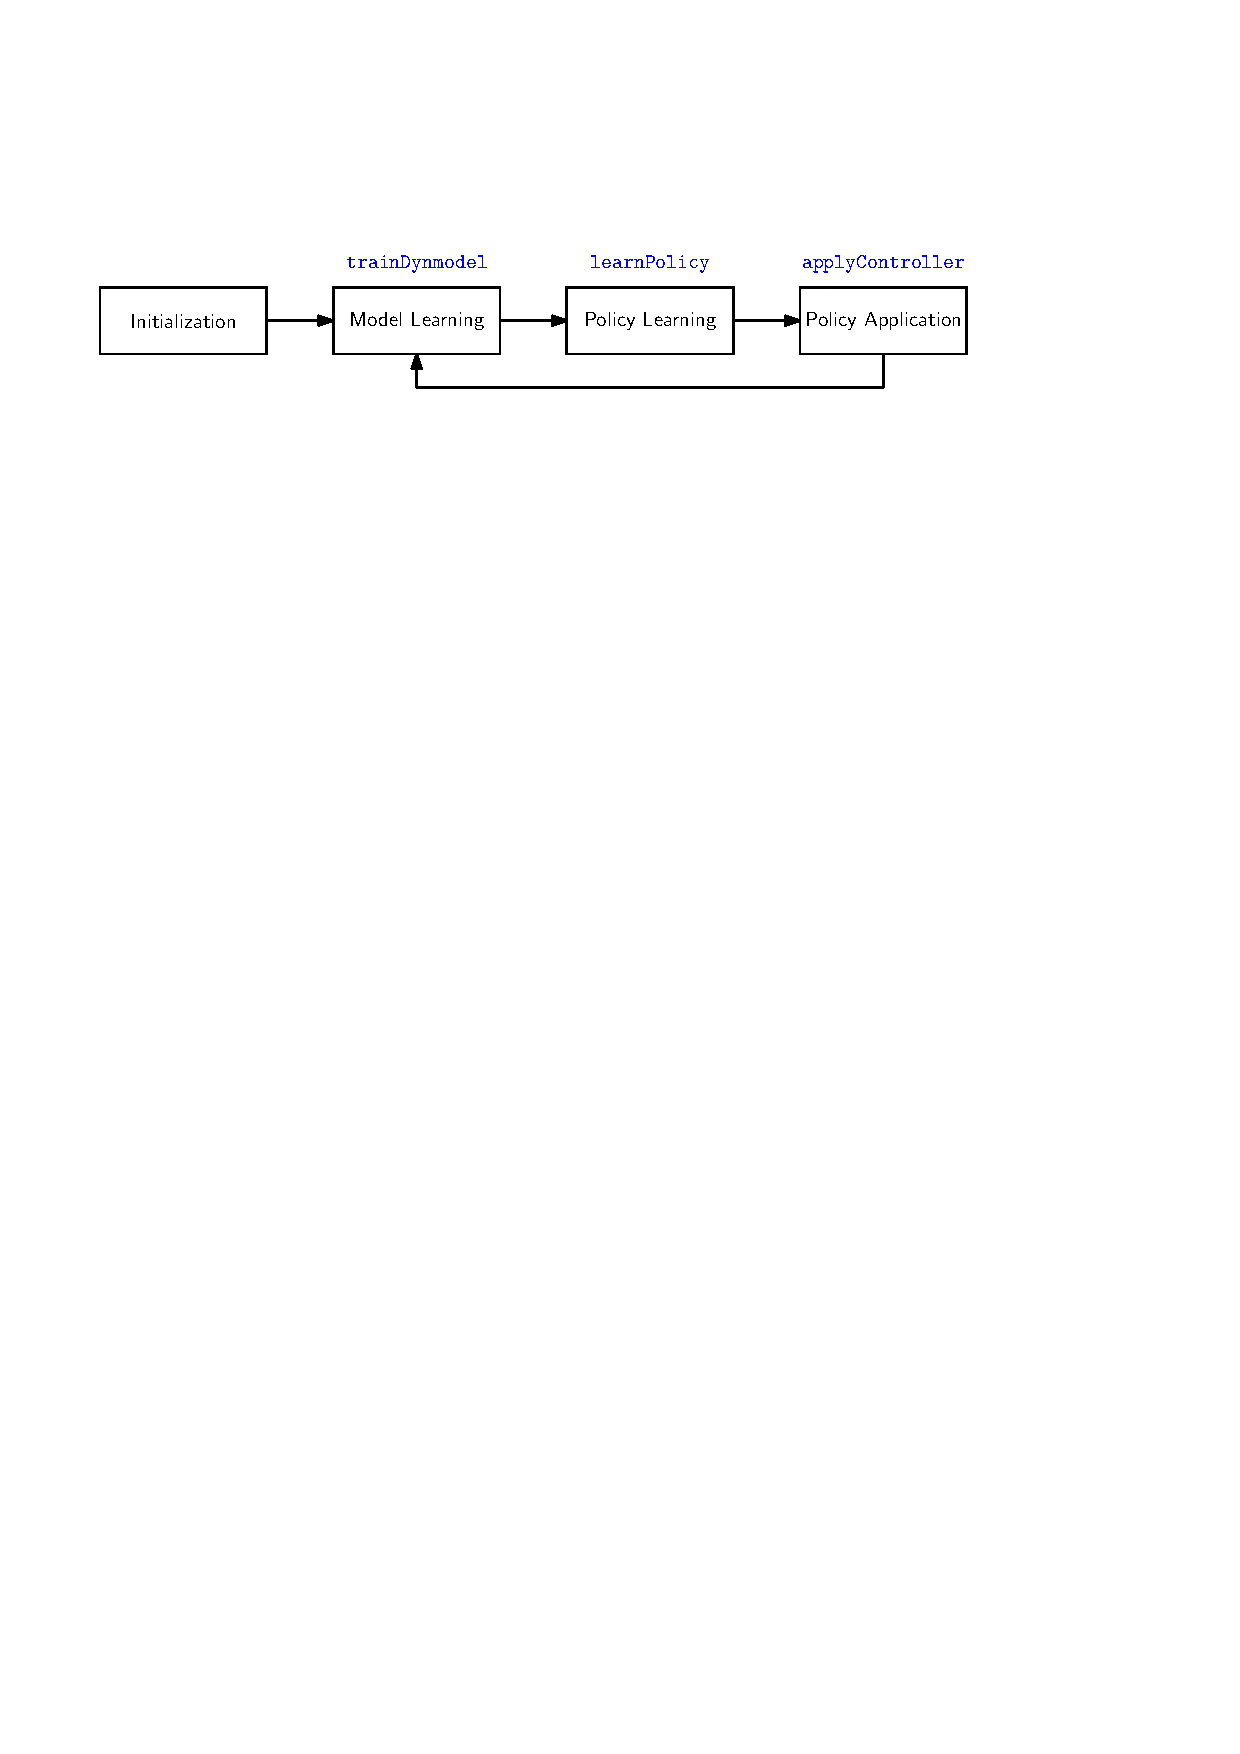
\includegraphics[width = 0.8\hsize]{./figures/flow}
\caption{Main modules: After an initialization, the first module is
  responsible for training a GP from available data. The second module
  is used for policy learning, which consists of policy evaluation and
  improvement. The third module is responsible for applying the
  learned policy to the system, which can be either a simulated system
  or a real system, such as a robot. The collected data from this
  application is used for updating the model, and the cycle starts
  from the beginning.}
\label{fig:modules}
\end{figure}
% general objective



The high-level modules 1) Model learning, 2) Policy learning, 3)
Policy application are summarized in the following.
% function modules
\subsection{Model Learning}

The forward model learned is a non-parametric, probabilistic Gaussian
process~\cite{Rasmussen2006}. The non-parametric property of the GP
does not require an explicit task-dependent parametrization of the
dynamics of the system. The probabilistic property of the GP reduces
the effect of model errors.

% training inputs/targets
Inputs to the GP are state-action pairs $(\vec x_t, \vec u_t)$, where
$t$ is a time index. Training targets are either successor states
$\vec x_{t+1}$ or differences $\Delta_t = \vec x_{t+1} - \vec x_t$.

% sparse GP
By default, a full GP model is trained by evidence maximization, where
we penalize high signal-to-noise ratios in order to maintain numerical
stability. There is an option to switch to sparse GPs in case the
number of data points exceeds a particular threshold. We implemented
the FITC\slash SPGP sparse GP method proposed by \cite{Snelson2006}
for GP training and predictions at uncertain inputs.



\subsection{Policy Learning}
For policy learning, \textsc{pilco} uses the learned GP forward model
to compute approximate long-term predictions $p(\vec x_1|\pi),\dotsc,
p(\vec x_T|\pi)$ for a given controller $\pi$. To do so, we follow the
analytic moment-matching approach proposed
by~\cite{Quinonero-Candela2003a}, and approximate all $p(\vec
x_t|\pi)$ by Gaussians $\gaussx{\vec x_t}{\vec\mu_t}{\mat\Sigma_t}$.

\textbf{Policy Evaluation.}
Once the long-term predictions $p(\vec x_1|\pi),\dotsc, p(\vec
x_T|\pi)$ are computed, the expected long-term cost
%
\begin{align}
  J^\pi = \sum_{t=1}^T \E[c(\vec x_t)\vert\pi]\,,\qquad p(\vec x_0) =
  \gauss{\vec\mu_0}{\mat\Sigma_0}\,,
\end{align}
% 
can be computed analytically for many cost functions $c$, e.g.,
polynomials, trigonometric functions, or Gaussian-shaped functions. In
our implementation, we typically use a Gaussian-shaped cost function
%
\begin{align*}
c(\vec x) = 1-\exp\big(-\tfrac{1}{2}\|\vec x - \vec
x_{\text{target}}\|^2_{\mat W}/\sigma_c^2\big)\,, 
\end{align*}
% 
where $\|\vec x - \vec x_{\text{target}}\|^2_{\mat W}$ is the
Mahalanobis distance between $\vec x$ and $\vec x_{\text{target}}$,
weighted by $\mat W$, $\sigma_c$ is a scaling factor, and $\vec
x_{\text{target}}$ is a target state.

\textbf{Policy Improvement.}  To improve the policy, we use
gradient-based Quasi-Newton optimization methods, such as BFGS. The
required gradients of the expected long-term cost $J^\pi$ with respect
to the policy parameters are computed analytically, which allows for
learning low-level policies with hundreds of
parameters~\cite{Deisenroth2011c}.

\subsection{Policy Application}
This module takes care of applying the learned controller to the
(simulated) system. At each time step $t$, the learned controller
$\pi$ computes the corresponding control signal $\vec u_t$ from the
current state $\vec x_t$. An ODE solver is used to determine the
corresponding successor state $\vec x_{t+1}$. The module returns a
trajectory of state-action pairs, from which the training inputs and
targets for the GP model can be extracted.

If the controller is applied to a real system, such as a robot, this
module is not necessary. Instead, state estimation and control
computation need to be performed on the robot
directly~\cite{Deisenroth2011b}.


\newpage

\section{User Interface by Example}


\begin{lstlisting}
% 0. Initialization
settings;                   % load scenario-specific settings

for jj = 1:J                % Initial J random rollouts
  [xx, yy, realCost{jj}, latent{jj}] = ...
    rollout(gaussian(mu0, S0), struct('maxU',policy.maxU), H, plant, cost);
  x = [x; xx]; y = [y; yy]; % augment training sets for dynamics model  
end

% Controlled learning (N iterations)
for j = 1:N
  % 1. Train (GP) dynamics model
  trainDynModel;  
        
  % 2. Learn policy       
  learnPolicy;                    

  % 3. Apply controller to system
  applyController;                
end
\end{lstlisting}


In line 2, a scenario-specific settings script is executed. Here, we
have to define the policy structure (e.g., parametrization, torque
limits), the cost function, the
dynamics model (e.g., definition of training inputs\slash targets),
 some details about the system\slash plant (e.g., sampling
frequency) that are needed for the ODE solver, and some general
parameters (e.g., prediction horizon, discount factor).

In lines 4--8, we create an initial set of trajectory rollouts by
applying random actions to the system, starting from a state
$\vec x_0$ sampled from $p(\vec x_0)=\gauss{\vec \mu_0, \mat
  S_0}$. The \texttt{rollout} function in line 6 takes care of
this. For each trajectory, the training inputs and targets are
collected in the matrices \texttt{x} and \texttt{y}, respectively.

In lines 11--20, the three main modules are executed
iteratively. First, the GP dynamics model is learned in the
\texttt{trainDynModel} script, using the current training data
\texttt{x,y} (line 13). Second, the policy is learned in the
\texttt{learnPolicy} script, which updates the policy parameters using
analytic policy evaluation and policy gradients. The third module,
i.e., the application of the learned controller to the system, is
encapsulated in the \texttt{applyController} script, which also
augments the current data set \texttt{x,y} for training the GP model
with the new trajectory.

\section{Quick Start}
If you want to try it out without diving into the details, navigate to
\texttt{\path scenarios/cartPole} and execute the
\texttt{cartPole\_learn} script.

\chapter{Software Package Overview}

This software package implements the \textsc{pilco} reinforcement
learning framework~\cite{Deisenroth2011c}. The package contains the
following directories

\begin{itemize}
\item \texttt{base:} Root directory. Contains all other directories.
\item \texttt{control:} Directory that implements several controllers.
\item \texttt{doc:} Documention
\item \texttt{gp:} Everything that has to do with Gaussian processes
  (training, predictions, sparse GPs etc.)
\item \texttt{loss:} Several immediate cost functions
\item \texttt{scenarios:} Different scenarios. Each scenario is
  packaged in a separate directory with all scenario-specific files
\item \texttt{util:} Utility files
\item \texttt{test:} Test functions (derivatives etc.)
\end{itemize}

\section{Main Modules}
The main modules of the \textsc{pilco} framework and their interplay
are visualized in Figure~\ref{fig:modules}. Each module is implemented in
a separate script and can be found in \texttt{\path base}. 
%


Let us have a look at the high-level functionality of the three main
modules in Figure~\ref{fig:modules}:
\begin{enumerate}
\item \texttt{applyController}
\begin{enumerate}
\item determine start state
\item generate rollout
\begin{enumerate}
\item compute control signal $\pi(\vec x_t)$
\item simulate dynamics (or apply control to real robot)
\item transition to state $\vec x_{t+1}$
\end{enumerate}
\end{enumerate}
\item \texttt{trainDynModel}
\item \texttt{learnPolicy}
\begin{enumerate}
\item call gradient-based non-convex optimizer \texttt{minimize}:
  minimize \texttt{value} with respect to policy parameters
  $\vec\theta$
\begin{enumerate}
\item \texttt{propagated:} compute successor state distribution
  $p(\vec x_{t+1})$ and gradients $\partial p(\vec
  x_{t+1})/\partial\vec\theta$ with respect to the policy parameters
  and gradients $\partial p(\vec x_{t+1})/\partial p(\vec x_t)$ with respect
  to the previous state distribution $p(\vec x_t)$.
\begin{enumerate}
\item trigonometric augmentation of the state distribution $p(\vec
  x_t)$
\item compute distribution of preliminary (unsquashed) policy
  $p(\tilde\pi(\vec x_t))$
\item compute distribution of squashed (limited-amplitude) policy
  $p(\pi(\vec x_t))=p(\vec u_t)$
\item determine successor state distribution $p(\vec x_{t+1})$ using
  GP prediction (\texttt{gp*})
\end{enumerate}
\item \texttt{cost.fcn:} Scenario-specific function that computes the
  expected (immediate) cost $\E_{\vec x}[c(\vec x)]$ and its partial derivatives
  $\partial\E_{\vec x}[c(\vec x)]/\partial p(\vec x)$
\end{enumerate}
\end{enumerate}
\end{enumerate}


\subsection{\texttt{applyController}}
\begin{lstlisting}
% 1. Generate trajectory rollout given the current policy
if isfield(plant,'constraint'), HH = maxH; else HH = H; end
[xx, yy, realCost{j+J}, latent{j}] = ...
  rollout(gaussian(mu0, S0), policy, HH, plant, cost);
disp(xx);                           % display states of observed trajectory
x = [x; xx]; y = [y; yy];                            % augment training set
if plotting.verbosity > 0
  if ~ishandle(3); figure(3); else set(0,'CurrentFigure',3); end
  hold on; plot(1:length(realCost{J+j}),realCost{J+j},'r'); drawnow;
end

% 2. Make many rollouts to test the controller quality
if plotting.verbosity > 1
  lat = cell(1,10);
  for i=1:10
    [~,~,~,lat{i}] = rollout(gaussian(mu0, S0), policy, HH, plant, cost);
  end

  if ~ishandle(4); figure(4); else set(0,'CurrentFigure',4); end; clf(4);

  ldyno = length(dyno);
  for i=1:ldyno       % plot the rollouts on top of predicted error bars
    
    subplot(ceil(ldyno/sqrt(ldyno)),ceil(sqrt(ldyno)),i); hold on;
    errorbar( 0:length(M{j}(i,:))-1, M{j}(i,:), ...
      2*sqrt(squeeze(Sigma{j}(i,i,:))) );
    for ii=1:10
      plot( 0:size(lat{ii}(:,dyno(i)),1)-1, lat{ii}(:,dyno(i)), 'r' );
    end
    plot( 0:size(latent{j}(:,dyno(i)),1)-1, latent{j}(:,dyno(i)),'g');
    axis tight
  end
  drawnow;
end

% 3. Save data
filename = [basename num2str(j) '_H' num2str(H)]; save(filename);
\end{lstlisting}

The script \texttt{applyController} executes the following high-level
steps:
\begin{enumerate}
\item Generate a trajectory rollout by applying the current policy to
  the system (lines 1--4). The initial state is sampled from $p(\vec
  x_0)=\mathcal N(\texttt{mu0},\texttt{S0})$, see line 4. This
  trajectory is used to augment the GP training set (line 6).
\item (optional) Generate more trajectories with different start
  states $\vec x_0\sim p(\vec x_0)$ and plot a sample distribution of
  the trajectory distribution (lines 12-- 33).
\item Save the entire workspace (line 36).
\end{enumerate}




\subsection{\texttt{trainDynModel}}
\begin{lstlisting}
% 1. Train GP dynamics model
Du = length(policy.maxU); Da = length(plant.angi); % no. of ctrl and angles
xaug = [x(:,dyno) x(:,end-Du-2*Da+1:end-Du)];     % x augmented with angles
dynmodel.inputs = [xaug(:,dyni) x(:,end-Du+1:end)];     % use dyni and ctrl
dynmodel.targets = y(:,dyno);
dynmodel.targets(:,difi) = dynmodel.targets(:,difi) - x(:,dyno(difi));

dynmodel = dynmodel.train(dynmodel, plant, trainOpt);  %  train dynamics GP

% display some hyperparameters
Xh = dynmodel.hyp;
% noise standard deviations
disp(['Learned noise std: ' num2str(exp(Xh(end,:)))]);
% signal-to-noise ratios (values > 500 can cause numerical problems)
disp(['SNRs             : ' num2str(exp(Xh(end-1,:)-Xh(end,:)))]);
\end{lstlisting}

The script that takes care of training the GP executes the following
high-level steps:
\begin{enumerate}
\item Extract states and controls from \texttt{x}-matrix (lines 2--3)
\item Define the training inputs and targets of the GP (lines 4--6)
\item Train the GP (line 8)
\item Display GP hyper-parameters, the learned noise hyper-parameters,
  and the signal-to-noise ratios (lines 10--15). This information is
  very valuable for debugging purposes.
\end{enumerate}


\subsection{\texttt{learnPolicy}}
\begin{lstlisting}
% 1. Update the policy
opt.fh = 1;
[policy.p fX3] = minimize(policy.p, 'value', opt, mu0Sim, S0Sim, ...
  dynmodel, policy, plant, cost, H);

% (optional) Plot overall optimization progress
if exist('plotting', 'var') && isfield(plotting, 'verbosity') ...
    && plotting.verbosity > 1
  if ~ishandle(2); figure(2); else set(0,'CurrentFigure',2); end
  hold on; plot(fX3); drawnow; 
  xlabel('line search iteration'); ylabel('function value')
end

% 2. Predict trajectory from p(x0) and compute cost trajectory 
[M{j} Sigma{j}] = pred(policy, plant, dynmodel, mu0Sim(:,1), S0Sim, H);
[fantasy.mean{j} fantasy.std{j}] = ...
  calcCost(cost, M{j}, Sigma{j}); % predict cost trajectory

% (optional) Plot predicted immediate costs (as a function of the time steps)
if exist('plotting', 'var') && isfield(plotting, 'verbosity') ...
    && plotting.verbosity > 0
  if ~ishandle(3); figure(3); else set(0,'CurrentFigure',3); end
  clf(3); errorbar(0:H,fantasy.mean{j},2*fantasy.std{j}); drawnow;
  xlabel('time step'); ylabel('immediate cost');
end

\end{lstlisting}

\begin{figure}[ht]
\centering
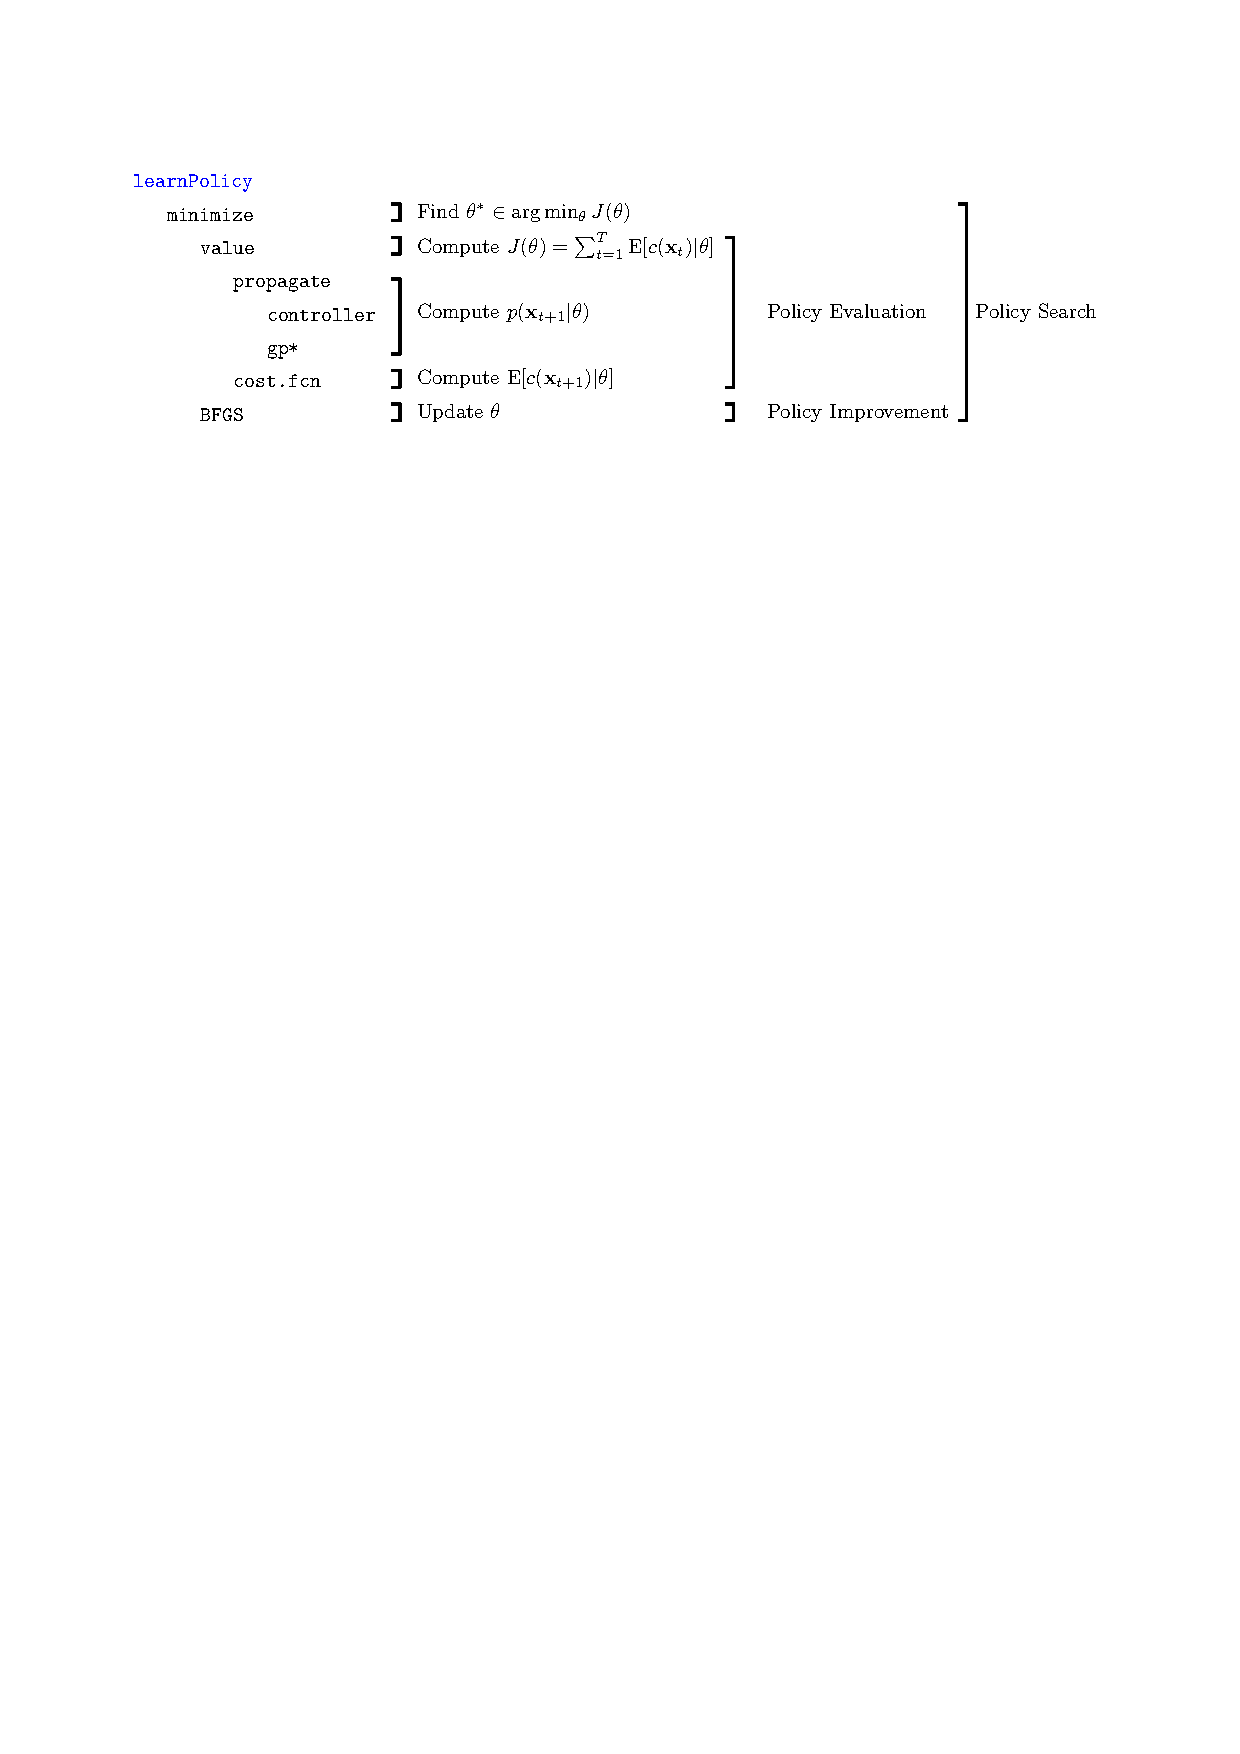
\includegraphics[width = \hsize]{./figures/learnP}
\caption{Functions being called from \texttt{learnPolicy.m} for
  learning the policy.}
\label{fig:learnP}
\end{figure}



\begin{enumerate}
\item Learn the policy by calling
  \texttt{minimize}. Figure~\ref{fig:learnP} depicts the functions
  that are called by \texttt{learnPolicy} in order to perform the
  policy search to find a good parameter set $\vec\theta^*$.
\item (optional) Plot overall optimization progress.
\item Long-term prediction of a state trajectory from $p(\vec x_0)$
  using the learned policy (line 15) by calling \texttt{pred}. This
  prediction is equivalent to the last predicted trajectory during
  policy learning, i.e., the predicted state trajectory that belongs
  to the the learned controller.
\item The predicted state trajectory is used to compute the
  corresponding distribution over immediate costs (lines 16--17) by
  calling \texttt{calcCost}.
\item (optional) Plot the predicted immediate cost distribution as a
  function of the time steps (lines 19--25).
\end{enumerate}

\section{Working with a Real Robot}
When you want to apply \textsc{pilco} to a learning controller
parameters for a real robot, only a few modifications are
necessary. As policy learning is not real-time anyway, it does not
make too much sense performing it on the robot directly. Therefore,
the robot only needs to know about the learned policy, but nothing
about the learned dynamics model.

Here is a list of modifications:
\begin{itemize}
\item An ODE does not need to be specified for simulating the system.
\item All trajectory rollouts are executed directly on the robot.
\item The module \texttt{applyController} needs to take care of
  generating a trajectory on the robot.
\item For generating a trajectory using the robot, the probably least
  coding extensive approach is the following:
\begin{enumerate}
\item Learn the dynamics model and the policy.
\item Save the learned policy parameters in a file.
\item Transfer the parameters to your robot
\item Write a controller function in whatever programming language the
  robot needs.
\item When the controller is applied, just map the measured state
  through the policy to obtain the desired control signal.
\item Save the recorded trajectory in a file and make it available to
  \textsc{pilco} and save them in \texttt{xx, yy}.
\end{enumerate}
\end{itemize}

Here is a high-level code-snippet that explains the main steps.
\begin{lstlisting}
% 0. Initialization
settings;                   % load scenario-specific settings

applyController_on_robot;   % collect data from robot

% Controlled learning (N iterations)
for j = 1:N
  % 1. Train (GP) dynamics model
  trainDynModel;  
        
  % 2. Learn policy       
  learnPolicy;                    

  % 3. Apply controller to system
  applyController_on_robot;                
end
\end{lstlisting}

We successfully applied this procedure on different hardware
platforms~\cite{Deisenroth2011b, Deisenroth2011c}.


\chapter{Important Function Interfaces}
The \textsc{pilco} software package relies on several high-level
functionalities with unified interfaces: 
\begin{itemize}
\item Predicting with GPs when the test input is Gaussian
  distributed. We have implemented several versions of GPs (including
  sparse GPs), which perform these predictions. The generic interface
  is detailed in the following.
\item Controller functions. With a unified interface, it is
  straightforward to swap between controllers in a learning scenario. We
  discuss the generic interface in this chapter.
\item Cost functions. With this software package, we ship
  implementations of several cost functions. The interface of them is
  discussed in this chapter.
\end{itemize}


\section{GP Predictions}
%
Table~\ref{tab:gpP overview} gives an overview of all implemented
functions that are related to predicting with GPs at a Gaussian
distributed test input $\vec x_*\sim \mathcal
N(\vec\mu_*,\mat\Sigma_*)$.
%
\begin{table}[ht]
\centering
\caption{Overview of functions for GP predictions with Gaussian
  distributed test inputs.}
\label{tab:gpP overview}
\begin{tabular}{l|ccc|cc}
& \texttt{[M S V]} & \texttt{[dMdm dSdm  dVdm dMds dSds
  dVds]} & \texttt{[dMdP dSdP dVdP]} & sparse & prob. GP\\
\hline
\texttt{gp0} & \cmark &  \xmark & \xmark & \xmark & \cmark \\
\texttt{gp0d}& \cmark &  \cmark & \xmark & \xmark & \cmark\\
\hline
\texttt{gp1} & \cmark &  \xmark & \xmark & \cmark & \cmark\\
\texttt{gp1d}& \cmark &  \cmark & \xmark & \cmark & \cmark\\
\hline
\texttt{gp2} & \cmark &  \xmark & \xmark & \xmark & \xmark\\
\texttt{gp2d}& \cmark &  \cmark & \cmark & \xmark & \xmark  
\end{tabular}
\end{table}
%
 We assume that the input dimension is $D$
and the predictive dimension is $E$. All functions are in the
directory \texttt{\path gp/}.

The convention in the function name is that a ``\texttt{d}'' indicates
that derivatives are computed. For instance, \texttt{gp0d} computes
the same function values as \texttt{gp0}, but it additionally computes
some derivatives. We have three different categories of functions for
GP predictions:
\begin{itemize}
\item \texttt{gp0}: The underlying model is a full probabilistic GP
  model. This model is used for implementing the standard GP dynamics
  model.
\item \texttt{gp1}: The underlying model is a sparse GP model. In
  particular, we use the SPGP/FITC approach by Snelson and
  Ghahramani~\cite{Snelson2006}. This model is used for implementing
  the GP dynamics when the data set is too large.
\item \texttt{gp2}: The underlying model is a full ``deterministic''
  GP model. The model differs from the full probabilistic model
  (\texttt{gp0}) by ignoring the posterior uncertainty about the
  underlying function. The model essentially consists of the mean
  function only.  This makes it functionally equivalent to a
  radial-basis-function (RBF) network. This kind of model is used for
  implementing nonlinear controllers.
\end{itemize}

\subsection{Input Arguments}

For all functions \texttt{gp*}, the input arguments are the following:
\begin{enumerate}
\item \texttt{gpmodel}: Structure containing all relevant information
\begin{itemize}
\item \texttt{.hyp}: log-hyper-parameters in a $(D+2)\times E$ matrix
  ($D$ log-length scales, 1 log-signal-standard deviation, 1
  log-noise-standard deviation per predictive dimension)
\item \texttt{.inputs}: training inputs in an $n\times D$ matrix
\item \texttt{.targets}: training targets in an $n\times E$ matrix
\end{itemize}
\item \texttt{m}: Mean of the state distribution $p(\vec x)$,  $(D\times 1)$
\item \texttt{s}: Covariance matrix of the state distribution $p(\vec
  x)$, $(D\times D)$
\end{enumerate}

\subsection{Output Arguments}
The \texttt{gp*} functions can be used to compute the mean and the
covariance of the joint distribution $p(\vec x, f(\vec x))$, where
$f\sim \mathcal{GP}$ and $\vec x\sim\mathcal N(\texttt{m},
\texttt{s})$.


All functions \texttt{gp*} predict the mean \texttt{M} and the
covariance \texttt{S} of $p(f(\vec x))$ as well as
\texttt{V}=$\texttt{s}\inv\cov[\vec x, f(\vec x)]$. Note that
\texttt{gp1*} compute these values using sparse GPs and \texttt{gp2*}
use only the mean function of the GP, i.e., the posterior uncertainty
about $f$ is discarded.

For policy learning, we require from the \emph{dynamics model} the
following derivatives:
\begin{itemize}
\item \texttt{dMdm:} $\partial M/\partial m\in\R^{E\times D}$ The
  derivative of the mean of the prediction with respect to the
  mean of the input distribution.
\item \texttt{dSdm:} $\partial S/\partial m\in\R^{E^2\times D}$ The
  derivative of the covariance of the prediction with respect to the
  mean of the input distribution.
\item \texttt{dVdm:} $\partial V/\partial m\in\R^{DE\times D}$ The
  derivative of $V$ with respect to the
  mean of the input distribution.
\item \texttt{dMds:} $\partial M/\partial s\in\R^{E\times D^2}$ The
  derivative of the mean of the prediction with respect to the
  covariance of the input distribution.
\item \texttt{dSds:} $\partial S/\partial m\in\R^{E^2\times D^2}$ The
  derivative of the covariance of the prediction with respect to the
  covariance of the input distribution.
\item \texttt{dVds:} $\partial V/\partial m\in\R^{DE\times D^2}$ The
  derivative of  $V$ with respect to the
  covariance of the input distribution.
\end{itemize}
As \texttt{gp0d} and \texttt{gp1d} are the functions used to propagate
uncertainties through a GP dynamics model, they all compute these
derivatives, see Table~\ref{tab:gpP overview}.



% additional derivatives for policy 
When we use \texttt{gp2*} as a convenient implementation of an RBF
network \emph{controller}, we additionally require the gradients of
\texttt{M, S, V} with respect to the ``parameters'' of the GP, which
are abbreviated by \texttt{P} in Table~\ref{tab:gpP overview}. These
parameters comprise the training inputs, the training targets, and the
log-hyper-parameters:
\begin{itemize}
\item \texttt{dMdP}$=\{\partial M/\partial X, \partial M/\partial
  y, \partial M/\partial\theta \}$: The derivative of the mean
  prediction with respect to the training inputs $X$, the training
  targets $y$, and the log-hyper-parameters $\theta$.
\item \texttt{dSdP}$=\{\partial S/\partial X, \partial S/\partial
  y, \partial S/\partial\theta \}$: The derivative of the covariance
  of the prediction with respect to the training inputs $X$, the
  training targets $y$, and the log-hyper-parameters $\theta$.
\item \texttt{dVdP}$=\{\partial V/\partial X, \partial V/\partial
  y, \partial V/\partial\theta \}$: The derivative of \texttt{V} with
  respect to the training inputs $X$, the training targets $y$, and
  the log-hyper-parameters $\theta$.
\end{itemize}


\section{Controller}
The control directory is located at \path\texttt{control}. The
controllers compute the (unconstrained) control signals
$\tilde\pi(\vec x)$.

The generic function call is as follows, where 
\texttt{controller} is a generic name\footnote{We have implemented two
  controller functions: \texttt{conlin} and \texttt{congp}}:
\begin{lstlisting}
function [M, S, V, dMdm, dSdm, dCdm, dMds, dSds, dVds, dMdp, dSdp, dVdp] ...
         = controller(policy, m, s)
\end{lstlisting}


\subsection{Interface}
Let us explain the interface in more detail
\subsubsection{Input Arguments}
All controllers expect the following inputs
\begin{enumerate}
\item \texttt{policy:} A struct with the following fields
\begin{itemize}
\item \texttt{policy.fcn}: A function handle to \texttt{controller}. This is
  not needed by the controller function itself, but by other functions
  that call \texttt{controller}.
\item \texttt{policy.p}: The policy parameters. Everything that is in this
  field is considered a free parameter and optimized during policy
  learning.
\item \texttt{policy.<>}: Other arguments the controller function requires.
\end{itemize}
\item \texttt{m}: $\E[\vec x]\in\R^D$ The mean of the state
  distribution $p(\vec x)$.
\item \texttt{s}: $\var[\vec x]\in\R^{D\times D}$ The covariance
  matrix of the state distribution $p(\vec x)$.
\end{enumerate}


\subsubsection{Output Arguments}
All controller functions are expected to compute
\begin{enumerate}
\item \texttt{M:} $\E[\tilde\pi(\vec x)]\in\R^F$ The mean of the
  predicted (unconstrained) control signal
\item \texttt{S:} $\var[\tilde\pi(\vec x)]\in\R^{F\times F}$ The
  covariance matrix of the predicted (unconstrained) control signal
\item \texttt{V:} $\var(\vec x)\inv\cov[\vec x,\tilde\pi(\vec x)]$ The
  cross-covariance between the (input) state $\vec x$ and the control
  signal $\tilde\pi(\vec x)$, pre-multiplied with $\var(\vec x)\inv$,
  the inverse of the covariance matrix of $p(\vec x)$. We do not
  compute $\cov[\vec x,\tilde\pi(\vec x)]$ because of numerical
  reasons.
\item Gradients. The gradients of all output arguments with
  respect to all input arguments are computed:
\begin{itemize}
\item \texttt{dMdm:} $\partial M/\partial m\in\R^{F\times D}$ The
  derivative of the mean of the predicted control with respect to the
  mean of the state distribution.
\item \texttt{dSdm:} $\partial S/\partial m\in\R^{F^2\times D}$ The
  derivative of the covariance of the predicted control with respect to the
  mean of the state distribution.
\item \texttt{dVdm:} $\partial V/\partial m\in\R^{DF\times D}$ The
  derivative of $V$ with respect to the
  mean of the state distribution.
\item \texttt{dMds:} $\partial M/\partial s\in\R^{F\times D^2}$ The
  derivative of the mean of the predicted control with respect to the
  covariance of the state distribution.
\item \texttt{dSds:} $\partial S/\partial m\in\R^{F^2\times D^2}$ The
  derivative of the covariance of the predicted control with respect to the
  covariance of the state distribution.
\item \texttt{dVds:} $\partial V/\partial m\in\R^{DF\times D^2}$ The
  derivative of  $V$ with respect to the
  covariance of the state distribution.
\item \texttt{dMdp:} $\partial M/\partial\polpar\in\R^{F\times |\vec\polpar|}$ The
  derivative of the mean of the predicted control with respect to the
  policy parameters $\vec\polpar$.
\item \texttt{dSdp:} $\partial S/\partial\polpar\in\R^{F^2\times |\vec\polpar|}$ The
  derivative of the covariance of the predicted control with respect to the
  policy parameters $\vec\polpar$.
\item \texttt{dVdp:} $\partial V/\partial\polpar\in\R^{DF\times
    |\vec\polpar|}$ The derivative of $V$ with respect to the policy
  parameters $\vec\polpar$.
\end{itemize}
\end{enumerate}

% \begin{verbatim}
% M             mean of the predicted control                      [ F  x  1 ]
% S             covariance of predicted control                    [ F  x  F ]
% C             inv(s)*covariance between input and control        [ D  x  F ]
% dMdm          deriv. of mean control wrt mean of state           [ F  x  D ]
% dSdm          deriv. of control variance wrt mean of state       [F*F x  D ]
% dCdm          deriv. of C wrt mean of state                      [D*F x  D ]
% dMds          deriv. of mean control wrt variance                [ F  x D*D]
% dSds          deriv. of control variance wrt variance            [F*F x D*D]
% dCds          deriv. of C wrt variance                           [D*F x D*D]
% dMdp          deriv. of mean control wrt GP hyper-parameters     [ F  x  P ]
% dSdp          deriv. of control variance wrt GP hyper-parameters [F*F x  P ]
% dCdp          deriv. of C wrt GP hyper-parameters                [D*F x  P ]
% \end{verbatim}


\section{Cost Functions}
Any (generic) cost function is supposed to compute the expected
(immediate) cost $\E[c(\vec x)]$ and the corresponding variance
$\var[c(\vec x)]$ for a Gaussian distributed state $\vec x\sim
\mathcal N(\vec m, \mat S)$. 

Cost functions have to be written for each scenario. Example cost
functions can be found in \texttt{\path scenarios/*}.

\subsection{Interface for Scenario-specific Cost Functions}
\begin{lstlisting}
function [L, dLdm, dLds, S] = loss(cost, m, s)
\end{lstlisting}


\paragraph{Input Arguments}
\begin{verbatim}
cost            cost structure
  .p            parameters that are required to compute the cost,
                e.g., length of pendulum                            [P x  1 ]
  .expl         (optional) exploration parameter
  .target       target state                                        [D x  1 ]
m               mean of state distribution                          [D x  1 ]
s               covariance matrix for the state distribution        [D x  D ]
\end{verbatim}
We only listed typical fields of the \texttt{cost} structure. It is
possible to add more information. \texttt{cost.expl} allows for
UCB-type exploration, in which case the returned cost \texttt{L}
should be computed according to
%
\begin{align}
  L(\vec x) = \E_{\vec x}[c(\vec x)] + \kappa\sqrt{\var_{\vec
      x}[c(\vec x)]}\,,
\label{eq:UCB cost}
\end{align}
% 
where $\kappa$ is an exploration parameter stored in
\texttt{cost.expl}. Exploration is encouraged for $\kappa<0$ and
discouraged for $\kappa > 0$. By default, exploration is disabled,
i.e., \texttt{cost.expl=0}. A target state can be passed in via
\texttt{cost.target}, but could also be hard-coded in the cost
function.


\paragraph{Output Arguments}
\begin{verbatim}
L     expected cost                                                 [1 x  1 ]
dLdm  derivative of expected cost wrt. state mean vector            [1 x  D ]
dLds  derivative of expected cost wrt. state covariance matrix      [1 x D^2]
S     variance of cost                                              [1 x  1 ]   
\end{verbatim}

Note that the expected cost $L=\E[c(\vec x)]$ can take care of
UCB-type exploration, see Equation~\eqref{eq:UCB cost}. The gradients
of \texttt{L} with respect to the mean (\texttt{dLdm}) and covariance
(\texttt{dLds}) of the input distribution are required for policy
learning.

\subsection{General Building Blocks}
We have implemented some generic building blocks that can be called by
the scenario-specific cost functions. In the following, we detail the
computation of a saturating cost function \texttt{\path
  loss/lossSat.m} and a quadratic cost function \texttt{\path
  loss/lossQuad.m}.

\subsubsection{Saturating Cost}


%%%%%% show image...

\texttt{lossSat} computes the expectation and variance of a
saturating cost 
\begin{align*}
  1 - \exp\big(-\tfrac{1}{2}(\vec x - \vec z)\T\mat W(\vec x - \vec
  z)\big)\in[0,1]
\end{align*}
and their derivatives, where $\vec x \sim\mathcal N(\vec m, \mat S)$,
and a is a normalizing constant. The matrix $\mat W$ is never inverted
and plays the role of a precision matrix. Moreover, it is
straightforward to eliminate the influence of state variables in the
cost function by setting the corresponding values in $\mat W$ to 0.


\begin{lstlisting}[name=lossSat]
function [L, dLdm, dLds, S, dSdm, dSds, C, dCdm, dCds] = lossSat(cost, m, s)
\end{lstlisting}

\begin{par}
\textbf{Input arguments:}
\end{par} 

\begin{verbatim}  
cost
  .z:     target state                                               [D x 1]
  .W:     weight matrix                                              [D x D]
m         mean of input distribution                                 [D x 1]
s         covariance matrix of input distribution                    [D x D]
\end{verbatim}

\begin{par}
\textbf{Output arguments:}
\end{par} 

\begin{verbatim}
L               expected loss                                  [1   x    1 ]
dLdm            derivative of L wrt input mean                 [1   x    D ]
dLds            derivative of L wrt input covariance           [1   x   D^2]
S               variance of loss                               [1   x    1 ]
dSdm            derivative of S wrt input mean                 [1   x    D ]
dSds            derivative of S wrt input covariance           [1   x   D^2]
C               inv(S) times input-output covariance           [D   x    1 ]
dCdm            derivative of C wrt input mean                 [D   x    D ]
dCds            derivative of C wrt input covariance           [D   x   D^2]
\end{verbatim}




\subsubsection*{Implementation}
\vspace{-5mm}
\begin{lstlisting}[name=lossSat]
% some precomputations
D = length(m); % get state dimension

% set some defaults if necessary
if isfield(cost,'W'); W = cost.W; else W = eye(D); end
if isfield(cost,'z'); z = cost.z; else z = zeros(D,1); end

SW = s*W;
iSpW = W/(eye(D)+SW);
\end{lstlisting}
In lines 6--7, we check whether the weight matrix $\mat W$ and the
state $\vec z$ exist. Their default values are $\mat I$ and $\vec 0$,
respectively. Lines 9--10 do
some pre-computations of matrices that will be frequently used
afterwards.


\begin{lstlisting}[name=lossSat]
% 1. Expected cost
L = -exp(-(m-z)'*iSpW*(m-z)/2)/sqrt(det(eye(D)+SW)); % in interval [-1,0]

% 1a. derivatives of expected cost
if nargout > 1
  dLdm = -L*(m-z)'*iSpW;  % wrt input mean
  dLds = L*(iSpW*(m-z)*(m-z)'-eye(D))*iSpW/2;  % wrt input covariance matrix
end
\end{lstlisting}
In lines 11--18, we compute the expected cost $L = \E[c(\vec x)]$ and
its derivatives with respect to the mean and the covariance matrix of
the input distribution.  A detailed derivation can be found
in~\cite{Deisenroth2010b}. Note that at the moment,
\texttt{L}$\in[-1,0]$ (line 12).


\begin{lstlisting}[name=lossSat]
% 2. Variance of cost
if nargout > 3
  i2SpW = W/(eye(D)+2*SW);
  r2 = exp(-(m-z)'*i2SpW*(m-z))/sqrt(det(eye(D)+2*SW));
  S = r2 - L^2;
  if S < 1e-12; S=0; end % for numerical reasons
end

% 2a. derivatives of variance of cost
if nargout > 4
  % wrt input mean
  dSdm = -2*r2*(m-z)'*i2SpW-2*L*dLdm;
  % wrt input covariance matrix
  dSds = r2*(2*i2SpW*(m-z)*(m-z)'-eye(D))*i2SpW-2*L*dLds;
end
\end{lstlisting}
In lines 19--33, we compute the variance $\var[c(\vec x)]$ of the cost
and its derivatives with respect to the mean and the covariance matrix
of the input distribution. A detailed derivation can be found
in~\cite{Deisenroth2010b}. If the variance $\var[c(\vec x)]<10^{-12}$,
we set it to 0 for numerical reasons (line 24).


\begin{lstlisting}[name=lossSat]
% 3. inv(s)*cov(x,L)
if nargout > 6
    t = W*z - iSpW*(SW*z+m);
    C = L*t;
    dCdm = t*dLdm - L*iSpW;
    dCds = -L*(bsxfun(@times,iSpW,permute(t,[3,2,1])) + ...
                                    bsxfun(@times,permute(iSpW,[1,3,2]),t'))/2;
    dCds = bsxfun(@times,t,dLds(:)') + reshape(dCds,D,D^2);
end
\end{lstlisting}
If required, lines 34--42 compute $\mat S\inv\cov[\vec x, c(\vec x)]$
and the corresponding derivatives with respect to the mean and the
covariance of the (Gaussian) state distribution $p(\vec x)$.

\begin{lstlisting}[name=lossSat]
L = 1+L; % bring cost to the interval [0,1]
\end{lstlisting}
Line 43 brings the expected cost \texttt{L} to the interval $[0,1]$.


\subsubsection{Quadratic Cost}


\texttt{lossQuad} computes the expectation and variance of a quadratic
cost
\begin{align*}
c(\vec x) = (\vec x - \vec z)\T\mat W(\vec x - \vec z)
\end{align*}
and their derivatives with respect to the mean and covariance matrix
of the (Gaussian) input distribution $p(\vec x)$.

\begin{lstlisting}[name=lossQuad]
function [L, dLdm, dLds, S, dSdm, dSds, C, dCdm, dCds] = lossQuad(cost, m, S)
\end{lstlisting}

\paragraph{Input arguments}


\begin{verbatim}  
cost
  .z:     target state                                               [D x 1]
  .W:     weight matrix                                              [D x D]
m         mean of input distribution                                 [D x 1]
s         covariance matrix of input distribution                    [D x D]
\end{verbatim}
\begin{par}
\textbf{Output arguments}
\end{par}
\begin{verbatim}
L         expected loss                                        [1   x    1 ]
dLdm      derivative of L wrt input mean                       [1   x    D ]
dLds      derivative of L wrt input covariance                 [1   x   D^2]
S         variance of loss                                     [1   x    1 ]
dSdm      derivative of S wrt input mean                       [1   x    D ]
dSds      derivative of S wrt input covariance                 [1   x   D^2]
C         inv(S) times input-output covariance                 [D   x    1 ]
dCdm      derivative of C wrt input mean                       [D   x    D ]
dCds      derivative of C wrt input covariance                 [D   x   D^2]
\end{verbatim}


\subsubsection*{Implementation} 
\vspace{-5mm}

\begin{lstlisting}[name=lossQuad]
D = length(m); % get state dimension

% set some defaults if necessary
if isfield(cost,'W'); W = cost.W; else W = eye(D); end
if isfield(cost,'z'); z = cost.z; else z = zeros(D,1); end
\end{lstlisting}
In lines 5--6, we check whether the weight matrix $\mat W$ and the
state $\vec z$ exist. Their default values are $\mat I$ and $\vec 0$,
respectively.

\begin{lstlisting}[name=lossQuad]
% 1. expected cost
L = S(:)'*W(:) + (z-m)'*W*(z-m);

% 1a. derivatives of expected cost
if nargout > 1
  dLdm = 2*(m-z)'*W; % wrt input mean
  dLds = W';         % wrt input covariance matrix
end
\end{lstlisting}
In lines 7--14, we compute the expected cost $L = \E[c(\vec x)]$ and
its derivatives with respect to the mean and the covariance matrix of
the input distribution.  A detailed derivation can be found
in~\cite{Deisenroth2010b}. 


\begin{lstlisting}[name=lossQuad]
% 2. variance of cost
if nargout > 3
  S = trace(W*S*(W + W')*S) + (z-m)'*(W + W')*S*(W + W')*(z-m);
  if S < 1e-12; S = 0; end % for numerical reasons
end

% 2a. derivatives of variance of cost
if nargout > 4
  % wrt input mean
  dSdm = -(2*(W+W')*S*(W+W)*(z-m))';
  % wrt input covariance matrix
  dSds = W'*S'*(W + W')'+(W + W')'*S'*W' + (W + W')*(z-m)*((W + W')*(z-m))';
end
\end{lstlisting}
In lines 15--27, we compute the variance $\var[c(\vec x)]$ of the cost
and its derivatives with respect to the mean and the covariance matrix
of the input distribution. A detailed derivation can be found
in~\cite{Deisenroth2010b}. If the variance $\var[c(\vec x)]<10^{-12}$,
we set it to 0 for numerical reasons (line 18).

\begin{lstlisting}[name=lossQuad]
% 3. inv(s) times IO covariance with derivatives
if nargout > 6
    C = 2*W*(m-z);
    dCdm = 2*W;
    dCds = zeros(D,D^2);
end
\end{lstlisting}
If required, lines 28--33 compute $\mat S\inv\cov[\vec x, c(\vec x)]$
and the corresponding derivatives with respect to the mean and the
covariance of the (Gaussian) state distribution $p(\vec x)$.


\chapter{How to Create Your Own Scenario}
In this chapter, we explain in sufficient detail how to set up a new
scenario by going step-by-step through the cart-pole scenario, which
can be found in \texttt{\path scenarios/cartPole}.


\section{Necessary Files}
For each scenario, we need the following set of files, which are
specific to this scenario. In the cart-pole case, these files are the
following:
\begin{itemize}
\item \texttt{settings\_cp.m}: A file that contains scenario-specific
  settings and initializations
\item \texttt{loss\_cp.m}: A cost function
\item \texttt{dynamics\_cp.m}: A file that implements the ODE, which governs
  the dynamics.\footnote{When working with a real robot, this file is
    not needed.}
\item \texttt{learn\_cp.m}: A file that puts everything together
\item (optional) visualization
\end{itemize}


\section{ODE Dynamics}

In the following, we briefly describe the interface and the
functionality of the cart-pole dynamics. The \textsc{pilco} code
assumes by default that the dynamics model is given by an ODE that is
solved numerically using ODE45 (see \texttt{\path util/simulate.m} for more
details).

\begin{lstlisting}[name=dynamics_cp] 
function dz = dynamics_cp(t, z, f)
\end{lstlisting}
\textbf{Input arguments:}

\begin{verbatim}
   t     current time step (called from ODE solver)
   z     state                                                    [4 x 1]
   f     (optional): force f(t)
\end{verbatim}
The input arguments are as follows:
\begin{itemize}
\item \texttt{t}: The current time.
\item \texttt{z}: The state. It is assumed that the state $\vec z$ is
  given as follows:
%
\begin{align*}
\vec z = [x, \dot x, \dot\theta, \theta]\,,
\end{align*}
where $x$ is the position of the cart (given in $\unit{m}$), $\dot x$ is
the cart's velocity (in $\unit{m/s}$), $\dot\theta$ is the pendulum's
angular velocity in $\unit{rad/s}$, and $\theta$ is the pendulum's
angle in $\unit{rad}$. For the angle $\theta$, we chose
$\unit[0]{rad}$ to be the angle when the pendulum hangs downward.
\item \texttt{f}: The applied force to the cart.
\end{itemize}
 \begin{par}
\textbf{Output arguments:}
\end{par} \vspace{1em}
\begin{verbatim}
   dz    if 3 input arguments:      state derivative wrt time
         if only 2 input arguments: total mechanical energy
\end{verbatim}
The function returns either $\dot{\vec z}$, if three input arguments
are given, or the total mechanical energy with two input
arguments. The total mechanical energy can be used to verify that the
system preserves energy (here, the friction coefficient in line 5
needs to be set to 0).

\begin{lstlisting}[name=dynamics_cp]
l = 0.5;  % [m]      length of pendulum
m = 0.5;  % [kg]     mass of pendulum
M = 0.5;  % [kg]     mass of cart
b = 0.1;  % [N/m/s]  coefficient of friction between cart and ground
g = 9.82; % [m/s^2]  acceleration of gravity
\end{lstlisting}
In lines 2--6, the parameters of the cart-pole system are defined: the
length of the pendulum \texttt{l} (line 2), the mass of the pendulum
\texttt{m} (line 3), the mass of the cart \texttt{M} (line 4), the
coefficient of friction between cart and ground \texttt{b} (line 5),
and the acceleration of gravity \texttt{g} (line 6).

\begin{lstlisting}[name=dynamics_cp]
if nargin==3
  dz = zeros(4,1);
  dz(1) = z(2);
  dz(2) = ( 2*m*l*z(3)^2*sin(z(4)) + 3*m*g*sin(z(4))*cos(z(4)) ...
          + 4*f(t) - 4*b*z(2) )/( 4*(M+m)-3*m*cos(z(4))^2 );
  dz(3) = (-3*m*l*z(3)^2*sin(z(4))*cos(z(4)) - 6*(M+m)*g*sin(z(4)) ...
          - 6*(f(t)-b*z(2))*cos(z(4)) )/( 4*l*(m+M)-3*m*l*cos(z(4))^2 );
  dz(4) = z(3);
else
  dz = (M+m)*z(2)^2/2 + 1/6*m*l^2*z(3)^2 + m*l*(z(2)*z(3)-g)*cos(z(4))/2;
end
\end{lstlisting}
Lines 7--17 compute either $\dot{\vec z}$ (lines 8--14) or the total
mechanical energy (line 16). A principled derivation of the system
dynamics and the mechanical energy can be found
in~\cite{Deisenroth2010b}.



\section{Scenario-specific Settings}


\subsection{Adding Paths}
%
\begin{lstlisting}[name=settings_cp]
rand('seed',1); randn('seed',1); format short; format compact;
% include some paths
try
  rd = '../../';
  addpath([rd 'base'],[rd 'util'],[rd 'gp'],[rd 'control'],[rd 'loss']);
catch
end
\end{lstlisting}
First, we include (relative) paths to the directories required for
learning and initialize the random seed to make the experiments
reproducible. The setting of the random seeds (line 1) will cause some
warnings in newer versions of MATLAB, but it is backwards compatible
to MATLAB~2007.

\subsection{Indices}
\begin{lstlisting}[name=settings_cp]
% 1. Define state and important indices

% 1a. Full state representation (including all augmentations)
%
%  1  x          cart position
%  2  v          cart velocity
%  3  dtheta     angular velocity
%  4  theta      angle of the pendulum
%  5  sin(theta) complex representation ...
%  6  cos(theta) of theta
%  7  u          force applied to cart
%

% 1b. Important indices
% odei  indicies for the ode solver
% augi  indicies for variables augmented to the ode variables
% dyno  indicies for the output from the dynamics model and indicies to loss
% angi  indicies for variables treated as angles (using sin/cos representation)
% dyni  indicies for inputs to the dynamics model
% poli  indicies for the inputs to the policy
% difi  indicies for training targets that are differences (rather than values)

odei = [1 2 3 4];            % varibles for the ode solver
augi = [];                   % variables to be augmented
dyno = [1 2 3 4];            % variables to be predicted (and known to loss)
angi = [4];                  % angle variables
dyni = [1 2 3 5 6];          % variables that serve as inputs to the dynamics GP
poli = [1 2 3 5 6];          % variables that serve as inputs to the policy
difi = [1 2 3 4];            % variables that are learned via differences
\end{lstlisting}
We now define important state indices that are required by the code
that does the actual learning. We assume that the state is given as
\begin{align*}
\vec x = [x, \dot x, \dot\theta, \theta]\T\,,
\end{align*}
where $x$ is the position of the cart, $\dot x$ the corresponding
velocity, and $\dot\theta$ and $\theta$ are the angular velocity and
the angle of the pendulum.

The ODE-solver requires to know what parts of the state are used for
the forward dynamics. These indices are captured by $\texttt{odei}$
(line 30).

The predictive dimensions of the dynamics GP model are stored in
\texttt{dyno} (line 32). 

The indices in $\texttt{angi}$ (line 33) indicate which variables are
angles. We represent these angle variables in the complex plane
%
\begin{align*}
  \theta \mapsto [\sin\theta, \cos\theta]\T
\end{align*}
% 
to be able to exploit the wrap-around condition $\theta\equiv
\theta+2k\pi$, $k\in\mathds{Z}$. With this augmentation, we define the
auxiliary state vector, i.e., the state vector augmented with the
complex representation of the angle, as
%
\begin{align}
  \vec x = [x, \dot x, \dot\theta, \theta, \sin\theta,
  \cos\theta]\T\,.
\label{eq:aux state}
\end{align}
% 

The \texttt{dyni} indices (line 34) describe which variables from the
auxiliary state vector in Equation~\eqref{eq:aux state} are used as
the training inputs for the GP dynamics model. Note that we use the
complex representation $[\sin\theta, \cos\theta]$ instead of $\theta$,
i.e., we no longer need $\theta$ in the inputs of the dynamics GP.

The \texttt{poli} indices (line 35) describe which state variables
from the auxiliary state vector in Equation~\eqref{eq:aux state} are
used as inputs to the policy.

The \texttt{difi} indices (line 36) are a subset of $\texttt{dyno}$
and contain the indices of the state variables for which the GP
training targets are differences
%
\begin{align*}
\Delta_t = \vec x_{t+1} - \vec x_t
\end{align*}
% 
instead of $\vec x_{t+1}$. Using differences as training targets
encodes an implicit prior mean function $m(\vec x) = \vec x$. This
means that when leaving the training data, the GP predictions do not
fall back to 0 but they remain constant. A practical implication is
that learning differences $\Delta_t$ generalizes better across
different parts of the state space.  From a learning point of view,
training a GP on differences is much simpler than training it on
absolute values: The function to be learned does not vary so much,
i.e., we do not need so many data points in the end. From a robotics
point of view, robot dynamics are typically relative to the current
state, they do not so much depend on absolute coordinates.


\subsection{General Settings}

\begin{lstlisting}[name=settings_cp]
% 2. Set up the scenario
dt = 0.10;                         % [s] sampling time
T = 4.0;                           % [s] initial prediction horizon time
H = ceil(T/dt);                    % prediction steps (optimization horizon)
mu0 = [0 0 0 0]';                  % initial state mean
S0 = diag([0.1 0.1 0.1 0.1].^2);   % initial state covariance
N = 15;                            % number controller optimizations
J = 1;                             % initial J trajectories of length H
K = 1;                             % no. of initial states for which we optimize
nc = 100;                          % number of controller basis functions
\end{lstlisting}


\texttt{dt} is the sampling time, i.e., $1/dt$ is the sampling
frequency. 

\texttt{T} is the length of the prediction horizon in seconds.

\texttt{H}$=T/dt$ is the length of the prediction horizon in time
steps.

\texttt{mu0} is the mean of the distribution $p(\vec x_0)$ of the
initial state. Here, \texttt{mu0}$=\vec 0$ encodes that the cart is
in the middle of the track (with zero velocity) with the pendulum
hanging down (with zero angular velocity).

\texttt{S0} is the covariance matrix of $p(\vec x_0)$.

\texttt{N} is the number of times the loop in Figure~\ref{fig:modules}
is executed.

\texttt{J} is the number of initial random rollouts, i.e., rollouts
with a random policy. These rollouts are used to collect an initial
data set for training the first GP dynamics model. Usually, we set
this to 1.

\texttt{K} is the number of initial states for which the policy is
learned. The code can manage initial state distributions of the form
%
\begin{align}
p(\vec x_0) \propto \sum_{i=1}^K \mathcal N(\vec\mu_{0}^{(i)}, \mat\Sigma_0)\,,
\end{align}
% 
which corresponds to a distributions with different means
$\vec\mu_0^{(i)}$ but shared covariance matrices $\Sigma_0$.

\texttt{nc} is the number of basis functions of the policy. In this
scenario, we use a nonlinear policy of the form
%
\begin{align}
  \pi(\vec x) &= u_{\max}\sigma\tilde\pi(\vec x)\label{eq:squashed rbf policy}\\
  \tilde\pi(\vec x) &= \sum_{i=1}^{\texttt{nc}} w_i 
  \exp\big(-\tfrac{1}{2}(\vec x - \vec c_i)\T\mat W(\vec x - \vec
  c_i)\big)\label{eq:unsquashed rbf policy}\,,
\end{align}
% 
where $\sigma$ is a squashing function, which maps its argument to the
interval $[-1,1]$, $\vec c_i$ are the locations of the Gaussian-shaped
basis functions, and $\mat W$ is a (shared) weight matrix. 

\begin{figure}[tb]
\centering
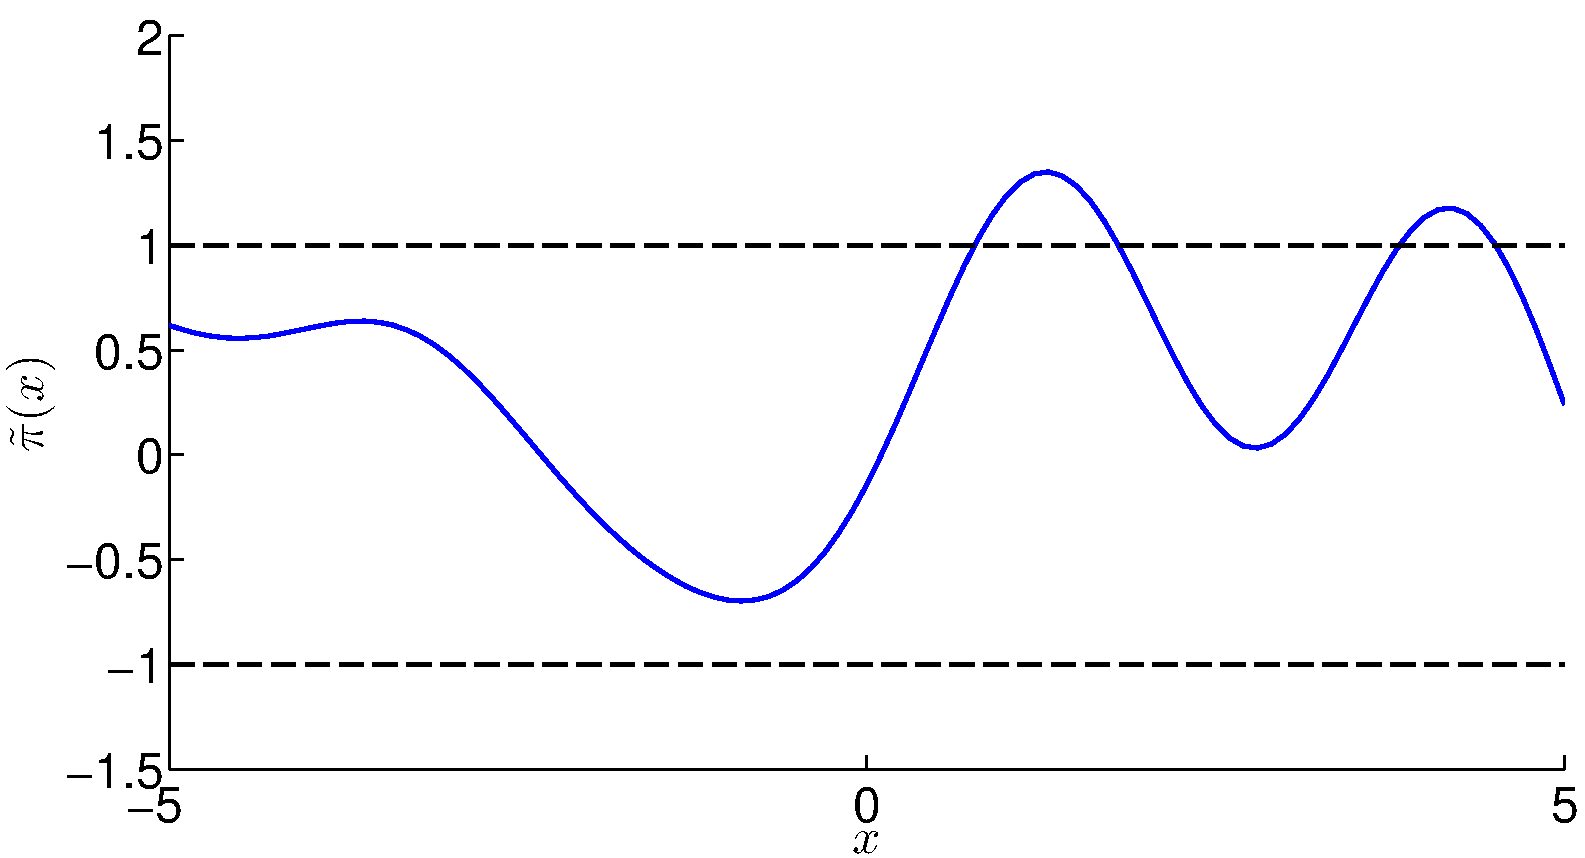
\includegraphics[width = 0.45\hsize]{./figures/preliminary_policy}
\hspace{5mm}
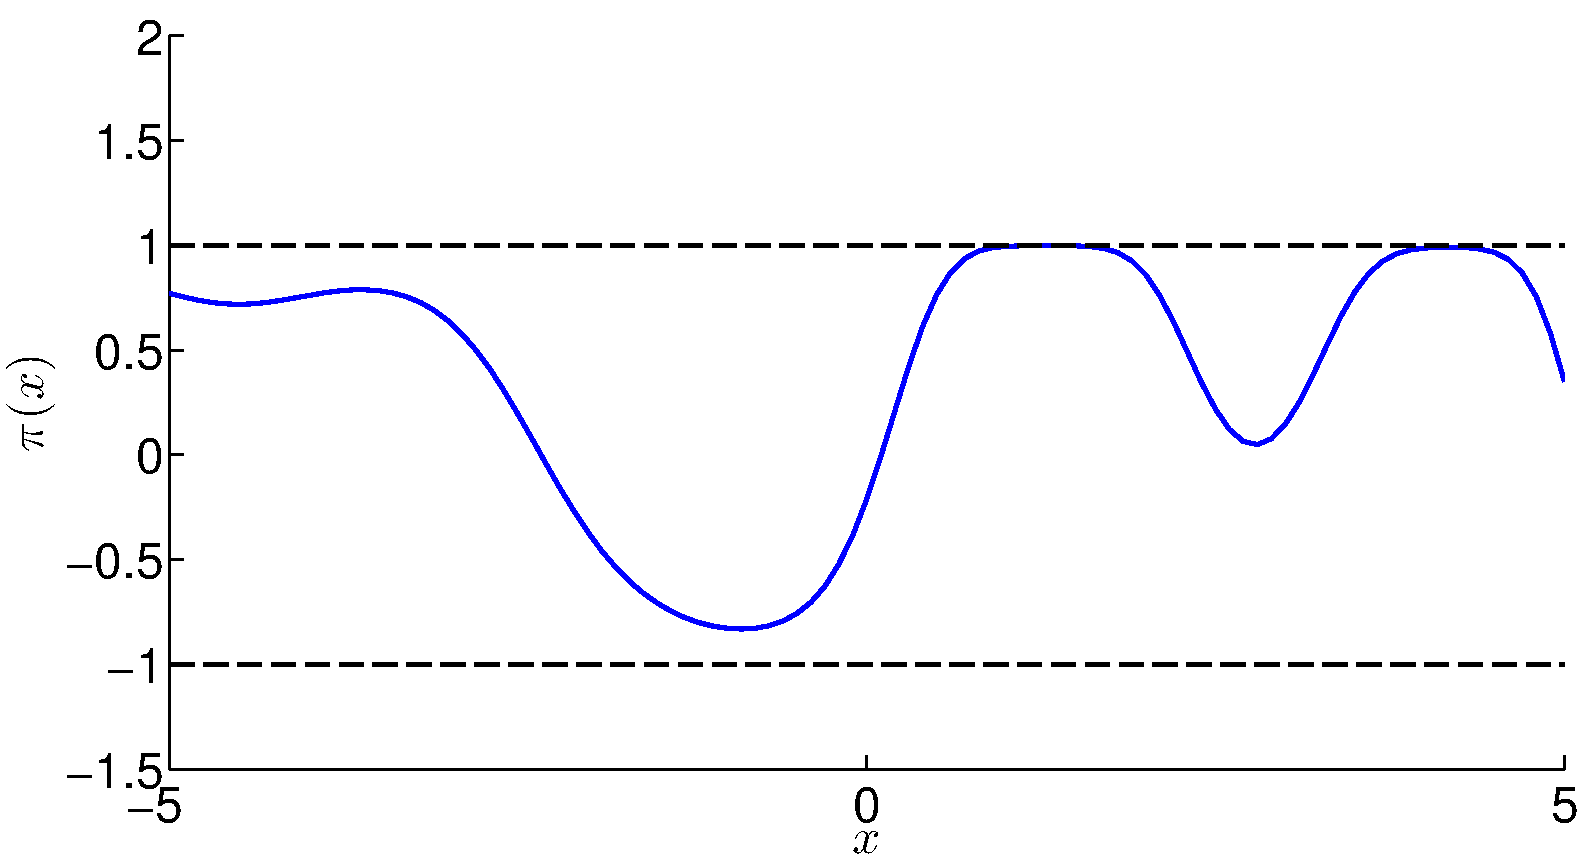
\includegraphics[width=0.45\hsize]{./figures/squashed_preliminary_policy}
\caption{Preliminary policy $\tilde\pi$ and squashed policy $\pi$. The
  squashing function ensures that the control signals $\vec u =
  \pi(\vec x)$ do not exceed the values $\pm \vec u_{\max}$.}
\end{figure}



\subsection{Plant Structure}
\begin{lstlisting}[name=settings_cp]
% 3. Plant structure
plant.dynamics = @dynamics_cp;                    % dynamics ode function
plant.noise = diag(ones(1,4)*0.01.^2);            % measurement noise
plant.dt = dt;
plant.ctrl = @zoh;                                % controler is zero order hold
plant.odei = odei;
plant.augi = augi;
plant.angi = angi;
plant.poli = poli;
plant.dyno = dyno;
plant.dyni = dyni;
plant.difi = difi;
plant.prop = @propagated;
\end{lstlisting}

\texttt{plant.dynamics} requires a function handle to the function
that implements the ODE for simulating the system.

\texttt{plant.noise} contains the measurement noise covariance
matrix. We assume the noise is zero-mean Gaussian. The noise is added
to the (latent) state during a trajectory rollout (see
\texttt{base/rollout.m}).

\texttt{plant.dt} is the sampling time, i.e., $1/dt$ is the sampling
frequency. 

\texttt{plant.ctrl} is the controller to be applied. Here,
\texttt{@zoh} implements a zero-order-hold controller. Other options
are \texttt{@foh} (first-order-hold) and \texttt{@lag}
(first-order-lag). For more information, have a look at
\texttt{base/simulate.m}.

\texttt{plant.odei}--\texttt{plant.difi} copy the indices defined
earlier into the \texttt{plant} structure.

\texttt{plant.prop} requires a function handle to the function that
computes $p(\vec x_{t+1})$ from $p(\vec x_t)$, i.e., a one-step
(probabilistic) prediction. In this software package, we implemented a
fairly generic function called \texttt{propagated}, which computes the
predictive state distribution $p(\vec x_{t+1})$ and the partial
derivatives that are required for gradient-based policy search. For
details about the gradients, we refer to~\cite{Deisenroth2011c}.



\subsection{Policy Structure}
\begin{lstlisting}[name=settings_cp]
% 4. Policy structure
policy.fcn = @(policy,m,s)conCat(@congp,@gSat,policy,m,s);% controller
                                                          % representation
policy.maxU = 10;                                         % max. amplitude of
                                                          % control
[mm ss cc] = gTrig(mu0, S0, plant.angi);                  % represent angles
mm = [mu0; mm]; cc = S0*cc; ss = [S0 cc; cc' ss];         % in complex plane
policy.p.inputs = gaussian(mm(poli), ss(poli,poli), nc)'; % init. location of
                                                          % basis functions
policy.p.targets = 0.1*randn(nc, length(policy.maxU));    % init. policy targets
                                                          % (close to zero)
policy.p.hyp = log([1 1 1 0.7 0.7 1 0.01])';              % initialize policy
                                                          % hyper-parameters
\end{lstlisting}
The policy we use in this example is the nonlinear policy given in
Equations~\eqref{eq:squashed rbf policy}--\eqref{eq:unsquashed rbf
  policy}. The policy function handle is stored in \texttt{policy.fcn}
(line 61).  In this particular example, the policy is a concatenation
of two functions: the RBF controller (\texttt{@congp}, see
\texttt{ctrl/congp.m}), which is parametrized as the mean of a GP with
a squared exponential covariance function, and a squashing function
$\sigma$ (\texttt{@gSat}, see \texttt{\path util/gSat.m}), defined as
%
\begin{align}
\sigma(x) = u_{\max}\frac{9\sin x+\sin (3x)}{8}\,,
\end{align}
% 
which is the third-order Fourier series expansion of a trapezoidal
wave, normalized to the interval \mbox{$[-u_{\max},-u_{\max}] $}.

\texttt{policy.maxU} (line 63) defines the maximum force value
$u_{\max}$ in Equation~\eqref{eq:squashed rbf policy}. We assume that
$u \in[-u_{\max},-u_{\max}]$.

% trigonometric augmentation
In lines 65--66, we augment the original state by $[\sin\theta,
\cos\theta]$ by means of \texttt{gTrig.m}, where the indices of the
angles $\theta$ are stored in \texttt{plant.angi}. We compute a
Gaussian approximation to the joint distribution $p(\vec x,
\sin\theta, \cos\theta)$. The representation of angles $\theta$ by
means of $[\sin\theta, \cos\theta]$ avoids discontinuities and
automatically takes care of the ``wrap-around condition'', i.e.,
$\theta \equiv \theta + 2k\pi, k \in\Z$.

The following lines are used to initialize the policy parameters. The
policy parameters are generally stored in \texttt{policy.p}. We
distinguish between three types of policy parameters:
\begin{itemize}
\item \texttt{policy.p.inputs}: These values play the role of the
  training inputs of a GP and correspond to the centers $\vec c_i$ of
  the policy in Equation~\eqref{eq:unsquashed rbf policy}. We sample
  the initial locations of the centers from the initial state
  distribution $p(\vec x_0)$. We compute this initial state
  distribution in lines 65--66, where we account for possible angle
  representations (\texttt{plant.angi}) of the state. If
  \texttt{plant.angi} is empty, lines 65--66 do not do anything and
  \texttt{mm}$=$\texttt{mu0} and \texttt{ss}$=$\texttt{S0}.
\item \texttt{policy.p.targets}: These values play the role of GP
  training targets are initialized to values close to zero.
\item \texttt{policy.p.hyp}: These values play the role of the GP
  log-hyper-parameters: log-length-scales,
  log-signal-standard-deviation, and log-noise-standard-deviation.  We
  initialize the policy hyper-parameters as follows:
\begin{itemize}
\item Length-scales: The length-scales weight the dimensions of the
  state that are passed to the policy (see \texttt{poli}). In our case
  these are: $x, \dot x, \dot\theta, \sin\theta, \cos\theta$.  We
  initialize the first three length-scales to 1. These values largely
  depend on the scale of the input data. In our example, the cart
  position and velocity are measured in $\unit{m}$ and $\unit{m/s}$,
  respectively, the angular velocity is measured in
  $\unit{rad/s}$. The last two length-scales scale trigonometric
  values, i.e., $\sin(\theta)$ and $\cos(\theta)$. Since these
  trigonometric functions map their argument into the interval
  $[-1,1]$, we choose a length-scale of 0.7, which is somewhat smaller
  than unity.
\item Signal variance: We set the signal variance of the controller
  $\tilde\pi$ to 1. Note that we squash $\tilde\pi$ through $\sigma$,
  see Equation~\eqref{eq:squashed rbf policy}. To exploit the full
  potential of the squashing function $\sigma$, it is sufficient to
  cover the domain $[-\pi/2,\pi/2]$. Therefore, we initialize the signal
  variance to 1.
\item Noise variance: The noise variance is only important only
  important as a relative factor to the signal variance. This ratio
  essentially determines how smooth the policy is. We initialize the
  noise variance to $0.01^2$.
\end{itemize}

\end{itemize}


\begin{figure}
\centering
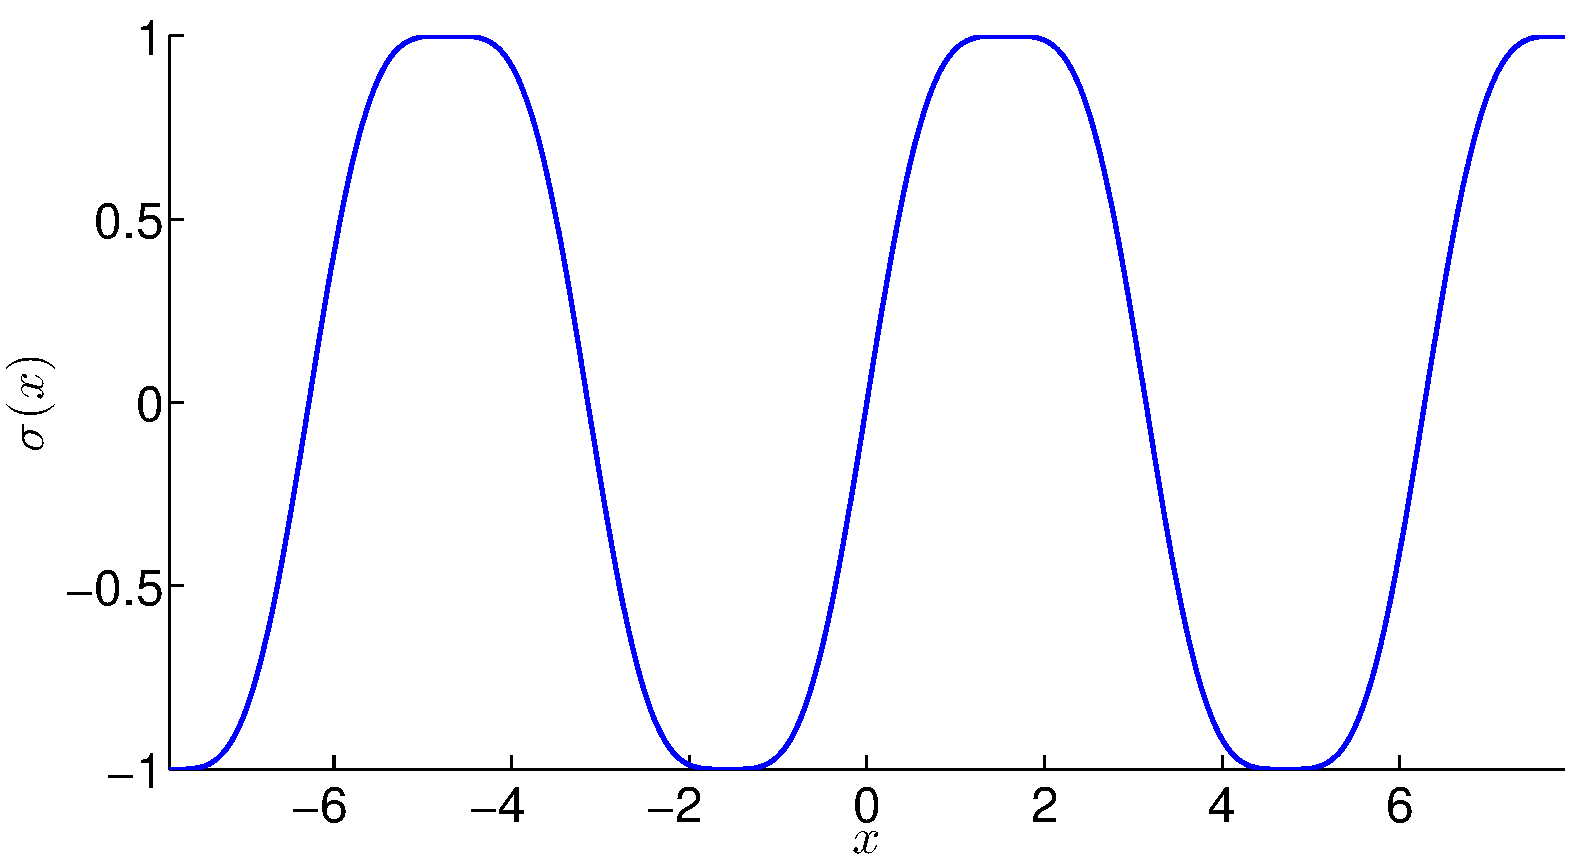
\includegraphics[ width = 0.4\hsize]{./figures/squashing_fct}
\hspace{5mm}
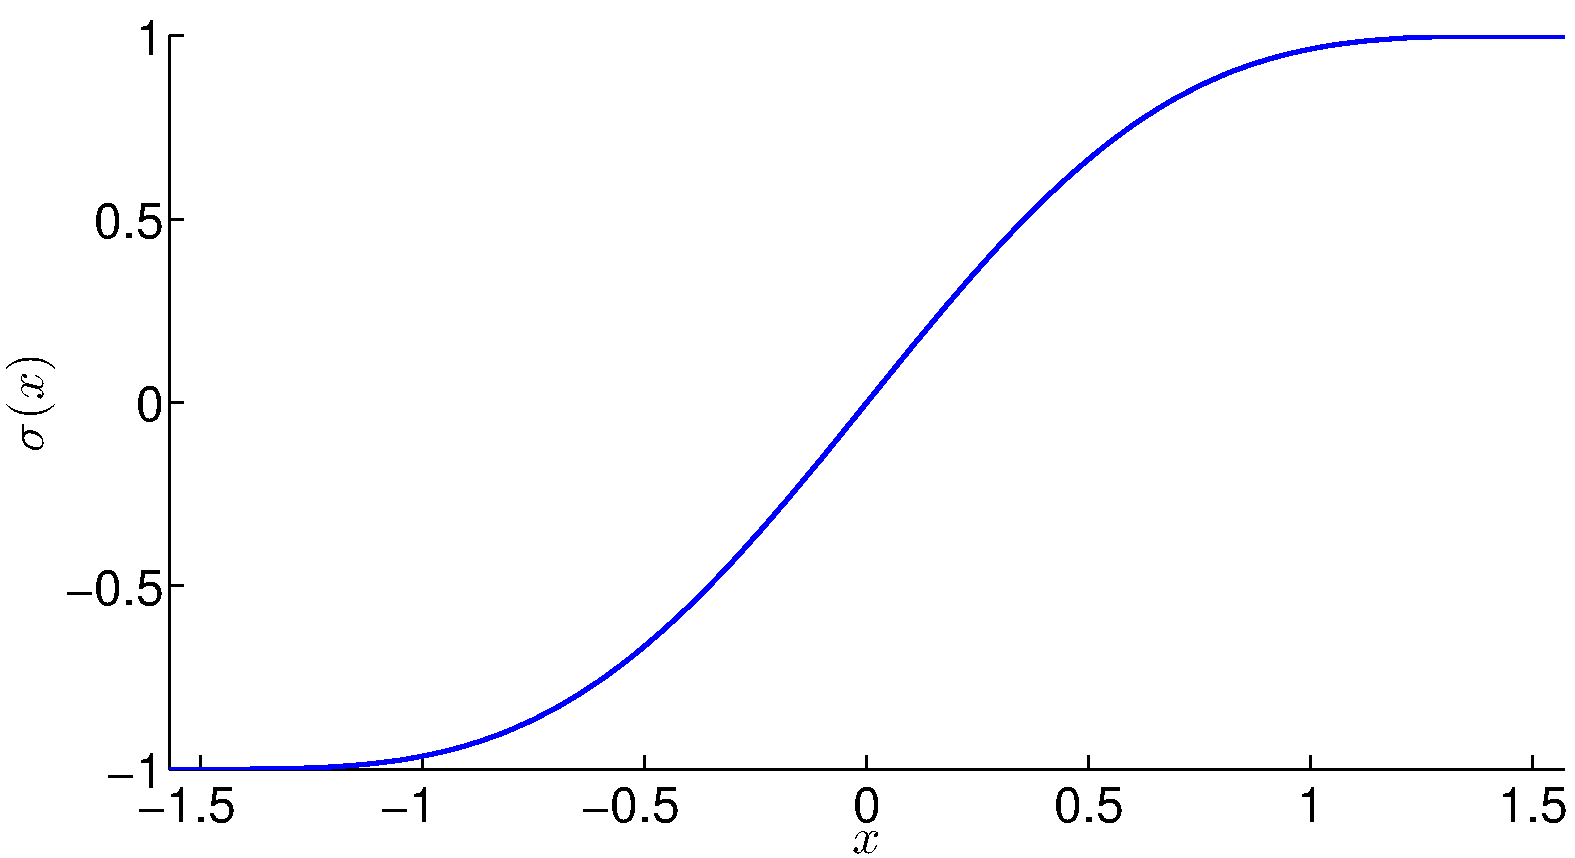
\includegraphics[width =
0.4\hsize]{./figures/squashing_fct2}
\caption{Squashing function.}
\end{figure}



\subsection{Cost Function Structure}
In the following, we set up a structure for the immediate cost
function.
\begin{lstlisting}[name=settings_cp]
% 5. Set up the cost structure
cost.fcn = @loss_cp;                       % cost function
cost.gamma = 1;                            % discount factor
cost.p = 0.5;                              % length of pendulum
cost.width = 0.25;                         % cost function width
cost.expl =  0.0;                          % exploration parameter (UCB)
cost.angle = plant.angi;                   % index of angle (for cost function)
cost.target = [0 0 0 pi]';                 % target state
\end{lstlisting}
%
In line 74, we store the function handle \texttt{@loss\_cp} in
\texttt{cost.fcn}. The function \texttt{loss\_cp} implements a
saturating cost function (an unnormalized Gaussian subtracted from 1)
with spread $\sigma_c$, i.e.,
%
\begin{align}
  c(\vec x) = 1 - \exp\big(-\tfrac{1}{2\sigma_c^2}\|\vec x - \vec
  x_{\text{target}}\|^2\big)\quad\in[0,1]
\label{eq:cp loss}
\end{align}
% 
where $\vec x_{\text{target}}$ is a target state.

We set the discount factor \texttt{cost.gamma} to 1 (line 75) as we
look at a finite-horizon problem.

The following parameters are specific to the cost function:
\begin{itemize}
\item \texttt{cost.p} (line 76) is the length of the pendulum. This
  length is needed to compute the Euclidean distance of the tip of the
  pendulum from the desired location in the inverted position.
\item \texttt{cost.width} (line 77) is the spread\slash width
  $\sigma_c$ of the cost function. Looking at the cost function in
  \eqref{eq:cp loss} and the target state $[x, \dot x, \dot\theta,
  \theta] = [0, *, *, 2k\pi+pi], k\in\Z$, the factor 0.25 essentially
  encodes that the pendulum has to be above horizontal, such that a
  cost substantially different from 1 is incurred (the length of the
  pendulum is $\unit[0.5]{m}$). Figure \ref{fig:loss sat cp}
  illustrates a simplified scenario with $\sigma_c = 1/2$.  For
  $c\approx 1$, it can get difficult to obtain any useful
  gradients. As a rule of thumb, one can set
  \texttt{cost.width}$=\|\vec\mu_0-\vec x_{\text{target}}\|/10$.
\item \texttt{cost.expl} (line 78) is a UCB-type exploration
  parameter. Negative values encourage exploration, positive values
  encourage the policy staying in regions with good predictive
  performance. We set the value to 0 in order to disable any kind of
  additional exploration or exploitation.
\item \texttt{cost.angle} (line 79) tells the cost function, which
  indices of the state are angles. In the cost function, we also
  represent angles in the complex plane.
\item \texttt{cost.target} (line 80) defines the target state $\vec
  x_{\text{target}}$. Here, the target state is defined as the cart
  being in the middle of the track and the pendulum upright, without
  any velocity or angular velocity. 
\end{itemize}

\begin{figure}[tb]
\centering
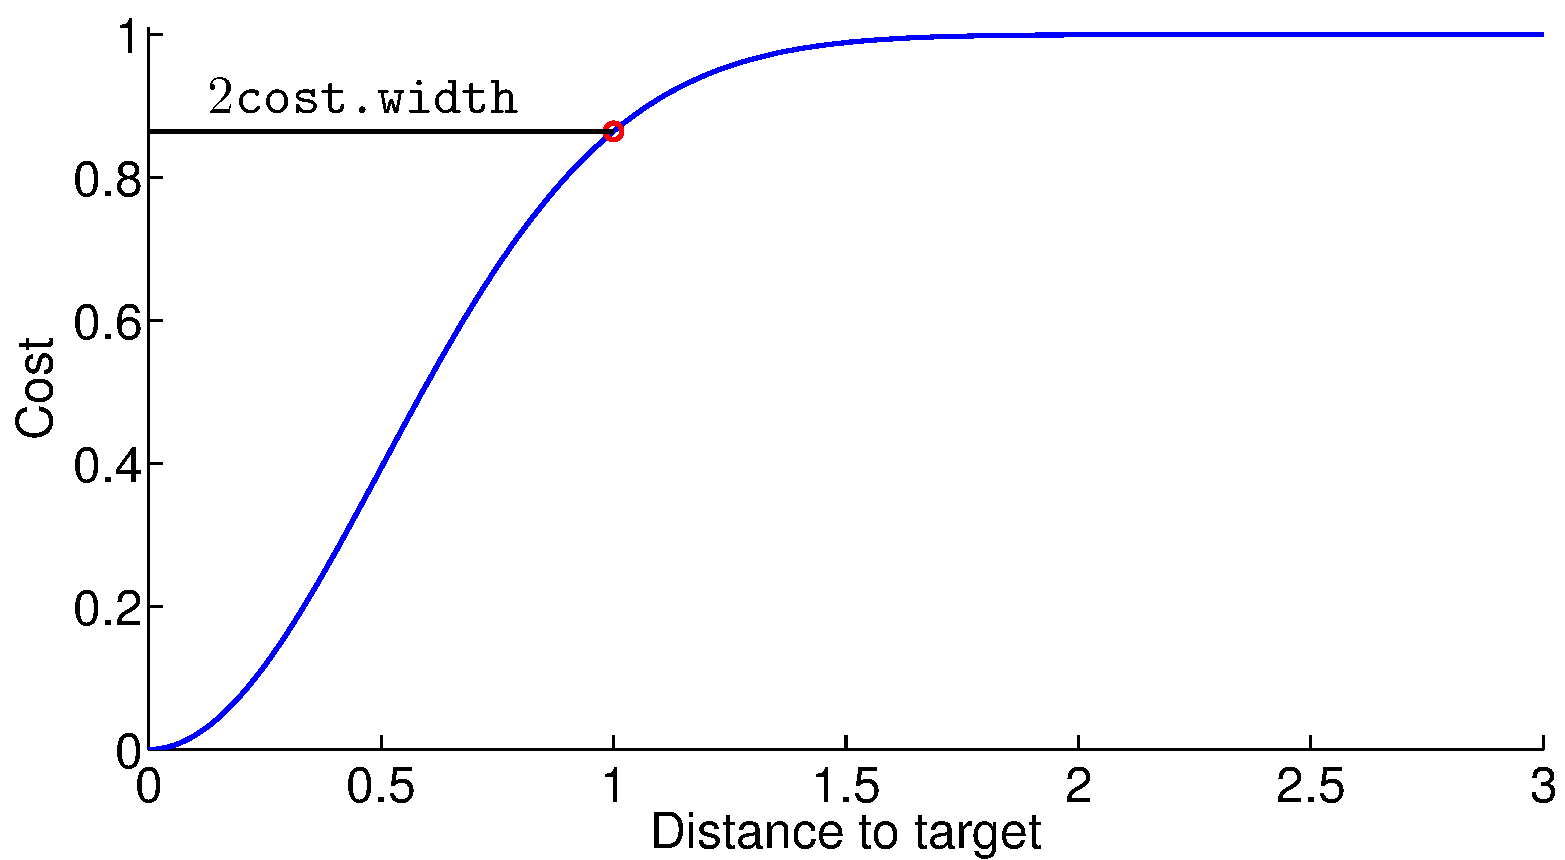
\includegraphics[width = 0.5\hsize]{./figures/satLossPlot}
\caption{In the saturating cost function, see Equation~\eqref{eq:cp
    loss}, \texttt{cost.width} determines determines how far away from
the target a cost $c<1$ can be attained.}
\label{fig:loss sat cp}
\end{figure}

\subsection{GP Dynamics Model Structure}
In the following, we set up the structure \texttt{dynmodel} for the GP
dynamics model.
%
\begin{lstlisting}[name=settings_cp]
% 6. Dynamics model structure
dynmodel.fcn = @gp1d;                % function for GP predictions
dynmodel.train = @train;             % function to train dynamics model
dynmodel.induce = zeros(300,0,1);    % shared inducing inputs (sparse GP)
trainOpt = [300 500];                % defines the max. number of line searches
                                     % when training the GP dynamics models
                                     % trainOpt(1): full GP,
                                     % trainOpt(2): sparse GP (FITC)
\end{lstlisting}
%
We generally assume that the model uses a squared exponential
covariance, a Gaussian likelihood, and a zero prior mean. Therefore,
these parameters are not explicitly specified here.

\texttt{dynmodel.fcn} (line 82) contains a function handle to
\texttt{gp1d}, which can predict with (sparse) GPs at uncertain
inputs. If the GP is not sparse but full, \texttt{gp1d} calls
\texttt{gp0d}, which implements GP predictions at uncertain inputs
with the full GP model. 

\texttt{dynmodel.train} (line 83) contains a function handle to
\texttt{train}, which is responsible for GP training.

\texttt{dynmodel.induce} (line 84) is optional and tells us when to
switch from full GPs to sparse GPs. \texttt{dynmodel.induce} is a
tensor of the form $a\times b\times c$, where $a$ is the number of
inducing inputs\footnote{If the size of the training set exceeds $a$,
  the full GP automatically switches to its sparse approximation.},
$b=0$ tells us that there are no inducing inputs yet, and $c$ is
either 1 or the number of predictive dimensions, which corresponds to
the number of indices stored in \texttt{dyno}. For $c=1$, the inducing
inputs are shared among all GPs. Otherwise, sets of inducing inputs
are separately learned for each predictive dimension.

\texttt{trainOpt} (line 85) contains the number of line searches for
GP hyper-parameter training used by the full GP (first number) and the
sparse GP (second parameter).

\subsection{Optimization Parameters (Policy Learning)}

In the following lines, we define (optional) parameters for policy
learning. Generally, we use an adapted version of
\texttt{minimize.m}\footnote{\url{http://www.gaussianprocess.org/gpml/code/matlab/util/minimize.m}},
a non-convex gradient-based optimizer. These optional parameters are
stored in a structure \texttt{opt}.
\begin{lstlisting}[name=settings_cp]
% 7. Parameters for policy optimization
opt.length = 150;                        % max. number of line searches
opt.MFEPLS = 30;                         % max. number of function evaluations
                                         % per line search
opt.verbosity = 1;                       % verbosity: specifies how much
                                         % information is displayed during
                                         % policy learning. Options: 0-3
\end{lstlisting}
\texttt{opt.length} (line 90) sets the maximum number of line searches after
which the optimizer returns the best parameter set so far. 

\texttt{opt.MFEPLS} (line 91) is the maximum number of function
evaluations per line search. Either the line search succeeds by
finding  a parameter set with a gradient close to 0 or it does not
succeed and aborts after \texttt{opt.MFEPLS} many function (and
gradient) evaluations. 

\texttt{opt.verbosity} (line 93) regulates the verbosity of the
optimization procedure. Verbosity ranges from 0 (no information
displayed) to 3 (visualize the line search and the computed
gradients\footnote{This is great for debugging.}).



\subsection{Plotting Parameters}
\begin{lstlisting}[name=settings_cp]
% 8. Plotting verbosity
plotting.verbosity = 1;            % 0: no plots
                                   % 1: some plots
                                   % 2: all plots
\end{lstlisting}
\texttt{plotting.verbosity} (line 97) is an easy way of controlling how much
information is visualized during policy learning. 



\subsection{Allocating Variables}
In lines 100-103, we simply initialize a few array that are used to
store data during the learning process.
\begin{lstlisting}[name=settings_cp]
% 9. Some initializations
x = []; y = [];
fantasy.mean = cell(1,N); fantasy.std = cell(1,N);
realCost = cell(1,N); M = cell(N,1); Sigma = cell(N,1);
\end{lstlisting}



\section{Cost Function}
In the following, we describe how to define a cost function for the
cart-pole swing-up scenario. The cost function is stored in
\texttt{loss\_cp.m} and implements the cost
%
\begin{align}
  c(\vec x) = \frac{1}{\#\texttt{cost.cw}}
  \sum_{i=1}^{\#\texttt{cost.cw}}(1-\exp\big(-\tfrac{1}{2(\sigma_c^{(i)})^2}\|\vec
  x-\vec x_{\text{target}}\|^2\big)
\label{eq:mixture cost}
\end{align}
% 
which is a generalized version of Equation~\eqref{eq:cp loss}. In
particular, \texttt{cost.cw} can be an array of different widths
$\sigma_c^{(i)}$, which is used to compute a cost function $c(\vec x)$ as a
mixture of cost functions with different widths.

%
The mean and the variance of the cost $c(\vec x)$ are computed by
averaging over the Gaussian state distribution $p(\vec x) = \mathcal
N(\vec x|\vec m,\mat S)$ with mean $\vec m$ and covariance matrix
$\mat S$. Derivatives of the expected cost and the cost variance with
respect to the mean and the covariance of the input distribution are
computed when desired. 

\subsection{Interface}
\begin{lstlisting}[name=loss_cp]
function [L, dLdm, dLds, S] = loss_cp(cost, m, s)
\end{lstlisting}
\begin{par}
\textbf{Input arguments:}
\end{par}\begin{verbatim}
cost            cost structure
  .p            length of pendulum                              [1 x  1 ]
  .width        array of widths of the cost (summed together)
  .expl         (optional) exploration parameter
  .angle        (optional) array of angle indices
  .target       target state                                    [D x  1 ]
m               mean of state distribution                      [D x  1 ]
s               covariance matrix for the state distribution    [D x  D ]\end{verbatim}
\begin{par}
\textbf{Output arguments:}
\end{par}
\begin{verbatim}
L     expected cost                                             [1 x  1 ]
dLdm  derivative of expected cost wrt. state mean vector        [1 x  D ]
dLds  derivative of expected cost wrt. state covariance matrix  [1 x D^2]
S     variance of cost                                          [1 x  1 ]
\end{verbatim}






\begin{lstlisting}[name=loss_cp]
if isfield(cost,'width'); cw = cost.width; else cw = 1; end
if ~isfield(cost,'expl') || isempty(cost.expl); b = 0; else b =  cost.expl; end
\end{lstlisting}
In lines 2--3, we check whether a scaling factor (array) and an
exploration parameter exist. Default values are 1 (no scaling) and 0
(no exploration), respectively.




\begin{lstlisting}[name=loss_cp]
% 1. Some precomputations
D0 = size(s,2);                           % state dimension
D1 = D0 + 2*length(cost.angle);           % state dimension (with sin/cos)

M = zeros(D1,1); M(1:D0) = m; S = zeros(D1); S(1:D0,1:D0) = s;
Mdm = [eye(D0); zeros(D1-D0,D0)]; Sdm = zeros(D1*D1,D0);
Mds = zeros(D1,D0*D0); Sds = kron(Mdm,Mdm);
\end{lstlisting}
In line 5, the dimension of the state is determined.

In line 6, the dimension of the state is augmented to account for
potential angles in the state, which require a representation on the
unit circle via $\sin\theta$ and $\cos\theta$. Therefore, the (fully)
augmented state variable is then given as
%
\begin{align}
  \vec j = [x, \dot x, \dot\theta, \theta, \sin\theta,
  \cos\theta]\T\,.
\label{eq:aug state}
\end{align}
% 

Lines 8--10 initialize the output arguments to 0.


In the following lines, the distance $\vec x-\vec x_{\text{target}}$
is computed.
\begin{lstlisting}[name=loss_cp]
% 2. Define static penalty as distance from target setpoint
ell = cost.p; % pendulum length
Q = zeros(D1); Q([1 D0+1],[1 D0+1]) = [1 ell]'*[1 ell]; Q(D0+2,D0+2) = ell^2;
\end{lstlisting}
%
Line 12 stores the pendulum length in \texttt{ell}.

In line 12, the matrix $\mat Q$ is computed, such that $(\vec j - \vec
j_{\text{target}})\T\mat Q (\vec j - \vec
j_{\text{target}})$ is the squared Euclidean distance between the tip
of the pendulum in the current state and the target state. For $\vec
x_{\text{target}} = [0, *, *, \pi]\T$, i.e., the pendulum is balanced
in the inverted position in the middle of the track, the Euclidean
distance is given as
\begin{align}
  \|\vec x -\vec x_{\text{target}}\|^2
  &=x^2+2xl\sin\theta+2l^2+2l^2\cos\theta = (\vec j - \vec
  j_{\text{target}})\T\mat Q (\vec j - \vec
  j_{\text{target}})\,,\\
  \mat Q &= \begin{bmatrix}
    1& 0 &0 & 0 & l&0\\
    0& 0 &0 & 0 & 0 &0\\
    0& 0 &0 & 0 & 0 &0\\
    0& 0 &0 & 0 & 0 &0\\
    l&  0 &0 & 0 & l^2&0\\
    0&  0 &0 & 0&  0&l^2
\end{bmatrix}\,.
\end{align}
Note that at this point only the $\mat Q$-matrix is determined.


\begin{lstlisting}[name=loss_cp]
% 3. Trigonometric augmentation
if D1-D0 > 0
  % augment target
  target = [cost.target(:); gTrig(cost.target(:), 0*s, cost.angle)];

  % augment state
  i = 1:D0; k = D0+1:D1;
  [M(k) S(k,k) C mdm sdm Cdm mds sds Cds] = gTrig(M(i),S(i,i),cost.angle);

  % compute derivatives (for augmentation)
  X = reshape(1:D1*D1,[D1 D1]); XT = X';              % vectorized indices
  I=0*X; I(i,i)=1; ii=X(I==1)'; I=0*X; I(k,k)=1; kk=X(I==1)';
  I=0*X; I(i,k)=1; ik=X(I==1)'; ki=XT(I==1)';

  Mdm(k,:)  = mdm*Mdm(i,:) + mds*Sdm(ii,:);                    % chainrule
  Mds(k,:)  = mdm*Mds(i,:) + mds*Sds(ii,:);
  Sdm(kk,:) = sdm*Mdm(i,:) + sds*Sdm(ii,:);
  Sds(kk,:) = sdm*Mds(i,:) + sds*Sds(ii,:);
  dCdm      = Cdm*Mdm(i,:) + Cds*Sdm(ii,:);
  dCds      = Cdm*Mds(i,:) + Cds*Sds(ii,:);

  S(i,k) = S(i,i)*C; S(k,i) = S(i,k)';                      % off-diagonal
  SS = kron(eye(length(k)),S(i,i)); CC = kron(C',eye(length(i)));
  Sdm(ik,:) = SS*dCdm + CC*Sdm(ii,:); Sdm(ki,:) = Sdm(ik,:);
  Sds(ik,:) = SS*dCds + CC*Sds(ii,:); Sds(ki,:) = Sds(ik,:);
end
\end{lstlisting}
This block is only executed if angles are present (the check is
performed in line 15).

First (line 17), the target state $\vec x_{\text{target}}$ is
augmented to 
$$\vec j_{\text{target}} = [x_{\text{target}},\dot
x_{\text{target}}, \dot\theta_{\text{target}}, \theta_{\text{target}},
\sin(\theta_{\text{target}}),\cos(\theta_{\text{target}})]\T\,.$$

In line 21, the state distribution $p(\vec x)$ is probabilistically
augmented to $p(\vec j)$, where $\vec j$ is given in
Equation~\eqref{eq:aux state}. Note that $p(\vec j)$ cannot be
computed analytically. Instead, we compute the mean and covariance of
$p(\vec j)$ exactly and approximate $p(\vec j)$ by a Gaussian. This
probabilistic augmentation and the corresponding derivatives with
respect to the mean and covariance of the state distribution are
computed by \texttt{\path util/gTrig.m}.

Lines 28--38 compute the derivatives of the mean and covariance of
$p(\vec j)$ and the cross-covariance $\cov[\vec x, \vec j]$ with
respect to the mean and covariance of $p(\vec x)$ using the chain
rule.


\begin{lstlisting}[name=loss_cp]
% 4. Calculate loss
L = 0; dLdm = zeros(1,D0); dLds = zeros(1,D0*D0); S = 0;
for i = 1:length(cw)                    % scale mixture of immediate costs
  cost.z = target; cost.W = Q/cw(i)^2;
  [r rdM rdS s2 s2dM s2dS] = lossSat(cost, M, S);

  L = L + r; S  = S + s2;
  dLdm = dLdm + rdM(:)'*Mdm + rdS(:)'*Sdm;
  dLds = dLds + rdM(:)'*Mds + rdS(:)'*Sds;

  if (b~=0 || ~isempty(b)) && abs(s2)>1e-12
    L = L + b*sqrt(s2);
    dLdm = dLdm + b/sqrt(s2) * ( s2dM(:)'*Mdm + s2dS(:)'*Sdm )/2;
    dLds = dLds + b/sqrt(s2) * ( s2dM(:)'*Mds + s2dS(:)'*Sds )/2;
  end
end

% normalize
n = length(cw); L = L/n; dLdm = dLdm/n; dLds = dLds/n; S = S/n;
\end{lstlisting}
After all the pre-computations, in lines 40--58, the expected cost for
Equation~\eqref{eq:mixture cost} is finally computed:

For all widths of the cost structure (line 42), we compute the mean
and the variance of the saturating cost in Equation~\eqref{eq:cp
  loss}, including the derivatives with respect to the mean and the
covariance of $p(\vec j)$, see line 44. For these computations, the
function \texttt{loss/lossSat.m} is called. 

Lines 47--48 compute the derivatives of the expected cost and the
variance of the cost with respect to the mean and covariance matrix of
the state distribution $p(\vec x)$ by applying the chain rule.

If exploration is desired (line 50), we add $\kappa\sqrt{\var[c(\vec
  x)]}$ to the $\E[c(\vec x)]$ to allow for UCB-type exploration, see
Equation~\eqref{eq:UCB cost}


\section{Visualization}

The following lines of code display a sequence of images (video) of a
cart-pole trajectory and can be found in \texttt{\path
  scenarios/cartPole/draw\_rollout\_cp.m}.
\begin{lstlisting}
% Loop over states in trajectory (= time steps)
for r = 1:size(xx,1)
  if exist('j','var') && ~isempty(M{j})
    draw_cp(latent{j}(r,1), latent{j}(r,4), latent{j}(r,end), cost,  ...
      ['trial # ' num2str(j+J) ', T=' num2str(H*dt) ' sec'], ...
      ['total experience (after this trial): ' num2str(dt*size(x,1)) ...
      ' sec'], M{j}(:,r), Sigma{j}(:,:,r));
  else
     draw_cp(latent{jj}(r,1), latent{jj}(r,4), latent{jj}(r,end), cost,  ...
      ['(random) trial # ' num2str(jj) ', T=' num2str(H*dt) ' sec'], ...
      ['total experience (after this trial): ' num2str(dt*size(x,1)) ...
      ' sec'])
  end
  pause(dt);
end
\end{lstlisting}
At each time step \texttt{r} of the most recent trajectory (stored in
\texttt{xx}), an image of the current cart-pole state is drawn by
repeatedly calling \texttt{draw\_cp}. We distinguish between two modes
(\texttt{if-else} statement): Either we draw a trajectory \emph{after}
having learned a policy (\texttt{if} statement), or we draw a
trajectory from a random rollout, i.e., before a policy is learned
(\texttt{else} statement). In the first case, \texttt{draw\_cp} also
visualizes the long-term predictive means and variances of the tip of
the pendulum, which are not given otherwise.

% draw_cp
The \texttt{draw\_cp} function plots the cart-pole system with reward,
applied force, and predictive uncertainty of the tip of the
pendulum. We just describe the interface in the following. The code is
available at \texttt{\path scenarios/cartPole/draw\_cp.m}.


\begin{lstlisting}
function draw_cp(x, theta, force, cost, text1, text2, M, S)
\end{lstlisting}

    \begin{par}
\textbf{Input arguments:}
\end{par} \vspace{1em}

\begin{verbatim}
  x          position of the cart
  theta      angle of pendulum
  force      force applied to cart
  cost       cost structure
    .fcn     function handle (it is assumed to use saturating cost)
    .<>      other fields that are passed to cost
  M          (optional) mean of state
  S          (optional) covariance of state
  text1      (optional) text field 1
  text2      (optional) text field 2
\end{verbatim}




\section{Main Function} 
 
The main function executes the following high-level steps.
\begin{enumerate}
   \item Load scenario-specific setting
   \item Create \texttt{J} initial trajectories by applying random controls
   \item Controlled learning:
\begin{enumerate}
\item Train dynamics model
\item Learn policy
\item Apply policy to system
\end{enumerate}
\end{enumerate}


\begin{lstlisting}[name=cpmain]
% 1. Initialization
clear all; close all;
settings_cp;                      % load scenario-specific settings
basename = 'cartPole_';           % filename used for saving data
\end{lstlisting}
Lines 1--4 load scenario-specific settings (line 3) and define a
basename for data that is stored throughout the execution.


\begin{lstlisting}[name=cpmain]
% 2. Initial J random rollouts
for jj = 1:J
  [xx, yy, realCost{jj}, latent{jj}] = ...
    rollout(gaussian(mu0, S0), struct('maxU',policy.maxU), H, plant, cost);
  x = [x; xx]; y = [y; yy];       % augment training sets for dynamics model
  if plotting.verbosity > 0;      % visualization of trajectory
    if ~ishandle(1); figure(1); else set(0,'CurrentFigure',1); end; clf(1);
    draw_rollout_cp;
  end

end

mu0Sim(odei,:) = mu0; S0Sim(odei,odei) = S0;
mu0Sim = mu0Sim(dyno); S0Sim = S0Sim(dyno,dyno);
\end{lstlisting}
To kick off learning, we need to create an initial (small) data set
that can be learned for learning the first GP dynamics model. For
this, we generate \texttt{J} trajectories of length \texttt{H} by
applying random control signals using \texttt{\path base/rollout.m},
(lines 7--8). Generally, the training data for the GP is stored in
\texttt{x} and \texttt{y} (line 9). If desired, the trajectories of
the cart-pole system are visualized (lines 10--13).
%
In lines 17--18, we define variables \texttt{mu0Sim} and
\texttt{S0Sim}, which are used subsequently.



\begin{lstlisting}[name=cpmain]
% 3. Controlled learning (N iterations)
for j = 1:N
  trainDynModel;   % train (GP) dynamics model
  learnPolicy;     % learn policy
  applyController; % apply controller to system
  disp(['controlled trial # ' num2str(j)]);
  if plotting.verbosity > 0;      % visualization of trajectory
    if ~ishandle(1); figure(1); else set(0,'CurrentFigure',1); end; clf(1);
    draw_rollout_cp;
  end
end
\end{lstlisting}
The actual learning happens in lines 19--29, where \textsc{pilco}
performs \texttt{N} (controlled) iterations of dynamics model learning
(line 21), policy search (line 22), and controller application to the
system (line 23). If desired, the trajectories of
the cart-pole system are visualized (lines 25--28). 


\subsection{Screen Prints and Visualization}

When training the GP dynamics model, a typical feedback in the command
window looks as follows:\\
\line(1,0){400}
\begin{verbatim}
Train hyper-parameters of full GP ...
GP 1/4
Initial Function Value 1.853671e+01
linesearch #     31;  value -8.942969e+01
GP 2/4
Initial Function Value 3.115190e+01
linesearch #     34;  value -4.210842e+01
GP 3/4
Initial Function Value 8.045295e+01
linesearch #     30;  value 4.742728e+00
GP 4/4
Initial Function Value -3.771471e+00
linesearch #     37;  value -6.971879e+01
Learned noise std: 0.016818    0.016432     0.04385    0.019182
SNRs             : 28.91172      116.4612      112.2714      49.12984
\end{verbatim}
\line(1,0){400}\\
%
In this cart-pole example, we train four GPs (one for each predictive
dimension stored in \texttt{dyno}). The hyper-parameters are learned
after 30--40 line searches. Positive values are generally and
indicator that the learned model is not so good at predicting this
target dimension. This might be due to sparse data and\slash or very
nonlinear dynamics. At the end, the learned noise standard deviations
are displayed, together with the signal-to-noise ratios (SNRs). The
SNRs are computed as 
%
\begin{align*}
SNR = \frac{\sqrt{\sigma_f^2}}{\sqrt{\sigma_{\text{noise}}^2}}\,,
\end{align*}
% 
where $\sigma_f^2$ is the variance of the underlying function and
$\sigma_{\text{noise}}^2$ is the inferred noise variance. High SNRs
($>$ 500) are penalized during GP training in \texttt{\path
  gp/hypCurb.m} to improve numerical stability. If there are SNRs
$>500$, it might be worthwhile adding some more noise to the GP
training targets.



%%%%%%%%% policy optimization


\begin{figure}
\centering
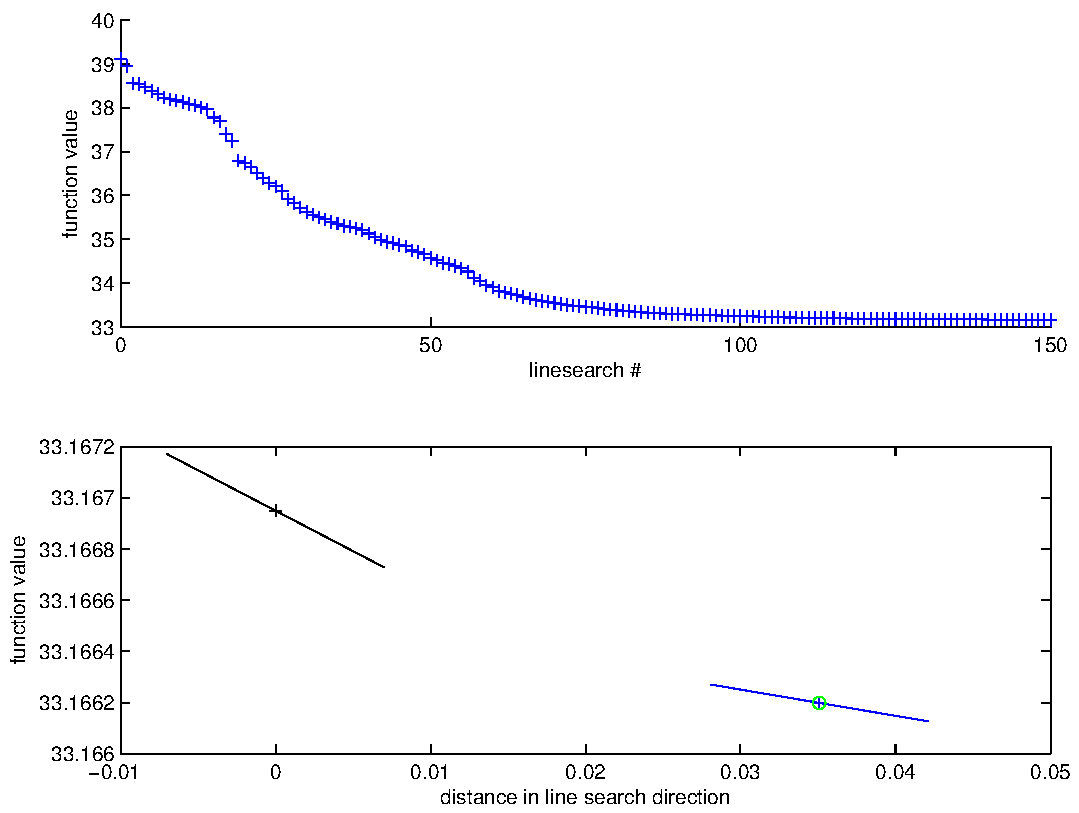
\includegraphics[width = 0.7\hsize]{./figures/policy_opt}
\caption{Typical display during policy learning: The top subplot shows
  the overall progress of policy learning as a function of the number
  of line searches. In this example, the initial policy caused a total
  expected cost $J(\vec \theta)$ of 39.11; the policy after 150 line
  search searches caused an expected cost of 33.16. The bottom subplot
  shows the progress of the current line search as a function of the
  distance in line search direction. The function values (+) and the
  corresponding gradients are visualized. For more detailed
  information about the visualization and the verbosity of the output
  (\texttt{opt.verbosity}), we refer to \texttt{\path
    util/minimize.m}.}
\label{fig:policy optimization}
\end{figure} 
% 
Figure~\ref{fig:policy optimization} displays a typical screen output
during policy optimization, showing the overall progress of policy
learning (top subplot) and the progress of the current line search
(bottom subplot). The following lines are simultaneously displayed in
the command window to show the current progress of learning:
%
\\\line(1,0){400}
\begin{verbatim}
Initial Function Value 3.910902e+01
linesearch #    150;  value 3.316620e+01
\end{verbatim}
\line(1,0){400}\\
If \texttt{opt.verbosity}$<3$, i.e., we are not interested in
permanently displaying the gradients as in Figure~\ref{fig:policy
  optimization}, it is possible to display the overall optimization
progress at the end of each policy search by setting
\texttt{plotting.verbosity=2}. The corresponding figure is given in
Figure~\ref{fig:fX3}. 
%
\begin{figure}[tb]
\centering
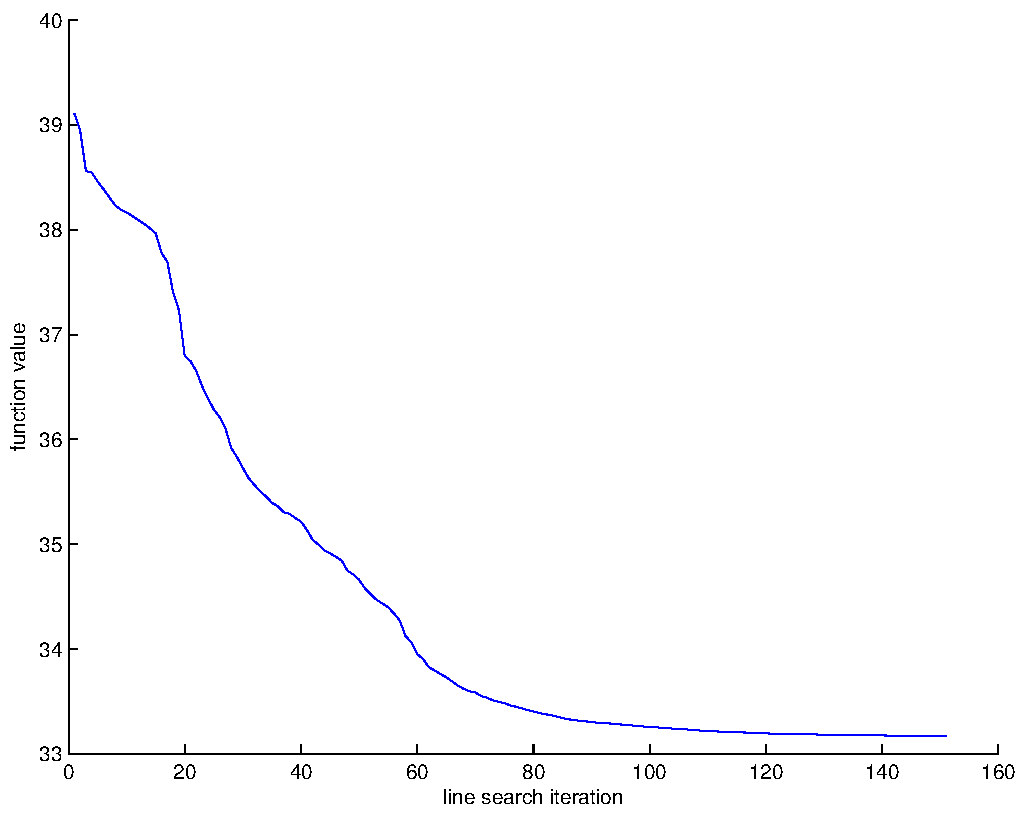
\includegraphics[width = 0.6\hsize]{./figures/fX3}
\caption{Overall progress of a policy search with 150 line searches.}
\label{fig:fX3}
\end{figure}
% 
This figure visually indicates whether the policy search was close to
convergence. If it frequently happens that the curve does not flatten
out, it might be worthwhile increasing the value of
\texttt{opt.length} in the scenario-specific settings file (here:
\texttt{settings\_cp.m}).

%
\begin{figure}[tb]
\centering
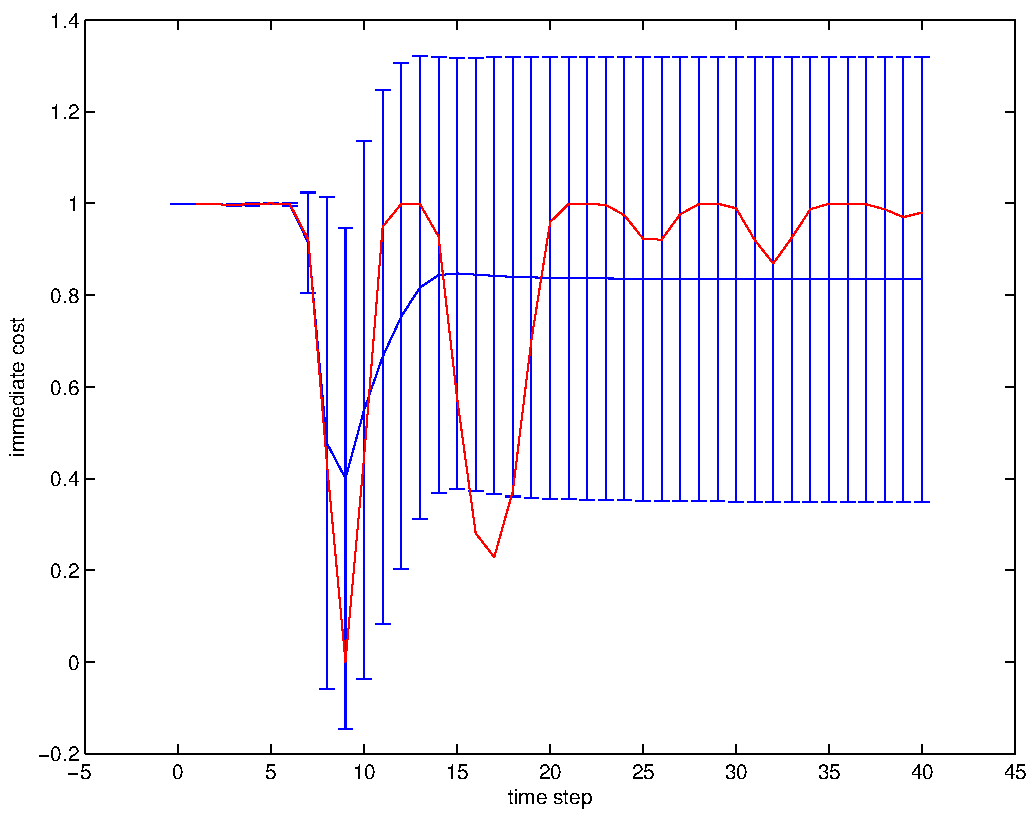
\includegraphics[width = 0.6\hsize]{./figures/cost_error_bar}
\caption{Predicted immediate cost (blue error bar) and corresponding
  incurred cost when applying the policy (red) for each time step of
  the prediction horizon.}
\label{fig:cost error bar}
\end{figure}
%
Figure~\ref{fig:cost error bar} shows the predicted and the incurred
immediate cost when applying the policy. Initially, the cost is at
unity, which means that the initial state is far from the target
area. After around 6 time steps, the predictive uncertainty in the
cost increases, which means that the predictive state distribution
substantially overlaps with the target area. In Figure~\ref{fig:cost
  error bar} the reason is that the predictive state increases very
quickly during the first time steps. 


\begin{figure}[tb]
\centering
\subfigure[Early stages of learning.]{
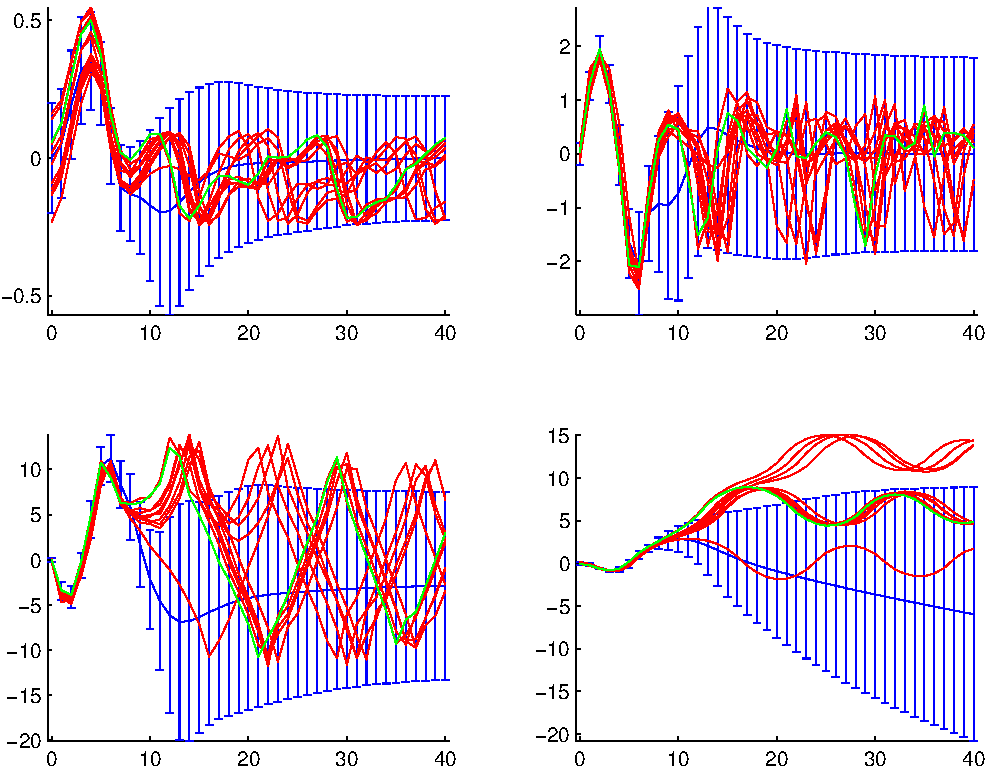
\includegraphics[width = 0.48\hsize]{./figures/example_trajectories}
\label{fig:example trajectories early}
}
\hfill
\subfigure[Final stages of learning.]{
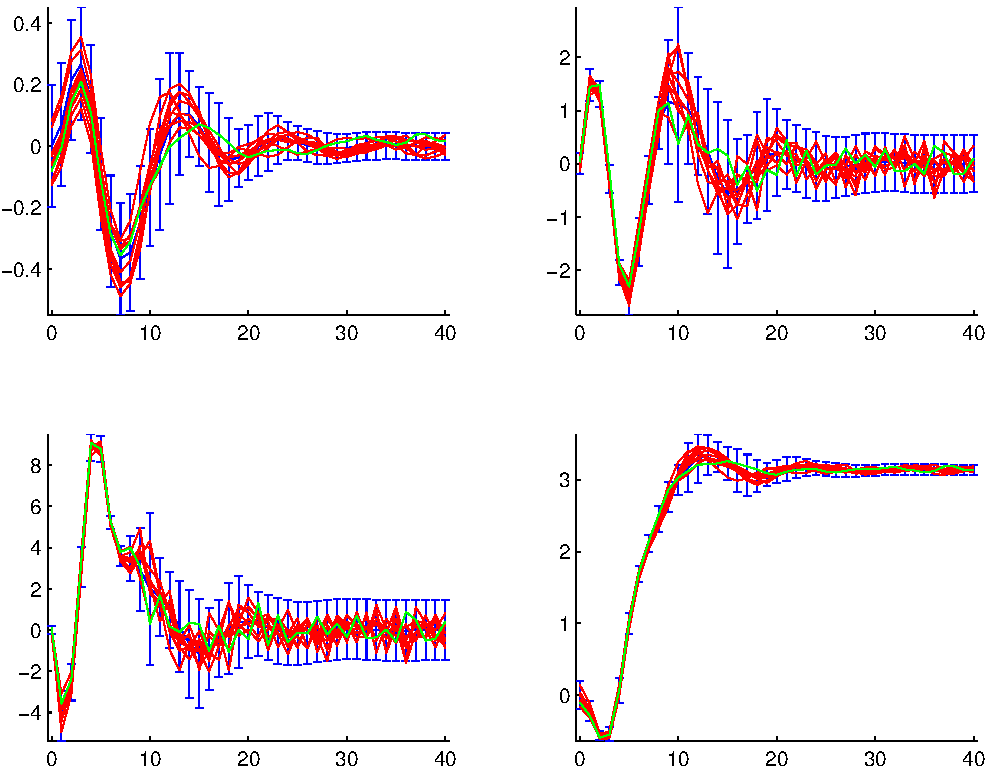
\includegraphics[width = 0.48\hsize]{./figures/example_trajectories2}
\label{fig:example trajectories final}
}
\caption{Example trajectories. For each predictive dimension
  (\texttt{dyno}), ten state trajectories are displayed, which
  occurred when the same policy $\pi(\vec\theta^*)$ is applied to the
  system. Note that the initial state differs as it is sampled from
  the start state distribution, i.e., $\vec x_0\sim p(\vec x_0)$. The
  green trajectory will be used in the next learning iteration to
  update the GP training set; the other (red) trajectories are
  generated to get an impression of the quality of the long-term
  predictive state distributions, the 95\% confidence intervals of
  which are shown by the blue error bars.}
\label{fig:example trajectories}
\end{figure}
%
Figure~\ref{fig:example trajectories} shows two sets of example
trajectories for each predictive dimension. One set is generated in
the early stages of learning (Figure~\ref{fig:example trajectories
  early}), the other one is generated in the final stages of learning
(Figure~\ref{fig:example trajectories final}). The green trajectory is
stored in \texttt{xx} and will be used to augment the training data
set for the GP model. The red trajectories are generated to (a)
indicate whether the green trajectory is a ``typical'' trajectory or
an outlier, (b) show the quality of the long-term predictive state
distributions, whose 95\% predictive confidence intervals are
indicated by the blue error bars, (c) give an intuition how sensitive
the currently learned controller is to different initial states $\vec
x_0\sim p(\vec x_0)$. As shown in Figure~\ref{fig:example trajectories
  early}, in the early stages of learning, the controller is very
sensitive to the initial conditions, i.e., the controlled trajectories
vary a lot. A good controller is robust to the uncertain initial
conditions and leads to very similar controlled trajectories as shown
in Figure~\ref{fig:example trajectories final}.


\begin{figure}[tb]
\centering
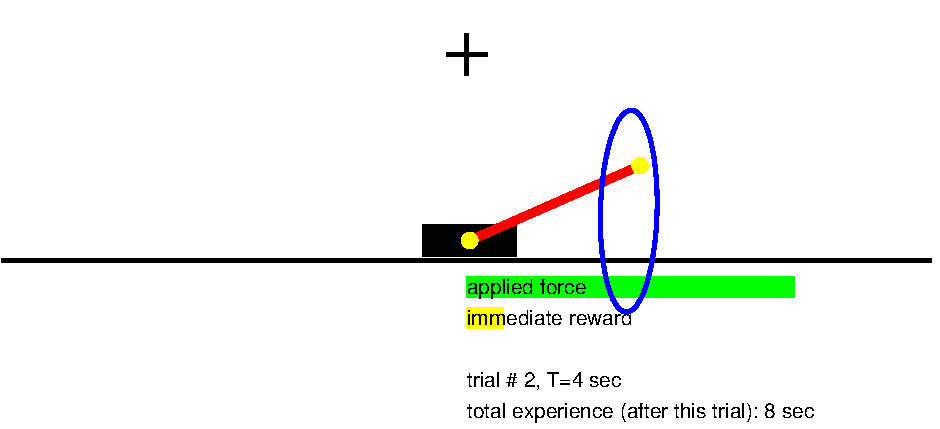
\includegraphics[width=0.6\hsize]{./figures/cp_rollout}
\caption{Visualization of a trajectory of the cart-pole swing-up
  during learning. The cart runs on an (infinite) track, the pendulum
  is freely swinging. The cross denotes the target location for
  balancing the tip of the pendulum, and the blue ellipse represents
  the 95\% confidence bound of a $t$-step ahead prediction of the
  location of the tip of the pendulum when applying the learned
  policy. We also display the applied force (green bar), whose values
  $u_{\max}$ and $-u_{\max}$ correspond to a green bar being either
  full to the right or left side. Here, ``full'' means at the end of
  the black line that represents the track. Moreover, we show the
  incurred immediate reward (negative cost) of the current state of
  the system. The immediate reward is represented by a yellow bar,
  whose maximum is at the right end of the black bar. We also display
  the number of total trials (this includes the random initial
  trials), the prediction horizon $T$, and the total experience after
  this trial.}
\label{fig:cp rollout}
\end{figure}
%
Figure~\ref{fig:cp rollout} shows a snapshot of a visualization of a
trajectory of the cart-pole system. The cart runs on an (infinite)
track, the pendulum is freely swinging. The cross denotes the target
location for balancing the tip of the pendulum, and the blue ellipse
represents the 95\% confidence bound of a $t$-step ahead prediction of
the location of the tip of the pendulum when applying the learned
policy. We also display the applied force (green bar), whose values
$u_{\max}$ and $-u_{\max}$ correspond to a green bar being either full
to the right or left side. Here, ``full'' means at the end of the
black line that represents the track. Moreover, we show the incurred
immediate reward (negative cost) of the current state of the
system. The immediate reward is represented by a yellow bar, whose
maximum is at the right end of the black bar. We also display the
number of total trials (this includes the random initial trials), the
prediction horizon $T$, and the total experience after this trial.

\begin{table}
\centering
\caption{\texttt{plotting.verbosity} Overview.}
\begin{tabular}{l || cccc}
& 
Figure~\ref{fig:fX3} & Figure~\ref{fig:cost error bar} &
Figure~\ref{fig:example trajectories} & Figure~\ref{fig:cp rollout}\\
\hline
\texttt{plotting.verbosity=0}  & \xmark &\xmark &\xmark & \xmark \\
\texttt{plotting.verbosity=1}  & \xmark &\cmark &\xmark & \cmark \\
\texttt{plotting.verbosity=2}  & \cmark &\cmark &\cmark & \cmark
\end{tabular}
\end{table}



\chapter{Implemented Scenarios}

In the following, we introduce the scenarios that are shipped with
this software package, and detail the derivation of the corresponding
equations of motion, taken from~\cite{Deisenroth2010b}. All
scenarios have their own folder in \texttt{\path scenarios/}.

\begin{table}[ht]
  \caption{State and control space dimensions in the implemented
    scenarios.}
\label{tab:scenarios}
\centering
\begin{tabular}{c||cc}
Task & State Space & Control Space\\
\hline
Pendulum & $\R^2$ & $\R$\\
Pendubot & $\R^4$ & $\R$\\
Double Pendulum &  $\R^4$ & $\R^2$\\
Cart-Pole & $\R^4$ & $\R$\\
Cart-Double Pendulum & $\R^6$ & $\R$\\
Unicycling & $\R^{12}$ & $\R^2$
\end{tabular}
\end{table}
%
Table~\ref{tab:scenarios} gives an
overview of the corresponding state and control dimensions.


\section{Pendulum Swing-up}
\begin{figure}[tb]
\centering
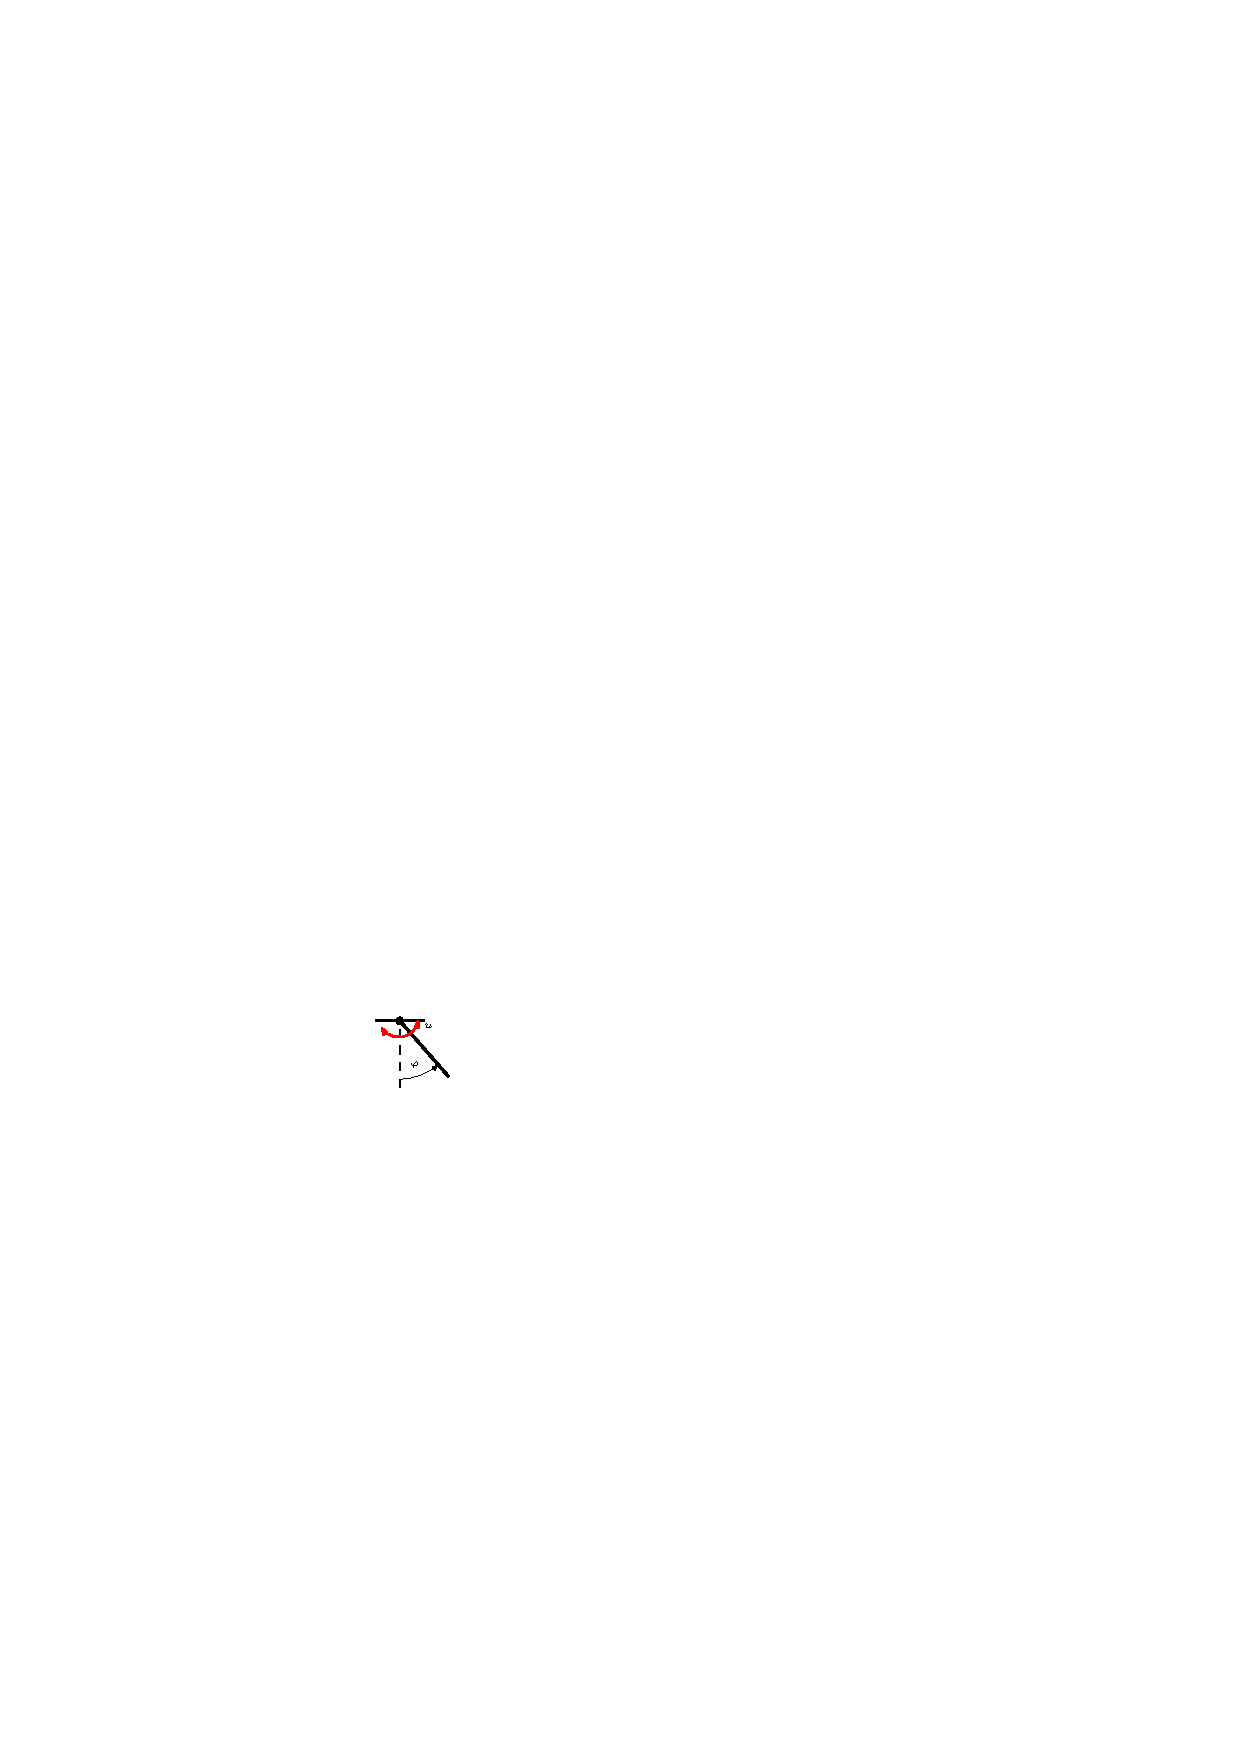
\includegraphics[height= 2cm]{./figures/pendulum}
\caption{Pendulum.}\label{fig:pendulum}
\end{figure}

The pendulum shown in Figure~\ref{fig:pendulum} possesses a mass $m$
and a length $l$. The pendulum angle $\varphi$ is measured
anti-clockwise from hanging down. A torque $u$ can be applied to the
pendulum. Typical values are: $m=\unit[1]{kg}$ and $l=\unit[1]{m}$.

The coordinates $x$ and $y$ of the midpoint of the pendulum are
\begin{align*}
x&=\tfrac{1}{2}l\sin\varphi\,,\\
y&=-\tfrac{1}{2}l\cos\varphi,
\end{align*}
and the squared velocity of the  midpoint of the pendulum is
\begin{align*}
v^2&=\dot x^2+\dot y^2 = \tfrac{1}{4}l^2\dot\varphi^2\,.
\end{align*}
We derive the equations of motion via the system Lagrangian $L$, which
is the difference between kinetic energy $T$ and potential energy $V$
and given by
\begin{equation}\label{eq:Lagrangian1 pend}
L=T-V=
\tfrac{1}{2}mv^2+\tfrac{1}{2}I\dot\varphi^2+\tfrac{1}{2}mlg\cos\varphi\,,
\end{equation}
where $g=\unit[9.82]{m/s^2}$ is the acceleration of gravity and
$I=\tfrac{1}{12}ml^2$ is the moment of inertia of a pendulum
around the pendulum midpoint. 

The equations of motion can generally be derived from a set of equations
defined through
\begin{equation*}
\frac{d}{d t}\frac{\partial L}{\partial\dot q_i}-\frac{\partial
  L}{\partial q_i}=Q_i\,,
\end{equation*}
where $Q_i$ are the non-conservative forces and $q_i$ and $\dot q_i$
are the state variables of the system. In our case,
\begin{align*}
  \frac{\partial
    L}{\partial\dot\varphi}&=\tfrac{1}{4}ml^2\dot\varphi+I\dot\varphi\\
  \frac{\partial L}{\partial\varphi}&=-\tfrac{1}{2}mlg\sin\varphi
\end{align*}
yield
\begin{align*}
\ddot\varphi(\tfrac{1}{4}ml^2+I)+\tfrac{1}{2}mlg\sin\varphi=u-b\dot\varphi\,,
\end{align*}
where $b$ is a friction coefficient. Collecting both variables $\vec
z=[\dot\varphi,\varphi]\T$ the equations of motion can be conveniently
expressed as two coupled ordinary differential equations
\begin{align*}
\frac{d\vec z}{d t}=
\begin{bmatrix}
\displaystyle
\frac{u-bz_1-\tfrac{1}{2}mlg\sin z_2}{\tfrac{1}{4}ml^2+I}\\
z_1
\end{bmatrix}\,,
\end{align*}
which can be simulated numerically.

\section{Double Pendulum Swing-up with a Single Actuator (Pendubot)}  
\label{sec:pendubot}
\begin{figure}[tb]
\centering
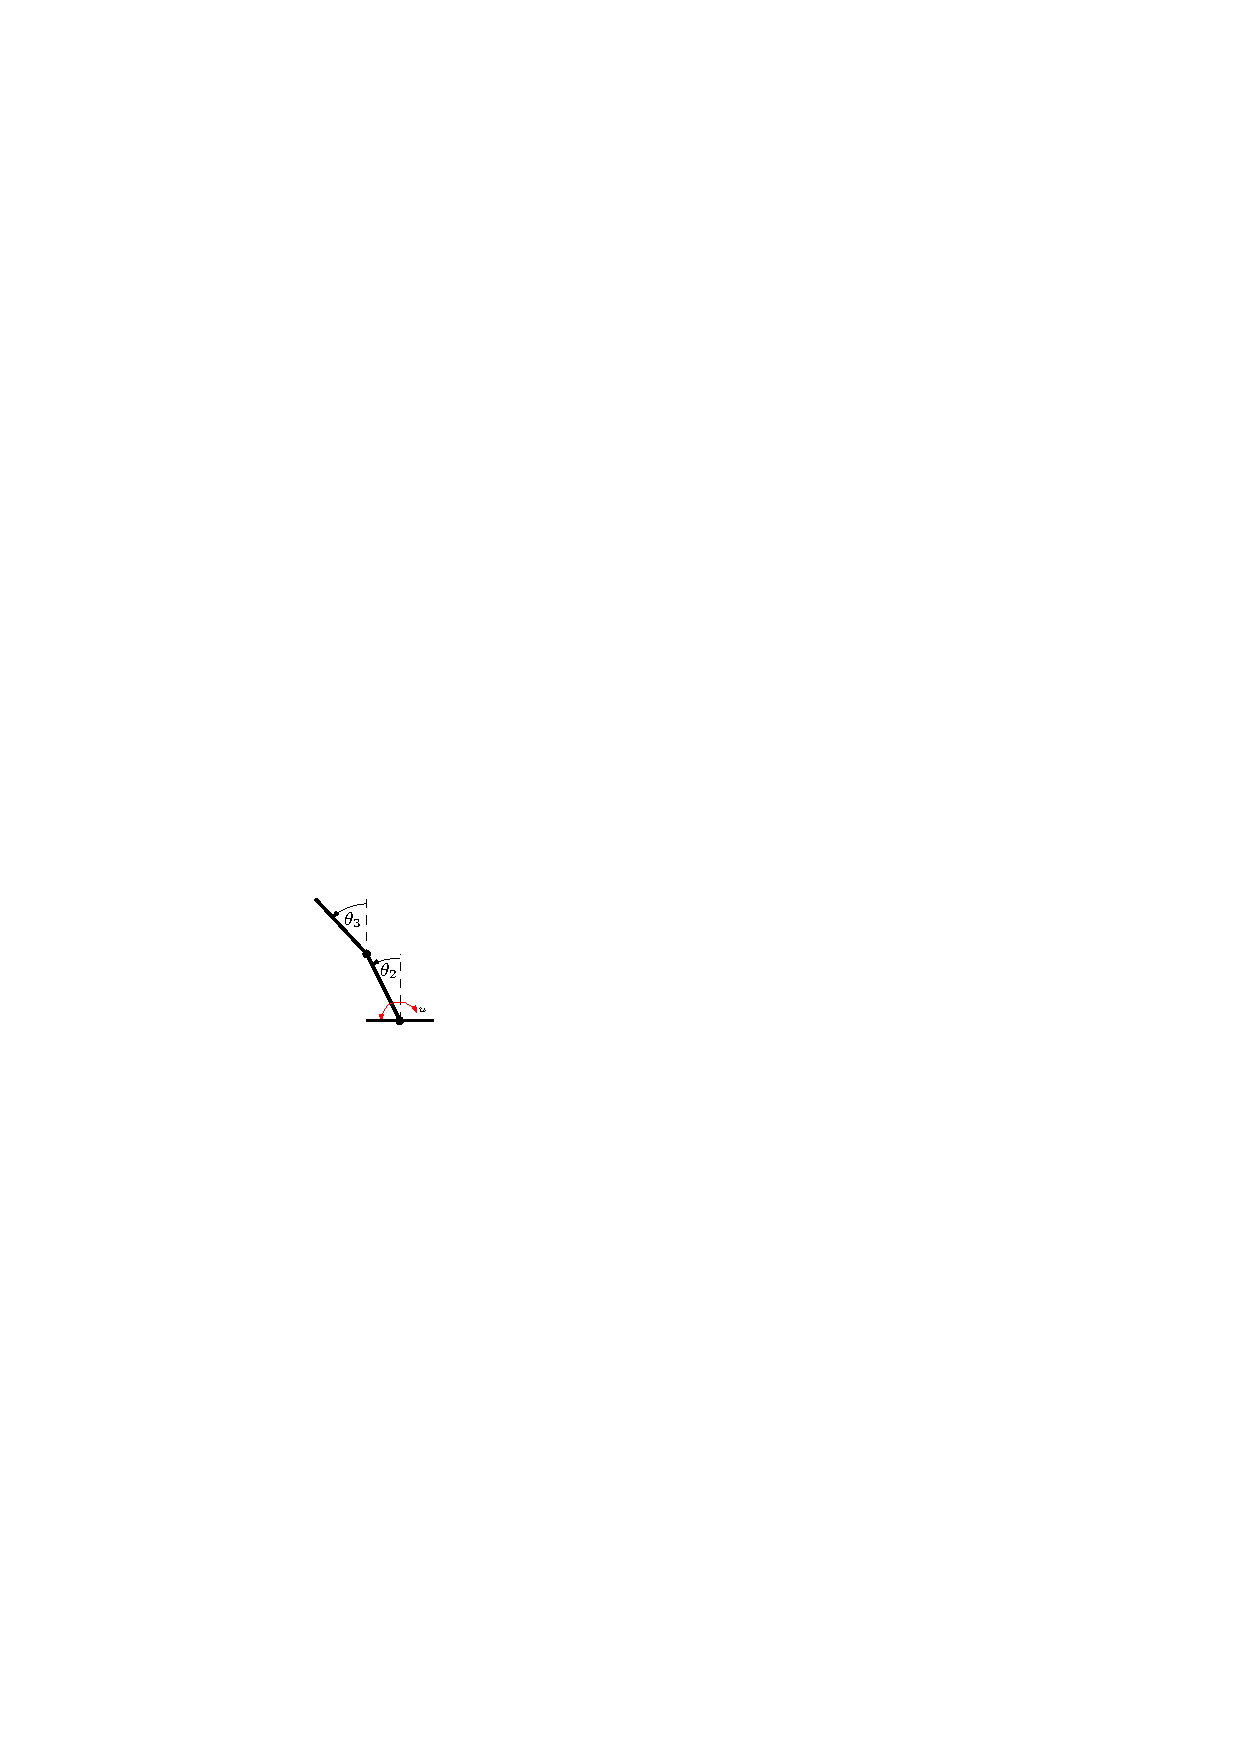
\includegraphics[height=3.5cm]{./figures/pendubot}
\caption{Pendubot.}\label{fig:pendubot}
\end{figure}


The Pendubot in Figure~\ref{fig:pendubot} is a two-link (mass $m_2$
and $m_3$ and length s $l_2$ and $l_3$ respectively), underactuated
robot as described by~\cite{Spong1995}. The first joint exerts torque,
but the second joint cannot. The system has four continuous state
variables: two joint positions and two joint velocities. The angles of
the joints, $\theta_2$ and $\theta_3$, are measured anti-clockwise
from upright. An applied external torque $u$ controls the first
joint. Typical values are: $m_2=0.5{\rm kg}$, $m_3=0.5{\rm kg}$
$l_2=0.6{\rm m}$, $l_3=0.6{\rm m}$.

The Cartesian coordinates $x_2$, $y_2$ and $x_3$, $y_3$ of the midpoints of the
pendulum elements are
\begin{equation}
\begin{bmatrix}
x_2\\y_2
\end{bmatrix}
=
\begin{bmatrix}
-\tfrac{1}{2}l_2\sin\theta_2\\
\tfrac{1}{2}l_2\cos\theta_2 
\end{bmatrix}\,,\quad
\begin{bmatrix}
x_3\\y_3
\end{bmatrix}
=
\begin{bmatrix}
-l_2\sin\theta_2-\tfrac{1}{2}l_3\sin\theta_3\\
l_2\cos\theta_2+\tfrac{1}{2}l_3\cos\theta_3
\end{bmatrix}\,,
\end{equation}
and the squared velocities of the pendulum midpoints are
\begin{align}
v_2^2&=\dot x_2^2+\dot
y_2^2=\tfrac{1}{4}l_2^2\dot\theta_2^2\label{eq:pendubot v2}\\
v_3^2&=\dot x_3^2+\dot y_3^2=l_2^2\dot\theta_2^2+
\tfrac{1}{4}l_3^2\dot\theta_3^2+
l_2l_3\dot\theta_2\dot\theta_3\cos(\theta_2-\theta_3)\label{eq:pendubot
v3}.
\end{align}
The system Lagrangian is the difference between the kinematic energy $T$ and
the potential energy $V$ and given by
\begin{align*}
L&=T-V=\tfrac{1}{2}m_2v_2^2+\tfrac{1}{2}m_3v_3^2+
\tfrac{1}{2}I_2\dot\theta_2^2+\tfrac{1}{2}I_3\dot\theta_3^2-m_2gy_2-m_3gy_3\,,
\end{align*}
where the angular moment of inertia around the pendulum midpoint is
$I=\tfrac{1}{12}ml^2$, and $g=9.82 {\rm m/s^2}$ is the acceleration of
gravity. Using this moment of inertia, we assume that the pendulum is
a thin (but rigid) wire.  Plugging in the squared
velocities~(\ref{eq:pendubot v2}) and~\eqref{eq:pendubot v3}, we
obtain
\begin{align*}
L&=\tfrac{1}{8}m_2l_2^2\dot\theta_2^2+\tfrac{1}{2}m_3\big(l_2^2\dot\theta_2^2 +
\tfrac{1}{4}
l_3^2\dot\theta_3^2+l_2l_3\dot\theta_2\dot\theta_3\cos(\theta_2-\theta_3)\big)\\
&\quad + \tfrac{1}{2}I_2\dot\theta_2^2+\tfrac{1}{2}I_3\dot\theta_3^2
-\tfrac{1}{2}m_2gl_2\cos\theta_2-m_3g(l_2\cos\theta_2 +
\tfrac{1}{2}l_3\cos\theta_3)\,.
\end{align*}
%
The equations of motion are
\begin{equation}
\frac{d}{d t}\frac{\partial L}{\partial\dot q_i}-\frac{\partial
  L}{\partial q_i}=Q_i\,,
\end{equation}
where $Q_i$ are the non-conservative forces and $q_i$ and $\dot q_i$ are the
state variables of the system. In our case,
\begin{align*}
\frac{\partial L}{\partial\dot\theta_2} &=
l_2^2\dot\theta_2(\tfrac{1}{4}m_2+m_3) +
\tfrac{1}{2}m_3l_2l_3\dot\theta_3\cos(\theta_2-\theta_3) + I_2\dot\theta_2\,,\\
\frac{\partial L}{\partial\theta_2} & =
-\tfrac{1}{2}m_3l_2l_3\dot\theta_2\dot\theta_3\sin(\theta_2-\theta_3) +
(\tfrac{1}{2}m_2+m_3)gl_2\sin\theta_2\,,\\
\frac{\partial L}{\partial\dot\theta_3}&= m_3l_3\big(\tfrac{1}{4}
l_3\dot\theta_3 +
\tfrac{1}{2} l_2\dot\theta_2\cos(\theta_2-\theta_3)\big) + I_3\dot\theta_3\,,\\
\frac{\partial L}{\partial\theta_3}&=
\tfrac{1}{2}m_3l_3\big(l_2\dot\theta_2\dot\theta_3\sin(\theta_2-\theta_3) +
g\sin\theta_3\big)
\end{align*}
lead to the equations of motion
\begin{align*}
u &= \ddot\theta_{2}\big(l_2^2(\tfrac{1}{4}m_2+m_3) + I_2\big) +
\ddot\theta_3\tfrac{1}{2}m_3l_3l_2\cos(\theta_2-\theta_3)\nonumber \\
&\quad+
l_2\big(\tfrac{1}{2}
m_3l_3\dot\theta_3^2\sin(\theta_2-\theta_3)-g\sin\theta_2(\tfrac{1}{2}
m_2+m_3)\big)\,,\\
0&=\ddot\theta_2\tfrac{1}{2}l_2l_3m_3\cos(\theta_2-\theta_3)+\ddot\theta_3(\tfrac{1
}{
4}m_3l_3^2+I_3)-\tfrac{1}{2}m_3l_3\big(
l_2\dot\theta_2^2\sin(\theta_2-\theta_3)+g\sin\theta_3\big)\,.
\end{align*}
To simulate the system numerically, we solve the linear equation system
\begin{align*}
\begin{bmatrix}
l_2^2(\tfrac{1}{4}m_2+m_3) + I_2 &
\tfrac{1}{2}m_3l_3l_2\cos(\theta_2-\theta_3)\\
\tfrac{1}{2}l_2l_3m_3\cos(\theta_2-\theta_3) & \tfrac{1}{
4}m_3l_3^2+I_3
\end{bmatrix}
\begin{bmatrix}
\ddot\theta_2\\
\ddot\theta_3
\end{bmatrix}
=
\begin{bmatrix}
c_2\\
c_3
\end{bmatrix}
\end{align*}
for $\ddot\theta_2$ and $\ddot\theta_3$, where
\begin{align*}
\begin{bmatrix}
c_2\\c_3
\end{bmatrix}
=
\begin{bmatrix}
-l_2\big(\tfrac{1}{2}
m_3l_3\dot\theta_3^2\sin(\theta_2-\theta_3)-g\sin\theta_2(\tfrac{1}{2}
m_2+m_3)\big) + u\\
\tfrac{1}{2}m_3l_3\big(
l_2\dot\theta_2^2\sin(\theta_2-\theta_3)+g\sin\theta_3\big)
\end{bmatrix}\,.
\end{align*}


\section{Double Pendulum Swing-up with Two Actuators}
The dynamics of the double pendulum with two actuators (one at the
shoulder, one at the elbow), are derived exactly as described in
Section~\ref{sec:pendubot}, with the single modification that we need
to take the second control signal into account in the equations of
motion
\begin{align*}
u_1 &= \ddot\theta_{2}\big(l_2^2(\tfrac{1}{4}m_2+m_3) + I_2\big) +
\ddot\theta_3\tfrac{1}{2}m_3l_3l_2\cos(\theta_2-\theta_3)\nonumber \\
&\quad+
l_2\big(\tfrac{1}{2}
m_3l_3\dot\theta_3^2\sin(\theta_2-\theta_3)-g\sin\theta_2(\tfrac{1}{2}
m_2+m_3)\big)\,,\\
u_2&=\ddot\theta_2\tfrac{1}{2}l_2l_3m_3\cos(\theta_2-\theta_3)+\ddot\theta_3(\tfrac{1
}{
4}m_3l_3^2+I_3)-\tfrac{1}{2}m_3l_3\big(
l_2\dot\theta_2^2\sin(\theta_2-\theta_3)+g\sin\theta_3\big)\,.
\end{align*}
To simulate the system numerically, we solve the linear equation system
\begin{align*}
\begin{bmatrix}
l_2^2(\tfrac{1}{4}m_2+m_3) + I_2 &
\tfrac{1}{2}m_3l_3l_2\cos(\theta_2-\theta_3)\\
\tfrac{1}{2}l_2l_3m_3\cos(\theta_2-\theta_3) & \tfrac{1}{
4}m_3l_3^2+I_3
\end{bmatrix}
\begin{bmatrix}
\ddot\theta_2\\
\ddot\theta_3
\end{bmatrix}
=
\begin{bmatrix}
c_2\\
c_3
\end{bmatrix}
\end{align*}
for $\ddot\theta_2$ and $\ddot\theta_3$, where
\begin{align*}
\begin{bmatrix}
c_2\\c_3
\end{bmatrix}
=
\begin{bmatrix}
-l_2\big(\tfrac{1}{2}
m_3l_3\dot\theta_3^2\sin(\theta_2-\theta_3)-g\sin\theta_2(\tfrac{1}{2}
m_2+m_3)\big) + u_1\\
\tfrac{1}{2}m_3l_3\big(
l_2\dot\theta_2^2\sin(\theta_2-\theta_3)+g\sin\theta_3\big)+u_2
\end{bmatrix}\,.
\end{align*}



\section{Cart-Pole Swing-up}
\begin{wrapfigure}{r}{0.4\hsize}
\vspace{-5mm}
\centering
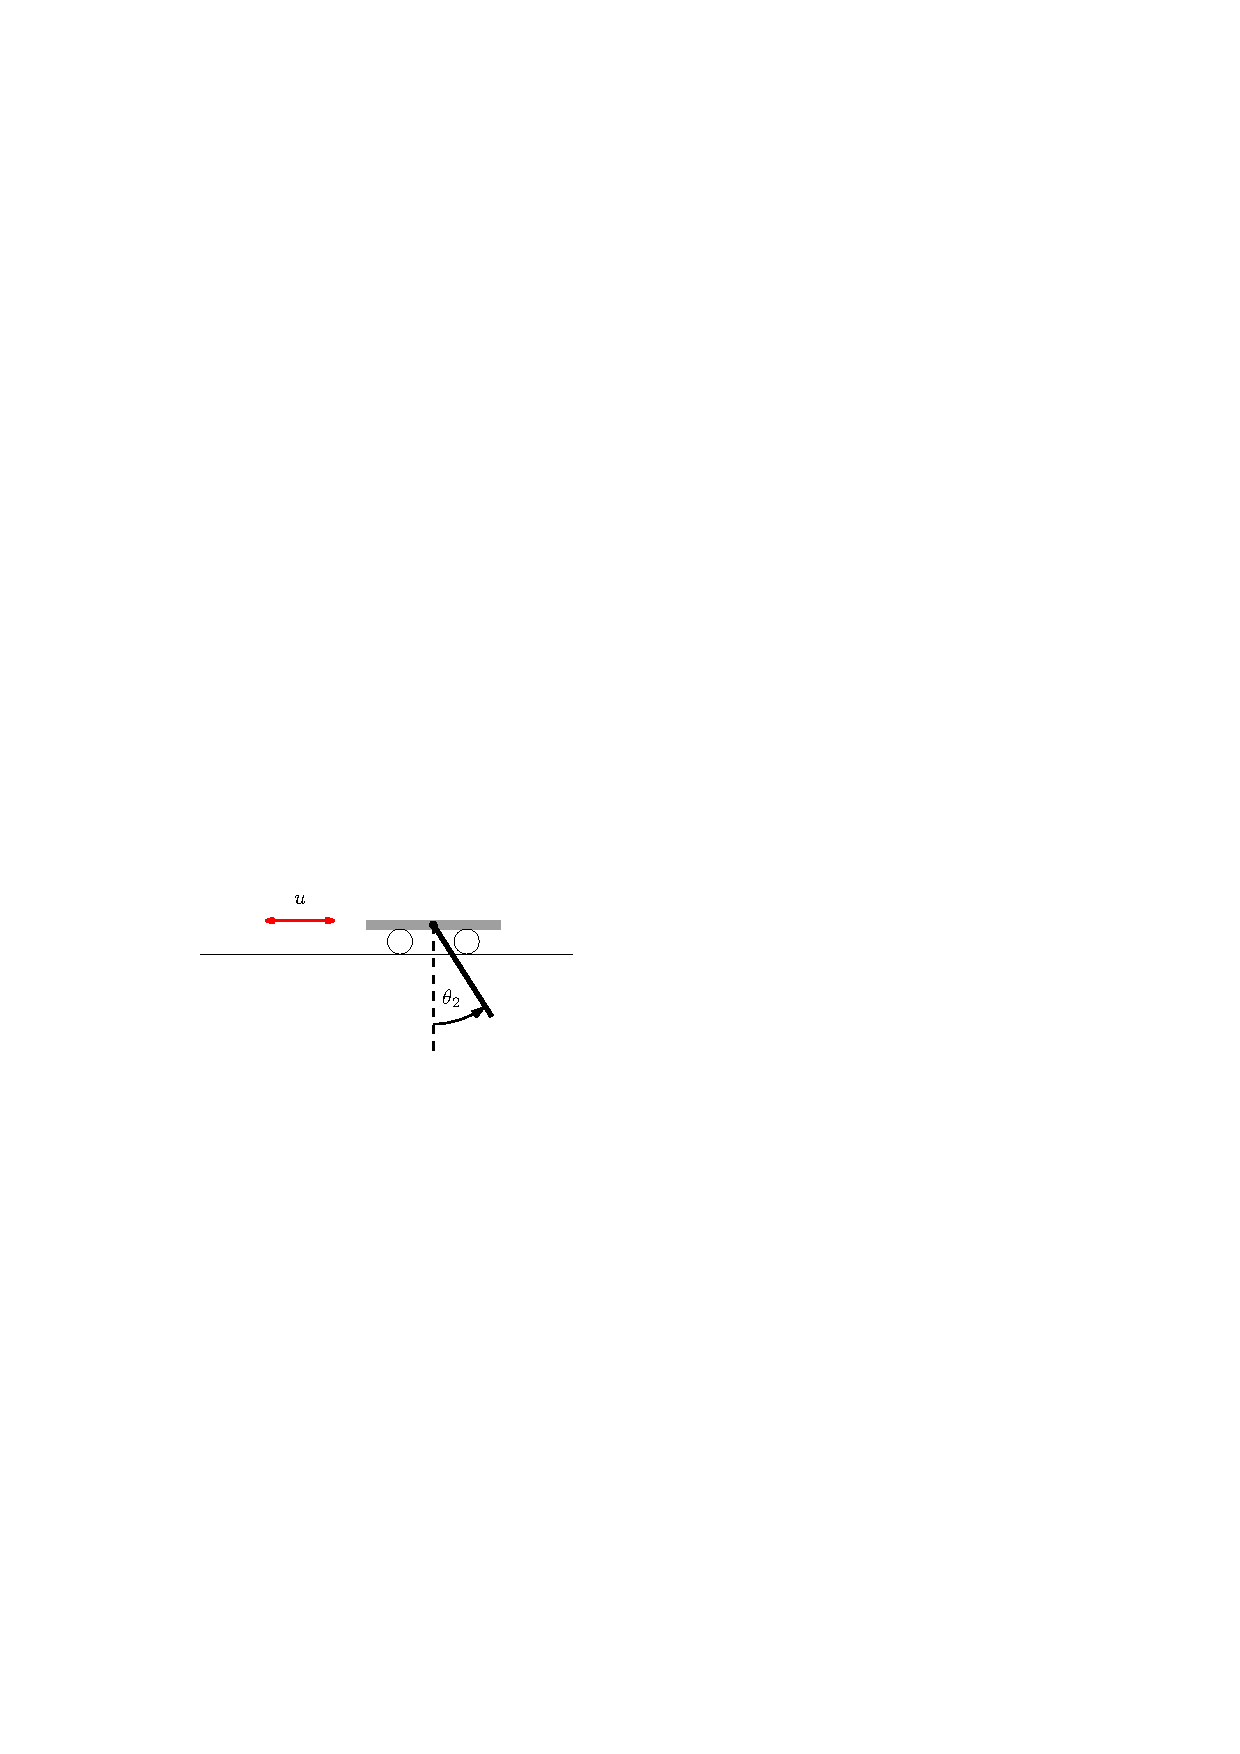
\includegraphics[width=\hsize]{./figures/cp}
\caption{Cart-pole system.}\label{fig:cp}
\end{wrapfigure}
%
The cart-pole system (inverted pendulum) shown in Figure~\ref{fig:cp}
consists of a cart with mass $m_1$ and an attached pedulum with mass
$m_2$ and length $l$, which swings freely in the plane. The pendulum
angle $\theta_2$ is measured anti-clockwise from hanging down. The
cart can move horizontally with an applied external force $u$ and a
parameter $b$, which describes the friction between cart and
ground. Typical values are: $m_1=\unit[0.5]{kg}$,
$m_2=\unit[0.5]{kg}$, $l=\unit[0.6]{m}$ and $b=\unit[0.1]{N/m/s}$.

The position of the cart along the track is denoted by $x_1$. The
coordinates $x_2$ and $y_2$ of the midpoint of the pendulum are
\begin{align*}
x_2&=x_1+\tfrac{1}{2}l\sin\theta_2\,,\\
y_2&=-\tfrac{1}{2}l\cos\theta_2,
\end{align*}
and the squared velocity of the cart and the midpoint of the pendulum are
\begin{align*}
v_1^2&=\dot x_1^2\\
v_2^2&=\dot x_2^2+\dot y_2^2 = \dot
x_1^2+\tfrac{1}{4}l^2\dot\theta_2^2+l\dot x_1\dot\theta_2\cos\theta_2\,,
\end{align*}
respectively. We derive the equations of motion via the system
Lagrangian $L$, which is the difference between kinetic energy $T$ and
potential energy $V$ and given by
\begin{equation}\label{eq:Lagrangian1 cp}
L=T-V=
\tfrac{1}{2}m_1v_1^2+\tfrac{1}{2}m_2v_2^2+\tfrac{1}{2}I\dot\theta_2^2-m_2gy_2\,,
\end{equation}
where $g=\unit[9.82]{m/s^2}$ is the acceleration of gravity and
$I=\tfrac{1}{12}ml^2$ is the moment of inertia of a pendulum around the
pendulum midpoint. Pluggin
this value for $I$ into the system Lagrangian~(\ref{eq:Lagrangian1 cp}), we
obtain
\begin{align*}
L=\tfrac{1}{2}(m_1+m_2)\dot
x_1^2+\tfrac{1}{6}m_2l^2\dot\theta_2^2+\tfrac{1}{2}m_2l(\dot
x_1\dot\theta_2+g)\cos\theta_2\,.
\end{align*}

The equations of motion can generally be derived from a set of equations
defined through
\begin{equation}
\frac{d}{d t}\frac{\partial L}{\partial\dot q_i}-\frac{\partial
  L}{\partial q_i}=Q_i\,,
\end{equation}
where $Q_i$ are the non-conservative forces and $q_i$ and $\dot q_i$ are the
state variables of the system. In our case,
\begin{align*}
\frac{\partial L}{\partial\dot x_1}&=
(m_1+m_2)\dot x_1+\tfrac{1}{2}m_2l\dot\theta_2\cos\theta_2\,,\\
\frac{\partial L}{\partial x_1}&=0\,,\\
\frac{\partial
  L}{\partial\dot\theta_2}&=\tfrac{1}{3}m_2l^2\dot\theta_2
+\tfrac{1}{2}m_2l\dot x_1\cos\theta_2\,,\\
\frac{\partial L}{\partial\theta_2}&=-\tfrac{1}{2}m_2l(\dot
x_1\dot\theta_2+g),
\end{align*}
lead to the equations of motion
\begin{align*}
(m_1+m_2)\ddot x_1+\tfrac{1}{2}m_2l\ddot\theta_2\cos\theta_2
-\tfrac{1}2m_2l\dot\theta_2^2\sin\theta_2&=u-b\dot x_1\,,\\
2l\ddot\theta_2+3\ddot x_1\cos\theta_2+3g\sin\theta_2&=0\,.
\end{align*}
Collecting the four variables $\vec z=[x_1,\dot x_1,\dot\theta_2,\theta_2]\T$
the equations of motion can be conveniently expressed as four coupled
ordinary differential equations
\begin{align*}
\frac{d\vec z}{d t}=
\begin{bmatrix}
z_2\\[2mm]
\displaystyle
\frac{2m_2l z_3^2\sin z_4+3m_2g\sin z_4\cos z_4+4u-4bz_2}
{4(m_1+m_2)-3m_2\cos^2 z_4}\\[2mm]
\displaystyle
\frac{-3m_2l z_3^2\sin z_4\cos z_4-6(m_1+m_2)g\sin z_4-6(u-bz_2)\cos z_4}
{4l(m_1+m_2)-3m_2l\cos^2 z_4} \\
z_3
\end{bmatrix}\,,
\end{align*}
which can be simulated numerically.




\section{Cart-Double Pendulum Swing-up}
\begin{wrapfigure}{r}{0.3\hsize}
\vspace{-5mm}
\centering
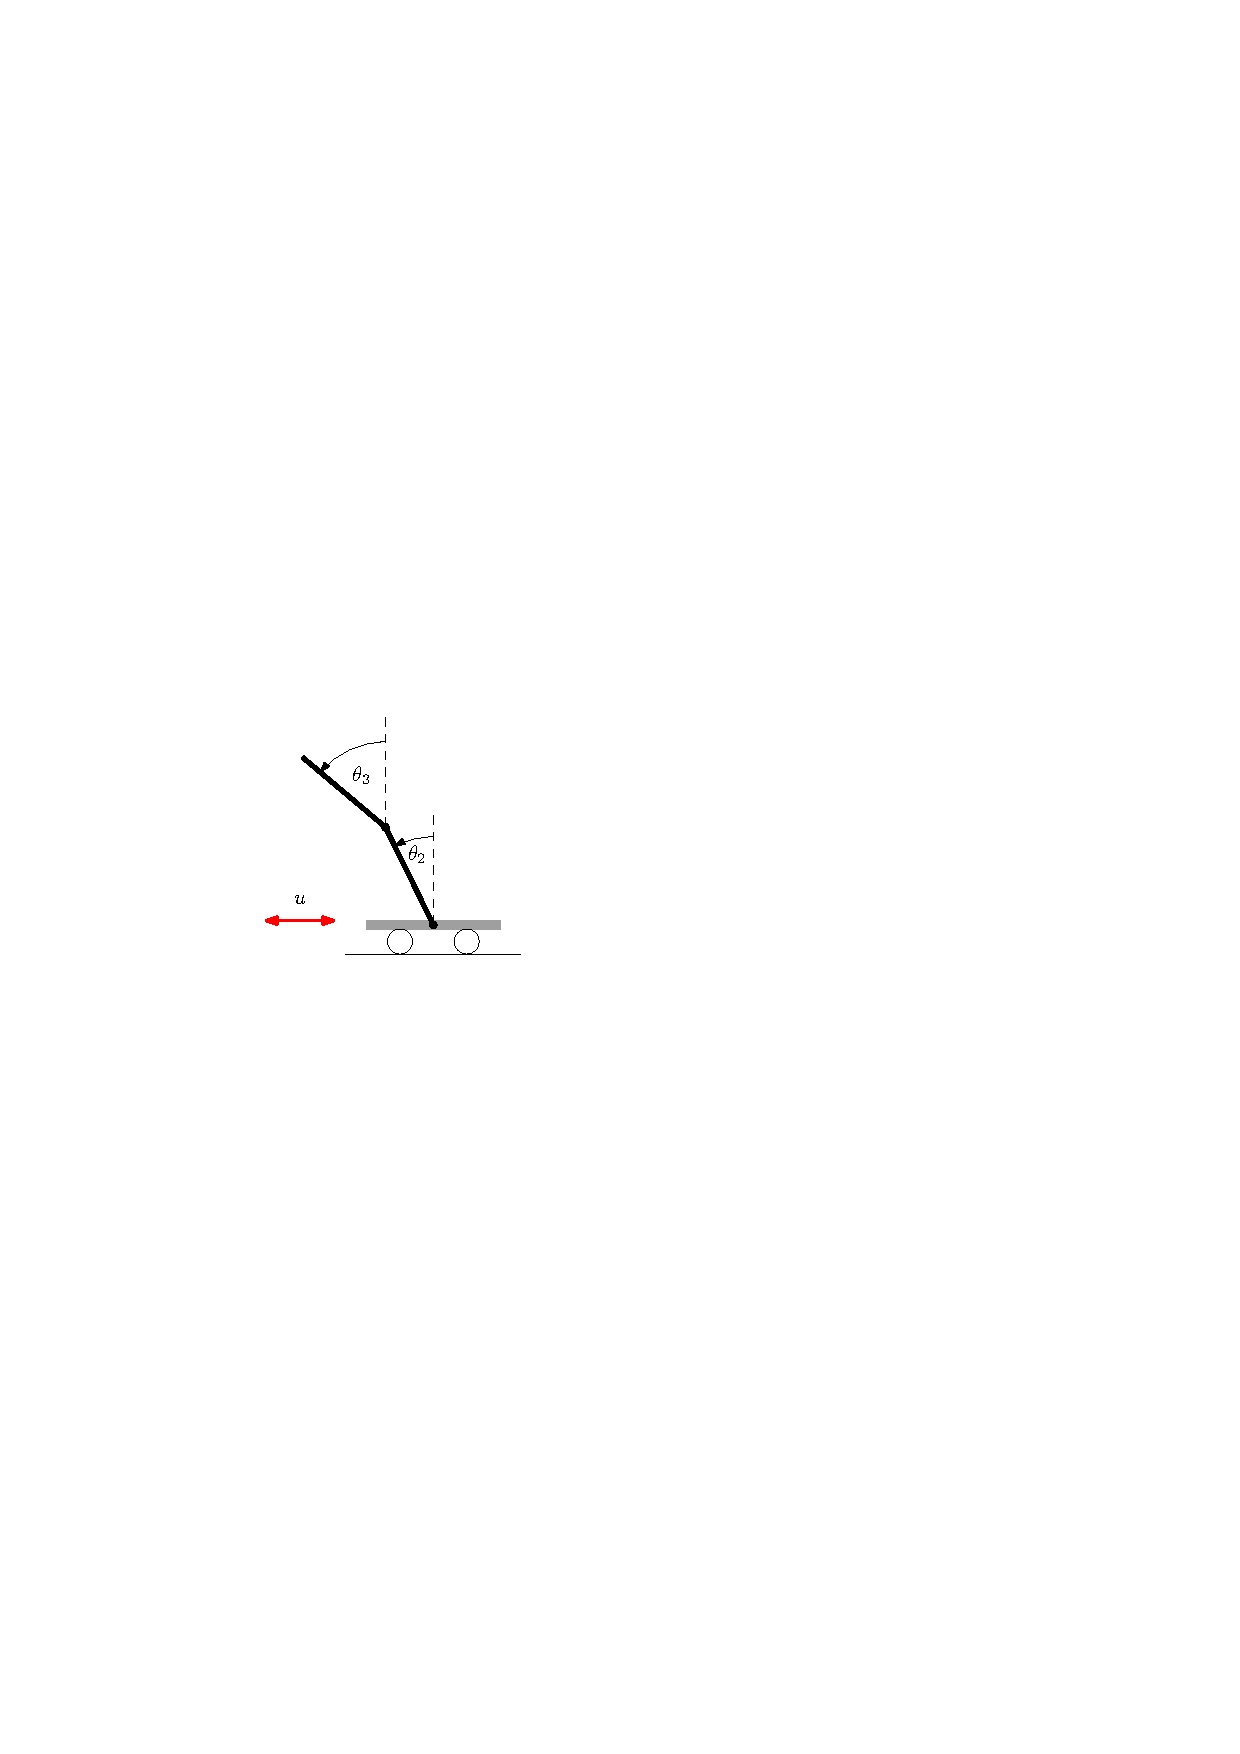
\includegraphics[width = \hsize]{./figures/cdp_sketch}
\caption{Cart-double pendulum.}
\label{fig:cdp dyn}
\end{wrapfigure}
%
The cart-double pendulum dynamic system (see Figure~\ref{fig:cdp dyn})
consists of a cart with mass $m_1$ and an attached double pendulum
with masses $m_2$ and $m_3$ and lengths $l_2$ and $l_3$ for the two
links, respectively. The double pendulum swings freely in the
plane. The angles of the pendulum, $\theta_2$ and $\theta_3$, are
measured anti-clockwise from upright. The cart can move horizontally,
with an applied external force $u$ and the coefficient of friction
$b$. Typical values are: $m_1=\unit[0.5]{kg}$, $m_2=\unit[0.5]{kg}$,
$m_3=\unit[0.5]{kg}$ $l_2=\unit[0.6]{m}$, $l_3=\unit[0.6]{m}$, and
$b=\unit[0.1]{Ns/m}$.

The coordinates, $x_2$, $y_2$ and $x_3$, $y_3$ of the midpoint of the
pendulum elements are
\begin{align*}
\begin{bmatrix}
x_2\\
y_2
\end{bmatrix}
&=
\begin{bmatrix}
x_1-\tfrac{1}{2}l_2\sin\theta_2\\
\tfrac{1}{2}l_2\cos\theta_2
\end{bmatrix}\\
\begin{bmatrix}
x_3\\
y_3
\end{bmatrix}
&=
\begin{bmatrix}
x_1-l_2\sin\theta_2-\tfrac{1}{2}l_3\sin\theta_3\\
y_3=l_2\cos\theta_2+\tfrac{1}{2}l_3\cos\theta_3
\end{bmatrix} \,.
\end{align*}
The squared velocities of the cart and the pendulum midpoints are
\begin{align*}
v_1^2&=\dot x_1^2\,,\\
v_2^2&=\dot x_2^2+\dot y_2^2=\dot x_1^2-
l_2\dot x_1\dot\theta_2\cos\theta_2+\tfrac{1}{4}l_2^2\dot\theta_2^2\,,\\
v_3^2&=\dot x_3^2+\dot y_3^2=\dot x_1^2+l_2^2\dot\theta_2^2+
\tfrac{1}{4}l_3^2\dot\theta_3^2-2l_2\dot x_1\dot\theta_2\cos\theta_2-
l_3\dot x_1\dot\theta_3\cos\theta_3+
l_2l_3\dot\theta_2\dot\theta_3\cos(\theta_2-\theta_3)\,.
\end{align*}
The system Lagrangian is the difference between the kinematic energy
$T$ and the potential energy $V$ and given by
\begin{align*}
  L&=T-V=\tfrac{1}{2}m_1v_1^2+\tfrac{1}{2}m_2v_2^2+\tfrac{1}{2}m_3v_3^2+
  \tfrac{1}{2}I_2\dot\theta_2^2+\tfrac{1}{2}I_3\dot\theta_3^2-m_2gy_2-m_3gy_3
  \\
  &= \tfrac{1}{2}(m_1+m_2+m_3)\dot x_1^2 -\tfrac{1}{2} m_2l_2\dot
  x\dot\theta_2\cos(\theta_2) - \tfrac{1}{2}m_3\big(2l_2\dot
  x\dot\theta_2\cos(\theta_2) + l_3\dot
  x_1\dot\theta_3\cos(\theta_3)\big)\nonumber \\
  &\quad + \tfrac{1}{8} m_2l_2^2\dot\theta_2^2+
  \tfrac{1}{2}I_2\dot\theta_2^2 + \tfrac{1}{2}m_3(l_2^2\dot\theta_2^2
  + \tfrac{1}{4}l_3^2\dot\theta_3^2 +
  l_2l_3\dot\theta_2\dot\theta_3\cos(\theta_2-\theta_3)) +
  \tfrac{1}{2}I_3\dot\theta_3^2\nonumber  \\
  &\quad - \tfrac{1}{2}m_2gl_2\cos(\theta_2) -
  m_3g(l_2\cos(\theta_2)+\tfrac{1}{2}l_3\cos(\theta_3))\,.
% &=\tfrac{1}{2}(m_1+m_2+m_3)\dot x_1^2+
% (\tfrac{1}{6}m_2+\tfrac{1}{2}m_3)l_2^2\dot\theta_2^2+
% \tfrac{1}{6}m_3l_3^2\dot\theta_3^2-
% (\tfrac{1}{2}m_2+m_3)l_2\dot x_1\dot\theta_2\cos\theta_2\\
% &\quad-\tfrac{1}{2}m_3l_3\dot x_1\dot\theta_3\cos\theta_3+
% \tfrac{1}{2}m_3l_2l_3\dot\theta_2\dot\theta_3\cos(\theta_2-\theta_3)-
% (\tfrac{1}{2}m_2+m_3)l_2g\cos\theta_2-\tfrac{1}{2}m_3l_3g\cos\theta_3,
\end{align*}
The angular moment of inertia $I_j$, $j=2,3$ around the pendulum
midpoint is $I_j=\tfrac{1}{12}ml_j^2$, and $g=\unit[9.82]{m/s^2}$ is
the acceleration of gravity. These moments inertia imply the
assumption that the pendulums are thin (but rigid) wires.

The equations of motion are
\begin{equation}
\frac{d}{d t}\frac{\partial L}{\partial\dot q_i}-\frac{\partial
  L}{\partial q_i}=Q_i\,,
\end{equation}
where $Q_i$ are the non-conservative forces. 
We obtain the partial derivatives
\begin{align*}
  \frac{\partial L}{\partial \dot x_1}&= (m_1+m_2+m_3)\dot
  x_1-(\tfrac{1}{2}m_2+m_3)l_2\dot\theta_2
  \cos\theta_2-\tfrac{1}{2}m_3l_3\dot\theta_3\cos\theta_3\,,\\
  \frac{\partial L}{\partial x_1}&=0\,,\\
  \frac{\partial L}{\partial\dot\theta_2}&=
  (m_3l_2^2+\tfrac{1}{4}m_2l_2^2+I_2)\dot\theta_2 -
  (\tfrac{1}{2}m_2+m_3)l_2\dot x_1\cos\theta_2+
  \tfrac{1}{2}m_3l_2l_3\dot\theta_3\cos(\theta_2-\theta_3)\,,\\
  \frac{\partial L}{\partial\theta_2}&=
  (\tfrac{1}{2}m_2+m_3)l_2(\dot
  x_1\dot\theta_2+g)\sin\theta_2-\tfrac{1}{2}
  m_3l_2l_3\dot\theta_2\dot\theta_3\sin(\theta_2-\theta_3)\,,\\
  \frac{\partial L}{\partial\dot\theta_3}&=
  m_3l_3\big[-\tfrac{1}{2}\dot x_1\cos\theta_3+
  \tfrac{1}{2}l_2\dot\theta_2\cos(\theta_2-\theta_3)+\tfrac{1}{4}l_3\dot\theta_3\big]+I_3\dot\theta_3\,,\\
  \frac{\partial L}{\partial\theta_3}&= \tfrac{1}{2}m_3l_3\big[(\dot
  x_1\dot\theta_3+g)\sin\theta_3+
  l_2\dot\theta_2\dot\theta_3\sin(\theta_2-\theta_3)\big]
\end{align*}
leading to the equations of motion
\begin{align*}
  (m_1+m_2+m_3)\ddot x_1+\tfrac{1}{2}m_2+m_3)l_2
  (\dot\theta_2^2\sin\theta_2-\ddot\theta_2\cos\theta_2)\nonumber\\
  \quad +
  \tfrac{1}{2}m_3l_3(\dot\theta_3^2\sin\theta_3-\ddot\theta_3\cos\theta_3)
  &=u-b\dot x_1\\
  (m_3l_2^2+I_2+\tfrac{1}{4}m_2l_2^2)\ddot\theta_2
  -(\tfrac{1}{2}m_2+m_3)l_2(\ddot
  x_1\cos\theta_2+g\sin\theta_2)\nonumber\\
  \quad+ \tfrac{1}{2}m_3l_2l_3[\ddot\theta_3\cos(\theta_2-\theta_3)
  +\dot\theta_3^2\sin(\theta_2-\theta_3)]&=0\\
% 2l_3\ddot\theta_3+3l_2[\ddot\theta_2\cos(\theta_2-\theta_3)-
% \dot\theta_2^2\sin(\theta_2-\theta_3)]-
% 3\ddot x_1\cos\theta_3-3g\sin\theta_3&=0\\
(\tfrac{1}{4}m_2 l_3^2+I_3)\ddot\theta_3 -\tfrac{1}{2}m_3l_3(\ddot
x_1\cos\theta_3 + g\sin\theta_3)\nonumber \\
\quad + \tfrac{1}{2}m_3l_2l_3[\ddot\theta_2\cos(\theta_2-\theta_3)-\dot\theta_2^2\sin(\theta_2-\theta_3)] & = 0
\end{align*}
%solve([(m1+m2+m3)*ddx-(m2/2+m3)*l2*cos(t2)*ddt2-m3*l3*cos(t3)/2*ddt3=u-b*dx1-(m2/2+m3)*l2*dt2*dt2*sin(t2)-m3*l3*dt3*dt3*sin(t3)/2,-(m2/2+m3)*cos(t2)*ddx+(m2/3+m3)*l2*ddt2+m3*l3*cos(t2-t3)/2=(m2/2+m3)*g*sin(t2)-m3*l3*dt3*dt3*sin(t2-t3)/2,-3*cos(t3)*ddx+3*l2*cos(t2-t3)*ddt2+2*l3*ddt3=3*l2*dt2*dt2*sin(t2-t3)+3*(dx1*dt3+g)*sin(t3)],[ddx,ddt2,ddt3]);
These three linear equations in $(\ddot x_1, \ddot\theta_2,
\ddot\theta_3)$ can be rewritten as the linear equation system
\begin{align*}
\begin{bmatrix}
(m_1+m_2+m_3) &
-\tfrac{1}{2}(m_2+2m_3)l_2\cos\theta_2 &
-\tfrac{1}{2}m_3l_3\cos\theta_3\\
-(\tfrac{1}{2}m_2+m_3)l_2\cos\theta_2
& m_3l_2^2+I_2+\tfrac{1}{4}m_2l_2^2
& \tfrac{1}{2}m_3l_2l_3\cos(\theta_2-\theta_3)
\\
-\tfrac{1}{2}m_3l_3\cos\theta_3
& 
\tfrac{1}{2}m_3l_2l_3\cos(\theta_2-\theta_3)
& \tfrac{1}{4}m_2l_3^2+I_3
\end{bmatrix}
\begin{bmatrix}
\ddot x_1 \\
\ddot\theta_2 \\ \ddot\theta_3
\end{bmatrix}
 =
\begin{bmatrix}
c_1\\c_2\\c_3
\end{bmatrix}\,,
\end{align*}
where
\begin{align*}
&
\begin{bmatrix}
c_1\\c_2\\c_3
\end{bmatrix}
=
\begin{bmatrix}
u-b\dot x_1-\tfrac{1}{2}(m_2+2m_3)l_2
\dot\theta_2^2\sin\theta_2-\tfrac{1}{2}m_3l_3\dot\theta_3^2\sin\theta_3\\
(\tfrac{1}{2}m_2+m_3)l_2 g\sin\theta_2 - \tfrac{1}{2}m_3l_2l_3\dot\theta_3^2\sin(\theta_2-\theta_3)
\\
\tfrac{1}{2}m_3l_3[g\sin\theta_3+l_2\dot\theta_2^2\sin(\theta_2-\theta_3)] 
\end{bmatrix}\,.
\end{align*}
%
This linear equation system can be solved for $\ddot x_1,
\ddot\theta_2,\ddot\theta_3$ and used for numerical simulation.


\section{Unicycling}
%
\begin{figure}[tb]
\centering
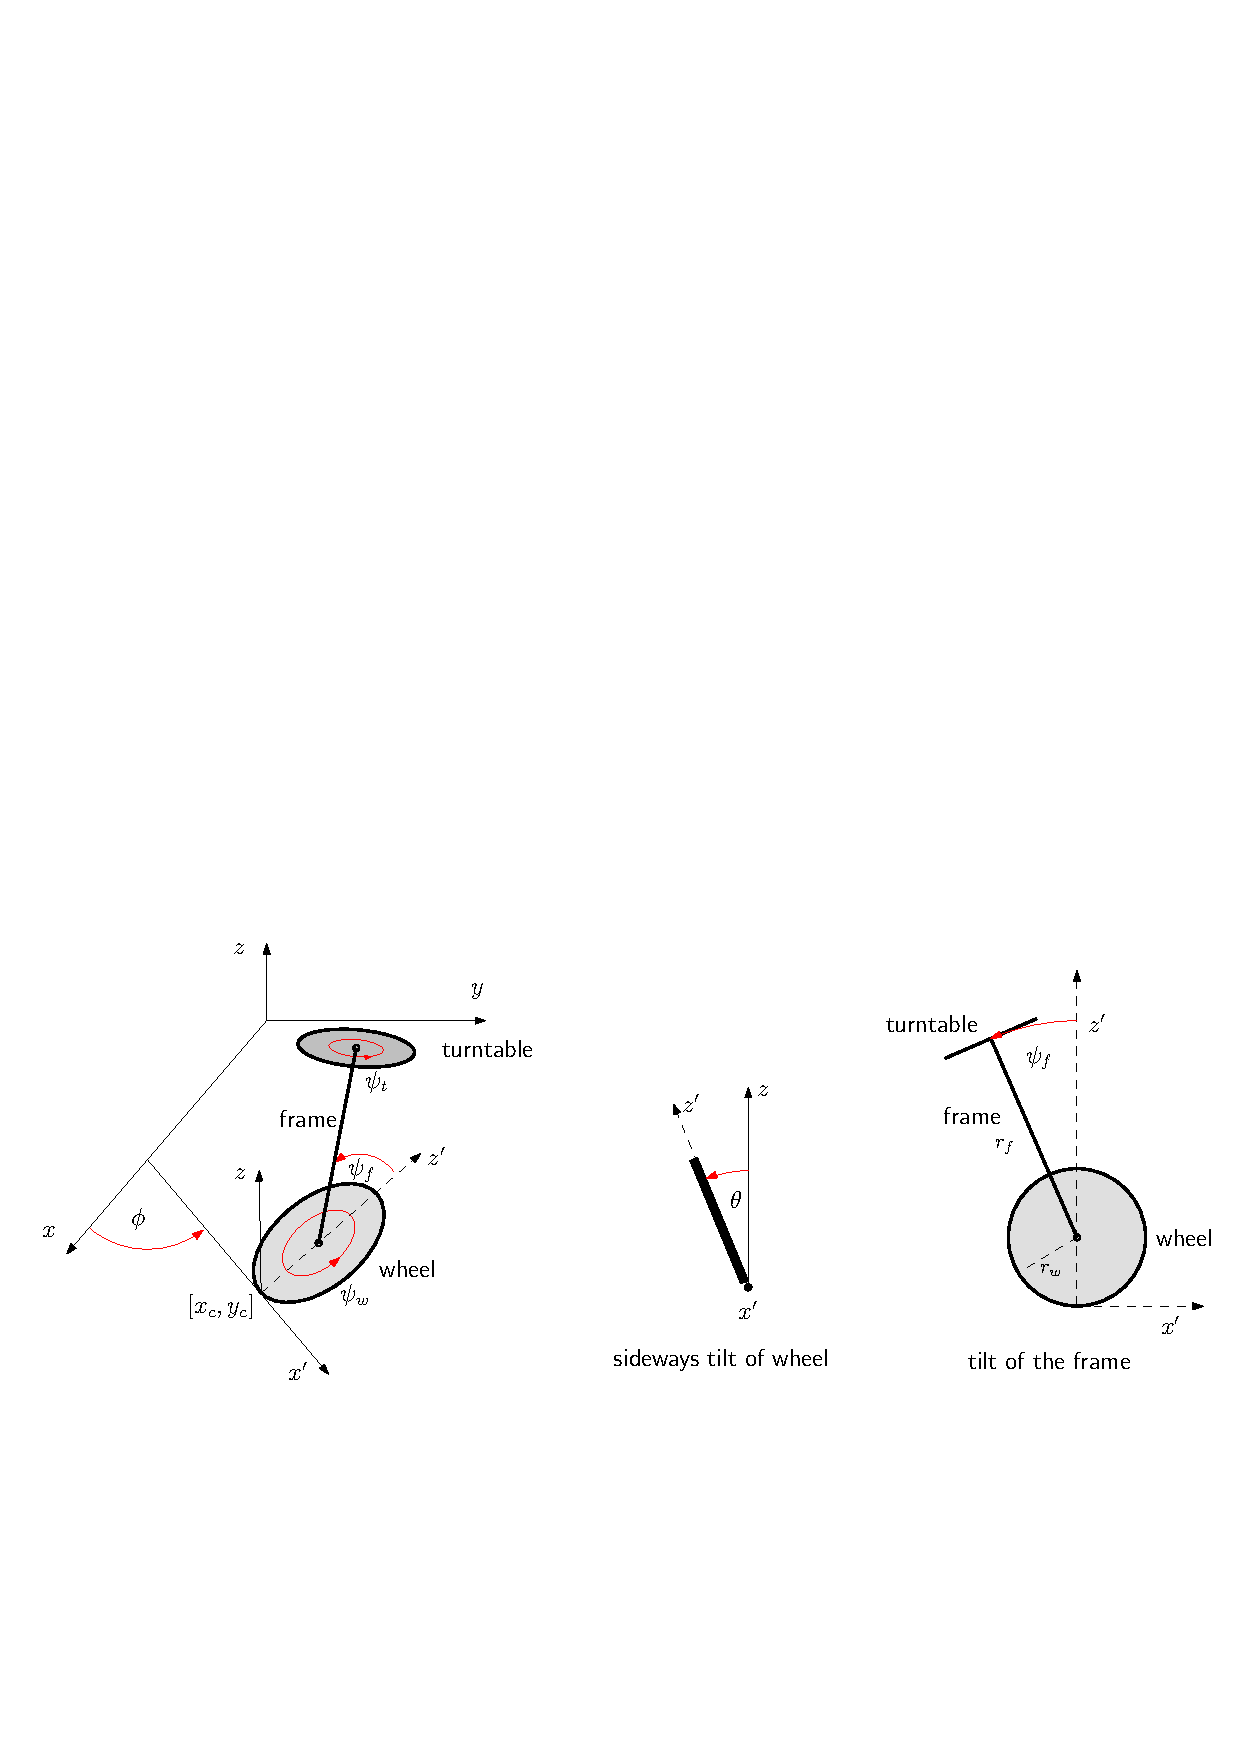
\includegraphics[height = 5cm]{./figures/unicycle}
\caption{Unicycle.}
\label{fig:unicycle}
\end{figure}
%
A sketch of the unicycle system is shown in
Figure~\ref{fig:unicycle}. The equations of motion that govern the
unicycle were derived in the MSc thesis by
Forster~\cite{Forster2009}. We shall provide a sketch of the full
derivation here, in which we follow the steps taken by
Forster~\cite{Forster2009}, Section 3.3.



\subsection{Method}
%-------------------------------------------------------------------------------------------------------------------------------------------
\begin{figure}[tb]
\centering
%set the plot display orientation
%synatax: \tdplotsetdisplay{\theta_d}{\phi_d}
\tdplotsetmaincoords{65}{100}

%define polar coordinates for some vector
%TODO: look into using 3d spherical coordinate system
\pgfmathsetmacro{\magW}{4}
\pgfmathsetmacro{\psiW}{-30}
\pgfmathsetmacro{\theW}{10}
\pgfmathsetmacro{\phiW}{15}

%start tikz picture, and use the tdplot_main_coords style to implement the display 
%coordinate transformation provided by 3dplot
\footnotesize
\begin{tikzpicture}[scale=0.85,tdplot_main_coords]

%set up some coordinates ... GET FROM MATLAB
%-----------------------
\coordinate (O) at (1.7321,-1,0);
\coordinate (B) at (2.5,4.3301,0);
\coordinate (Bp) at (4.2321,3.3301,0);
\coordinate (W) at (2.7256,4.1999,1.4772);
\coordinate (Wt) at (3.1767,3.9394,4.4316);
\coordinate (Wtp) at (2.7256,4.1999,4.4316);
\coordinate (Wbp) at (2.7256,4.1999,0);
\coordinate (T) at (2.7969,2.8138,5.7578);
\coordinate (F) at (2.7612,3.5069,3.6175);

%draw figure contents
%--------------------

%draw the main coordinate system axes
\tdplotsetrotatedcoordsorigin{(O)}
\tdplotsetrotatedcoords{0}{0}{0}
\draw[tdplot_rotated_coords,-latex,blue,thick] (0,0,0) -- (1.5,0,0)
node[anchor=south east]{$\vec i$};
\draw[tdplot_rotated_coords,-latex,blue,thick] (0,0,0) -- (0,1.5,0)
node[anchor=south]{$\vec j$};
\draw[tdplot_rotated_coords,-latex,blue,thick] (0,0,0) -- (0,0,1.5)
node[anchor=south]{$\vec k$};
\draw[dashed] (W) -- (Wt);
\draw[dashed] (Wtp) -- (Wbp);
\draw[dashed] (B) -- (W);

\draw[red,-latex] (B) -- (Bp);
\draw[red,-latex] (Bp) -- (O);
\node at (0,0.8,-1.7) {\color{red} $x_\te{c}$};
\node at (0,3.2,-1.4) {\color{red} $y_\te{c}$};
\tdplotsetrotatedcoords{\psiW}{0}{0}
\tdplotsetrotatedcoordsorigin{(Bp)}
\draw[tdplot_rotated_coords,very thin] (-0.35,0,0) -- (-0.35,-0.35,0) -- (0,-0.35,0);


% draw frame
\draw[very thick,black] (W) -- (T);
\tdplotsetrotatedcoords{\psiW}{100}{0}
\tdplotsetrotatedcoordsorigin{(F)}
\draw[tdplot_rotated_coords,fill=black] (0,0,0) circle (0.12);

% draw turntable
\tdplotsetrotatedcoords{\psiW}{\theW}{\phiW}
\tdplotsetrotatedcoordsorigin{(T)}
\draw[tdplot_rotated_coords,very thick,fill=black,fill opacity=0.2] (0,0,0) circle (1.5);
\draw[tdplot_rotated_coords,fill=black] (0,0,0) circle (0.12);
\tdplotdrawarcarrow[tdplot_rotated_coords,red]{(T)}{0.65}{0}{270}{}{}
\tdplotdrawarcarrow[tdplot_rotated_coords,blue]{(T)}{0.4}{0}{270}{}{}
\node at (0,3.25,4.8) {\color{red} $\psi_\te{t}$};
\node at (0,1.7,4.2) {\color{blue} $u_\te{t}$};

% draw wheel
\tdplotsetrotatedcoords{\psiW}{100}{0} % add 90 to j angle
\tdplotsetrotatedcoordsorigin{(W)}
\draw[tdplot_rotated_coords,very thick,fill=black,fill opacity=0.2] (0,0,0) circle (1.5);
\draw[tdplot_rotated_coords,fill=black] (0,0,0) circle (0.12);
\tdplotdrawarcarrow[tdplot_rotated_coords,red]{(W)}{0.6}{0}{270}{}{}
\tdplotdrawarcarrow[tdplot_rotated_coords,blue]{(W)}{0.4}{0}{270}{}{}
\node at (0,4.35,0.5) {\color{red} $\phi_\te{w}$};
\node at (0,3.3,-0.1) {\color{blue} $u_\te{w}$};



% show theta and phi
\tdplotdrawarcarrow[red]{(O)}{0.8}{0}{60}{anchor=north}{\color{red} $\psi$}
\tdplotsetrotatedcoords{\psiW}{190}{-90} % add 180 to j angle
\tdplotsetrotatedcoordsorigin{(W)}
\tdplotdrawarcarrow[tdplot_rotated_coords,red]{(W)}{2.8}{80}{90}{anchor=south}{\color{red} $\theta$}
\tdplotsetrotatedcoords{\psiW}{100}{0} % add 90 to j angle
\tdplotsetrotatedcoordsorigin{(W)}
\tdplotdrawarcarrow[tdplot_rotated_coords,red]{(W)}{2.8}{180}{195}{anchor=south}{\color{red} $\phi$}


\end{tikzpicture}

\caption{The robotic unicycle with state variables: pitch angle
  $\phi$, roll angle $\theta$, yaw angle $\psi$, wheel angle
  $\phi_\te{w}$, turntable angle $\psi_\te{t}$, the associated angular
  velocities and the location of the global origin
  $(x_\te{c},y_\te{c})$. The actions are the wheel motor torque
  $u_\te{w}$ and the turntable motor torque $u_\te{t}$. The global
  coordinate system is defined by the vectors $\vec i, \vec j$ and
  $\vec k$.}
\label{fig:unibody}
\end{figure}
%-------------------------------------------------------------------------------------------------------------------------------------------
The robotic unicycle is shown in Figure~\ref{fig:unibody} with global
coordinate system defined by the orthonormal vectors ${\vec i}, \vec j$ and
$\vec k$. The spatial position of the unicycle is fully defined by the
pitch angle $\phi$, roll angle $\theta$, yaw angle $\psi$, wheel angle
$\phi_\te{w}$, turntable angle $\psi_\te{t}$ and location of the
global origin with respect to the body-centred coordinate system
$(x_\te{c},y_\te{c})$. We chose the state vector to be $\vec x =
[\phi,\dot\phi,\theta,\dot\theta,\psi,\dot\psi,\dot\phi_\te{w},
\dot\psi_\te{t},x_\te{c},y_\te{c}]\T \in\R^{10}$ where we exclude
$\phi_\te{w}$ and $\psi_\te{t}$ since they clearly have no effect on
the dynamics. The action vector $\vec u$ is made up of a wheel motor
torque $u_\te{w}$ and a turntable motor torque $u_\te{t}$.  

Let us start with the coordinates $(x_\te{c},y_\te{c})$. These are
centred on the point of contact with the floor and define the location
of the global origin. The coordinate $x_\te{c}$ lies parallel to the
current direction of travel and $y_\te{c}$ is orthogonal to it. These
coordinates evolve according to
\begin{align}
\dot x_\te{c} &= r_\te{w} \dot\phi_\te{w} \cos\psi \label{eq:xceqn}  \\
\dot y_\te{c} &= r_\te{w} \dot\phi_\te{w} \sin\psi \label{eq:yceqn}
\end{align}
where $r_\te{w}$ is the wheel radius.  The full unicycle model was
obtained by analysing the wheel, frame and turntable as individual
Free Body Diagrams (FBDs), as depicted in Figure~\ref{fig:FBDs}. Linear momentum
and moment of momentum for each FBD were then resolved to yield six
scalar equations for each free body. The internal forces were then
eliminated to yield five independent scalar equations which govern the
evolution of the angular states. A description of the physical
constants of the system along with the values we use in this thesis
are given in Table~\ref{tab:uniconsts}.
%-------------------------------------------------------------------------------------------------------------------------------------------
\begin{table}
\renewcommand{\arraystretch}{1.3}
\begin{center}
%\setlength{\extrarowheight}{2pt}
\rowcolors{1}{black!10}{white}
\centerline{
\small
\begin{tabular}{c  l  c  c}
%\toprule[1.5pt] 
{\bf Constant} & {\bf Description} & {\bf Value} & {\bf Units } \\
\hline
$m_\te{w}$ & Wheel mass & 1.0 & kg \\
$r_\te{w}$ & Wheel radius & 0.225 & m \\
$A_\te{w}$ & Moment of inertia of wheel around $\vec i_\te{w}$ & 0.0242 & kg$\,$m$^2$ \\
$C_\te{w}$ & Moment of inertia of wheel around $\vec k_\te{w}$ & 0.0484 & kg$\,$m$^2$ \\
%
$m_\te{f}$ & Frame mass  & 23.5 & kg \\
$r_\te{f}$ & Frame centre of mass to wheel & 0.54 & m \\
$A_\te{f}$ & Moment of inertia of frame around $\vec i_\te{f}$ & 0.4248 & kg$\,$m$^2$ \\
$B_\te{f}$ & Moment of inertia of frame around $\vec j_\te{f}$ & 0.4608 & kg$\,$m$^2$ \\
$C_\te{f}$ & Moment of inertia of frame around $\vec k_\te{f}$ & 0.8292 & kg$\,$m$^2$ \\
%
$m_\te{t}$ & Turntable mass & 10.0 & kg \\
$r_\te{t}$ & Frame centre of mass to turntable & 0.27 & m \\
$A_\te{t}$ & Moment of inertia of turntable around $\vec i_\te{t}$ & 1.3 & kg$\,$m$^2$ \\
$C_\te{t}$ & Moment of inertia of turntable around $\vec k_\te{t}$ & 0.2 & kg$\,$m$^2$ \\
$g$ & Gravitational acceleration & 9.81 & m$\,$s$^{-2}$ \\
%\bottomrule[1.5pt]
\end{tabular}
}
\end{center}
\caption{Physical constants used for the simulated robotic
  unicycle. The coordinate systems defined by the $\vec i, \vec j$ and
  $\vec k$ vectors are shown in Figure~\ref{fig:FBDs}.}
\label{tab:uniconsts}
\end{table}
%-------------------------------------------------------------------------------------------------------------------------------------------


\subsection{Wheel FBD}
The wheel coordinate system is defined by the orthonormal vectors
$\vec i_\te{w},\vec j_\te{w}$ and $\vec k_\te{w}$ as shown in
Figure~\ref{fig:wheelFBD}. We begin by noting that the angular
velocity of the wheel coordinate system is $\Omega_\te{w} =
\dot\psi\vec k + \dot\theta\vec j_\te{w}$. Now noting that the angular
velocity of the wheel only differs in the $\vec k_\te{w}$ direction
and assuming no slip between wheel and floor we have expressions for
the velocity and angular velocity of the wheel
\begin{align*}
\vec v_\te{w} &= -(\vec\omega_\te{w}\times r_\te{w}\vec i_\te{w}) \\
\vec\omega_\te{w} &= \Omega_\te{w} + \dot\phi_\te{w}\vec k_\te{w}
\end{align*}
From these expressions we can derive the acceleration of the wheel
$\dot{\vec v}_\te{w}$ and the rate of change of angular momentum
$\dot{\vec h}_\te{w}$ as
\begin{align*}
  \dot{\vec v}_\te{w} &= \pdiff{\vec v_\te{w}}{t} + (\Omega_\te{w}\times
   \vec v_\te{w}) \\
   \dot{\vec h}_\te{w} &= A_\te{w}\pdiff{\omega_\te{w}[1]}{t}\vec i_\te{w} +
    A_\te{w}\pdiff{\omega_\te{w}[2]}{t}\vec j_\te{w} +
    C_\te{w}\pdiff{\omega_\te{w}[3]}{t}\vec k_\te{w} +
   (\Omega_\te{w}\times \vec h_\te{w})
\end{align*}
where angular momentum in the wheel frame of reference is $\vec h_\te{w}
= [A_\te{w}; A_\te{w}; C_\te{w}] \circ \vec\omega_\te{w}$.  Now we consider
the forces acting on the wheel free body. These are given by the
unknown quantities: axle force $F_\te{w}$, axle torque $Q_\te{w}$ \&
reaction force $R$ and the known quantities: wheel weight $W_\te{w}$
\& friction torque $T$. These forces and moments are shown in the
right-hand plot of Figure~\ref{fig:wheelFBD}. Note that we actually
know the component of the axle torque $Q_\te{w}$ in the $\vec
k_\te{w}$ direction as it is given by the reaction of the wheel motor
on the wheel itself $u_\te{w}$. Resolving the rate of change of linear
momentum and the rate of change of angular momentum around the center
of mass leads to
\begin{align}
  m_\te{w}\dot{\vec v}_\te{w} &= R + F_\te{w} + W_\te{w} \label{eq:wFBD1} \\
  \dot{\vec h}_\te{w} &= (r_\te{w}\vec i_\te{w} \times R) + Q_\te{w} +
  T \label{eq:wFBD2}
\end{align}


%-------------------------------------------------------------------------------------------------------------------------------------------
\begin{figure}
\centering
\subfigure[The wheel as a free body diagram and coordinate system defined by $\vec i_\te{w},\vec j_\te{w}$ and $\vec k_\te{w}$]{
%set the plot display orientation
%synatax: \tdplotsetdisplay{\theta_d}{\phi_d}
\tdplotsetmaincoords{65}{100}

%define polar coordinates for some vector
%TODO: look into using 3d spherical coordinate system
\pgfmathsetmacro{\magW}{4}
\pgfmathsetmacro{\psiW}{-30}
\pgfmathsetmacro{\theW}{10}
\pgfmathsetmacro{\phiW}{15}

%start tikz picture, and use the tdplot_main_coords style to implement the display 
%coordinate transformation provided by 3dplot
\footnotesize
\begin{tikzpicture}[scale=0.85,tdplot_main_coords]

%set up some coordinates ... GET FROM MATLAB
%-----------------------
\coordinate (O) at (1.7321,-1,0);
\coordinate (B) at (2.5,4.3301,0);
\coordinate (Bp) at (4.2321,3.3301,0);
\coordinate (W) at (2.7256,4.1999,1.4772);
\coordinate (Wt) at (3.1767,3.9394,4.4316);
\coordinate (Wtp) at (2.7256,4.1999,4.4316);
\coordinate (Wbp) at (2.7256,4.1999,0);
\coordinate (T) at (2.7969,2.8138,5.7578);
\coordinate (F) at (2.7612,3.5069,3.6175);

%draw figure contents
%--------------------

%draw the main coordinate system axes
\tdplotsetrotatedcoordsorigin{(O)}
\tdplotsetrotatedcoords{0}{0}{0}
\draw[tdplot_rotated_coords,-latex,blue,thick] (0,0,0) -- (1.5,0,0) node[anchor=south east]{${\vec i}$};
\draw[tdplot_rotated_coords,-latex,blue,thick] (0,0,0) -- (0,1.5,0) node[anchor=south]{$\vec j$};
\draw[tdplot_rotated_coords,-latex,blue,thick] (0,0,0) -- (0,0,1.5) node[anchor=south]{${\vec k}$};
\draw[dashed] (W) -- (Wt);
\draw[dashed] (Wtp) -- (Wbp);
\draw[dashed] (B) -- (W);
\draw[dashed] (B) -- (Bp) -- (O);

\tdplotsetrotatedcoords{\psiW}{0}{0}
\tdplotsetrotatedcoordsorigin{(Bp)}
\draw[tdplot_rotated_coords,very thin] (-0.35,0,0) -- (-0.35,-0.35,0) -- (0,-0.35,0);

% draw frame
\draw[very thick,black!30] (W) -- (T);
\tdplotsetrotatedcoords{\psiW}{100}{0}
\tdplotsetrotatedcoordsorigin{(F)}
\draw[tdplot_rotated_coords,fill=black!30,black!30] (0,0,0) circle (0.12);

% draw turntable
\tdplotsetrotatedcoords{\psiW}{\theW}{\phiW}
\tdplotsetrotatedcoordsorigin{(T)}
\draw[tdplot_rotated_coords,very thick,black!30,fill=black!30,fill opacity=0.2] (0,0,0) circle (1.5);
\draw[tdplot_rotated_coords,fill=black!30,black!30] (0,0,0) circle (0.12);

% draw wheel
\tdplotsetrotatedcoords{\psiW}{\theW}{0}
\tdplotsetrotatedcoordsorigin{(W)}
\draw[tdplot_rotated_coords,-latex,blue,thick] (0,0,0) -- (1.45,0,0); \node at (0,2.8,-0.8) {\color{blue}${\vec k}_\te{w}$};
\draw[tdplot_rotated_coords,-latex,blue,thick] (0,0,0) -- (0,1.45,0); \node at (0,5.2,-0.1) {\color{blue}$\vec j_\te{w}$};
\draw[tdplot_rotated_coords,-latex,blue,thick] (0,0,0) -- (0,0,-1.45); \node at (0,4,-1.5) {\color{blue}${\vec i}_\te{w}$};

\tdplotsetrotatedcoords{\psiW}{100}{0} % add 90 to j angle
\tdplotsetrotatedcoordsorigin{(W)}
\draw[tdplot_rotated_coords,very thick,fill=black,fill opacity=0.2] (0,0,0) circle (1.5);
\draw[tdplot_rotated_coords,fill=black] (0,0,0) circle (0.12);
\tdplotdrawarcarrow[tdplot_rotated_coords,red]{(W)}{0.5}{0}{270}{}{}
\node at (0,4.3,0.5) {\color{red} $\phi_\te{w}$};



% show theta and phi
\tdplotdrawarcarrow[red]{(O)}{0.8}{0}{60}{anchor=north}{\color{red} $\psi$}
\tdplotsetrotatedcoords{\psiW}{190}{-90} % add 180 to j angle
\tdplotsetrotatedcoordsorigin{(W)}
\tdplotdrawarcarrow[tdplot_rotated_coords,red]{(W)}{2.8}{80}{90}{anchor=south}{\color{red} $\theta$}
\tdplotsetrotatedcoords{\psiW}{100}{0} % add 90 to j angle
\tdplotsetrotatedcoordsorigin{(W)}
\tdplotdrawarcarrow[tdplot_rotated_coords,red]{(W)}{2.8}{180}{195}{anchor=south}{\color{red} $\phi$}


\end{tikzpicture}

%set the plot display orientation
%synatax: \tdplotsetdisplay{\theta_d}{\phi_d}
\tdplotsetmaincoords{65}{100}

%define polar coordinates for some vector
%TODO: look into using 3d spherical coordinate system
\pgfmathsetmacro{\magW}{4}
\pgfmathsetmacro{\psiW}{-30}
\pgfmathsetmacro{\theW}{10}
\pgfmathsetmacro{\phiW}{15}

%start tikz picture, and use the tdplot_main_coords style to implement the display 
%coordinate transformation provided by 3dplot
\footnotesize
\begin{tikzpicture}[scale=0.85,tdplot_main_coords]

%set up some coordinates ... GET FROM MATLAB
%-----------------------
\coordinate (O) at (1.7321,-1,0);
\coordinate (B) at (2.5,4.3301,0);
\coordinate (Bp) at (4.2321,3.3301,0);
\coordinate (W) at (2.7256,4.1999,1.4772);
\coordinate (Wt) at (3.1767,3.9394,4.4316);
\coordinate (Wtp) at (2.7256,4.1999,4.4316);
\coordinate (Wbp) at (2.7256,4.1999,0);
\coordinate (T) at (2.7969,2.8138,5.7578);
\coordinate (F) at (2.7612,3.5069,3.6175);

%draw figure contents
%--------------------


% draw frame
\draw[very thick,black!30] (W) -- (T);
\tdplotsetrotatedcoords{\psiW}{100}{0}
\tdplotsetrotatedcoordsorigin{(F)}
\draw[tdplot_rotated_coords,fill=black!30,black!30] (0,0,0) circle (0.12);

% draw turntable
\tdplotsetrotatedcoords{\psiW}{\theW}{\phiW}
\tdplotsetrotatedcoordsorigin{(T)}
\draw[tdplot_rotated_coords,very thick,black!30,fill=black!30,fill opacity=0.2] (0,0,0) circle (1.5);
\draw[tdplot_rotated_coords,fill=black!30,black!30] (0,0,0) circle (0.12);

% draw wheel
\tdplotsetrotatedcoords{\psiW}{\theW}{0}
\tdplotsetrotatedcoordsorigin{(W)}

\tdplotsetrotatedcoords{\psiW}{100}{0} % add 90 to j angle
\draw[tdplot_rotated_coords,very thick,fill=black,fill opacity=0.2] (0,0,0) circle (1.5);
\draw[tdplot_rotated_coords,fill=black] (0,0,0) circle (0.12);

% draw forces and moments
\tdplotdrawarcarrow[red,thick,dashed]{(W)}{0.5}{50}{360}{}{}
\tdplotsetrotatedcoords{0}{0}{0}
\draw[tdplot_rotated_coords,thick,-latex,red,dashed] (0,0.8,0.8) -- (0,0.05,0.05);
\draw[tdplot_rotated_coords,thick,-latex,red] (0,0,-0.12) -- (0,0,-1.1);

\tdplotdrawarcarrow[red,thick]{(B)}{0.5}{50}{360}{}{}
\tdplotsetrotatedcoordsorigin{(B)}
\draw[tdplot_rotated_coords,thick,-latex,red,dashed] (0,0.8,0.8) -- (0,0.05,0.05);

\node at (0,4.0,0.85) {\color{red}$F_\te{w}$};
\node at (0,3.2,0.55) {\color{red}$Q_\te{w}$};
\node at (0,4.3,-0.4) {\color{red}$R$};
\node at (0,3.2,-1.2) {\color{red}$T$};
\node at (0,3.4,-0.45) {\color{red}$W_\te{w}$};

\end{tikzpicture}

\label{fig:wheelFBD}
}
\subfigure[The frame as a free body diagram and coordinate system defined by $\vec i_\te{f},\vec j_\te{f}$ and $\vec k_\te{f}$]{
%set the plot display orientation
%synatax: \tdplotsetdisplay{\theta_d}{\phi_d}
\tdplotsetmaincoords{65}{100}

%define polar coordinates for some vector
%TODO: look into using 3d spherical coordinate system
\pgfmathsetmacro{\magW}{4}
\pgfmathsetmacro{\psiW}{-30}
\pgfmathsetmacro{\theW}{10}
\pgfmathsetmacro{\phiW}{15}

%start tikz picture, and use the tdplot_main_coords style to implement the display 
%coordinate transformation provided by 3dplot
\footnotesize
\begin{tikzpicture}[scale=0.85,tdplot_main_coords]

%set up some coordinates ... GET FROM MATLAB
%-----------------------
\coordinate (O) at (1.7321,-1,0);
\coordinate (B) at (2.5,4.3301,0);
\coordinate (Bp) at (4.2321,3.3301,0);
\coordinate (W) at (2.7256,4.1999,1.4772);
\coordinate (Wt) at (3.1767,3.9394,4.4316);
\coordinate (Wtp) at (2.7256,4.1999,4.4316);
\coordinate (Wbp) at (2.7256,4.1999,0);
\coordinate (T) at (2.7969,2.8138,5.7578);
\coordinate (F) at (2.7612,3.5069,3.6175);

%draw figure contents
%--------------------

%draw the main coordinate system axes
\tdplotsetrotatedcoordsorigin{(O)}
\tdplotsetrotatedcoords{0}{0}{0}
\draw[tdplot_rotated_coords,-latex,blue,thick] (0,0,0) -- (1.5,0,0) node[anchor=south east]{$\vec i$};
\draw[tdplot_rotated_coords,-latex,blue,thick] (0,0,0) -- (0,1.5,0) node[anchor=south]{$\vec j$};
\draw[tdplot_rotated_coords,-latex,blue,thick] (0,0,0) -- (0,0,1.5) node[anchor=south]{$\vec k$};
\draw[dashed] (W) -- (Wt);
\draw[dashed] (Wtp) -- (Wbp);
\draw[dashed] (B) -- (W);
\draw[dashed] (B) -- (Bp) -- (O);

\tdplotsetrotatedcoords{\psiW}{0}{0}
\tdplotsetrotatedcoordsorigin{(Bp)}
\draw[tdplot_rotated_coords,very thin] (-0.35,0,0) -- (-0.35,-0.35,0) -- (0,-0.35,0);

% draw wheel
\tdplotsetrotatedcoords{\psiW}{100}{0} % add 90 to j angle
\tdplotsetrotatedcoordsorigin{(W)}
\draw[tdplot_rotated_coords,very thick,black!30,fill=black!30,fill opacity=0.2] (0,0,0) circle (1.5);
\draw[tdplot_rotated_coords,fill=black] (0,0,0) circle (0.12);

% draw frame
\draw[very thick,black] (W) -- (T);
\tdplotsetrotatedcoords{\psiW}{\theW}{\phiW}
\tdplotsetrotatedcoordsorigin{(F)}
\draw[tdplot_rotated_coords,-latex,blue,thick] (0,0,0) -- (1.45,0,0); \node at (0,2.0,1.75) {\color{blue}$\vec k_\te{f}$};
\draw[tdplot_rotated_coords,-latex,blue,thick] (0,0,0) -- (0,1.45,0); \node at (0,4.3,2.5) {\color{blue}$\vec j_\te{f}$};
\draw[tdplot_rotated_coords,-latex,blue,thick] (0,0,0) -- (0,0,-1.45); \node at (0,3.25,0.85) {\color{blue}$\vec i_\te{f}$};
\tdplotsetrotatedcoords{\psiW}{100}{0}
\draw[tdplot_rotated_coords,fill=black] (0,0,0) circle (0.12);

% draw turntable
\tdplotsetrotatedcoords{\psiW}{\theW}{\phiW}
\tdplotsetrotatedcoordsorigin{(T)}
\draw[tdplot_rotated_coords,very thick,black!30,fill=black!30,fill opacity=0.2] (0,0,0) circle (1.5);
\draw[tdplot_rotated_coords,fill=black] (0,0,0) circle (0.12);



% show theta and phi
\tdplotdrawarcarrow[red]{(O)}{0.8}{0}{60}{anchor=north}{\color{red} $\psi$}
\tdplotsetrotatedcoords{\psiW}{190}{-90} % add 180 to j angle
\tdplotsetrotatedcoordsorigin{(W)}
\tdplotdrawarcarrow[tdplot_rotated_coords,red]{(W)}{2.8}{80}{90}{anchor=south}{\color{red} $\theta$}
\tdplotsetrotatedcoords{\psiW}{100}{0} % add 90 to j angle
\tdplotsetrotatedcoordsorigin{(W)}
\tdplotdrawarcarrow[tdplot_rotated_coords,red]{(W)}{2.8}{180}{195}{anchor=south}{\color{red} $\phi$}



\end{tikzpicture}

%set the plot display orientation
%synatax: \tdplotsetdisplay{\theta_d}{\phi_d}
\tdplotsetmaincoords{65}{100}

%define polar coordinates for some vector
%TODO: look into using 3d spherical coordinate system
\pgfmathsetmacro{\magW}{4}
\pgfmathsetmacro{\psiW}{-30}
\pgfmathsetmacro{\theW}{10}
\pgfmathsetmacro{\phiW}{15}

%start tikz picture, and use the tdplot_main_coords style to implement the display 
%coordinate transformation provided by 3dplot
\footnotesize
\begin{tikzpicture}[scale=0.85,tdplot_main_coords]

%set up some coordinates ... GET FROM MATLAB
%-----------------------
\coordinate (O) at (0,0,0);

\coordinate (B) at (3,5.1962,0);
\coordinate (W) at (3.2256,5.0659,1.4772);
\coordinate (Wt) at (3.6767,4.8054,4.4316);
\coordinate (Wtp) at (3.2256,5.0659,4.4316);
\coordinate (Wbp) at (3.2256,5.0659,0);
\coordinate (T) at (3.2969,3.6799,5.7578);
\coordinate (F) at (3.2612,4.3729,3.6175);

%draw figure contents
%--------------------


% draw wheel
\tdplotsetrotatedcoords{\psiW}{100}{0} % add 90 to j angle
\tdplotsetrotatedcoordsorigin{(W)}
\draw[tdplot_rotated_coords,very thick,black!30,fill=black!30,fill opacity=0.2] (0,0,0) circle (1.5);
\draw[tdplot_rotated_coords,fill=black] (0,0,0) circle (0.12);

% draw frame
\draw[very thick,black] (W) -- (T);
\tdplotsetrotatedcoordsorigin{(F)}
\tdplotsetrotatedcoords{\psiW}{100}{0}
\draw[tdplot_rotated_coords,fill=black] (0,0,0) circle (0.12);

% draw turntable
\tdplotsetrotatedcoords{\psiW}{\theW}{\phiW}
\tdplotsetrotatedcoordsorigin{(T)}
\draw[tdplot_rotated_coords,very thick,black!30,fill=black!30,fill opacity=0.2] (0,0,0) circle (1.5);
\draw[tdplot_rotated_coords,fill=black] (0,0,0) circle (0.12);

% draw forces and moments
\tdplotdrawarcarrow[red,thick,dashed]{(W)}{0.5}{50}{360}{}{}
\tdplotsetrotatedcoords{0}{0}{0}
\tdplotsetrotatedcoordsorigin{(W)}
\draw[tdplot_rotated_coords,thick,-latex,red,dashed] (0,0.8,0.8) -- (0,0.05,0.05);

\tdplotdrawarcarrow[red,thick,dashed]{(T)}{0.5}{50}{360}{}{}
\tdplotsetrotatedcoords{0}{0}{0}
\tdplotsetrotatedcoordsorigin{(T)}
\draw[tdplot_rotated_coords,thick,-latex,red,dashed] (0,0.8,0.8) -- (0,0.05,0.05);

\tdplotsetrotatedcoordsorigin{(F)}
\draw[tdplot_rotated_coords,thick,-latex,red] (0,0,-0.12) -- (0,0,-1.2);

\node at (0,3.5,1.5) {\color{red}$W_\te{f}$};
\node at (0,4,4.7) {\color{red}$G_\te{f}$};
\node at (0,2.3,4) {\color{red}$P_\te{f}$};
\node at (0,4.8,0.65) {\color{red}$F_\te{f}$};
\node at (0,3.95,0.25) {\color{red}$Q_\te{f}$};

\end{tikzpicture}

\label{fig:frameFBD}
}
\subfigure[The turntable as a free body diagram and coordinate system defined by $\vec i_\te{t},\vec j_\te{t}$ and $\vec k_\te{t}$]{
%set the plot display orientation
%synatax: \tdplotsetdisplay{\theta_d}{\phi_d}
\tdplotsetmaincoords{65}{100}

%define polar coordinates for some vector
%TODO: look into using 3d spherical coordinate system
\pgfmathsetmacro{\magW}{4}
\pgfmathsetmacro{\psiW}{-30}
\pgfmathsetmacro{\theW}{10}
\pgfmathsetmacro{\phiW}{15}

%start tikz picture, and use the tdplot_main_coords style to implement the display 
%coordinate transformation provided by 3dplot
\footnotesize
\begin{tikzpicture}[scale=0.85,tdplot_main_coords]

%set up some coordinates ... GET FROM MATLAB
%-----------------------
\coordinate (O) at (1.7321,-1,0);
\coordinate (B) at (2.5,4.3301,0);
\coordinate (Bp) at (4.2321,3.3301,0);
\coordinate (W) at (2.7256,4.1999,1.4772);
\coordinate (Wt) at (3.1767,3.9394,4.4316);
\coordinate (Wtp) at (2.7256,4.1999,4.4316);
\coordinate (Wbp) at (2.7256,4.1999,0);
\coordinate (T) at (2.7969,2.8138,5.7578);
\coordinate (F) at (2.7612,3.5069,3.6175);

%draw figure contents
%--------------------

%draw the main coordinate system axes
\tdplotsetrotatedcoordsorigin{(O)}
\tdplotsetrotatedcoords{0}{0}{0}
\draw[tdplot_rotated_coords,-latex,blue,thick] (0,0,0) -- (1.5,0,0)
node[anchor=south east]{$\vec i$};
\draw[tdplot_rotated_coords,-latex,blue,thick] (0,0,0) -- (0,1.5,0)
node[anchor=south]{$\vec j$};
\draw[tdplot_rotated_coords,-latex,blue,thick] (0,0,0) -- (0,0,1.5) node[anchor=south]{$\vec k$};
\draw[dashed] (W) -- (Wt);
\draw[dashed] (Wtp) -- (Wbp);
\draw[dashed] (B) -- (W);
\draw[dashed] (B) -- (Bp) -- (O);

\tdplotsetrotatedcoords{\psiW}{0}{0}
\tdplotsetrotatedcoordsorigin{(Bp)}
\draw[tdplot_rotated_coords,very thin] (-0.35,0,0) -- (-0.35,-0.35,0) -- (0,-0.35,0);

% draw wheel
\tdplotsetrotatedcoords{\psiW}{100}{0} % add 90 to j angle
\tdplotsetrotatedcoordsorigin{(W)}
\draw[tdplot_rotated_coords,very thick,black!30,fill=black!30,fill opacity=0.2] (0,0,0) circle (1.5);
\draw[tdplot_rotated_coords,fill=black!30,black!30] (0,0,0) circle (0.12);

% draw frame
\draw[very thick,black!30] (W) -- (T);
\tdplotsetrotatedcoords{\psiW}{\theW}{\phiW}
\tdplotsetrotatedcoordsorigin{(F)}
\tdplotsetrotatedcoords{\psiW}{100}{0}
\draw[tdplot_rotated_coords,fill=black!30,black!30] (0,0,0) circle (0.12);

% draw turntable
\tdplotsetrotatedcoords{\psiW}{\theW}{\phiW}
\tdplotsetrotatedcoordsorigin{(T)}
\draw[tdplot_rotated_coords,very thick,fill=black,fill opacity=0.2] (0,0,0) circle (1.5);
\draw[tdplot_rotated_coords,-latex,blue,thick] (0,0,0) -- (1.45,0,0);
\node at (0,1.5,3.3) {\color{blue}$\vec i_\te{t}$};
\draw[tdplot_rotated_coords,-latex,blue,thick] (0,0,0) -- (0,1.45,0);
\node at (0,3.65,4.3) {\color{blue}$\vec j_\te{t}$};
\draw[tdplot_rotated_coords,-latex,blue,thick] (0,0,0) -- (0,0,1.45); \node at (0,2.3,5.7) {\color{blue}$\vec k_\te{t}$};
\draw[tdplot_rotated_coords,fill=black] (0,0,0) circle (0.12);
\tdplotdrawarcarrow[tdplot_rotated_coords,red]{(T)}{0.5}{0}{270}{}{}
\node at (0,3.1,4.8) {\color{red} $\psi_\te{t}$};



% show theta and phi
\tdplotdrawarcarrow[red]{(O)}{0.8}{0}{60}{anchor=north}{\color{red} $\psi$}
\tdplotsetrotatedcoords{\psiW}{190}{-90} % add 180 to j angle
\tdplotsetrotatedcoordsorigin{(W)}
\tdplotdrawarcarrow[tdplot_rotated_coords,red]{(W)}{2.8}{80}{90}{anchor=south}{\color{red} $\theta$}
\tdplotsetrotatedcoords{\psiW}{100}{0} % add 90 to j angle
\tdplotsetrotatedcoordsorigin{(W)}
\tdplotdrawarcarrow[tdplot_rotated_coords,red]{(W)}{2.8}{180}{195}{anchor=south}{\color{red} $\phi$}



\end{tikzpicture}
%set the plot display orientation
%synatax: \tdplotsetdisplay{\theta_d}{\phi_d}
\tdplotsetmaincoords{65}{100}

%define polar coordinates for some vector
%TODO: look into using 3d spherical coordinate system
\pgfmathsetmacro{\magW}{4}
\pgfmathsetmacro{\psiW}{-30}
\pgfmathsetmacro{\theW}{10}
\pgfmathsetmacro{\phiW}{15}

%start tikz picture, and use the tdplot_main_coords style to implement the display 
%coordinate transformation provided by 3dplot
\footnotesize
\begin{tikzpicture}[scale=0.85,tdplot_main_coords]

%set up some coordinates ... GET FROM MATLAB
%-----------------------
\coordinate (O) at (0,0,0);

\coordinate (B) at (3,5.1962,0);
\coordinate (W) at (3.2256,5.0659,1.4772);
\coordinate (Wt) at (3.6767,4.8054,4.4316);
\coordinate (Wtp) at (3.2256,5.0659,4.4316);
\coordinate (Wbp) at (3.2256,5.0659,0);
\coordinate (T) at (3.2969,3.6799,5.7578);
\coordinate (F) at (3.2612,4.3729,3.6175);

%draw figure contents
%--------------------


% draw wheel
\tdplotsetrotatedcoords{\psiW}{100}{0} % add 90 to j angle
\tdplotsetrotatedcoordsorigin{(W)}
\draw[tdplot_rotated_coords,very thick,black!30,fill=black!30,fill opacity=0.2] (0,0,0) circle (1.5);
\draw[tdplot_rotated_coords,fill=black!30,black!30] (0,0,0) circle (0.12);

% draw frame
\draw[very thick,black!30] (W) -- (T);
\tdplotsetrotatedcoordsorigin{(F)}
\tdplotsetrotatedcoords{\psiW}{100}{0}
\draw[tdplot_rotated_coords,black!30,fill=black!30] (0,0,0) circle (0.12);

% draw turntable
\tdplotsetrotatedcoords{\psiW}{\theW}{\phiW}
\tdplotsetrotatedcoordsorigin{(T)}
\draw[tdplot_rotated_coords,very thick,fill=black,fill opacity=0.2] (0,0,0) circle (1.5);
\draw[tdplot_rotated_coords,fill=black] (0,0,0) circle (0.12);

% draw forces and moments
\tdplotdrawarcarrow[red,thick,dashed]{(T)}{0.5}{50}{360}{}{}
\tdplotsetrotatedcoords{0}{0}{0}
\tdplotsetrotatedcoordsorigin{(T)}
\draw[tdplot_rotated_coords,thick,-latex,red,dashed] (0,0.8,0.8) -- (0,0.05,0.05);
\draw[tdplot_rotated_coords,thick,-latex,red] (0,0,-0.06) -- (0,0,-1.2);

\node at (0,2.9,2.9) {\color{red}$W_\te{t}$};
\node at (0,4,4.7) {\color{red}$G_\te{t}$};
\node at (0,2.3,4) {\color{red}$P_\te{t}$};

\end{tikzpicture}

\label{fig:turntableFBD}
}
\caption{Free body diagrams of the wheel, frame and turntable of the unicycle. The model has the angular state variables pitch $\phi$, roll $\theta$, yaw $\psi$, wheel angle $\phi_\te{w}$ and turntable angle $\psi_\te{t}$. The vectors $\vec i, \vec j$ and $\vec k$ define the global fixed frame of reference. The centres of mass for each component are shown by the black dots. Forces and moments are shown on the right, with unknown quantities as dashed lines.}
\label{fig:FBDs}
\end{figure}
%-------------------------------------------------------------------------------------------------------------------------------------------







\subsection{Frame FBD}
The frame coordinate system is defined by the orthonormal vectors $\vec i_\te{f},\vec j_\te{f}$ and $\vec k_\te{f}=\vec k_\te{w}$ as shown in Figure~\ref{fig:frameFBD}. In this case, the angular velocity of the frame $\vec\omega_\te{f}$ is given by the angular velocity of the wheel plus an additional spin about the wheel axis and the velocity of the frame $\vec v_\te{f}$ is given by the velocity of the wheel plus an additional rotation about the wheel centre
\begin{align*}
\vec v_\te{f} &= \vec v_\te{w} -(\vec\omega_\te{f}\times r_\te{f}\vec i_\te{f}) \\
\vec\omega_\te{f} &= \Omega_\te{w} + \dot\phi\vec k_\te{f}
\end{align*}
As before, we can now derive the acceleration of the frame $\dot{\vec v}_\te{f}$ and the rate of change of angular momentum $\dot{\vec h}_\te{f}$ as
\begin{align*}
\dot{\vec v}_\te{f} &= \pdiff{{\vec v}_\te{f}}{t} + (\Omega_\te{f}\times {\vec v}_\te{f}) \\
\dot{\vec h}_\te{f} &= A_\te{f}\pdiff{\omega_\te{f}[1]}{t}\vec i_\te{f} + B_\te{f}\pdiff{\omega_\te{f}[2]}{t}\vec j_\te{f} + C_\te{f}\pdiff{\omega_\te{f}[3]}{t}\vec k_\te{f} +  (\Omega_\te{f}\times {\vec h}_\te{f})
\end{align*}
where angular momentum of the frame in this frame of reference is ${\vec h}_\te{f} = [A_\te{f}; B_\te{f}; C_\te{f}] \circ \vec\omega_\te{f}$. The forces and moments acting on the frame are shown on the right in Figure~\ref{fig:frameFBD}. They consist of the known frame weight $W_\te{f}$ and the unknown: wheel axle force $F_\te{f}=-F_\te{w}$, wheel axle torque $Q_\te{f}=-Q_\te{w}$, turntable axle force $G_\te{f}$ \& turntable axle torque $P_\te{f}$. But again we know that the dimension of $P_\te{f}$ acting along $\vec i_\te{f}$ is given by the reaction of the frame to the turntable motor $u_\te{t}$.  So resolving the rate of change of linear momentum and the rate of change of angular momentum around the centre of mass gives us
\begin{align}
m_\te{f}\dot{\vec v}_\te{f} &= F_\te{f} + G_\te{f} + W_\te{f} \label{eq:fFBD1} \\
\dot{\vec h}_\te{f} &= (r_\te{f}\vec i_\te{f} \times F_\te{f}) - (r_\te{t}\vec i_\te{f} \times G_\te{f}) + Q_\te{f} + P_\te{f} \label{eq:fFBD2} 
\end{align}


\subsection{Turntable FBD}
Finally, the turntable coordinate system is defined by the orthonormal vectors $\vec i_\te{t} = \vec k_\te{f},\vec j_\te{t} = \vec j_\te{f}$ and $\vec k_\te{t} = -\vec i_\te{f}$  as shown in Figure~\ref{fig:turntableFBD}. The velocity of the turntable centre ${\vec v}_\te{t}$ is equal to the velocity of the wheel plus an additiona lterm caused by rotation about the wheel centre, while the angular velocity $\vec\omega_\te{t}$ differs from $\Omega_\te{t}=\Omega_\te{f}$ only along $\vec k_\te{t}$ 
\begin{align*}
{\vec v}_\te{t} &= {\vec v}_\te{w} + (\Omega_\te{t}\times r\vec k_\te{t}) \\
\vec\omega_\te{t} &= \Omega_\te{t} + \dot\psi_\te{t}\vec k_\te{t}
\end{align*}
Again, we derive the acceleration of the frame $\dot{\vec v}_\te{t}$ and the rate of change of angular momentum $\dot{\vec h}_\te{t}$ as
\begin{align*}
\dot{\vec v}_\te{t} &= \pdiff{{\vec v}_\te{f}}{t} + (\Omega_\te{f}\times {\vec v}_\te{f}) \\
\dot{\vec h}_\te{t} &= A_\te{t}\pdiff{\omega_\te{t}[1]}{t}\vec i_\te{t} + A_\te{t}\pdiff{\omega_\te{t}[2]}{t}\vec j_\te{t} + C_\te{t}\pdiff{\omega_\te{t}[3]}{t}\vec k_\te{t} +  (\Omega_\te{t}\times {\vec h}_\te{t})
\end{align*}
where ${\vec h}_\te{t} = [A_\te{t}; A_\te{t}; C_\te{t}] \circ \vec\omega_\te{t}$. The forces and moments acting on the turntable lead to the last of our equations
\begin{align}
m_\te{t}\dot{\vec v}_\te{t} &= G_\te{t} + W_\te{t} \label{eq:tFBD1} \\
\dot{\vec h}_\te{t} &= P_\te{t} \label{eq:tFBD2} 
\end{align}





\subsection{Eliminating Internal Forces}
We now have 18 kinematic relationships given by
Equations~\eqref{eq:wFBD1}--\eqref{eq:tFBD2} which govern the
dynamics of the unicycle. These can be reduced to five expressions by
eliminating the 13 scalar unknowns found in the unknown internal
forces, $F$ and $G$, the unknown reaction force $R$ and the partially
unkown torques $Q$ and $P$. The first can be obtained from
Equation~\eqref{eq:tFBD2} and noting that the component of $P_\te{f}$
about $\vec k_\te{t}$ is the reaction to the motor torque $u_\te{t}$
\begin{align}
\dot{\vec h}_\te{t}\T\vec k_\te{t} &= u_\te{t} \label{eq:uniE1} 
\end{align}
The second can be obtained by first making use of the relationships
$G_\te{f}=-G_\te{t}$ \& $P_\te{f}=-P_\te{t}$ and then rearranging
Equation~\eqref{eq:fFBD1}, Equation~\eqref{eq:tFBD1} and Equation~\eqref{eq:tFBD2} to get
\begin{align*}
  F_\te{f} &= m_\te{t}\dot{\vec v}_\te{t} + m_\te{f}\dot{\vec v}_\te{f} -W_\te{t} - W_\te{f} \\
  G_\te{f} &= W_\te{t} - m_\te{t}\dot{\vec v}_\te{t} \\
  P_\te{f} &= -\dot{\vec h}_\te{t}
\end{align*}
Substituting these into Equation~\eqref{eq:fFBD2} and noting that $Q_\te{w}=-Q_\te{f}$ gives us
\begin{align*}
Q_\te{w} &= -\dot{\vec h}_\te{f} -\dot{\vec h}_\te{t} - \Big( r_\te{f}\vec i_\te{f} \times (W_\te{f}+W_\te{t} - m_\te{f}\dot{\vec v}_\te{f} - m_\te{t}\dot{\vec v}_\te{t}) \Big) - \Big(r_\te{t}\vec i_\te{f} \times (W_\te{t}-m_\te{t}\dot{\vec v}_\te{t})\Big)
\end{align*}
Once again, the component of $Q_\te{w}$ about the wheel axis is equal to the torque provided by the wheel motor $u_\te{w}$, therefore $Q_\te{w}\T\vec k_\te{w} = u_\te{w}$ and we have our second expression
\begin{align}
-\bigg(\dot{\vec h}_\te{f} +\dot{\vec h}_\te{t} + \Big( r_\te{f}\vec i_\te{f} \times (W_\te{f}+W_\te{t} - m_\te{f}\dot{\vec v}_\te{f} - m_\te{t}\dot{\vec v}_\te{t}) \Big) + \Big(r_\te{t}\vec i_\te{f} \times (W_\te{t}-m_\te{t}\dot{\vec v}_\te{t})\Big) \bigg)\T \vec k_\te{w} = u_\te{w}
 \label{eq:uniE2} 
\end{align}
Finally, Equation~\eqref{eq:wFBD1} can be combined with our expression for $F_\te{f}=-F_\te{w}$ to find the reaction force at the base
\begin{equation*}
R = m_\te{w}\dot{\vec v}_\te{w} + m_\te{f}\dot{\vec v}_\te{f} + m_\te{t}\dot{\vec v}_\te{t} -W_\te{w} - W_\te{f} - W_\te{t}
\end{equation*}
and can be substituted into Equation~\eqref{eq:wFBD2} to obtain the following three relationships
\begin{align}
  \dot{\vec h}_\te{w} &= \Big(r_\te{w}{\vec i}_\te{w} \times (m_\te{w}\dot{\vec v}_\te{w} + m_\te{f}\dot{\vec v}_\te{f} + m_\te{t}\dot{\vec v}_\te{t} -W_\te{w} - W_\te{f} - W_\te{t}) \Big) \label{eq:uniE3} \\
  \nonumber & \quad-\bigg(\dot{\vec h}_\te{f} +\dot{\vec h}_\te{t} + \Big(
  r_\te{f}\vec i_\te{f} \times (W_\te{f}+W_\te{t} - m_\te{f}\dot{\vec
    v}_\te{f} - m_\te{t}\dot{\vec v}_\te{t}) \Big) + \Big(r_\te{t}\vec
  i_\te{f} \times (W_\te{t}-m_\te{t}\dot{\vec v}_\te{t})\Big) \bigg) +
  T
\end{align}
The five expressions contained in
Equations~\eqref{eq:uniE1}--\eqref{eq:uniE3} form the foundation for
the model we use. The only unknowns remaining in these relationships
are the states: $\phi, \dot\phi, \theta, \dot\theta, \dot\psi,
\dot\phi_\te{w}, \dot\psi_\te{t}$, the torque actions: $u_\te{w},
u_\te{t}$ and the accelerations:
$\ddot\phi,\ddot\theta,\ddot\psi,\ddot\phi_\te{w},
\ddot\psi_\te{t}$. The equations were then rearranged by Forster,
through use of the Symbolic Toolbox in MATLAB, to isolate the five
acceleration terms. We use this mapping along with
Equations~\eqref{eq:xceqn}--\eqref{eq:yceqn} to perform simulations of
the unicycle.


\chapter{Testing and Debugging}

A crucial ingredient that is required for \textsc{pilco}'s success is
the computation of some gradients. Every important function needs to
compute some sort of function value and the derivative of this
function value with respect to some of the input values.

We have included some relatively generic\footnote{The interfaces of
  the most important functions, e.g., controllers, cost functions, GP
  predictions, are unified.} gradient test functions in \texttt{\path
  test/}. In all functions, the analytic gradients are compared with
finite-difference approximations (see \texttt{\path
  test/checkgrad.m}).

Usually, the test functions can be called with the variables in the
MATLAB workspace during the execution of \textsc{pilco}. 


\section{Gradient Checks for the Controller Function}

\texttt{conT} checks gradients of the policy (controller) functions.
\subsection{Interface}
\begin{lstlisting}
function [dd dy dh] = conT(deriv, policy, m, s, delta)
\end{lstlisting}

\begin{par}
\textbf{Input arguments:}
\end{par} 

\begin{verbatim}
deriv    desired derivative. options:
     (i)    'dMdm' - derivative of the mean of the predicted control
             wrt the mean of the input distribution
     (ii)   'dMds' - derivative of the mean of the predicted control
             wrt the variance of the input distribution
     (iii)  'dMdp' - derivative of the mean of the predicted control
             wrt the controller parameters
     (iv)   'dSdm' - derivative of the variance of the predicted control
             wrt the mean of the input distribution
     (v)    'dSds' - derivative of the variance of the predicted control
             wrt the variance of the input distribution
     (vi)   'dSdp' - derivative of the variance of the predicted control
              wrt the controller parameters
     (vii)  'dCdm' - derivative of inv(s)*(covariance of the input and the
             predicted control) wrt the mean of the input distribution
     (viii) 'dCds' - derivative of inv(s)*(covariance of the input and the
             predicted control) wrt the variance of the input distribution
     (ix)   'dCdp' - derivative of inv(s)*(covariance of the input and the
             predicted control) wrt the controller parameters
policy   policy structure
  .fcn   function handle to policy
  .<>    other fields that are passed on to the policy
m        mean of the input distribution
s        covariance of the input distribution
delta    (optional) finite difference parameter. Default: 1e-4
\end{verbatim}

\begin{par}
\textbf{Output arguments:}
\end{par} 
\begin{verbatim}
dd         relative error of analytical vs. finite difference gradient
dy         analytical gradient
dh         finite difference gradient
\end{verbatim}

\section{Gradient Checks for the Cost Function}
\texttt{lossT} checks gradients of the (immediate) cost functions,
which are specific to each scenario.
\subsection{Interface}
\begin{lstlisting}
function [dd dy dh] = lossT(deriv, policy, m, s, delta)
\end{lstlisting}

\begin{par}
\textbf{Input arguments:}
\end{par} 
\begin{verbatim}
deriv    desired derivative. options:
      (i)   'dMdm' - derivative of the mean of the predicted cost
             wrt the mean of the input distribution
      (ii)  'dMds' - derivative of the mean of the predicted cost
             wrt the variance of the input distribution
      (iii) 'dSdm' - derivative of the variance of the predicted cost
             wrt the mean of the input distribution
      (iv)  'dSds' - derivative of the variance of the predicted cost
             wrt the variance of the input distribution
      (v)   'dCdm' - derivative of inv(s)*(covariance of the input and the
             predicted cost) wrt the mean of the input distribution
      (vi)  'dCds' - derivative of inv(s)*(covariance of the input and the
             predicted cost) wrt the variance of the input distribution
cost     cost structure
  .fcn   function handle to cost
  .<>    other fields that are passed on to the cost
m        mean of the input distribution
s        covariance of the input distribution
delta    (optional) finite difference parameter. Default: 1e-4
\end{verbatim}
\begin{par}
\textbf{Output arguments:}
\end{par} \vspace{1em}
\begin{verbatim}
dd         relative error of analytical vs. finite difference gradient
dy         analytical gradient
dh         finite difference gradient
\end{verbatim}



\section{Gradient Checks for the GP Prediction Function}
\texttt{gpT} checks gradients of the functions that implement the GP
prediction at an uncertain test input, i.e., all \texttt{gp*}
functions. These functions can be found in \texttt{\path gp/}.

\subsection{Interface}
\begin{lstlisting}
function [dd dy dh] = gpT(deriv, gp, m, s, delta)
\end{lstlisting}


\begin{par}
\textbf{Input arguments:}
\end{par} 
\begin{verbatim}
deriv    desired derivative. options:
     (i)    'dMdm' - derivative of the mean of the GP prediction
             wrt the mean of the input distribution
     (ii)   'dMds' - derivative of the mean of the GP prediction
             wrt the variance of the input distribution
     (iii)  'dMdp' - derivative of the mean of the GP prediction
             wrt the GP parameters
     (iv)   'dSdm' - derivative of the variance of the GP prediction
             wrt the mean of the input distribution
     (v)    'dSds' - derivative of the variance of the GP prediction
             wrt the variance of the input distribution
     (vi)   'dSdp' - derivative of the variance of the GP prediction
             wrt the GP parameters
     (vii)  'dVdm' - derivative of inv(s)*(covariance of the input and the
             GP prediction) wrt the mean of the input distribution
     (viii) 'dVds' - derivative of inv(s)*(covariance of the input and the
             GP prediction) wrt the variance of the input distribution
     (ix)   'dVdp' - derivative of inv(s)*(covariance of the input and the
             GP prediction) wrt the GP parameters
gp       GP structure
  .fcn   function handle to the GP function used for predictions at
         uncertain inputs
  .<>    other fields that are passed on to the GP function
m        mean of the input distribution
s        covariance of the input distribution
delta    (optional) finite difference parameter. Default: 1e-4
\end{verbatim}
\begin{par}
\textbf{Output arguments:}
\end{par} 
\begin{verbatim}
dd         relative error of analytical vs. finite difference gradient
dy         analytical gradient
dh         finite difference gradient
\end{verbatim}





\section{Gradient Checks for the State Propagation Function}

\texttt{propagateT} checks gradients of the function
\texttt{propagated}, which implements state propagation $p(\vec x_t)
\to p(\vec x_{t+1})$. This function can be found in \texttt{\path
  base/}.

\subsection{Interface}

\begin{lstlisting}
[dd dy dh] = propagateT(deriv, plant, dynmodel, policy, m, s, delta)
\end{lstlisting}

\begin{par}
\textbf{Input arguments:}
\end{par} 
\begin{verbatim}
m                 mean of the state distribution at time t           [D x 1]
s                 covariance of the state distribution at time t     [D x D]
plant             plant structure
dynmodel          dynamics model structure
policy            policy structure
\end{verbatim}
\begin{par}
\textbf{Output arguments:}
\end{par} 
\begin{verbatim}
Mnext             predicted mean at time t+1                         [E x 1]
Snext             predicted covariance at time t+1                   [E x E]
dMdm              output mean wrt input mean                         [E x D]
dMds              output mean wrt input covariance matrix         [E  x D*D]
dSdm              output covariance matrix wrt input mean        [E*E x  D ]
dSds              output cov wrt input cov                       [E*E x D*D]
dMdp              output mean wrt policy parameters                  [E x P]
dSdp              output covariance matrix wrt policy parameters [E*E x  P ]

where P is the number of policy parameters.
\end{verbatim}




\section{Gradient Checks for Policy Evaluation}
\texttt{valueT} checks the overall gradients $\partial
J(\vec\theta)/\partial\vec\theta$ of the expected long-term cost $J$
with respect all policy parameters $\vec\theta$. Policy evaluation,
i.e., computing $J$, and the corresponding gradients are implemented
in \texttt{value.m} to be found in \texttt{\path base/}.


\subsection{Interface}

\begin{lstlisting}
[d dy dh] = valueT(p, delta, m, s, dynmodel, policy, plant, cost, H)
\end{lstlisting}

\begin{par}
\textbf{Input arguments:}
\end{par} 
\begin{verbatim}
p          policy parameters (can be a structure)
  .<>      fields that contain the policy parameters (nothing else)
m          mean of the input distribution
s          covariance of the input distribution
dynmodel   GP dynamics model (structure)
policy     policy structure
plant      plant structure
cost       cost structure
H          prediction horizon
delta      (optional) finite difference parameter. Default: 1e-4
\end{verbatim}
\begin{par}
\textbf{Output arguments:}
\end{par} 
\begin{verbatim}
dd         relative error of analytical vs. finite difference gradient
dy         analytical gradient
dh         finite difference gradient
\end{verbatim}



\chapter{Code and Auto-generated Documentation of the Main Functions}
In the following, we include the auto-generated documentation of the
most important functions of the \textsc{pilco} learning framework. If
you change the documentation in the \texttt{*.m} files, please run
\texttt{\path doc/generate\_docs.m} to update the rest of this
chapter. HTML files will be generated as well and can be found in
\texttt{\path doc/html/}.

\section{\texttt{Base} Directory}

%%%%%%%%%% import auto-generated documentation

% This LaTeX was auto-generated from an M-file by MATLAB.
% To make changes, update the M-file and republish this document.



    
    
      \subsection{applyController.m}

\begin{par}
\textbf{Summary:} Script to apply the learned controller to a (simulated) system
\end{par} \vspace{1em}
\begin{par}
Copyright (C) 2008-2013 by Marc Deisenroth, Andrew McHutchon, Joe Hall, and Carl Edward Rasmussen.
\end{par} \vspace{1em}
\begin{par}
Last modified: 2013-06-04
\end{par} \vspace{1em}


\subsection*{High-Level Steps} 

\begin{enumerate}
\setlength{\itemsep}{-1ex}
   \item Generate a single trajectory rollout by applying the controller
   \item Generate many rollouts for testing the performance of the controller
   \item Save the data
\end{enumerate}


\subsection*{Code} 


\begin{lstlisting}
% 1. Generate trajectory rollout given the current policy
if isfield(plant,'constraint'), HH = maxH; else HH = H; end
[xx, yy, realCost{j+J}, latent{j}] = ...
  rollout(gaussian(mu0, S0), policy, HH, plant, cost);
disp(xx);                           % display states of observed trajectory
x = [x; xx]; y = [y; yy];                            % augment training set
if plotting.verbosity > 0
  if ~ishandle(3); figure(3); else set(0,'CurrentFigure',3); end
  hold on; plot(1:length(realCost{J+j}),realCost{J+j},'r'); drawnow;
end

% 2. Make many rollouts to test the controller quality
if plotting.verbosity > 1
  lat = cell(1,10);
  for i=1:10
    [~,~,~,lat{i}] = rollout(gaussian(mu0, S0), policy, HH, plant, cost);
  end

  if ~ishandle(4); figure(4); else set(0,'CurrentFigure',4); end; clf(4);

  ldyno = length(dyno);
  for i=1:ldyno       % plot the rollouts on top of predicted error bars
    subplot(ceil(ldyno/sqrt(ldyno)),ceil(sqrt(ldyno)),i); hold on;
    errorbar( 0:length(M{j}(i,:))-1, M{j}(i,:), ...
      2*sqrt(squeeze(Sigma{j}(i,i,:))) );
    for ii=1:10
      plot( 0:size(lat{ii}(:,dyno(i)),1)-1, lat{ii}(:,dyno(i)), 'r' );
    end
    plot( 0:size(latent{j}(:,dyno(i)),1)-1, latent{j}(:,dyno(i)),'g');
    axis tight
  end
  drawnow;
end

% 3. Save data
filename = [basename num2str(j) '_H' num2str(H)]; save(filename);
\end{lstlisting}

%
% This LaTeX was auto-generated from an M-file by MATLAB.
% To make changes, update the M-file and republish this document.



    
    
      \subsection{calcCost.m}

\begin{par}
\textbf{Summary:} Function to calculate the incurred cost and its standard deviation, given a sequence of predicted state distributions and the cost struct
\end{par} \vspace{1em}
\begin{verbatim}[L sL] = calcCost(cost, M, S)\end{verbatim}
\begin{par}
\textbf{Input arguments:}
\end{par} \vspace{1em}
\begin{verbatim}cost               cost structure
M                  mean vectors of state trajectory (D-by-H matrix)
S                  covariance matrices at each time step (D-by-D-by-H)\end{verbatim}
\begin{par}
\textbf{Output arguments:}
\end{par} \vspace{1em}
\begin{verbatim}L                  expected incurred cost of state trajectory
sL                 standard deviation of incurred cost\end{verbatim}
\begin{par}
Copyright (C) 2008-2013 by Marc Deisenroth, Andrew McHutchon, Joe Hall, and Carl Edward Rasmussen.
\end{par} \vspace{1em}
\begin{par}
Last modified: 2013-01-23
\end{par} \vspace{1em}


\subsection*{High-Level Steps} 

\begin{enumerate}
\setlength{\itemsep}{-1ex}
   \item Augment state distribution with trigonometric functions
   \item Compute distribution of the control signal
   \item Compute dynamics-GP prediction
   \item Compute distribution of the next state
\end{enumerate}

\begin{lstlisting}
function [L sL] = calcCost(cost, M, S)
\end{lstlisting}


\subsection*{Code} 


\begin{lstlisting}
H = size(M,2);                                             % horizon length
L = zeros(1,H); SL = zeros(1,H);

% for each time step, compute the expected cost and its variance
for h = 1:H
  [L(h),d1,d2,SL(h)]  = cost.fcn(cost, M(:,h), S(:,:,h));
end

sL = sqrt(SL);                                         % standard deviation
\end{lstlisting}

%
% This LaTeX was auto-generated from an M-file by MATLAB.
% To make changes, update the M-file and republish this document.



    
    
      \subsection{pred.m}

\begin{par}
\textbf{Summary:} Compute predictive (marginal) distributions of a trajecory
\end{par} \vspace{1em}
\begin{verbatim}[M S] = pred(policy, plant, dynmodel, m, s, H)\end{verbatim}
\begin{par}
\textbf{Input arguments:}
\end{par} \vspace{1em}
\begin{verbatim}policy             policy structure
plant              plant structure
dynmodel           dynamics model structure
m                  D-by-1 mean of the initial state distribution
s                  D-by-D covariance of the initial state distribution
H                  length of prediction horizon\end{verbatim}
\begin{par}
\textbf{Output arguments:}
\end{par} \vspace{1em}
\begin{verbatim}M                  D-by-(H+1) sequence of predicted mean vectors
S                  D-by-D-(H+1) sequence of predicted covariance
                   matrices\end{verbatim}
\begin{par}
Copyright (C) 2008-2013 by Marc Deisenroth, Andrew McHutchon, Joe Hall, and Carl Edward Rasmussen.
\end{par} \vspace{1em}
\begin{par}
Last modified: 2013-01-23
\end{par} \vspace{1em}


\subsection*{High-Level Steps} 

\begin{enumerate}
\setlength{\itemsep}{-1ex}
   \item Predict successor state distribution
\end{enumerate}

\begin{lstlisting}
function [M S] = pred(policy, plant, dynmodel, m, s, H)
\end{lstlisting}


\subsection*{Code} 


\begin{lstlisting}
D = length(m); S = zeros(D,D,H+1); M = zeros(D,H+1);
M(:,1) = m; S(:,:,1) = s;
for i = 1:H
  [m s] = plant.prop(m, s, plant, dynmodel, policy);
  M(:,i+1) = m(end-D+1:end);
  S(:,:,i+1) = s(end-D+1:end,end-D+1:end);
end
\end{lstlisting}

%
% This LaTeX was auto-generated from an M-file by MATLAB.
% To make changes, update the M-file and republish this document.



    
    
      \subsection{predcost.m}

\begin{par}
\textbf{Summary:} Compute trajectory of expected costs for a given set of state distributions
\end{par} \vspace{1em}
\begin{par}
inputs: m0          mean of states, D-by-1 or D-by-K for multiple means S           covariance matrix of state distributions dynmodel    (struct) for dynamics model (GP) plant	      (struct) of system parameters policy      (struct) for policy to be implemented cost        (struct) of cost function parameters H           length of optimization horizon
\end{par} \vspace{1em}
\begin{par}
outputs: L            expected cumulative (discounted) cost s            standard deviation of cost
\end{par} \vspace{1em}
\begin{par}
Copyright (C) 2008-2013 by Marc Deisenroth, Andrew McHutchon, Joe Hall, and Carl Edward Rasmussen.
\end{par} \vspace{1em}
\begin{par}
Last modified: 2012-01-12
\end{par} \vspace{1em}


\subsection*{High-Level Steps} 

\begin{enumerate}
\setlength{\itemsep}{-1ex}
   \item Predict successor state distribution
   \item Predict corresponding cost distribution
\end{enumerate}

\begin{lstlisting}
function [L, s] = predcost(m0, S, dynmodel, plant, policy, cost, H)
\end{lstlisting}


\subsection*{Code} 


\begin{lstlisting}
L = zeros(size(m0,2),H); s = zeros(size(m0,2),H);
for k = 1:size(m0,2);
  m = m0(:,k);
  for t = 1:H
    [m, S] = plant.prop(m, S, plant, dynmodel, policy);	     % get next state
    [L(k,t), d1, d2, v] = cost.fcn(cost, m, S);              % compute cost
    s(k,t) = sqrt(v);
  end
end
L = mean(L,1); s = mean(s,1);
\end{lstlisting}


% This LaTeX was auto-generated from an M-file by MATLAB.
% To make changes, update the M-file and republish this document.



    
    
      \subsection{propagate.m}

\begin{par}
\textbf{Summary:} Propagate the state distribution one time step forward.
\end{par} \vspace{1em}

\begin{verbatim}[Mnext, Snext] = propagate(m, s, plant, dynmodel, policy)\end{verbatim}
    \begin{par}
\textbf{Input arguments:}
\end{par} \vspace{1em}
\begin{verbatim}m                 mean of the state distribution at time t           [D x 1]
s                 covariance of the state distribution at time t     [D x D]
plant             plant structure
dynmodel          dynamics model structure
policy            policy structure\end{verbatim}
\begin{par}
\textbf{Output arguments:}
\end{par} \vspace{1em}
\begin{verbatim}Mnext             mean of the successor state at time t+1            [E x 1]
Snext             covariance of the successor state at time t+1      [E x E]\end{verbatim}
\begin{par}
Copyright (C) 2008-2013 by Marc Deisenroth, Andrew McHutchon, Joe Hall, Henrik Ohlsson, and Carl Edward Rasmussen.
\end{par} \vspace{1em}
\begin{par}
Last modified: 2013-01-23
\end{par} \vspace{1em}


\subsection*{High-Level Steps} 

\begin{enumerate}
\setlength{\itemsep}{-1ex}
   \item Augment state distribution with trigonometric functions
   \item Compute distribution of the control signal
   \item Compute dynamics-GP prediction
   \item Compute distribution of the next state
\end{enumerate}

\begin{lstlisting}
function [Mnext, Snext] = propagate(m, s, plant, dynmodel, policy)
\end{lstlisting}


\subsection*{Code} 


\begin{lstlisting}
% extract important indices from structures
angi = plant.angi;  % angular indices
poli = plant.poli;  % policy indices
dyni = plant.dyni;  % dynamics-model indices
difi = plant.difi;  % state indices where the model was trained on differences

D0 = length(m);                                        % size of the input mean
D1 = D0 + 2*length(angi);          % length after mapping all angles to sin/cos
D2 = D1 + length(policy.maxU);          % length after computing control signal
D3 = D2 + D0;                                         % length after predicting
M = zeros(D3,1); M(1:D0) = m; S = zeros(D3); S(1:D0,1:D0) = s;   % init M and S

% 1) Augment state distribution with trigonometric functions ------------------
i = 1:D0; j = 1:D0; k = D0+1:D1;
[M(k), S(k,k) C] = gTrig(M(i), S(i,i), angi);
q = S(j,i)*C; S(j,k) = q; S(k,j) = q';

mm=zeros(D1,1); mm(i)=M(i); ss(i,i)=S(i,i)+diag(exp(2*dynmodel.hyp(end,:))/2);
[mm(k), ss(k,k) C] = gTrig(mm(i), ss(i,i), angi);     % noisy state measurement
q = ss(j,i)*C; ss(j,k) = q; ss(k,j) = q';

% 2) Compute distribution of the control signal -------------------------------
i = poli; j = 1:D1; k = D1+1:D2;
[M(k) S(k,k) C] = policy.fcn(policy, mm(i), ss(i,i));
q = S(j,i)*C; S(j,k) = q; S(k,j) = q';

% 3) Compute dynamics-GP prediction              ------------------------------
ii = [dyni D1+1:D2]; j = 1:D2;
if isfield(dynmodel,'sub'), Nf = length(dynmodel.sub); else Nf = 1; end
for n=1:Nf                               % potentially multiple dynamics models
  [dyn i k] = sliceModel(dynmodel,n,ii,D1,D2,D3); j = setdiff(j,k);
  [M(k), S(k,k), C] = dyn.fcn(dyn, M(i), S(i,i));
  q = S(j,i)*C; S(j,k) = q; S(k,j) = q';

  j = [j k];                                   % update 'previous' state vector
end

% 4) Compute distribution of the next state -----------------------------------
P = [zeros(D0,D2) eye(D0)]; P(difi,difi) = eye(length(difi));
Mnext = P*M; Snext = P*S*P'; Snext = (Snext+Snext')/2;
\end{lstlisting}

\begin{lstlisting}
function [dyn i k] = sliceModel(dynmodel,n,ii,D1,D2,D3) % separate sub-dynamics
% A1) Separate multiple dynamics models ---------------------------------------
if isfield(dynmodel,'sub')
  dyn = dynmodel.sub{n}; do = dyn.dyno; D = length(ii)+D1-D2;
  if isfield(dyn,'dyni'), di=dyn.dyni; else di=[]; end
  if isfield(dyn,'dynu'), du=dyn.dynu; else du=[]; end
  if isfield(dyn,'dynj'), dj=dyn.dynj; else dj=[]; end
  i = [ii(di) D1+du D2+dj]; k = D2+do;
  dyn.inputs = [dynmodel.inputs(:,[di D+du]) dynmodel.target(:,dj)];   % inputs
  dyn.target = dynmodel.target(:,do);                                 % targets
else
  dyn = dynmodel; k = D2+1:D3; i = ii;
end
\end{lstlisting}

%
% This LaTeX was auto-generated from an M-file by MATLAB.
% To make changes, update the M-file and republish this document.



    
    
      \subsection{propagated.m}

\begin{par}
\textbf{Summary:} Propagate the state distribution one time step forward            with derivatives
\end{par} \vspace{1em}

\begin{verbatim}function [Mnext, Snext, dMdm, dSdm, dMds, dSds, dMdp, dSdp] = ...
  propagated(m, s, plant, dynmodel, policy)\end{verbatim}
    \begin{par}
\textbf{Input arguments:}
\end{par} \vspace{1em}
\begin{verbatim}m                 mean of the state distribution at time t           [D x 1]
s                 covariance of the state distribution at time t     [D x D]
plant             plant structure
dynmodel          dynamics model structure
policy            policy structure\end{verbatim}
\begin{par}
\textbf{Output arguments:}
\end{par} \vspace{1em}
\begin{verbatim}Mnext             predicted mean at time t+1                         [E x 1]
Snext             predicted covariance at time t+1                   [E x E]
dMdm              output mean wrt input mean                         [E x D]
dMds              output mean wrt input covariance matrix         [E  x D*D]
dSdm              output covariance matrix wrt input mean        [E*E x  D ]
dSds              output cov wrt input cov                       [E*E x D*D]
dMdp              output mean wrt policy parameters                  [E x P]
dSdp              output covariance matrix wrt policy parameters  [E*E x  P]\end{verbatim}
\begin{verbatim}where P is the number of policy parameters.\end{verbatim}
\begin{par}
Copyright (C) 2008-2013 by Marc Deisenroth, Andrew McHutchon, Joe Hall, Henrik Ohlsson, and Carl Edward Rasmussen.
\end{par} \vspace{1em}
\begin{par}
Last modified: 2013-01-23
\end{par} \vspace{1em}


\subsection*{High-Level Steps} 

\begin{enumerate}
\setlength{\itemsep}{-1ex}
   \item Augment state distribution with trigonometric functions
   \item Compute distribution of the control signal
   \item Compute dynamics-GP prediction
   \item Compute distribution of the next state
\end{enumerate}

\begin{lstlisting}
function [Mnext, Snext, dMdm, dSdm, dMds, dSds, dMdp, dSdp] = ...
  propagated(m, s, plant, dynmodel, policy)
\end{lstlisting}


\subsection*{Code} 


\begin{lstlisting}
if nargout <= 2                                  % just predict, no derivatives
  [Mnext, Snext] = propagate(m, s, plant, dynmodel, policy);
  return
end

angi = plant.angi; poli = plant.poli; dyni = plant.dyni; difi = plant.difi;

D0 = length(m);                                        % size of the input mean
D1 = D0 + 2*length(angi);          % length after mapping all angles to sin/cos
D2 = D1 + length(policy.maxU);          % length after computing control signal
D3 = D2 + D0;                                         % length after predicting
M = zeros(D3,1); M(1:D0) = m; S = zeros(D3); S(1:D0,1:D0) = s;   % init M and S

Mdm = [eye(D0); zeros(D3-D0,D0)]; Sdm = zeros(D3*D3,D0);
Mds = zeros(D3,D0*D0); Sds = kron(Mdm,Mdm);
X = reshape(1:D3*D3,[D3 D3]); XT = X'; Sds = (Sds + Sds(XT(:),:))/2;
X = reshape(1:D0*D0,[D0 D0]); XT = X'; Sds = (Sds + Sds(:,XT(:)))/2;

% 1) Augment state distribution with trigonometric functions ------------------
i = 1:D0; j = 1:D0; k = D0+1:D1;
[M(k) S(k,k) C mdm sdm Cdm mds sds Cds] = gTrig(M(i), S(i,i), angi);

[S Mdm Mds Sdm Sds] = ...
  fillIn(S,C,mdm,sdm,Cdm,mds,sds,Cds,Mdm,Sdm,Mds,Sds,[ ],[ ],[ ],i,j,k,D3);

mm=zeros(D1,1); mm(i)=M(i); ss(i,i)=S(i,i)+diag(exp(2*dynmodel.hyp(end,:))/2);
[mm(k), ss(k,k) C] = gTrig(mm(i), ss(i,i), angi);     % noisy state measurement
q = ss(j,i)*C; ss(j,k) = q; ss(k,j) = q';

% 2) Compute distribution of the control signal -------------------------------
i = poli; j = 1:D1; k = D1+1:D2;
[M(k) S(k,k) C mdm sdm Cdm mds sds Cds Mdp Sdp Cdp] = ...
  policy.fcn(policy, mm(i), ss(i,i));

[S Mdm Mds Sdm Sds Mdp Sdp] = ...
  fillIn(S,C,mdm,sdm,Cdm,mds,sds,Cds,Mdm,Sdm,Mds,Sds,Mdp,Sdp,Cdp,i,j,k,D3);

% 3) Compute distribution of the change in state ------------------------------
ii = [dyni D1+1:D2]; j = 1:D2;
if isfield(dynmodel,'sub'), Nf = length(dynmodel.sub); else Nf = 1; end
for n=1:Nf                               % potentially multiple dynamics models
  [dyn i k] = sliceModel(dynmodel,n,ii,D1,D2,D3); j = setdiff(j,k);

  [M(k) S(k,k) C mdm sdm Cdm mds sds Cds] = dyn.fcn(dyn, M(i), S(i,i));

  [S Mdm Mds Sdm Sds Mdp Sdp] = ...
    fillIn(S,C,mdm,sdm,Cdm,mds,sds,Cds,Mdm,Sdm,Mds,Sds,Mdp,Sdp,[ ],i,j,k,D3);

  j = [j k];                                   % update 'previous' state vector
end

% 4) Compute distribution of the next state -----------------------------------
P = [zeros(D0,D2) eye(D0)]; P(difi,difi) = eye(length(difi));  P = sparse( P);
Mnext = P*M; Snext = P*S*P'; Snext = (Snext+Snext')/2;

PP = kron(P,P);
dMdm =  P*Mdm; dMds =  P*Mds; dMdp =  P*Mdp;
dSdm = PP*Sdm; dSds = PP*Sds; dSdp = PP*Sdp;

X = reshape(1:D0*D0,[D0 D0]); XT = X';                          % symmetrize dS
dSdm = (dSdm + dSdm(XT(:),:))/2; dMds = (dMds + dMds(:,XT(:)))/2;
dSds = (dSds + dSds(XT(:),:))/2; dSds = (dSds + dSds(:,XT(:)))/2;
dSdp = (dSdp + dSdp(XT(:),:))/2;


% A1) Separate multiple dynamics models ---------------------------------------
\end{lstlisting}

\begin{lstlisting}
function [dyn i k] = sliceModel(dynmodel,n,ii,D1,D2,D3) % separate sub-dynamics
if isfield(dynmodel,'sub')
  dyn = dynmodel.sub{n}; do = dyn.dyno; D = length(ii)+D1-D2;
  if isfield(dyn,'dyni'), di=dyn.dyni; else di=[]; end
  if isfield(dyn,'dynu'), du=dyn.dynu; else du=[]; end
  if isfield(dyn,'dynj'), dj=dyn.dynj; else dj=[]; end
  i = [ii(di) D1+du D2+dj]; k = D2+do;
  dyn.inputs = [dynmodel.inputs(:,[di D+du]) dynmodel.target(:,dj)];   % inputs
  dyn.target = dynmodel.target(:,do);                                 % targets
else
  dyn = dynmodel; k = D2+1:D3; i = ii;
end

% A2) Apply chain rule and fill out cross covariance terms --------------------
function [S Mdm Mds Sdm Sds Mdp Sdp] = ...
  fillIn(S,C,mdm,sdm,Cdm,mds,sds,Cds,Mdm,Sdm,Mds,Sds,Mdp,Sdp,dCdp,i,j,k,D)

if isempty(k), return; end

X = reshape(1:D*D,[D D]); XT = X';                         % vectorized indices
I=0*X; I(i,i)=1; ii=X(I==1)'; I=0*X; I(k,k)=1; kk=X(I==1)';
I=0*X; I(j,i)=1; ji=X(I==1)'; I=0*X; I(j,k)=1; jk=X(I==1)'; kj=XT(I==1)';

Mdm(k,:)  = mdm*Mdm(i,:) + mds*Sdm(ii,:);                           % chainrule
Mds(k,:)  = mdm*Mds(i,:) + mds*Sds(ii,:);
Sdm(kk,:) = sdm*Mdm(i,:) + sds*Sdm(ii,:);
Sds(kk,:) = sdm*Mds(i,:) + sds*Sds(ii,:);
dCdm      = Cdm*Mdm(i,:) + Cds*Sdm(ii,:);
dCds      = Cdm*Mds(i,:) + Cds*Sds(ii,:);
if isempty(dCdp) && nargout > 5
  Mdp(k,:)  = mdm*Mdp(i,:) + mds*Sdp(ii,:);
  Sdp(kk,:) = sdm*Mdp(i,:) + sds*Sdp(ii,:);
  dCdp      = Cdm*Mdp(i,:) + Cds*Sdp(ii,:);
elseif nargout > 5
  aa = length(k); bb = aa^2; cc = numel(C);
  mdp = zeros(D,size(Mdp,2)); sdp = zeros(D*D,size(Mdp,2));
  mdp(k,:)  = reshape(Mdp,aa,[]); Mdp = mdp;
  sdp(kk,:) = reshape(Sdp,bb,[]); Sdp = sdp;
  Cdp       = reshape(dCdp,cc,[]); dCdp = Cdp;
end

q = S(j,i)*C; S(j,k) = q; S(k,j) = q';                           % off-diagonal
SS = kron(eye(length(k)),S(j,i)); CC = kron(C',eye(length(j)));
Sdm(jk,:) = SS*dCdm + CC*Sdm(ji,:); Sdm(kj,:) = Sdm(jk,:);
Sds(jk,:) = SS*dCds + CC*Sds(ji,:); Sds(kj,:) = Sds(jk,:);
if nargout > 5
  Sdp(jk,:) = SS*dCdp + CC*Sdp(ji,:); Sdp(kj,:) = Sdp(jk,:);
end
\end{lstlisting}


% This LaTeX was auto-generated from an M-file by MATLAB.
% To make changes, update the M-file and republish this document.



    
    
      \subsection{rollout.m}

\begin{par}
\textbf{Summary:} Generate a state trajectory using an ODE solver (and any additional dynamics) from a particular initial state by applying either a particular policy or random actions.
\end{par} \vspace{1em}
\begin{verbatim}function [x y L latent] = rollout(start, policy, H, plant, cost)\end{verbatim}
\begin{par}
\textbf{Input arguments:}
\end{par} \vspace{1em}
\begin{verbatim}start       vector containing initial states (without controls)   [nX  x  1]
policy      policy structure
  .fcn        policy function
  .p          parameter structure (if empty: use random actions)
  .maxU       vector of control input saturation values           [nU  x  1]
H           rollout horizon in steps
plant       the dynamical system structure
  .subplant   (opt) additional discrete-time dynamics
  .augment    (opt) augment state using a known mapping
  .constraint (opt) stop rollout if violated
  .poli       indices for states passed to the policy
  .dyno       indices for states passed to cost
  .odei       indices for states passed to the ode solver
  .subi       (opt) indices for states passed to subplant function
  .augi       (opt) indices for states passed to augment function
cost    cost structure\end{verbatim}
\begin{par}
\textbf{Output arguments:}
\end{par} \vspace{1em}
\begin{verbatim}x          matrix of observed states                           [H   x nX+nU]
y          matrix of corresponding observed successor states   [H   x   nX ]
L          cost incurred at each time step                     [ 1  x    H ]
latent     matrix of latent states                             [H+1 x   nX ]\end{verbatim}
\begin{par}
Copyright (C) 2008-2013 by Marc Deisenroth, Andrew McHutchon, Joe Hall, and Carl Edward Rasmussen.
\end{par} \vspace{1em}
\begin{par}
Last modification: 2013-05-21
\end{par} \vspace{1em}


\subsection*{High-Level Steps} 

\begin{enumerate}
\setlength{\itemsep}{-1ex}
   \item Compute control signal $u$ from state $x$: either apply policy or random actions
   \item Simulate the true dynamics for one time step using the current pair $(x,u)$
   \item Check whether any constraints are violated (stop if true)
   \item Apply random noise to the successor state
   \item Compute cost (optional)
   \item Repeat until end of horizon
\end{enumerate}

\begin{lstlisting}
function [x y L latent] = rollout(start, policy, H, plant, cost)
\end{lstlisting}


\subsection*{Code} 


\begin{lstlisting}
if isfield(plant,'augment'), augi = plant.augi;             % sort out indices!
else plant.augment = inline('[]'); augi = []; end
if isfield(plant,'subplant'), subi = plant.subi;
else plant.subplant = inline('[]',1); subi = []; end
odei = plant.odei; poli = plant.poli; dyno = plant.dyno; angi = plant.angi;
simi = sort([odei subi]);
nX = length(simi)+length(augi); nU = length(policy.maxU); nA = length(angi);

state(simi) = start; state(augi) = plant.augment(state);      % initializations
x = zeros(H+1, nX+2*nA);
x(1,simi) = start' + randn(size(simi))*chol(plant.noise);
x(1,augi) = plant.augment(x(1,:));
u = zeros(H, nU); latent = zeros(H+1, size(state,2)+nU);
y = zeros(H, nX); L = zeros(1, H); next = zeros(1,length(simi));

for i = 1:H % --------------------------------------------- generate trajectory
  s = x(i,dyno)'; sa = gTrig(s, zeros(length(s)), angi); s = [s; sa];
  x(i,end-2*nA+1:end) = s(end-2*nA+1:end);

  % 1. Apply policy ... or random actions --------------------------------------
  if isfield(policy, 'fcn')
    u(i,:) = policy.fcn(policy,s(poli),zeros(length(poli)));
  else
    u(i,:) = policy.maxU.*(2*rand(1,nU)-1);
  end
  latent(i,:) = [state u(i,:)];                                  % latent state

  % 2. Simulate dynamics -------------------------------------------------------
  next(odei) = simulate(state(odei), u(i,:), plant);
  next(subi) = plant.subplant(state, u(i,:));

  % 3. Stop rollout if constraints violated ------------------------------------
  if isfield(plant,'constraint') && plant.constraint(next(odei))
    H = i-1;
    fprintf('state constraints violated...\n');
    break;
  end

  % 4. Augment state and randomize ---------------------------------------------
  state(simi) = next(simi); state(augi) = plant.augment(state);
  x(i+1,simi) = state(simi) + randn(size(simi))*chol(plant.noise);
  x(i+1,augi) = plant.augment(x(i+1,:));

  % 5. Compute Cost ------------------------------------------------------------
  if nargout > 2
    L(i) = cost.fcn(cost,state(dyno)',zeros(length(dyno)));
  end
end

y = x(2:H+1,1:nX); x = [x(1:H,:) u(1:H,:)];
latent(H+1, 1:nX) = state; latent = latent(1:H+1,:); L = L(1,1:H);
\end{lstlisting}

%
% This LaTeX was auto-generated from an M-file by MATLAB.
% To make changes, update the M-file and republish this document.



    
    
      \subsection{simulate.m}

\begin{par}
\textbf{Summary:} Simulate dynamics using a given control scheme.
\end{par} \vspace{1em}

\begin{verbatim}  function next = simulate(x0, f, plant)\end{verbatim}
    \begin{par}
\textbf{Input arguments:}
\end{par} \vspace{1em}

\begin{verbatim}x0      start state (with additional control states if required)
f       the control setpoint for this time step
plant   plant structure
  .dt        time discretization
  .dynamics  system function
  .ctrl      function defining control implementation
                @zoh - zero-order-hold control (ZOH)
                @foh - first-order-hold control (FOH)
                       with optional rise time 0 < plant.tau <= dt
                @lag - lagged control with time constant 0 < plant.tau
  .delay     continuous-time delay, in range [0 dt)\end{verbatim}
    \begin{par}
\textbf{Output arguments:}
\end{par} \vspace{1em}

\begin{verbatim}next    successor state (with additional control states if required)\end{verbatim}
    \begin{par}
Copyright (C) 2008-2013 by Marc Deisenroth, Andrew McHutchon, Joe Hall, and Carl Edward Rasmussen.
\end{par} \vspace{1em}
\begin{par}
Last modification: 2012-06-30
\end{par} \vspace{1em}


\subsection*{High-Level Steps} 

\begin{par}
For each time step \# Set up the control function \# Simulate the dynamics (by calling ODE45) \# Update control part of the state
\end{par} \vspace{1em}

\begin{lstlisting}
function next = simulate(x0, f, plant)
\end{lstlisting}


\subsection*{Code} 


\begin{lstlisting}
OPTIONS = odeset('RelTol', 1e-12, 'AbsTol', 1e-12);    % accuracy of ode45

x0 = x0(:); f = f(:); nU = length(f);
dt = plant.dt; dynamics = plant.dynamics;
if isfield(plant,'delay'), delay = plant.delay; else delay = 0; end
if isfield(plant,'tau'), tau = plant.tau; else tau = dt; end
par.dt = dt; par.delay = delay; par.tau = tau;

% 1. Set up control function ------------------------------------------------
% f{t} = control setpoint over time t to d+dt (determined by policy)
% u{t} = control currently being applied at time t
con = functions(plant.ctrl); con = con.function;
if (strcmp(con,'zoh') && delay==0)                            % U = [f{t}]
  x0s = x0;U = f; id = 0;
elseif strcmp(con,'zoh') || ...                          % U = [u{t} f{t}]
   (strcmp(con,'foh') && tau+delay<=dt) || (strcmp(con,'lag') && delay==0)
  x0s = x0(1:end-nU); U = [x0(end-nU+1:end) f]; id = 1;
else                                              % U = [f{t-1} u{t} f{t}]
  x0s=x0(1:end-2*nU); U=[reshape( x0(end-2*nU+1:end), [nU 2]) f]; id = 2;
end
ctrlfcn = str2func(con); u0 = cell(1,nU);        % create control function
for j = 1:nU, u0{j} = @(t)ctrlfcn(U(j,:),t,par); end

% 2. Simulate dynamics ------------------------------------------------------
[T y] = ode45(dynamics, [0 dt/2 dt], x0s, OPTIONS, u0{:});
x1 = y(3,:)';                                                 % next state

% 3. Update control part of the state ---------------------------------------
udt = zeros(nU,1); for j=1:nU, udt(j) = u0{j}(dt); end
if id==0,     next =  x1;                         % return augmented state
elseif id==1, next = [x1; udt];
else          next = [x1; f; udt];
end
\end{lstlisting}

\begin{lstlisting}
function u = zoh(f, t, par) % **************************** zero-order hold
d = par.delay;
if d==0
                  u = f;
else
  e = d/100; t0=t-(d-e/2);
  if t<d-e/2,     u=f(1);
  elseif t<d+e/2, u=(1-t0/e)*f(1) + t0/e*f(2);    % prevents ODE stiffness
  else            u=f(2);
  end
end

function u = foh(f, t, par) % *************************** first-order hold
d = par.delay; tau = par.tau; dt = par.dt;
if tau + d < dt
  t0=t-d;
  if t<d,         u=f(1);
  elseif t<tau+d, u=(1-t0/tau)*f(1) + t0/tau*f(2);
  else            u=f(2);
  end
else
  bit = d-(dt-tau);
  if t<bit,       u=(1-t/bit)*f(2) + t/tau*f(1);
  elseif t<d,     u=f(1);
  else t0=t+d;    u=(1-t0/tau)*f(1) + t0/tau*f(3);
  end
end

function u = lag(f, t, par) % **************************** first-order lag
d = par.delay; tau = par.tau;
if d==0
                  u = f(1) + (f(2)-f(1))*exp(-t/tau);
else
  bit = f(2) + (f(1)-f(2))*exp(-d/tau);
  if t<d,         u = f(2) + (f(1)-f(2))*exp(-t/tau);
  else            u = bit  + (f(3)-bit )*exp(-t/tau);
  end
end
\end{lstlisting}


% This LaTeX was auto-generated from an M-file by MATLAB.
% To make changes, update the M-file and republish this document.



    
    
      \subsection{trainDynModel.m}

\begin{par}
\textbf{Summary:} Script to learn the dynamics model
\end{par} \vspace{1em}
\begin{par}
Copyright (C) 2008-2013 by Marc Deisenroth, Andrew McHutchon, Joe Hall, and Carl Edward Rasmussen.
\end{par} \vspace{1em}
\begin{par}
Last modification: 2013-05-20
\end{par} \vspace{1em}


\subsection*{High-Level Steps} 

\begin{enumerate}
\setlength{\itemsep}{-1ex}
   \item Extract states and controls from x-matrix
   \item Define the training inputs and targets of the GP
   \item Train the GP
\end{enumerate}


\subsection*{Code} 


\begin{lstlisting}
% 1. Train GP dynamics model
Du = length(policy.maxU); Da = length(plant.angi); % no. of ctrl and angles
xaug = [x(:,dyno) x(:,end-Du-2*Da+1:end-Du)];     % x augmented with angles
dynmodel.inputs = [xaug(:,dyni) x(:,end-Du+1:end)];     % use dyni and ctrl
dynmodel.targets = y(:,dyno);
dynmodel.targets(:,difi) = dynmodel.targets(:,difi) - x(:,dyno(difi));

dynmodel = dynmodel.train(dynmodel, plant, trainOpt);  %  train dynamics GP

% display some hyperparameters
Xh = dynmodel.hyp;
% noise standard deviations
disp(['Learned noise std: ' num2str(exp(Xh(end,:)))]);
% signal-to-noise ratios (values > 500 can cause numerical problems)
disp(['SNRs             : ' num2str(exp(Xh(end-1,:)-Xh(end,:)))]);
\end{lstlisting}


% This LaTeX was auto-generated from an M-file by MATLAB.
% To make changes, update the M-file and republish this document.



    
    
      \subsection{value.m}

\begin{par}
\textbf{Summary:} Compute expected (discounted) cumulative cost for a given (set of) initial state distributions
\end{par} \vspace{1em}

\begin{verbatim}   function [J, dJdp] = value(p, m0, S0, dynmodel, policy, plant, cost, H)\end{verbatim}
    \begin{par}
\textbf{Input arguments:}
\end{par} \vspace{1em}
\begin{verbatim}p            policy parameters chosen by minimize
policy       policy structure
  .fcn       function which implements the policy
  .p         parameters passed to the policy
m0           matrix (D by k) of initial state means
S0           covariance matrix (D by D) for initial state
dynmodel     dynamics model structure
plant        plant structure
cost         cost function structure
  .fcn       function handle to the cost
  .gamma     discount factor
H             length of prediction horizon\end{verbatim}
\begin{par}
\textbf{Output arguments:}
\end{par} \vspace{1em}

\begin{verbatim}J             expected cumulative (discounted) cost
dJdp          (optional) derivative of J wrt the policy parameters\end{verbatim}
    \begin{par}
Copyright (C) 2008-2013 by Marc Deisenroth, Andrew McHutchon, Joe Hall, and Carl Edward Rasmussen.
\end{par} \vspace{1em}
\begin{par}
Last modification: 2013-03-21
\end{par} \vspace{1em}


\subsection*{High-Level Steps} 

\begin{enumerate}
\setlength{\itemsep}{-1ex}
   \item Compute distribution of next state
   \item Compute corresponding expected immediate cost (discounted)
   \item At end of prediction horizon: sum all immediate costs up
\end{enumerate}

\begin{lstlisting}
function [J, dJdp] = value(p, m0, S0, dynmodel, policy, plant, cost, H)
\end{lstlisting}


\subsection*{Code} 


\begin{lstlisting}
policy.p = p;            % overwrite policy.p with new parameters from minimize
p = unwrap(policy.p); dp = 0*p;
m = m0; S = S0; L = zeros(1,H);

if nargout <= 1                                       % no derivatives required

  for t = 1:H                                  % for all time steps in horizon
    [m, S] = plant.prop(m, S, plant, dynmodel, policy);      % get next state
    L(t) = cost.gamma^t.*cost.fcn(cost, m, S);     % expected discounted cost
  end

else                                               % otherwise, get derivatives

  dmOdp = zeros([size(m0,1), length(p)]);
  dSOdp = zeros([size(m0,1)*size(m0,1), length(p)]);

  for t = 1:H                                  % for all time steps in horizon
    [m, S, dmdmO, dSdmO, dmdSO, dSdSO, dmdp, dSdp] = ...
      plant.prop(m, S, plant, dynmodel, policy); % get next state

    dmdp = dmdmO*dmOdp + dmdSO*dSOdp + dmdp;
    dSdp = dSdmO*dmOdp + dSdSO*dSOdp + dSdp;

    [L(t), dLdm, dLdS] = cost.fcn(cost, m, S);              % predictive cost
    L(t) = cost.gamma^t*L(t);                                      % discount
    dp = dp + cost.gamma^t*( dLdm(:)'*dmdp + dLdS(:)'*dSdp )';

    dmOdp = dmdp; dSOdp = dSdp;                                 % bookkeeping
  end

end

J = sum(L); dJdp = rewrap(policy.p, dp);
\end{lstlisting}


\section{\texttt{Control} Directory}
%%%%%%%%%% import auto-generated documentation

% This LaTeX was auto-generated from an M-file by MATLAB.
% To make changes, update the M-file and republish this document.



    
    
      \subsection{concat.m}

\begin{par}
\textbf{Summary:} Compute a control signal $u$ from a state distribution $x\sim\mathcal N(x|m,s)$. Here, the predicted control distribution and its derivatives are computed by concatenating a controller "con" with a saturation function "sat", such as gSat.m.
\end{par} \vspace{1em}

\begin{verbatim}function [M, S, C, dMdm, dSdm, dCdm, dMds, dSds, dCds, dMdp, dSdp, dCdp] ...
         = conCat(con, sat, policy, m, s)\end{verbatim}
    
\begin{verbatim}Example call: conCat(@congp, @gSat, policy, m, s)\end{verbatim}
    \begin{par}
\textbf{Input arguments:}
\end{par} \vspace{1em}
\begin{verbatim}con       function handle (controller)
sat       function handle (squashing function)
policy    policy structure
  .maxU   maximum amplitude of control signal (after squashing)
m         mean of input distribution                             [D x 1]
s         covariance of input distribution                       [D x D]\end{verbatim}
\begin{par}
\textbf{Output arguments:}
\end{par} \vspace{1em}
\begin{verbatim}M         control mean                                           [E   x   1]
S         control covariance                                     [E   x   E]
C         inv(s)*cov(x,u)                                        [D   x   E]
dMdm      deriv. of expected control wrt input mean              [E   x   D]
dSdm      deriv. of control covariance wrt input mean            [E*E x   D]
dCdm      deriv. of C wrt input mean                             [D*E x   D]
dMds      deriv. of expected control wrt input covariance        [E   x D*D]
dSds      deriv. of control covariance wrt input covariance      [E*E x D*D]
dCds      deriv. of C wrt input covariance                       [D*E x D*D]
dMdp      deriv. of expected control wrt policy parameters       [E   x   P]
dSdp      deriv. of control covariance wrt policy parameters     [E*E x   P]
dCdp      deriv. of C wrt policy parameters                      [D*E x   P]\end{verbatim}
\begin{verbatim}where P is the total number of policy parameters\end{verbatim}
\begin{par}
Copyright (C) 2008-2013 by Marc Deisenroth, Andrew McHutchon, Joe Hall, and Carl Edward Rasmussen.
\end{par} \vspace{1em}
\begin{par}
Last modified: 2012-07-03
\end{par} \vspace{1em}


\subsection*{High-Level Steps} 

\begin{enumerate}
\setlength{\itemsep}{-1ex}
   \item Compute unsquashed control signal
   \item Compute squashed control signal
\end{enumerate}

\begin{lstlisting}
function [M, S, C, dMdm, dSdm, dCdm, dMds, dSds, dCds,  dMdp, dSdp, dCdp] ...
  = conCat(con, sat, policy, m, s)
\end{lstlisting}


\subsection*{Code} 


\begin{lstlisting}
maxU=policy.maxU; % amplitude limit of control signal
E=length(maxU);   % dimension of control signal
D=length(m);      % dimension of input

% pre-compute some indices
F=D+E; j=D+1:F; i=1:D;
% initialize M and S
M = zeros(F,1); M(i) = m; S = zeros(F); S(i,i) = s;

if nargout < 4   % without derivatives
  [M(j), S(j,j), Q] = con(policy, m, s);  % compute unsquashed control signal v
  q = S(i,i)*Q; S(i,j) = q; S(j,i) = q';  % compute joint covariance S=cov(x,v)
  [M, S, R] = sat(M, S, j, maxU);         % compute squashed control signal u
  C = [eye(D) Q]*R;                       % inv(s)*cov(x,u)
else             % with derivatives
  Mdm = zeros(F,D); Sdm = zeros(F*F,D); Mdm(1:D,1:D) = eye(D);
  Mds = zeros(F,D*D); Sds = kron(Mdm,Mdm);

  X = reshape(1:F*F,[F F]); XT = X';                  % vectorized indices
  I=0*X;I(j,j)=1; jj=X(I==1)'; I=0*X;I(i,j)=1;ij=X(I==1)'; ji=XT(I==1)';

  % 1. Unsquashed controller --------------------------------------------------
  [M(j), S(j,j), Q, Mdm(j,:), Sdm(jj,:), dQdm, Mds(j,:), ...
    Sds(jj,:), dQds, Mdp, Sdp, dQdp] = con(policy, m, s);
  q = S(i,i)*Q; S(i,j) = q; S(j,i) = q';  % compute joint covariance S=cov(x,v)

  % update the derivatives
  SS = kron(eye(E),S(i,i)); QQ = kron(Q',eye(D));
  Sdm(ij,:) = SS*dQdm;      Sdm(ji,:) = Sdm(ij,:);
  Sds(ij,:) = SS*dQds + QQ; Sds(ji,:) = Sds(ij,:);

  % 2. Apply Saturation -------------------------------------------------------
  [M, S, R, MdM, SdM, RdM, MdS, SdS, RdS] = sat(M, S, j, maxU);

  % apply chain-rule to compute derivatives after concatenation
  dMdm = MdM*Mdm + MdS*Sdm; dMds = MdM*Mds + MdS*Sds;
  dSdm = SdM*Mdm + SdS*Sdm; dSds = SdM*Mds + SdS*Sds;
  dRdm = RdM*Mdm + RdS*Sdm; dRds = RdM*Mds + RdS*Sds;

  dMdp = MdM(:,j)*Mdp + MdS(:,jj)*Sdp;
  dSdp = SdM(:,j)*Mdp + SdS(:,jj)*Sdp;
  dRdp = RdM(:,j)*Mdp + RdS(:,jj)*Sdp;

  C = [eye(D) Q]*R; % inv(s)*cov(x,u)
  % update the derivatives
  RR = kron(R(j,:)',eye(D)); QQ = kron(eye(E),[eye(D) Q]);
  dCdm = QQ*dRdm + RR*dQdm;
  dCds = QQ*dRds + RR*dQds;
  dCdp = QQ*dRdp + RR*dQdp;
end
\end{lstlisting}


% This LaTeX was auto-generated from an M-file by MATLAB.
% To make changes, update the M-file and republish this document.



    
    
      \subsection{congp.m}

\begin{par}
\textbf{Summary:} Implements the mean-of-GP policy (equivalent to a regularized RBF network. Compute mean, variance and input-output covariance of the control $u$ using a mean-of-GP policy function, when the input $x$ is Gaussian. The GP is parameterized using a pseudo training set size N. Optionally, compute partial derivatives wrt the input parameters.
\end{par} \vspace{1em}
\begin{par}
This version sets the signal variance to 1, the noise to 0.01 and their respective lengthscales to zero. This results in only the lengthscales, inputs, and outputs being trained.
\end{par} \vspace{1em}
\begin{verbatim}function [M, S, C, dMdm, dSdm, dCdm, dMds, dSds, dCds, dMdp, dSdp, dCdp] ...
         = congp(policy, m, s)\end{verbatim}
\begin{par}
\textbf{Input arguments:}
\end{par} \vspace{1em}
\begin{verbatim}policy        policy (struct)
  .p          parameters that are modified during training
    .hyp      GP-log hyperparameters (Ph = (d+2)*D)              [ Ph      ]
    .inputs   policy pseudo inputs                               [ N  x  d ]
    .targets  policy pseudo targets                              [ N  x  D ]
m             mean of state distribution                         [ d  x  1 ]
s             covariance matrix of state distribution            [ d  x  d ]\end{verbatim}
\begin{par}
\textbf{Output arguments:}
\end{par} \vspace{1em}
\begin{verbatim}M             mean of the predicted control                      [ D  x  1 ]
S             covariance of predicted control                    [ D  x  D ]
C             inv(s)*covariance between input and control        [ d  x  D ]
dMdm          deriv. of mean control wrt mean of state           [ D  x  d ]
dSdm          deriv. of control variance wrt mean of state       [D*D x  d ]
dCdm          deriv. of covariance wrt mean of state             [d*D x  d ]
dMds          deriv. of mean control wrt variance                [ D  x d*d]
dSds          deriv. of control variance wrt variance            [D*D x d*d]
dCds          deriv. of covariance wrt variance                  [d*D x d*d]
dMdp          deriv. of mean control wrt GP hyper-parameters     [ D  x  P ]
dSdp          deriv. of control variance wrt GP hyper-parameters [D*D x  P ]
dCdp          deriv. of covariance wrt GP hyper-parameters       [d*D x  P ]\end{verbatim}
\begin{par}
where P = (d+2)*D + n*(d+D) is the total number of policy parameters.
\end{par} \vspace{1em}
\begin{par}
Copyright (C) 2008-2013 by Marc Deisenroth, Andrew McHutchon, Joe Hall, and Carl Edward Rasmussen.
\end{par} \vspace{1em}
\begin{par}
Last modified: 2013-01-24
\end{par} \vspace{1em}


\subsection*{High-Level Steps} 

\begin{enumerate}
\setlength{\itemsep}{-1ex}
   \item Extract policy parameters from policy structure
   \item Compute predicted control u inv(s)*covariance between input and control
   \item Set derivatives of non-free parameters to zero
   \item Merge derivatives
\end{enumerate}

\begin{lstlisting}
function [M, S, C, dMdm, dSdm, dCdm, dMds, dSds, dCds, dMdp, dSdp, dCdp] ...
  = congp(policy, m, s)
\end{lstlisting}


\subsection*{Code} 


\begin{lstlisting}
% 1. Extract policy parameters
policy.hyp = policy.p.hyp;
policy.inputs = policy.p.inputs;
policy.targets = policy.p.targets;

% fix policy signal and the noise variance
% (avoids some potential numerical problems)
policy.hyp(end-1,:) = log(1);                  % set signal variance to 1
policy.hyp(end,:) = log(0.01);                 % set noise standard dev to 0.01

% 2. Compute predicted control u inv(s)*covariance between input and control
if nargout < 4                                 % if no derivatives are required
  [M, S, C] = gp2(policy, m, s);
else                                             % else compute derivatives too
  [M, S, C, dMdm, dSdm, dCdm, dMds, dSds, dCds, dMdi, dSdi, dCdi, dMdt, ...
    dSdt, dCdt, dMdh, dSdh, dCdh] = gp2d(policy, m, s);

  % 3. Set derivatives of non-free parameters to zero: signal and noise variance
  d = size(policy.inputs,2);
  d2 = size(policy.hyp,1); dimU = size(policy.targets,2);
  sidx = bsxfun(@plus,(d+1:d2)',(0:dimU-1)*d2);
  dMdh(:,sidx(:)) = 0; dSdh(:,sidx(:)) = 0; dCdh(:,sidx(:)) = 0;

  % 4. Merge derivatives
  dMdp = [dMdh dMdi dMdt]; dSdp = [dSdh dSdi dSdt]; dCdp = [dCdh dCdi dCdt];
end
\end{lstlisting}


% This LaTeX was auto-generated from an M-file by MATLAB.
% To make changes, update the M-file and republish this document.



    
    
      \subsection{conlin.m}

\begin{par}
\textbf{Summary:} Affine controller $u = Wx + b$ with input dimension D and control dimension E. Compute mean and covariance of the control distribution $p(u)$ from a Gaussian distributed input $x\sim\mathcal N(x|m,s)$. Moreover, the $s^{-1}cov(x,u)$ is computed.
\end{par} \vspace{1em}
\begin{verbatim}function [M, S, V, dMdm, dSdm, dVdm, dMds, dSds, dVds, dMdp, dSdp, dVdp] ...
          = conlin(policy, m, s)\end{verbatim}
\begin{par}
\textbf{Input arguments:}
\end{par} \vspace{1em}
\begin{verbatim}policy    policy structure
  .p      parameters that are modified during training
    .w    linear weights                                         [ E  x  D ]
    .b    biases/offset                                          [ E       ]
m         mean of state distribution                             [ D       ]
s         covariance matrix of state distribution                [ D  x  D ]\end{verbatim}
\begin{par}
\textbf{Output arguments:}
\end{par} \vspace{1em}
\begin{verbatim}M         mean of predicted control                              [ E       ]
S         variance of predicted control                          [ E  x  E ]
C         inv(s) times input-output covariance                   [ D  x  E ]
dMdm      deriv. of mean control wrt input mean                  [ E  x  D ]
dSdm      deriv. of control covariance wrt input mean            [E*E x  D ]
dCdm      deriv. of C wrt input mean                             [D*E x  D ]
dMds      deriv. of mean control wrt input covariance            [ E  x D*D]
dSds      deriv. of control covariance wrt input covariance      [E*E x D*D]
dCds      deriv. of C wrt input covariance                       [D*E x D*D]
dMdp      deriv. of mean control wrt policy parameters           [ E  x  P ]
dSdp      deriv. of control covariance wrt policy parameters     [E*E x  P ]
dCdp      deriv. of C wrt policy parameters                      [D*E x  P ]\end{verbatim}
\begin{par}
where P = (D+1)*E is the total number of policy parameters
\end{par} \vspace{1em}
\begin{par}
Copyright (C) 2008-2013 by Marc Deisenroth, Andrew McHutchon, Joe Hall, and Carl Edward Rasmussen.
\end{par} \vspace{1em}
\begin{par}
Last modified: 2012-07-03
\end{par} \vspace{1em}


\subsection*{High-Level Steps} 

\begin{enumerate}
\setlength{\itemsep}{-1ex}
   \item Extract policy parameters from policy structure
   \item Predict control signal
   \item Compute derivatives if required
\end{enumerate}

\begin{lstlisting}
function [M, S, V, dMdm, dSdm, dVdm, dMds, dSds, dVds, dMdp, dSdp, dVdp] ...
  = conlin(policy, m, s)
\end{lstlisting}


\subsection*{Code} 


\begin{lstlisting}
% 1. Extract policy parameters from policy structure
w = policy.p.w;                                 % weight matrix
b = policy.p.b;                                 % bias/offset
[E D] = size(w);                                % dim of control and state

% 2. Predict control signal
M = w*m + b;                                                        % mean
S = w*s*w'; S = (S+S')/2;                                     % covariance
V = w';                                   % inv(s)*input-output covariance

% 3. Compute derivatives if required
if nargout > 3
  dMdm = w;            dSdm = zeros(E*E,D); dVdm = zeros(D*E,D);
  dMds = zeros(E,D*D); dSds = kron(w,w);    dVds = zeros(D*E,D*D);

  X=reshape(1:D*D,[D D]); XT=X'; dSds=(dSds+dSds(:,XT(:)))/2; % symmetrize
  X=reshape(1:E*E,[E E]); XT=X'; dSds=(dSds+dSds(XT(:),:))/2;

  wTdw =reshape(permute(reshape(eye(E*D),[E D E D]),[2 1 3 4]),[E*D E*D]);
  dMdp = [eye(E) kron(m',eye(E))];
  dSdp = [zeros(E*E,E) kron(eye(E),w*s)*wTdw + kron(w*s,eye(E))];
  dSdp = (dSdp + dSdp(XT(:),:))/2;                            % symmetrize
  dVdp = [zeros(D*E,E) wTdw];
end
\end{lstlisting}

\section{\texttt{GP} Directory}


%
% This LaTeX was auto-generated from an M-file by MATLAB.
% To make changes, update the M-file and republish this document.



    
    

\subsection*{gpr.m} 

\begin{par}
\textbf{Summary:} Gaussian process regression, with a named covariance function. Two modes are possible: training and prediction: if no test data are given, the function returns minus the log likelihood and its partial derivatives with respect to the hyperparameters; this mode is used to fit the hyperparameters. If test data are given, then (marginal) Gaussian predictions are computed, whose mean and variance are returned. Note that in cases where the covariance function has noise contributions, the variance returned in S2 is for noisy test targets; if you want the variance of the noise-free latent function, you must substract the noise variance.
\end{par} \vspace{1em}
\begin{par}
usage: [nlml dnlml] = gpr(logtheta, covfunc, x, y)    or: [mu S2]  = gpr(logtheta, covfunc, x, y, xstar)
\end{par} \vspace{1em}
\begin{par}
where:
\end{par} \vspace{1em}
\begin{verbatim}logtheta is a (column) vector of log hyperparameters
covfunc  is the covariance function
x        is a n by D matrix of training inputs
y        is a (column) vector (of size n) of targets
xstar    is a nn by D matrix of test inputs
nlml     is the returned value of the negative log marginal likelihood
dnlml    is a (column) vector of partial derivatives of the negative
              log marginal likelihood wrt each log hyperparameter
mu       is a (column) vector (of size nn) of prediced means
S2       is a (column) vector (of size nn) of predicted variances\end{verbatim}
\begin{par}
For more help on covariance functions, see "help covFunctions".
\end{par} \vspace{1em}
\begin{par}
(C) Copyright 2006 by Carl Edward Rasmussen (2006-03-20).
\end{par} \vspace{1em}

\begin{lstlisting}
function [out1, out2] = gpr(logtheta, covfunc, x, y, xstar)
\end{lstlisting}


\subsection*{Code} 


\begin{lstlisting}
if ischar(covfunc), covfunc = cellstr(covfunc); end % convert to cell if needed
[n, D] = size(x);
if eval(feval(covfunc{:})) ~= size(logtheta, 1)
  error('Error: Number of parameters do not agree with covariance function')
end

K = feval(covfunc{:}, logtheta, x);    % compute training set covariance matrix

L = chol(K)';                        % cholesky factorization of the covariance
alpha = solve_chol(L',y);

if nargin == 4 % if no test cases, compute the negative log marginal likelihood

  out1 = 0.5*y'*alpha + sum(log(diag(L))) + 0.5*n*log(2*pi);

  if nargout == 2               % ... and if requested, its partial derivatives
    out2 = zeros(size(logtheta));       % set the size of the derivative vector
    W = L'\(L\eye(n))-alpha*alpha';                % precompute for convenience
    for i = 1:length(out2)
      out2(i) = sum(sum(W.*feval(covfunc{:}, logtheta, x, i)))/2;
    end
  end

else                    % ... otherwise compute (marginal) test predictions ...

  [Kss, Kstar] = feval(covfunc{:}, logtheta, x, xstar);     %  test covariances

  out1 = Kstar' * alpha;                                      % predicted means

  if nargout == 2
    v = L\Kstar;
    out2 = Kss - sum(v.*v)';
  end

end
\end{lstlisting}


% This LaTeX was auto-generated from an M-file by MATLAB.
% To make changes, update the M-file and republish this document.



    
    
      \subsection{train.m}

\begin{par}
\textbf{Summary:} Train a GP model with SE covariance function (ARD). First, the hyper-parameters are trained using a full GP. Then, if gpmodel.induce exists, indicating sparse approximation, if enough training exmples are present, train the inducing inputs (hyper-parameters are taken from the full GP). If no inducing inputs are present, then initialize thme to be a random subset of the training inputs.
\end{par} \vspace{1em}
\begin{verbatim}function [gpmodel nlml] = train(gpmodel, dump, iter)\end{verbatim}
\begin{par}
\textbf{Input arguments:}
\end{par} \vspace{1em}
\begin{verbatim}gpmodel                 GP structure
  inputs                GP training inputs                      [ N  x  D]
  targets               GP training targets                     [ N  x  E]
  hyp (optional)        GP log-hyper-parameters                 [D+2 x  E]
  induce (optional)     pseudo inputs for sparse GP
dump                    not needed for this code, but required
                        for compatibility reasons
iter                    optimization iterations for training    [1   x  2]
                        [full GP, sparse GP]\end{verbatim}
\begin{par}
\textbf{Output arguments:}
\end{par} \vspace{1em}
\begin{verbatim}gpmodel                 updated GP structure
nlml                    negative log-marginal likelihood\end{verbatim}
\begin{par}
Copyright (C) 2008-2013 by Marc Deisenroth, Andrew McHutchon, Joe Hall, and Carl Edward Rasmussen.
\end{par} \vspace{1em}
\begin{par}
Last modified: 2013-05-16
\end{par} \vspace{1em}


\subsection*{High-Level Steps} 

\begin{enumerate}
\setlength{\itemsep}{-1ex}
   \item Initialization
   \item Train full GP
   \item If necessary: train sparse GP (FITC/SPGP)
\end{enumerate}

\begin{lstlisting}
function [gpmodel nlml] = train(gpmodel, dump, iter)
\end{lstlisting}


\subsection*{Code} 


\begin{lstlisting}
% 1) Initialization
if nargin < 3, iter = [-500 -1000]; end           % default training iterations

D = size(gpmodel.inputs,2); E = size(gpmodel.targets,2);   % get variable sizes
covfunc = {'covSum', {'covSEard', 'covNoise'}};        % specify ARD covariance
curb.snr = 1000; curb.ls = 100; curb.std = std(gpmodel.inputs);   % set hyp curb
if ~isfield(gpmodel,'hyp')  % if we don't pass in hyper-parameters, define them
  gpmodel.hyp = zeros(D+2,E); nlml = zeros(1,E);
  lh = repmat([log(std(gpmodel.inputs)) 0 -1]',1,E);   % init hyp length scales
  lh(D+1,:) = log(std(gpmodel.targets));                      %  signal std dev
  lh(D+2,:) = log(std(gpmodel.targets)/10);                     % noise std dev
else
  lh = gpmodel.hyp;                                       % GP hyper-parameters
end

% 2a) Train full GP (always)
fprintf('Train hyper-parameters of full GP ...\n');
for i = 1:E                                          % train each GP separately
  fprintf('GP %i/%i\n', i, E);
  try   % BFGS training
    [gpmodel.hyp(:,i) v] = minimize(lh(:,i), @hypCurb, iter(1), covfunc, ...
      gpmodel.inputs, gpmodel.targets(:,i), curb);
  catch % conjugate gradients (BFGS can be quite aggressive)
    [gpmodel.hyp(:,i) v] = minimize(lh(:,i), @hypCurb, ...
      struct('length', iter(1), 'method', 'CG', 'verbosity', 1), covfunc, ...
      gpmodel.inputs, gpmodel.targets(:,i), curb);
  end
  nlml(i) = v(end);
end

% 2b) If necessary: sparse training using FITC/SPGP (Snelson & Ghahramani, 2006)
if isfield(gpmodel,'induce')            % are we using a sparse approximation?
  [N D] = size(gpmodel.inputs);
  [M uD uE] = size(gpmodel.induce);
  if M >= N; return; end     % if too few training examples, we don't need FITC
  fprintf('Train pseudo-inputs of sparse GP ...\n');

  if uD == 0                               % we don't have inducing inputs yet?
    gpmodel.induce = zeros(M,D,uE);                            % allocate space
    iter = 3*iter; % train a lot for the first time (it's still cheap!)
    [cidx, ctrs] = kmeans(gpmodel.inputs, M); % kmeans: initialize pseudo inputs
    for i = 1:uE
%       j = randperm(N);
%       gpmodel.induce(:,:,i) = gpmodel.inputs(j(1:M),:);       % random subset
      gpmodel.induce(:,:,i) = ctrs;
    end
  end
  % train sparse model
  [gpmodel.induce nlml2] = minimize(gpmodel.induce, 'fitc', iter(end), gpmodel);
  fprintf('GP NLML, full: %e, sparse: %e, diff: %e\n', ...
    sum(nlml), nlml2(end), nlml2(end)-sum(nlml));
end
\end{lstlisting}


% This LaTeX was auto-generated from an M-file by MATLAB.
% To make changes, update the M-file and republish this document.



    
    
      \subsection{hypCurb.m}

\begin{par}
\textbf{Summary:} Wrapper for GP training (via gpr.m), penalizing large SNR and extreme length-scales to avoid numerical instabilities
\end{par} \vspace{1em}

\begin{verbatim}   function [f df] = hypCurb(lh, covfunc, x, y, curb)\end{verbatim}
    \begin{par}
\textbf{Input arguments:}
\end{par} \vspace{1em}
\begin{verbatim}lh       log-hyper-parameters                                   [D+2 x  E ]
covfunc  covariance function, e.g.,
                            covfunc = \{'covSum', \{'covSEard', 'covNoise'\}\};
x        training inputs                                        [ n  x  D ]
y        training targets                                      [ n  x  E ]
curb     (optional) parameters to penalize extreme hyper-parameters
  .ls    length-scales
  .snr   signal-to-noise ratio (try to keep it below 500)
  .std   additional parameter required for length-scale penalty\end{verbatim}
\begin{par}
\textbf{Output arguments:}
\end{par} \vspace{1em}
\begin{verbatim}f        penalized negative log-marginal likelihood
df       derivative of penalized negative log-marginal likelihood wrt
         GP log-hyper-parameters\end{verbatim}
\begin{par}
Copyright (C) 2008-2013 by Marc Deisenroth, Andrew McHutchon, Joe Hall, and Carl Edward Rasmussen.
\end{par} \vspace{1em}
\begin{par}
Last modified: 2011-12-19
\end{par} \vspace{1em}


\subsection*{High-Level Steps} 

\begin{enumerate}
\setlength{\itemsep}{-1ex}
   \item Compute the negative log-marginal likelihood (plus derivatives)
   \item Add penalties and change derivatives accordingly
\end{enumerate}

\begin{lstlisting}
function [f df] = hypCurb(lh, covfunc, x, y, curb)
\end{lstlisting}


\subsection*{Code} 


\begin{lstlisting}
if nargin < 5, curb.snr = 500; curb.ls = 100; curb.std = 1; end   % set default

p = 30;                                                         % penalty power
D = size(x,2);
if size(lh,1) == 3*D+2; li = 1:2*D; sfi = 2*D+1:3*D+1; % 1D and DD terms
elseif size(lh,1) == 2*D+1; li = 1:D; sfi = D+1:2*D;   % Just 1D terms
elseif size(lh,1) == D+2; li = 1:D; sfi = D+1;         % Just DD terms
else error('Incorrect number of hyperparameters');
end

ll = lh(li); lsf = lh(sfi); lsn = lh(end);

% 1) compute the negative log-marginal likelihood (plus derivatives)
[f df] = gpr(lh, covfunc, x, y);                              % first, call gpr

% 2) add penalties and change derivatives accordingly
f = f + sum(((ll - log(curb.std'))./log(curb.ls)).^p);   % length-scales
df(li) = df(li) + p*(ll - log(curb.std')).^(p-1)/log(curb.ls)^p;

f = f + sum(((lsf - lsn)/log(curb.snr)).^p); % signal to noise ratio
df(sfi) = df(sfi) + p*(lsf - lsn).^(p-1)/log(curb.snr)^p;
df(end) = df(end) - p*sum((lsf - lsn).^(p-1)/log(curb.snr)^p);
\end{lstlisting}


% This LaTeX was auto-generated from an M-file by MATLAB.
% To make changes, update the M-file and republish this document.



    
    
      \subsection{fitc.m}

\begin{par}
\textbf{Summary:} Compute the FITC negative log marginal likelihood and its derivatives with  respect to the inducing inputs (we don't compute the derivatives with respect to the GP hyper-parameters)
\end{par} \vspace{1em}
\begin{verbatim}function [nml dnml] = fitc(induce, gpmodel)\end{verbatim}
\begin{par}
\textbf{Input arguments:}
\end{par} \vspace{1em}
\begin{verbatim}induce          matrix of inducing inputs                       [M x D x uE]
                M: number of inducing inputs
                E: either 1 (inducing inputs are shared across target dim.)
                   or     E (different inducing inputs for each target dim.)
gpmodel         GP structure
  .hyp          log-hyper-parameters                               [D+2 x E]
  .inputs       training inputs                                    [N   x D]
  .targets      training targets                                   [N   x E]
  .noise (opt)  noise\end{verbatim}
\begin{par}
\textbf{Output arguments:}
\end{par} \vspace{1em}
\begin{verbatim}nlml             negative log-marginal likelihood
dnlml            derivative of negative log-marginal likelihood wrt
                 inducing inputs\end{verbatim}
\begin{par}
Adapted from Ed Snelson's SPGP code.
\end{par} \vspace{1em}
\begin{par}
Copyright (C) 2008-2013 by Marc Deisenroth, Andrew McHutchon, Joe Hall, and Carl Edward Rasmussen.
\end{par} \vspace{1em}
\begin{par}
Last modified: 2013-05-21
\end{par} \vspace{1em}


\subsection*{High-Level Steps} 

\begin{enumerate}
\setlength{\itemsep}{-1ex}
   \item Compute FITC marginal likelihood
   \item Compute corresponding gradients wrt the pseudo inputs
\end{enumerate}

\begin{lstlisting}
function [nlml dnlml] = fitc(induce, gpmodel)
\end{lstlisting}


\subsection*{Code} 


\begin{lstlisting}
ridge = 1e-06;                       % jitter to make matrix better conditioned

[N D] = size(gpmodel.inputs); E = size(gpmodel.targets,2);
[M uD uE] = size(induce);
if uD ~= D || (uE~=1 && uE ~= E); error('Wrong size of inducing inputs'); end

nlml = 0; dfxb = zeros(M, D); dnlml = zeros(M, D, E); % zero and allocate outputs

for j = 1:E
  if uE > 1; u = induce(:,:,j); else u = induce; end
  b = exp(gpmodel.hyp(1:D,j));                                 % length-scales
  c = gpmodel.hyp(D+1,j);                                 % log signal std dev
  sig = exp(2.*gpmodel.hyp(D+2,j));                           % noise variance

  xb = bsxfun(@rdivide,u,b');                 % divide inducing by lengthscales
  x = bsxfun(@rdivide,gpmodel.inputs,b');     % divide inputs by length-scales
  y = gpmodel.targets(:,j);                                  % training targets

  Kmm = exp(2*c-maha(xb,xb)/2) + ridge*eye(M);
  Kmn = exp(2*c-maha(xb,x)/2);

  % Check whether Kmm is no longer positive definite. If so, return
  try
    L = chol(Kmm)';
  catch
    nlml = Inf; dnlml = zeros(size(params));
    return;
  end
  V = L\Kmn;                                               % inv(sqrt(Kmm))*Kmn

  if isfield(gpmodel,'noise')
    Gamma = 1 + (exp(2*c)-sum(V.^2)'+gpmodel.noise(:,j))/sig;
  else
    Gamma = 1 + (exp(2*c)-sum(V.^2)')/sig;      % Gamma = diag(Knn-Qnn)/sig + I
  end

  V = bsxfun(@rdivide,V,sqrt(Gamma)');  % inv(sqrt(Kmm))*Kmn * inv(sqrt(Gamma))
  y = y./sqrt(Gamma);
  Am = chol(sig*eye(M) + V*V')';        % chol(inv(sqrt(Kmm))*A*inv(sqrt(Kmm)))
                % V*V' = inv(chol(Kmm)')*K*inv(diag(Gamma))*K'*inv(chol(Kmm)')'
  Vy = V*y;
  beta = Am\Vy;

  nlml = nlml + sum(log(diag(Am))) + (N-M)/2*log(sig) + sum(log(Gamma))/2 ...
         + (y'*y - beta'*beta)/2/sig + 0.5*N*log(2*pi);

  if nargout == 2               % ... and if requested, its partial derivatives

    At = L*Am; iAt = At\eye(M);              % chol(sig*B) [Ed's thesis, p. 40]
    iA = iAt'*iAt;                                                 % inv(sig*B)

    iAmV = Am\V;                                                    % inv(Am)*V
    B1 = At'\(iAmV);
    b1 = At'\beta;                                                  % b1 = B1*y

    iLV = L'\V;                                 % inv(Kmm)*Kmn*inv(sqrt(Gamma))
    iL = L\eye(M);
    iKmm = iL'*iL;

    mu = ((Am'\beta)'*V)';
    bs = y.*(beta'*iAmV)'/sig - sum(iAmV.*iAmV)'/2 - (y.^2+mu.^2)/2/sig + 0.5;
    TT = iLV*(bsxfun(@times,iLV',bs));
    Kmn = bsxfun(@rdivide,Kmn,sqrt(Gamma)');                    % overwrite Kmn

    for i = 1:D                               % derivatives wrt inducing inputs
      dsq_mm = bsxfun(@minus,xb(:,i),xb(:,i)').*Kmm;
      dsq_mn = bsxfun(@minus,-xb(:,i),-x(:,i)').*Kmn;
      dGamma = -2/sig*dsq_mn.*iLV;

      dfxb(:,i) = -b1.*(dsq_mn*(y-mu)/sig + dsq_mm*b1) + dGamma*bs ...
                  + sum((iKmm - iA*sig).*dsq_mm,2) - 2/sig*sum(dsq_mm.*TT,2);
      dsq_mn = dsq_mn.*B1;                                   % overwrite dsq_mn
      dfxb(:,i) = dfxb(:,i) + sum(dsq_mn,2);
      dfxb(:,i) = dfxb(:,i)/b(i);
    end

    dnlml(:,:,j) = dfxb;
  end
end
if 1 == uE; dnlml = sum(dnlml,3); end % combine derivatives if sharing inducing
\end{lstlisting}

%
% This LaTeX was auto-generated from an M-file by MATLAB.
% To make changes, update the M-file and republish this document.



    
    

\subsection*{covNoise.m} 

\begin{par}
Independent covariance function, ie "white noise", with specified variance. The covariance function is specified as:
\end{par} \vspace{1em}
\begin{par}
k(x\^{}p,x\^{}q) = s2 * \ensuremath{\backslash}delta(p,q)
\end{par} \vspace{1em}
\begin{par}
where s2 is the noise variance and \ensuremath{\backslash}delta(p,q) is a Kronecker delta function which is 1 iff p=q and zero otherwise. The hyperparameter is
\end{par} \vspace{1em}
\begin{par}
logtheta = [ log(sqrt(s2)) ]
\end{par} \vspace{1em}
\begin{par}
For more help on design of covariance functions, try "help covFunctions".
\end{par} \vspace{1em}
\begin{par}
(C) Copyright 2006 by Carl Edward Rasmussen, 2006-03-24.
\end{par} \vspace{1em}

\begin{lstlisting}
function [A, B] = covNoise(logtheta, x, z)
\end{lstlisting}


\subsection*{Code} 


\begin{lstlisting}
if nargin == 0, A = '1'; return; end              % report number of parameters

s2 = exp(2*logtheta);                                          % noise variance

if nargin == 2                                      % compute covariance matrix
  A = s2*eye(size(x,1));
elseif nargout == 2                              % compute test set covariances
  A = s2;
  B = 0;                               % zeros cross covariance by independence
else                                                % compute derivative matrix
  A = 2*s2*eye(size(x,1));
end
\end{lstlisting}

%
% This LaTeX was auto-generated from an M-file by MATLAB.
% To make changes, update the M-file and republish this document.



    
    

\subsection*{covSEard.m} 

\begin{par}
Squared Exponential covariance function with Automatic Relevance Detemination (ARD) distance measure. The covariance function is parameterized as:
\end{par} \vspace{1em}
\begin{par}
k(x\^{}p,x\^{}q) = sf2 * exp(-(x\^{}p - x\^{}q)'*inv(P)*(x\^{}p - x\^{}q)/2)
\end{par} \vspace{1em}
\begin{par}
where the P matrix is diagonal with ARD parameters ell\_1\^{}2,...,ell\_D\^{}2, where D is the dimension of the input space and sf2 is the signal variance. The hyperparameters are:
\end{par} \vspace{1em}
\begin{par}
loghyper = [ log(ell\_1)              log(ell\_2)               .              log(ell\_D)              log(sqrt(sf2)) ]
\end{par} \vspace{1em}
\begin{par}
For more help on design of covariance functions, try "help covFunctions".
\end{par} \vspace{1em}
\begin{par}
(C) Copyright 2006 by Carl Edward Rasmussen (2006-03-24)
\end{par} \vspace{1em}

\begin{lstlisting}
function [A, B] = covSEard(loghyper, x, z)
\end{lstlisting}


\subsection*{Code} 


\begin{lstlisting}
if nargin == 0, A = '(D+1)'; return; end          % report number of parameters

persistent K;

[n D] = size(x);
ell = exp(loghyper(1:D));                         % characteristic length scale
sf2 = exp(2*loghyper(D+1));                                   % signal variance

if nargin == 2
  K = sf2*exp(-sq_dist(diag(1./ell)*x')/2);
  A = K;
elseif nargout == 2                              % compute test set covariances
  A = sf2*ones(size(z,1),1);
  B = sf2*exp(-sq_dist(diag(1./ell)*x',diag(1./ell)*z')/2);
else                                                % compute derivative matrix

  % check for correct dimension of the previously calculated kernel matrix
  if any(size(K)~=n)
    K = sf2*exp(-sq_dist(diag(1./ell)*x')/2);
  end

  if z <= D                                           % length scale parameters
    A = K.*sq_dist(x(:,z)'/ell(z));
  else                                                    % magnitude parameter
    A = 2*K;
    clear K;
  end
end
\end{lstlisting}

%
% This LaTeX was auto-generated from an M-file by MATLAB.
% To make changes, update the M-file and republish this document.



    
    

\subsection*{covSum.m} 

\begin{par}
\textbf{Summary:} Compose a covariance function as the sum of other covariance functions. This function doesn't actually compute very much on its own, it merely does some bookkeeping, and calls other covariance functions to do the actual work.
\end{par} \vspace{1em}

\begin{verbatim}   function [A, B] = covSum(covfunc, logtheta, x, z)\end{verbatim}
    \begin{par}
(C) Copyright 2006 by Carl Edward Rasmussen, 2006-03-20.
\end{par} \vspace{1em}

\begin{lstlisting}
function [A, B] = covSum(covfunc, logtheta, x, z)
\end{lstlisting}


\subsection*{Code} 


\begin{lstlisting}
for i = 1:length(covfunc)                   % iterate over covariance functions
  f = covfunc(i);
  if iscell(f{:}), f = f{:}; end          % dereference cell array if necessary
  j(i) = cellstr(feval(f{:}));
end

if nargin == 1,                                   % report number of parameters
  A = char(j(1)); for i=2:length(covfunc), A = [A, '+', char(j(i))]; end
  return
end

[n, D] = size(x);

v = [];              % v vector indicates to which covariance parameters belong
for i = 1:length(covfunc), v = [v repmat(i, 1, eval(char(j(i))))]; end

switch nargin
case 3                                              % compute covariance matrix
  A = zeros(n, n);                       % allocate space for covariance matrix
  for i = 1:length(covfunc)                  % iteration over summand functions
    f = covfunc(i);
    if iscell(f{:}), f = f{:}; end        % dereference cell array if necessary
    A = A + feval(f{:}, logtheta(v==i), x);            % accumulate covariances
  end

case 4                      % compute derivative matrix or test set covariances
  if nargout == 2                                % compute test set cavariances
    A = zeros(size(z,1),1); B = zeros(size(x,1),size(z,1));    % allocate space
    for i = 1:length(covfunc)
      f = covfunc(i);
      if iscell(f{:}), f = f{:}; end      % dereference cell array if necessary
      [AA BB] = feval(f{:}, logtheta(v==i), x, z);   % compute test covariances
      A = A + AA; B = B + BB;                                  % and accumulate
    end
  else                                            % compute derivative matrices
    i = v(z);                                       % which covariance function
    j = sum(v(1:z)==i);                    % which parameter in that covariance
    f = covfunc(i);
    if iscell(f{:}), f = f{:}; end        % dereference cell array if necessary
    A = feval(f{:}, logtheta(v==i), x, j);                 % compute derivative
  end

end
\end{lstlisting}


% This LaTeX was auto-generated from an M-file by MATLAB.
% To make changes, update the M-file and republish this document.



    
    
      \subsection{gp0.m}

\begin{par}
\textbf{Summary:} Compute joint predictions for multiple GPs with uncertain inputs. If gpmodel.nigp exists, individial noise contributions are added. Predictive variances contain uncertainty about the function, but no noise.
\end{par} \vspace{1em}
\begin{verbatim}function [M, S, V] = gp0(gpmodel, m, s)\end{verbatim}
\begin{par}
\textbf{Input arguments:}
\end{par} \vspace{1em}
\begin{verbatim}gpmodel    GP model struct
  hyp      log-hyper-parameters                                  [D+2 x  E ]
  inputs   training inputs                                       [ n  x  D ]
  targets  training targets                                      [ n  x  E ]
  nigp     (optional) individual noise variance terms            [ n  x  E ]
m          mean of the test distribution                         [ D  x  1 ]
s          covariance matrix of the test distribution            [ D  x  D ]\end{verbatim}
\begin{par}
\textbf{Output arguments:}
\end{par} \vspace{1em}
\begin{verbatim}M          mean of pred. distribution                            [ E  x  1 ]
S          covariance of the pred. distribution                  [ E  x  E ]
V          inv(s) times covariance between input and output      [ D  x  E ]\end{verbatim}
\begin{par}
Copyright (C) 2008-2013 by Marc Deisenroth, Andrew McHutchon, Joe Hall, and Carl Edward Rasmussen.
\end{par} \vspace{1em}
\begin{par}
Last modified: 2013-05-24
\end{par} \vspace{1em}


\subsection*{High-Level Steps} 

\begin{enumerate}
\setlength{\itemsep}{-1ex}
   \item If necessary, compute kernel matrix and cache it
   \item Compute predicted mean and inv(s) times input-output covariance
   \item Compute predictive covariance matrix, non-central moments
   \item Centralize moments
\end{enumerate}

\begin{lstlisting}
function [M, S, V] = gp0(gpmodel, m, s)
\end{lstlisting}


\subsection*{Code} 


\begin{lstlisting}
persistent K iK beta oldX oldn;
[n, D] = size(gpmodel.inputs);    % number of examples and dimension of inputs
[n, E] = size(gpmodel.targets);     % number of examples and number of outputs
X = gpmodel.hyp;                              % short hand for hyperparameters

% 1) if necessary: re-compute cashed variables
if numel(X) ~= numel(oldX) || isempty(iK) || sum(any(X ~= oldX)) || n ~= oldn
  oldX = X; oldn = n;
  iK = zeros(n,n,E); K = zeros(n,n,E); beta = zeros(n,E);

  for i=1:E                                              % compute K and inv(K)
    inp = bsxfun(@rdivide,gpmodel.inputs,exp(X(1:D,i)'));
    K(:,:,i) = exp(2*X(D+1,i)-maha(inp,inp)/2);
    if isfield(gpmodel,'nigp')
      L = chol(K(:,:,i) + exp(2*X(D+2,i))*eye(n) + diag(gpmodel.nigp(:,i)))';
    else
      L = chol(K(:,:,i) + exp(2*X(D+2,i))*eye(n))';
    end
    iK(:,:,i) = L'\(L\eye(n));
    beta(:,i) = L'\(L\gpmodel.targets(:,i));
  end
end

k = zeros(n,E); M = zeros(E,1); V = zeros(D,E); S = zeros(E);

inp = bsxfun(@minus,gpmodel.inputs,m');                     % centralize inputs

% 2) compute predicted mean and inv(s) times input-output covariance
for i=1:E
  iL = diag(exp(-X(1:D,i))); % inverse length-scales
  in = inp*iL;
  B = iL*s*iL+eye(D);

  t = in/B;
  l = exp(-sum(in.*t,2)/2); lb = l.*beta(:,i);
  tiL = t*iL;
  c = exp(2*X(D+1,i))/sqrt(det(B));

  M(i) = sum(lb)*c;                                            % predicted mean
  V(:,i) = tiL'*lb*c;                    % inv(s) times input-output covariance
  k(:,i) = 2*X(D+1,i)-sum(in.*in,2)/2;
end

% 3) ompute predictive covariance, non-central moments
for i=1:E
  ii = bsxfun(@rdivide,inp,exp(2*X(1:D,i)'));

  for j=1:i
    R = s*diag(exp(-2*X(1:D,i))+exp(-2*X(1:D,j)))+eye(D);
    t = 1/sqrt(det(R));
    ij = bsxfun(@rdivide,inp,exp(2*X(1:D,j)'));
    L = exp(bsxfun(@plus,k(:,i),k(:,j)')+maha(ii,-ij,R\s/2));
    if i==j
      S(i,i) = t*(beta(:,i)'*L*beta(:,i) - sum(sum(iK(:,:,i).*L)));
    else
      S(i,j) = beta(:,i)'*L*beta(:,j)*t;
      S(j,i) = S(i,j);
    end
  end

  S(i,i) = S(i,i) + exp(2*X(D+1,i));
end

% 4) centralize moments
S = S - M*M';
\end{lstlisting}

%
% This LaTeX was auto-generated from an M-file by MATLAB.
% To make changes, update the M-file and republish this document.



    
    
      \subsection{gp0d.m}

\begin{par}
\textbf{Summary:} Compute joint predictions and derivatives for multiple GPs with uncertain inputs. Predictive variances contain uncertainty about the function, but no noise. If gpmodel.nigp exists, individial noise contributions are added.
\end{par} \vspace{1em}
\begin{verbatim}function [M, S, V, dMdm, dSdm, dVdm, dMds, dSds, dVds] = gp0d(gpmodel, m, s)\end{verbatim}
\begin{par}
\textbf{Input arguments:}
\end{par} \vspace{1em}
\begin{verbatim}gpmodel    GP model struct
  hyp      log-hyper-parameters                                  [D+2 x  E ]
  inputs   training inputs                                       [ n  x  D ]
  targets  training targets                                      [ n  x  E ]
  nigp     (optional) individual noise variance terms            [ n  x  E ]
m          mean of the test distribution                         [ D  x  1 ]
s          covariance matrix of the test distribution            [ D  x  D ]\end{verbatim}
\begin{par}
\textbf{Output arguments:}
\end{par} \vspace{1em}
\begin{verbatim}M          mean of pred. distribution                            [ E  x  1 ]
S          covariance of the pred. distribution                  [ E  x  E ]
V          inv(s) times covariance between input and output      [ D  x  E ]
dMdm       output mean by input mean                             [ E  x  D ]
dSdm       output covariance by input mean                       [E*E x  D ]
dVdm       inv(s)*input-output covariance by input mean          [D*E x  D ]
dMds       ouput mean by input covariance                        [ E  x D*D]
dSds       output covariance by input covariance                 [E*E x D*D]
dVds       inv(s)*input-output covariance by input covariance    [D*E x D*D]\end{verbatim}
\begin{par}
Copyright (C) 2008-2013 by Marc Deisenroth, Andrew McHutchon, Joe Hall, and Carl Edward Rasmussen.
\end{par} \vspace{1em}
\begin{par}
Last modified: 2013-05-24
\end{par} \vspace{1em}


\subsection*{High-Level Steps} 

\begin{enumerate}
\setlength{\itemsep}{-1ex}
   \item If necessary, compute kernel matrix and cache it
   \item Compute predicted mean and inv(s) times input-output covariance
   \item Compute predictive covariance matrix, non-central moments
   \item Centralize moments
   \item Vectorize derivatives
\end{enumerate}

\begin{lstlisting}
function [M, S, V, dMdm, dSdm, dVdm, dMds, dSds, dVds] = gp0d(gpmodel, m, s)
\end{lstlisting}


\subsection*{Code} 


\begin{lstlisting}
% If no derivatives required, call gp0
if nargout < 4; [M S V] = gp0(gpmodel, m, s); return; end

persistent K iK beta oldX oldn;
[n, D] = size(gpmodel.inputs);    % number of examples and dimension of inputs
E = size(gpmodel.targets,2);                               % number of outputs
X = gpmodel.hyp;                              % short hand for hyperparameters

% 1) if necessary: re-compute cached variables
if numel(X) ~= numel(oldX) || isempty(iK) || sum(any(X ~= oldX)) || n ~= oldn
  oldX = X; oldn = n;
  iK = zeros(n,n,E);  K = iK; beta = zeros(n,E);

  for i=1:E                                              % compute K and inv(K)
    inp = bsxfun(@rdivide,gpmodel.inputs,exp(X(1:D,i)'));
    K(:,:,i) = exp(2*X(D+1,i)-maha(inp,inp)/2);
    if isfield(gpmodel,'nigp')
      L = chol(K(:,:,i) + exp(2*X(D+2,i))*eye(n) + diag(gpmodel.nigp(:,i)))';
    else
      L = chol(K(:,:,i) + exp(2*X(D+2,i))*eye(n))';
    end
    iK(:,:,i) = L'\(L\eye(n));
    beta(:,i) = L'\(L\gpmodel.targets(:,i));
  end
end

k = zeros(n,E); M = zeros(E,1); V = zeros(D,E); S = zeros(E);      % initialize
dMds = zeros(E,D,D); dSdm = zeros(E,E,D);
dSds = zeros(E,E,D,D); dVds = zeros(D,E,D,D); T = zeros(D);

inp = bsxfun(@minus,gpmodel.inputs,m');                     % centralize inputs

% 2) compute predicted mean and inv(s) times input-output covariance
for i=1:E
  iL = diag(exp(-X(1:D,i))); % inverse length scales
  in = inp*iL;
  B = iL*s*iL+eye(D); LiBL = iL/B*iL;
  t = in/B;
  l = exp(-sum(in.*t,2)/2); lb = l.*beta(:,i);
  tL = t*iL;
  tlb = bsxfun(@times,tL,lb);
  c = exp(2*X(D+1,i))/sqrt(det(B));
  M(i) = c*sum(lb);
  V(:,i) = tL'*lb*c;                     % inv(s) times input-output covariance
  dMds(i,:,:) = c*tL'*tlb/2 - LiBL*M(i)/2;
  for d = 1:D
    dVds(d,i,:,:) = c*bsxfun(@times,tL,tL(:,d))'*tlb/2 - LiBL*V(d,i)/2 ...
      - (V(:,i)*LiBL(d,:) + LiBL(:,d)*V(:,i)')/2;
  end
  k(:,i) = 2*X(D+1,i)-sum(in.*in,2)/2;
end
dMdm = V'; dVdm = 2*permute(dMds,[2 1 3]);                  % derivatives wrt m

iell2 = exp(-2*gpmodel.hyp(1:D,:));
inpiell2 = bsxfun(@times,inp,permute(iell2,[3,1,2])); % N-by-D-by-E

% 3) compute predictive covariance matrix, non-central moments
for i=1:E
  ii = inpiell2(:,:,i);

  for j=1:i
    R = s*diag(iell2(:,i)+iell2(:,j))+eye(D);
    t = 1/sqrt(det(R));
    ij = inpiell2(:,:,j);
    L = exp(bsxfun(@plus,k(:,i),k(:,j)')+maha(ii,-ij,R\s/2));
    if i==j
      iKL = iK(:,:,i).*L;
      s1iKL = sum(iKL,1);
      s2iKL = sum(iKL,2);
      S(i,j) = t*(beta(:,i)'*L*beta(:,i) - sum(s1iKL));
      zi = ii/R;
      bibLi = L'*beta(:,i).*beta(:,i); cbLi = L'*bsxfun(@times, beta(:,i), zi);
      r = (bibLi'*zi*2 - (s2iKL' + s1iKL)*zi)*t;
      for d = 1:D
        T(d,1:d) = 2*(zi(:,1:d)'*(zi(:,d).*bibLi) + ...
          cbLi(:,1:d)'*(zi(:,d).*beta(:,i)) - zi(:,1:d)'*(zi(:,d).*s2iKL) ...
          - zi(:,1:d)'*(iKL*zi(:,d)));
        T(1:d,d) = T(d,1:d)';
      end
    else
      zi = ii/R; zj = ij/R;
      S(i,j) = beta(:,i)'*L*beta(:,j)*t;
      S(j,i) = S(i,j);

      bibLj = L*beta(:,j).*beta(:,i);
      bjbLi = L'*beta(:,i).*beta(:,j);
      cbLi = L'*bsxfun(@times, beta(:,i), zi);
      cbLj = L*bsxfun(@times, beta(:,j), zj);

      r = (bibLj'*zi+bjbLi'*zj)*t;
      for d = 1:D
        T(d,1:d) = zi(:,1:d)'*(zi(:,d).*bibLj) + ...
          cbLi(:,1:d)'*(zj(:,d).*beta(:,j)) + zj(:,1:d)'*(zj(:,d).*bjbLi) + ...
          cbLj(:,1:d)'*(zi(:,d).*beta(:,i));
        T(1:d,d) = T(d,1:d)';
      end
    end

    dSdm(i,j,:) = r - M(i)*dMdm(j,:)-M(j)*dMdm(i,:);
    dSdm(j,i,:) = dSdm(i,j,:);
    T = (t*T-S(i,j)*diag(iell2(:,i)+iell2(:,j))/R)/2;
    T = T - reshape(M(i)*dMds(j,:,:) + M(j)*dMds(i,:,:),D,D);
    dSds(i,j,:,:) = T;
    dSds(j,i,:,:) = T;
  end

  S(i,i) = S(i,i) + exp(2*X(D+1,i));
end
% 4) centralize moments
S = S - M*M';

% 5) vectorize derivatives
dMds = reshape(dMds,[E D*D]);
dSds = reshape(dSds,[E*E D*D]); dSdm = reshape(dSdm,[E*E D]);
dVds = reshape(dVds,[D*E D*D]); dVdm = reshape(dVdm,[D*E D]);
\end{lstlisting}


% This LaTeX was auto-generated from an M-file by MATLAB.
% To make changes, update the M-file and republish this document.



    
    
      \subsection{gp1.m}

\begin{par}
\textbf{Summary:} Compute joint predictions for the FITC sparse approximation to multiple GPs with uncertain inputs. Predictive variances contain uncertainty about the function, but no noise. If gpmodel.nigp exists, individual noise contributions are added.
\end{par} \vspace{1em}
\begin{verbatim}function [M, S, V] = gp1d(gpmodel, m, s)\end{verbatim}
\begin{par}
\textbf{Input arguments:}
\end{par} \vspace{1em}
\begin{verbatim}gpmodel    GP model struct
  hyp      log-hyper-parameters                                  [D+2 x  E ]
  inputs   training inputs                                       [ n  x  D ]
  targets  training targets                                      [ n  x  E ]
  nigp     (optional) individual noise variance terms            [ n  x  E ]
m          mean of the test distribution                         [ D  x  1 ]
s          covariance matrix of the test distribution            [ D  x  D ]\end{verbatim}
\begin{par}
\textbf{Output arguments:}
\end{par} \vspace{1em}
\begin{verbatim}M          mean of pred. distribution                            [ E  x  1 ]
S          covariance of the pred. distribution                  [ E  x  E ]
V          inv(s) times covariance between input and output      [ D  x  E ]\end{verbatim}
\begin{par}
Copyright (C) 2008-2013 by Marc Deisenroth, Andrew McHutchon, Joe Hall, and Carl Edward Rasmussen.
\end{par} \vspace{1em}
\begin{par}
Last modified: 2013-03-05
\end{par} \vspace{1em}


\subsection*{High-Level Steps} 

\begin{enumerate}
\setlength{\itemsep}{-1ex}
   \item If necessary, compute kernel matrix and cache it
   \item Compute predicted mean and inv(s) times input-output covariance
   \item Compute predictive covariance matrix, non-central moments
   \item Centralize moments
\end{enumerate}

\begin{lstlisting}
function [M, S, V] = gp1(gpmodel, m, s)
\end{lstlisting}


\subsection*{Code} 


\begin{lstlisting}
if ~isfield(gpmodel,'induce') || numel(gpmodel.induce)==0,
    [M, S, V] = gp0(gpmodel, m, s); return; end

persistent iK iK2 beta oldX;
ridge = 1e-6;                        % jitter to make matrix better conditioned
[n, D] = size(gpmodel.inputs);    % number of examples and dimension of inputs
E = size(gpmodel.targets,2);         % number of examples and number of outputs
X = gpmodel.hyp; input = gpmodel.inputs; targets = gpmodel.targets;

[np pD pE] = size(gpmodel.induce);     % number of pseudo inputs per dimension
pinput = gpmodel.induce;                                   % all pseudo inputs

% 1) If necessary: re-compute cached variables
if numel(X) ~= numel(oldX) || isempty(iK) || isempty(iK2) || ... % if necessary
              sum(any(X ~= oldX)) || numel(iK2) ~=E*np^2 || numel(iK) ~= n*np*E
  oldX = X;                                        % compute K, inv(K), inv(K2)
  iK = zeros(np,n,E); iK2 = zeros(np,np,E); beta = zeros(np,E);

  for i=1:E
    pinp = bsxfun(@rdivide,pinput(:,:,min(i,pE)),exp(X(1:D,i)'));
    inp = bsxfun(@rdivide,input,exp(X(1:D,i)'));
    Kmm = exp(2*X(D+1,i)-maha(pinp,pinp)/2) + ridge*eye(np);  % add small ridge
    Kmn = exp(2*X(D+1,i)-maha(pinp,inp)/2);
    L = chol(Kmm)';
    V = L\Kmn;                                             % inv(sqrt(Kmm))*Kmn
    if isfield(gpmodel,'nigp')
      G = exp(2*X(D+1,i))-sum(V.^2)+gpmodel.nigp(:,i)';
    else
      G = exp(2*X(D+1,i))-sum(V.^2);
    end
    G = sqrt(1+G/exp(2*X(D+2,i)));
    V = bsxfun(@rdivide,V,G);
    Am = chol(exp(2*X(D+2,i))*eye(np) + V*V')';
    At = L*Am;                                    % chol(sig*B) [thesis, p. 40]
    iAt = At\eye(np);
% The following is not an inverse matrix, but we'll treat it as such: multiply
% the targets from right and the cross-covariances left to get predictive mean.
    iK(:,:,i) = ((Am\(bsxfun(@rdivide,V,G)))'*iAt)';
    beta(:,i) = iK(:,:,i)*targets(:,i);
    iB = iAt'*iAt.*exp(2*X(D+2,i));              % inv(B), [Ed's thesis, p. 40]
    iK2(:,:,i) = Kmm\eye(np) - iB; % covariance matrix for predictive variances
  end
end

k = zeros(np,E); M = zeros(E,1); V = zeros(D,E); S = zeros(E);       % allocate
inp = zeros(np,D,E);

% 2) Compute predicted mean and inv(s) times input-output covariance
for i=1:E
  inp(:,:,i) = bsxfun(@minus,pinput(:,:,min(i,pE)),m');

  L = diag(exp(-X(1:D,i)));
  in = inp(:,:,i)*L;
  B = L*s*L+eye(D);

  t = in/B;
  l = exp(-sum(in.*t,2)/2); lb = l.*beta(:,i);
  tL = t*L;
  c = exp(2*X(D+1,i))/sqrt(det(B));

  M(i) = sum(lb)*c;                                            % predicted mean
  V(:,i) = tL'*lb*c;                     % inv(s) times input-output covariance
  k(:,i) = 2*X(D+1,i)-sum(in.*in,2)/2;
end

% 3) Compute predictive covariance matrix, non-central moments
for i=1:E
  ii = bsxfun(@rdivide,inp(:,:,i),exp(2*X(1:D,i)'));

  for j=1:i
    R = s*diag(exp(-2*X(1:D,i))+exp(-2*X(1:D,j)))+eye(D); t = 1./sqrt(det(R));
    ij = bsxfun(@rdivide,inp(:,:,j),exp(2*X(1:D,j)'));
    L = exp(bsxfun(@plus,k(:,i),k(:,j)')+maha(ii,-ij,R\s/2));
    if i==j
      S(i,i) = t*(beta(:,i)'*L*beta(:,i) - sum(sum(iK2(:,:,i).*L)));
    else
      S(i,j) = beta(:,i)'*L*beta(:,j)*t; S(j,i) = S(i,j);
    end
  end

  S(i,i) = S(i,i) + exp(2*X(D+1,i));
end

% 4) Centralize moments
S = S - M*M';
\end{lstlisting}

%
% This LaTeX was auto-generated from an M-file by MATLAB.
% To make changes, update the M-file and republish this document.



    
    
      \subsection{gp1d.m}

\begin{par}
\textbf{Summary:} Compute joint predictions (and derivatives) for the FITC sparse approximation to multiple GPs with uncertain inputs. Predictive variances contain uncertainty about the function, but no noise. If gpmodel.nigp exists, individual noise contributions are added.
\end{par} \vspace{1em}
\begin{verbatim}function [M, S, V, dMdm, dSdm, dVdm, dMds, dSds, dVds] = gp1d(gpmodel, m, s)\end{verbatim}
\begin{par}
\textbf{Input arguments:}
\end{par} \vspace{1em}
\begin{verbatim}gpmodel    GP model struct
  hyp      log-hyper-parameters                                  [D+2 x  E ]
  inputs   training inputs                                       [ n  x  D ]
  targets  training targets                                      [ n  x  E ]
  nigp     (optional) individual noise variance terms            [ n  x  E ]
m          mean of the test distribution                         [ D  x  1 ]
s          covariance matrix of the test distribution            [ D  x  D ]\end{verbatim}
\begin{par}
\textbf{Output arguments:}
\end{par} \vspace{1em}
\begin{verbatim}M          mean of pred. distribution                            [ E  x  1 ]
S          covariance of the pred. distribution                  [ E  x  E ]
V          inv(s) times covariance between input and output      [ D  x  E ]
dMdm       output mean by input mean                             [ E  x  D ]
dSdm       output covariance by input mean                       [E*E x  D ]
dVdm       inv(s)*input-output covariance by input mean          [D*E x  D ]
dMds       ouput mean by input covariance                        [ E  x D*D]
dSds       output covariance by input covariance                 [E*E x D*D]
dVds       inv(s)*input-output covariance by input covariance    [D*E x D*D]\end{verbatim}
\begin{par}
Copyright (C) 2008-2013 by Marc Deisenroth, Andrew McHutchon, Joe Hall, and Carl Edward Rasmussen.
\end{par} \vspace{1em}
\begin{par}
Last modified: 2013-05-24
\end{par} \vspace{1em}


\subsection*{High-Level Steps} 

\begin{enumerate}
\setlength{\itemsep}{-1ex}
   \item If necessary, compute kernel matrix and cache it
   \item Compute predicted mean and inv(s) times input-output covariance
   \item Compute predictive covariance matrix, non-central moments
   \item Centralize moments
   \item Vectorize derivatives
\end{enumerate}

\begin{lstlisting}
function [M, S, V, dMdm, dSdm, dVdm, dMds, dSds, dVds] = gp1d(gpmodel, m, s)
\end{lstlisting}


\subsection*{Code} 


\begin{lstlisting}
% If no derivatives are required, call gp1
if nargout < 4; [M S V] = gp1(gpmodel, m, s); return; end
% If there are no inducing inputs, back off to gp0d (no sparse GP required)
if numel(gpmodel.induce) == 0
  [M S V dMdm dSdm dVdm dMds dSds dVds] = gp0d(gpmodel, m, s); return;
end

% 1) If necessary: re-compute cached variables
persistent iK iK2 beta oldX;
ridge = 1e-6;                        % jitter to make matrix better conditioned
[n, D] = size(gpmodel.inputs);    % number of examples and dimension of inputs
E = size(gpmodel.targets,2);         % number of examples and number of outputs
X = gpmodel.hyp; input = gpmodel.inputs; targets = gpmodel.targets;

[np pD pE] = size(gpmodel.induce);     % number of pseudo inputs per dimension
pinput = gpmodel.induce;                                   % all pseudo inputs

if numel(X) ~= numel(oldX) || isempty(iK) || isempty(iK2) || ... % if necessary
    sum(any(X ~= oldX)) || numel(iK2) ~=E*np^2 || numel(iK) ~= n*np*E
  oldX = X;                                        % compute K, inv(K), inv(K2)
  iK = zeros(np,n,E); iK2 = zeros(np,np,E); beta = zeros(np,E);

  for i = 1:E
    pinp = bsxfun(@rdivide,pinput(:,:,min(i,pE)),exp(X(1:D,i)'));
    inp = bsxfun(@rdivide,input,exp(X(1:D,i)'));
    Kmm = exp(2*X(D+1,i)-maha(pinp,pinp)/2) + ridge*eye(np);  % add small ridge
    Kmn = exp(2*X(D+1,i)-maha(pinp,inp)/2);
    L = chol(Kmm)';
    V = L\Kmn;                                             % inv(sqrt(Kmm))*Kmn
    if isfield(gpmodel,'nigp')
      G = exp(2*X(D+1,i))-sum(V.^2)+gpmodel.nigp(:,i)';
    else
      G = exp(2*X(D+1,i))-sum(V.^2);
    end
    G = sqrt(1+G/exp(2*X(D+2,i)));
    V = bsxfun(@rdivide,V,G);
    Am = chol(exp(2*X(D+2,i))*eye(np) + V*V')';
    At = L*Am;                           % chol(sig*B) [Snelson's thesis, p. 40]
    iAt = At\eye(np);
    % The following is not an inverse matrix, but we'll treat it as such: multiply
    % the targets from right and the cross-covariances left to get predictive mean.
    iK(:,:,i) = ((Am\(bsxfun(@rdivide,V,G)))'*iAt)';
    beta(:,i) = iK(:,:,i)*targets(:,i);
    iB = iAt'*iAt.*exp(2*X(D+2,i));          % inv(B), [Snelson's thesis, p. 40]
    iK2(:,:,i) = Kmm\eye(np) - iB; % covariance matrix for predictive variances
  end
end

k = zeros(np,E); M = zeros(E,1); V = zeros(D,E); S = zeros(E);       % allocate
dMds = zeros(E,D,D); dSdm = zeros(E,E,D); r = zeros(1,D);
dSds = zeros(E,E,D,D); dVds = zeros(D,E,D,D); T = zeros(D);
inp = zeros(np,D,E);

% 2) Compute predicted mean and inv(s) times input-output covariance
for i = 1:E
  inp(:,:,i) = bsxfun(@minus,pinput(:,:,min(i,pE)),m');   % centralize p-inputs

  L = diag(exp(-X(1:D,i)));
  in = inp(:,:,i)*L;
  B = L*s*L+eye(D);  LiBL = L/B*L; % iR = LiBL;

  t = in/B;
  l = exp(-sum(in.*t,2)/2); lb = l.*beta(:,i);
  tL = t*L;
  tlb = bsxfun(@times,tL,lb);
  c = exp(2*X(D+1,i))/sqrt(det(B));
  M(i) = c*sum(lb);
  V(:,i) = tL'*lb*c;                   % inv(s) times input-output covariance
  dMds(i,:,:) = c*tL'*tlb/2 - LiBL*M(i)/2;
  for d = 1:D
    dVds(d,i,:,:) = c*bsxfun(@times,tL,tL(:,d))'*tlb/2 - LiBL*V(d,i)/2 ...
      - (V(:,i)*LiBL(d,:) + LiBL(:,d)*V(:,i)')/2;
  end
  k(:,i) = 2*X(D+1,i)-sum(in.*in,2)/2;
end
dMdm = V'; dVdm = 2*permute(dMds,[2 1 3]);                  % derivatives wrt m


iell2 = exp(-2*gpmodel.hyp(1:D,:));
inpiell2 = bsxfun(@times,inp,permute(iell2,[3,1,2])); % N-by-D-by-E

% 3) Compute predictive covariance matrix, non-central moments
for i=1:E
  ii = inpiell2(:,:,i);

  for j=1:i
    R = s*diag(iell2(:,i)+iell2(:,j))+eye(D); t = 1/sqrt(det(R));
    ij = inpiell2(:,:,j);
    L = exp(bsxfun(@plus,k(:,i),k(:,j)')+maha(ii,-ij,R\s/2));

    if i==j
      iKL = iK2(:,:,i).*L; s1iKL = sum(iKL,1); s2iKL = sum(iKL,2);
      S(i,j) = t*(beta(:,i)'*L*beta(:,i) - sum(s1iKL));
      zi = ii/R;
      bibLi = L'*beta(:,i).*beta(:,i); cbLi = L'*bsxfun(@times, beta(:,i), zi);
      r = (bibLi'*zi*2 - (s2iKL' + s1iKL)*zi)*t;
      for d = 1:D
        T(d,1:d) = 2*(zi(:,1:d)'*(zi(:,d).*bibLi) + ...
          cbLi(:,1:d)'*(zi(:,d).*beta(:,i)) - zi(:,1:d)'*(zi(:,d).*s2iKL) ...
          - zi(:,1:d)'*(iKL*zi(:,d)));
        T(1:d,d) = T(d,1:d)';
      end
    else
      zi = ii/R; zj = ij/R;
      S(i,j) = beta(:,i)'*L*beta(:,j)*t; S(j,i) = S(i,j);

      bibLj = L*beta(:,j).*beta(:,i); bjbLi = L'*beta(:,i).*beta(:,j);
      cbLi = L'*bsxfun(@times, beta(:,i), zi);
      cbLj = L*bsxfun(@times, beta(:,j), zj);

      r = (bibLj'*zi+bjbLi'*zj)*t;
      for d = 1:D
        T(d,1:d) = zi(:,1:d)'*(zi(:,d).*bibLj) + ...
          cbLi(:,1:d)'*(zj(:,d).*beta(:,j)) + zj(:,1:d)'*(zj(:,d).*bjbLi) + ...
          cbLj(:,1:d)'*(zi(:,d).*beta(:,i));
        T(1:d,d) = T(d,1:d)';
      end
    end

    dSdm(i,j,:) = r - M(i)*dMdm(j,:)-M(j)*dMdm(i,:); dSdm(j,i,:) = dSdm(i,j,:);
    T = (t*T-S(i,j)*diag(iell2(:,i)+iell2(:,j))/R)/2;
    T = T - squeeze(M(i)*dMds(j,:,:) + M(j)*dMds(i,:,:));
    dSds(i,j,:,:) = T; dSds(j,i,:,:) = T;
  end

  S(i,i) = S(i,i) + exp(2*X(D+1,i));
end

% 4) Centralize moments
S = S - M*M';

% 5) Vectorize derivatives
dMds = reshape(dMds,[E D*D]);
dSds = reshape(dSds,[E*E D*D]); dSdm = reshape(dSdm,[E*E D]);
dVds = reshape(dVds,[D*E D*D]); dVdm = reshape(dVdm,[D*E D]);
\end{lstlisting}


% This LaTeX was auto-generated from an M-file by MATLAB.
% To make changes, update the M-file and republish this document.



    
    
      \subsection{gp2.m}

\begin{par}
\textbf{Summary:} Compute joint predictions and derivatives for multiple GPs with uncertain inputs. Does not consider the uncertainty about the underlying function (in prediction), hence, only the GP mean function is considered. Therefore, this representation is equivalent to a regularized RBF network. If gpmodel.nigp exists, individial noise contributions are added.
\end{par} \vspace{1em}
\begin{verbatim}function [M, S, V] = gp2(gpmodel, m, s)\end{verbatim}
\begin{par}
\textbf{Input arguments:}
\end{par} \vspace{1em}
\begin{verbatim}gpmodel    GP model struct
  hyp      log-hyper-parameters                                  [D+2 x  E ]
  inputs   training inputs                                       [ n  x  D ]
  targets  training targets                                      [ n  x  E ]
  nigp     (optional) individual noise variance terms            [ n  x  E ]
m          mean of the test distribution                         [ D  x  1 ]
s          covariance matrix of the test distribution            [ D  x  D ]\end{verbatim}
\begin{par}
\textbf{Output arguments:}
\end{par} \vspace{1em}
\begin{verbatim}M          mean of pred. distribution                            [ E  x  1 ]
S          covariance of the pred. distribution                  [ E  x  E ]
V          inv(s) times covariance between input and output      [ D  x  E ]\end{verbatim}
\begin{par}
Copyright (C) 2008-2013 by Marc Deisenroth, Andrew McHutchon, Joe Hall, and Carl Edward Rasmussen.
\end{par} \vspace{1em}
\begin{par}
Last modified: 2013-03-05
\end{par} \vspace{1em}


\subsection*{High-Level Steps} 

\begin{enumerate}
\setlength{\itemsep}{-1ex}
   \item If necessary, re-compute cached variables
   \item Compute predicted mean and inv(s) times input-output covariance
   \item Compute predictive covariance matrix, non-central moments
   \item Centralize moments
\end{enumerate}

\begin{lstlisting}
function [M, S, V] = gp2(gpmodel, m, s)
\end{lstlisting}


\subsection*{Code} 


\begin{lstlisting}
persistent iK oldX oldIn oldOut beta oldn;
D = size(gpmodel.inputs,2);    % number of examples and dimension of inputs
[n, E] = size(gpmodel.targets);      % number of examples and number of outputs

input = gpmodel.inputs;  target = gpmodel.targets; X = gpmodel.hyp;

% 1) if necessary: re-compute cached variables
if numel(X) ~= numel(oldX) || isempty(iK) ||  n ~= oldn || ...
    sum(any(X ~= oldX)) || sum(any(oldIn ~= input)) || ...
    sum(any(oldOut ~= target))
  oldX = X; oldIn = input; oldOut = target; oldn = n;
  K = zeros(n,n,E); iK = K; beta = zeros(n,E);

  for i=1:E                                              % compute K and inv(K)
    inp = bsxfun(@rdivide,gpmodel.inputs,exp(X(1:D,i)'));
    K(:,:,i) = exp(2*X(D+1,i)-maha(inp,inp)/2);
    if isfield(gpmodel,'nigp')
      L = chol(K(:,:,i) + exp(2*X(D+2,i))*eye(n) + diag(gpmodel.nigp(:,i)))';
    else
      L = chol(K(:,:,i) + exp(2*X(D+2,i))*eye(n))';
    end
    iK(:,:,i) = L'\(L\eye(n));
    beta(:,i) = L'\(L\gpmodel.targets(:,i));
  end
end

k = zeros(n,E); M = zeros(E,1); V = zeros(D,E); S = zeros(E);

inp = bsxfun(@minus,gpmodel.inputs,m');                    % centralize inputs

% 2) Compute predicted mean and inv(s) times input-output covariance
for i=1:E
  iL = diag(exp(-X(1:D,i))); % inverse length-scales
  in = inp*iL;
  B = iL*s*iL+eye(D);

  t = in/B;
  l = exp(-sum(in.*t,2)/2); lb = l.*beta(:,i);
  tL = t*iL;
  c = exp(2*X(D+1,i))/sqrt(det(B));

  M(i) = sum(lb)*c;                                            % predicted mean
  V(:,i) = tL'*lb*c;                   % inv(s) times input-output covariance
  k(:,i) = 2*X(D+1,i)-sum(in.*in,2)/2;
end

% 3) Compute predictive covariance, non-central moments
for i=1:E
  ii = bsxfun(@rdivide,inp,exp(2*X(1:D,i)'));

  for j=1:i
    R = s*diag(exp(-2*X(1:D,i))+exp(-2*X(1:D,j)))+eye(D);
    t = 1/sqrt(det(R));
    ij = bsxfun(@rdivide,inp,exp(2*X(1:D,j)'));
    L = exp(bsxfun(@plus,k(:,i),k(:,j)')+maha(ii,-ij,R\s/2));
    S(i,j) = t*beta(:,i)'*L*beta(:,j); S(j,i) = S(i,j);
  end

  S(i,i) = S(i,i) + 1e-6;          % add small jitter for numerical reasons

end

% 4) Centralize moments
S = S - M*M';
\end{lstlisting}

%
% This LaTeX was auto-generated from an M-file by MATLAB.
% To make changes, update the M-file and republish this document.



    
    
      \subsection{gp2d.m}

\begin{par}
\textbf{Summary:} Compute joint predictions and derivatives for multiple GPs with uncertain inputs. Does not consider the uncertainty about the underlying function (in prediction), hence, only the GP mean function is considered. Therefore, this representation is equivalent to a regularized RBF network. If gpmodel.nigp exists, individial noise contributions are added.
\end{par} \vspace{1em}
\begin{verbatim}function [M, S, V, dMdm, dSdm, dVdm, dMds, dSds, dVds, dMdi, dSdi, dVdi, ...
                   dMdt, dSdt, dVdt, dMdX, dSdX, dVdX] = gp2d(gpmodel, m, s)\end{verbatim}
\begin{par}
\textbf{Input arguments:}
\end{par} \vspace{1em}
\begin{verbatim}gpmodel    GP model struct
  hyp      log-hyper-parameters                                  [D+2 x  E ]
  inputs   training inputs                                       [ n  x  D ]
  targets  training targets                                      [ n  x  E ]
  nigp     (optional) individual noise variance terms            [ n  x  E ]
m          mean of the test distribution                         [ D  x  1 ]
s          covariance matrix of the test distribution            [ D  x  D ]\end{verbatim}
\begin{par}
\textbf{Output arguments:}
\end{par} \vspace{1em}
\begin{verbatim}M          mean of pred. distribution                            [ E  x  1 ]
S          covariance of the pred. distribution                  [ E  x  E ]
V          inv(s) times covariance between input and output      [ D  x  E ]
dMdm       output mean by input mean                             [ E  x  D ]
dSdm       output covariance by input mean                       [E*E x  D ]
dVdm       inv(s)*input-output covariance by input mean          [D*E x  D ]
dMds       ouput mean by input covariance                        [ E  x D*D]
dSds       output covariance by input covariance                 [E*E x D*D]
dVds       inv(s)*input-output covariance by input covariance    [D*E x D*D]\end{verbatim}
\begin{verbatim}dMdi      output mean by inputs                                  [ E  x n*D]
dSdi      output covariance by inputs                            [E*E x n*D]
dVdi      inv(s) times input-output covariance by inputs         [D*E x n*D]
dMdt      output mean by targets                                 [ E  x n*E]
dSdt      output covariance by targets                           [E*E x n*E]
dVdt      inv(s) times input-output covariance by targets        [D*E x n*E]
dMdX      output mean by hyperparameters                         [ E  x P*E]
dSdX      output covariance by hyperparameters                   [E*E x P*E]
dVdX      inv(s) times input-output covariance by hyper-par.     [D*E x P*E]\end{verbatim}
\begin{par}
Copyright (C) 2008-2013 by Marc Deisenroth, Andrew McHutchon, Joe Hall, and Carl Edward Rasmussen.
\end{par} \vspace{1em}
\begin{par}
Last modified: 2013-05-24
\end{par} \vspace{1em}


\subsection*{High-Level Steps} 

\begin{enumerate}
\setlength{\itemsep}{-1ex}
   \item If necessary, re-compute cached variables
   \item Compute predicted mean and inv(s) times input-output covariance
   \item Compute predictive covariance matrix, non-central moments
   \item Centralize moments
   \item Vectorize derivatives
\end{enumerate}

\begin{lstlisting}
function [M, S, V, dMdm, dSdm, dVdm, dMds, dSds, dVds, dMdi, dSdi, dVdi, ...
  dMdt, dSdt, dVdt, dMdX, dSdX, dVdX] = gp2d(gpmodel, m, s)
\end{lstlisting}


\subsection*{Code} 


\begin{lstlisting}
input = gpmodel.inputs;  target = gpmodel.targets; X = gpmodel.hyp;

if nargout < 4; [M, S, V] = gp2(gpmodel, m, s); return; end

persistent K iK oldX oldIn oldOut beta oldn;           % cache some variables
D = size(input,2);         % number of examples and dimension of input space
[n, E] = size(target);               % number of examples and number of outputs
X = reshape(X, D+2, E);

% 1) If necessary, re-compute cached variables
if numel(X) ~= numel(oldX) || isempty(iK) ||  n ~= oldn || ...
    sum(any(X ~= oldX)) || sum(any(oldIn ~= input)) || ...
    sum(any(oldOut ~= target))
  oldX = X; oldIn = input; oldOut = target; oldn = n;
  K = zeros(n,n,E); iK = K; beta = zeros(n,E);

  % compute K and inv(K) and beta
  for i=1:E
    inp = bsxfun(@rdivide,input,exp(X(1:D,i)'));
    K(:,:,i) = exp(2*X(D+1,i)-maha(inp,inp)/2);
    if isfield(gpmodel,'nigp')
      L = chol(K(:,:,i) + exp(2*X(D+2,i))*eye(n) + diag(gpmodel.nigp(:,i)))';
    else
      L = chol(K(:,:,i) + exp(2*X(D+2,i))*eye(n))';
    end
    iK(:,:,i) = L'\(L\eye(n));
    beta(:,i) = L'\(L\gpmodel.targets(:,i));
  end

end

% initializations
k = zeros(n,E); M = zeros(E,1); V = zeros(D,E); S = zeros(E);
dMds = zeros(E,D,D); dSdm = zeros(E,E,D); r = zeros(1,D);
dSds = zeros(E,E,D,D); dVds = zeros(D,E,D,D); T = zeros(D);
tlbdi = zeros(n,D); dMdi = zeros(E,n,D); dMdt = zeros(E,n,E);
dVdt = zeros(D,E,n,E); dVdi = zeros(D,E,n,D); dSdt = zeros(E,E,n,E);
dSdi = zeros(E,E,n,D); dMdX = zeros(E,D+2,E); dSdX = zeros(E,E,D+2,E);
dVdX = zeros(D,E,D+2,E); Z = zeros(n,D);
bdX = zeros(n,E,D); kdX = zeros(n,E,D+1);

% centralize training inputs
inp = bsxfun(@minus,input,m');

% 2) compute predicted mean and input-output covariance
for i = 1:E
  % first some useful intermediate terms
  K2 = K(:,:,i)+exp(2*X(D+2,i))*eye(n);                         % K + sigma^2*I
  inp2 = bsxfun(@rdivide,input,exp(X(1:D,i)'));
  ii = bsxfun(@rdivide,input,exp(2*X(1:D,i)'));
  R = s+diag(exp(2*X(1:D,i)));
  L = diag(exp(-X(1:D,i)));
  B = L*s*L+eye(D); iR = L/B*L;
  t = inp*iR;
  l = exp(-sum(t.*inp,2)/2); lb = l.*beta(:,i);
  tliK = t'*bsxfun(@times,l,iK(:,:,i));
  liK = K2\l;
  tlb = bsxfun(@times,t,lb);

  c = exp(2*X(D+1,i))/sqrt(det(R))*exp(sum(X(1:D,i)));
  detdX = diag(bsxfun(@times,det(R)*iR',2.*exp(2.*X(1:D,i))));    % d(det R)/dX
  cdX = -0.5*c/det(R).*detdX'+ c.*ones(1,D);       % derivs w.r.t length-scales
  dldX = bsxfun(@times,l,bsxfun(@times,t,2.*exp(2*X(1:D,i)')).*t./2);

  M(i) = sum(lb)*c;                                            % predicted mean

  iK2beta = K2\beta(:,i);
  dMds(i,:,:) = c*t'*tlb/2-iR*M(i)/2;
  dMdX(i,D+2,i) = -c*sum(l.*(2*exp(2*X(D+2,i))*iK2beta));           % OK
  dMdX(i,D+1,i) = -dMdX(i,(i-1)*(D+2)+D+2);

  dVdX(:,i,D+2,i) = -((l.*(2*exp(2*X(D+2,i))*iK2beta))'*t*c)';
  dVdX(:,i,D+1,i) = -dVdX(:,i,D+2,i);

  dsi = -bsxfun(@times,inp2,2.*inp2);                 % d(sum(inp2.*inp2,2))/dX
  dslb = zeros(1,D);

  for d = 1:D
    sqdi = K(:,:,i).*bsxfun(@minus,ii(:,d),ii(:,d)');
    sqdiBi = sqdi*beta(:,i);
    tlbdi(:,d) = sqdi*liK.*beta(:,i) + sqdiBi.*liK;
    tlbdi2 = -tliK*(-bsxfun(@times,sqdi,beta(:,i))'-diag(sqdiBi));
    dVdi(:,i,:,d) = c*(iR(:,d)*lb' - bsxfun(@times,t,tlb(:,d))' + tlbdi2);
    dsqdX = bsxfun(@plus,dsi(:,d),dsi(:,d)') + 4.*inp2(:,d)*inp2(:,d)';
    dKdX = -K(:,:,i).*dsqdX./2;                               % dK/dX(1:D)
    dKdXbeta = dKdX*beta(:,i);
    bdX(:,i,d) = -K2\dKdXbeta;                        % dbeta/dX
    dslb(d) = -liK'*dKdXbeta + beta(:,i)'*dldX(:,d);
    dlb = dldX(:,d).*beta(:,i) + l.*bdX(:,i,d);
    dtdX = inp*(-bsxfun(@times,iR(:,d),2.*exp(2*X(d,i))*iR(d,:)));
    dlbt = lb'*dtdX + dlb'*t;
    dVdX(:,i,d,i) = (dlbt'*c + cdX(d)*(lb'*t)');
  end % d

  dMdi(i,:,:) = c*(tlbdi - tlb);
  dMdt(i,:,i) = c*liK';
  dMdX(i,1:D,i) = cdX.*sum(beta(:,i).*l) + c.*dslb;
  v = bsxfun(@rdivide,inp,exp(X(1:D,i)'));
  k(:,i) = 2*X(D+1,i)-sum(v.*v,2)/2;
  V(:,i) = t'*lb*c;                                   % input-output covariance

  for d = 1:D
    dVds(d,i,:,:) = c*bsxfun(@times,t,t(:,d))'*tlb/2 - iR*V(d,i)/2 ...
      - V(:,i)*iR(d,:)/2 -iR(:,d)*V(:,i)'/2;
    kdX(:,i,d) = bsxfun(@times,v(:,d),v(:,d));
  end % d

  dVdt(:,i,:,i) = c*tliK;
  kdX(:,i,D+1) = 2*ones(1,n);                       % pre-computation for later

end % i
dMdm = V';                                                % derivatives w.r.t m
dVdm = 2*permute(dMds,[2 1 3]);


% 3) predictive covariance matrix (non-central moments)
for i = 1:E
  K2 = K(:,:,i)+exp(2*X(D+2,i))*eye(n);
  ii = bsxfun(@rdivide,inp,exp(2*X(1:D,i)'));

  for j = 1:i % if i==j: diagonal elements of S; see Marc's thesis around eq. (2.26)
    R = s*diag(exp(-2*X(1:D,i))+exp(-2*X(1:D,j)))+eye(D); t = 1./sqrt(det(R));
    if rcond(R) < 1e-15; fprintf('R-matrix in gp2d ill-conditioned'); keyboard; end
    iR = R\eye(D);
    ij = bsxfun(@rdivide,inp,exp(2*X(1:D,j)'));
    L = exp(bsxfun(@plus,k(:,i),k(:,j)')+maha(ii,-ij,R\s/2)); % called Q in thesis
    A = beta(:,i)*beta(:,j)'; A = A.*L; ssA = sum(sum(A));
    S(i,j) = t*ssA; S(j,i) = S(i,j);

    zzi = ii*(R\s);
    zzj = ij*(R\s);
    zi = ii/R; zj = ij/R;

    tdX  = -0.5*t*sum(iR'.*bsxfun(@times,s,-2*exp(-2*X(1:D,i)')-2*exp(-2*X(1:D,i)')));
    tdXi = -0.5*t*sum(iR'.*bsxfun(@times,s,-2*exp(-2*X(1:D,i)')));
    tdXj = -0.5*t*sum(iR'.*bsxfun(@times,s,-2*exp(-2*X(1:D,j)')));
    bLiKi = iK(:,:,j)*(L'*beta(:,i)); bLiKj = iK(:,:,i)*(L*beta(:,j));

    Q2 = R\s/2;
    aQ = ii*Q2; bQ = ij*Q2;

    for d = 1:D

      Z(:,d) = exp(-2*X(d,i))*(A*zzj(:,d) + sum(A,2).*(zzi(:,d) - inp(:,d)))...
        + exp(-2*X(d,j))*((zzi(:,d))'*A + sum(A,1).*(zzj(:,d) - inp(:,d))')';
      Q = bsxfun(@minus,inp(:,d),inp(:,d)');
      B = K(:,:,i).*Q;
      Z(:,d) = Z(:,d)+exp(-2*X(d,i))*(B*beta(:,i).*bLiKj+beta(:,i).*(B*bLiKj));

      if i~=j; B = K(:,:,j).*Q; end

      Z(:,d) = Z(:,d)+exp(-2*X(d,j))*(bLiKi.*(B*beta(:,j))+B*bLiKi.*beta(:,j));
      B = bsxfun(@plus,zi(:,d),zj(:,d)').*A;
      r(d) = sum(sum(B))*t;
      T(d,1:d) = sum(zi(:,1:d)'*B,2) + sum(B*zj(:,1:d))';
      T(1:d,d) = T(d,1:d)';

      if i==j
        RTi =  bsxfun(@times,s,(-2*exp(-2*X(1:D,i)')-2*exp(-2*X(1:D,j)')));
        diRi = -R\bsxfun(@times,RTi(:,d),iR(d,:));
      else
        RTi = bsxfun(@times,s,-2*exp(-2*X(1:D,i)'));
        RTj = bsxfun(@times,s,-2*exp(-2*X(1:D,j)'));
        diRi = -R\bsxfun(@times,RTi(:,d),iR(d,:));
        diRj = -R\bsxfun(@times,RTj(:,d),iR(d,:));
        QdXj = diRj*s/2; % dQ2/dXj
      end

      QdXi = diRi*s/2; % dQ2/dXj

      if i==j
        daQi = ii*QdXi + bsxfun(@times,-2*ii(:,d),Q2(d,:)); % d(ii*Q)/dXi
        dsaQi = sum(daQi.*ii,2) - 2.*aQ(:,d).*ii(:,d); dsaQj = dsaQi;
        dsbQi = dsaQi; dsbQj = dsbQi;
        dm2i = -2*daQi*ii' + 2*(bsxfun(@times,aQ(:,d),ii(:,d)')...
          +bsxfun(@times,ii(:,d),aQ(:,d)')); dm2j = dm2i; % -2*aQ*ij'/di
      else
        dbQi = ij*QdXi;  % d(ij*Q)/dXi
        dbQj = ij*QdXj + bsxfun(@times,-2*ij(:,d),Q2(d,:)); % d(ij*Q)/dXj
        daQi = ii*QdXi + bsxfun(@times,-2*ii(:,d),Q2(d,:)); % d(ii*Q)/dXi
        daQj = ii*QdXj; % d(ii*Q)/dXj

        dsaQi = sum(daQi.*ii,2) - 2.*aQ(:,d).*ii(:,d);
        dsaQj = sum(daQj.*ii,2);
        dsbQi = sum(dbQi.*ij,2);
        dsbQj = sum(dbQj.*ij,2) - 2.*bQ(:,d).*ij(:,d);
        dm2i = -2*daQi*ij'; % second part of the maha(..) function wrt Xi
        dm2j = -2*ii*(dbQj)'; % second part of the maha(..) function wrt Xj
      end

      dm1i = bsxfun(@plus,dsaQi,dsbQi'); % first part of the maha(..) function wrt Xi
      dm1j = bsxfun(@plus,dsaQj,dsbQj'); % first part of the maha(..) function wrt Xj
      dmahai = dm1i-dm2i;
      dmahaj = dm1j-dm2j;

      if i==j
        LdXi = L.*(dmahai + bsxfun(@plus,kdX(:,i,d),kdX(:,j,d)'));
        dSdX(i,i,d,i) = beta(:,i)'*LdXi*beta(:,j);
      else
        LdXi = L.*(dmahai + bsxfun(@plus,kdX(:,i,d),zeros(n,1)'));
        LdXj = L.*(dmahaj + bsxfun(@plus,zeros(n,1),kdX(:,j,d)'));
        dSdX(i,j,d,i) = beta(:,i)'*LdXi*beta(:,j);
        dSdX(i,j,d,j) = beta(:,i)'*LdXj*beta(:,j);
      end

    end % d

    if i==j
      dSdX(i,i,1:D,i) = reshape(dSdX(i,i,1:D,i),D,1) + reshape(bdX(:,i,:),n,D)'*(L+L')*beta(:,i);
      dSdX(i,i,1:D,i) = reshape(t*dSdX(i,i,1:D,i),D,1)' + tdX*ssA;
      dSdX(i,i,D+2,i) = 2*exp(2*X(D+2,i))*t*(-sum(beta(:,i).*bLiKi)-sum(beta(:,i).*bLiKi));
    else
      dSdX(i,j,1:D,i) = reshape(dSdX(i,j,1:D,i),D,1) + reshape(bdX(:,i,:),n,D)'*(L*beta(:,j));
      dSdX(i,j,1:D,j) = reshape(dSdX(i,j,1:D,j),D,1) + reshape(bdX(:,j,:),n,D)'*(L'*beta(:,i));
      dSdX(i,j,1:D,i) = reshape(t*dSdX(i,j,1:D,i),D,1)' + tdXi*ssA;
      dSdX(i,j,1:D,j) = reshape(t*dSdX(i,j,1:D,j),D,1)' + tdXj*ssA;
      dSdX(i,j,D+2,i) = 2*exp(2*X(D+2,i))*t*(-beta(:,i)'*bLiKj);
      dSdX(i,j,D+2,j) = 2*exp(2*X(D+2,j))*t*(-beta(:,j)'*bLiKi);
    end

    dSdm(i,j,:) = r - M(i)*dMdm(j,:)-M(j)*dMdm(i,:); dSdm(j,i,:) = dSdm(i,j,:);
    T = (t*T-S(i,j)*diag(exp(-2*X(1:D,i))+exp(-2*X(1:D,j)))/R)/2;
    T = T - reshape(M(i)*dMds(j,:,:) + M(j)*dMds(i,:,:),D,D);
    dSds(i,j,:,:) = T; dSds(j,i,:,:) = T;

    if i==j
      dSdt(i,i,:,i) = (beta(:,i)'*(L+L'))/(K2)*t ...
        - 2*dMdt(i,:,i)*M(i);
      dSdX(i,j,:,i) = reshape(dSdX(i,j,:,i),1,D+2) - M(i)*dMdX(j,:,j)-M(j)*dMdX(i,:,i);
    else
      dSdt(i,j,:,i) = (beta(:,j)'*L')/(K2)*t ...
        - dMdt(i,:,i)*M(j);
      dSdt(i,j,:,j) = beta(:,i)'*L/(K(:,:,j)+exp(2*X(D+2,j))*eye(n))*t ...
        - dMdt(j,:,j)*M(i);
      dSdt(j,i,:,:) = dSdt(i,j,:,:);
      dSdX(i,j,:,j) = reshape(dSdX(i,j,:,j),1,D+2) - M(i)*dMdX(j,:,j);
      dSdX(i,j,:,i) = reshape(dSdX(i,j,:,i),1,D+2) - M(j)*dMdX(i,:,i);
    end

    dSdi(i,j,:,:) = Z*t - reshape(M(i)*dMdi(j,:,:) + dMdi(i,:,:)*M(j),n,D);
    dSdi(j,i,:,:) = dSdi(i,j,:,:);
    dSdX(j,i,:,:) = dSdX(i,j,:,:);
  end % j

  S(i,i) = S(i,i) + 1e-06;    % add small diagonal jitter for numerical reasons
end % i

dSdX(:,:,D+1,:) = -dSdX(:,:,D+2,:);
dSdX(:,:,D+1,:) = -dSdX(:,:,D+2,:);

% 4) centralize moments
S = S - M*M';
%S(diag(S)<0,diag(S)<0) = 1e-6;

% 5) Vectorize derivatives
dMds=reshape(dMds,[E D*D]);
dSdm=reshape(dSdm,[E*E D]); dSds=reshape(dSds,[E*E D*D]);
dVdm=reshape(dVdm,[D*E D]); dVds=reshape(dVds,[D*E D*D]);
dMdi=reshape(dMdi,E,[]);  dMdt=reshape(dMdt,E,[]);  dMdX=reshape(dMdX,E,[]);
dSdi=reshape(dSdi,E*E,[]);dSdt=reshape(dSdt,E*E,[]);dSdX=reshape(dSdX,E*E,[]);
dVdi=reshape(dVdi,D*E,[]);dVdt=reshape(dVdt,D*E,[]);dVdX=reshape(dVdX,D*E,[]);
\end{lstlisting}


% \section{\texttt{Loss} Directory}

% 
% This LaTeX was auto-generated from an M-file by MATLAB.
% To make changes, update the M-file and republish this document.



    
    

\subsection*{lossAdd.m} 

\begin{par}
\textbf{Summary:} Utility function to add a number of loss functions together, each of which can be using a different loss function and operating on a different part of the state.
\end{par} \vspace{1em}

\begin{verbatim}     function [L, dLdm, dLds, S, dSdm, dSds, C, dCdm, dCds] = lossAdd(cost, m, s)\end{verbatim}
    \begin{par}
\textbf{Input arguments:}
\end{par} \vspace{1em}
\begin{verbatim}cost            cost struct
   .fcn         @lossAdd - called to arrive here
   .sub\{n\}      cell array of sub-loss functions to add together
      .fcn      handle to sub function
      .losi     indices of variables to be passed to loss function
      .\ensuremath{<} \ensuremath{>}      all fields in sub will be passed onto the sub function
   .expl        (optional) if present cost.expl*sqrt(S) is added to the loss\end{verbatim}

\begin{verbatim}  m         mean of input distribution                              [D x 1]
  s         covariance matrix of input distribution                 [D x D]\end{verbatim}
    \begin{par}
\textbf{Output arguments:}
\end{par} \vspace{1em}
\begin{verbatim}L               expected loss                                  [1   x   1]
dLdm            derivative of L wrt input mean                 [1   x   D]
dLds            derivative of L wrt input covariance           [1   x   D^2]
S               variance of loss                               [1   x   1]
dSdm            derivative of S wrt input mean                 [1   x   D]
dSds            derivative of S wrt input covariance           [1   x   D^2]
C               inv(S) times input-output covariance           [D   x   1]
dCdm            derivative of C wrt input mean                 [D   x   D]
dCds            derivative of C wrt input covariance           [D   x   D^2]\end{verbatim}
\begin{par}
Copyright (C) 2008-2013 by Marc Deisenroth, Andrew McHutchon, Joe Hall, and Carl Edward Rasmussen.
\end{par} \vspace{1em}
\begin{par}
Last modified: 2013-03-05
\end{par} \vspace{1em}

\begin{lstlisting}
function [L, dLdm, dLds, S, dSdm, dSds, C, dCdm, dCds] = lossAdd(cost, m, s)
\end{lstlisting}


\subsection*{Code} 


\begin{lstlisting}
% Dimensions and Initializations
Nlos = length(cost.sub); D = length(m);
L = 0; S = 0; C = zeros(D,1); dLdm = zeros(1,D); dSdm = zeros(1,D);
dLds = zeros(D); dSds = zeros(D); dCdm = zeros(D); dCds = zeros(D,D^2);

for n = 1:Nlos                            % Loop over each of the sub-functions
  costi = cost.sub{n}; i = costi.losi;    % slice

  % Call the sub loss function
  if nargout < 4                      % Just the expected loss & derivs
    [Li, Ldm, Lds] = costi.fcn(costi, m(i), s(i,i));

    L = L + Li;
    dLdm(i) = dLdm(i) + Ldm; dLds(i,i) = dLds(i,i) + Lds;

  else                                % Also loss variance and IO covariance
    [Li, Ldm, Lds, Si, Sdm, Sds, Ci, Cdm, Cds] = costi.fcn(costi, m(i), s(i,i));

    L = L + Li;
    S = S + Si + Ci'*s(i,:)*C + C'*s(:,i)*Ci; % V(a+b) = V(a)+V(b)+C(a,b)+C(b,a)

    if nargout > 4    % derivatives
      dLdm(i) = dLdm(i) + Ldm; dLds(i,i) = dLds(i,i) + Lds;

      Cis = Ci'*(s(i,:) + s(:,i)'); Cs = C'*(s(:,i) + s(i,:)');

      dSdm(i) = dSdm(i) + Sdm + Cs*Cdm; dSdm = dSdm + Cis*dCdm;
      dSds(i,i) = dSds(i,i) + Sds + reshape(Cs*Cds,length(i),length(i));
      dSds = dSds + reshape(Cis*dCds,D,D);
      dSds(i,:) = dSds(i,:)  + Ci*C'; dSds(:,i) = dSds(:,i) + C*Ci';
    end

    % Input - Output covariance update
    C(i) = C(i) + Ci;                  % must be after S and its derivatives

    ii = sub2ind2(D,i,i);
    dCdm(i,i) = dCdm(i,i) + Cdm;             % must be after dSdm & dSds
    dCds(i,ii) = dCds(i,ii) + Cds;
  end
end

% Exploration if required
if isfield(cost,'expl') && nargout > 3 && cost.expl ~= 0
  L = L + cost.expl*sqrt(S);
  dLdm = dLdm + cost.expl*0.5/sqrt(S)*dSdm;
  dLds = dLds + cost.expl*0.5/sqrt(S)*dSds;
end
\end{lstlisting}

\begin{lstlisting}
function idx = sub2ind2(D,i,j)
% D = #rows, i = row subscript, j = column subscript
i = i(:); j = j(:)';
idx =  reshape(bsxfun(@plus,D*(j-1),i),1,[]);
\end{lstlisting}

% 
% This LaTeX was auto-generated from an M-file by MATLAB.
% To make changes, update the M-file and republish this document.



    
    
      \subsection{lossHinge.m}

\begin{par}
\textbf{Summary:} Function to compute the moments and derivatives of the loss of a Gaussian distributed point under a double hinge loss function. The loss function has slope -/+a and corners b1 and b2. The function also calculates derivatives of the loss w.r.t. the state distribution.
\end{par} \vspace{1em}
\begin{par}
Graph:          \ensuremath{\backslash}                   /           \ensuremath{\backslash}                 /            \ensuremath{\backslash}               /             \ensuremath{\backslash}\_\_\_\_\_\_\_\_\_\_\_\_\_/             b1           b2
\end{par} \vspace{1em}
\begin{par}
To use a single hinge b1 or b2 can be set to -Inf or +Inf respectively.
\end{par} \vspace{1em}
\begin{par}
Note, this function is only analytic for 1D inputs. To apply this loss function to multiple variables, use the lossAdd function.
\end{par} \vspace{1em}
\begin{verbatim}function [L dLdm dLds S dSdm dSds C dCdm dCds dLdb] = lossHinge(cost, m, s)\end{verbatim}
\begin{par}
\textbf{Input arguments:}
\end{par} \vspace{1em}
\begin{verbatim}cost
  .fcn      @lossHinge - called to get here
  .a        slope of loss function
  .b        corner points of loss function                     [1   x    2 ]
m             input mean                                       [D   x    1 ]
S             input covariance matrix                          [D   x    D ]\end{verbatim}
\begin{par}
\textbf{Output arguments:}
\end{par} \vspace{1em}
\begin{verbatim}L               expected loss                                  [1   x    1 ]
dLdm            derivative of L wrt input mean                 [1   x    D ]
dLds            derivative of L wrt input covariance           [1   x   D^2]
S               variance of loss                               [1   x    1 ]
dSdm            derivative of S wrt input mean                 [1   x    D ]
dSds            derivative of S wrt input covariance           [1   x   D^2]
C               inv(S) times input-output covariance           [D   x    1 ]
dCdm            derivative of C wrt input mean                 [D   x    D ]
dCds            derivative of C wrt input covariance           [D   x   D^2]\end{verbatim}
\begin{par}
Copyright (C) 2008-2013 by Marc Deisenroth, Andrew McHutchon, Joe Hall, and Carl Edward Rasmussen.
\end{par} \vspace{1em}
\begin{par}
Last modified: 2013-03-06
\end{par} \vspace{1em}


\subsection*{High-Level Steps} 

\begin{enumerate}
\setlength{\itemsep}{-1ex}
   \item Expected cost
   \item Variance of cost
   \item inv(s)* cov(x,L)
\end{enumerate}

\begin{lstlisting}
function [L dLdm dLds S dSdm dSds C dCdm dCds dLdb] = lossHinge(cost, m, s)
\end{lstlisting}


\subsection*{Code} 


\begin{lstlisting}
D = length(m);
if D > 1;
    error(['lossHinge only defined for 1D inputs, use lossAdd to '...
                                     'concatenate multiple 1D loss functions']);
end

a = cost.a;
b = cost.b(:)' - m(:)'; I = ~isinf(b); % centralize
eb = exp(-b.^2/2/s); erfb = erf(b/sqrt(2*s));
c = sqrt(s/pi/2);

% 1. Expected Loss
% int_{-inf}^{b1-m} -a*(x-b1+m)*N(0,S)  +  int_{b2-m}^inf a*(x-b2+m)*N(0,S)
L = a*(b/2.*erfb + c*eb + b.*[1,-1]/2);
L = sum(L(I));

if nargout > 1
    % Derivative w.r.t. m
    dLdb = a/2*(erfb + [1,-1]);
    dLdm = sum(dLdb(I)*-1);

    % Derivative w.r.t. S
    dc = 1/(2*sqrt(2*pi*s));
    dLds = a*sum(eb)*dc;
end

% 2. Variance of Loss
if nargout > 3
    S = a^2*((b.^2+s).*(1+[1,-1].*erfb)/2 + [1,-1].*b*c.*eb);
    S = sum(S(I)) - L^2;

    erfbdm = -sqrt(2/pi/s)*eb; erfbds = -b.*eb/sqrt(2*pi*s^3);
    dSdm = a^2*(-b.*(1+[1,-1].*erfb) + (b.^2+s).*[1,-1].*erfbdm/2 + ...
                                                    [1,-1]*c.*eb.*(-1+b.^2/s));
    dSdm = sum(dSdm(I)) - 2*L*dLdm;
    dSds = a^2/2*((1+[1,-1].*erfb) + (b.^2+s).*[1,-1].*erfbds + ...
                                   [2,-2].*b*dc.*eb + [1,-1].*b.^3/s^2*c.*eb);
    dSds = sum(dSds(I)) - 2*L*dLds;
end

% 3. inv(s)* covariance between input and cost
if nargout > 6
   C = a*([-1 1] - erfb)/2;
   C = sum(C);

   dCdm = -a/2*sum(erfbdm);
   dCds = -a/2*sum(erfbds(I));
end
\end{lstlisting}

% 
% This LaTeX was auto-generated from an M-file by MATLAB.
% To make changes, update the M-file and republish this document.



    
    
      \subsection{lossLin.m}

\begin{par}
\textbf{Summary:} Function to compute the expected loss and its derivatives, given an input distribution, under a linear loss function: L = a\^{}T(x - b). Note, this loss function can return negative loss.
\end{par} \vspace{1em}
\begin{verbatim}[L dLdm dLds S dSdm dSds C dCdm dCds] = lossLin(cost,m,s)\end{verbatim}
\begin{par}
\textbf{Input arguments:}
\end{par} \vspace{1em}

\begin{verbatim}  cost
    .a      gradient of linear loss function,                       [D x 1]
    .b      targets, the value of x for which there is zero loss    [D x 1]
  m         mean of input distribution                              [D x 1]
  s         covariance matrix of input distribution                 [D x D]\end{verbatim}
    \begin{par}
\textbf{Output arguments:}
\end{par} \vspace{1em}
\begin{verbatim}L               expected loss                                  [1   x    1 ]
dLdm            derivative of L wrt input mean                 [1   x    D ]
dLds            derivative of L wrt input covariance           [1   x   D^2]
S               variance of loss                               [1   x    1 ]
dSdm            derivative of S wrt input mean                 [1   x    D ]
dSds            derivative of S wrt input covariance           [1   x   D^2]
C               inv(S) times input-output covariance           [D   x    1 ]
dCdm            derivative of C wrt input mean                 [D   x    D ]
dCds            derivative of C wrt input covariance           [D   x   D^2]\end{verbatim}
\begin{par}
Copyright (C) 2008-2013 by Marc Deisenroth, Andrew McHutchon, Joe Hall, and Carl Edward Rasmussen.
\end{par} \vspace{1em}
\begin{par}
Last modified: 2013-03-05
\end{par} \vspace{1em}


\subsection*{High-Level Steps} 

\begin{enumerate}
\setlength{\itemsep}{-1ex}
   \item Expected cost
   \item Variance of cost
   \item inv(s)* cov(x,L)
\end{enumerate}

\begin{lstlisting}
function [L dLdm dLds S dSdm dSds C dCdm dCds] = lossLin(cost,m,s)
\end{lstlisting}


\subsection*{Code} 


\begin{lstlisting}
a = cost.a(:); b = cost.b(:); D = length(m);
if length(a) ~= D || length(b) ~= D;
    error('a or b not the same length as m'); end

% 1) Mean
L = a'*(m - b);
dLdm = a';
dLds = zeros(D);

% 2) Variance
S = a'*s*a;
dSdm = zeros(1,D);
dSds = a*a';

% 3) inv(s) * input-output covariance cov(x,L)
C = a;
dCdm = zeros(D); dCds = zeros(D,D^2);
\end{lstlisting}

% 
% This LaTeX was auto-generated from an M-file by MATLAB.
% To make changes, update the M-file and republish this document.



    
    
      \subsection{lossQuad.m}

\begin{par}
\textbf{Summary:} Compute expectation and variance of a quadratic cost $(x-z)'*W*(x-z)$ and their derivatives, where $x \sim N(m,S)$
\end{par} \vspace{1em}

\begin{verbatim}function [L, dLdm, dLds, S, dSdm, dSds, C, dCdm, dCds] = lossQuad(cost, m, S)\end{verbatim}
    \begin{par}
\textbf{Input arguments:}
\end{par} \vspace{1em}

\begin{verbatim}  cost
    .z:     target state                                              [D x 1]
    .W:     weight matrix                                             [D x D]
  m         mean of input distribution                                [D x 1]
  s         covariance matrix of input distribution                   [D x D]\end{verbatim}
    \begin{par}
\textbf{Output arguments:}
\end{par} \vspace{1em}
\begin{verbatim}L               expected loss                                  [1   x    1 ]
dLdm            derivative of L wrt input mean                 [1   x    D ]
dLds            derivative of L wrt input covariance           [1   x   D^2]
S               variance of loss                               [1   x    1 ]
dSdm            derivative of S wrt input mean                 [1   x    D ]
dSds            derivative of S wrt input covariance           [1   x   D^2]
C               inv(S) times input-output covariance           [D   x    1 ]
dCdm            derivative of C wrt input mean                 [D   x    D ]
dCds            derivative of C wrt input covariance           [D   x   D^2]\end{verbatim}
\begin{par}
Copyright (C) 2008-2013 by Marc Deisenroth, Andrew McHutchon, Joe Hall, and Carl Edward Rasmussen.
\end{par} \vspace{1em}
\begin{par}
Last modified: 2013-05-30
\end{par} \vspace{1em}


\subsection*{High-Level Steps} 

\begin{enumerate}
\setlength{\itemsep}{-1ex}
   \item Expected cost
   \item Variance of cost
   \item inv(s)* cov(x,L)
\end{enumerate}

\begin{lstlisting}
function [L, dLdm, dLds, S, dSdm, dSds, C, dCdm, dCds] = lossQuad(cost, m, S)
\end{lstlisting}


\subsection*{Code} 


\begin{lstlisting}
D = length(m); % get state dimension

% set some defaults if necessary
if isfield(cost,'W'); W = cost.W; else W = eye(D); end
if isfield(cost,'z'); z = cost.z; else z = zeros(D,1); end

% 1. expected cost
L = S(:)'*W(:) + (z-m)'*W*(z-m);

% 1a. derivatives of expected cost
if nargout > 1
  dLdm = 2*(m-z)'*W; % wrt input mean
  dLds = W';         % wrt input covariance matrix
end

% 2. variance of cost
if nargout > 3
  S = trace(W*S*(W + W')*S) + (z-m)'*(W + W')*S*(W + W')*(z-m);
  if S < 1e-12; S = 0; end % for numerical reasons
end

% 2a. derivatives of variance of cost
if nargout > 4
  % wrt input mean
  dSdm = -(2*(W+W')*S*(W+W)*(z-m))';
  % wrt input covariance matrix
  dSds = W'*S'*(W + W')'+(W + W')'*S'*W' + (W + W')*(z-m)*((W + W')*(z-m))';
end

% 3. inv(s) times IO covariance with derivatives
if nargout > 6
    C = 2*W*(m-z);
    dCdm = 2*W;
    dCds = zeros(D,D^2);
end
\end{lstlisting}

% 
% This LaTeX was auto-generated from an M-file by MATLAB.
% To make changes, update the M-file and republish this document.



    
    
      \subsection{lossSat.m}

\begin{par}
\textbf{Summary:} Compute expectation and variance of a saturating cost $1 - \exp(-(x-z)^T*W*(x-z)/2)$ and their derivatives, where x \ensuremath{\tilde{\;}} N(m,S), z is a (target state), and W is a weighting matrix
\end{par} \vspace{1em}

\begin{verbatim}function [L, dLdm, dLds, S, dSdm, dSds, C, dCdm, dCds] = lossSat(cost, m, s)\end{verbatim}
    \begin{par}
\textbf{Input arguments:}
\end{par} \vspace{1em}

\begin{verbatim}  cost
   .z:     target state                                               [D x 1]
   .W:     weight matrix                                              [D x D]
 m         mean of input distribution                                 [D x 1]
 s         covariance matrix of input distribution                    [D x D]\end{verbatim}
    \begin{par}
\textbf{Output arguments:}
\end{par} \vspace{1em}
\begin{verbatim}L               expected loss                                  [1   x    1 ]
dLdm            derivative of L wrt input mean                 [1   x    D ]
dLds            derivative of L wrt input covariance           [1   x   D^2]
S               variance of loss                               [1   x    1 ]
dSdm            derivative of S wrt input mean                 [1   x    D ]
dSds            derivative of S wrt input covariance           [1   x   D^2]
C               inv(S) times input-output covariance           [D   x    1 ]
dCdm            derivative of C wrt input mean                 [D   x    D ]
dCds            derivative of C wrt input covariance           [D   x   D^2]\end{verbatim}
\begin{par}
Copyright (C) 2008-2013 by Marc Deisenroth, Andrew McHutchon, Joe Hall, and Carl Edward Rasmussen.
\end{par} \vspace{1em}
\begin{par}
Last modified: 2013-05-28
\end{par} \vspace{1em}


\subsection*{High-Level Steps} 

\begin{enumerate}
\setlength{\itemsep}{-1ex}
   \item Expected cost
   \item Variance of cost
   \item inv(s)*cov(x,L)
\end{enumerate}

\begin{lstlisting}
function [L, dLdm, dLds, S, dSdm, dSds, C, dCdm, dCds] = lossSat(cost, m, s)
\end{lstlisting}


\subsection*{Code} 


\begin{lstlisting}
% some precomputations
D = length(m); % get state dimension

% set some defaults if necessary
if isfield(cost,'W'); W = cost.W; else W = eye(D); end
if isfield(cost,'z'); z = cost.z; else z = zeros(D,1); end

SW = s*W;
iSpW = W/(eye(D)+SW);

% 1. Expected cost
L = -exp(-(m-z)'*iSpW*(m-z)/2)/sqrt(det(eye(D)+SW)); % in interval [-1,0]

% 1a. derivatives of expected cost
if nargout > 1
  dLdm = -L*(m-z)'*iSpW;  % wrt input mean
  dLds = L*(iSpW*(m-z)*(m-z)'-eye(D))*iSpW/2;  % wrt input covariance matrix
end

% 2. Variance of cost
if nargout > 3
  i2SpW = W/(eye(D)+2*SW);
  r2 = exp(-(m-z)'*i2SpW*(m-z))/sqrt(det(eye(D)+2*SW));
  S = r2 - L^2;
  if S < 1e-12; S=0; end % for numerical reasons
end

% 2a. derivatives of variance of cost
if nargout > 4
  % wrt input mean
  dSdm = -2*r2*(m-z)'*i2SpW-2*L*dLdm;
  % wrt input covariance matrix
  dSds = r2*(2*i2SpW*(m-z)*(m-z)'-eye(D))*i2SpW-2*L*dLds;
end

% 3. inv(s)*cov(x,L)
if nargout > 6
    t = W*z - iSpW*(SW*z+m);
    C = L*t;
    dCdm = t*dLdm - L*iSpW;
    dCds = -L*(bsxfun(@times,iSpW,permute(t,[3,2,1])) + ...
                                    bsxfun(@times,permute(iSpW,[1,3,2]),t'))/2;
    dCds = bsxfun(@times,t,dLds(:)') + reshape(dCds,D,D^2);
end

L = 1+L; % bring cost to the interval [0,1]
\end{lstlisting}

% \documentclass{article}
\renewcommand{\rmdefault}{psbx}
\usepackage[utf8]{inputenc}
\usepackage[T1]{fontenc}
\usepackage{textcomp}
\usepackage{eulervm}
\usepackage{amsmath}
\usepackage{amssymb}

\setlength{\textwidth}{160mm}
\setlength{\oddsidemargin}{0mm}
\setlength{\parindent}{0 mm}

\newcommand{\bfm}{{\bf m}}
\newcommand{\bfs}{{\bf s}}
\newcommand{\bfz}{{\bf z}}
\newcommand{\E}{{\mathbb E}}
\newcommand{\V}{{\mathbb V}}

\title{The Reward Function}
\author{Carl Edward Rasmussen}
\date{July 17th 2008}

\begin{document}

\maketitle

The \emph{reward} $R$ of being in state $\bfs$ is 
\[
R(\bfs)\;=\;\exp\big(\!-\tfrac{1}{2}(\bfs-\bfz)^\top T^{-1}(\bfs-\bfz)\big),
\]
where $\bfz$ and $T$ are parameters of the reward function, which
typically depend on the specific task. We assume that the state is
uncertain, with a Gaussian distribution
\[
\bfs\;\sim\;{\cal N}(\bfm, S),
\]
with mean $\bfm$ and covariance matrix $S$. We wish to compute the
\emph{expected} reward
\[
\mu\;=\;\E[R]\;=\;\langle R(\bfs)\rangle_{\bfs\sim{\cal N}(\bfm,S)}\;=\;|I+ST^{-1}|^{-1/2}
\exp\big(\!-\tfrac{1}{2}(\bfm-\bfz)^\top (S+T)^{-1}(\bfm-\bfz)\big),
\]
and to compute the \emph{variance} of the reward we first define
\[
r^2\;=\;\E[R^2]\;=\;|I+2ST^{-1}|^{-1/2}
\exp\big(\!-(\bfm-\bfz)^\top (2S+T)^{-1}(\bfm-\bfz)\big),
\]
so that
\[
\sigma^2\;=\;\V[R]\;=\;\E[R^2]-\E^2[R]\;=\;r^2-\mu^2.
\]
We also need the derivatives of these two quanteties wrt the
parameters of the state distribution. For the expected reward we have
\[
\frac{d\mu}{d\bfm}\;=\;-\mu(S+T)^{-1}(\bfm-\bfz),\qquad
\frac{d\mu}{dS}\;=\;\tfrac{1}{2}\mu\big[(S+T)^{-1}(\bfm-\bfz)(\bfm-\bfz)^\top
-I\big](S+T)^{-1},
\]
and for the variance
\[
\frac{d\sigma^2}{d\bfm}\;=\;-2r^2(2S+T)^{-1}(\bfm-\bfz)-2\mu\frac{d\mu}{d\bfm},
\qquad\frac{d\sigma^2}{dS}\;=\;r^2\big
[2(2S+T)^{-1}(\bfm-\bfz)(\bfm-\bfz)^\top -I\big](2S+T)^{-1} -2\mu\frac{d\mu}{dS}.
\]
\end{document}


%\chapter{Detailed Code}




% \section{\texttt{Base} Directory}

% %%%%%%%%%% import auto-generated documentation
% 
% This LaTeX was auto-generated from an M-file by MATLAB.
% To make changes, update the M-file and republish this document.



    
    
      \subsection{applyController.m}

\begin{par}
\textbf{Summary:} Script to apply the learned controller to a (simulated) system
\end{par} \vspace{1em}
\begin{par}
Copyright (C) 2008-2013 by Marc Deisenroth, Andrew McHutchon, Joe Hall, and Carl Edward Rasmussen.
\end{par} \vspace{1em}
\begin{par}
Last modified: 2013-06-04
\end{par} \vspace{1em}


\subsection*{High-Level Steps} 

\begin{enumerate}
\setlength{\itemsep}{-1ex}
   \item Generate a single trajectory rollout by applying the controller
   \item Generate many rollouts for testing the performance of the controller
   \item Save the data
\end{enumerate}


\subsection*{Code} 


\begin{lstlisting}
% 1. Generate trajectory rollout given the current policy
if isfield(plant,'constraint'), HH = maxH; else HH = H; end
[xx, yy, realCost{j+J}, latent{j}] = ...
  rollout(gaussian(mu0, S0), policy, HH, plant, cost);
disp(xx);                           % display states of observed trajectory
x = [x; xx]; y = [y; yy];                            % augment training set
if plotting.verbosity > 0
  if ~ishandle(3); figure(3); else set(0,'CurrentFigure',3); end
  hold on; plot(1:length(realCost{J+j}),realCost{J+j},'r'); drawnow;
end

% 2. Make many rollouts to test the controller quality
if plotting.verbosity > 1
  lat = cell(1,10);
  for i=1:10
    [~,~,~,lat{i}] = rollout(gaussian(mu0, S0), policy, HH, plant, cost);
  end

  if ~ishandle(4); figure(4); else set(0,'CurrentFigure',4); end; clf(4);

  ldyno = length(dyno);
  for i=1:ldyno       % plot the rollouts on top of predicted error bars
    subplot(ceil(ldyno/sqrt(ldyno)),ceil(sqrt(ldyno)),i); hold on;
    errorbar( 0:length(M{j}(i,:))-1, M{j}(i,:), ...
      2*sqrt(squeeze(Sigma{j}(i,i,:))) );
    for ii=1:10
      plot( 0:size(lat{ii}(:,dyno(i)),1)-1, lat{ii}(:,dyno(i)), 'r' );
    end
    plot( 0:size(latent{j}(:,dyno(i)),1)-1, latent{j}(:,dyno(i)),'g');
    axis tight
  end
  drawnow;
end

% 3. Save data
filename = [basename num2str(j) '_H' num2str(H)]; save(filename);
\end{lstlisting}

% 
% This LaTeX was auto-generated from an M-file by MATLAB.
% To make changes, update the M-file and republish this document.



    
    
      \subsection{calcCost.m}

\begin{par}
\textbf{Summary:} Function to calculate the incurred cost and its standard deviation, given a sequence of predicted state distributions and the cost struct
\end{par} \vspace{1em}
\begin{verbatim}[L sL] = calcCost(cost, M, S)\end{verbatim}
\begin{par}
\textbf{Input arguments:}
\end{par} \vspace{1em}
\begin{verbatim}cost               cost structure
M                  mean vectors of state trajectory (D-by-H matrix)
S                  covariance matrices at each time step (D-by-D-by-H)\end{verbatim}
\begin{par}
\textbf{Output arguments:}
\end{par} \vspace{1em}
\begin{verbatim}L                  expected incurred cost of state trajectory
sL                 standard deviation of incurred cost\end{verbatim}
\begin{par}
Copyright (C) 2008-2013 by Marc Deisenroth, Andrew McHutchon, Joe Hall, and Carl Edward Rasmussen.
\end{par} \vspace{1em}
\begin{par}
Last modified: 2013-01-23
\end{par} \vspace{1em}


\subsection*{High-Level Steps} 

\begin{enumerate}
\setlength{\itemsep}{-1ex}
   \item Augment state distribution with trigonometric functions
   \item Compute distribution of the control signal
   \item Compute dynamics-GP prediction
   \item Compute distribution of the next state
\end{enumerate}

\begin{lstlisting}
function [L sL] = calcCost(cost, M, S)
\end{lstlisting}


\subsection*{Code} 


\begin{lstlisting}
H = size(M,2);                                             % horizon length
L = zeros(1,H); SL = zeros(1,H);

% for each time step, compute the expected cost and its variance
for h = 1:H
  [L(h),d1,d2,SL(h)]  = cost.fcn(cost, M(:,h), S(:,:,h));
end

sL = sqrt(SL);                                         % standard deviation
\end{lstlisting}

% 
% This LaTeX was auto-generated from an M-file by MATLAB.
% To make changes, update the M-file and republish this document.



    
    
      \subsection{pred.m}

\begin{par}
\textbf{Summary:} Compute predictive (marginal) distributions of a trajecory
\end{par} \vspace{1em}
\begin{verbatim}[M S] = pred(policy, plant, dynmodel, m, s, H)\end{verbatim}
\begin{par}
\textbf{Input arguments:}
\end{par} \vspace{1em}
\begin{verbatim}policy             policy structure
plant              plant structure
dynmodel           dynamics model structure
m                  D-by-1 mean of the initial state distribution
s                  D-by-D covariance of the initial state distribution
H                  length of prediction horizon\end{verbatim}
\begin{par}
\textbf{Output arguments:}
\end{par} \vspace{1em}
\begin{verbatim}M                  D-by-(H+1) sequence of predicted mean vectors
S                  D-by-D-(H+1) sequence of predicted covariance
                   matrices\end{verbatim}
\begin{par}
Copyright (C) 2008-2013 by Marc Deisenroth, Andrew McHutchon, Joe Hall, and Carl Edward Rasmussen.
\end{par} \vspace{1em}
\begin{par}
Last modified: 2013-01-23
\end{par} \vspace{1em}


\subsection*{High-Level Steps} 

\begin{enumerate}
\setlength{\itemsep}{-1ex}
   \item Predict successor state distribution
\end{enumerate}

\begin{lstlisting}
function [M S] = pred(policy, plant, dynmodel, m, s, H)
\end{lstlisting}


\subsection*{Code} 


\begin{lstlisting}
D = length(m); S = zeros(D,D,H+1); M = zeros(D,H+1);
M(:,1) = m; S(:,:,1) = s;
for i = 1:H
  [m s] = plant.prop(m, s, plant, dynmodel, policy);
  M(:,i+1) = m(end-D+1:end);
  S(:,:,i+1) = s(end-D+1:end,end-D+1:end);
end
\end{lstlisting}

% 
% This LaTeX was auto-generated from an M-file by MATLAB.
% To make changes, update the M-file and republish this document.



    
    
      \subsection{predcost.m}

\begin{par}
\textbf{Summary:} Compute trajectory of expected costs for a given set of state distributions
\end{par} \vspace{1em}
\begin{par}
inputs: m0          mean of states, D-by-1 or D-by-K for multiple means S           covariance matrix of state distributions dynmodel    (struct) for dynamics model (GP) plant	      (struct) of system parameters policy      (struct) for policy to be implemented cost        (struct) of cost function parameters H           length of optimization horizon
\end{par} \vspace{1em}
\begin{par}
outputs: L            expected cumulative (discounted) cost s            standard deviation of cost
\end{par} \vspace{1em}
\begin{par}
Copyright (C) 2008-2013 by Marc Deisenroth, Andrew McHutchon, Joe Hall, and Carl Edward Rasmussen.
\end{par} \vspace{1em}
\begin{par}
Last modified: 2012-01-12
\end{par} \vspace{1em}


\subsection*{High-Level Steps} 

\begin{enumerate}
\setlength{\itemsep}{-1ex}
   \item Predict successor state distribution
   \item Predict corresponding cost distribution
\end{enumerate}

\begin{lstlisting}
function [L, s] = predcost(m0, S, dynmodel, plant, policy, cost, H)
\end{lstlisting}


\subsection*{Code} 


\begin{lstlisting}
L = zeros(size(m0,2),H); s = zeros(size(m0,2),H);
for k = 1:size(m0,2);
  m = m0(:,k);
  for t = 1:H
    [m, S] = plant.prop(m, S, plant, dynmodel, policy);	     % get next state
    [L(k,t), d1, d2, v] = cost.fcn(cost, m, S);              % compute cost
    s(k,t) = sqrt(v);
  end
end
L = mean(L,1); s = mean(s,1);
\end{lstlisting}

% 
% This LaTeX was auto-generated from an M-file by MATLAB.
% To make changes, update the M-file and republish this document.



    
    
      \subsection{propagate.m}

\begin{par}
\textbf{Summary:} Propagate the state distribution one time step forward.
\end{par} \vspace{1em}

\begin{verbatim}[Mnext, Snext] = propagate(m, s, plant, dynmodel, policy)\end{verbatim}
    \begin{par}
\textbf{Input arguments:}
\end{par} \vspace{1em}
\begin{verbatim}m                 mean of the state distribution at time t           [D x 1]
s                 covariance of the state distribution at time t     [D x D]
plant             plant structure
dynmodel          dynamics model structure
policy            policy structure\end{verbatim}
\begin{par}
\textbf{Output arguments:}
\end{par} \vspace{1em}
\begin{verbatim}Mnext             mean of the successor state at time t+1            [E x 1]
Snext             covariance of the successor state at time t+1      [E x E]\end{verbatim}
\begin{par}
Copyright (C) 2008-2013 by Marc Deisenroth, Andrew McHutchon, Joe Hall, Henrik Ohlsson, and Carl Edward Rasmussen.
\end{par} \vspace{1em}
\begin{par}
Last modified: 2013-01-23
\end{par} \vspace{1em}


\subsection*{High-Level Steps} 

\begin{enumerate}
\setlength{\itemsep}{-1ex}
   \item Augment state distribution with trigonometric functions
   \item Compute distribution of the control signal
   \item Compute dynamics-GP prediction
   \item Compute distribution of the next state
\end{enumerate}

\begin{lstlisting}
function [Mnext, Snext] = propagate(m, s, plant, dynmodel, policy)
\end{lstlisting}


\subsection*{Code} 


\begin{lstlisting}
% extract important indices from structures
angi = plant.angi;  % angular indices
poli = plant.poli;  % policy indices
dyni = plant.dyni;  % dynamics-model indices
difi = plant.difi;  % state indices where the model was trained on differences

D0 = length(m);                                        % size of the input mean
D1 = D0 + 2*length(angi);          % length after mapping all angles to sin/cos
D2 = D1 + length(policy.maxU);          % length after computing control signal
D3 = D2 + D0;                                         % length after predicting
M = zeros(D3,1); M(1:D0) = m; S = zeros(D3); S(1:D0,1:D0) = s;   % init M and S

% 1) Augment state distribution with trigonometric functions ------------------
i = 1:D0; j = 1:D0; k = D0+1:D1;
[M(k), S(k,k) C] = gTrig(M(i), S(i,i), angi);
q = S(j,i)*C; S(j,k) = q; S(k,j) = q';

mm=zeros(D1,1); mm(i)=M(i); ss(i,i)=S(i,i)+diag(exp(2*dynmodel.hyp(end,:))/2);
[mm(k), ss(k,k) C] = gTrig(mm(i), ss(i,i), angi);     % noisy state measurement
q = ss(j,i)*C; ss(j,k) = q; ss(k,j) = q';

% 2) Compute distribution of the control signal -------------------------------
i = poli; j = 1:D1; k = D1+1:D2;
[M(k) S(k,k) C] = policy.fcn(policy, mm(i), ss(i,i));
q = S(j,i)*C; S(j,k) = q; S(k,j) = q';

% 3) Compute dynamics-GP prediction              ------------------------------
ii = [dyni D1+1:D2]; j = 1:D2;
if isfield(dynmodel,'sub'), Nf = length(dynmodel.sub); else Nf = 1; end
for n=1:Nf                               % potentially multiple dynamics models
  [dyn i k] = sliceModel(dynmodel,n,ii,D1,D2,D3); j = setdiff(j,k);
  [M(k), S(k,k), C] = dyn.fcn(dyn, M(i), S(i,i));
  q = S(j,i)*C; S(j,k) = q; S(k,j) = q';

  j = [j k];                                   % update 'previous' state vector
end

% 4) Compute distribution of the next state -----------------------------------
P = [zeros(D0,D2) eye(D0)]; P(difi,difi) = eye(length(difi));
Mnext = P*M; Snext = P*S*P'; Snext = (Snext+Snext')/2;
\end{lstlisting}

\begin{lstlisting}
function [dyn i k] = sliceModel(dynmodel,n,ii,D1,D2,D3) % separate sub-dynamics
% A1) Separate multiple dynamics models ---------------------------------------
if isfield(dynmodel,'sub')
  dyn = dynmodel.sub{n}; do = dyn.dyno; D = length(ii)+D1-D2;
  if isfield(dyn,'dyni'), di=dyn.dyni; else di=[]; end
  if isfield(dyn,'dynu'), du=dyn.dynu; else du=[]; end
  if isfield(dyn,'dynj'), dj=dyn.dynj; else dj=[]; end
  i = [ii(di) D1+du D2+dj]; k = D2+do;
  dyn.inputs = [dynmodel.inputs(:,[di D+du]) dynmodel.target(:,dj)];   % inputs
  dyn.target = dynmodel.target(:,do);                                 % targets
else
  dyn = dynmodel; k = D2+1:D3; i = ii;
end
\end{lstlisting}

% 
% This LaTeX was auto-generated from an M-file by MATLAB.
% To make changes, update the M-file and republish this document.



    
    
      \subsection{propagated.m}

\begin{par}
\textbf{Summary:} Propagate the state distribution one time step forward            with derivatives
\end{par} \vspace{1em}

\begin{verbatim}function [Mnext, Snext, dMdm, dSdm, dMds, dSds, dMdp, dSdp] = ...
  propagated(m, s, plant, dynmodel, policy)\end{verbatim}
    \begin{par}
\textbf{Input arguments:}
\end{par} \vspace{1em}
\begin{verbatim}m                 mean of the state distribution at time t           [D x 1]
s                 covariance of the state distribution at time t     [D x D]
plant             plant structure
dynmodel          dynamics model structure
policy            policy structure\end{verbatim}
\begin{par}
\textbf{Output arguments:}
\end{par} \vspace{1em}
\begin{verbatim}Mnext             predicted mean at time t+1                         [E x 1]
Snext             predicted covariance at time t+1                   [E x E]
dMdm              output mean wrt input mean                         [E x D]
dMds              output mean wrt input covariance matrix         [E  x D*D]
dSdm              output covariance matrix wrt input mean        [E*E x  D ]
dSds              output cov wrt input cov                       [E*E x D*D]
dMdp              output mean wrt policy parameters                  [E x P]
dSdp              output covariance matrix wrt policy parameters  [E*E x  P]\end{verbatim}
\begin{verbatim}where P is the number of policy parameters.\end{verbatim}
\begin{par}
Copyright (C) 2008-2013 by Marc Deisenroth, Andrew McHutchon, Joe Hall, Henrik Ohlsson, and Carl Edward Rasmussen.
\end{par} \vspace{1em}
\begin{par}
Last modified: 2013-01-23
\end{par} \vspace{1em}


\subsection*{High-Level Steps} 

\begin{enumerate}
\setlength{\itemsep}{-1ex}
   \item Augment state distribution with trigonometric functions
   \item Compute distribution of the control signal
   \item Compute dynamics-GP prediction
   \item Compute distribution of the next state
\end{enumerate}

\begin{lstlisting}
function [Mnext, Snext, dMdm, dSdm, dMds, dSds, dMdp, dSdp] = ...
  propagated(m, s, plant, dynmodel, policy)
\end{lstlisting}


\subsection*{Code} 


\begin{lstlisting}
if nargout <= 2                                  % just predict, no derivatives
  [Mnext, Snext] = propagate(m, s, plant, dynmodel, policy);
  return
end

angi = plant.angi; poli = plant.poli; dyni = plant.dyni; difi = plant.difi;

D0 = length(m);                                        % size of the input mean
D1 = D0 + 2*length(angi);          % length after mapping all angles to sin/cos
D2 = D1 + length(policy.maxU);          % length after computing control signal
D3 = D2 + D0;                                         % length after predicting
M = zeros(D3,1); M(1:D0) = m; S = zeros(D3); S(1:D0,1:D0) = s;   % init M and S

Mdm = [eye(D0); zeros(D3-D0,D0)]; Sdm = zeros(D3*D3,D0);
Mds = zeros(D3,D0*D0); Sds = kron(Mdm,Mdm);
X = reshape(1:D3*D3,[D3 D3]); XT = X'; Sds = (Sds + Sds(XT(:),:))/2;
X = reshape(1:D0*D0,[D0 D0]); XT = X'; Sds = (Sds + Sds(:,XT(:)))/2;

% 1) Augment state distribution with trigonometric functions ------------------
i = 1:D0; j = 1:D0; k = D0+1:D1;
[M(k) S(k,k) C mdm sdm Cdm mds sds Cds] = gTrig(M(i), S(i,i), angi);

[S Mdm Mds Sdm Sds] = ...
  fillIn(S,C,mdm,sdm,Cdm,mds,sds,Cds,Mdm,Sdm,Mds,Sds,[ ],[ ],[ ],i,j,k,D3);

mm=zeros(D1,1); mm(i)=M(i); ss(i,i)=S(i,i)+diag(exp(2*dynmodel.hyp(end,:))/2);
[mm(k), ss(k,k) C] = gTrig(mm(i), ss(i,i), angi);     % noisy state measurement
q = ss(j,i)*C; ss(j,k) = q; ss(k,j) = q';

% 2) Compute distribution of the control signal -------------------------------
i = poli; j = 1:D1; k = D1+1:D2;
[M(k) S(k,k) C mdm sdm Cdm mds sds Cds Mdp Sdp Cdp] = ...
  policy.fcn(policy, mm(i), ss(i,i));

[S Mdm Mds Sdm Sds Mdp Sdp] = ...
  fillIn(S,C,mdm,sdm,Cdm,mds,sds,Cds,Mdm,Sdm,Mds,Sds,Mdp,Sdp,Cdp,i,j,k,D3);

% 3) Compute distribution of the change in state ------------------------------
ii = [dyni D1+1:D2]; j = 1:D2;
if isfield(dynmodel,'sub'), Nf = length(dynmodel.sub); else Nf = 1; end
for n=1:Nf                               % potentially multiple dynamics models
  [dyn i k] = sliceModel(dynmodel,n,ii,D1,D2,D3); j = setdiff(j,k);

  [M(k) S(k,k) C mdm sdm Cdm mds sds Cds] = dyn.fcn(dyn, M(i), S(i,i));

  [S Mdm Mds Sdm Sds Mdp Sdp] = ...
    fillIn(S,C,mdm,sdm,Cdm,mds,sds,Cds,Mdm,Sdm,Mds,Sds,Mdp,Sdp,[ ],i,j,k,D3);

  j = [j k];                                   % update 'previous' state vector
end

% 4) Compute distribution of the next state -----------------------------------
P = [zeros(D0,D2) eye(D0)]; P(difi,difi) = eye(length(difi));  P = sparse( P);
Mnext = P*M; Snext = P*S*P'; Snext = (Snext+Snext')/2;

PP = kron(P,P);
dMdm =  P*Mdm; dMds =  P*Mds; dMdp =  P*Mdp;
dSdm = PP*Sdm; dSds = PP*Sds; dSdp = PP*Sdp;

X = reshape(1:D0*D0,[D0 D0]); XT = X';                          % symmetrize dS
dSdm = (dSdm + dSdm(XT(:),:))/2; dMds = (dMds + dMds(:,XT(:)))/2;
dSds = (dSds + dSds(XT(:),:))/2; dSds = (dSds + dSds(:,XT(:)))/2;
dSdp = (dSdp + dSdp(XT(:),:))/2;


% A1) Separate multiple dynamics models ---------------------------------------
\end{lstlisting}

\begin{lstlisting}
function [dyn i k] = sliceModel(dynmodel,n,ii,D1,D2,D3) % separate sub-dynamics
if isfield(dynmodel,'sub')
  dyn = dynmodel.sub{n}; do = dyn.dyno; D = length(ii)+D1-D2;
  if isfield(dyn,'dyni'), di=dyn.dyni; else di=[]; end
  if isfield(dyn,'dynu'), du=dyn.dynu; else du=[]; end
  if isfield(dyn,'dynj'), dj=dyn.dynj; else dj=[]; end
  i = [ii(di) D1+du D2+dj]; k = D2+do;
  dyn.inputs = [dynmodel.inputs(:,[di D+du]) dynmodel.target(:,dj)];   % inputs
  dyn.target = dynmodel.target(:,do);                                 % targets
else
  dyn = dynmodel; k = D2+1:D3; i = ii;
end

% A2) Apply chain rule and fill out cross covariance terms --------------------
function [S Mdm Mds Sdm Sds Mdp Sdp] = ...
  fillIn(S,C,mdm,sdm,Cdm,mds,sds,Cds,Mdm,Sdm,Mds,Sds,Mdp,Sdp,dCdp,i,j,k,D)

if isempty(k), return; end

X = reshape(1:D*D,[D D]); XT = X';                         % vectorized indices
I=0*X; I(i,i)=1; ii=X(I==1)'; I=0*X; I(k,k)=1; kk=X(I==1)';
I=0*X; I(j,i)=1; ji=X(I==1)'; I=0*X; I(j,k)=1; jk=X(I==1)'; kj=XT(I==1)';

Mdm(k,:)  = mdm*Mdm(i,:) + mds*Sdm(ii,:);                           % chainrule
Mds(k,:)  = mdm*Mds(i,:) + mds*Sds(ii,:);
Sdm(kk,:) = sdm*Mdm(i,:) + sds*Sdm(ii,:);
Sds(kk,:) = sdm*Mds(i,:) + sds*Sds(ii,:);
dCdm      = Cdm*Mdm(i,:) + Cds*Sdm(ii,:);
dCds      = Cdm*Mds(i,:) + Cds*Sds(ii,:);
if isempty(dCdp) && nargout > 5
  Mdp(k,:)  = mdm*Mdp(i,:) + mds*Sdp(ii,:);
  Sdp(kk,:) = sdm*Mdp(i,:) + sds*Sdp(ii,:);
  dCdp      = Cdm*Mdp(i,:) + Cds*Sdp(ii,:);
elseif nargout > 5
  aa = length(k); bb = aa^2; cc = numel(C);
  mdp = zeros(D,size(Mdp,2)); sdp = zeros(D*D,size(Mdp,2));
  mdp(k,:)  = reshape(Mdp,aa,[]); Mdp = mdp;
  sdp(kk,:) = reshape(Sdp,bb,[]); Sdp = sdp;
  Cdp       = reshape(dCdp,cc,[]); dCdp = Cdp;
end

q = S(j,i)*C; S(j,k) = q; S(k,j) = q';                           % off-diagonal
SS = kron(eye(length(k)),S(j,i)); CC = kron(C',eye(length(j)));
Sdm(jk,:) = SS*dCdm + CC*Sdm(ji,:); Sdm(kj,:) = Sdm(jk,:);
Sds(jk,:) = SS*dCds + CC*Sds(ji,:); Sds(kj,:) = Sds(jk,:);
if nargout > 5
  Sdp(jk,:) = SS*dCdp + CC*Sdp(ji,:); Sdp(kj,:) = Sdp(jk,:);
end
\end{lstlisting}

% 
% This LaTeX was auto-generated from an M-file by MATLAB.
% To make changes, update the M-file and republish this document.



    
    
      \subsection{rollout.m}

\begin{par}
\textbf{Summary:} Generate a state trajectory using an ODE solver (and any additional dynamics) from a particular initial state by applying either a particular policy or random actions.
\end{par} \vspace{1em}
\begin{verbatim}function [x y L latent] = rollout(start, policy, H, plant, cost)\end{verbatim}
\begin{par}
\textbf{Input arguments:}
\end{par} \vspace{1em}
\begin{verbatim}start       vector containing initial states (without controls)   [nX  x  1]
policy      policy structure
  .fcn        policy function
  .p          parameter structure (if empty: use random actions)
  .maxU       vector of control input saturation values           [nU  x  1]
H           rollout horizon in steps
plant       the dynamical system structure
  .subplant   (opt) additional discrete-time dynamics
  .augment    (opt) augment state using a known mapping
  .constraint (opt) stop rollout if violated
  .poli       indices for states passed to the policy
  .dyno       indices for states passed to cost
  .odei       indices for states passed to the ode solver
  .subi       (opt) indices for states passed to subplant function
  .augi       (opt) indices for states passed to augment function
cost    cost structure\end{verbatim}
\begin{par}
\textbf{Output arguments:}
\end{par} \vspace{1em}
\begin{verbatim}x          matrix of observed states                           [H   x nX+nU]
y          matrix of corresponding observed successor states   [H   x   nX ]
L          cost incurred at each time step                     [ 1  x    H ]
latent     matrix of latent states                             [H+1 x   nX ]\end{verbatim}
\begin{par}
Copyright (C) 2008-2013 by Marc Deisenroth, Andrew McHutchon, Joe Hall, and Carl Edward Rasmussen.
\end{par} \vspace{1em}
\begin{par}
Last modification: 2013-05-21
\end{par} \vspace{1em}


\subsection*{High-Level Steps} 

\begin{enumerate}
\setlength{\itemsep}{-1ex}
   \item Compute control signal $u$ from state $x$: either apply policy or random actions
   \item Simulate the true dynamics for one time step using the current pair $(x,u)$
   \item Check whether any constraints are violated (stop if true)
   \item Apply random noise to the successor state
   \item Compute cost (optional)
   \item Repeat until end of horizon
\end{enumerate}

\begin{lstlisting}
function [x y L latent] = rollout(start, policy, H, plant, cost)
\end{lstlisting}


\subsection*{Code} 


\begin{lstlisting}
if isfield(plant,'augment'), augi = plant.augi;             % sort out indices!
else plant.augment = inline('[]'); augi = []; end
if isfield(plant,'subplant'), subi = plant.subi;
else plant.subplant = inline('[]',1); subi = []; end
odei = plant.odei; poli = plant.poli; dyno = plant.dyno; angi = plant.angi;
simi = sort([odei subi]);
nX = length(simi)+length(augi); nU = length(policy.maxU); nA = length(angi);

state(simi) = start; state(augi) = plant.augment(state);      % initializations
x = zeros(H+1, nX+2*nA);
x(1,simi) = start' + randn(size(simi))*chol(plant.noise);
x(1,augi) = plant.augment(x(1,:));
u = zeros(H, nU); latent = zeros(H+1, size(state,2)+nU);
y = zeros(H, nX); L = zeros(1, H); next = zeros(1,length(simi));

for i = 1:H % --------------------------------------------- generate trajectory
  s = x(i,dyno)'; sa = gTrig(s, zeros(length(s)), angi); s = [s; sa];
  x(i,end-2*nA+1:end) = s(end-2*nA+1:end);

  % 1. Apply policy ... or random actions --------------------------------------
  if isfield(policy, 'fcn')
    u(i,:) = policy.fcn(policy,s(poli),zeros(length(poli)));
  else
    u(i,:) = policy.maxU.*(2*rand(1,nU)-1);
  end
  latent(i,:) = [state u(i,:)];                                  % latent state

  % 2. Simulate dynamics -------------------------------------------------------
  next(odei) = simulate(state(odei), u(i,:), plant);
  next(subi) = plant.subplant(state, u(i,:));

  % 3. Stop rollout if constraints violated ------------------------------------
  if isfield(plant,'constraint') && plant.constraint(next(odei))
    H = i-1;
    fprintf('state constraints violated...\n');
    break;
  end

  % 4. Augment state and randomize ---------------------------------------------
  state(simi) = next(simi); state(augi) = plant.augment(state);
  x(i+1,simi) = state(simi) + randn(size(simi))*chol(plant.noise);
  x(i+1,augi) = plant.augment(x(i+1,:));

  % 5. Compute Cost ------------------------------------------------------------
  if nargout > 2
    L(i) = cost.fcn(cost,state(dyno)',zeros(length(dyno)));
  end
end

y = x(2:H+1,1:nX); x = [x(1:H,:) u(1:H,:)];
latent(H+1, 1:nX) = state; latent = latent(1:H+1,:); L = L(1,1:H);
\end{lstlisting}

% 
% This LaTeX was auto-generated from an M-file by MATLAB.
% To make changes, update the M-file and republish this document.



    
    
      \subsection{simulate.m}

\begin{par}
\textbf{Summary:} Simulate dynamics using a given control scheme.
\end{par} \vspace{1em}

\begin{verbatim}  function next = simulate(x0, f, plant)\end{verbatim}
    \begin{par}
\textbf{Input arguments:}
\end{par} \vspace{1em}

\begin{verbatim}x0      start state (with additional control states if required)
f       the control setpoint for this time step
plant   plant structure
  .dt        time discretization
  .dynamics  system function
  .ctrl      function defining control implementation
                @zoh - zero-order-hold control (ZOH)
                @foh - first-order-hold control (FOH)
                       with optional rise time 0 < plant.tau <= dt
                @lag - lagged control with time constant 0 < plant.tau
  .delay     continuous-time delay, in range [0 dt)\end{verbatim}
    \begin{par}
\textbf{Output arguments:}
\end{par} \vspace{1em}

\begin{verbatim}next    successor state (with additional control states if required)\end{verbatim}
    \begin{par}
Copyright (C) 2008-2013 by Marc Deisenroth, Andrew McHutchon, Joe Hall, and Carl Edward Rasmussen.
\end{par} \vspace{1em}
\begin{par}
Last modification: 2012-06-30
\end{par} \vspace{1em}


\subsection*{High-Level Steps} 

\begin{par}
For each time step \# Set up the control function \# Simulate the dynamics (by calling ODE45) \# Update control part of the state
\end{par} \vspace{1em}

\begin{lstlisting}
function next = simulate(x0, f, plant)
\end{lstlisting}


\subsection*{Code} 


\begin{lstlisting}
OPTIONS = odeset('RelTol', 1e-12, 'AbsTol', 1e-12);    % accuracy of ode45

x0 = x0(:); f = f(:); nU = length(f);
dt = plant.dt; dynamics = plant.dynamics;
if isfield(plant,'delay'), delay = plant.delay; else delay = 0; end
if isfield(plant,'tau'), tau = plant.tau; else tau = dt; end
par.dt = dt; par.delay = delay; par.tau = tau;

% 1. Set up control function ------------------------------------------------
% f{t} = control setpoint over time t to d+dt (determined by policy)
% u{t} = control currently being applied at time t
con = functions(plant.ctrl); con = con.function;
if (strcmp(con,'zoh') && delay==0)                            % U = [f{t}]
  x0s = x0;U = f; id = 0;
elseif strcmp(con,'zoh') || ...                          % U = [u{t} f{t}]
   (strcmp(con,'foh') && tau+delay<=dt) || (strcmp(con,'lag') && delay==0)
  x0s = x0(1:end-nU); U = [x0(end-nU+1:end) f]; id = 1;
else                                              % U = [f{t-1} u{t} f{t}]
  x0s=x0(1:end-2*nU); U=[reshape( x0(end-2*nU+1:end), [nU 2]) f]; id = 2;
end
ctrlfcn = str2func(con); u0 = cell(1,nU);        % create control function
for j = 1:nU, u0{j} = @(t)ctrlfcn(U(j,:),t,par); end

% 2. Simulate dynamics ------------------------------------------------------
[T y] = ode45(dynamics, [0 dt/2 dt], x0s, OPTIONS, u0{:});
x1 = y(3,:)';                                                 % next state

% 3. Update control part of the state ---------------------------------------
udt = zeros(nU,1); for j=1:nU, udt(j) = u0{j}(dt); end
if id==0,     next =  x1;                         % return augmented state
elseif id==1, next = [x1; udt];
else          next = [x1; f; udt];
end
\end{lstlisting}

\begin{lstlisting}
function u = zoh(f, t, par) % **************************** zero-order hold
d = par.delay;
if d==0
                  u = f;
else
  e = d/100; t0=t-(d-e/2);
  if t<d-e/2,     u=f(1);
  elseif t<d+e/2, u=(1-t0/e)*f(1) + t0/e*f(2);    % prevents ODE stiffness
  else            u=f(2);
  end
end

function u = foh(f, t, par) % *************************** first-order hold
d = par.delay; tau = par.tau; dt = par.dt;
if tau + d < dt
  t0=t-d;
  if t<d,         u=f(1);
  elseif t<tau+d, u=(1-t0/tau)*f(1) + t0/tau*f(2);
  else            u=f(2);
  end
else
  bit = d-(dt-tau);
  if t<bit,       u=(1-t/bit)*f(2) + t/tau*f(1);
  elseif t<d,     u=f(1);
  else t0=t+d;    u=(1-t0/tau)*f(1) + t0/tau*f(3);
  end
end

function u = lag(f, t, par) % **************************** first-order lag
d = par.delay; tau = par.tau;
if d==0
                  u = f(1) + (f(2)-f(1))*exp(-t/tau);
else
  bit = f(2) + (f(1)-f(2))*exp(-d/tau);
  if t<d,         u = f(2) + (f(1)-f(2))*exp(-t/tau);
  else            u = bit  + (f(3)-bit )*exp(-t/tau);
  end
end
\end{lstlisting}

% 
% This LaTeX was auto-generated from an M-file by MATLAB.
% To make changes, update the M-file and republish this document.



    
    
      \subsection{trainDynModel.m}

\begin{par}
\textbf{Summary:} Script to learn the dynamics model
\end{par} \vspace{1em}
\begin{par}
Copyright (C) 2008-2013 by Marc Deisenroth, Andrew McHutchon, Joe Hall, and Carl Edward Rasmussen.
\end{par} \vspace{1em}
\begin{par}
Last modification: 2013-05-20
\end{par} \vspace{1em}


\subsection*{High-Level Steps} 

\begin{enumerate}
\setlength{\itemsep}{-1ex}
   \item Extract states and controls from x-matrix
   \item Define the training inputs and targets of the GP
   \item Train the GP
\end{enumerate}


\subsection*{Code} 


\begin{lstlisting}
% 1. Train GP dynamics model
Du = length(policy.maxU); Da = length(plant.angi); % no. of ctrl and angles
xaug = [x(:,dyno) x(:,end-Du-2*Da+1:end-Du)];     % x augmented with angles
dynmodel.inputs = [xaug(:,dyni) x(:,end-Du+1:end)];     % use dyni and ctrl
dynmodel.targets = y(:,dyno);
dynmodel.targets(:,difi) = dynmodel.targets(:,difi) - x(:,dyno(difi));

dynmodel = dynmodel.train(dynmodel, plant, trainOpt);  %  train dynamics GP

% display some hyperparameters
Xh = dynmodel.hyp;
% noise standard deviations
disp(['Learned noise std: ' num2str(exp(Xh(end,:)))]);
% signal-to-noise ratios (values > 500 can cause numerical problems)
disp(['SNRs             : ' num2str(exp(Xh(end-1,:)-Xh(end,:)))]);
\end{lstlisting}

% 
% This LaTeX was auto-generated from an M-file by MATLAB.
% To make changes, update the M-file and republish this document.



    
    
      \subsection{value.m}

\begin{par}
\textbf{Summary:} Compute expected (discounted) cumulative cost for a given (set of) initial state distributions
\end{par} \vspace{1em}

\begin{verbatim}   function [J, dJdp] = value(p, m0, S0, dynmodel, policy, plant, cost, H)\end{verbatim}
    \begin{par}
\textbf{Input arguments:}
\end{par} \vspace{1em}
\begin{verbatim}p            policy parameters chosen by minimize
policy       policy structure
  .fcn       function which implements the policy
  .p         parameters passed to the policy
m0           matrix (D by k) of initial state means
S0           covariance matrix (D by D) for initial state
dynmodel     dynamics model structure
plant        plant structure
cost         cost function structure
  .fcn       function handle to the cost
  .gamma     discount factor
H             length of prediction horizon\end{verbatim}
\begin{par}
\textbf{Output arguments:}
\end{par} \vspace{1em}

\begin{verbatim}J             expected cumulative (discounted) cost
dJdp          (optional) derivative of J wrt the policy parameters\end{verbatim}
    \begin{par}
Copyright (C) 2008-2013 by Marc Deisenroth, Andrew McHutchon, Joe Hall, and Carl Edward Rasmussen.
\end{par} \vspace{1em}
\begin{par}
Last modification: 2013-03-21
\end{par} \vspace{1em}


\subsection*{High-Level Steps} 

\begin{enumerate}
\setlength{\itemsep}{-1ex}
   \item Compute distribution of next state
   \item Compute corresponding expected immediate cost (discounted)
   \item At end of prediction horizon: sum all immediate costs up
\end{enumerate}

\begin{lstlisting}
function [J, dJdp] = value(p, m0, S0, dynmodel, policy, plant, cost, H)
\end{lstlisting}


\subsection*{Code} 


\begin{lstlisting}
policy.p = p;            % overwrite policy.p with new parameters from minimize
p = unwrap(policy.p); dp = 0*p;
m = m0; S = S0; L = zeros(1,H);

if nargout <= 1                                       % no derivatives required

  for t = 1:H                                  % for all time steps in horizon
    [m, S] = plant.prop(m, S, plant, dynmodel, policy);      % get next state
    L(t) = cost.gamma^t.*cost.fcn(cost, m, S);     % expected discounted cost
  end

else                                               % otherwise, get derivatives

  dmOdp = zeros([size(m0,1), length(p)]);
  dSOdp = zeros([size(m0,1)*size(m0,1), length(p)]);

  for t = 1:H                                  % for all time steps in horizon
    [m, S, dmdmO, dSdmO, dmdSO, dSdSO, dmdp, dSdp] = ...
      plant.prop(m, S, plant, dynmodel, policy); % get next state

    dmdp = dmdmO*dmOdp + dmdSO*dSOdp + dmdp;
    dSdp = dSdmO*dmOdp + dSdSO*dSOdp + dSdp;

    [L(t), dLdm, dLdS] = cost.fcn(cost, m, S);              % predictive cost
    L(t) = cost.gamma^t*L(t);                                      % discount
    dp = dp + cost.gamma^t*( dLdm(:)'*dmdp + dLdS(:)'*dSdp )';

    dmOdp = dmdp; dSOdp = dSdp;                                 % bookkeeping
  end

end

J = sum(L); dJdp = rewrap(policy.p, dp);
\end{lstlisting}



% %%%%%%%%%% import auto-generated documentation
% 
% This LaTeX was auto-generated from an M-file by MATLAB.
% To make changes, update the M-file and republish this document.



    
    
      \subsection{concat.m}

\begin{par}
\textbf{Summary:} Compute a control signal $u$ from a state distribution $x\sim\mathcal N(x|m,s)$. Here, the predicted control distribution and its derivatives are computed by concatenating a controller "con" with a saturation function "sat", such as gSat.m.
\end{par} \vspace{1em}

\begin{verbatim}function [M, S, C, dMdm, dSdm, dCdm, dMds, dSds, dCds, dMdp, dSdp, dCdp] ...
         = conCat(con, sat, policy, m, s)\end{verbatim}
    
\begin{verbatim}Example call: conCat(@congp, @gSat, policy, m, s)\end{verbatim}
    \begin{par}
\textbf{Input arguments:}
\end{par} \vspace{1em}
\begin{verbatim}con       function handle (controller)
sat       function handle (squashing function)
policy    policy structure
  .maxU   maximum amplitude of control signal (after squashing)
m         mean of input distribution                             [D x 1]
s         covariance of input distribution                       [D x D]\end{verbatim}
\begin{par}
\textbf{Output arguments:}
\end{par} \vspace{1em}
\begin{verbatim}M         control mean                                           [E   x   1]
S         control covariance                                     [E   x   E]
C         inv(s)*cov(x,u)                                        [D   x   E]
dMdm      deriv. of expected control wrt input mean              [E   x   D]
dSdm      deriv. of control covariance wrt input mean            [E*E x   D]
dCdm      deriv. of C wrt input mean                             [D*E x   D]
dMds      deriv. of expected control wrt input covariance        [E   x D*D]
dSds      deriv. of control covariance wrt input covariance      [E*E x D*D]
dCds      deriv. of C wrt input covariance                       [D*E x D*D]
dMdp      deriv. of expected control wrt policy parameters       [E   x   P]
dSdp      deriv. of control covariance wrt policy parameters     [E*E x   P]
dCdp      deriv. of C wrt policy parameters                      [D*E x   P]\end{verbatim}
\begin{verbatim}where P is the total number of policy parameters\end{verbatim}
\begin{par}
Copyright (C) 2008-2013 by Marc Deisenroth, Andrew McHutchon, Joe Hall, and Carl Edward Rasmussen.
\end{par} \vspace{1em}
\begin{par}
Last modified: 2012-07-03
\end{par} \vspace{1em}


\subsection*{High-Level Steps} 

\begin{enumerate}
\setlength{\itemsep}{-1ex}
   \item Compute unsquashed control signal
   \item Compute squashed control signal
\end{enumerate}

\begin{lstlisting}
function [M, S, C, dMdm, dSdm, dCdm, dMds, dSds, dCds,  dMdp, dSdp, dCdp] ...
  = conCat(con, sat, policy, m, s)
\end{lstlisting}


\subsection*{Code} 


\begin{lstlisting}
maxU=policy.maxU; % amplitude limit of control signal
E=length(maxU);   % dimension of control signal
D=length(m);      % dimension of input

% pre-compute some indices
F=D+E; j=D+1:F; i=1:D;
% initialize M and S
M = zeros(F,1); M(i) = m; S = zeros(F); S(i,i) = s;

if nargout < 4   % without derivatives
  [M(j), S(j,j), Q] = con(policy, m, s);  % compute unsquashed control signal v
  q = S(i,i)*Q; S(i,j) = q; S(j,i) = q';  % compute joint covariance S=cov(x,v)
  [M, S, R] = sat(M, S, j, maxU);         % compute squashed control signal u
  C = [eye(D) Q]*R;                       % inv(s)*cov(x,u)
else             % with derivatives
  Mdm = zeros(F,D); Sdm = zeros(F*F,D); Mdm(1:D,1:D) = eye(D);
  Mds = zeros(F,D*D); Sds = kron(Mdm,Mdm);

  X = reshape(1:F*F,[F F]); XT = X';                  % vectorized indices
  I=0*X;I(j,j)=1; jj=X(I==1)'; I=0*X;I(i,j)=1;ij=X(I==1)'; ji=XT(I==1)';

  % 1. Unsquashed controller --------------------------------------------------
  [M(j), S(j,j), Q, Mdm(j,:), Sdm(jj,:), dQdm, Mds(j,:), ...
    Sds(jj,:), dQds, Mdp, Sdp, dQdp] = con(policy, m, s);
  q = S(i,i)*Q; S(i,j) = q; S(j,i) = q';  % compute joint covariance S=cov(x,v)

  % update the derivatives
  SS = kron(eye(E),S(i,i)); QQ = kron(Q',eye(D));
  Sdm(ij,:) = SS*dQdm;      Sdm(ji,:) = Sdm(ij,:);
  Sds(ij,:) = SS*dQds + QQ; Sds(ji,:) = Sds(ij,:);

  % 2. Apply Saturation -------------------------------------------------------
  [M, S, R, MdM, SdM, RdM, MdS, SdS, RdS] = sat(M, S, j, maxU);

  % apply chain-rule to compute derivatives after concatenation
  dMdm = MdM*Mdm + MdS*Sdm; dMds = MdM*Mds + MdS*Sds;
  dSdm = SdM*Mdm + SdS*Sdm; dSds = SdM*Mds + SdS*Sds;
  dRdm = RdM*Mdm + RdS*Sdm; dRds = RdM*Mds + RdS*Sds;

  dMdp = MdM(:,j)*Mdp + MdS(:,jj)*Sdp;
  dSdp = SdM(:,j)*Mdp + SdS(:,jj)*Sdp;
  dRdp = RdM(:,j)*Mdp + RdS(:,jj)*Sdp;

  C = [eye(D) Q]*R; % inv(s)*cov(x,u)
  % update the derivatives
  RR = kron(R(j,:)',eye(D)); QQ = kron(eye(E),[eye(D) Q]);
  dCdm = QQ*dRdm + RR*dQdm;
  dCds = QQ*dRds + RR*dQds;
  dCdp = QQ*dRdp + RR*dQdp;
end
\end{lstlisting}

% 
% This LaTeX was auto-generated from an M-file by MATLAB.
% To make changes, update the M-file and republish this document.



    
    
      \subsection{congp.m}

\begin{par}
\textbf{Summary:} Implements the mean-of-GP policy (equivalent to a regularized RBF network. Compute mean, variance and input-output covariance of the control $u$ using a mean-of-GP policy function, when the input $x$ is Gaussian. The GP is parameterized using a pseudo training set size N. Optionally, compute partial derivatives wrt the input parameters.
\end{par} \vspace{1em}
\begin{par}
This version sets the signal variance to 1, the noise to 0.01 and their respective lengthscales to zero. This results in only the lengthscales, inputs, and outputs being trained.
\end{par} \vspace{1em}
\begin{verbatim}function [M, S, C, dMdm, dSdm, dCdm, dMds, dSds, dCds, dMdp, dSdp, dCdp] ...
         = congp(policy, m, s)\end{verbatim}
\begin{par}
\textbf{Input arguments:}
\end{par} \vspace{1em}
\begin{verbatim}policy        policy (struct)
  .p          parameters that are modified during training
    .hyp      GP-log hyperparameters (Ph = (d+2)*D)              [ Ph      ]
    .inputs   policy pseudo inputs                               [ N  x  d ]
    .targets  policy pseudo targets                              [ N  x  D ]
m             mean of state distribution                         [ d  x  1 ]
s             covariance matrix of state distribution            [ d  x  d ]\end{verbatim}
\begin{par}
\textbf{Output arguments:}
\end{par} \vspace{1em}
\begin{verbatim}M             mean of the predicted control                      [ D  x  1 ]
S             covariance of predicted control                    [ D  x  D ]
C             inv(s)*covariance between input and control        [ d  x  D ]
dMdm          deriv. of mean control wrt mean of state           [ D  x  d ]
dSdm          deriv. of control variance wrt mean of state       [D*D x  d ]
dCdm          deriv. of covariance wrt mean of state             [d*D x  d ]
dMds          deriv. of mean control wrt variance                [ D  x d*d]
dSds          deriv. of control variance wrt variance            [D*D x d*d]
dCds          deriv. of covariance wrt variance                  [d*D x d*d]
dMdp          deriv. of mean control wrt GP hyper-parameters     [ D  x  P ]
dSdp          deriv. of control variance wrt GP hyper-parameters [D*D x  P ]
dCdp          deriv. of covariance wrt GP hyper-parameters       [d*D x  P ]\end{verbatim}
\begin{par}
where P = (d+2)*D + n*(d+D) is the total number of policy parameters.
\end{par} \vspace{1em}
\begin{par}
Copyright (C) 2008-2013 by Marc Deisenroth, Andrew McHutchon, Joe Hall, and Carl Edward Rasmussen.
\end{par} \vspace{1em}
\begin{par}
Last modified: 2013-01-24
\end{par} \vspace{1em}


\subsection*{High-Level Steps} 

\begin{enumerate}
\setlength{\itemsep}{-1ex}
   \item Extract policy parameters from policy structure
   \item Compute predicted control u inv(s)*covariance between input and control
   \item Set derivatives of non-free parameters to zero
   \item Merge derivatives
\end{enumerate}

\begin{lstlisting}
function [M, S, C, dMdm, dSdm, dCdm, dMds, dSds, dCds, dMdp, dSdp, dCdp] ...
  = congp(policy, m, s)
\end{lstlisting}


\subsection*{Code} 


\begin{lstlisting}
% 1. Extract policy parameters
policy.hyp = policy.p.hyp;
policy.inputs = policy.p.inputs;
policy.targets = policy.p.targets;

% fix policy signal and the noise variance
% (avoids some potential numerical problems)
policy.hyp(end-1,:) = log(1);                  % set signal variance to 1
policy.hyp(end,:) = log(0.01);                 % set noise standard dev to 0.01

% 2. Compute predicted control u inv(s)*covariance between input and control
if nargout < 4                                 % if no derivatives are required
  [M, S, C] = gp2(policy, m, s);
else                                             % else compute derivatives too
  [M, S, C, dMdm, dSdm, dCdm, dMds, dSds, dCds, dMdi, dSdi, dCdi, dMdt, ...
    dSdt, dCdt, dMdh, dSdh, dCdh] = gp2d(policy, m, s);

  % 3. Set derivatives of non-free parameters to zero: signal and noise variance
  d = size(policy.inputs,2);
  d2 = size(policy.hyp,1); dimU = size(policy.targets,2);
  sidx = bsxfun(@plus,(d+1:d2)',(0:dimU-1)*d2);
  dMdh(:,sidx(:)) = 0; dSdh(:,sidx(:)) = 0; dCdh(:,sidx(:)) = 0;

  % 4. Merge derivatives
  dMdp = [dMdh dMdi dMdt]; dSdp = [dSdh dSdi dSdt]; dCdp = [dCdh dCdi dCdt];
end
\end{lstlisting}

% 
% This LaTeX was auto-generated from an M-file by MATLAB.
% To make changes, update the M-file and republish this document.



    
    
      \subsection{conlin.m}

\begin{par}
\textbf{Summary:} Affine controller $u = Wx + b$ with input dimension D and control dimension E. Compute mean and covariance of the control distribution $p(u)$ from a Gaussian distributed input $x\sim\mathcal N(x|m,s)$. Moreover, the $s^{-1}cov(x,u)$ is computed.
\end{par} \vspace{1em}
\begin{verbatim}function [M, S, V, dMdm, dSdm, dVdm, dMds, dSds, dVds, dMdp, dSdp, dVdp] ...
          = conlin(policy, m, s)\end{verbatim}
\begin{par}
\textbf{Input arguments:}
\end{par} \vspace{1em}
\begin{verbatim}policy    policy structure
  .p      parameters that are modified during training
    .w    linear weights                                         [ E  x  D ]
    .b    biases/offset                                          [ E       ]
m         mean of state distribution                             [ D       ]
s         covariance matrix of state distribution                [ D  x  D ]\end{verbatim}
\begin{par}
\textbf{Output arguments:}
\end{par} \vspace{1em}
\begin{verbatim}M         mean of predicted control                              [ E       ]
S         variance of predicted control                          [ E  x  E ]
C         inv(s) times input-output covariance                   [ D  x  E ]
dMdm      deriv. of mean control wrt input mean                  [ E  x  D ]
dSdm      deriv. of control covariance wrt input mean            [E*E x  D ]
dCdm      deriv. of C wrt input mean                             [D*E x  D ]
dMds      deriv. of mean control wrt input covariance            [ E  x D*D]
dSds      deriv. of control covariance wrt input covariance      [E*E x D*D]
dCds      deriv. of C wrt input covariance                       [D*E x D*D]
dMdp      deriv. of mean control wrt policy parameters           [ E  x  P ]
dSdp      deriv. of control covariance wrt policy parameters     [E*E x  P ]
dCdp      deriv. of C wrt policy parameters                      [D*E x  P ]\end{verbatim}
\begin{par}
where P = (D+1)*E is the total number of policy parameters
\end{par} \vspace{1em}
\begin{par}
Copyright (C) 2008-2013 by Marc Deisenroth, Andrew McHutchon, Joe Hall, and Carl Edward Rasmussen.
\end{par} \vspace{1em}
\begin{par}
Last modified: 2012-07-03
\end{par} \vspace{1em}


\subsection*{High-Level Steps} 

\begin{enumerate}
\setlength{\itemsep}{-1ex}
   \item Extract policy parameters from policy structure
   \item Predict control signal
   \item Compute derivatives if required
\end{enumerate}

\begin{lstlisting}
function [M, S, V, dMdm, dSdm, dVdm, dMds, dSds, dVds, dMdp, dSdp, dVdp] ...
  = conlin(policy, m, s)
\end{lstlisting}


\subsection*{Code} 


\begin{lstlisting}
% 1. Extract policy parameters from policy structure
w = policy.p.w;                                 % weight matrix
b = policy.p.b;                                 % bias/offset
[E D] = size(w);                                % dim of control and state

% 2. Predict control signal
M = w*m + b;                                                        % mean
S = w*s*w'; S = (S+S')/2;                                     % covariance
V = w';                                   % inv(s)*input-output covariance

% 3. Compute derivatives if required
if nargout > 3
  dMdm = w;            dSdm = zeros(E*E,D); dVdm = zeros(D*E,D);
  dMds = zeros(E,D*D); dSds = kron(w,w);    dVds = zeros(D*E,D*D);

  X=reshape(1:D*D,[D D]); XT=X'; dSds=(dSds+dSds(:,XT(:)))/2; % symmetrize
  X=reshape(1:E*E,[E E]); XT=X'; dSds=(dSds+dSds(XT(:),:))/2;

  wTdw =reshape(permute(reshape(eye(E*D),[E D E D]),[2 1 3 4]),[E*D E*D]);
  dMdp = [eye(E) kron(m',eye(E))];
  dSdp = [zeros(E*E,E) kron(eye(E),w*s)*wTdw + kron(w*s,eye(E))];
  dSdp = (dSdp + dSdp(XT(:),:))/2;                            % symmetrize
  dVdp = [zeros(D*E,E) wTdw];
end
\end{lstlisting}

% \chapter{\texttt{GP} Directory}

% %
% This LaTeX was auto-generated from an M-file by MATLAB.
% To make changes, update the M-file and republish this document.



    
    

\subsection*{covNoise.m} 

\begin{par}
Independent covariance function, ie "white noise", with specified variance. The covariance function is specified as:
\end{par} \vspace{1em}
\begin{par}
k(x\^{}p,x\^{}q) = s2 * \ensuremath{\backslash}delta(p,q)
\end{par} \vspace{1em}
\begin{par}
where s2 is the noise variance and \ensuremath{\backslash}delta(p,q) is a Kronecker delta function which is 1 iff p=q and zero otherwise. The hyperparameter is
\end{par} \vspace{1em}
\begin{par}
logtheta = [ log(sqrt(s2)) ]
\end{par} \vspace{1em}
\begin{par}
For more help on design of covariance functions, try "help covFunctions".
\end{par} \vspace{1em}
\begin{par}
(C) Copyright 2006 by Carl Edward Rasmussen, 2006-03-24.
\end{par} \vspace{1em}

\begin{lstlisting}
function [A, B] = covNoise(logtheta, x, z)
\end{lstlisting}


\subsection*{Code} 


\begin{lstlisting}
if nargin == 0, A = '1'; return; end              % report number of parameters

s2 = exp(2*logtheta);                                          % noise variance

if nargin == 2                                      % compute covariance matrix
  A = s2*eye(size(x,1));
elseif nargout == 2                              % compute test set covariances
  A = s2;
  B = 0;                               % zeros cross covariance by independence
else                                                % compute derivative matrix
  A = 2*s2*eye(size(x,1));
end
\end{lstlisting}

% %
% This LaTeX was auto-generated from an M-file by MATLAB.
% To make changes, update the M-file and republish this document.



    
    

\subsection*{covSEard.m} 

\begin{par}
Squared Exponential covariance function with Automatic Relevance Detemination (ARD) distance measure. The covariance function is parameterized as:
\end{par} \vspace{1em}
\begin{par}
k(x\^{}p,x\^{}q) = sf2 * exp(-(x\^{}p - x\^{}q)'*inv(P)*(x\^{}p - x\^{}q)/2)
\end{par} \vspace{1em}
\begin{par}
where the P matrix is diagonal with ARD parameters ell\_1\^{}2,...,ell\_D\^{}2, where D is the dimension of the input space and sf2 is the signal variance. The hyperparameters are:
\end{par} \vspace{1em}
\begin{par}
loghyper = [ log(ell\_1)              log(ell\_2)               .              log(ell\_D)              log(sqrt(sf2)) ]
\end{par} \vspace{1em}
\begin{par}
For more help on design of covariance functions, try "help covFunctions".
\end{par} \vspace{1em}
\begin{par}
(C) Copyright 2006 by Carl Edward Rasmussen (2006-03-24)
\end{par} \vspace{1em}

\begin{lstlisting}
function [A, B] = covSEard(loghyper, x, z)
\end{lstlisting}


\subsection*{Code} 


\begin{lstlisting}
if nargin == 0, A = '(D+1)'; return; end          % report number of parameters

persistent K;

[n D] = size(x);
ell = exp(loghyper(1:D));                         % characteristic length scale
sf2 = exp(2*loghyper(D+1));                                   % signal variance

if nargin == 2
  K = sf2*exp(-sq_dist(diag(1./ell)*x')/2);
  A = K;
elseif nargout == 2                              % compute test set covariances
  A = sf2*ones(size(z,1),1);
  B = sf2*exp(-sq_dist(diag(1./ell)*x',diag(1./ell)*z')/2);
else                                                % compute derivative matrix

  % check for correct dimension of the previously calculated kernel matrix
  if any(size(K)~=n)
    K = sf2*exp(-sq_dist(diag(1./ell)*x')/2);
  end

  if z <= D                                           % length scale parameters
    A = K.*sq_dist(x(:,z)'/ell(z));
  else                                                    % magnitude parameter
    A = 2*K;
    clear K;
  end
end
\end{lstlisting}

% %
% This LaTeX was auto-generated from an M-file by MATLAB.
% To make changes, update the M-file and republish this document.



    
    

\subsection*{covSum.m} 

\begin{par}
\textbf{Summary:} Compose a covariance function as the sum of other covariance functions. This function doesn't actually compute very much on its own, it merely does some bookkeeping, and calls other covariance functions to do the actual work.
\end{par} \vspace{1em}

\begin{verbatim}   function [A, B] = covSum(covfunc, logtheta, x, z)\end{verbatim}
    \begin{par}
(C) Copyright 2006 by Carl Edward Rasmussen, 2006-03-20.
\end{par} \vspace{1em}

\begin{lstlisting}
function [A, B] = covSum(covfunc, logtheta, x, z)
\end{lstlisting}


\subsection*{Code} 


\begin{lstlisting}
for i = 1:length(covfunc)                   % iterate over covariance functions
  f = covfunc(i);
  if iscell(f{:}), f = f{:}; end          % dereference cell array if necessary
  j(i) = cellstr(feval(f{:}));
end

if nargin == 1,                                   % report number of parameters
  A = char(j(1)); for i=2:length(covfunc), A = [A, '+', char(j(i))]; end
  return
end

[n, D] = size(x);

v = [];              % v vector indicates to which covariance parameters belong
for i = 1:length(covfunc), v = [v repmat(i, 1, eval(char(j(i))))]; end

switch nargin
case 3                                              % compute covariance matrix
  A = zeros(n, n);                       % allocate space for covariance matrix
  for i = 1:length(covfunc)                  % iteration over summand functions
    f = covfunc(i);
    if iscell(f{:}), f = f{:}; end        % dereference cell array if necessary
    A = A + feval(f{:}, logtheta(v==i), x);            % accumulate covariances
  end

case 4                      % compute derivative matrix or test set covariances
  if nargout == 2                                % compute test set cavariances
    A = zeros(size(z,1),1); B = zeros(size(x,1),size(z,1));    % allocate space
    for i = 1:length(covfunc)
      f = covfunc(i);
      if iscell(f{:}), f = f{:}; end      % dereference cell array if necessary
      [AA BB] = feval(f{:}, logtheta(v==i), x, z);   % compute test covariances
      A = A + AA; B = B + BB;                                  % and accumulate
    end
  else                                            % compute derivative matrices
    i = v(z);                                       % which covariance function
    j = sum(v(1:z)==i);                    % which parameter in that covariance
    f = covfunc(i);
    if iscell(f{:}), f = f{:}; end        % dereference cell array if necessary
    A = feval(f{:}, logtheta(v==i), x, j);                 % compute derivative
  end

end
\end{lstlisting}

% 
% This LaTeX was auto-generated from an M-file by MATLAB.
% To make changes, update the M-file and republish this document.



    
    
      \subsection{fitc.m}

\begin{par}
\textbf{Summary:} Compute the FITC negative log marginal likelihood and its derivatives with  respect to the inducing inputs (we don't compute the derivatives with respect to the GP hyper-parameters)
\end{par} \vspace{1em}
\begin{verbatim}function [nml dnml] = fitc(induce, gpmodel)\end{verbatim}
\begin{par}
\textbf{Input arguments:}
\end{par} \vspace{1em}
\begin{verbatim}induce          matrix of inducing inputs                       [M x D x uE]
                M: number of inducing inputs
                E: either 1 (inducing inputs are shared across target dim.)
                   or     E (different inducing inputs for each target dim.)
gpmodel         GP structure
  .hyp          log-hyper-parameters                               [D+2 x E]
  .inputs       training inputs                                    [N   x D]
  .targets      training targets                                   [N   x E]
  .noise (opt)  noise\end{verbatim}
\begin{par}
\textbf{Output arguments:}
\end{par} \vspace{1em}
\begin{verbatim}nlml             negative log-marginal likelihood
dnlml            derivative of negative log-marginal likelihood wrt
                 inducing inputs\end{verbatim}
\begin{par}
Adapted from Ed Snelson's SPGP code.
\end{par} \vspace{1em}
\begin{par}
Copyright (C) 2008-2013 by Marc Deisenroth, Andrew McHutchon, Joe Hall, and Carl Edward Rasmussen.
\end{par} \vspace{1em}
\begin{par}
Last modified: 2013-05-21
\end{par} \vspace{1em}


\subsection*{High-Level Steps} 

\begin{enumerate}
\setlength{\itemsep}{-1ex}
   \item Compute FITC marginal likelihood
   \item Compute corresponding gradients wrt the pseudo inputs
\end{enumerate}

\begin{lstlisting}
function [nlml dnlml] = fitc(induce, gpmodel)
\end{lstlisting}


\subsection*{Code} 


\begin{lstlisting}
ridge = 1e-06;                       % jitter to make matrix better conditioned

[N D] = size(gpmodel.inputs); E = size(gpmodel.targets,2);
[M uD uE] = size(induce);
if uD ~= D || (uE~=1 && uE ~= E); error('Wrong size of inducing inputs'); end

nlml = 0; dfxb = zeros(M, D); dnlml = zeros(M, D, E); % zero and allocate outputs

for j = 1:E
  if uE > 1; u = induce(:,:,j); else u = induce; end
  b = exp(gpmodel.hyp(1:D,j));                                 % length-scales
  c = gpmodel.hyp(D+1,j);                                 % log signal std dev
  sig = exp(2.*gpmodel.hyp(D+2,j));                           % noise variance

  xb = bsxfun(@rdivide,u,b');                 % divide inducing by lengthscales
  x = bsxfun(@rdivide,gpmodel.inputs,b');     % divide inputs by length-scales
  y = gpmodel.targets(:,j);                                  % training targets

  Kmm = exp(2*c-maha(xb,xb)/2) + ridge*eye(M);
  Kmn = exp(2*c-maha(xb,x)/2);

  % Check whether Kmm is no longer positive definite. If so, return
  try
    L = chol(Kmm)';
  catch
    nlml = Inf; dnlml = zeros(size(params));
    return;
  end
  V = L\Kmn;                                               % inv(sqrt(Kmm))*Kmn

  if isfield(gpmodel,'noise')
    Gamma = 1 + (exp(2*c)-sum(V.^2)'+gpmodel.noise(:,j))/sig;
  else
    Gamma = 1 + (exp(2*c)-sum(V.^2)')/sig;      % Gamma = diag(Knn-Qnn)/sig + I
  end

  V = bsxfun(@rdivide,V,sqrt(Gamma)');  % inv(sqrt(Kmm))*Kmn * inv(sqrt(Gamma))
  y = y./sqrt(Gamma);
  Am = chol(sig*eye(M) + V*V')';        % chol(inv(sqrt(Kmm))*A*inv(sqrt(Kmm)))
                % V*V' = inv(chol(Kmm)')*K*inv(diag(Gamma))*K'*inv(chol(Kmm)')'
  Vy = V*y;
  beta = Am\Vy;

  nlml = nlml + sum(log(diag(Am))) + (N-M)/2*log(sig) + sum(log(Gamma))/2 ...
         + (y'*y - beta'*beta)/2/sig + 0.5*N*log(2*pi);

  if nargout == 2               % ... and if requested, its partial derivatives

    At = L*Am; iAt = At\eye(M);              % chol(sig*B) [Ed's thesis, p. 40]
    iA = iAt'*iAt;                                                 % inv(sig*B)

    iAmV = Am\V;                                                    % inv(Am)*V
    B1 = At'\(iAmV);
    b1 = At'\beta;                                                  % b1 = B1*y

    iLV = L'\V;                                 % inv(Kmm)*Kmn*inv(sqrt(Gamma))
    iL = L\eye(M);
    iKmm = iL'*iL;

    mu = ((Am'\beta)'*V)';
    bs = y.*(beta'*iAmV)'/sig - sum(iAmV.*iAmV)'/2 - (y.^2+mu.^2)/2/sig + 0.5;
    TT = iLV*(bsxfun(@times,iLV',bs));
    Kmn = bsxfun(@rdivide,Kmn,sqrt(Gamma)');                    % overwrite Kmn

    for i = 1:D                               % derivatives wrt inducing inputs
      dsq_mm = bsxfun(@minus,xb(:,i),xb(:,i)').*Kmm;
      dsq_mn = bsxfun(@minus,-xb(:,i),-x(:,i)').*Kmn;
      dGamma = -2/sig*dsq_mn.*iLV;

      dfxb(:,i) = -b1.*(dsq_mn*(y-mu)/sig + dsq_mm*b1) + dGamma*bs ...
                  + sum((iKmm - iA*sig).*dsq_mm,2) - 2/sig*sum(dsq_mm.*TT,2);
      dsq_mn = dsq_mn.*B1;                                   % overwrite dsq_mn
      dfxb(:,i) = dfxb(:,i) + sum(dsq_mn,2);
      dfxb(:,i) = dfxb(:,i)/b(i);
    end

    dnlml(:,:,j) = dfxb;
  end
end
if 1 == uE; dnlml = sum(dnlml,3); end % combine derivatives if sharing inducing
\end{lstlisting}

% 
% This LaTeX was auto-generated from an M-file by MATLAB.
% To make changes, update the M-file and republish this document.



    
    
      \subsection{gp0.m}

\begin{par}
\textbf{Summary:} Compute joint predictions for multiple GPs with uncertain inputs. If gpmodel.nigp exists, individial noise contributions are added. Predictive variances contain uncertainty about the function, but no noise.
\end{par} \vspace{1em}
\begin{verbatim}function [M, S, V] = gp0(gpmodel, m, s)\end{verbatim}
\begin{par}
\textbf{Input arguments:}
\end{par} \vspace{1em}
\begin{verbatim}gpmodel    GP model struct
  hyp      log-hyper-parameters                                  [D+2 x  E ]
  inputs   training inputs                                       [ n  x  D ]
  targets  training targets                                      [ n  x  E ]
  nigp     (optional) individual noise variance terms            [ n  x  E ]
m          mean of the test distribution                         [ D  x  1 ]
s          covariance matrix of the test distribution            [ D  x  D ]\end{verbatim}
\begin{par}
\textbf{Output arguments:}
\end{par} \vspace{1em}
\begin{verbatim}M          mean of pred. distribution                            [ E  x  1 ]
S          covariance of the pred. distribution                  [ E  x  E ]
V          inv(s) times covariance between input and output      [ D  x  E ]\end{verbatim}
\begin{par}
Copyright (C) 2008-2013 by Marc Deisenroth, Andrew McHutchon, Joe Hall, and Carl Edward Rasmussen.
\end{par} \vspace{1em}
\begin{par}
Last modified: 2013-05-24
\end{par} \vspace{1em}


\subsection*{High-Level Steps} 

\begin{enumerate}
\setlength{\itemsep}{-1ex}
   \item If necessary, compute kernel matrix and cache it
   \item Compute predicted mean and inv(s) times input-output covariance
   \item Compute predictive covariance matrix, non-central moments
   \item Centralize moments
\end{enumerate}

\begin{lstlisting}
function [M, S, V] = gp0(gpmodel, m, s)
\end{lstlisting}


\subsection*{Code} 


\begin{lstlisting}
persistent K iK beta oldX oldn;
[n, D] = size(gpmodel.inputs);    % number of examples and dimension of inputs
[n, E] = size(gpmodel.targets);     % number of examples and number of outputs
X = gpmodel.hyp;                              % short hand for hyperparameters

% 1) if necessary: re-compute cashed variables
if numel(X) ~= numel(oldX) || isempty(iK) || sum(any(X ~= oldX)) || n ~= oldn
  oldX = X; oldn = n;
  iK = zeros(n,n,E); K = zeros(n,n,E); beta = zeros(n,E);

  for i=1:E                                              % compute K and inv(K)
    inp = bsxfun(@rdivide,gpmodel.inputs,exp(X(1:D,i)'));
    K(:,:,i) = exp(2*X(D+1,i)-maha(inp,inp)/2);
    if isfield(gpmodel,'nigp')
      L = chol(K(:,:,i) + exp(2*X(D+2,i))*eye(n) + diag(gpmodel.nigp(:,i)))';
    else
      L = chol(K(:,:,i) + exp(2*X(D+2,i))*eye(n))';
    end
    iK(:,:,i) = L'\(L\eye(n));
    beta(:,i) = L'\(L\gpmodel.targets(:,i));
  end
end

k = zeros(n,E); M = zeros(E,1); V = zeros(D,E); S = zeros(E);

inp = bsxfun(@minus,gpmodel.inputs,m');                     % centralize inputs

% 2) compute predicted mean and inv(s) times input-output covariance
for i=1:E
  iL = diag(exp(-X(1:D,i))); % inverse length-scales
  in = inp*iL;
  B = iL*s*iL+eye(D);

  t = in/B;
  l = exp(-sum(in.*t,2)/2); lb = l.*beta(:,i);
  tiL = t*iL;
  c = exp(2*X(D+1,i))/sqrt(det(B));

  M(i) = sum(lb)*c;                                            % predicted mean
  V(:,i) = tiL'*lb*c;                    % inv(s) times input-output covariance
  k(:,i) = 2*X(D+1,i)-sum(in.*in,2)/2;
end

% 3) ompute predictive covariance, non-central moments
for i=1:E
  ii = bsxfun(@rdivide,inp,exp(2*X(1:D,i)'));

  for j=1:i
    R = s*diag(exp(-2*X(1:D,i))+exp(-2*X(1:D,j)))+eye(D);
    t = 1/sqrt(det(R));
    ij = bsxfun(@rdivide,inp,exp(2*X(1:D,j)'));
    L = exp(bsxfun(@plus,k(:,i),k(:,j)')+maha(ii,-ij,R\s/2));
    if i==j
      S(i,i) = t*(beta(:,i)'*L*beta(:,i) - sum(sum(iK(:,:,i).*L)));
    else
      S(i,j) = beta(:,i)'*L*beta(:,j)*t;
      S(j,i) = S(i,j);
    end
  end

  S(i,i) = S(i,i) + exp(2*X(D+1,i));
end

% 4) centralize moments
S = S - M*M';
\end{lstlisting}

% 
% This LaTeX was auto-generated from an M-file by MATLAB.
% To make changes, update the M-file and republish this document.



    
    
      \subsection{gp0d.m}

\begin{par}
\textbf{Summary:} Compute joint predictions and derivatives for multiple GPs with uncertain inputs. Predictive variances contain uncertainty about the function, but no noise. If gpmodel.nigp exists, individial noise contributions are added.
\end{par} \vspace{1em}
\begin{verbatim}function [M, S, V, dMdm, dSdm, dVdm, dMds, dSds, dVds] = gp0d(gpmodel, m, s)\end{verbatim}
\begin{par}
\textbf{Input arguments:}
\end{par} \vspace{1em}
\begin{verbatim}gpmodel    GP model struct
  hyp      log-hyper-parameters                                  [D+2 x  E ]
  inputs   training inputs                                       [ n  x  D ]
  targets  training targets                                      [ n  x  E ]
  nigp     (optional) individual noise variance terms            [ n  x  E ]
m          mean of the test distribution                         [ D  x  1 ]
s          covariance matrix of the test distribution            [ D  x  D ]\end{verbatim}
\begin{par}
\textbf{Output arguments:}
\end{par} \vspace{1em}
\begin{verbatim}M          mean of pred. distribution                            [ E  x  1 ]
S          covariance of the pred. distribution                  [ E  x  E ]
V          inv(s) times covariance between input and output      [ D  x  E ]
dMdm       output mean by input mean                             [ E  x  D ]
dSdm       output covariance by input mean                       [E*E x  D ]
dVdm       inv(s)*input-output covariance by input mean          [D*E x  D ]
dMds       ouput mean by input covariance                        [ E  x D*D]
dSds       output covariance by input covariance                 [E*E x D*D]
dVds       inv(s)*input-output covariance by input covariance    [D*E x D*D]\end{verbatim}
\begin{par}
Copyright (C) 2008-2013 by Marc Deisenroth, Andrew McHutchon, Joe Hall, and Carl Edward Rasmussen.
\end{par} \vspace{1em}
\begin{par}
Last modified: 2013-05-24
\end{par} \vspace{1em}


\subsection*{High-Level Steps} 

\begin{enumerate}
\setlength{\itemsep}{-1ex}
   \item If necessary, compute kernel matrix and cache it
   \item Compute predicted mean and inv(s) times input-output covariance
   \item Compute predictive covariance matrix, non-central moments
   \item Centralize moments
   \item Vectorize derivatives
\end{enumerate}

\begin{lstlisting}
function [M, S, V, dMdm, dSdm, dVdm, dMds, dSds, dVds] = gp0d(gpmodel, m, s)
\end{lstlisting}


\subsection*{Code} 


\begin{lstlisting}
% If no derivatives required, call gp0
if nargout < 4; [M S V] = gp0(gpmodel, m, s); return; end

persistent K iK beta oldX oldn;
[n, D] = size(gpmodel.inputs);    % number of examples and dimension of inputs
E = size(gpmodel.targets,2);                               % number of outputs
X = gpmodel.hyp;                              % short hand for hyperparameters

% 1) if necessary: re-compute cached variables
if numel(X) ~= numel(oldX) || isempty(iK) || sum(any(X ~= oldX)) || n ~= oldn
  oldX = X; oldn = n;
  iK = zeros(n,n,E);  K = iK; beta = zeros(n,E);

  for i=1:E                                              % compute K and inv(K)
    inp = bsxfun(@rdivide,gpmodel.inputs,exp(X(1:D,i)'));
    K(:,:,i) = exp(2*X(D+1,i)-maha(inp,inp)/2);
    if isfield(gpmodel,'nigp')
      L = chol(K(:,:,i) + exp(2*X(D+2,i))*eye(n) + diag(gpmodel.nigp(:,i)))';
    else
      L = chol(K(:,:,i) + exp(2*X(D+2,i))*eye(n))';
    end
    iK(:,:,i) = L'\(L\eye(n));
    beta(:,i) = L'\(L\gpmodel.targets(:,i));
  end
end

k = zeros(n,E); M = zeros(E,1); V = zeros(D,E); S = zeros(E);      % initialize
dMds = zeros(E,D,D); dSdm = zeros(E,E,D);
dSds = zeros(E,E,D,D); dVds = zeros(D,E,D,D); T = zeros(D);

inp = bsxfun(@minus,gpmodel.inputs,m');                     % centralize inputs

% 2) compute predicted mean and inv(s) times input-output covariance
for i=1:E
  iL = diag(exp(-X(1:D,i))); % inverse length scales
  in = inp*iL;
  B = iL*s*iL+eye(D); LiBL = iL/B*iL;
  t = in/B;
  l = exp(-sum(in.*t,2)/2); lb = l.*beta(:,i);
  tL = t*iL;
  tlb = bsxfun(@times,tL,lb);
  c = exp(2*X(D+1,i))/sqrt(det(B));
  M(i) = c*sum(lb);
  V(:,i) = tL'*lb*c;                     % inv(s) times input-output covariance
  dMds(i,:,:) = c*tL'*tlb/2 - LiBL*M(i)/2;
  for d = 1:D
    dVds(d,i,:,:) = c*bsxfun(@times,tL,tL(:,d))'*tlb/2 - LiBL*V(d,i)/2 ...
      - (V(:,i)*LiBL(d,:) + LiBL(:,d)*V(:,i)')/2;
  end
  k(:,i) = 2*X(D+1,i)-sum(in.*in,2)/2;
end
dMdm = V'; dVdm = 2*permute(dMds,[2 1 3]);                  % derivatives wrt m

iell2 = exp(-2*gpmodel.hyp(1:D,:));
inpiell2 = bsxfun(@times,inp,permute(iell2,[3,1,2])); % N-by-D-by-E

% 3) compute predictive covariance matrix, non-central moments
for i=1:E
  ii = inpiell2(:,:,i);

  for j=1:i
    R = s*diag(iell2(:,i)+iell2(:,j))+eye(D);
    t = 1/sqrt(det(R));
    ij = inpiell2(:,:,j);
    L = exp(bsxfun(@plus,k(:,i),k(:,j)')+maha(ii,-ij,R\s/2));
    if i==j
      iKL = iK(:,:,i).*L;
      s1iKL = sum(iKL,1);
      s2iKL = sum(iKL,2);
      S(i,j) = t*(beta(:,i)'*L*beta(:,i) - sum(s1iKL));
      zi = ii/R;
      bibLi = L'*beta(:,i).*beta(:,i); cbLi = L'*bsxfun(@times, beta(:,i), zi);
      r = (bibLi'*zi*2 - (s2iKL' + s1iKL)*zi)*t;
      for d = 1:D
        T(d,1:d) = 2*(zi(:,1:d)'*(zi(:,d).*bibLi) + ...
          cbLi(:,1:d)'*(zi(:,d).*beta(:,i)) - zi(:,1:d)'*(zi(:,d).*s2iKL) ...
          - zi(:,1:d)'*(iKL*zi(:,d)));
        T(1:d,d) = T(d,1:d)';
      end
    else
      zi = ii/R; zj = ij/R;
      S(i,j) = beta(:,i)'*L*beta(:,j)*t;
      S(j,i) = S(i,j);

      bibLj = L*beta(:,j).*beta(:,i);
      bjbLi = L'*beta(:,i).*beta(:,j);
      cbLi = L'*bsxfun(@times, beta(:,i), zi);
      cbLj = L*bsxfun(@times, beta(:,j), zj);

      r = (bibLj'*zi+bjbLi'*zj)*t;
      for d = 1:D
        T(d,1:d) = zi(:,1:d)'*(zi(:,d).*bibLj) + ...
          cbLi(:,1:d)'*(zj(:,d).*beta(:,j)) + zj(:,1:d)'*(zj(:,d).*bjbLi) + ...
          cbLj(:,1:d)'*(zi(:,d).*beta(:,i));
        T(1:d,d) = T(d,1:d)';
      end
    end

    dSdm(i,j,:) = r - M(i)*dMdm(j,:)-M(j)*dMdm(i,:);
    dSdm(j,i,:) = dSdm(i,j,:);
    T = (t*T-S(i,j)*diag(iell2(:,i)+iell2(:,j))/R)/2;
    T = T - reshape(M(i)*dMds(j,:,:) + M(j)*dMds(i,:,:),D,D);
    dSds(i,j,:,:) = T;
    dSds(j,i,:,:) = T;
  end

  S(i,i) = S(i,i) + exp(2*X(D+1,i));
end
% 4) centralize moments
S = S - M*M';

% 5) vectorize derivatives
dMds = reshape(dMds,[E D*D]);
dSds = reshape(dSds,[E*E D*D]); dSdm = reshape(dSdm,[E*E D]);
dVds = reshape(dVds,[D*E D*D]); dVdm = reshape(dVdm,[D*E D]);
\end{lstlisting}

% 
% This LaTeX was auto-generated from an M-file by MATLAB.
% To make changes, update the M-file and republish this document.



    
    
      \subsection{gp1.m}

\begin{par}
\textbf{Summary:} Compute joint predictions for the FITC sparse approximation to multiple GPs with uncertain inputs. Predictive variances contain uncertainty about the function, but no noise. If gpmodel.nigp exists, individual noise contributions are added.
\end{par} \vspace{1em}
\begin{verbatim}function [M, S, V] = gp1d(gpmodel, m, s)\end{verbatim}
\begin{par}
\textbf{Input arguments:}
\end{par} \vspace{1em}
\begin{verbatim}gpmodel    GP model struct
  hyp      log-hyper-parameters                                  [D+2 x  E ]
  inputs   training inputs                                       [ n  x  D ]
  targets  training targets                                      [ n  x  E ]
  nigp     (optional) individual noise variance terms            [ n  x  E ]
m          mean of the test distribution                         [ D  x  1 ]
s          covariance matrix of the test distribution            [ D  x  D ]\end{verbatim}
\begin{par}
\textbf{Output arguments:}
\end{par} \vspace{1em}
\begin{verbatim}M          mean of pred. distribution                            [ E  x  1 ]
S          covariance of the pred. distribution                  [ E  x  E ]
V          inv(s) times covariance between input and output      [ D  x  E ]\end{verbatim}
\begin{par}
Copyright (C) 2008-2013 by Marc Deisenroth, Andrew McHutchon, Joe Hall, and Carl Edward Rasmussen.
\end{par} \vspace{1em}
\begin{par}
Last modified: 2013-03-05
\end{par} \vspace{1em}


\subsection*{High-Level Steps} 

\begin{enumerate}
\setlength{\itemsep}{-1ex}
   \item If necessary, compute kernel matrix and cache it
   \item Compute predicted mean and inv(s) times input-output covariance
   \item Compute predictive covariance matrix, non-central moments
   \item Centralize moments
\end{enumerate}

\begin{lstlisting}
function [M, S, V] = gp1(gpmodel, m, s)
\end{lstlisting}


\subsection*{Code} 


\begin{lstlisting}
if ~isfield(gpmodel,'induce') || numel(gpmodel.induce)==0,
    [M, S, V] = gp0(gpmodel, m, s); return; end

persistent iK iK2 beta oldX;
ridge = 1e-6;                        % jitter to make matrix better conditioned
[n, D] = size(gpmodel.inputs);    % number of examples and dimension of inputs
E = size(gpmodel.targets,2);         % number of examples and number of outputs
X = gpmodel.hyp; input = gpmodel.inputs; targets = gpmodel.targets;

[np pD pE] = size(gpmodel.induce);     % number of pseudo inputs per dimension
pinput = gpmodel.induce;                                   % all pseudo inputs

% 1) If necessary: re-compute cached variables
if numel(X) ~= numel(oldX) || isempty(iK) || isempty(iK2) || ... % if necessary
              sum(any(X ~= oldX)) || numel(iK2) ~=E*np^2 || numel(iK) ~= n*np*E
  oldX = X;                                        % compute K, inv(K), inv(K2)
  iK = zeros(np,n,E); iK2 = zeros(np,np,E); beta = zeros(np,E);

  for i=1:E
    pinp = bsxfun(@rdivide,pinput(:,:,min(i,pE)),exp(X(1:D,i)'));
    inp = bsxfun(@rdivide,input,exp(X(1:D,i)'));
    Kmm = exp(2*X(D+1,i)-maha(pinp,pinp)/2) + ridge*eye(np);  % add small ridge
    Kmn = exp(2*X(D+1,i)-maha(pinp,inp)/2);
    L = chol(Kmm)';
    V = L\Kmn;                                             % inv(sqrt(Kmm))*Kmn
    if isfield(gpmodel,'nigp')
      G = exp(2*X(D+1,i))-sum(V.^2)+gpmodel.nigp(:,i)';
    else
      G = exp(2*X(D+1,i))-sum(V.^2);
    end
    G = sqrt(1+G/exp(2*X(D+2,i)));
    V = bsxfun(@rdivide,V,G);
    Am = chol(exp(2*X(D+2,i))*eye(np) + V*V')';
    At = L*Am;                                    % chol(sig*B) [thesis, p. 40]
    iAt = At\eye(np);
% The following is not an inverse matrix, but we'll treat it as such: multiply
% the targets from right and the cross-covariances left to get predictive mean.
    iK(:,:,i) = ((Am\(bsxfun(@rdivide,V,G)))'*iAt)';
    beta(:,i) = iK(:,:,i)*targets(:,i);
    iB = iAt'*iAt.*exp(2*X(D+2,i));              % inv(B), [Ed's thesis, p. 40]
    iK2(:,:,i) = Kmm\eye(np) - iB; % covariance matrix for predictive variances
  end
end

k = zeros(np,E); M = zeros(E,1); V = zeros(D,E); S = zeros(E);       % allocate
inp = zeros(np,D,E);

% 2) Compute predicted mean and inv(s) times input-output covariance
for i=1:E
  inp(:,:,i) = bsxfun(@minus,pinput(:,:,min(i,pE)),m');

  L = diag(exp(-X(1:D,i)));
  in = inp(:,:,i)*L;
  B = L*s*L+eye(D);

  t = in/B;
  l = exp(-sum(in.*t,2)/2); lb = l.*beta(:,i);
  tL = t*L;
  c = exp(2*X(D+1,i))/sqrt(det(B));

  M(i) = sum(lb)*c;                                            % predicted mean
  V(:,i) = tL'*lb*c;                     % inv(s) times input-output covariance
  k(:,i) = 2*X(D+1,i)-sum(in.*in,2)/2;
end

% 3) Compute predictive covariance matrix, non-central moments
for i=1:E
  ii = bsxfun(@rdivide,inp(:,:,i),exp(2*X(1:D,i)'));

  for j=1:i
    R = s*diag(exp(-2*X(1:D,i))+exp(-2*X(1:D,j)))+eye(D); t = 1./sqrt(det(R));
    ij = bsxfun(@rdivide,inp(:,:,j),exp(2*X(1:D,j)'));
    L = exp(bsxfun(@plus,k(:,i),k(:,j)')+maha(ii,-ij,R\s/2));
    if i==j
      S(i,i) = t*(beta(:,i)'*L*beta(:,i) - sum(sum(iK2(:,:,i).*L)));
    else
      S(i,j) = beta(:,i)'*L*beta(:,j)*t; S(j,i) = S(i,j);
    end
  end

  S(i,i) = S(i,i) + exp(2*X(D+1,i));
end

% 4) Centralize moments
S = S - M*M';
\end{lstlisting}

% 
% This LaTeX was auto-generated from an M-file by MATLAB.
% To make changes, update the M-file and republish this document.



    
    
      \subsection{gp1d.m}

\begin{par}
\textbf{Summary:} Compute joint predictions (and derivatives) for the FITC sparse approximation to multiple GPs with uncertain inputs. Predictive variances contain uncertainty about the function, but no noise. If gpmodel.nigp exists, individual noise contributions are added.
\end{par} \vspace{1em}
\begin{verbatim}function [M, S, V, dMdm, dSdm, dVdm, dMds, dSds, dVds] = gp1d(gpmodel, m, s)\end{verbatim}
\begin{par}
\textbf{Input arguments:}
\end{par} \vspace{1em}
\begin{verbatim}gpmodel    GP model struct
  hyp      log-hyper-parameters                                  [D+2 x  E ]
  inputs   training inputs                                       [ n  x  D ]
  targets  training targets                                      [ n  x  E ]
  nigp     (optional) individual noise variance terms            [ n  x  E ]
m          mean of the test distribution                         [ D  x  1 ]
s          covariance matrix of the test distribution            [ D  x  D ]\end{verbatim}
\begin{par}
\textbf{Output arguments:}
\end{par} \vspace{1em}
\begin{verbatim}M          mean of pred. distribution                            [ E  x  1 ]
S          covariance of the pred. distribution                  [ E  x  E ]
V          inv(s) times covariance between input and output      [ D  x  E ]
dMdm       output mean by input mean                             [ E  x  D ]
dSdm       output covariance by input mean                       [E*E x  D ]
dVdm       inv(s)*input-output covariance by input mean          [D*E x  D ]
dMds       ouput mean by input covariance                        [ E  x D*D]
dSds       output covariance by input covariance                 [E*E x D*D]
dVds       inv(s)*input-output covariance by input covariance    [D*E x D*D]\end{verbatim}
\begin{par}
Copyright (C) 2008-2013 by Marc Deisenroth, Andrew McHutchon, Joe Hall, and Carl Edward Rasmussen.
\end{par} \vspace{1em}
\begin{par}
Last modified: 2013-05-24
\end{par} \vspace{1em}


\subsection*{High-Level Steps} 

\begin{enumerate}
\setlength{\itemsep}{-1ex}
   \item If necessary, compute kernel matrix and cache it
   \item Compute predicted mean and inv(s) times input-output covariance
   \item Compute predictive covariance matrix, non-central moments
   \item Centralize moments
   \item Vectorize derivatives
\end{enumerate}

\begin{lstlisting}
function [M, S, V, dMdm, dSdm, dVdm, dMds, dSds, dVds] = gp1d(gpmodel, m, s)
\end{lstlisting}


\subsection*{Code} 


\begin{lstlisting}
% If no derivatives are required, call gp1
if nargout < 4; [M S V] = gp1(gpmodel, m, s); return; end
% If there are no inducing inputs, back off to gp0d (no sparse GP required)
if numel(gpmodel.induce) == 0
  [M S V dMdm dSdm dVdm dMds dSds dVds] = gp0d(gpmodel, m, s); return;
end

% 1) If necessary: re-compute cached variables
persistent iK iK2 beta oldX;
ridge = 1e-6;                        % jitter to make matrix better conditioned
[n, D] = size(gpmodel.inputs);    % number of examples and dimension of inputs
E = size(gpmodel.targets,2);         % number of examples and number of outputs
X = gpmodel.hyp; input = gpmodel.inputs; targets = gpmodel.targets;

[np pD pE] = size(gpmodel.induce);     % number of pseudo inputs per dimension
pinput = gpmodel.induce;                                   % all pseudo inputs

if numel(X) ~= numel(oldX) || isempty(iK) || isempty(iK2) || ... % if necessary
    sum(any(X ~= oldX)) || numel(iK2) ~=E*np^2 || numel(iK) ~= n*np*E
  oldX = X;                                        % compute K, inv(K), inv(K2)
  iK = zeros(np,n,E); iK2 = zeros(np,np,E); beta = zeros(np,E);

  for i = 1:E
    pinp = bsxfun(@rdivide,pinput(:,:,min(i,pE)),exp(X(1:D,i)'));
    inp = bsxfun(@rdivide,input,exp(X(1:D,i)'));
    Kmm = exp(2*X(D+1,i)-maha(pinp,pinp)/2) + ridge*eye(np);  % add small ridge
    Kmn = exp(2*X(D+1,i)-maha(pinp,inp)/2);
    L = chol(Kmm)';
    V = L\Kmn;                                             % inv(sqrt(Kmm))*Kmn
    if isfield(gpmodel,'nigp')
      G = exp(2*X(D+1,i))-sum(V.^2)+gpmodel.nigp(:,i)';
    else
      G = exp(2*X(D+1,i))-sum(V.^2);
    end
    G = sqrt(1+G/exp(2*X(D+2,i)));
    V = bsxfun(@rdivide,V,G);
    Am = chol(exp(2*X(D+2,i))*eye(np) + V*V')';
    At = L*Am;                           % chol(sig*B) [Snelson's thesis, p. 40]
    iAt = At\eye(np);
    % The following is not an inverse matrix, but we'll treat it as such: multiply
    % the targets from right and the cross-covariances left to get predictive mean.
    iK(:,:,i) = ((Am\(bsxfun(@rdivide,V,G)))'*iAt)';
    beta(:,i) = iK(:,:,i)*targets(:,i);
    iB = iAt'*iAt.*exp(2*X(D+2,i));          % inv(B), [Snelson's thesis, p. 40]
    iK2(:,:,i) = Kmm\eye(np) - iB; % covariance matrix for predictive variances
  end
end

k = zeros(np,E); M = zeros(E,1); V = zeros(D,E); S = zeros(E);       % allocate
dMds = zeros(E,D,D); dSdm = zeros(E,E,D); r = zeros(1,D);
dSds = zeros(E,E,D,D); dVds = zeros(D,E,D,D); T = zeros(D);
inp = zeros(np,D,E);

% 2) Compute predicted mean and inv(s) times input-output covariance
for i = 1:E
  inp(:,:,i) = bsxfun(@minus,pinput(:,:,min(i,pE)),m');   % centralize p-inputs

  L = diag(exp(-X(1:D,i)));
  in = inp(:,:,i)*L;
  B = L*s*L+eye(D);  LiBL = L/B*L; % iR = LiBL;

  t = in/B;
  l = exp(-sum(in.*t,2)/2); lb = l.*beta(:,i);
  tL = t*L;
  tlb = bsxfun(@times,tL,lb);
  c = exp(2*X(D+1,i))/sqrt(det(B));
  M(i) = c*sum(lb);
  V(:,i) = tL'*lb*c;                   % inv(s) times input-output covariance
  dMds(i,:,:) = c*tL'*tlb/2 - LiBL*M(i)/2;
  for d = 1:D
    dVds(d,i,:,:) = c*bsxfun(@times,tL,tL(:,d))'*tlb/2 - LiBL*V(d,i)/2 ...
      - (V(:,i)*LiBL(d,:) + LiBL(:,d)*V(:,i)')/2;
  end
  k(:,i) = 2*X(D+1,i)-sum(in.*in,2)/2;
end
dMdm = V'; dVdm = 2*permute(dMds,[2 1 3]);                  % derivatives wrt m


iell2 = exp(-2*gpmodel.hyp(1:D,:));
inpiell2 = bsxfun(@times,inp,permute(iell2,[3,1,2])); % N-by-D-by-E

% 3) Compute predictive covariance matrix, non-central moments
for i=1:E
  ii = inpiell2(:,:,i);

  for j=1:i
    R = s*diag(iell2(:,i)+iell2(:,j))+eye(D); t = 1/sqrt(det(R));
    ij = inpiell2(:,:,j);
    L = exp(bsxfun(@plus,k(:,i),k(:,j)')+maha(ii,-ij,R\s/2));

    if i==j
      iKL = iK2(:,:,i).*L; s1iKL = sum(iKL,1); s2iKL = sum(iKL,2);
      S(i,j) = t*(beta(:,i)'*L*beta(:,i) - sum(s1iKL));
      zi = ii/R;
      bibLi = L'*beta(:,i).*beta(:,i); cbLi = L'*bsxfun(@times, beta(:,i), zi);
      r = (bibLi'*zi*2 - (s2iKL' + s1iKL)*zi)*t;
      for d = 1:D
        T(d,1:d) = 2*(zi(:,1:d)'*(zi(:,d).*bibLi) + ...
          cbLi(:,1:d)'*(zi(:,d).*beta(:,i)) - zi(:,1:d)'*(zi(:,d).*s2iKL) ...
          - zi(:,1:d)'*(iKL*zi(:,d)));
        T(1:d,d) = T(d,1:d)';
      end
    else
      zi = ii/R; zj = ij/R;
      S(i,j) = beta(:,i)'*L*beta(:,j)*t; S(j,i) = S(i,j);

      bibLj = L*beta(:,j).*beta(:,i); bjbLi = L'*beta(:,i).*beta(:,j);
      cbLi = L'*bsxfun(@times, beta(:,i), zi);
      cbLj = L*bsxfun(@times, beta(:,j), zj);

      r = (bibLj'*zi+bjbLi'*zj)*t;
      for d = 1:D
        T(d,1:d) = zi(:,1:d)'*(zi(:,d).*bibLj) + ...
          cbLi(:,1:d)'*(zj(:,d).*beta(:,j)) + zj(:,1:d)'*(zj(:,d).*bjbLi) + ...
          cbLj(:,1:d)'*(zi(:,d).*beta(:,i));
        T(1:d,d) = T(d,1:d)';
      end
    end

    dSdm(i,j,:) = r - M(i)*dMdm(j,:)-M(j)*dMdm(i,:); dSdm(j,i,:) = dSdm(i,j,:);
    T = (t*T-S(i,j)*diag(iell2(:,i)+iell2(:,j))/R)/2;
    T = T - squeeze(M(i)*dMds(j,:,:) + M(j)*dMds(i,:,:));
    dSds(i,j,:,:) = T; dSds(j,i,:,:) = T;
  end

  S(i,i) = S(i,i) + exp(2*X(D+1,i));
end

% 4) Centralize moments
S = S - M*M';

% 5) Vectorize derivatives
dMds = reshape(dMds,[E D*D]);
dSds = reshape(dSds,[E*E D*D]); dSdm = reshape(dSdm,[E*E D]);
dVds = reshape(dVds,[D*E D*D]); dVdm = reshape(dVdm,[D*E D]);
\end{lstlisting}

% 
% This LaTeX was auto-generated from an M-file by MATLAB.
% To make changes, update the M-file and republish this document.



    
    
      \subsection{gp2.m}

\begin{par}
\textbf{Summary:} Compute joint predictions and derivatives for multiple GPs with uncertain inputs. Does not consider the uncertainty about the underlying function (in prediction), hence, only the GP mean function is considered. Therefore, this representation is equivalent to a regularized RBF network. If gpmodel.nigp exists, individial noise contributions are added.
\end{par} \vspace{1em}
\begin{verbatim}function [M, S, V] = gp2(gpmodel, m, s)\end{verbatim}
\begin{par}
\textbf{Input arguments:}
\end{par} \vspace{1em}
\begin{verbatim}gpmodel    GP model struct
  hyp      log-hyper-parameters                                  [D+2 x  E ]
  inputs   training inputs                                       [ n  x  D ]
  targets  training targets                                      [ n  x  E ]
  nigp     (optional) individual noise variance terms            [ n  x  E ]
m          mean of the test distribution                         [ D  x  1 ]
s          covariance matrix of the test distribution            [ D  x  D ]\end{verbatim}
\begin{par}
\textbf{Output arguments:}
\end{par} \vspace{1em}
\begin{verbatim}M          mean of pred. distribution                            [ E  x  1 ]
S          covariance of the pred. distribution                  [ E  x  E ]
V          inv(s) times covariance between input and output      [ D  x  E ]\end{verbatim}
\begin{par}
Copyright (C) 2008-2013 by Marc Deisenroth, Andrew McHutchon, Joe Hall, and Carl Edward Rasmussen.
\end{par} \vspace{1em}
\begin{par}
Last modified: 2013-03-05
\end{par} \vspace{1em}


\subsection*{High-Level Steps} 

\begin{enumerate}
\setlength{\itemsep}{-1ex}
   \item If necessary, re-compute cached variables
   \item Compute predicted mean and inv(s) times input-output covariance
   \item Compute predictive covariance matrix, non-central moments
   \item Centralize moments
\end{enumerate}

\begin{lstlisting}
function [M, S, V] = gp2(gpmodel, m, s)
\end{lstlisting}


\subsection*{Code} 


\begin{lstlisting}
persistent iK oldX oldIn oldOut beta oldn;
D = size(gpmodel.inputs,2);    % number of examples and dimension of inputs
[n, E] = size(gpmodel.targets);      % number of examples and number of outputs

input = gpmodel.inputs;  target = gpmodel.targets; X = gpmodel.hyp;

% 1) if necessary: re-compute cached variables
if numel(X) ~= numel(oldX) || isempty(iK) ||  n ~= oldn || ...
    sum(any(X ~= oldX)) || sum(any(oldIn ~= input)) || ...
    sum(any(oldOut ~= target))
  oldX = X; oldIn = input; oldOut = target; oldn = n;
  K = zeros(n,n,E); iK = K; beta = zeros(n,E);

  for i=1:E                                              % compute K and inv(K)
    inp = bsxfun(@rdivide,gpmodel.inputs,exp(X(1:D,i)'));
    K(:,:,i) = exp(2*X(D+1,i)-maha(inp,inp)/2);
    if isfield(gpmodel,'nigp')
      L = chol(K(:,:,i) + exp(2*X(D+2,i))*eye(n) + diag(gpmodel.nigp(:,i)))';
    else
      L = chol(K(:,:,i) + exp(2*X(D+2,i))*eye(n))';
    end
    iK(:,:,i) = L'\(L\eye(n));
    beta(:,i) = L'\(L\gpmodel.targets(:,i));
  end
end

k = zeros(n,E); M = zeros(E,1); V = zeros(D,E); S = zeros(E);

inp = bsxfun(@minus,gpmodel.inputs,m');                    % centralize inputs

% 2) Compute predicted mean and inv(s) times input-output covariance
for i=1:E
  iL = diag(exp(-X(1:D,i))); % inverse length-scales
  in = inp*iL;
  B = iL*s*iL+eye(D);

  t = in/B;
  l = exp(-sum(in.*t,2)/2); lb = l.*beta(:,i);
  tL = t*iL;
  c = exp(2*X(D+1,i))/sqrt(det(B));

  M(i) = sum(lb)*c;                                            % predicted mean
  V(:,i) = tL'*lb*c;                   % inv(s) times input-output covariance
  k(:,i) = 2*X(D+1,i)-sum(in.*in,2)/2;
end

% 3) Compute predictive covariance, non-central moments
for i=1:E
  ii = bsxfun(@rdivide,inp,exp(2*X(1:D,i)'));

  for j=1:i
    R = s*diag(exp(-2*X(1:D,i))+exp(-2*X(1:D,j)))+eye(D);
    t = 1/sqrt(det(R));
    ij = bsxfun(@rdivide,inp,exp(2*X(1:D,j)'));
    L = exp(bsxfun(@plus,k(:,i),k(:,j)')+maha(ii,-ij,R\s/2));
    S(i,j) = t*beta(:,i)'*L*beta(:,j); S(j,i) = S(i,j);
  end

  S(i,i) = S(i,i) + 1e-6;          % add small jitter for numerical reasons

end

% 4) Centralize moments
S = S - M*M';
\end{lstlisting}

% 
% This LaTeX was auto-generated from an M-file by MATLAB.
% To make changes, update the M-file and republish this document.



    
    
      \subsection{gp2d.m}

\begin{par}
\textbf{Summary:} Compute joint predictions and derivatives for multiple GPs with uncertain inputs. Does not consider the uncertainty about the underlying function (in prediction), hence, only the GP mean function is considered. Therefore, this representation is equivalent to a regularized RBF network. If gpmodel.nigp exists, individial noise contributions are added.
\end{par} \vspace{1em}
\begin{verbatim}function [M, S, V, dMdm, dSdm, dVdm, dMds, dSds, dVds, dMdi, dSdi, dVdi, ...
                   dMdt, dSdt, dVdt, dMdX, dSdX, dVdX] = gp2d(gpmodel, m, s)\end{verbatim}
\begin{par}
\textbf{Input arguments:}
\end{par} \vspace{1em}
\begin{verbatim}gpmodel    GP model struct
  hyp      log-hyper-parameters                                  [D+2 x  E ]
  inputs   training inputs                                       [ n  x  D ]
  targets  training targets                                      [ n  x  E ]
  nigp     (optional) individual noise variance terms            [ n  x  E ]
m          mean of the test distribution                         [ D  x  1 ]
s          covariance matrix of the test distribution            [ D  x  D ]\end{verbatim}
\begin{par}
\textbf{Output arguments:}
\end{par} \vspace{1em}
\begin{verbatim}M          mean of pred. distribution                            [ E  x  1 ]
S          covariance of the pred. distribution                  [ E  x  E ]
V          inv(s) times covariance between input and output      [ D  x  E ]
dMdm       output mean by input mean                             [ E  x  D ]
dSdm       output covariance by input mean                       [E*E x  D ]
dVdm       inv(s)*input-output covariance by input mean          [D*E x  D ]
dMds       ouput mean by input covariance                        [ E  x D*D]
dSds       output covariance by input covariance                 [E*E x D*D]
dVds       inv(s)*input-output covariance by input covariance    [D*E x D*D]\end{verbatim}
\begin{verbatim}dMdi      output mean by inputs                                  [ E  x n*D]
dSdi      output covariance by inputs                            [E*E x n*D]
dVdi      inv(s) times input-output covariance by inputs         [D*E x n*D]
dMdt      output mean by targets                                 [ E  x n*E]
dSdt      output covariance by targets                           [E*E x n*E]
dVdt      inv(s) times input-output covariance by targets        [D*E x n*E]
dMdX      output mean by hyperparameters                         [ E  x P*E]
dSdX      output covariance by hyperparameters                   [E*E x P*E]
dVdX      inv(s) times input-output covariance by hyper-par.     [D*E x P*E]\end{verbatim}
\begin{par}
Copyright (C) 2008-2013 by Marc Deisenroth, Andrew McHutchon, Joe Hall, and Carl Edward Rasmussen.
\end{par} \vspace{1em}
\begin{par}
Last modified: 2013-05-24
\end{par} \vspace{1em}


\subsection*{High-Level Steps} 

\begin{enumerate}
\setlength{\itemsep}{-1ex}
   \item If necessary, re-compute cached variables
   \item Compute predicted mean and inv(s) times input-output covariance
   \item Compute predictive covariance matrix, non-central moments
   \item Centralize moments
   \item Vectorize derivatives
\end{enumerate}

\begin{lstlisting}
function [M, S, V, dMdm, dSdm, dVdm, dMds, dSds, dVds, dMdi, dSdi, dVdi, ...
  dMdt, dSdt, dVdt, dMdX, dSdX, dVdX] = gp2d(gpmodel, m, s)
\end{lstlisting}


\subsection*{Code} 


\begin{lstlisting}
input = gpmodel.inputs;  target = gpmodel.targets; X = gpmodel.hyp;

if nargout < 4; [M, S, V] = gp2(gpmodel, m, s); return; end

persistent K iK oldX oldIn oldOut beta oldn;           % cache some variables
D = size(input,2);         % number of examples and dimension of input space
[n, E] = size(target);               % number of examples and number of outputs
X = reshape(X, D+2, E);

% 1) If necessary, re-compute cached variables
if numel(X) ~= numel(oldX) || isempty(iK) ||  n ~= oldn || ...
    sum(any(X ~= oldX)) || sum(any(oldIn ~= input)) || ...
    sum(any(oldOut ~= target))
  oldX = X; oldIn = input; oldOut = target; oldn = n;
  K = zeros(n,n,E); iK = K; beta = zeros(n,E);

  % compute K and inv(K) and beta
  for i=1:E
    inp = bsxfun(@rdivide,input,exp(X(1:D,i)'));
    K(:,:,i) = exp(2*X(D+1,i)-maha(inp,inp)/2);
    if isfield(gpmodel,'nigp')
      L = chol(K(:,:,i) + exp(2*X(D+2,i))*eye(n) + diag(gpmodel.nigp(:,i)))';
    else
      L = chol(K(:,:,i) + exp(2*X(D+2,i))*eye(n))';
    end
    iK(:,:,i) = L'\(L\eye(n));
    beta(:,i) = L'\(L\gpmodel.targets(:,i));
  end

end

% initializations
k = zeros(n,E); M = zeros(E,1); V = zeros(D,E); S = zeros(E);
dMds = zeros(E,D,D); dSdm = zeros(E,E,D); r = zeros(1,D);
dSds = zeros(E,E,D,D); dVds = zeros(D,E,D,D); T = zeros(D);
tlbdi = zeros(n,D); dMdi = zeros(E,n,D); dMdt = zeros(E,n,E);
dVdt = zeros(D,E,n,E); dVdi = zeros(D,E,n,D); dSdt = zeros(E,E,n,E);
dSdi = zeros(E,E,n,D); dMdX = zeros(E,D+2,E); dSdX = zeros(E,E,D+2,E);
dVdX = zeros(D,E,D+2,E); Z = zeros(n,D);
bdX = zeros(n,E,D); kdX = zeros(n,E,D+1);

% centralize training inputs
inp = bsxfun(@minus,input,m');

% 2) compute predicted mean and input-output covariance
for i = 1:E
  % first some useful intermediate terms
  K2 = K(:,:,i)+exp(2*X(D+2,i))*eye(n);                         % K + sigma^2*I
  inp2 = bsxfun(@rdivide,input,exp(X(1:D,i)'));
  ii = bsxfun(@rdivide,input,exp(2*X(1:D,i)'));
  R = s+diag(exp(2*X(1:D,i)));
  L = diag(exp(-X(1:D,i)));
  B = L*s*L+eye(D); iR = L/B*L;
  t = inp*iR;
  l = exp(-sum(t.*inp,2)/2); lb = l.*beta(:,i);
  tliK = t'*bsxfun(@times,l,iK(:,:,i));
  liK = K2\l;
  tlb = bsxfun(@times,t,lb);

  c = exp(2*X(D+1,i))/sqrt(det(R))*exp(sum(X(1:D,i)));
  detdX = diag(bsxfun(@times,det(R)*iR',2.*exp(2.*X(1:D,i))));    % d(det R)/dX
  cdX = -0.5*c/det(R).*detdX'+ c.*ones(1,D);       % derivs w.r.t length-scales
  dldX = bsxfun(@times,l,bsxfun(@times,t,2.*exp(2*X(1:D,i)')).*t./2);

  M(i) = sum(lb)*c;                                            % predicted mean

  iK2beta = K2\beta(:,i);
  dMds(i,:,:) = c*t'*tlb/2-iR*M(i)/2;
  dMdX(i,D+2,i) = -c*sum(l.*(2*exp(2*X(D+2,i))*iK2beta));           % OK
  dMdX(i,D+1,i) = -dMdX(i,(i-1)*(D+2)+D+2);

  dVdX(:,i,D+2,i) = -((l.*(2*exp(2*X(D+2,i))*iK2beta))'*t*c)';
  dVdX(:,i,D+1,i) = -dVdX(:,i,D+2,i);

  dsi = -bsxfun(@times,inp2,2.*inp2);                 % d(sum(inp2.*inp2,2))/dX
  dslb = zeros(1,D);

  for d = 1:D
    sqdi = K(:,:,i).*bsxfun(@minus,ii(:,d),ii(:,d)');
    sqdiBi = sqdi*beta(:,i);
    tlbdi(:,d) = sqdi*liK.*beta(:,i) + sqdiBi.*liK;
    tlbdi2 = -tliK*(-bsxfun(@times,sqdi,beta(:,i))'-diag(sqdiBi));
    dVdi(:,i,:,d) = c*(iR(:,d)*lb' - bsxfun(@times,t,tlb(:,d))' + tlbdi2);
    dsqdX = bsxfun(@plus,dsi(:,d),dsi(:,d)') + 4.*inp2(:,d)*inp2(:,d)';
    dKdX = -K(:,:,i).*dsqdX./2;                               % dK/dX(1:D)
    dKdXbeta = dKdX*beta(:,i);
    bdX(:,i,d) = -K2\dKdXbeta;                        % dbeta/dX
    dslb(d) = -liK'*dKdXbeta + beta(:,i)'*dldX(:,d);
    dlb = dldX(:,d).*beta(:,i) + l.*bdX(:,i,d);
    dtdX = inp*(-bsxfun(@times,iR(:,d),2.*exp(2*X(d,i))*iR(d,:)));
    dlbt = lb'*dtdX + dlb'*t;
    dVdX(:,i,d,i) = (dlbt'*c + cdX(d)*(lb'*t)');
  end % d

  dMdi(i,:,:) = c*(tlbdi - tlb);
  dMdt(i,:,i) = c*liK';
  dMdX(i,1:D,i) = cdX.*sum(beta(:,i).*l) + c.*dslb;
  v = bsxfun(@rdivide,inp,exp(X(1:D,i)'));
  k(:,i) = 2*X(D+1,i)-sum(v.*v,2)/2;
  V(:,i) = t'*lb*c;                                   % input-output covariance

  for d = 1:D
    dVds(d,i,:,:) = c*bsxfun(@times,t,t(:,d))'*tlb/2 - iR*V(d,i)/2 ...
      - V(:,i)*iR(d,:)/2 -iR(:,d)*V(:,i)'/2;
    kdX(:,i,d) = bsxfun(@times,v(:,d),v(:,d));
  end % d

  dVdt(:,i,:,i) = c*tliK;
  kdX(:,i,D+1) = 2*ones(1,n);                       % pre-computation for later

end % i
dMdm = V';                                                % derivatives w.r.t m
dVdm = 2*permute(dMds,[2 1 3]);


% 3) predictive covariance matrix (non-central moments)
for i = 1:E
  K2 = K(:,:,i)+exp(2*X(D+2,i))*eye(n);
  ii = bsxfun(@rdivide,inp,exp(2*X(1:D,i)'));

  for j = 1:i % if i==j: diagonal elements of S; see Marc's thesis around eq. (2.26)
    R = s*diag(exp(-2*X(1:D,i))+exp(-2*X(1:D,j)))+eye(D); t = 1./sqrt(det(R));
    if rcond(R) < 1e-15; fprintf('R-matrix in gp2d ill-conditioned'); keyboard; end
    iR = R\eye(D);
    ij = bsxfun(@rdivide,inp,exp(2*X(1:D,j)'));
    L = exp(bsxfun(@plus,k(:,i),k(:,j)')+maha(ii,-ij,R\s/2)); % called Q in thesis
    A = beta(:,i)*beta(:,j)'; A = A.*L; ssA = sum(sum(A));
    S(i,j) = t*ssA; S(j,i) = S(i,j);

    zzi = ii*(R\s);
    zzj = ij*(R\s);
    zi = ii/R; zj = ij/R;

    tdX  = -0.5*t*sum(iR'.*bsxfun(@times,s,-2*exp(-2*X(1:D,i)')-2*exp(-2*X(1:D,i)')));
    tdXi = -0.5*t*sum(iR'.*bsxfun(@times,s,-2*exp(-2*X(1:D,i)')));
    tdXj = -0.5*t*sum(iR'.*bsxfun(@times,s,-2*exp(-2*X(1:D,j)')));
    bLiKi = iK(:,:,j)*(L'*beta(:,i)); bLiKj = iK(:,:,i)*(L*beta(:,j));

    Q2 = R\s/2;
    aQ = ii*Q2; bQ = ij*Q2;

    for d = 1:D

      Z(:,d) = exp(-2*X(d,i))*(A*zzj(:,d) + sum(A,2).*(zzi(:,d) - inp(:,d)))...
        + exp(-2*X(d,j))*((zzi(:,d))'*A + sum(A,1).*(zzj(:,d) - inp(:,d))')';
      Q = bsxfun(@minus,inp(:,d),inp(:,d)');
      B = K(:,:,i).*Q;
      Z(:,d) = Z(:,d)+exp(-2*X(d,i))*(B*beta(:,i).*bLiKj+beta(:,i).*(B*bLiKj));

      if i~=j; B = K(:,:,j).*Q; end

      Z(:,d) = Z(:,d)+exp(-2*X(d,j))*(bLiKi.*(B*beta(:,j))+B*bLiKi.*beta(:,j));
      B = bsxfun(@plus,zi(:,d),zj(:,d)').*A;
      r(d) = sum(sum(B))*t;
      T(d,1:d) = sum(zi(:,1:d)'*B,2) + sum(B*zj(:,1:d))';
      T(1:d,d) = T(d,1:d)';

      if i==j
        RTi =  bsxfun(@times,s,(-2*exp(-2*X(1:D,i)')-2*exp(-2*X(1:D,j)')));
        diRi = -R\bsxfun(@times,RTi(:,d),iR(d,:));
      else
        RTi = bsxfun(@times,s,-2*exp(-2*X(1:D,i)'));
        RTj = bsxfun(@times,s,-2*exp(-2*X(1:D,j)'));
        diRi = -R\bsxfun(@times,RTi(:,d),iR(d,:));
        diRj = -R\bsxfun(@times,RTj(:,d),iR(d,:));
        QdXj = diRj*s/2; % dQ2/dXj
      end

      QdXi = diRi*s/2; % dQ2/dXj

      if i==j
        daQi = ii*QdXi + bsxfun(@times,-2*ii(:,d),Q2(d,:)); % d(ii*Q)/dXi
        dsaQi = sum(daQi.*ii,2) - 2.*aQ(:,d).*ii(:,d); dsaQj = dsaQi;
        dsbQi = dsaQi; dsbQj = dsbQi;
        dm2i = -2*daQi*ii' + 2*(bsxfun(@times,aQ(:,d),ii(:,d)')...
          +bsxfun(@times,ii(:,d),aQ(:,d)')); dm2j = dm2i; % -2*aQ*ij'/di
      else
        dbQi = ij*QdXi;  % d(ij*Q)/dXi
        dbQj = ij*QdXj + bsxfun(@times,-2*ij(:,d),Q2(d,:)); % d(ij*Q)/dXj
        daQi = ii*QdXi + bsxfun(@times,-2*ii(:,d),Q2(d,:)); % d(ii*Q)/dXi
        daQj = ii*QdXj; % d(ii*Q)/dXj

        dsaQi = sum(daQi.*ii,2) - 2.*aQ(:,d).*ii(:,d);
        dsaQj = sum(daQj.*ii,2);
        dsbQi = sum(dbQi.*ij,2);
        dsbQj = sum(dbQj.*ij,2) - 2.*bQ(:,d).*ij(:,d);
        dm2i = -2*daQi*ij'; % second part of the maha(..) function wrt Xi
        dm2j = -2*ii*(dbQj)'; % second part of the maha(..) function wrt Xj
      end

      dm1i = bsxfun(@plus,dsaQi,dsbQi'); % first part of the maha(..) function wrt Xi
      dm1j = bsxfun(@plus,dsaQj,dsbQj'); % first part of the maha(..) function wrt Xj
      dmahai = dm1i-dm2i;
      dmahaj = dm1j-dm2j;

      if i==j
        LdXi = L.*(dmahai + bsxfun(@plus,kdX(:,i,d),kdX(:,j,d)'));
        dSdX(i,i,d,i) = beta(:,i)'*LdXi*beta(:,j);
      else
        LdXi = L.*(dmahai + bsxfun(@plus,kdX(:,i,d),zeros(n,1)'));
        LdXj = L.*(dmahaj + bsxfun(@plus,zeros(n,1),kdX(:,j,d)'));
        dSdX(i,j,d,i) = beta(:,i)'*LdXi*beta(:,j);
        dSdX(i,j,d,j) = beta(:,i)'*LdXj*beta(:,j);
      end

    end % d

    if i==j
      dSdX(i,i,1:D,i) = reshape(dSdX(i,i,1:D,i),D,1) + reshape(bdX(:,i,:),n,D)'*(L+L')*beta(:,i);
      dSdX(i,i,1:D,i) = reshape(t*dSdX(i,i,1:D,i),D,1)' + tdX*ssA;
      dSdX(i,i,D+2,i) = 2*exp(2*X(D+2,i))*t*(-sum(beta(:,i).*bLiKi)-sum(beta(:,i).*bLiKi));
    else
      dSdX(i,j,1:D,i) = reshape(dSdX(i,j,1:D,i),D,1) + reshape(bdX(:,i,:),n,D)'*(L*beta(:,j));
      dSdX(i,j,1:D,j) = reshape(dSdX(i,j,1:D,j),D,1) + reshape(bdX(:,j,:),n,D)'*(L'*beta(:,i));
      dSdX(i,j,1:D,i) = reshape(t*dSdX(i,j,1:D,i),D,1)' + tdXi*ssA;
      dSdX(i,j,1:D,j) = reshape(t*dSdX(i,j,1:D,j),D,1)' + tdXj*ssA;
      dSdX(i,j,D+2,i) = 2*exp(2*X(D+2,i))*t*(-beta(:,i)'*bLiKj);
      dSdX(i,j,D+2,j) = 2*exp(2*X(D+2,j))*t*(-beta(:,j)'*bLiKi);
    end

    dSdm(i,j,:) = r - M(i)*dMdm(j,:)-M(j)*dMdm(i,:); dSdm(j,i,:) = dSdm(i,j,:);
    T = (t*T-S(i,j)*diag(exp(-2*X(1:D,i))+exp(-2*X(1:D,j)))/R)/2;
    T = T - reshape(M(i)*dMds(j,:,:) + M(j)*dMds(i,:,:),D,D);
    dSds(i,j,:,:) = T; dSds(j,i,:,:) = T;

    if i==j
      dSdt(i,i,:,i) = (beta(:,i)'*(L+L'))/(K2)*t ...
        - 2*dMdt(i,:,i)*M(i);
      dSdX(i,j,:,i) = reshape(dSdX(i,j,:,i),1,D+2) - M(i)*dMdX(j,:,j)-M(j)*dMdX(i,:,i);
    else
      dSdt(i,j,:,i) = (beta(:,j)'*L')/(K2)*t ...
        - dMdt(i,:,i)*M(j);
      dSdt(i,j,:,j) = beta(:,i)'*L/(K(:,:,j)+exp(2*X(D+2,j))*eye(n))*t ...
        - dMdt(j,:,j)*M(i);
      dSdt(j,i,:,:) = dSdt(i,j,:,:);
      dSdX(i,j,:,j) = reshape(dSdX(i,j,:,j),1,D+2) - M(i)*dMdX(j,:,j);
      dSdX(i,j,:,i) = reshape(dSdX(i,j,:,i),1,D+2) - M(j)*dMdX(i,:,i);
    end

    dSdi(i,j,:,:) = Z*t - reshape(M(i)*dMdi(j,:,:) + dMdi(i,:,:)*M(j),n,D);
    dSdi(j,i,:,:) = dSdi(i,j,:,:);
    dSdX(j,i,:,:) = dSdX(i,j,:,:);
  end % j

  S(i,i) = S(i,i) + 1e-06;    % add small diagonal jitter for numerical reasons
end % i

dSdX(:,:,D+1,:) = -dSdX(:,:,D+2,:);
dSdX(:,:,D+1,:) = -dSdX(:,:,D+2,:);

% 4) centralize moments
S = S - M*M';
%S(diag(S)<0,diag(S)<0) = 1e-6;

% 5) Vectorize derivatives
dMds=reshape(dMds,[E D*D]);
dSdm=reshape(dSdm,[E*E D]); dSds=reshape(dSds,[E*E D*D]);
dVdm=reshape(dVdm,[D*E D]); dVds=reshape(dVds,[D*E D*D]);
dMdi=reshape(dMdi,E,[]);  dMdt=reshape(dMdt,E,[]);  dMdX=reshape(dMdX,E,[]);
dSdi=reshape(dSdi,E*E,[]);dSdt=reshape(dSdt,E*E,[]);dSdX=reshape(dSdX,E*E,[]);
dVdi=reshape(dVdi,D*E,[]);dVdt=reshape(dVdt,D*E,[]);dVdX=reshape(dVdX,D*E,[]);
\end{lstlisting}

% 
% This LaTeX was auto-generated from an M-file by MATLAB.
% To make changes, update the M-file and republish this document.



    
    

\subsection*{gpr.m} 

\begin{par}
\textbf{Summary:} Gaussian process regression, with a named covariance function. Two modes are possible: training and prediction: if no test data are given, the function returns minus the log likelihood and its partial derivatives with respect to the hyperparameters; this mode is used to fit the hyperparameters. If test data are given, then (marginal) Gaussian predictions are computed, whose mean and variance are returned. Note that in cases where the covariance function has noise contributions, the variance returned in S2 is for noisy test targets; if you want the variance of the noise-free latent function, you must substract the noise variance.
\end{par} \vspace{1em}
\begin{par}
usage: [nlml dnlml] = gpr(logtheta, covfunc, x, y)    or: [mu S2]  = gpr(logtheta, covfunc, x, y, xstar)
\end{par} \vspace{1em}
\begin{par}
where:
\end{par} \vspace{1em}
\begin{verbatim}logtheta is a (column) vector of log hyperparameters
covfunc  is the covariance function
x        is a n by D matrix of training inputs
y        is a (column) vector (of size n) of targets
xstar    is a nn by D matrix of test inputs
nlml     is the returned value of the negative log marginal likelihood
dnlml    is a (column) vector of partial derivatives of the negative
              log marginal likelihood wrt each log hyperparameter
mu       is a (column) vector (of size nn) of prediced means
S2       is a (column) vector (of size nn) of predicted variances\end{verbatim}
\begin{par}
For more help on covariance functions, see "help covFunctions".
\end{par} \vspace{1em}
\begin{par}
(C) Copyright 2006 by Carl Edward Rasmussen (2006-03-20).
\end{par} \vspace{1em}

\begin{lstlisting}
function [out1, out2] = gpr(logtheta, covfunc, x, y, xstar)
\end{lstlisting}


\subsection*{Code} 


\begin{lstlisting}
if ischar(covfunc), covfunc = cellstr(covfunc); end % convert to cell if needed
[n, D] = size(x);
if eval(feval(covfunc{:})) ~= size(logtheta, 1)
  error('Error: Number of parameters do not agree with covariance function')
end

K = feval(covfunc{:}, logtheta, x);    % compute training set covariance matrix

L = chol(K)';                        % cholesky factorization of the covariance
alpha = solve_chol(L',y);

if nargin == 4 % if no test cases, compute the negative log marginal likelihood

  out1 = 0.5*y'*alpha + sum(log(diag(L))) + 0.5*n*log(2*pi);

  if nargout == 2               % ... and if requested, its partial derivatives
    out2 = zeros(size(logtheta));       % set the size of the derivative vector
    W = L'\(L\eye(n))-alpha*alpha';                % precompute for convenience
    for i = 1:length(out2)
      out2(i) = sum(sum(W.*feval(covfunc{:}, logtheta, x, i)))/2;
    end
  end

else                    % ... otherwise compute (marginal) test predictions ...

  [Kss, Kstar] = feval(covfunc{:}, logtheta, x, xstar);     %  test covariances

  out1 = Kstar' * alpha;                                      % predicted means

  if nargout == 2
    v = L\Kstar;
    out2 = Kss - sum(v.*v)';
  end

end
\end{lstlisting}

% 
% This LaTeX was auto-generated from an M-file by MATLAB.
% To make changes, update the M-file and republish this document.



    
    
      \subsection{hypCurb.m}

\begin{par}
\textbf{Summary:} Wrapper for GP training (via gpr.m), penalizing large SNR and extreme length-scales to avoid numerical instabilities
\end{par} \vspace{1em}

\begin{verbatim}   function [f df] = hypCurb(lh, covfunc, x, y, curb)\end{verbatim}
    \begin{par}
\textbf{Input arguments:}
\end{par} \vspace{1em}
\begin{verbatim}lh       log-hyper-parameters                                   [D+2 x  E ]
covfunc  covariance function, e.g.,
                            covfunc = \{'covSum', \{'covSEard', 'covNoise'\}\};
x        training inputs                                        [ n  x  D ]
y        training targets                                      [ n  x  E ]
curb     (optional) parameters to penalize extreme hyper-parameters
  .ls    length-scales
  .snr   signal-to-noise ratio (try to keep it below 500)
  .std   additional parameter required for length-scale penalty\end{verbatim}
\begin{par}
\textbf{Output arguments:}
\end{par} \vspace{1em}
\begin{verbatim}f        penalized negative log-marginal likelihood
df       derivative of penalized negative log-marginal likelihood wrt
         GP log-hyper-parameters\end{verbatim}
\begin{par}
Copyright (C) 2008-2013 by Marc Deisenroth, Andrew McHutchon, Joe Hall, and Carl Edward Rasmussen.
\end{par} \vspace{1em}
\begin{par}
Last modified: 2011-12-19
\end{par} \vspace{1em}


\subsection*{High-Level Steps} 

\begin{enumerate}
\setlength{\itemsep}{-1ex}
   \item Compute the negative log-marginal likelihood (plus derivatives)
   \item Add penalties and change derivatives accordingly
\end{enumerate}

\begin{lstlisting}
function [f df] = hypCurb(lh, covfunc, x, y, curb)
\end{lstlisting}


\subsection*{Code} 


\begin{lstlisting}
if nargin < 5, curb.snr = 500; curb.ls = 100; curb.std = 1; end   % set default

p = 30;                                                         % penalty power
D = size(x,2);
if size(lh,1) == 3*D+2; li = 1:2*D; sfi = 2*D+1:3*D+1; % 1D and DD terms
elseif size(lh,1) == 2*D+1; li = 1:D; sfi = D+1:2*D;   % Just 1D terms
elseif size(lh,1) == D+2; li = 1:D; sfi = D+1;         % Just DD terms
else error('Incorrect number of hyperparameters');
end

ll = lh(li); lsf = lh(sfi); lsn = lh(end);

% 1) compute the negative log-marginal likelihood (plus derivatives)
[f df] = gpr(lh, covfunc, x, y);                              % first, call gpr

% 2) add penalties and change derivatives accordingly
f = f + sum(((ll - log(curb.std'))./log(curb.ls)).^p);   % length-scales
df(li) = df(li) + p*(ll - log(curb.std')).^(p-1)/log(curb.ls)^p;

f = f + sum(((lsf - lsn)/log(curb.snr)).^p); % signal to noise ratio
df(sfi) = df(sfi) + p*(lsf - lsn).^(p-1)/log(curb.snr)^p;
df(end) = df(end) - p*sum((lsf - lsn).^(p-1)/log(curb.snr)^p);
\end{lstlisting}

% 
% This LaTeX was auto-generated from an M-file by MATLAB.
% To make changes, update the M-file and republish this document.



    
    
      \subsection{train.m}

\begin{par}
\textbf{Summary:} Train a GP model with SE covariance function (ARD). First, the hyper-parameters are trained using a full GP. Then, if gpmodel.induce exists, indicating sparse approximation, if enough training exmples are present, train the inducing inputs (hyper-parameters are taken from the full GP). If no inducing inputs are present, then initialize thme to be a random subset of the training inputs.
\end{par} \vspace{1em}
\begin{verbatim}function [gpmodel nlml] = train(gpmodel, dump, iter)\end{verbatim}
\begin{par}
\textbf{Input arguments:}
\end{par} \vspace{1em}
\begin{verbatim}gpmodel                 GP structure
  inputs                GP training inputs                      [ N  x  D]
  targets               GP training targets                     [ N  x  E]
  hyp (optional)        GP log-hyper-parameters                 [D+2 x  E]
  induce (optional)     pseudo inputs for sparse GP
dump                    not needed for this code, but required
                        for compatibility reasons
iter                    optimization iterations for training    [1   x  2]
                        [full GP, sparse GP]\end{verbatim}
\begin{par}
\textbf{Output arguments:}
\end{par} \vspace{1em}
\begin{verbatim}gpmodel                 updated GP structure
nlml                    negative log-marginal likelihood\end{verbatim}
\begin{par}
Copyright (C) 2008-2013 by Marc Deisenroth, Andrew McHutchon, Joe Hall, and Carl Edward Rasmussen.
\end{par} \vspace{1em}
\begin{par}
Last modified: 2013-05-16
\end{par} \vspace{1em}


\subsection*{High-Level Steps} 

\begin{enumerate}
\setlength{\itemsep}{-1ex}
   \item Initialization
   \item Train full GP
   \item If necessary: train sparse GP (FITC/SPGP)
\end{enumerate}

\begin{lstlisting}
function [gpmodel nlml] = train(gpmodel, dump, iter)
\end{lstlisting}


\subsection*{Code} 


\begin{lstlisting}
% 1) Initialization
if nargin < 3, iter = [-500 -1000]; end           % default training iterations

D = size(gpmodel.inputs,2); E = size(gpmodel.targets,2);   % get variable sizes
covfunc = {'covSum', {'covSEard', 'covNoise'}};        % specify ARD covariance
curb.snr = 1000; curb.ls = 100; curb.std = std(gpmodel.inputs);   % set hyp curb
if ~isfield(gpmodel,'hyp')  % if we don't pass in hyper-parameters, define them
  gpmodel.hyp = zeros(D+2,E); nlml = zeros(1,E);
  lh = repmat([log(std(gpmodel.inputs)) 0 -1]',1,E);   % init hyp length scales
  lh(D+1,:) = log(std(gpmodel.targets));                      %  signal std dev
  lh(D+2,:) = log(std(gpmodel.targets)/10);                     % noise std dev
else
  lh = gpmodel.hyp;                                       % GP hyper-parameters
end

% 2a) Train full GP (always)
fprintf('Train hyper-parameters of full GP ...\n');
for i = 1:E                                          % train each GP separately
  fprintf('GP %i/%i\n', i, E);
  try   % BFGS training
    [gpmodel.hyp(:,i) v] = minimize(lh(:,i), @hypCurb, iter(1), covfunc, ...
      gpmodel.inputs, gpmodel.targets(:,i), curb);
  catch % conjugate gradients (BFGS can be quite aggressive)
    [gpmodel.hyp(:,i) v] = minimize(lh(:,i), @hypCurb, ...
      struct('length', iter(1), 'method', 'CG', 'verbosity', 1), covfunc, ...
      gpmodel.inputs, gpmodel.targets(:,i), curb);
  end
  nlml(i) = v(end);
end

% 2b) If necessary: sparse training using FITC/SPGP (Snelson & Ghahramani, 2006)
if isfield(gpmodel,'induce')            % are we using a sparse approximation?
  [N D] = size(gpmodel.inputs);
  [M uD uE] = size(gpmodel.induce);
  if M >= N; return; end     % if too few training examples, we don't need FITC
  fprintf('Train pseudo-inputs of sparse GP ...\n');

  if uD == 0                               % we don't have inducing inputs yet?
    gpmodel.induce = zeros(M,D,uE);                            % allocate space
    iter = 3*iter; % train a lot for the first time (it's still cheap!)
    [cidx, ctrs] = kmeans(gpmodel.inputs, M); % kmeans: initialize pseudo inputs
    for i = 1:uE
%       j = randperm(N);
%       gpmodel.induce(:,:,i) = gpmodel.inputs(j(1:M),:);       % random subset
      gpmodel.induce(:,:,i) = ctrs;
    end
  end
  % train sparse model
  [gpmodel.induce nlml2] = minimize(gpmodel.induce, 'fitc', iter(end), gpmodel);
  fprintf('GP NLML, full: %e, sparse: %e, diff: %e\n', ...
    sum(nlml), nlml2(end), nlml2(end)-sum(nlml));
end
\end{lstlisting}


% \chapter{\texttt{Loss} Directory}

% 
% This LaTeX was auto-generated from an M-file by MATLAB.
% To make changes, update the M-file and republish this document.



    
    

\subsection*{lossAdd.m} 

\begin{par}
\textbf{Summary:} Utility function to add a number of loss functions together, each of which can be using a different loss function and operating on a different part of the state.
\end{par} \vspace{1em}

\begin{verbatim}     function [L, dLdm, dLds, S, dSdm, dSds, C, dCdm, dCds] = lossAdd(cost, m, s)\end{verbatim}
    \begin{par}
\textbf{Input arguments:}
\end{par} \vspace{1em}
\begin{verbatim}cost            cost struct
   .fcn         @lossAdd - called to arrive here
   .sub\{n\}      cell array of sub-loss functions to add together
      .fcn      handle to sub function
      .losi     indices of variables to be passed to loss function
      .\ensuremath{<} \ensuremath{>}      all fields in sub will be passed onto the sub function
   .expl        (optional) if present cost.expl*sqrt(S) is added to the loss\end{verbatim}

\begin{verbatim}  m         mean of input distribution                              [D x 1]
  s         covariance matrix of input distribution                 [D x D]\end{verbatim}
    \begin{par}
\textbf{Output arguments:}
\end{par} \vspace{1em}
\begin{verbatim}L               expected loss                                  [1   x   1]
dLdm            derivative of L wrt input mean                 [1   x   D]
dLds            derivative of L wrt input covariance           [1   x   D^2]
S               variance of loss                               [1   x   1]
dSdm            derivative of S wrt input mean                 [1   x   D]
dSds            derivative of S wrt input covariance           [1   x   D^2]
C               inv(S) times input-output covariance           [D   x   1]
dCdm            derivative of C wrt input mean                 [D   x   D]
dCds            derivative of C wrt input covariance           [D   x   D^2]\end{verbatim}
\begin{par}
Copyright (C) 2008-2013 by Marc Deisenroth, Andrew McHutchon, Joe Hall, and Carl Edward Rasmussen.
\end{par} \vspace{1em}
\begin{par}
Last modified: 2013-03-05
\end{par} \vspace{1em}

\begin{lstlisting}
function [L, dLdm, dLds, S, dSdm, dSds, C, dCdm, dCds] = lossAdd(cost, m, s)
\end{lstlisting}


\subsection*{Code} 


\begin{lstlisting}
% Dimensions and Initializations
Nlos = length(cost.sub); D = length(m);
L = 0; S = 0; C = zeros(D,1); dLdm = zeros(1,D); dSdm = zeros(1,D);
dLds = zeros(D); dSds = zeros(D); dCdm = zeros(D); dCds = zeros(D,D^2);

for n = 1:Nlos                            % Loop over each of the sub-functions
  costi = cost.sub{n}; i = costi.losi;    % slice

  % Call the sub loss function
  if nargout < 4                      % Just the expected loss & derivs
    [Li, Ldm, Lds] = costi.fcn(costi, m(i), s(i,i));

    L = L + Li;
    dLdm(i) = dLdm(i) + Ldm; dLds(i,i) = dLds(i,i) + Lds;

  else                                % Also loss variance and IO covariance
    [Li, Ldm, Lds, Si, Sdm, Sds, Ci, Cdm, Cds] = costi.fcn(costi, m(i), s(i,i));

    L = L + Li;
    S = S + Si + Ci'*s(i,:)*C + C'*s(:,i)*Ci; % V(a+b) = V(a)+V(b)+C(a,b)+C(b,a)

    if nargout > 4    % derivatives
      dLdm(i) = dLdm(i) + Ldm; dLds(i,i) = dLds(i,i) + Lds;

      Cis = Ci'*(s(i,:) + s(:,i)'); Cs = C'*(s(:,i) + s(i,:)');

      dSdm(i) = dSdm(i) + Sdm + Cs*Cdm; dSdm = dSdm + Cis*dCdm;
      dSds(i,i) = dSds(i,i) + Sds + reshape(Cs*Cds,length(i),length(i));
      dSds = dSds + reshape(Cis*dCds,D,D);
      dSds(i,:) = dSds(i,:)  + Ci*C'; dSds(:,i) = dSds(:,i) + C*Ci';
    end

    % Input - Output covariance update
    C(i) = C(i) + Ci;                  % must be after S and its derivatives

    ii = sub2ind2(D,i,i);
    dCdm(i,i) = dCdm(i,i) + Cdm;             % must be after dSdm & dSds
    dCds(i,ii) = dCds(i,ii) + Cds;
  end
end

% Exploration if required
if isfield(cost,'expl') && nargout > 3 && cost.expl ~= 0
  L = L + cost.expl*sqrt(S);
  dLdm = dLdm + cost.expl*0.5/sqrt(S)*dSdm;
  dLds = dLds + cost.expl*0.5/sqrt(S)*dSds;
end
\end{lstlisting}

\begin{lstlisting}
function idx = sub2ind2(D,i,j)
% D = #rows, i = row subscript, j = column subscript
i = i(:); j = j(:)';
idx =  reshape(bsxfun(@plus,D*(j-1),i),1,[]);
\end{lstlisting}

% 
% This LaTeX was auto-generated from an M-file by MATLAB.
% To make changes, update the M-file and republish this document.



    
    
      \subsection{lossHinge.m}

\begin{par}
\textbf{Summary:} Function to compute the moments and derivatives of the loss of a Gaussian distributed point under a double hinge loss function. The loss function has slope -/+a and corners b1 and b2. The function also calculates derivatives of the loss w.r.t. the state distribution.
\end{par} \vspace{1em}
\begin{par}
Graph:          \ensuremath{\backslash}                   /           \ensuremath{\backslash}                 /            \ensuremath{\backslash}               /             \ensuremath{\backslash}\_\_\_\_\_\_\_\_\_\_\_\_\_/             b1           b2
\end{par} \vspace{1em}
\begin{par}
To use a single hinge b1 or b2 can be set to -Inf or +Inf respectively.
\end{par} \vspace{1em}
\begin{par}
Note, this function is only analytic for 1D inputs. To apply this loss function to multiple variables, use the lossAdd function.
\end{par} \vspace{1em}
\begin{verbatim}function [L dLdm dLds S dSdm dSds C dCdm dCds dLdb] = lossHinge(cost, m, s)\end{verbatim}
\begin{par}
\textbf{Input arguments:}
\end{par} \vspace{1em}
\begin{verbatim}cost
  .fcn      @lossHinge - called to get here
  .a        slope of loss function
  .b        corner points of loss function                     [1   x    2 ]
m             input mean                                       [D   x    1 ]
S             input covariance matrix                          [D   x    D ]\end{verbatim}
\begin{par}
\textbf{Output arguments:}
\end{par} \vspace{1em}
\begin{verbatim}L               expected loss                                  [1   x    1 ]
dLdm            derivative of L wrt input mean                 [1   x    D ]
dLds            derivative of L wrt input covariance           [1   x   D^2]
S               variance of loss                               [1   x    1 ]
dSdm            derivative of S wrt input mean                 [1   x    D ]
dSds            derivative of S wrt input covariance           [1   x   D^2]
C               inv(S) times input-output covariance           [D   x    1 ]
dCdm            derivative of C wrt input mean                 [D   x    D ]
dCds            derivative of C wrt input covariance           [D   x   D^2]\end{verbatim}
\begin{par}
Copyright (C) 2008-2013 by Marc Deisenroth, Andrew McHutchon, Joe Hall, and Carl Edward Rasmussen.
\end{par} \vspace{1em}
\begin{par}
Last modified: 2013-03-06
\end{par} \vspace{1em}


\subsection*{High-Level Steps} 

\begin{enumerate}
\setlength{\itemsep}{-1ex}
   \item Expected cost
   \item Variance of cost
   \item inv(s)* cov(x,L)
\end{enumerate}

\begin{lstlisting}
function [L dLdm dLds S dSdm dSds C dCdm dCds dLdb] = lossHinge(cost, m, s)
\end{lstlisting}


\subsection*{Code} 


\begin{lstlisting}
D = length(m);
if D > 1;
    error(['lossHinge only defined for 1D inputs, use lossAdd to '...
                                     'concatenate multiple 1D loss functions']);
end

a = cost.a;
b = cost.b(:)' - m(:)'; I = ~isinf(b); % centralize
eb = exp(-b.^2/2/s); erfb = erf(b/sqrt(2*s));
c = sqrt(s/pi/2);

% 1. Expected Loss
% int_{-inf}^{b1-m} -a*(x-b1+m)*N(0,S)  +  int_{b2-m}^inf a*(x-b2+m)*N(0,S)
L = a*(b/2.*erfb + c*eb + b.*[1,-1]/2);
L = sum(L(I));

if nargout > 1
    % Derivative w.r.t. m
    dLdb = a/2*(erfb + [1,-1]);
    dLdm = sum(dLdb(I)*-1);

    % Derivative w.r.t. S
    dc = 1/(2*sqrt(2*pi*s));
    dLds = a*sum(eb)*dc;
end

% 2. Variance of Loss
if nargout > 3
    S = a^2*((b.^2+s).*(1+[1,-1].*erfb)/2 + [1,-1].*b*c.*eb);
    S = sum(S(I)) - L^2;

    erfbdm = -sqrt(2/pi/s)*eb; erfbds = -b.*eb/sqrt(2*pi*s^3);
    dSdm = a^2*(-b.*(1+[1,-1].*erfb) + (b.^2+s).*[1,-1].*erfbdm/2 + ...
                                                    [1,-1]*c.*eb.*(-1+b.^2/s));
    dSdm = sum(dSdm(I)) - 2*L*dLdm;
    dSds = a^2/2*((1+[1,-1].*erfb) + (b.^2+s).*[1,-1].*erfbds + ...
                                   [2,-2].*b*dc.*eb + [1,-1].*b.^3/s^2*c.*eb);
    dSds = sum(dSds(I)) - 2*L*dLds;
end

% 3. inv(s)* covariance between input and cost
if nargout > 6
   C = a*([-1 1] - erfb)/2;
   C = sum(C);

   dCdm = -a/2*sum(erfbdm);
   dCds = -a/2*sum(erfbds(I));
end
\end{lstlisting}

% 
% This LaTeX was auto-generated from an M-file by MATLAB.
% To make changes, update the M-file and republish this document.



    
    
      \subsection{lossLin.m}

\begin{par}
\textbf{Summary:} Function to compute the expected loss and its derivatives, given an input distribution, under a linear loss function: L = a\^{}T(x - b). Note, this loss function can return negative loss.
\end{par} \vspace{1em}
\begin{verbatim}[L dLdm dLds S dSdm dSds C dCdm dCds] = lossLin(cost,m,s)\end{verbatim}
\begin{par}
\textbf{Input arguments:}
\end{par} \vspace{1em}

\begin{verbatim}  cost
    .a      gradient of linear loss function,                       [D x 1]
    .b      targets, the value of x for which there is zero loss    [D x 1]
  m         mean of input distribution                              [D x 1]
  s         covariance matrix of input distribution                 [D x D]\end{verbatim}
    \begin{par}
\textbf{Output arguments:}
\end{par} \vspace{1em}
\begin{verbatim}L               expected loss                                  [1   x    1 ]
dLdm            derivative of L wrt input mean                 [1   x    D ]
dLds            derivative of L wrt input covariance           [1   x   D^2]
S               variance of loss                               [1   x    1 ]
dSdm            derivative of S wrt input mean                 [1   x    D ]
dSds            derivative of S wrt input covariance           [1   x   D^2]
C               inv(S) times input-output covariance           [D   x    1 ]
dCdm            derivative of C wrt input mean                 [D   x    D ]
dCds            derivative of C wrt input covariance           [D   x   D^2]\end{verbatim}
\begin{par}
Copyright (C) 2008-2013 by Marc Deisenroth, Andrew McHutchon, Joe Hall, and Carl Edward Rasmussen.
\end{par} \vspace{1em}
\begin{par}
Last modified: 2013-03-05
\end{par} \vspace{1em}


\subsection*{High-Level Steps} 

\begin{enumerate}
\setlength{\itemsep}{-1ex}
   \item Expected cost
   \item Variance of cost
   \item inv(s)* cov(x,L)
\end{enumerate}

\begin{lstlisting}
function [L dLdm dLds S dSdm dSds C dCdm dCds] = lossLin(cost,m,s)
\end{lstlisting}


\subsection*{Code} 


\begin{lstlisting}
a = cost.a(:); b = cost.b(:); D = length(m);
if length(a) ~= D || length(b) ~= D;
    error('a or b not the same length as m'); end

% 1) Mean
L = a'*(m - b);
dLdm = a';
dLds = zeros(D);

% 2) Variance
S = a'*s*a;
dSdm = zeros(1,D);
dSds = a*a';

% 3) inv(s) * input-output covariance cov(x,L)
C = a;
dCdm = zeros(D); dCds = zeros(D,D^2);
\end{lstlisting}

% 
% This LaTeX was auto-generated from an M-file by MATLAB.
% To make changes, update the M-file and republish this document.



    
    
      \subsection{lossQuad.m}

\begin{par}
\textbf{Summary:} Compute expectation and variance of a quadratic cost $(x-z)'*W*(x-z)$ and their derivatives, where $x \sim N(m,S)$
\end{par} \vspace{1em}

\begin{verbatim}function [L, dLdm, dLds, S, dSdm, dSds, C, dCdm, dCds] = lossQuad(cost, m, S)\end{verbatim}
    \begin{par}
\textbf{Input arguments:}
\end{par} \vspace{1em}

\begin{verbatim}  cost
    .z:     target state                                              [D x 1]
    .W:     weight matrix                                             [D x D]
  m         mean of input distribution                                [D x 1]
  s         covariance matrix of input distribution                   [D x D]\end{verbatim}
    \begin{par}
\textbf{Output arguments:}
\end{par} \vspace{1em}
\begin{verbatim}L               expected loss                                  [1   x    1 ]
dLdm            derivative of L wrt input mean                 [1   x    D ]
dLds            derivative of L wrt input covariance           [1   x   D^2]
S               variance of loss                               [1   x    1 ]
dSdm            derivative of S wrt input mean                 [1   x    D ]
dSds            derivative of S wrt input covariance           [1   x   D^2]
C               inv(S) times input-output covariance           [D   x    1 ]
dCdm            derivative of C wrt input mean                 [D   x    D ]
dCds            derivative of C wrt input covariance           [D   x   D^2]\end{verbatim}
\begin{par}
Copyright (C) 2008-2013 by Marc Deisenroth, Andrew McHutchon, Joe Hall, and Carl Edward Rasmussen.
\end{par} \vspace{1em}
\begin{par}
Last modified: 2013-05-30
\end{par} \vspace{1em}


\subsection*{High-Level Steps} 

\begin{enumerate}
\setlength{\itemsep}{-1ex}
   \item Expected cost
   \item Variance of cost
   \item inv(s)* cov(x,L)
\end{enumerate}

\begin{lstlisting}
function [L, dLdm, dLds, S, dSdm, dSds, C, dCdm, dCds] = lossQuad(cost, m, S)
\end{lstlisting}


\subsection*{Code} 


\begin{lstlisting}
D = length(m); % get state dimension

% set some defaults if necessary
if isfield(cost,'W'); W = cost.W; else W = eye(D); end
if isfield(cost,'z'); z = cost.z; else z = zeros(D,1); end

% 1. expected cost
L = S(:)'*W(:) + (z-m)'*W*(z-m);

% 1a. derivatives of expected cost
if nargout > 1
  dLdm = 2*(m-z)'*W; % wrt input mean
  dLds = W';         % wrt input covariance matrix
end

% 2. variance of cost
if nargout > 3
  S = trace(W*S*(W + W')*S) + (z-m)'*(W + W')*S*(W + W')*(z-m);
  if S < 1e-12; S = 0; end % for numerical reasons
end

% 2a. derivatives of variance of cost
if nargout > 4
  % wrt input mean
  dSdm = -(2*(W+W')*S*(W+W)*(z-m))';
  % wrt input covariance matrix
  dSds = W'*S'*(W + W')'+(W + W')'*S'*W' + (W + W')*(z-m)*((W + W')*(z-m))';
end

% 3. inv(s) times IO covariance with derivatives
if nargout > 6
    C = 2*W*(m-z);
    dCdm = 2*W;
    dCds = zeros(D,D^2);
end
\end{lstlisting}

% 
% This LaTeX was auto-generated from an M-file by MATLAB.
% To make changes, update the M-file and republish this document.



    
    
      \subsection{lossSat.m}

\begin{par}
\textbf{Summary:} Compute expectation and variance of a saturating cost $1 - \exp(-(x-z)^T*W*(x-z)/2)$ and their derivatives, where x \ensuremath{\tilde{\;}} N(m,S), z is a (target state), and W is a weighting matrix
\end{par} \vspace{1em}

\begin{verbatim}function [L, dLdm, dLds, S, dSdm, dSds, C, dCdm, dCds] = lossSat(cost, m, s)\end{verbatim}
    \begin{par}
\textbf{Input arguments:}
\end{par} \vspace{1em}

\begin{verbatim}  cost
   .z:     target state                                               [D x 1]
   .W:     weight matrix                                              [D x D]
 m         mean of input distribution                                 [D x 1]
 s         covariance matrix of input distribution                    [D x D]\end{verbatim}
    \begin{par}
\textbf{Output arguments:}
\end{par} \vspace{1em}
\begin{verbatim}L               expected loss                                  [1   x    1 ]
dLdm            derivative of L wrt input mean                 [1   x    D ]
dLds            derivative of L wrt input covariance           [1   x   D^2]
S               variance of loss                               [1   x    1 ]
dSdm            derivative of S wrt input mean                 [1   x    D ]
dSds            derivative of S wrt input covariance           [1   x   D^2]
C               inv(S) times input-output covariance           [D   x    1 ]
dCdm            derivative of C wrt input mean                 [D   x    D ]
dCds            derivative of C wrt input covariance           [D   x   D^2]\end{verbatim}
\begin{par}
Copyright (C) 2008-2013 by Marc Deisenroth, Andrew McHutchon, Joe Hall, and Carl Edward Rasmussen.
\end{par} \vspace{1em}
\begin{par}
Last modified: 2013-05-28
\end{par} \vspace{1em}


\subsection*{High-Level Steps} 

\begin{enumerate}
\setlength{\itemsep}{-1ex}
   \item Expected cost
   \item Variance of cost
   \item inv(s)*cov(x,L)
\end{enumerate}

\begin{lstlisting}
function [L, dLdm, dLds, S, dSdm, dSds, C, dCdm, dCds] = lossSat(cost, m, s)
\end{lstlisting}


\subsection*{Code} 


\begin{lstlisting}
% some precomputations
D = length(m); % get state dimension

% set some defaults if necessary
if isfield(cost,'W'); W = cost.W; else W = eye(D); end
if isfield(cost,'z'); z = cost.z; else z = zeros(D,1); end

SW = s*W;
iSpW = W/(eye(D)+SW);

% 1. Expected cost
L = -exp(-(m-z)'*iSpW*(m-z)/2)/sqrt(det(eye(D)+SW)); % in interval [-1,0]

% 1a. derivatives of expected cost
if nargout > 1
  dLdm = -L*(m-z)'*iSpW;  % wrt input mean
  dLds = L*(iSpW*(m-z)*(m-z)'-eye(D))*iSpW/2;  % wrt input covariance matrix
end

% 2. Variance of cost
if nargout > 3
  i2SpW = W/(eye(D)+2*SW);
  r2 = exp(-(m-z)'*i2SpW*(m-z))/sqrt(det(eye(D)+2*SW));
  S = r2 - L^2;
  if S < 1e-12; S=0; end % for numerical reasons
end

% 2a. derivatives of variance of cost
if nargout > 4
  % wrt input mean
  dSdm = -2*r2*(m-z)'*i2SpW-2*L*dLdm;
  % wrt input covariance matrix
  dSds = r2*(2*i2SpW*(m-z)*(m-z)'-eye(D))*i2SpW-2*L*dLds;
end

% 3. inv(s)*cov(x,L)
if nargout > 6
    t = W*z - iSpW*(SW*z+m);
    C = L*t;
    dCdm = t*dLdm - L*iSpW;
    dCds = -L*(bsxfun(@times,iSpW,permute(t,[3,2,1])) + ...
                                    bsxfun(@times,permute(iSpW,[1,3,2]),t'))/2;
    dCds = bsxfun(@times,t,dLds(:)') + reshape(dCds,D,D^2);
end

L = 1+L; % bring cost to the interval [0,1]
\end{lstlisting}

% \documentclass{article}
\renewcommand{\rmdefault}{psbx}
\usepackage[utf8]{inputenc}
\usepackage[T1]{fontenc}
\usepackage{textcomp}
\usepackage{eulervm}
\usepackage{amsmath}
\usepackage{amssymb}

\setlength{\textwidth}{160mm}
\setlength{\oddsidemargin}{0mm}
\setlength{\parindent}{0 mm}

\newcommand{\bfm}{{\bf m}}
\newcommand{\bfs}{{\bf s}}
\newcommand{\bfz}{{\bf z}}
\newcommand{\E}{{\mathbb E}}
\newcommand{\V}{{\mathbb V}}

\title{The Reward Function}
\author{Carl Edward Rasmussen}
\date{July 17th 2008}

\begin{document}

\maketitle

The \emph{reward} $R$ of being in state $\bfs$ is 
\[
R(\bfs)\;=\;\exp\big(\!-\tfrac{1}{2}(\bfs-\bfz)^\top T^{-1}(\bfs-\bfz)\big),
\]
where $\bfz$ and $T$ are parameters of the reward function, which
typically depend on the specific task. We assume that the state is
uncertain, with a Gaussian distribution
\[
\bfs\;\sim\;{\cal N}(\bfm, S),
\]
with mean $\bfm$ and covariance matrix $S$. We wish to compute the
\emph{expected} reward
\[
\mu\;=\;\E[R]\;=\;\langle R(\bfs)\rangle_{\bfs\sim{\cal N}(\bfm,S)}\;=\;|I+ST^{-1}|^{-1/2}
\exp\big(\!-\tfrac{1}{2}(\bfm-\bfz)^\top (S+T)^{-1}(\bfm-\bfz)\big),
\]
and to compute the \emph{variance} of the reward we first define
\[
r^2\;=\;\E[R^2]\;=\;|I+2ST^{-1}|^{-1/2}
\exp\big(\!-(\bfm-\bfz)^\top (2S+T)^{-1}(\bfm-\bfz)\big),
\]
so that
\[
\sigma^2\;=\;\V[R]\;=\;\E[R^2]-\E^2[R]\;=\;r^2-\mu^2.
\]
We also need the derivatives of these two quanteties wrt the
parameters of the state distribution. For the expected reward we have
\[
\frac{d\mu}{d\bfm}\;=\;-\mu(S+T)^{-1}(\bfm-\bfz),\qquad
\frac{d\mu}{dS}\;=\;\tfrac{1}{2}\mu\big[(S+T)^{-1}(\bfm-\bfz)(\bfm-\bfz)^\top
-I\big](S+T)^{-1},
\]
and for the variance
\[
\frac{d\sigma^2}{d\bfm}\;=\;-2r^2(2S+T)^{-1}(\bfm-\bfz)-2\mu\frac{d\mu}{d\bfm},
\qquad\frac{d\sigma^2}{dS}\;=\;r^2\big
[2(2S+T)^{-1}(\bfm-\bfz)(\bfm-\bfz)^\top -I\big](2S+T)^{-1} -2\mu\frac{d\mu}{dS}.
\]
\end{document}




% \chapter{\texttt{Scenarios} Directory}
% % fix the filenames --> make the consistent: settings, loss, draw,
% % ....

% %%% cart double pendulum
% 
% This LaTeX was auto-generated from an M-file by MATLAB.
% To make changes, update the M-file and republish this document.



    
    
      \subsection{cartDouble\_learn.m}

\begin{par}
\textbf{Summary:} Script to learn a controller for the cart-doube-pendulum swingup
\end{par} \vspace{1em}
\begin{par}
Copyright (C) 2008-2013 by Marc Deisenroth, Andrew McHutchon, Joe Hall, and Carl Edward Rasmussen.
\end{par} \vspace{1em}
\begin{par}
Last modified: 2013-03-27
\end{par} \vspace{1em}


\subsection*{High-Level Steps} 

\begin{enumerate}
\setlength{\itemsep}{-1ex}
   \item Load parameters
   \item Create J initial trajectories by applying random controls
   \item Controlled learning (train dynamics model, policy learning, policy application)
\end{enumerate}


\subsection*{Code} 


\begin{lstlisting}
% 1. Initialization
clear all; close all;
settings_cdp;                 % load scenario-specific settings
basename = 'CartDoublePend_'; % filename used for saving data

% 2. Initial J random rollouts
for jj = 1:J
  [xx, yy, realCost{jj}, latent{jj}] = ...
    rollout(gaussian(mu0, S0), struct('maxU',policy.maxU), H, plant, cost);
  x = [x; xx]; y = [y; yy];       % augment training sets for dynamics model
  if plotting.verbosity > 0;      % visualization of trajectory
    if ~ishandle(1); figure(1); else set(0,'CurrentFigure',1); end; clf(1);
    draw_rollout_cdp;
  end

end

mu0Sim(odei,:) = mu0; S0Sim(odei,odei) = S0;
mu0Sim = mu0Sim(dyno); S0Sim = S0Sim(dyno,dyno);

% 3. Controlled learning (N iterations)
for j = 1:N
  trainDynModel;   % train (GP) dynamics model
  learnPolicy;     % learn policy
  applyController; % apply controller to system
  disp(['controlled trial # ' num2str(j)]);
  if plotting.verbosity > 0;      % visualization of trajectory
    if ~ishandle(1); figure(1); else set(0,'CurrentFigure',1); end; clf(1);
    draw_rollout_cdp;
  end
end
\end{lstlisting}

% 
% This LaTeX was auto-generated from an M-file by MATLAB.
% To make changes, update the M-file and republish this document.



    
    

\subsection*{draw\_cdp.m} 

\begin{par}
\textbf{Summary:} Draw the cart-double-pendulum system with reward, applied force, and predictive uncertainty of the tips of the pendulums
\end{par} \vspace{1em}

\begin{verbatim}  function draw_cdp(x, theta2, theta3, force, cost, M, S, text1, text2)\end{verbatim}
    \begin{par}
\textbf{Input arguments:}
\end{par} \vspace{1em}

\begin{lstlisting}
%		x          position of the cart
%   theta2     angle of inner pendulum
%   theta3     angle of outer pendulum
%   force      force applied to cart
%   cost       cost structure
%     .fcn     function handle (it is assumed to use saturating cost)
%     .<>      other fields that are passed to cost
%   M          (optional) mean of state
%   S          (optional) covariance of state
%   text1      (optional) text field 1
%   text2      (optional) text field 2
%
%
% Copyright (C) 2008-2013 by
% Marc Deisenroth, Andrew McHutchon, Joe Hall, and Carl Edward Rasmussen.
%
% Last modified: 2013-03-27

function draw_cdp(x, theta2, theta3, force, cost, M, S, text1, text2)
\end{lstlisting}


\subsection*{Code} 


\begin{lstlisting}
scale = 1;

l = 0.3*scale;
xmin = -3*scale;
xmax = 3*scale;
height = 0.07*scale;
width  = 0.25*scale;

font_size = 12;

% Compute positions
cart = [ x + width,  height
  x + width, -height
  x - width, -height
  x - width,  height
  x + width,  height ];
pend2 = [x, 0;
  x-2*l*sin(theta2), cos(theta2)*2*l];
pend3 = [x-2*l*sin(theta2), 2*l*cos(theta2);
  x-2*l*sin(theta2)-2*l*sin(theta3), 2*l*cos(theta2)+2*l*cos(theta3)];


% plot cart double pendulum
clf
hold on

plot(0,4*l,'k+','MarkerSize',2*font_size,'linewidth',2);
plot([xmin, xmax], [-height-0.03*scale, -height-0.03*scale], ...
  'Color','b','LineWidth',3);
plot([0 force/20*xmax],[-0.3, -0.3].*scale, 'Color', 'g', 'LineWidth', font_size);

% Plot reward
reward = 1-cost.fcn(cost, [x, 0, 0, 0, theta2, theta3]',zeros(6));
plot([0 reward*xmax],[-0.5, -0.5].*scale, 'Color', 'y', 'LineWidth', font_size);

% Draw Cart
plot(cart(:,1), cart(:,2),'Color','k','LineWidth',3);
fill(cart(:,1), cart(:,2),'k');
% Draw Pendulum2
plot(pend2(:,1), pend2(:,2),'Color','r','LineWidth', round(font_size/2));
 % Draw Pendulum3
plot(pend3(:,1), pend3(:,2),'Color','r','LineWidth', round(font_size/2));
% joint at cart
plot(x,0,'o','MarkerSize', round((font_size+4)/2),'Color','y','markerface','y');
% 2nd joint
plot(pend3(1,1),pend3(1,2),'o','MarkerSize', ...
  round((font_size+4)/2),'Color','y','markerface','y');
% tip of 2nd joint
plot(pend3(2,1),pend3(2,2),'o','MarkerSize', ...
  round((font_size+4)/2),'Color','y','markerface','y');


% plot ellipses around tip of pendulum (if M, S exist)
try
  if max(max(S))>0
    [M1 S1 M2 S2] = getPlotDistr_cdp(M, S, 2*l, 2*l);
    error_ellipse(S1,M1,'style','b'); % inner pendulum
    error_ellipse(S2,M2,'style','r'); % outer pendulum
  end
catch

end


text(0,-0.3*scale,'applied  force','fontsize', font_size)
text(0,-0.5*scale,'immediate reward','fontsize', font_size)

if exist('text1','var')
  text(0,-0.7*scale, text1,'fontsize', font_size);
  if exist('text2','var')
    text(0,-0.9*scale, text2,'fontsize', font_size)
  end
end


set(gca,'DataAspectRatio',[1 1 1],'XLim',[xmin xmax],'YLim',[-1.4 1.4].*scale);

axis off

drawnow;
\end{lstlisting}

% 
% This LaTeX was auto-generated from an M-file by MATLAB.
% To make changes, update the M-file and republish this document.



    
    
      \subsection{draw\_rollout\_cdp.m}

\begin{par}
\textbf{Summary:} Script to draw a trajectory of the cart-double-pendulum system and  the predicted uncertainties around the tips of the pendulums
\end{par} \vspace{1em}
\begin{par}
Copyright (C) 2008-2013 by Marc Deisenroth, Andrew McHutchon, Joe Hall, and Carl Edward Rasmussen.
\end{par} \vspace{1em}
\begin{par}
Last modified: 2013-03-27
\end{par} \vspace{1em}


\subsection*{High-Level Steps} 

\begin{enumerate}
\setlength{\itemsep}{-1ex}
   \item For each time step, plot the observed trajectory and the predicted means and covariances of the Cartesian coordinates of the tips of both pendulums
\end{enumerate}


\subsection*{Code} 


\begin{lstlisting}
for r = 1:size(xx,1)
  if exist('j','var') && ~isempty(M{j})
    draw_cdp(latent{j}(r,1), latent{j}(r,5), latent{j}(r,6), ...
      latent{j}(r,end), cost, M{j}(:,r), Sigma{j}(:,:,r), ...
      ['trial # ' num2str(j+J) ', T=' num2str(H*dt) ' sec'], ...
      ['total experience (after this trial): ' num2str(dt*size(x,1)) ...
      ' sec']);
  else
    draw_cdp(latent{jj}(r,1), latent{jj}(r,5), latent{jj}(r,6), ...
      latent{jj}(r,end), cost, [], [], ...
      ['(random) trial # ' num2str(jj) ', T=' num2str(H*dt) ' sec'], ...
      ['total experience (after this trial): ' num2str(dt*size(x,1)) ...
      ' sec']);
  end
  pause(dt);
end
\end{lstlisting}

% 
% This LaTeX was auto-generated from an M-file by MATLAB.
% To make changes, update the M-file and republish this document.



    
    

\subsection*{dynamics\_cdp.m} 

\begin{par}
\textbf{Summary:} Implements ths ODE for simulating the cart-double pendulum dynamics.
\end{par} \vspace{1em}

\begin{verbatim}  function dz = dynamics_cdp(t,z,f)\end{verbatim}
    \begin{par}
\textbf{Input arguments:}
\end{par} \vspace{1em}

\begin{lstlisting}
%		t     current time step (called from ODE solver)
%   z     state                                                    [6 x 1]
%   f     (optional): force f(t)
%
% *Output arguments:*
%
%   dz    if 3 input arguments:      state derivative wrt time
%         if only 2 input arguments: total mechanical energy
%
%   Note: It is assumed that the state variables are of the following order:
%         x:        [m]     position of cart
%         dx:       [m/s]   velocity of cart
%         dtheta1:  [rad/s] angular velocity of inner pendulum
%         dtheta2:  [rad/s] angular velocity of outer pendulum
%         theta1:   [rad]   angle of inner pendulum
%         theta2:   [rad]   angle of outer pendulum
%
%
% A detailed derivation of the dynamics can be found in:
%
% M.P. Deisenroth:
% Efficient Reinforcement Learning Using Gaussian Processes, Appendix C,
% KIT Scientific Publishing, 2010.
%
% Copyright (C) 2008-2013 by
% Marc Deisenroth, Andrew McHutchon, Joe Hall, and Carl Edward Rasmussen.
%
% Last modified: 2013-03-05

function dz = dynamics_cdp(t,z,f)
\end{lstlisting}


\subsection*{Code} 


\begin{lstlisting}
% set up the system
m1 = 0.5;  % [kg]     mass of cart
m2 = 0.5;  % [kg]     mass of 1st pendulum
m3 = 0.5;  % [kg]     mass of 2nd pendulum
l2 = 0.6;  % [m]      length of 1st pendulum
l3 = 0.6;  % [m]      length of 2nd pendulum
b  = 0.1;  % [Ns/m]   coefficient of friction between cart and ground
g  = 9.82; % [m/s^2]  acceleration of gravity

if nargin == 3

  A = [2*(m1+m2+m3) -(m2+2*m3)*l2*cos(z(5)) -m3*l3*cos(z(6))
       -(3*m2+6*m3)*cos(z(5)) (2*m2+6*m3)*l2 3*m3*l3*cos(z(5)-z(6))
       -3*cos(z(6)) 3*l2*cos(z(5)-z(6)) 2*l3];
  b = [2*f(t)-2*b*z(2)-(m2+2*m3)*l2*z(3)^2*sin(z(5))-m3*l3*z(4)^2*sin(z(6))
       (3*m2+6*m3)*g*sin(z(5))-3*m3*l3*z(4)^2*sin(z(5)-z(6))
       3*l2*z(3)^2*sin(z(5)-z(6))+3*g*sin(z(6))];
  x = A\b;

  dz = zeros(6,1);
  dz(1) = z(2);
  dz(2) = x(1);
  dz(3) = x(2);
  dz(4) = x(3);
  dz(5) = z(3);
  dz(6) = z(4);

else

  dz = (m1+m2+m3)*z(2)^2/2+(m2/6+m3/2)*l2^2*z(3)^2+m3*l3^2*z(4)^2/6 ...
       -(m2/2+m3)*l2*z(2)*z(3)*cos(z(5))-m3*l3*z(2)*z(4)*cos(z(6))/2 ...
       +m3*l2*l3*z(3)*z(4) *cos(z(5)-z(6))/2+(m2/2+m3)*l2*g*cos(z(5)) ...
       +m3*l3*g*cos(z(6))/2;

% I2 = m2*l2^2/12;  % moment of inertia around pendulum midpoint (1st link)
% I3 = m3*l3^2/12;  % moment of inertia around pendulum midpoint (2nd link)
%
%
% dz = m1*z(2)^2/2 + m2/2*(z(2)^2-l2*z(2)*z(3)*cos(z(5))) ...
%     + m3/2*(z(2)^2 - 2*l2*z(2)*z(3)*cos(z(5)) - l3*z(2)*z(4)*cos(z(6))) ...
%     + m2*l2^2*z(3)^2/8 + I2*z(3)^2/2 ...
%     + m3/2*(l2^2*z(3)^2 + l3^2*z(4)^2/4 + l2*l3*z(3)*z(4)*cos(z(5)-z(6))) ...
%     + I3*z(4)^2/2 ...
%     + m2*g*l2*cos(z(5))/2 + m3*g*(l2*cos(z(5))+l3*cos(z(6))/2);

end
\end{lstlisting}

% 
% This LaTeX was auto-generated from an M-file by MATLAB.
% To make changes, update the M-file and republish this document.



    
    
      \subsection{getPlotDistr\_cdp.m}

\begin{par}
\textbf{Summary:} Compute means and covariances of the Cartesian coordinates of the tips both the inner and outer pendulum assuming that the joint state $x$ of the cart-double-pendulum system is Gaussian, i.e., $x\sim N(m, s)$
\end{par} \vspace{1em}

\begin{verbatim}   function [M1, S1, M2, S2] = getPlotDistr_cdp(m, s, ell1, ell2)\end{verbatim}
    \begin{par}
\textbf{Input arguments:}
\end{par} \vspace{1em}
\begin{verbatim}m       mean of full state                                    [6 x 1]
s       covariance of full state                              [6 x 6]
ell1    length of inner pendulum
ell2    length of outer pendulum\end{verbatim}
\begin{verbatim}Note: this code assumes that the following order of the state:
       1: cart pos.,
       2: cart vel.,
       3: pend1 angular velocity,
       4: pend2 angular velocity,
       5: pend1 angle,
       6: pend2 angle\end{verbatim}
\begin{par}
\textbf{Output arguments:}
\end{par} \vspace{1em}
\begin{verbatim}M1      mean of tip of inner pendulum                         [2 x 1]
S1      covariance of tip of inner pendulum                   [2 x 2]
M2      mean of tip of outer pendulum                         [2 x 1]
S2      covariance of tip of outer pendulum                   [2 x 2]\end{verbatim}
\begin{par}
Copyright (C) 2008-2013 by Marc Deisenroth, Andrew McHutchon, Joe Hall, and Carl Edward Rasmussen.
\end{par} \vspace{1em}
\begin{par}
Last modification: 2013-03-06
\end{par} \vspace{1em}


\subsection*{High-Level Steps} 

\begin{enumerate}
\setlength{\itemsep}{-1ex}
   \item Augment input distribution to complex angle representation
   \item Compute means of tips of pendulums (in Cartesian coordinates)
   \item Compute covariances of tips of pendulums (in Cartesian coordinates)
\end{enumerate}

\begin{lstlisting}
function [M1, S1, M2, S2] = getPlotDistr_cdp(m, s, ell1, ell2)
\end{lstlisting}


\subsection*{Code} 


\begin{lstlisting}
% 1. Augment input distribution (complex representation)
[m1 s1 c1] = gTrig(m, s, [5 6], [ell1, ell2]); % map input through sin/cos
m1 = [m; m1];        % mean of joint
c1 = s*c1;           % cross-covariance between input and prediction
s1 = [s c1; c1' s1]; % covariance of joint

% 2. Mean of the tips of the pendulums (Cart. coord.)
M1 = [m1(1) - m1(7); m1(8)];     % p2: E[x -l1\sin\theta_2]; E[l2\cos\theta_2]
M2 = [M1(1) - m1(9); M1(2) + m1(10)];               % p3: mean of cart. coord.

% 2. Put covariance matrices together (Cart. coord.)
% first set of coordinates (tip of 1st pendulum)
S1(1,1) = s1(1,1) + s1(7,7) -2*s1(1,7);
S1(2,2) = s1(8,8);
S1(1,2) = s1(1,8) - s1(7,8);
S1(2,1) = S1(1,2)';

% second set of coordinates (tip of 2nd pendulum)
S2(1,1) = S1(1,1) + s1(9,9)  + 2*(s1(1,9) - s1(7,9));
S2(2,2) = s1(8,8) + s1(10,10) + 2*s1(8,10);
S2(1,2) = s1(1,8) - s1(7,8) - s1(9,8) ...
        + s1(1,10) - s1(7,10) - s1(9,10);
S2(2,1) = S2(1,2)';

% make sure we have proper covariances (sometimes numerical problems occur)
try
  chol(S1);
catch
  warning('matrix S1 not pos.def. (getPlotDistr)');
  S1 = S1 + (1e-6 - min(eig(S1)))*eye(2);
end

try
  chol(S2);
catch
  warning('matrix S2 not pos.def. (getPlotDistr)');
  S2 = S2 + (1e-6 - min(eig(S2)))*eye(2);
end
\end{lstlisting}

% 
% This LaTeX was auto-generated from an M-file by MATLAB.
% To make changes, update the M-file and republish this document.



    
    

\subsection*{loss\_cdp.m} 

\begin{par}
\textbf{Summary:} Cart-Double-Pendulum loss function; the loss is $1-\exp(-0.5*d^2*a)$,  where $a>0$ and  $d^2$ is the squared difference between the actual and desired position of the end of the outer pendulum. The mean and the variance of the loss are computed by averaging over the Gaussian distribution of the state $p(x) = \mathcal N(m,s)$ with mean $m$ and covariance matrix $s$. Derivatives of these quantities are computed when desired.
\end{par} \vspace{1em}
\begin{verbatim}function [L, dLdm, dLds, S2] = loss\_cdp(cost, m, s)\end{verbatim}
\begin{par}
\textbf{Input arguments:}
\end{par} \vspace{1em}

\begin{lstlisting}
%   cost            cost structure
%     .p            lengths of the 2 pendulums                      [2 x  1 ]
%     .width        array of widths of the cost (summed together)
%     .expl         (optional) exploration parameter
%     .angle        (optional) array of angle indices
%     .target       target state                                    [D x  1 ]
%   m               mean of state distribution                      [D x  1 ]
%   s               covariance matrix for the state distribution    [D x  D ]
%
% *Output arguments:*
%
%   L     expected cost                                             [1 x  1 ]
%   dLdm  derivative of expected cost wrt. state mean vector        [1 x  D ]
%   dLds  derivative of expected cost wrt. state covariance matrix  [1 x D^2]
%   S2    variance of cost                                          [1 x  1 ]
%
% Copyright (C) 2008-2013 by
% Marc Deisenroth, Andrew McHutchon, Joe Hall, and Carl Edward Rasmussen.
%
% Last modified: 2013-03-07
%
\end{lstlisting}


\subsection*{High-Level Steps} 

\begin{enumerate}
\setlength{\itemsep}{-1ex}
   \item Precomputations
   \item Define static penalty as distance from target setpoint
   \item Trigonometric augmentation
   \item Calculate loss
\end{enumerate}

\begin{lstlisting}
function [L, dLdm, dLds, S2] = loss_cdp(cost, m, s)
\end{lstlisting}


\subsection*{Code} 


\begin{lstlisting}
if isfield(cost,'width'); cw = cost.width; else cw = 1; end
if ~isfield(cost,'expl') || isempty(cost.expl); b = 0; else b =  cost.expl; end

% 1. Some precomputations
D0 = size(s,2); D = D0;                                  % state dimension
D1 = D0 + 2*length(cost.angle);           % state dimension (with sin/cos)

M = zeros(D1,1); M(1:D0) = m; S = zeros(D1); S(1:D0,1:D0) = s;
Mdm = [eye(D0); zeros(D1-D0,D0)]; Sdm = zeros(D1*D1,D0);
Mds = zeros(D1,D0*D0); Sds = kron(Mdm,Mdm);

% 2. Define static penalty as distance from target setpoint
target = [cost.target(:); gTrig(cost.target(:), 0*s, cost.angle)];

ell1 = cost.p(1); ell2 = cost.p(2);
C = [1 -ell1 0 -ell2 0; 0 0 ell1 0 ell2];
Q = zeros(D1); Q([1 D+1:D+4],[1 D+1:D+4]) = C'*C;

% 3. Trigonometric augmentation
i = 1:D0; k = D0+1:D1;
[M(k) S(k,k) C mdm sdm Cdm mds sds Cds] = gTrig(M(i),S(i,i),cost.angle);
[S Mdm Mds Sdm Sds] = ...
  fillIn(S,C,mdm,sdm,Cdm,mds,sds,Cds,Mdm,Sdm,Mds,Sds,i,k,D1);

% 4. Calculate loss
L = 0; dLdm = zeros(1,D0); dLds = zeros(1,D0*D0); S2 = 0;
for i = 1:length(cw)                    % scale mixture of immediate costs
  cost.z = target;
  cost.W = Q/cw(i)^2;
  [r rdM rdS s2 s2dM s2dS] = lossSat(cost, M, S);

  L = L + r; S2 = S2 + s2;
  dLdm = dLdm + rdM(:)'*Mdm + rdS(:)'*Sdm;
  dLds = dLds + rdM(:)'*Mds + rdS(:)'*Sds;

  if (b~=0 || ~isempty(b)) && abs(s2)>1e-12
    L = L + b*sqrt(s2);
    dLdm = dLdm + b/sqrt(s2) * ( s2dM(:)'*Mdm + s2dS(:)'*Sdm )/2;
    dLds = dLds + b/sqrt(s2) * ( s2dM(:)'*Mds + s2dS(:)'*Sds )/2;
  end
end

% normalize
n = length(cw); L = L/n; dLdm = dLdm/n; dLds = dLds/n; S2 = S2/n;

% Fill in covariance matrix...and derivatives ----------------------------
\end{lstlisting}

\begin{lstlisting}
function [S Mdm Mds Sdm Sds] = ...
  fillIn(S,C,mdm,sdm,Cdm,mds,sds,Cds,Mdm,Sdm,Mds,Sds,i,k,D)
X = reshape(1:D*D,[D D]); XT = X';                    % vectorised indices
I=0*X; I(i,i)=1; ii=X(I==1)'; I=0*X; I(k,k)=1; kk=X(I==1)';
I=0*X; I(i,k)=1; ik=X(I==1)'; ki=XT(I==1)';

Mdm(k,:)  = mdm*Mdm(i,:) + mds*Sdm(ii,:);                      % chainrule
Mds(k,:)  = mdm*Mds(i,:) + mds*Sds(ii,:);
Sdm(kk,:) = sdm*Mdm(i,:) + sds*Sdm(ii,:);
Sds(kk,:) = sdm*Mds(i,:) + sds*Sds(ii,:);
dCdm      = Cdm*Mdm(i,:) + Cds*Sdm(ii,:);
dCds      = Cdm*Mds(i,:) + Cds*Sds(ii,:);

S(i,k) = S(i,i)*C; S(k,i) = S(i,k)';                        % off-diagonal
SS = kron(eye(length(k)),S(i,i)); CC = kron(C',eye(length(i)));
Sdm(ik,:) = SS*dCdm + CC*Sdm(ii,:); Sdm(ki,:) = Sdm(ik,:);
Sds(ik,:) = SS*dCds + CC*Sds(ii,:); Sds(ki,:) = Sds(ik,:);
\end{lstlisting}

% 
% This LaTeX was auto-generated from an M-file by MATLAB.
% To make changes, update the M-file and republish this document.



    
    
      \subsection{settings\_cdp.m}

\begin{par}
\textbf{Summary:} Script set up the cart-double-pendulum scenario
\end{par} \vspace{1em}
\begin{par}
Copyright (C) 2008-2013 by Marc Deisenroth, Andrew McHutchon, Joe Hall, and Carl Edward Rasmussen.
\end{par} \vspace{1em}
\begin{par}
Last modified: 2013-03-27
\end{par} \vspace{1em}


\subsection*{High-Level Steps} 

\begin{enumerate}
\setlength{\itemsep}{-1ex}
   \item Define state and important indices
   \item Set up scenario
   \item Set up the plant structure
   \item Set up the policy structure
   \item Set up the cost structure
   \item Set up the GP dynamics model structure
   \item Parameters for policy optimization
   \item Plotting verbosity
   \item Some array initializations
\end{enumerate}


\subsection*{Code} 


\begin{lstlisting}
warning('off','all'); format short; format compact

% include some paths
try
  rd = '../../';
  addpath([rd 'base'],[rd 'util'],[rd 'gp'],[rd 'control'],[rd 'loss']);
catch
end

% fix the random seed to be able to re-run the experiment
rand('seed', 20); randn('state', 5);


% 1. Define state and important indices

% 1a. Full state representation (including all augmentations)
%  1   x             position of the cart
%  2   dx            velocity of the cart
%  3   dtheta1       angular velocity of inner pendulum
%  4   dtheta2       angular velocity of outer pendulum
%  5   theta1        angle of inner pendulum
%  6   theta2        angle of outer pendulum
%  7   sin(theta1)   complex representation ...
%  8   cos(theta1)   ... of theta1
%  9   sin(theta2)   complex representation ...
%  10  cos(theta2)   ... of theta2
%  11  u             force that can be applied at cart


% 1b. Important indices
% odei  indicies for the ode solver
% augi  indicies for variables augmented to the ode variables
% dyno  indicies for the output from the dynamics model and indicies to loss
% angi  indicies for variables treated as angles (using sin/cos representation)
% dyni  indicies for inputs to the dynamics model
% poli  indicies for the inputs to the policy
% difi  indicies for training targets that are differences (rather than values)

odei = [1 2 3 4 5 6];
augi = [];
dyno = [1 2 3 4 5 6];
angi = [5 6];
dyni = [1 2 3 4 7 8 9 10];
poli = [1 2 3 4 7 8 9 10];
difi = [1 2 3 4 5 6];

% 2. Set up the scenario
dt = 0.05;                % [s] sampling time
T = 5.0;                  % [s] prediction time
H = ceil(T/dt);           % prediction steps (optimization horizon)
maxH = H;                 % max pred horizon
nc = 200;                 % size of controller training set
s = [0.1 0.1 0.1 0.1 0.01 0.01].^2; % initial state variances
S0 = diag(s);             % initial state covariance matrix
mu0 = [0 0 0 0 pi pi]';   % initial state mean
N = 40;                   % number of policy searches
J = 1;                    % J initial (random) trajectories, each of length H
K = 1;                    % number of initial states for which we optimize


% 3. Set up the plant structure
plant.dynamics = @dynamics_cdp;           % handle to dynamics ODE function
plant.noise = diag(ones(1,6)*0.01.^2);    % measurement noise
plant.dt = dt;
plant.ctrl = @zoh;        % controller is zero order hold
plant.odei = odei;        % indices to the varibles for the ode solver
plant.augi = augi;        % indices of augmented variables
plant.angi = angi;
plant.poli = poli;
plant.dyno = dyno;
plant.dyni = dyni;
plant.difi = difi;
plant.prop = @propagated; % handle to function that propagates state over time

% 4. Set up the policy structure
policy.fcn = @(policy,m,s)conCat(@congp,@gSat,policy,m,s); % controller
                                                           % representation
policy.maxU = 20;                                          % max. amplitude of
                                                           % control
[mm ss cc] = gTrig(mu0, S0, plant.angi);                   % represent angles
mm = [mu0; mm]; cc = S0*cc; ss = [S0 cc; cc' ss];          % in complex plane
policy.p.inputs = gaussian(mm(poli), ss(poli,poli), nc)';  % init. location of
                                                           % basis functions
policy.p.targets = 0.1*randn(nc, length(policy.maxU));  % init. policy targets
                                                        % (close to zero)
policy.p.hyp = log([1 1 1 1 0.7 0.7 0.7 0.7 1 0.01]');  % initialize policy
                                                        % hyper-parameters

% 5. Set up the cost structure
cost.fcn = @loss_cdp;                             % handle to cost function
cost.gamma = 1;                                   % discount factor
cost.p = [1 1];                                   % lenghts of the links
cost.width = 0.5;                                 % cost function width
cost.expl = 0;                                    % exploration parameter
cost.angle = plant.angi;                          % angle variables in cost
cost.target = zeros(6,1);                         % target state

% 6. Set up the GP dynamics model structure
dynmodel.fcn = @gp1d;                % function for GP predictions
dynmodel.train = @train;             % function to train dynamics model
dynmodel.induce = zeros(400,0,1);    % shared inducing inputs (sparse GP)
trainOpt = [300 500];                % defines the max. number of line searches
                                     % when training the GP dynamics models
                                     % trainOpt(1): full GP,
                                     % trainOpt(2): sparse GP (FITC)

% 7. Parameters for policy optimization
opt.length = 150;                        % max. number of line searches
opt.MFEPLS = 30;                         % max. number of function evaluations
                                         % per line search
opt.verbosity = 1;                       % verbosity: specifies how much
                                         % information is displayed during
                                         % policy learning. Options: 0-3
opt.method = 'BFGS';                     % optimization algorithm. Options:
                                         % 'BFGS' (default), 'LBFGS', 'CG'

% 8. Plotting verbosity
plotting.verbosity = 1;            % 0: no plots
                                   % 1: some plots
                                   % 2: all plots


% 9. Initialize various variables
x = []; y = [];
fantasy.mean = cell(1,N); fantasy.std = cell(1,N);
realCost = cell(1,N); M = cell(N,1); Sigma = cell(N,1);
\end{lstlisting}


% %%% cart pole
% 
% This LaTeX was auto-generated from an M-file by MATLAB.
% To make changes, update the M-file and republish this document.



    
    
      \subsection{cartPole\_learn.m}

\begin{par}
\textbf{Summary:} Script to learn a controller for the cart-pole swingup
\end{par} \vspace{1em}
\begin{par}
Copyright (C) 2008-2013 by Marc Deisenroth, Andrew McHutchon, Joe Hall, and Carl Edward Rasmussen.
\end{par} \vspace{1em}
\begin{par}
Last modified: 2013-03-27
\end{par} \vspace{1em}


\subsection*{High-Level Steps} 

\begin{enumerate}
\setlength{\itemsep}{-1ex}
   \item Load parameters
   \item Create J initial trajectories by applying random controls
   \item Controlled learning (train dynamics model, policy learning, policy application)
\end{enumerate}


\subsection*{Code} 


\begin{lstlisting}
% 1. Initialization
clear all; close all;
settings_cp;                      % load scenario-specific settings
basename = 'cartPole_';           % filename used for saving data

% 2. Initial J random rollouts
for jj = 1:J
  [xx, yy, realCost{jj}, latent{jj}] = ...
    rollout(gaussian(mu0, S0), struct('maxU',policy.maxU), H, plant, cost);
  x = [x; xx]; y = [y; yy];       % augment training sets for dynamics model
  if plotting.verbosity > 0;      % visualization of trajectory
    if ~ishandle(1); figure(1); else set(0,'CurrentFigure',1); end; clf(1);
    draw_rollout_cp;
  end

end

mu0Sim(odei,:) = mu0; S0Sim(odei,odei) = S0;
mu0Sim = mu0Sim(dyno); S0Sim = S0Sim(dyno,dyno);

% 3. Controlled learning (N iterations)
for j = 1:N
  trainDynModel;   % train (GP) dynamics model
  learnPolicy;     % learn policy
  applyController; % apply controller to system
  disp(['controlled trial # ' num2str(j)]);
  if plotting.verbosity > 0;      % visualization of trajectory
    if ~ishandle(1); figure(1); else set(0,'CurrentFigure',1); end; clf(1);
    draw_rollout_cp;
  end
end
\end{lstlisting}

% 
% This LaTeX was auto-generated from an M-file by MATLAB.
% To make changes, update the M-file and republish this document.



    
    

\subsection*{draw\_cp.m} 

\begin{par}
\textbf{Summary:} Draw the cart-pole system with reward, applied force, and predictive uncertainty of the tip of the pendulum
\end{par} \vspace{1em}

\begin{verbatim}  function draw_cp(x, theta, force, cost, text1, text2, M, S)\end{verbatim}
    \begin{par}
\textbf{Input arguments:}
\end{par} \vspace{1em}

\begin{lstlisting}
%		x          position of the cart
%   theta      angle of pendulum
%   force      force applied to cart
%   cost       cost structure
%     .fcn     function handle (it is assumed to use saturating cost)
%     .<>      other fields that are passed to cost
%   M          (optional) mean of state
%   S          (optional) covariance of state
%   text1      (optional) text field 1
%   text2      (optional) text field 2
%
%
% Copyright (C) 2008-2013 by
% Marc Deisenroth, Andrew McHutchon, Joe Hall, and Carl Edward Rasmussen.
%
% Last modified: 2013-03-07

function draw_cp(x, theta, force, cost, text1, text2, M, S)
\end{lstlisting}


\subsection*{Code} 


\begin{lstlisting}
l = 0.6;
xmin = -3;
xmax = 3;
height = 0.1;
width  = 0.3;
maxU = 10;

% Compute positions
cart = [ x + width,  height
         x + width, -height
         x - width, -height
         x - width,  height
         x + width,  height ];
pendulum = [x, 0; x+2*l*sin(theta), -cos(theta)*2*l];


clf; hold on
plot(0,2*l,'k+','MarkerSize',20,'linewidth',2)
plot([xmin, xmax], [-height-0.03, -height-0.03],'k','linewidth',2)

% Plot force
plot([0 force/maxU*xmax],[-0.3, -0.3],'g','linewidth',10)

% Plot reward
reward = 1-cost.fcn(cost,[x, 0, 0, theta]', zeros(4));
plot([0 reward*xmax],[-0.5, -0.5],'y','linewidth',10)

% Plot the cart-pole
fill(cart(:,1), cart(:,2),'k','edgecolor','k');
plot(pendulum(:,1), pendulum(:,2),'r','linewidth',4)

% Plot the joint and the tip
plot(x,0,'y.','markersize',24)
plot(pendulum(2,1),pendulum(2,2),'y.','markersize',24)

% plot ellipse around tip of pendulum (if M, S exist)
try
  [M1 S1] = getPlotDistr_cp(M,S,2*l);
  error_ellipse(S1,M1,'style','b');
catch
end

% Text
text(0,-0.3,'applied force')
text(0,-0.5,'immediate reward')
if exist('text1','var')
  text(0,-0.9, text1)
end
if exist('text2','var')
  text(0,-1.1, text2)
end

set(gca,'DataAspectRatio',[1 1 1],'XLim',[xmin xmax],'YLim',[-1.4 1.4]);
axis off;
drawnow;
\end{lstlisting}

% 
% This LaTeX was auto-generated from an M-file by MATLAB.
% To make changes, update the M-file and republish this document.



    
    
      \subsection{draw\_rollout\_cp.m}

\begin{par}
\textbf{Summary:} Script to draw the most recent trajectory of the cart-pole system together with the predicted uncertainties around the tip of the pendulum
\end{par} \vspace{1em}
\begin{par}
Copyright (C) 2008-2013 by Marc Deisenroth, Andrew McHutchon, Joe Hall, and Carl Edward Rasmussen.
\end{par} \vspace{1em}
\begin{par}
Last modified: 2013-05-20
\end{par} \vspace{1em}


\subsection*{High-Level Steps} 

\begin{enumerate}
\setlength{\itemsep}{-1ex}
   \item For each time step, plot the observed trajectory and the predicted means and covariances of the Cartesian coordinates of the tip of the pendulum
\end{enumerate}


\subsection*{Code} 


\begin{lstlisting}
% Loop over states in trajectory (= time steps)
for r = 1:size(xx,1)
  if exist('j','var') && ~isempty(M{j})
    draw_cp(latent{j}(r,1), latent{j}(r,4), latent{j}(r,end), cost,  ...
      ['trial # ' num2str(j+J) ', T=' num2str(H*dt) ' sec'], ...
      ['total experience (after this trial): ' num2str(dt*size(x,1)) ...
      ' sec'], M{j}(:,r), Sigma{j}(:,:,r));
  else
     draw_cp(latent{jj}(r,1), latent{jj}(r,4), latent{jj}(r,end), cost,  ...
      ['(random) trial # ' num2str(jj) ', T=' num2str(H*dt) ' sec'], ...
      ['total experience (after this trial): ' num2str(dt*size(x,1)) ...
      ' sec'])
  end
  pause(dt);
end
\end{lstlisting}

% 
% This LaTeX was auto-generated from an M-file by MATLAB.
% To make changes, update the M-file and republish this document.



    
    

\subsection*{dynamics\_cp.m} 

\begin{par}
\textbf{Summary:} Implements ths ODE for simulating the cart-pole dynamics.
\end{par} \vspace{1em}

\begin{verbatim}  function dz = dynamics_cp(t, z, f)\end{verbatim}
    \begin{par}
\textbf{Input arguments:}
\end{par} \vspace{1em}

\begin{lstlisting}
%		t     current time step (called from ODE solver)
%   z     state                                                    [4 x 1]
%   f     (optional): force f(t)
%
% *Output arguments:*
%
%   dz    if 3 input arguments:      state derivative wrt time
%         if only 2 input arguments: total mechanical energy
%
%
% Note: It is assumed that the state variables are of the following order:
%       x:        [m]     position of cart
%       dx:       [m/s]   velocity of cart
%       dtheta:   [rad/s] angular velocity
%       theta:    [rad]   angle
%
%
% A detailed derivation of the dynamics can be found in:
%
% M.P. Deisenroth:
% Efficient Reinforcement Learning Using Gaussian Processes, Appendix C,
% KIT Scientific Publishing, 2010.
%
% Copyright (C) 2008-2013 by
% Marc Deisenroth, Andrew McHutchon, Joe Hall, and Carl Edward Rasmussen.
%
% Last modified: 2013-03-08

function dz = dynamics_cp(t,z,f)
\end{lstlisting}


\subsection*{Code} 


\begin{lstlisting}
l = 0.5;  % [m]      length of pendulum
m = 0.5;  % [kg]     mass of pendulum
M = 0.5;  % [kg]     mass of cart
b = 0.1;  % [N/m/s]  coefficient of friction between cart and ground
g = 9.82; % [m/s^2]  acceleration of gravity

if nargin==3
  dz = zeros(4,1);
  dz(1) = z(2);
  dz(2) = ( 2*m*l*z(3)^2*sin(z(4)) + 3*m*g*sin(z(4))*cos(z(4)) ...
          + 4*f(t) - 4*b*z(2) )/( 4*(M+m)-3*m*cos(z(4))^2 );
  dz(3) = (-3*m*l*z(3)^2*sin(z(4))*cos(z(4)) - 6*(M+m)*g*sin(z(4)) ...
          - 6*(f(t)-b*z(2))*cos(z(4)) )/( 4*l*(m+M)-3*m*l*cos(z(4))^2 );
  dz(4) = z(3);
else
  dz = (M+m)*z(2)^2/2 + 1/6*m*l^2*z(3)^2 + m*l*(z(2)*z(3)-g)*cos(z(4))/2;
end
\end{lstlisting}

% 
% This LaTeX was auto-generated from an M-file by MATLAB.
% To make changes, update the M-file and republish this document.



    
    
      \subsection{getPlotDistr\_cp.m}

\begin{par}
\textbf{Summary:} Compute means and covariances of the Cartesian coordinates of the tips both the inner and outer pendulum assuming that the joint state $x$ of the cart-double-pendulum system is Gaussian, i.e., $x\sim N(m, s)$
\end{par} \vspace{1em}

\begin{verbatim}   function [M, S] = getPlotDistr_cp(m, s, ell)\end{verbatim}
    \begin{par}
\textbf{Input arguments:}
\end{par} \vspace{1em}
\begin{verbatim}m       mean of full state                                    [4 x 1]
s       covariance of full state                              [4 x 4]
ell     length of pendulum\end{verbatim}
\begin{verbatim}Note: this code assumes that the following order of the state:
       1: cart pos.,
       2: cart vel.,
       3: pendulum angular velocity,
       4: pendulum angle\end{verbatim}
\begin{par}
\textbf{Output arguments:}
\end{par} \vspace{1em}
\begin{verbatim}M      mean of tip of pendulum                               [2 x 1]
S      covariance of tip of pendulum                         [2 x 2]\end{verbatim}
\begin{par}
Copyright (C) 2008-2013 by Marc Deisenroth, Andrew McHutchon, Joe Hall, and Carl Edward Rasmussen.
\end{par} \vspace{1em}
\begin{par}
Last modification: 2013-03-27
\end{par} \vspace{1em}


\subsection*{High-Level Steps} 

\begin{enumerate}
\setlength{\itemsep}{-1ex}
   \item Augment input distribution to complex angle representation
   \item Compute means of tips of pendulums (in Cartesian coordinates)
   \item Compute covariances of tips of pendulums (in Cartesian coordinates)
\end{enumerate}

\begin{lstlisting}
function [M, S] = getPlotDistr_cp(m, s, ell)
\end{lstlisting}


\subsection*{Code} 


\begin{lstlisting}
% 1. Augment input distribution to complex angle representation
[m1 s1 c1] = gTrig(m,s,4,ell); % map input distribution through sin/cos
m1 = [m; m1];        % mean of joint
c1 = s*c1;           % cross-covariance between input and prediction
s1 = [s c1; c1' s1]; % covariance of joint

% 2. Compute means of tips of pendulums (in Cartesian coordinates)
M = [m1(1)+m1(5); -m1(6)];

% 3. Compute covariances of tips of pendulums (in Cartesian coordinates)
s11 = s1(1,1) + s1(5,5) + s1(1,5) + s1(5,1); % x+l sin(theta)
s22 = s1(6,6); % -l*cos(theta)
s12 = -(s1(1,6)+s1(5,6)); % cov(x+l*sin(th), -l*cos(th)

S = [s11 s12; s12' s22];
try
  chol(S);
catch
  warning('matrix S not pos.def. (getPlotDistr)');
  S = S + (1e-6 - min(eig(S)))*eye(2);
end
\end{lstlisting}

% 
% This LaTeX was auto-generated from an M-file by MATLAB.
% To make changes, update the M-file and republish this document.



    
    
      \subsection{loss\_cp.m}

\begin{par}
\textbf{Summary:} Cart-Pole loss function; the loss is $1-\exp(-0.5*d^2*a)$,  where $a>0$ and  $d^2$ is the squared difference between the actual and desired position of tip of the pendulum. The mean and the variance of the loss are computed by averaging over the Gaussian state distribution $p(x) = \mathcal N(m,s)$ with mean $m$ and covariance matrix $s$. Derivatives of these quantities are computed when desired.
\end{par} \vspace{1em}
\begin{verbatim}function [L, dLdm, dLds, S2] = loss\_cp(cost, m, s)\end{verbatim}
\begin{par}
\textbf{Input arguments:}
\end{par} \vspace{1em}
\begin{verbatim}cost            cost structure
  .p            length of pendulum                              [1 x  1 ]
  .width        array of widths of the cost (summed together)
  .expl         (optional) exploration parameter
  .angle        (optional) array of angle indices
  .target       target state                                    [D x  1 ]
m               mean of state distribution                      [D x  1 ]
s               covariance matrix for the state distribution    [D x  D ]\end{verbatim}
\begin{par}
\textbf{Output arguments:}
\end{par} \vspace{1em}
\begin{verbatim}L     expected cost                                             [1 x  1 ]
dLdm  derivative of expected cost wrt. state mean vector        [1 x  D ]
dLds  derivative of expected cost wrt. state covariance matrix  [1 x D^2]
S2    variance of cost                                          [1 x  1 ]\end{verbatim}
\begin{par}
Copyright (C) 2008-2013 by Marc Deisenroth, Andrew McHutchon, Joe Hall, and Carl Edward Rasmussen.
\end{par} \vspace{1em}
\begin{par}
Last modified: 2013-05-16
\end{par} \vspace{1em}


\subsection*{High-Level Steps} 

\begin{enumerate}
\setlength{\itemsep}{-1ex}
   \item Precomputations
   \item Define static penalty as distance from target setpoint
   \item Trigonometric augmentation
   \item Calculate loss
\end{enumerate}

\begin{lstlisting}
function [L, dLdm, dLds, S2] = loss_cp(cost, m, s)
\end{lstlisting}


\subsection*{Code} 


\begin{lstlisting}
if isfield(cost,'width'); cw = cost.width; else cw = 1; end
if ~isfield(cost,'expl') || isempty(cost.expl); b = 0; else b =  cost.expl; end

% 1. Some precomputations
D0 = size(s,2);                           % state dimension
D1 = D0 + 2*length(cost.angle);           % state dimension (with sin/cos)

M = zeros(D1,1); M(1:D0) = m; S = zeros(D1); S(1:D0,1:D0) = s;
Mdm = [eye(D0); zeros(D1-D0,D0)]; Sdm = zeros(D1*D1,D0);
Mds = zeros(D1,D0*D0); Sds = kron(Mdm,Mdm);

% 2. Define static penalty as distance from target setpoint
ell = cost.p; % pendulum length
Q = zeros(D1); Q([1 D0+1],[1 D0+1]) = [1 ell]'*[1 ell]; Q(D0+2,D0+2) = ell^2;

% 3. Trigonometric augmentation
if D1-D0 > 0
  % augment target
  target = [cost.target(:); gTrig(cost.target(:), 0*s, cost.angle)];

  % augment state
  i = 1:D0; k = D0+1:D1;
  [M(k) S(k,k) C mdm sdm Cdm mds sds Cds] = gTrig(M(i),S(i,i),cost.angle);

  % compute derivatives (for augmentation)
  X = reshape(1:D1*D1,[D1 D1]); XT = X';              % vectorized indices
  I=0*X; I(i,i)=1; ii=X(I==1)'; I=0*X; I(k,k)=1; kk=X(I==1)';
  I=0*X; I(i,k)=1; ik=X(I==1)'; ki=XT(I==1)';

  Mdm(k,:)  = mdm*Mdm(i,:) + mds*Sdm(ii,:);                    % chainrule
  Mds(k,:)  = mdm*Mds(i,:) + mds*Sds(ii,:);
  Sdm(kk,:) = sdm*Mdm(i,:) + sds*Sdm(ii,:);
  Sds(kk,:) = sdm*Mds(i,:) + sds*Sds(ii,:);
  dCdm      = Cdm*Mdm(i,:) + Cds*Sdm(ii,:);
  dCds      = Cdm*Mds(i,:) + Cds*Sds(ii,:);

  S(i,k) = S(i,i)*C; S(k,i) = S(i,k)';                      % off-diagonal
  SS = kron(eye(length(k)),S(i,i)); CC = kron(C',eye(length(i)));
  Sdm(ik,:) = SS*dCdm + CC*Sdm(ii,:); Sdm(ki,:) = Sdm(ik,:);
  Sds(ik,:) = SS*dCds + CC*Sds(ii,:); Sds(ki,:) = Sds(ik,:);
end

% 4. Calculate loss!
L = 0; dLdm = zeros(1,D0); dLds = zeros(1,D0*D0); S2 = 0;
for i = 1:length(cw)                    % scale mixture of immediate costs
    cost.z = target; cost.W = Q/cw(i)^2;
  [r rdM rdS s2 s2dM s2dS] = lossSat(cost, M, S);

  L = L + r; S2 = S2 + s2;
  dLdm = dLdm + rdM(:)'*Mdm + rdS(:)'*Sdm;
  dLds = dLds + rdM(:)'*Mds + rdS(:)'*Sds;

  if (b~=0 || ~isempty(b)) && abs(s2)>1e-12
    L = L + b*sqrt(s2);
    dLdm = dLdm + b/sqrt(s2) * ( s2dM(:)'*Mdm + s2dS(:)'*Sdm )/2;
    dLds = dLds + b/sqrt(s2) * ( s2dM(:)'*Mds + s2dS(:)'*Sds )/2;
  end
end

% normalize
n = length(cw); L = L/n; dLdm = dLdm/n; dLds = dLds/n; S2 = S2/n;
\end{lstlisting}

% 
% This LaTeX was auto-generated from an M-file by MATLAB.
% To make changes, update the M-file and republish this document.



    
    
      \subsection{settings\_cp.m}

\begin{par}
\textbf{Summary:} Script set up the cart-pole scenario
\end{par} \vspace{1em}
\begin{par}
Copyright (C) 2008-2013 by Marc Deisenroth, Andrew McHutchon, Joe Hall, and Carl Edward Rasmussen.
\end{par} \vspace{1em}
\begin{par}
Last modified: 2013-05-24
\end{par} \vspace{1em}


\subsection*{High-Level Steps} 

\begin{enumerate}
\setlength{\itemsep}{-1ex}
   \item Define state and important indices
   \item Set up scenario
   \item Set up the plant structure
   \item Set up the policy structure
   \item Set up the cost structure
   \item Set up the GP dynamics model structure
   \item Parameters for policy optimization
   \item Plotting verbosity
   \item Some array initializations
\end{enumerate}


\subsection*{Code} 


\begin{lstlisting}
rand('seed',1); randn('seed',1); format short; format compact;
% include some paths
try
  rd = '../../';
  addpath([rd 'base'],[rd 'util'],[rd 'gp'],[rd 'control'],[rd 'loss']);
catch
end


% 1. Define state and important indices

% 1a. Full state representation (including all augmentations)
%
%  1  x          cart position
%  2  v          cart velocity
%  3  dtheta     angular velocity
%  4  theta      angle of the pendulum
%  5  sin(theta) complex representation ...
%  6  cos(theta) of theta
%  7  u          force applied to cart
%

% 1b. Important indices
% odei  indicies for the ode solver
% augi  indicies for variables augmented to the ode variables
% dyno  indicies for the output from the dynamics model and indicies to loss
% angi  indicies for variables treated as angles (using sin/cos representation)
% dyni  indicies for inputs to the dynamics model
% poli  indicies for the inputs to the policy
% difi  indicies for training targets that are differences (rather than values)

odei = [1 2 3 4];            % varibles for the ode solver
augi = [];                   % variables to be augmented
dyno = [1 2 3 4];            % variables to be predicted (and known to loss)
angi = [4];                  % angle variables
dyni = [1 2 3 5 6];          % variables that serve as inputs to the dynamics GP
poli = [1 2 3 5 6];          % variables that serve as inputs to the policy
difi = [1 2 3 4];            % variables that are learned via differences


% 2. Set up the scenario
dt = 0.10;                         % [s] sampling time
T = 4.0;                           % [s] initial prediction horizon time
H = ceil(T/dt);                    % prediction steps (optimization horizon)
mu0 = [0 0 0 0]';                  % initial state mean
S0 = diag([0.1 0.1 0.1 0.1].^2);   % initial state covariance
N = 15;                            % number controller optimizations
J = 1;                             % initial J trajectories of length H
K = 1;                             % no. of initial states for which we optimize
nc = 10;                          % number of controller basis functions

% 3. Plant structure
plant.dynamics = @dynamics_cp;                    % dynamics ode function
plant.noise = diag(ones(1,4)*0.01.^2);            % measurement noise
plant.dt = dt;
plant.ctrl = @zoh;                                % controler is zero order hold
plant.odei = odei;
plant.augi = augi;
plant.angi = angi;
plant.poli = poli;
plant.dyno = dyno;
plant.dyni = dyni;
plant.difi = difi;
plant.prop = @propagated;

% 4. Policy structure
policy.fcn = @(policy,m,s)conCat(@congp,@gSat,policy,m,s);% controller
                                                          % representation
policy.maxU = 10;                                         % max. amplitude of
                                                          % control
[mm ss cc] = gTrig(mu0, S0, plant.angi);                  % represent angles
mm = [mu0; mm]; cc = S0*cc; ss = [S0 cc; cc' ss];         % in complex plane
policy.p.inputs = gaussian(mm(poli), ss(poli,poli), nc)'; % init. location of
                                                          % basis functions
policy.p.targets = 0.1*randn(nc, length(policy.maxU));    % init. policy targets
                                                          % (close to zero)
policy.p.hyp = log([1 1 1 0.7 0.7 1 0.01])';              % initialize policy
                                                          % hyper-parameters

% 5. Set up the cost structure
cost.fcn = @loss_cp;                       % cost function
cost.gamma = 1;                            % discount factor
cost.p = 0.5;                              % length of pendulum
cost.width = 0.25;                         % cost function width
cost.expl =  0.0;                          % exploration parameter (UCB)
cost.angle = plant.angi;                   % index of angle (for cost function)
cost.target = [0 0 0 pi]';                 % target state

% 6. Dynamics model structure
dynmodel.fcn = @gp1d;                % function for GP predictions
dynmodel.train = @train;             % function to train dynamics model
dynmodel.induce = zeros(300,0,1);    % shared inducing inputs (sparse GP)
trainOpt = [300 500];                % defines the max. number of line searches
                                     % when training the GP dynamics models
                                     % trainOpt(1): full GP,
                                     % trainOpt(2): sparse GP (FITC)

% 7. Parameters for policy optimization
opt.length = 150;                        % max. number of line searches
opt.MFEPLS = 30;                         % max. number of function evaluations
                                         % per line search
opt.verbosity = 1;                       % verbosity: specifies how much
                                         % information is displayed during
                                         % policy learning. Options: 0-3

% 8. Plotting verbosity
plotting.verbosity = 1;            % 0: no plots
                                   % 1: some plots
                                   % 2: all plots

% 9. Some initializations
x = []; y = [];
fantasy.mean = cell(1,N); fantasy.std = cell(1,N);
realCost = cell(1,N); M = cell(N,1); Sigma = cell(N,1);
\end{lstlisting}


% %%% double pendulum
% 
% This LaTeX was auto-generated from an M-file by MATLAB.
% To make changes, update the M-file and republish this document.



    
    
      \subsection{DoublePend\_learn}

\begin{par}
\textbf{Summary:} Script to learn a controller for the double-pendulum swingup with two actuated joints
\end{par} \vspace{1em}
\begin{par}
Copyright (C) 2008-2013 by Marc Deisenroth, Andrew McHutchon, Joe Hall, and Carl Edward Rasmussen.
\end{par} \vspace{1em}
\begin{par}
Last modified: 2013-03-27
\end{par} \vspace{1em}


\subsection*{High-Level Steps} 

\begin{enumerate}
\setlength{\itemsep}{-1ex}
   \item Load parameters
   \item Create J initial trajectories by applying random controls
   \item Controlled learning (train dynamics model, policy learning, policy application)
\end{enumerate}


\subsection*{Code} 


\begin{lstlisting}
% 1. Initialization
clear all; close all;
settings_dp;                  % load scenario-specific settings
basename = 'doublepend_';     % filename used for saving data

% 2. Initial J random rollouts
for jj = 1:J
  [xx, yy, realCost{jj}, latent{jj}] = ...
    rollout(gaussian(mu0, S0), struct('maxU',policy.maxU), H, plant, cost);
  x = [x; xx]; y = [y; yy];       % augment training sets for dynamics model
  if plotting.verbosity > 0;      % visualization of trajectory
    if ~ishandle(1); figure(1); else set(0,'CurrentFigure',1); end; clf(1);
    draw_rollout_dp;
  end
end

mu0Sim(odei,:) = mu0; S0Sim(odei,odei) = S0;
mu0Sim = mu0Sim(dyno); S0Sim = S0Sim(dyno,dyno);

% 3. Controlled learning (N iterations)
for j = 1:N
  trainDynModel;   % train (GP) dynamics model
  learnPolicy;     % learn policy
  applyController; % apply controller to system
  disp(['controlled trial # ' num2str(j)]);
  if plotting.verbosity > 0;      % visualization of trajectory
    if ~ishandle(1); figure(1); else set(0,'CurrentFigure',1); end; clf(1);
    draw_rollout_dp;
  end
end
\end{lstlisting}

% 
% This LaTeX was auto-generated from an M-file by MATLAB.
% To make changes, update the M-file and republish this document.



    
    

\subsection*{draw\_dp.m} 

\begin{par}
\textbf{Summary:} Draw the double-pendulum system with reward, applied torques, and predictive uncertainty of the tips of the pendulums
\end{par} \vspace{1em}

\begin{verbatim}  function draw_dp(theta1, theta2, f1, f2, cost, text1, text2, M, S)\end{verbatim}
    \begin{par}
\textbf{Input arguments:}
\end{par} \vspace{1em}
\begin{verbatim}theta1     angle of inner pendulum
theta2     angle of outer pendulum
f1         torque applied to inner pendulum
f2         torque applied to outer pendulum
cost       cost structure
  .fcn     function handle (it is assumed to use saturating cost)
  .\ensuremath{<}\ensuremath{>}      other fields that are passed to cost
text1      (optional) text field 1
text2      (optional) text field 2
M          (optional) mean of state
S          (optional) covariance of state\end{verbatim}
\begin{par}
Copyright (C) 2008-2013 by Marc Deisenroth, Andrew McHutchon, Joe Hall, and Carl Edward Rasmussen.
\end{par} \vspace{1em}
\begin{par}
Last modified: 2013-03-07
\end{par} \vspace{1em}

\begin{lstlisting}
function draw_dp(theta1, theta2, f1, f2, cost, text1, text2, M, S)
\end{lstlisting}


\subsection*{Code} 


\begin{lstlisting}
l = 0.6;
xmin = -2*l;
xmax = 2*l;
umax = 2;
height = 0;

% Draw double pendulum
clf; hold on
sth1 = sin(theta1); sth2 = sin(theta2);
cth1 = cos(theta1); cth2 = cos(theta2);
pendulum1 = [0, 0; -l*sth1, l*cth1];
pendulum2 = [-l*sth1, l*cth1; -l*(sth1-sth2), l*(cth1+cth2)];
plot(pendulum1(:,1), pendulum1(:,2),'r','linewidth',4)
plot(pendulum2(:,1), pendulum2(:,2),'r','linewidth',4)

% plot target location
plot(0,2*l,'k+','MarkerSize',20);
plot([xmin, xmax], [-height, -height],'k','linewidth',2)
% plot inner joint
plot(0,0,'k.','markersize',24)
plot(0,0,'y.','markersize',14)
% plot outer joint
plot(-l*sth1, l*cth1,'k.','markersize',24)
plot(-l*sth1, l*cth1,'y.','markersize',14)
% plot tip of outer joint
plot(-l*(sth1-sth2), l*(cth1+cth2),'k.','markersize',24)
plot(-l*(sth1-sth2), l*(cth1+cth2),'y.','markersize',14)
plot(0,-2*l,'.w','markersize',0.005)

% % Draw sample positions of the joints
% if nargin > 7
%   samples = gaussian(M,S+1e-8*eye(4),1000);
%   t1 = samples(3,:); t2 = samples(4,:);
%   plot(-l*sin(t1),l*cos(t1),'b.','markersize',2)
%   plot(-l*(sin(t1)-sin(t2)),l*(cos(t1)+cos(t2)),'r.','markersize',2)
% end

% plot ellipses around tips of pendulums (if M, S exist)
try
  if max(max(S))>0
    [M1 S1 M2 S2] = getPlotDistr_dp(M, S, l, l);
    error_ellipse(S1,M1,'style','b'); % inner pendulum
    error_ellipse(S2,M2,'style','r'); % outer pendulum
  end
catch

end

% Show other useful information
% plot applied torques
plot([0 f1/umax*xmax],[-0.3, -0.3],'g','linewidth',10)
plot([0 f2/umax*xmax],[-0.5, -0.5],'g','linewidth',10)
% plot reward
reward = 1-cost.fcn(cost,[0, 0, theta1, theta2]',zeros(4));
plot([0 reward*xmax],[-0.7, -0.7],'y','linewidth',10)
text(0,-0.3,'applied  torque (inner joint)')
text(0,-0.5,'applied  torque (outer joint)')
text(0,-0.7,'immediate reward')
if exist('text1','var')
  text(0,-0.9, text1)
end
if exist('text2','var')
  text(0,-1.1, text2)
end

set(gca,'DataAspectRatio',[1 1 1],'XLim',[xmin xmax],'YLim',[-2*l 2*l]);
axis off
drawnow;
\end{lstlisting}

% 
% This LaTeX was auto-generated from an M-file by MATLAB.
% To make changes, update the M-file and republish this document.



    
    
      \subsection{draw\_rollout\_dp.m}

\begin{par}
\textbf{Summary:} Script to draw a trajectory of theobserved double-pendulum system and the predicted uncertainties around the tips of the pendulums
\end{par} \vspace{1em}
\begin{par}
Copyright (C) 2008-2013 by Marc Deisenroth, Andrew McHutchon, Joe Hall, and Carl Edward Rasmussen.
\end{par} \vspace{1em}
\begin{par}
Last modified: 2013-03-27
\end{par} \vspace{1em}


\subsection*{High-Level Steps} 

\begin{enumerate}
\setlength{\itemsep}{-1ex}
   \item For each time step, plot the observed trajectory and the predicted means and covariances of the Cartesian coordinates of the tips of both pendulums
\end{enumerate}


\subsection*{Code} 

\begin{par}
Loop over states in trajectory
\end{par} \vspace{1em}

\begin{lstlisting}
for r = 1:size(xx,1)
  cost.t = r;
  if exist('j','var') && ~isempty(M{j})
    draw_dp(latent{j}(r,3), latent{j}(r,4), latent{j}(r,end-1), ...
      latent{j}(r,end), cost,  ...
      ['trial # ' num2str(j+J) ', T=' num2str(H*dt) ' sec'], ...
      ['total experience (after this trial): ' num2str(dt*size(x,1)) ...
      ' sec'], M{j}(:,r), Sigma{j}(:,:,r));
  else
    draw_dp(latent{jj}(r,3), latent{jj}(r,4), latent{jj}(r,end-1), ...
      latent{jj}(r,end), cost,  ...
      ['(random) trial # ' num2str(1) ', T=' num2str(H*dt) ' sec'], ...
      ['total experience (after this trial): ' num2str(dt*size(x,1)) ...
      ' sec'])
  end
  pause(dt);
end
\end{lstlisting}

% 
% This LaTeX was auto-generated from an M-file by MATLAB.
% To make changes, update the M-file and republish this document.



    
    

\subsection*{dynamics\_dp.m} 

\begin{par}
\textbf{Summary:} Implements ths ODE for simulating the double pendulum dynamics, where an input torque can be applied to both links, f1:torque at inner joint, f2:torque at outer joint
\end{par} \vspace{1em}

\begin{verbatim}  function dz = dynamics_dp(t, z, f1, f2)\end{verbatim}
    \begin{par}
\textbf{Input arguments:}
\end{par} \vspace{1em}

\begin{lstlisting}
%		t     current time step (called from ODE solver)
%   z     state                                                    [4 x 1]
%   f1    (optional): torque f1(t) applied to inner pendulum
%   f2    (optional): torque f2(t) applied to outer pendulum
%
% *Output arguments:*
%
%   dz    if 4 input arguments:      state derivative wrt time
%         if only 2 input arguments: total mechanical energy
%
%   Note: It is assumed that the state variables are of the following order:
%         dtheta1:  [rad/s] angular velocity of inner pendulum
%         dtheta2:  [rad/s] angular velocity of outer pendulum
%         theta1:   [rad]   angle of inner pendulum
%         theta2:   [rad]   angle of outer pendulum
%
% A detailed derivation of the dynamics can be found in:
%
% M.P. Deisenroth:
% Efficient Reinforcement Learning Using Gaussian Processes, Appendix C,
% KIT Scientific Publishing, 2010.
%
%
% Copyright (C) 2008-2013 by
% Marc Deisenroth, Andrew McHutchon, Joe Hall, and Carl Edward Rasmussen.
%
% Last modified: 2013-03-08

function dz = dynamics_dp(t, z, f1, f2)
\end{lstlisting}


\subsection*{Code} 


\begin{lstlisting}
m1 = 0.5;  % [kg]     mass of 1st link
m2 = 0.5;  % [kg]     mass of 2nd link
b1 = 0.0;  % [Ns/m]   coefficient of friction (1st joint)
b2 = 0.0;  % [Ns/m]   coefficient of friction (2nd joint)
l1 = 0.5;  % [m]      length of 1st pendulum
l2 = 0.5;  % [m]      length of 2nd pendulum
g  = 9.82; % [m/s^2]  acceleration of gravity
I1 = m1*l1^2/12;  % moment of inertia around pendulum midpoint (1st link)
I2 = m2*l2^2/12;  % moment of inertia around pendulum midpoint (2nd link)

if nargin == 4 % compute time derivatives

  A = [l1^2*(0.25*m1+m2) + I1,      0.5*m2*l1*l2*cos(z(3)-z(4));
       0.5*m2*l1*l2*cos(z(3)-z(4)), l2^2*0.25*m2 + I2          ];
  b = [g*l1*sin(z(3))*(0.5*m1+m2) - 0.5*m2*l1*l2*z(2)^2*sin(z(3)-z(4)) ...
                                                        + f1(t)-b1*z(1);
       0.5*m2*l2*(l1*z(1)^2*sin(z(3)-z(4))+g*sin(z(4))) + f2(t)-b2*z(2)];
  x = A\b;

  dz = zeros(4,1);
  dz(1) = x(1);
  dz(2) = x(2);
  dz(3) = z(1);
  dz(4) = z(2);

else % compute total mechanical energy
  dz = m1*l1^2*z(1)^2/8 + I1*z(1)^2/2 + m2/2*(l1^2*z(1)^2 ...
    + l2^2*z(2)^2/4 + l1*l2*z(1)*z(2)*cos(z(3)-z(4))) + I2*z(2)^2/2 ...
    + m1*g*l1*cos(z(3))/2 + m2*g*(l1*cos(z(3))+l2*cos(z(4))/2);
end
\end{lstlisting}

% 
% This LaTeX was auto-generated from an M-file by MATLAB.
% To make changes, update the M-file and republish this document.



    
    
      \subsection{getPlotDistr\_dp.m}

\begin{par}
\textbf{Summary:} Compute means and covariances of the Cartesian coordinates of the tips both the inner and outer pendulum assuming that the joint state $x$ of the cart-double-pendulum system is Gaussian, i.e., $x\sim N(m, s)$
\end{par} \vspace{1em}

\begin{verbatim}   function [M1, S1, M2, S2] = getPlotDistr_dp(m, s, ell1, ell2)\end{verbatim}
    \begin{par}
\textbf{Input arguments:}
\end{par} \vspace{1em}
\begin{verbatim}m       mean of full state                                    [6 x 1]
s       covariance of full state                              [6 x 6]
ell1    length of inner pendulum
ell2    length of outer pendulum\end{verbatim}
\begin{verbatim}Note: this code assumes that the following order of the state:
       1: pend1 angular velocity,
       2: pend2 angular velocity,
       3: pend1 angle,
       4: pend2 angle\end{verbatim}
\begin{par}
\textbf{Output arguments:}
\end{par} \vspace{1em}
\begin{verbatim}M1      mean of tip of inner pendulum                         [2 x 1]
S1      covariance of tip of inner pendulum                   [2 x 2]
M2      mean of tip of outer pendulum                         [2 x 1]
S2      covariance of tip of outer pendulum                   [2 x 2]\end{verbatim}
\begin{par}
Copyright (C) 2008-2013 by Marc Deisenroth, Andrew McHutchon, Joe Hall, and Carl Edward Rasmussen.
\end{par} \vspace{1em}
\begin{par}
Last modification: 2013-03-27
\end{par} \vspace{1em}


\subsection*{High-Level Steps} 

\begin{enumerate}
\setlength{\itemsep}{-1ex}
   \item Augment input distribution to complex angle representation
   \item Compute means of tips of pendulums (in Cartesian coordinates)
   \item Compute covariances of tips of pendulums (in Cartesian coordinates)
\end{enumerate}

\begin{lstlisting}
function [M1, S1, M2, S2] = getPlotDistr_dp(m, s, ell1, ell2)
\end{lstlisting}


\subsection*{Code} 


\begin{lstlisting}
% 1. Augment input distribution
[m1 s1 c1] = gTrig(m, s, [3 4], [ell1, ell2]); % map input through sin/cos
m1 = [m; m1];        % mean of joint
c1 = s*c1;           % cross-covariance between input and prediction
s1 = [s c1; c1' s1]; % covariance of joint

% 2. Compute means of tips of pendulums (in Cartesian coordinates)
M1 = [-m1(5); m1(6)];                 % [-l*sin(t1), l*cos(t1)]
M2 = [-m1(5) + m1(7); m1(6) + m1(8)]; % [-l*(sin(t1)-sin(t2)),l*(cos(t1)+cos(t2))]

% 2. Put covariance matrices together (Cart. coord.)
% first set of coordinates (tip of 1st pendulum)
s11 = s1(5,5);
s12 = -s1(5,6);
s22 = s1(6,6);
S1 = [s11 s12; s12' s22];

% second set of coordinates (tip of 2nd pendulum)
s11 = s1(5,5) + s1(7,7) - s1(5,7) - s1(7,5);    % ell1*sin(t1) + ell2*sin(t2)
s22 = s1(6,6) + s1(8,8) + s1(6,8) + s1(8,6);    % ell1*cos(t1) + ell2*cos(t2)
s12 = -(s1(5,6) + s1(5,8) + s1(7,6) + s1(7,8));
S2 = [s11 s12; s12' s22];

% make sure we have proper covariances (sometimes numerical problems occur)
try
  chol(S1);
catch
  warning('matrix S1 not pos.def. (getPlotDistr)');
  S1 = S1 + (1e-6 - min(eig(S1)))*eye(2);
end

try
  chol(S2);
catch
  warning('matrix S2 not pos.def. (getPlotDistr)');
  S2 = S2 + (1e-6 - min(eig(S2)))*eye(2);
end
\end{lstlisting}

% 
% This LaTeX was auto-generated from an M-file by MATLAB.
% To make changes, update the M-file and republish this document.



    
    
      \subsection{loss\_dp.m}

\begin{par}
\textbf{Summary:} Double-Pendulum loss function; the loss is $1-\exp(-0.5*d^2*a)$,  where $a>0$ and  $d^2$ is the squared difference between the actual and desired position of the tip of the outer pendulum. The mean and the variance of the loss are computed by averaging over the Gaussian distribution of the state $p(x) = \mathcal N(m,s)$ with mean $m$ and covariance matrix $s$. Derivatives of these quantities are computed when desired.
\end{par} \vspace{1em}
\begin{verbatim}function [L, dLdm, dLds, S2] = loss\_dp(cost, m, s)\end{verbatim}
\begin{par}
\textbf{Input arguments:}
\end{par} \vspace{1em}
\begin{verbatim}cost            cost structure
  .p            lengths of the 2 pendulums                      [2 x  1 ]
  .width        array of widths of the cost (summed together)
  .expl         (optional) exploration parameter
  .angle        (optional) array of angle indices
  .target       target state                                    [D x  1 ]
m               mean of state distribution                      [D x  1 ]
s               covariance matrix for the state distribution    [D x  D ]\end{verbatim}
\begin{par}
\textbf{Output arguments:}
\end{par} \vspace{1em}
\begin{verbatim}L     expected cost                                             [1 x  1 ]
dLdm  derivative of expected cost wrt. state mean vector        [1 x  D ]
dLds  derivative of expected cost wrt. state covariance matrix  [1 x D^2]
S2    variance of cost                                          [1 x  1 ]\end{verbatim}
\begin{par}
Copyright (C) 2008-2013 by Marc Deisenroth, Andrew McHutchon, Joe Hall, and Carl Edward Rasmussen.
\end{par} \vspace{1em}
\begin{par}
Last modified: 2013-03-08
\end{par} \vspace{1em}


\subsection*{High-Level Steps} 

\begin{enumerate}
\setlength{\itemsep}{-1ex}
   \item Precomputations
   \item Define static penalty as distance from target setpoint
   \item Trigonometric augmentation
   \item Calculate loss
\end{enumerate}

\begin{lstlisting}
function [L, dLdm, dLds, S2] = loss_dp(cost, m, s)
\end{lstlisting}


\subsection*{Code} 


\begin{lstlisting}
if isfield(cost,'width'); cw = cost.width; else cw = 1; end
if ~isfield(cost,'expl') || isempty(cost.expl); b = 0; else b =  cost.expl; end


% 1. Some precomputations
D0 = size(s,2); D = D0;                                  % state dimension
D1 = D0 + 2*length(cost.angle);           % state dimension (with sin/cos)

M = zeros(D1,1); M(1:D0) = m; S = zeros(D1); S(1:D0,1:D0) = s;
Mdm = [eye(D0); zeros(D1-D0,D0)]; Sdm = zeros(D1*D1,D0);
Mds = zeros(D1,D0*D0); Sds = kron(Mdm,Mdm);

% 2. Define static penalty as distance from target setpoint
ell1 = cost.p(1); ell2 = cost.p(2); C = [ell1 0 ell2 0; 0 ell1 0 ell2];
Q = zeros(D1); Q(D+1:D+4,D+1:D+4) = C'*C;

% 3. Trigonometric augmentation
if D1-D0 > 0
  target = [cost.target(:); gTrig(cost.target(:), 0*s, cost.angle)];

  i = 1:D0; k = D0+1:D1;
  [M(k) S(k,k) C mdm sdm Cdm mds sds Cds] = gTrig(M(i),S(i,i),cost.angle);
  [S Mdm Mds Sdm Sds] = ...
               fillIn(S,C,mdm,sdm,Cdm,mds,sds,Cds,Mdm,Sdm,Mds,Sds,i,k,D1);
end

% 4. Calculate loss
L = 0; dLdm = zeros(1,D0); dLds = zeros(1,D0*D0); S2 = 0;
for i = 1:length(cw)                    % scale mixture of immediate costs
    cost.z = target; cost.W = Q/cw(i)^2;
  [r rdM rdS s2 s2dM s2dS] = lossSat(cost, M, S);

  L = L + r; S2 = S2 + s2;
  dLdm = dLdm + rdM(:)'*Mdm + rdS(:)'*Sdm;
  dLds = dLds + rdM(:)'*Mds + rdS(:)'*Sds;

  if (b~=0 || ~isempty(b)) && abs(s2)>1e-12
    L = L + b*sqrt(s2);
    dLdm = dLdm + b/sqrt(s2) * ( s2dM(:)'*Mdm + s2dS(:)'*Sdm )/2;
    dLds = dLds + b/sqrt(s2) * ( s2dM(:)'*Mds + s2dS(:)'*Sds )/2;
  end
end

% normalize
n = length(cw); L = L/n; dLdm = dLdm/n; dLds = dLds/n; S2 = S2/n;

% Fill in covariance matrix...and derivatives ----------------------------
\end{lstlisting}

\begin{lstlisting}
function [S Mdm Mds Sdm Sds] = ...
                 fillIn(S,C,mdm,sdm,Cdm,mds,sds,Cds,Mdm,Sdm,Mds,Sds,i,k,D)
X = reshape(1:D*D,[D D]); XT = X';                    % vectorized indices
I=0*X; I(i,i)=1; ii=X(I==1)'; I=0*X; I(k,k)=1; kk=X(I==1)';
I=0*X; I(i,k)=1; ik=X(I==1)'; ki=XT(I==1)';

Mdm(k,:)  = mdm*Mdm(i,:) + mds*Sdm(ii,:);                      % chainrule
Mds(k,:)  = mdm*Mds(i,:) + mds*Sds(ii,:);
Sdm(kk,:) = sdm*Mdm(i,:) + sds*Sdm(ii,:);
Sds(kk,:) = sdm*Mds(i,:) + sds*Sds(ii,:);
dCdm      = Cdm*Mdm(i,:) + Cds*Sdm(ii,:);
dCds      = Cdm*Mds(i,:) + Cds*Sds(ii,:);

S(i,k) = S(i,i)*C; S(k,i) = S(i,k)';                        % off-diagonal
SS = kron(eye(length(k)),S(i,i)); CC = kron(C',eye(length(i)));
Sdm(ik,:) = SS*dCdm + CC*Sdm(ii,:); Sdm(ki,:) = Sdm(ik,:);
Sds(ik,:) = SS*dCds + CC*Sds(ii,:); Sds(ki,:) = Sds(ik,:);
\end{lstlisting}

% 
% This LaTeX was auto-generated from an M-file by MATLAB.
% To make changes, update the M-file and republish this document.



    
    
      \subsection{settings\_dp.m}

\begin{par}
\textbf{Summary:} Script set up the double-pendulum scenario with two actuators
\end{par} \vspace{1em}
\begin{par}
Copyright (C) 2008-2013 by Marc Deisenroth, Andrew McHutchon, Joe Hall, and Carl Edward Rasmussen.
\end{par} \vspace{1em}
\begin{par}
Last modified: 2013-05-24
\end{par} \vspace{1em}


\subsection*{High-Level Steps} 

\begin{enumerate}
\setlength{\itemsep}{-1ex}
   \item Define state and important indices
   \item Set up scenario
   \item Set up the plant structure
   \item Set up the policy structure
   \item Set up the cost structure
   \item Set up the GP dynamics model structure
   \item Parameters for policy optimization
   \item Plotting verbosity
   \item Some array initializations
\end{enumerate}


\subsection*{Code} 


\begin{lstlisting}
warning('on','all'); format short; format compact

% include some paths
try
  rd = '../../';
  addpath([rd 'base'],[rd 'util'],[rd 'gp'],[rd 'control'],[rd 'loss']);
catch
end

rand('seed',1); randn('seed',1); format short; format compact;

% 1. Define state and important indices

% 1a. Full state representation (including all augmentations)
%  1  dtheta1        angular velocity of inner pendulum
%  2  dtheta2        angular velocity of outer pendulum
%  3  theta1         angle inner pendulum
%  4  theta2         angle outer pendulum
%  5  sin(theta1)    complex representation ...
%  6  cos(theta1)    ... of angle of inner pendulum
%  7  sin(theta2)    complex representation ...
%  8  cos(theta2)    ... of angle of outer pendulum
%  9  u1             torque applied to the inner joint
% 10  u2             torque applied to the outer joint

% 1b. Important indices
% odei  indicies for the ode solver
% augi  indicies for variables augmented to the ode variables
% dyno  indicies for the output from the dynamics model and indicies to loss
% angi  indicies for variables treated as angles (using sin/cos representation)
% dyni  indicies for inputs to the dynamics model
% poli  indicies for variables that serve as inputs to the policy
% difi  indicies for training targets that are differences (rather than values)

odei = [1 2 3 4];
augi = [];
dyno = [1 2 3 4];
angi = [3 4];
dyni = [1 2 5 6 7 8];
poli = [1 2 5 6 7 8];
difi = [1 2 3 4];


% 2. Set up the scenario
dt = 0.1;                          % [s] sampling time
T = 3.0;                           % [s] prediction horizon
H = ceil(T/dt);                    % prediction steps (optimization horizon)
mu0 = [0 0 pi pi]';                % initial state mean
S0 = diag([0.1 0.1 0.01 0.01].^2); % initial state covariance
N = 20;                            % no. of controller optimizations
J = 1;                             % no. of initial training rollouts (length H)
K = 1;                             % no. of initial states for which we optimize
nc = 100;                          % size of controller training set

% 3. Set up the plant structure
plant.dynamics = @dynamics_dp;                           % dynamics ODE function
plant.noise = diag(ones(1,4)*0.01.^2);                   % measurement noise
plant.dt = dt;
plant.ctrl = @zoh;                  % controler is zero-order-hold
plant.odei = odei;                  % indices to the varibles for the ode solver
plant.augi = augi;                  % indices of augmented variables
plant.angi = angi;
plant.poli = poli;
plant.dyno = dyno;
plant.dyni = dyni;
plant.difi = difi;
plant.prop = @propagated;   % handle to function that propagates state over time



% 4. Set up the policy structure
policy.fcn = @(policy,m,s)conCat(@congp,@gSat,policy,m,s);% controller
                                                          % representation
policy.maxU = [2 2];                                      % max. amplitude of
                                                          % torques
[mm ss cc] = gTrig(mu0, S0, plant.angi);                  % represent angles
mm = [mu0; mm]; cc = S0*cc; ss = [S0 cc; cc' ss];         % in complex plane
policy.p.inputs = gaussian(mm(poli), ss(poli,poli), nc)'; % init. location of
                                                          % basis functions
policy.p.targets = 0.1*randn(nc, length(policy.maxU));    % init. policy targets
                                                          % (close to zero)
policy.p.hyp = ...                                        % initialize policy
  repmat(log([1 1 0.7 0.7 0.7 0.7 1 0.01]'), 1,2);        % hyper-parameters


% 5. Set up the cost structure
cost.fcn = @loss_dp;                        % cost function
cost.gamma = 1;                             % discount factor
cost.p = [0.5 0.5];                         % lengths of pendulums
cost.width = 0.5;                           % cost function width
cost.expl = 0;                              % exploration parameter (UCB)
cost.angle = plant.angi;                    % index of angle (for cost function)
cost.target = [0 0 0 0]';                   % target state

% 6. Set up the GP dynamics model structure
dynmodel.fcn = @gp1d;                % function for GP predictions
dynmodel.train = @train;             % function to train dynamics model
dynmodel.induce = zeros(300,0,1);    % shared inducing inputs (sparse GP)
trainOpt = [300 500];                % defines the max. number of line searches
                                     % when training the GP dynamics models
                                     % trainOpt(1): full GP,
                                     % trainOpt(2): sparse GP (FITC)

% 7. Parameters for policy optimization
opt.length = 150;                        % max. number of line searches
opt.MFEPLS = 30;                         % max. number of function evaluations
                                         % per line search
opt.verbosity = 1;                       % verbosity: specifies how much
                                         % information is displayed during
                                         % policy learning. Options: 0-3

% 8. Plotting verbosity
plotting.verbosity = 1;            % 0: no plots
                                   % 1: some plots
                                   % 2: all plots

% 9. Some initializations
x = []; y = [];
fantasy.mean = cell(1,N); fantasy.std = cell(1,N);
realCost = cell(1,N); M = cell(N,1); Sigma = cell(N,1);
\end{lstlisting}



% %%% pendubot
% 
% This LaTeX was auto-generated from an M-file by MATLAB.
% To make changes, update the M-file and republish this document.



    
    
      \subsection{pendubot\_learn.m}

\begin{par}
\textbf{Summary:} Script to learn a controller for the pendubot swingup (a double pendulum with the inner joint actuated)
\end{par} \vspace{1em}
\begin{par}
Copyright (C) 2008-2013 by Marc Deisenroth, Andrew McHutchon, Joe Hall, and Carl Edward Rasmussen.
\end{par} \vspace{1em}
\begin{par}
Last modified: 2013-03-27
\end{par} \vspace{1em}


\subsection*{High-Level Steps} 

\begin{enumerate}
\setlength{\itemsep}{-1ex}
   \item Load parameters
   \item Create J initial trajectories by applying random controls
   \item Controlled learning (train dynamics model, policy learning, policy application)
\end{enumerate}


\subsection*{Code} 


\begin{lstlisting}
% 1. Initialization
clear all; close all;
settings_pendubot;            % load scenario-specific settings
basename = 'pendubot_';       % filename used for saving data

% 2. Initial J random rollouts
for jj = 1:J
  [xx, yy, realCost{jj}, latent{jj}] = ...
    rollout(gaussian(mu0, S0), struct('maxU',policy.maxU), H, plant, cost);
  x = [x; xx]; y = [y; yy];       % augment training sets for dynamics model
  if plotting.verbosity > 0;      % visualization of trajectory
    if ~ishandle(1); figure(1); else set(0,'CurrentFigure',1); end; clf(1);
    draw_rollout_pendubot;
  end
end

mu0Sim(odei,:) = mu0; S0Sim(odei,odei) = S0;
mu0Sim = mu0Sim(dyno); S0Sim = S0Sim(dyno,dyno);

% 3. Controlled learning (N iterations)
for j = 1:N
  trainDynModel;   % train (GP) dynamics model
  learnPolicy;     % learn policy
  applyController; % apply controller to system
  disp(['controlled trial # ' num2str(j)]);
  if plotting.verbosity > 0;      % visualization of trajectory
    if ~ishandle(1); figure(1); else set(0,'CurrentFigure',1); end; clf(1);
    draw_rollout_pendubot;
  end
end
\end{lstlisting}

% 
% This LaTeX was auto-generated from an M-file by MATLAB.
% To make changes, update the M-file and republish this document.



    
    

\subsection*{draw\_pendubot.m} 

\begin{par}
\textbf{Summary:} Draw the Pendubot system with reward, applied torque, and predictive uncertainty of the tips of the pendulums
\end{par} \vspace{1em}

\begin{verbatim}  function draw_pendubot(theta1, theta2, force, cost, text1, text2, M, S)\end{verbatim}
    \begin{par}
\textbf{Input arguments:}
\end{par} \vspace{1em}
\begin{verbatim}theta1     angle of inner pendulum
theta2     angle of outer pendulum
f1         torque applied to inner pendulum
f2         torque applied to outer pendulum
cost       cost structure
  .fcn     function handle (it is assumed to use saturating cost)
  .\ensuremath{<}\ensuremath{>}      other fields that are passed to cost
text1      (optional) text field 1
text2      (optional) text field 2
M          (optional) mean of state
S          (optional) covariance of state\end{verbatim}
\begin{par}
Copyright (C) 2008-2013 by Marc Deisenroth, Andrew McHutchon, Joe Hall, and Carl Edward Rasmussen.
\end{par} \vspace{1em}
\begin{par}
Last modified: 2013-03-08
\end{par} \vspace{1em}

\begin{lstlisting}
function draw_pendubot(theta1, theta2, force, cost, text1, text2, M, S)
\end{lstlisting}


\subsection*{Code} 


\begin{lstlisting}
l = 0.6;
xmin = -2*l;
xmax = 2*l;
umax = 2;
height = 0;

% Draw double pendulum
clf; hold on
sth1 = sin(theta1); sth2 = sin(theta2);
cth1 = cos(theta1); cth2 = cos(theta2);
pendulum1 = [0, 0; -l*sth1, l*cth1];
pendulum2 = [-l*sth1, l*cth1; -l*(sth1-sth2), l*(cth1+cth2)];
plot(pendulum1(:,1), pendulum1(:,2),'r','linewidth',4)
plot(pendulum2(:,1), pendulum2(:,2),'r','linewidth',4)

% plot target location
plot(0,2*l,'k+','MarkerSize',20);
plot([xmin, xmax], [-height, -height],'k','linewidth',2)
% plot inner joint
plot(0,0,'k.','markersize',24)
plot(0,0,'y.','markersize',14)
% plot outer joint
plot(-l*sth1, l*cth1,'k.','markersize',24)
plot(-l*sth1, l*cth1,'y.','markersize',14)
% plot tip of outer joint
plot(-l*(sth1-sth2), l*(cth1+cth2),'k.','markersize',24)
plot(-l*(sth1-sth2), l*(cth1+cth2),'y.','markersize',14)
plot(0,-2*l,'.w','markersize',0.005)

% % Draw sample positions of the joints
% if nargin > 6
%   samples = gaussian(M,S+1e-8*eye(4),1000);
%   t1 = samples(3,:); t2 = samples(4,:);
%   plot(-l*sin(t1),l*cos(t1),'b.','markersize',2)
%   plot(-l*(sin(t1)-sin(t2)),l*(cos(t1)+cos(t2)),'r.','markersize',2)
% end

% plot ellipses around tips of pendulums (if M, S exist)
try
  if max(max(S))>0
    [M1 S1 M2 S2] = getPlotDistr_pendubot(M, S, l, l);
    error_ellipse(S1, M1, 'style','b'); % inner pendulum
    error_ellipse(S2, M2, 'style','r'); % outer pendulum
  end
catch
end

% Draw useful information
% plot applied torque
plot([0 force/umax*xmax],[-0.5, -0.5],'g','linewidth',10)
% plot immediate reward
reward = 1-cost.fcn(cost,[0, 0, theta1, theta2]',zeros(4));
plot([0 reward*xmax],[-0.7, -0.7],'y','linewidth',10)
text(0,-0.5,'applied  torque (inner joint)')
text(0,-0.7,'immediate reward')
if exist('text1','var')
  text(0,-0.9, text1)
end
if exist('text2','var')
  text(0,-1.1, text2)
end

set(gca,'DataAspectRatio',[1 1 1],'XLim',[xmin xmax],'YLim',[-2*l 2*l]);
axis off
drawnow;
\end{lstlisting}

% 
% This LaTeX was auto-generated from an M-file by MATLAB.
% To make changes, update the M-file and republish this document.



    
    
      \subsection{draw\_rollout\_pendubot}

\begin{par}
\textbf{Summary:} Script to draw the most recent trajectory of the Pendubot system and the predicted uncertainties around the tips of the pendulums
\end{par} \vspace{1em}
\begin{par}
Copyright (C) 2008-2013 by Marc Deisenroth, Andrew McHutchon, Joe Hall, and Carl Edward Rasmussen.
\end{par} \vspace{1em}
\begin{par}
Last modified: 2013-03-27
\end{par} \vspace{1em}


\subsection*{High-Level Steps} 

\begin{enumerate}
\setlength{\itemsep}{-1ex}
   \item For each time step, plot the observed trajectory and the predicted means and covariances of the Cartesian coordinates of the tips of both pendulums
\end{enumerate}


\subsection*{Code} 


\begin{lstlisting}
% Loop over states in trajectory
for r = 1:size(xx,1)
  cost.t = r;
  if exist('j','var') && ~isempty(M{j})
    draw_pendubot(latent{j}(r,3), latent{j}(r,4), latent{j}(r,end), cost,  ...
      ['trial # ' num2str(j+J) ', T=' num2str(H*dt) ' sec'], ...
      ['total experience (after this trial): ' num2str(dt*size(x,1)) ...
      ' sec'], M{j}(:,r), Sigma{j}(:,:,r));
  else
    draw_pendubot(latent{jj}(r,3), latent{jj}(r,4), latent{jj}(r,end), cost, ...
      ['(random) trial # ' num2str(jj) ', T=' num2str(H*dt) ' sec'], ...
      ['total experience (after this trial): ' num2str(dt*size(x,1)) ...
      ' sec'])
  end
  pause(dt);
end
\end{lstlisting}

% 
% This LaTeX was auto-generated from an M-file by MATLAB.
% To make changes, update the M-file and republish this document.



    
    

\subsection*{dynamics\_pendubot.m} 

\begin{par}
\textbf{Summary:} Implements ths ODE for simulating the Pendubot dynamics, where an input torque f can be applied to the inner link
\end{par} \vspace{1em}

\begin{verbatim}  function dz = dynamics_pendubot(t,z,f)\end{verbatim}
    \begin{par}
\textbf{Input arguments:}
\end{par} \vspace{1em}

\begin{lstlisting}
%		t     current time step (called from ODE solver)
%   z     state                                                    [4 x 1]
%   f     (optional): torque f(t) applied to inner pendulum
%
% *Output arguments:*
%
%   dz    if 3 input arguments:      state derivative wrt time
%         if only 2 input arguments: total mechanical energy
%
%   Note: It is assumed that the state variables are of the following order:
%         dtheta1:  [rad/s] angular velocity of inner pendulum
%         dtheta2:  [rad/s] angular velocity of outer pendulum
%         theta1:   [rad]   angle of inner pendulum
%         theta2:   [rad]   angle of outer pendulum
%
% A detailed derivation of the dynamics can be found in:
%
% M.P. Deisenroth:
% Efficient Reinforcement Learning Using Gaussian Processes, Appendix C,
% KIT Scientific Publishing, 2010.
%
%
% Copyright (C) 2008-2013 by
% Marc Deisenroth, Andrew McHutchon, Joe Hall, and Carl Edward Rasmussen.
%
% Last modified: 2013-03-08

function dz = dynamics_pendubot(t,z,f)
\end{lstlisting}


\subsection*{Code} 


\begin{lstlisting}
m1 = 0.5;  % [kg]     mass of 1st link
m2 = 0.5;  % [kg]     mass of 2nd link
b1 = 0.0;  % [Ns/m]  coefficient of friction (1st joint)
b2 = 0.0;  % [Ns/m]  coefficient of friction (2nd joint)
l1 = 0.5;  % [m]      length of 1st pendulum
l2 = 0.5;  % [m]      length of 2nd pendulum
g  = 9.82; % [m/s^2]  acceleration of gravity
I1 = m1*l1^2/12;  % moment of inertia around pendulum midpoint (inner link)
I2 = m2*l2^2/12;  % moment of inertia around pendulum midpoint (outer link)

if nargin == 3 % compute time derivatives

  A = [l1^2*(0.25*m1+m2) + I1,      0.5*m2*l1*l2*cos(z(3)-z(4));
       0.5*m2*l1*l2*cos(z(3)-z(4)), l2^2*0.25*m2 + I2          ];
  b = [g*l1*sin(z(3))*(0.5*m1+m2) - 0.5*m2*l1*l2*z(2)^2*sin(z(3)-z(4))...
                                                        + f(t) - b1*z(1);
       0.5*m2*l2*( l1*z(1)^2*sin(z(3)-z(4)) + g*sin(z(4)) )    - b2*z(2)];
  x = A\b;

  dz = zeros(4,1);
  dz(1) = x(1);
  dz(2) = x(2);
  dz(3) = z(1);
  dz(4) = z(2);

else % compute total mechanical energy
  dz = m1*l1^2*z(1)^2/8 + I1*z(1)^2/2 + m2/2*(l1^2*z(1)^2 ...
    + l2^2*z(2)^2/4 + l1*l2*z(1)*z(2)*cos(z(3)-z(4))) + I2*z(2)^2/2 ...
    + m1*g*l1*cos(z(3))/2 + m2*g*(l1*cos(z(3))+l2*cos(z(4))/2);
end
\end{lstlisting}

% 
% This LaTeX was auto-generated from an M-file by MATLAB.
% To make changes, update the M-file and republish this document.



    
    
      \subsection{getPlotDistr\_pendubot.m}

\begin{par}
\textbf{Summary:} Compute means and covariances of the Cartesian coordinates of the tips both the inner and outer pendulum assuming that the joint state $x$ of the cart-double-pendulum system is Gaussian, i.e., $x\sim N(m, s)$
\end{par} \vspace{1em}

\begin{verbatim}   function [M1, S1, M2, S2] = getPlotDistr_pendubot(m, s, ell1, ell2)\end{verbatim}
    \begin{par}
\textbf{Input arguments:}
\end{par} \vspace{1em}
\begin{verbatim}m       mean of full state                                    [6 x 1]
s       covariance of full state                              [6 x 6]
ell1    length of inner pendulum
ell2    length of outer pendulum\end{verbatim}
\begin{verbatim}Note: this code assumes that the following order of the state:
       1: pend1 angular velocity,
       2: pend2 angular velocity,
       3: pend1 angle,
       4: pend2 angle\end{verbatim}
\begin{par}
\textbf{Output arguments:}
\end{par} \vspace{1em}
\begin{verbatim}M1      mean of tip of inner pendulum                         [2 x 1]
S1      covariance of tip of inner pendulum                   [2 x 2]
M2      mean of tip of outer pendulum                         [2 x 1]
S2      covariance of tip of outer pendulum                   [2 x 2]\end{verbatim}
\begin{par}
Copyright (C) 2008-2013 by Marc Deisenroth, Andrew McHutchon, Joe Hall, and Carl Edward Rasmussen.
\end{par} \vspace{1em}
\begin{par}
Last modification: 2013-03-27
\end{par} \vspace{1em}


\subsection*{High-Level Steps} 

\begin{enumerate}
\setlength{\itemsep}{-1ex}
   \item Augment input distribution to complex angle representation
   \item Compute means of tips of pendulums (in Cartesian coordinates)
   \item Compute covariances of tips of pendulums (in Cartesian coordinates)
\end{enumerate}

\begin{lstlisting}
function [M1, S1, M2, S2] = getPlotDistr_pendubot(m, s, ell1, ell2)
\end{lstlisting}


\subsection*{Code} 


\begin{lstlisting}
% 1. Augment input distribution
[m1 s1 c1] = gTrig(m, s, [3 4], [ell1, ell2]); % map input through sin/cos
m1 = [m; m1];        % mean of joint
c1 = s*c1;           % cross-covariance between input and prediction
s1 = [s c1; c1' s1]; % covariance of joint

% 2. Compute means of tips of pendulums (in Cartesian coordinates)
M1 = [-m1(5); m1(6)];                 % [-l*sin(t1), l*cos(t1)]
M2 = [-m1(5) + m1(7); m1(6) + m1(8)]; % [-l*(sin(t1)-sin(t2)),l*(cos(t1)+cos(t2))]

% 2. Put covariance matrices together (Cart. coord.)
% first set of coordinates (tip of 1st pendulum)
s11 = s1(5,5);
s12 = -s1(5,6);
s22 = s1(6,6);
S1 = [s11 s12; s12' s22];

% second set of coordinates (tip of 2nd pendulum)
s11 = s1(5,5) + s1(7,7) - s1(5,7) - s1(7,5);    % ell1*sin(t1) + ell2*sin(t2)
s22 = s1(6,6) + s1(8,8) + s1(6,8) + s1(8,6);    % ell1*cos(t1) + ell2*cos(t2)
s12 = -(s1(5,6) + s1(5,8) + s1(7,6) + s1(7,8));
S2 = [s11 s12; s12' s22];

% make sure we have proper covariances (sometimes numerical problems occur)
try
  chol(S1);
catch
  warning('matrix S1 not pos.def. (getPlotDistr)');
  S1 = S1 + (1e-6 - min(eig(S1)))*eye(2);
end

try
  chol(S2);
catch
  warning('matrix S2 not pos.def. (getPlotDistr)');
  S2 = S2 + (1e-6 - min(eig(S2)))*eye(2);
end
\end{lstlisting}

% 
% This LaTeX was auto-generated from an M-file by MATLAB.
% To make changes, update the M-file and republish this document.



    
    
      \subsection{loss\_pendubot.m}

\begin{par}
\textbf{Summary:} Pendubot loss function; the loss is $1-\exp(-0.5*d^2*a)$,  where $a>0$ and  $d^2$ is the squared difference between the actual and desired position of the tip of the outer pendulum. The mean and the variance of the loss are computed by averaging over the Gaussian distribution of the state $p(x) = \mathcal N(m,s)$ with mean $m$ and covariance matrix $s$. Derivatives of these quantities are computed when desired.
\end{par} \vspace{1em}
\begin{verbatim}function [L, dLdm, dLds, S2] = loss\_pendubot(cost, m, s)\end{verbatim}
\begin{par}
\textbf{Input arguments:}
\end{par} \vspace{1em}
\begin{verbatim}cost            cost structure
  .p            lengths of the 2 pendulums                      [2 x  1 ]
  .width        array of widths of the cost (summed together)
  .expl         (optional) exploration parameter
  .angle        (optional) array of angle indices
  .target       target state                                    [D x  1 ]
m               mean of state distribution                      [D x  1 ]
s               covariance matrix for the state distribution    [D x  D ]\end{verbatim}
\begin{par}
\textbf{Output arguments:}
\end{par} \vspace{1em}
\begin{verbatim}L     expected cost                                             [1 x  1 ]
dLdm  derivative of expected cost wrt. state mean vector        [1 x  D ]
dLds  derivative of expected cost wrt. state covariance matrix  [1 x D^2]
S2    variance of cost                                          [1 x  1 ]\end{verbatim}
\begin{par}
Copyright (C) 2008-2013 by Marc Deisenroth, Andrew McHutchon, Joe Hall, and Carl Edward Rasmussen.
\end{par} \vspace{1em}
\begin{par}
Last modified: 2013-03-08
\end{par} \vspace{1em}


\subsection*{High-Level Steps} 

\begin{enumerate}
\setlength{\itemsep}{-1ex}
   \item Precomputations
   \item Define static penalty as distance from target setpoint
   \item Trigonometric augmentation
   \item Calculate loss
\end{enumerate}

\begin{lstlisting}
function [L, dLdm, dLds, S2] = loss_pendubot(cost, m, s)
\end{lstlisting}


\subsection*{Code} 


\begin{lstlisting}
if isfield(cost,'width'); cw = cost.width; else cw = 1; end
if ~isfield(cost,'expl') || isempty(cost.expl); b = 0; else b =  cost.expl; end


% 1. Some precomputations
D0 = size(s,2); D = D0;                                  % state dimension
D1 = D0 + 2*length(cost.angle);           % state dimension (with sin/cos)

M = zeros(D1,1); M(1:D0) = m; S = zeros(D1); S(1:D0,1:D0) = s;
Mdm = [eye(D0); zeros(D1-D0,D0)]; Sdm = zeros(D1*D1,D0);
Mds = zeros(D1,D0*D0); Sds = kron(Mdm,Mdm);

% 2. Define static penalty as distance from target setpoint
ell1 = cost.p(1); ell2 = cost.p(2); C = [ell1 0 ell2 0; 0 ell1 0 ell2];
Q = zeros(D1); Q(D+1:D+4,D+1:D+4) = C'*C;

% 3. Trigonometric augmentation
if D1-D0 > 0
  target = [cost.target(:); gTrig(cost.target(:), 0*s, cost.angle)];

  i = 1:D0; k = D0+1:D1;
  [M(k) S(k,k) C mdm sdm Cdm mds sds Cds] = gTrig(M(i),S(i,i),cost.angle);
  [S Mdm Mds Sdm Sds] = ...
               fillIn(S,C,mdm,sdm,Cdm,mds,sds,Cds,Mdm,Sdm,Mds,Sds,i,k,D1);
end

% 4. Calculate loss
L = 0; dLdm = zeros(1,D0); dLds = zeros(1,D0*D0); S2 = 0;
for i = 1:length(cw)                    % scale mixture of immediate costs
    cost.z = target; cost.W = Q/cw(i)^2;
  [r rdM rdS s2 s2dM s2dS] = lossSat(cost, M, S);

  L = L + r; S2 = S2 + s2;
  dLdm = dLdm + rdM(:)'*Mdm + rdS(:)'*Sdm;
  dLds = dLds + rdM(:)'*Mds + rdS(:)'*Sds;

  if (b~=0 || ~isempty(b)) && abs(s2)>1e-12
    L = L + b*sqrt(s2);
    dLdm = dLdm + b/sqrt(s2) * ( s2dM(:)'*Mdm + s2dS(:)'*Sdm )/2;
    dLds = dLds + b/sqrt(s2) * ( s2dM(:)'*Mds + s2dS(:)'*Sds )/2;
  end
end

% normalize
n = length(cw); L = L/n; dLdm = dLdm/n; dLds = dLds/n; S2 = S2/n;

% Fill in covariance matrix...and derivatives ----------------------------
\end{lstlisting}

\begin{lstlisting}
function [S Mdm Mds Sdm Sds] = ...
                 fillIn(S,C,mdm,sdm,Cdm,mds,sds,Cds,Mdm,Sdm,Mds,Sds,i,k,D)
X = reshape(1:D*D,[D D]); XT = X';                    % vectorized indices
I=0*X; I(i,i)=1; ii=X(I==1)'; I=0*X; I(k,k)=1; kk=X(I==1)';
I=0*X; I(i,k)=1; ik=X(I==1)'; ki=XT(I==1)';

Mdm(k,:)  = mdm*Mdm(i,:) + mds*Sdm(ii,:);                      % chainrule
Mds(k,:)  = mdm*Mds(i,:) + mds*Sds(ii,:);
Sdm(kk,:) = sdm*Mdm(i,:) + sds*Sdm(ii,:);
Sds(kk,:) = sdm*Mds(i,:) + sds*Sds(ii,:);
dCdm      = Cdm*Mdm(i,:) + Cds*Sdm(ii,:);
dCds      = Cdm*Mds(i,:) + Cds*Sds(ii,:);

S(i,k) = S(i,i)*C; S(k,i) = S(i,k)';                        % off-diagonal
SS = kron(eye(length(k)),S(i,i)); CC = kron(C',eye(length(i)));
Sdm(ik,:) = SS*dCdm + CC*Sdm(ii,:); Sdm(ki,:) = Sdm(ik,:);
Sds(ik,:) = SS*dCds + CC*Sds(ii,:); Sds(ki,:) = Sds(ik,:);
\end{lstlisting}

% 
% This LaTeX was auto-generated from an M-file by MATLAB.
% To make changes, update the M-file and republish this document.



    
    
      \subsection{settings\_pendubot.m}

\begin{par}
\textbf{Summary:} Script set up the double-pendulum scenario with two actuators
\end{par} \vspace{1em}
\begin{par}
Copyright (C) 2008-2013 by Marc Deisenroth, Andrew McHutchon, Joe Hall, and Carl Edward Rasmussen.
\end{par} \vspace{1em}
\begin{par}
Last modified: 2013-05-24
\end{par} \vspace{1em}


\subsection*{High-Level Steps} 

\begin{enumerate}
\setlength{\itemsep}{-1ex}
   \item Define state and important indices
   \item Set up scenario
   \item Set up the plant structure
   \item Set up the policy structure
   \item Set up the cost structure
   \item Set up the GP dynamics model structure
   \item Parameters for policy optimization
   \item Plotting verbosity
   \item Some array initializations
\end{enumerate}


\subsection*{Code} 


\begin{lstlisting}
warning('off','all');

% include some paths
try
  rd = '../../';
  addpath([rd 'base'],[rd 'util'],[rd 'gp'],[rd 'control'],[rd 'loss']);
catch
end

rand('seed',1); randn('seed',1); format short; format compact;

% 1. Define state and important indices

% 1a. Full state representation (including all augmentations)
%  1  dtheta1        angular velocity of inner pendulum
%  2  dtheta2        angular velocity of outer pendulum
%  3  theta1         angle inner pendulum
%  4  theta2         angle outer pendulum
%  5  sin(theta1)    complex representation ...
%  6  cos(theta1)    ... of angle of inner pendulum
%  7  sin(theta2)    complex representation ...
%  8  cos(theta2)    ... of angle of outer pendulum
%  9  u              torque applied to the inner joint

% 1b. Important indices
% odei  indicies for the ode solver
% augi  indicies for variables augmented to the ode variables
% dyno  indicies for the output from the dynamics model and indicies to loss
% angi  indicies for variables treated as angles (using sin/cos representation)
% dyni  indicies for inputs to the dynamics model
% poli  indicies for variables that serve as inputs to the policy
% difi  indicies for training targets that are differences (rather than values)

odei = [1 2 3 4];
augi = [];
dyno = [1 2 3 4];
angi = [3 4];
dyni = [1 2 5 6 7 8];
poli = [1 2 5 6 7 8];
difi = [1 2 3 4];


% 2. Set up the scenario
dt = 0.05;                        % [s] sampling time
T = 3.0;                          % [s] prediction time
H = ceil(T/dt);                   % prediction steps (optimization horizon)
mu0 = [0 0 pi pi]';               % initial state mean
S0 = diag([0.1 0.1 0.01 0.01].^2);% initial state covariance
N = 40;                           % no. of controller optimizations
J = 1;                            % no. of init. training rollouts (of length H)
K = 1;                            % no. of init. states for which we optimize
nc = 200;                         % size of controller training set

% 3. Set up the plant structure
plant.dynamics = @dynamics_pendubot;               % dynamics ODE function
plant.noise = diag(ones(1,4)*0.01.^2);             % measurement noise
plant.dt = dt;
plant.ctrl = @zoh;        % controler is zero-order-hold
plant.odei = odei;        % indices to the varibles for the ode solver
plant.augi = augi;        % indices of augmented variables
plant.angi = angi;
plant.poli = poli;
plant.dyno = dyno;
plant.dyni = dyni;
plant.difi = difi;
plant.prop = @propagated; % handle to function that propagates state over time



% 4. Set up the policy structure
policy.fcn = @(policy,m,s)conCat(@congp,@gSat,policy,m,s);% controller
                                                          % representation
policy.maxU = 3.5;                                        % max. amplitude of
                                                          % torque
[mm ss cc] = gTrig(mu0, S0, plant.angi);                  % represent angles
mm = [mu0; mm]; cc = S0*cc; ss = [S0 cc; cc' ss];         % in complex plane
policy.p.inputs = gaussian(mm(poli), ss(poli,poli), nc)'; % init. location of
                                                          % basis functions
policy.p.targets = 0.1*randn(nc, length(policy.maxU));    % init. policy targets
                                                          % (close to zero)
policy.p.hyp = log([1 1 0.7 0.7 0.7 0.7 1 0.01]');        % initialize
                                                          % hyper-parameters


% 5. Set up the cost structure
cost.fcn = @loss_pendubot;                  % cost function
cost.gamma = 1;                             % discount factor
cost.p = [0.5 0.5];                         % lengths of pendulums
cost.width = 0.25;                          % cost function width
cost.expl = 0;                              % exploration parameter (UCB)
cost.angle = plant.angi;                    % index of angle (for cost function)
cost.target = [0 0 0 0]';                   % target state

% 6. Set up the GP dynamics model structure
dynmodel.fcn = @gp1d;                % function for GP predictions
dynmodel.train = @train;             % function to train dynamics model
dynmodel.induce = zeros(300,0,1);    % shared inducing inputs (sparse GP)
trainOpt = [300 500];                % defines the max. number of line searches
                                     % when training the GP dynamics models
                                     % trainOpt(1): full GP,
                                     % trainOpt(2): sparse GP (FITC)

% 7. Parameters for policy optimization
opt.length = 150;                        % max. number of line searches
opt.MFEPLS = 20;                         % max. number of function evaluations
                                         % per line search
opt.verbosity = 1;                       % verbosity: specifies how much
                                         % information is displayed during
                                         % policy learning. Options: 0-3
opt.method = 'BFGS';                     % optimization method for policy
                                         % learning.

% 8. Plotting verbosity
plotting.verbosity = 1;            % 0: no plots
                                   % 1: some plots
                                   % 2: all plots

% 9. Some initializations
x = []; y = [];
fantasy.mean = cell(1,N); fantasy.std = cell(1,N);
realCost = cell(1,N); M = cell(N,1); Sigma = cell(N,1);
\end{lstlisting}



% %%% pendulum
% 
% This LaTeX was auto-generated from an M-file by MATLAB.
% To make changes, update the M-file and republish this document.



    
    
      \subsection{pendulum\_learn.m}

\begin{par}
\textbf{Summary:} Script to learn a controller for the pendulum swingup
\end{par} \vspace{1em}
\begin{par}
Copyright (C) 2008-2013 by Marc Deisenroth, Andrew McHutchon, Joe Hall, and Carl Edward Rasmussen.
\end{par} \vspace{1em}
\begin{par}
Last modified: 2013-03-27
\end{par} \vspace{1em}


\subsection*{High-Level Steps} 

\begin{enumerate}
\setlength{\itemsep}{-1ex}
   \item Load parameters
   \item Create J initial trajectories by applying random controls
   \item Controlled learning (train dynamics model, policy learning, policy application)
\end{enumerate}


\subsection*{Code} 


\begin{lstlisting}
% 1. Initialization
clear all; close all;
settings_pendulum;            % load scenario-specific settings
basename = 'pendulum_';       % filename used for saving data

% 2. Initial J random rollouts
for jj = 1:J
  [xx, yy, realCost{jj}, latent{jj}] = ...
    rollout(gaussian(mu0, S0), struct('maxU',policy.maxU), H, plant, cost);
  x = [x; xx]; y = [y; yy];       % augment training sets for dynamics model
  if plotting.verbosity > 0;      % visualization of trajectory
    if ~ishandle(1); figure(1); else set(0,'CurrentFigure',1); end; clf(1);
    draw_rollout_pendulum;
  end
end

mu0Sim(odei,:) = mu0; S0Sim(odei,odei) = S0;
mu0Sim = mu0Sim(dyno); S0Sim = S0Sim(dyno,dyno);

% 3. Controlled learning (N iterations)
for j = 1:N
  trainDynModel;   % train (GP) dynamics model
  learnPolicy;     % learn policy
  applyController; % apply controller to system
  disp(['controlled trial # ' num2str(j)]);
  if plotting.verbosity > 0;      % visualization of trajectory
    if ~ishandle(1); figure(1); else set(0,'CurrentFigure',1); end; clf(1);
    draw_rollout_pendulum;
  end
end
\end{lstlisting}

% 
% This LaTeX was auto-generated from an M-file by MATLAB.
% To make changes, update the M-file and republish this document.



    
    

\subsection*{draw\_pendulum.m} 

\begin{par}
\textbf{Summary:} Draw the pendulum system with reward, applied torque, and predictive uncertainty of the tips of the pendulums
\end{par} \vspace{1em}

\begin{verbatim}  function draw_pendulum(theta, torque, cost, text1, text2, M, S)\end{verbatim}
    \begin{par}
\textbf{Input arguments:}
\end{par} \vspace{1em}
\begin{verbatim}theta1     angle of inner pendulum
theta2     angle of outer pendulum
f1         torque applied to inner pendulum
f2         torque applied to outer pendulum
cost       cost structure
  .fcn     function handle (it is assumed to use saturating cost)
  .\ensuremath{<}\ensuremath{>}      other fields that are passed to cost
text1      (optional) text field 1
text2      (optional) text field 2
M          (optional) mean of state
S          (optional) covariance of state\end{verbatim}
\begin{par}
Copyright (C) 2008-2013 by Marc Deisenroth, Andrew McHutchon, Joe Hall, and Carl Edward Rasmussen.
\end{par} \vspace{1em}
\begin{par}
Last modified: 2013-03-18
\end{par} \vspace{1em}

\begin{lstlisting}
function draw_pendulum(theta, torque, cost, text1, text2, M, S)
\end{lstlisting}


\subsection*{Code} 


\begin{lstlisting}
l = 0.6;
xmin = -1.2*l;
xmax = 1.2*l;
umax = 0.5;
height = 0;

% Draw pendulum
pendulum = [0, 0; l*sin(theta), -l*cos(theta)];
clf; hold on
plot(pendulum(:,1), pendulum(:,2),'r','linewidth',4)

% plot ellipses around tips of pendulum (if M, S exist)
try
  if max(max(S))>0
    err = linspace(-1,1,100)*sqrt(S(2,2));
    plot(l*sin(M(2)+2*err),-l*cos(M(2)+2*err),'b','linewidth',1)
    plot(l*sin(M(2)+err),-l*cos(M(2)+err),'b','linewidth',2)
    plot(l*sin(M(2)),-l*cos(M(2)),'b.','markersize',20)
  end
catch
end

% Draw useful information
% target location
plot(0,l,'k+','MarkerSize',20);
plot([xmin, xmax], [-height, -height],'k','linewidth',2)
% joint
plot(0,0,'k.','markersize',24)
plot(0,0,'y.','markersize',14)
% tip of pendulum
plot(l*sin(theta),-l*cos(theta),'k.','markersize',24)
plot(l*sin(theta),-l*cos(theta),'y.','markersize',14)
plot(0,-2*l,'.w','markersize',0.005)
% applied torque
plot([0 torque/umax*xmax],[-0.5, -0.5],'g','linewidth',10);
% immediate reward
reward = 1-cost.fcn(cost,[0, theta]',zeros(2));
plot([0 reward*xmax],[-0.7, -0.7],'y', 'linewidth',10);
text(0,-0.5,'applied  torque')
text(0,-0.7,'immediate reward')
if exist('text1','var')
  text(0,-0.9, text1)
end
if exist('text2','var')
  text(0,-1.1, text2)
end

set(gca,'DataAspectRatio',[1 1 1],'XLim',[xmin xmax],'YLim',[-2*l 2*l]);
axis off;
drawnow;
\end{lstlisting}

% 
% This LaTeX was auto-generated from an M-file by MATLAB.
% To make changes, update the M-file and republish this document.



    
    
      \subsection{draw\_rollout\_pendulum.m}

\begin{par}
\textbf{Summary:} Script to draw a trajectory of the most recent pendulum trajectory
\end{par} \vspace{1em}
\begin{par}
Copyright (C) 2008-2013 by Marc Deisenroth, Andrew McHutchon, Joe Hall, and Carl Edward Rasmussen.
\end{par} \vspace{1em}
\begin{par}
Last modified: 2013-03-27
\end{par} \vspace{1em}


\subsection*{High-Level Steps} 

\begin{enumerate}
\setlength{\itemsep}{-1ex}
   \item For each time step, plot the observed trajectory
\end{enumerate}


\subsection*{Code} 


\begin{lstlisting}
% Loop over states in trajectory
for r = 1:size(xx,1)
  cost.t = r;
  if exist('j','var') && ~isempty(M{j})
    draw_pendulum(latent{j}(r,2), latent{j}(r,end), cost,  ...
      ['trial # ' num2str(j+J) ', T=' num2str(H*dt) ' sec'], ...
      ['total experience (after this trial): ' num2str(dt*size(x,1)) ...
      ' sec'], M{j}(:,r), Sigma{j}(:,:,r));
  else
     draw_pendulum(latent{jj}(r,2), latent{jj}(r,end), cost,  ...
      ['(random) trial # ' num2str(1) ', T=' num2str(H*dt) ' sec'], ...
      ['total experience (after this trial): ' num2str(dt*size(x,1)) ...
      ' sec'])
  end
  pause(dt);
end
\end{lstlisting}

% 
% This LaTeX was auto-generated from an M-file by MATLAB.
% To make changes, update the M-file and republish this document.



    
    

\subsection*{dynamics\_pendulum.m} 

\begin{par}
\textbf{Summary:} Implements ths ODE for simulating the pendulum dynamics, where an input torque f can be applied
\end{par} \vspace{1em}

\begin{verbatim}  function dz = dynamics_pendulum(t,z,u)\end{verbatim}
    \begin{par}
\textbf{Input arguments:}
\end{par} \vspace{1em}

\begin{lstlisting}
%		t     current time step (called from ODE solver)
%   z     state                                                    [2 x 1]
%   u     (optional): torque f(t) applied to pendulum
%
% *Output arguments:*
%
%   dz    if 3 input arguments:      state derivative wrt time
%
%   Note: It is assumed that the state variables are of the following order:
%         dtheta:  [rad/s] angular velocity of pendulum
%         theta:   [rad]   angle of pendulum
%
% A detailed derivation of the dynamics can be found in:
%
% M.P. Deisenroth:
% Efficient Reinforcement Learning Using Gaussian Processes, Appendix C,
% KIT Scientific Publishing, 2010.
%
%
% Copyright (C) 2008-2013 by
% Marc Deisenroth, Andrew McHutchon, Joe Hall, and Carl Edward Rasmussen.
%
% Last modified: 2013-03-18

function dz = dynamics_pendulum(t,z,u)
\end{lstlisting}


\subsection*{Code} 


\begin{lstlisting}
l = 1;    % [m]        length of pendulum
m = 1;    % [kg]       mass of pendulum
g = 9.82; % [m/s^2]    acceleration of gravity
b = 0.01; % [s*Nm/rad] friction coefficient

dz = zeros(2,1);
dz(1) = ( u(t) - b*z(1) - m*g*l*sin(z(2))/2 ) / (m*l^2/3);
dz(2) = z(1);
\end{lstlisting}

% %\input{tex/getPlotDistr_pendulum.tex}
% 
% This LaTeX was auto-generated from an M-file by MATLAB.
% To make changes, update the M-file and republish this document.



    
    
      \subsection{loss\_pendulum.m}

\begin{par}
\textbf{Summary:} Pendulum loss function; the loss is $1-\exp(-0.5*d^2*a)$,  where $a>0$ and  $d^2$ is the squared difference between the actual and desired position of the tip of the pendulum. The mean and the variance of the loss are computed by averaging over the Gaussian distribution of the state $p(x) = \mathcal N(m,s)$ with mean $m$ and covariance matrix $s$. Derivatives of these quantities are computed when desired.
\end{par} \vspace{1em}
\begin{verbatim}function [L, dLdm, dLds, S2] = loss\_pendulum(cost, m, s)\end{verbatim}
\begin{par}
\textbf{Input arguments:}
\end{par} \vspace{1em}
\begin{verbatim}cost            cost structure
  .p            lengths of the pendulum                         [1 x  1 ]
  .width        array of widths of the cost (summed together)
  .expl         (optional) exploration parameter
  .angle        (optional) array of angle indices
  .target       target state                                    [D x  1 ]
m               mean of state distribution                      [D x  1 ]
s               covariance matrix for the state distribution    [D x  D ]\end{verbatim}
\begin{par}
\textbf{Output arguments:}
\end{par} \vspace{1em}
\begin{verbatim}L     expected cost                                             [1 x  1 ]
dLdm  derivative of expected cost wrt. state mean vector        [1 x  D ]
dLds  derivative of expected cost wrt. state covariance matrix  [1 x D^2]
S2    variance of cost                                          [1 x  1 ]\end{verbatim}
\begin{par}
Copyright (C) 2008-2013 by Marc Deisenroth, Andrew McHutchon, Joe Hall, and Carl Edward Rasmussen.
\end{par} \vspace{1em}
\begin{par}
Last modified: 2013-05-17
\end{par} \vspace{1em}


\subsection*{High-Level Steps} 

\begin{enumerate}
\setlength{\itemsep}{-1ex}
   \item Precomputations
   \item Define static penalty as distance from target setpoint
   \item Trigonometric augmentation
   \item Calculate loss
\end{enumerate}

\begin{lstlisting}
function [L, dLdm, dLds, S2] = loss_pendulum(cost, m, s)
\end{lstlisting}


\subsection*{Code} 


\begin{lstlisting}
if isfield(cost,'width'); cw = cost.width; else cw = 1; end
if ~isfield(cost,'expl') || isempty(cost.expl); b = 0; else b =  cost.expl; end


% 1. Some precomputations
D0 = size(s,2);                           % state dimension
D1 = D0 + 2*length(cost.angle);           % state dimension (with sin/cos)

M = zeros(D1,1); M(1:D0) = m; S = zeros(D1); S(1:D0,1:D0) = s;
Mdm = [eye(D0); zeros(D1-D0,D0)]; Sdm = zeros(D1*D1,D0);
Mds = zeros(D1,D0*D0); Sds = kron(Mdm,Mdm);

% 2. Define static penalty as distance from target setpoint
ell = cost.p;
Q = zeros(D1); Q(D+1:D+2,D+1:D+2) = eye(2)*ell^2;

% 3. Trigonometric augmentation
if D1-D0 > 0
  target = [cost.target(:); ...
    gTrig(cost.target(:), zeros(numel(cost.target)), cost.angle)];

  i = 1:D0; k = D0+1:D1;
  [M(k), S(k,k), C, mdm, sdm, Cdm, mds, sds, Cds] = ...
    gTrig(M(i),S(i,i),cost.angle);
  [S, Mdm, Mds, Sdm, Sds] = ...
    fillIn(S,C,mdm,sdm,Cdm,mds,sds,Cds,Mdm,Sdm,Mds,Sds,i,k,D1);
end

% 4. Calculate loss
L = 0; dLdm = zeros(1,D0); dLds = zeros(1,D0*D0); S2 = 0;
for i = 1:length(cw)                    % scale mixture of immediate costs
  cost.z = target; cost.W = Q/cw(i)^2;
  [r, rdM, rdS, s2, s2dM, s2dS] = lossSat(cost, M, S);

  L = L + r; S2 = S2 + s2;
  dLdm = dLdm + rdM(:)'*Mdm + rdS(:)'*Sdm;
  dLds = dLds + rdM(:)'*Mds + rdS(:)'*Sds;

  if (b~=0 || ~isempty(b)) && abs(s2)>1e-12
    L = L + b*sqrt(s2);
    dLdm = dLdm + b/sqrt(s2) * ( s2dM(:)'*Mdm + s2dS(:)'*Sdm )/2;
    dLds = dLds + b/sqrt(s2) * ( s2dM(:)'*Mds + s2dS(:)'*Sds )/2;
  end
end

% normalize
n = length(cw); L = L/n; dLdm = dLdm/n; dLds = dLds/n; S2 = S2/n;

% Fill in covariance matrix...and derivatives ----------------------------
\end{lstlisting}

\begin{lstlisting}
function [S, Mdm, Mds, Sdm, Sds] = ...
  fillIn(S,C,mdm,sdm,Cdm,mds,sds,Cds,Mdm,Sdm,Mds,Sds,i,k,D)
X = reshape(1:D*D,[D D]); XT = X';                    % vectorised indices
I=0*X; I(i,i)=1; ii=X(I==1)'; I=0*X; I(k,k)=1; kk=X(I==1)';
I=0*X; I(i,k)=1; ik=X(I==1)'; ki=XT(I==1)';

Mdm(k,:)  = mdm*Mdm(i,:) + mds*Sdm(ii,:);                      % chainrule
Mds(k,:)  = mdm*Mds(i,:) + mds*Sds(ii,:);
Sdm(kk,:) = sdm*Mdm(i,:) + sds*Sdm(ii,:);
Sds(kk,:) = sdm*Mds(i,:) + sds*Sds(ii,:);
dCdm      = Cdm*Mdm(i,:) + Cds*Sdm(ii,:);
dCds      = Cdm*Mds(i,:) + Cds*Sds(ii,:);

S(i,k) = S(i,i)*C; S(k,i) = S(i,k)';                        % off-diagonal
SS = kron(eye(length(k)),S(i,i)); CC = kron(C',eye(length(i)));
Sdm(ik,:) = SS*dCdm + CC*Sdm(ii,:); Sdm(ki,:) = Sdm(ik,:);
Sds(ik,:) = SS*dCds + CC*Sds(ii,:); Sds(ki,:) = Sds(ik,:);
\end{lstlisting}

% 
% This LaTeX was auto-generated from an M-file by MATLAB.
% To make changes, update the M-file and republish this document.



    
    
      \subsection{settings\_pendulum.m}

\begin{par}
\textbf{Summary:} Script set up the pendulum scenario
\end{par} \vspace{1em}
\begin{par}
Copyright (C) 2008-2013 by Marc Deisenroth, Andrew McHutchon, Joe Hall, and Carl Edward Rasmussen.
\end{par} \vspace{1em}
\begin{par}
Last modified: 2013-05-24
\end{par} \vspace{1em}


\subsection*{High-Level Steps} 

\begin{enumerate}
\setlength{\itemsep}{-1ex}
   \item Define state and important indices
   \item Set up scenario
   \item Set up the plant structure
   \item Set up the policy structure
   \item Set up the cost structure
   \item Set up the GP dynamics model structure
   \item Parameters for policy optimization
   \item Plotting verbosity
   \item Some array initializations
\end{enumerate}


\subsection*{Code} 


\begin{lstlisting}
warning('off','all'); format short; format compact;

% include some paths
try
  rd = '../../';
  addpath([rd 'base'],[rd 'util'],[rd 'gp'],[rd 'control'],[rd 'loss']);
catch
end

rand('seed',5); randn('seed',13);



% 1. Define state and important indices

% 1a. Full state representation (including all augmentations)
%  1  dtheta        angular velocity of inner pendulum
%  2  theta2        angle inner pendulum
%  3  sin(theta)    complex representation ...
%  4  cos(theta)    ... of angle of pendulum
%  5  u             torque applied to the pendulum

% 1b. Important indices
% odei  indicies for the ode solver
% augi  indicies for variables augmented to the ode variables
% dyno  indicies for the output from the dynamics model and indicies to loss
% angi  indicies for variables treated as angles (using sin/cos representation)
% dyni  indicies for inputs to the dynamics model
% poli  indicies for variables that serve as inputs to the policy
% difi  indicies for training targets that are differences (rather than values)

odei = [1 2];               % varibles for the ODE solver
augi = [];                  % variables to be augmented
dyno = [1 2];               % variables to be predicted (and known to loss)
angi = [2];                 % angle variables
dyni = [1 3 4];             % variables that serve as inputs to the dynamics GP
poli = [1 3 4];             % variables that serve as inputs to the policy
difi = [1 2];               % variables that are learned via differences

% 2. Set up the scenario
dt = 0.1;                      % [s] sampling time
T = 4;                         % [s] prediction time
H = ceil(T/dt);                % prediction steps (optimization horizon)
mu0 = [0 0]';                  % initial state mean
S0 = 0.01*eye(2);              % initial state variance
N = 10;                        % number of policy optimizations
J = 1;                         % no. of inital training rollouts (of length H)
K = 1;                         % number of initial states for which we optimize
nc = 20;                       % size of controller training set

% 3. Set up the plant structure
plant.dynamics = @dynamics_pendulum;    % dynamics ODE function
plant.noise = diag([0.1^2 0.01^2]);     % measurement noise
plant.dt = dt;
plant.ctrl = @zoh;                  % controler is zero-order-hold
plant.odei = odei;                  % indices of the varibles for the ODE solver
plant.augi = augi;                  % indices of augmented variables
plant.angi = angi;
plant.poli = poli;
plant.dyno = dyno;
plant.dyni = dyni;
plant.difi = difi;
plant.prop = @propagated;

% 4. Set up the policy structure
policy.fcn = @(policy,m,s)conCat(@congp,@gSat,policy,m,s);% controller
                                                          % representation
policy.maxU = 2.5;                                        % max. amplitude of
                                                          % torque
[mm ss cc] = gTrig(mu0, S0, plant.angi);                  % represent angles
mm = [mu0; mm]; cc = S0*cc; ss = [S0 cc; cc' ss];         % in complex plane
policy.p.inputs = gaussian(mm(poli), ss(poli,poli), nc)'; % init. location of
                                                          % basis functions
policy.p.targets = 0.1*randn(nc, length(policy.maxU));    % init. policy targets
                                                          % (close to zero)
policy.p.hyp = log([1 0.7 0.7 1 0.01]');                  % initialize
                                                          % hyper-parameters



% 5. Set up the cost structure
cost.fcn = @loss_pendulum;                           % cost function
cost.gamma = 1;                                      % discount factor
cost.p = 1.0;                                        % length of pendulum
cost.width = 0.5;                                    % cost function width
cost.expl = 0;                                       % exploration parameter
cost.angle = plant.angi;                             % angle variables in cost
cost.target = [0 pi]';                               % target state


% 6. Set up the GP dynamics model structure
dynmodel.fcn = @gp1d;                % function for GP predictions
dynmodel.train = @train;             % function to train dynamics model
dynmodel.induce = zeros(300,0,1);    % shared inducing inputs (sparse GP)
trainOpt = [300 500];                % defines the max. number of line searches
                                     % when training the GP dynamics models
                                     % trainOpt(1): full GP,
                                     % trainOpt(2): sparse GP (FITC)

% 7. Parameters for policy optimization
opt.length = 75;                         % max. number of line searches
opt.MFEPLS = 30;                         % max. number of function evaluations
                                         % per line search
opt.verbosity = 1;                       % verbosity: specifies how much
                                         % information is displayed during
                                         % policy learning. Options: 0-3
opt.method = 'BFGS';                     % optimization algorithm. Options:
                                         % 'BFGS' (default), 'LBFGS', 'CG'


% 8. Plotting verbosity
plotting.verbosity = 1;            % 0: no plots
                                   % 1: some plots
                                   % 2: all plots

% 9. Some initializations
x = []; y = [];
fantasy.mean = cell(1,N); fantasy.std = cell(1,N);
realCost = cell(1,N); M = cell(N,1); Sigma = cell(N,1);
\end{lstlisting}



% %%% unicycle
% 
% This LaTeX was auto-generated from an M-file by MATLAB.
% To make changes, update the M-file and republish this document.



    
    

\subsection*{augment\_unicycle.m} 

\begin{par}
\textbf{Summary:} The function computes the $(x,y)$ velocities of the contact point in both absolute and unicycle coordinates as well as the the unicycle coordinates of the contact point themselves.
\end{par} \vspace{1em}

\begin{verbatim}     function r = augment(s)\end{verbatim}
    \begin{par}
\textbf{Input arguments:}
\end{par} \vspace{1em}

\begin{lstlisting}
%		s     state of the unicycle (including the torques).             [1 x 18]
%         The state is assumed to be given as follows:
%         dx      empty (to be filled by this function)
%         dy      empty (to be filled by this function)
%         dxc     empty (to be filled by this function)
%         dyc     empty (to be filled by this function)
%         dtheta  roll angular velocity
%         dphi    yaw angular velocity
%         dpsiw   wheel angular velocity
%         dpsif   pitch angular velocity
%         dpsit   turn table angular velocity
%         x       x position
%         y       y position
%         xc      empty (to be filled by this function)
%         yc      empty (to be filled by this function)
%         theta   roll angle
%         phi     yaw angle
%         psiw    wheel angle
%         psif    pitch angle
%         psit    turn table angle
%
% *Output arguments:*
%
%   r     additional variables that are computed based on s:          [1 x 6]
%         dx    x velocity of contact point (global coordinates)
%         dy    y velocity of contact point (global coordinates)
%         dxc   x velocity of contact point (unicycle coordinates)
%         dyc   y velocity of contact point (unicycle coordinates)
%         xc    x position of contact point (unicycle coordinates)
%         yc    y position of contact point (unicycle coordinates)
%
%
% Copyright (C) 2008-2013 by
% Marc Deisenroth, Andrew McHutchon, Joe Hall, and Carl Edward Rasmussen.
%
% Last modified: 2013-03-27


function r = augment_unicycle(s)
\end{lstlisting}


\subsection*{Code} 


\begin{lstlisting}
rw = 0.225;                               % wheel radius in meters

% x velocity of contact point (global coordinates)
r(1) = rw*cos(s(15))*s(7);
% y velocity of contact point (global coordinates)
r(2) = rw*sin(s(15))*s(7);
% (x,y) velocities of contact point (unicycle coordinates)
A = -[cos(s(15)) sin(s(15)); -sin(s(15)) cos(s(15))];
dA = -s(6)*[-sin(s(15)) cos(s(15)); -cos(s(15)) -sin(s(15))];
r(3:4) = A*r(1:2)' + dA*s(10:11)';
% (x,y) coordinates of contact point (unicycle coordinates)
r(5:6) = A*s(10:11)';
\end{lstlisting}

% 
% This LaTeX was auto-generated from an M-file by MATLAB.
% To make changes, update the M-file and republish this document.



    
    
      \subsection{unicycle\_learn.m}

\begin{par}
\textbf{Summary:} Script to learn a controller for unicycling
\end{par} \vspace{1em}
\begin{par}
Copyright (C) 2008-2013 by Marc Deisenroth, Andrew McHutchon, Joe Hall, and Carl Edward Rasmussen.
\end{par} \vspace{1em}
\begin{par}
Last modified: 2013-03-27
\end{par} \vspace{1em}


\subsection*{High-Level Steps} 

\begin{enumerate}
\setlength{\itemsep}{-1ex}
   \item Load parameters
   \item Create J initial trajectories by applying random controls
   \item Controlled learning (train dynamics model, policy learning, policy application)
\end{enumerate}


\subsection*{Code} 


\begin{lstlisting}
% 1. Initialization
clear all; close all;
settings_unicycle;                     % load scenario-specific settings
basename = 'unicycle_';                % filename used for saving data

% 2. Initial J random rollouts
for jj = 1:J                                        % get the first observations
  [xx, yy, realCost{jj}, latent{jj}] = ...
    rollout(gaussian(mu0, S0), struct('maxU',policy.maxU/5), H, plant, cost);
  x = [x; xx]; y = [y; yy];
  if plotting.verbosity > 0;      % visualization of trajectory
    if ~ishandle(1); figure(1); else set(0,'CurrentFigure',1); end; clf(1);
    draw_rollout_unicycle;
  end
end

z(odei,:) = bsxfun(@plus, mu0, chol(S0)'*randn(length(odei),1000));   % compute
for i = 1:size(z,2), z(augi,i) = plant.augment(z(:,i)'); end % the distribution
mu0Sim = mean(z,2); S0Sim = cov(z');         % of augmented start state by MCMC
mu0Sim(odei) = mu0; S0Sim(odei,odei) = S0;        % Put in known correct values
mu0Sim = mu0Sim(dyno); S0Sim = S0Sim(dyno,dyno); clear z i;

% 3. Controlled learning (N iterations)
for j = 1:N
  trainDynModel;
  learnPolicy;
  applyController;
  disp(['controlled trial # ' num2str(j)]);
  if plotting.verbosity > 0;      % visualization of trajectory
    if ~ishandle(1); figure(1); else set(0,'CurrentFigure',1); end; clf(1);
    draw_rollout_unicycle;
  end
end
\end{lstlisting}

% 
% This LaTeX was auto-generated from an M-file by MATLAB.
% To make changes, update the M-file and republish this document.



    
    

\subsection*{draw\_unicycle.m} 

\begin{par}
\textbf{Summary:} Draw the unicycle with cost and applied torques
\end{par} \vspace{1em}

\begin{verbatim}  function draw_unicycle(latent, plant,t2,cost,text1, text2)\end{verbatim}
    \begin{par}
\textbf{Input arguments:}
\end{par} \vspace{1em}

\begin{lstlisting}
%		latent     state of the unicycle (including the torques)
%   plant      plant structure
%     .dt      sampling time
%     .dyno    state indices that are passed ont the cost function
%   t2         supersampling frequency (in case you want smoother plots)
%   cost       cost structure
%     .fcn     function handle (it is assumed to use saturating cost)
%     .<>      other fields that are passed to cost
%   text1      (optional) text field 1
%   text2      (optional) text field 2
%
%
% Copyright (C) 2008-2013 by
% Marc Deisenroth, Andrew McHutchon, Joe Hall, and Carl Edward Rasmussen.
%
% Last modified: 2013-04-04

function draw_unicycle(latent,plant,t2,cost,text1, text2)
\end{lstlisting}


\subsection*{Code} 


\begin{lstlisting}
clf; set(gca,'FontSize',16);

t1 = plant.dt;

rw =  0.225; % wheel radius
rf =  0.54;  % frame center of mass to wheel
rt =  0.27;  % frame centre of mass to turntable
rr =  rf+rt;  % distance wheel to turntable

M = 24; MM = 2*pi*(0:M)/M;
RR = ['r-';'r-';'r-';'k-';'b-';'b-';'b-'];
ii = 10000;


qq = latent;

clear q;
xi = t1*(0:size(qq,1)-1); xn = 0:t2:(size(qq,1)-1)*t1;
for i = 1:size(qq,2), q(:,i) = interp1(xi,qq(:,i),xn); end

for i=1:size(q,1)
  x     = q(i,10);
  y     = q(i,11);
  theta = q(i,14);
  phi   = q(i,15);
  psiw  = -q(i,16);
  psif  = q(i,17);
  psit  = q(i,18);

  A = [  cos(phi)             sin(phi)              0
    -sin(phi)*cos(theta)  cos(phi)*cos(theta)  -sin(theta)
    -sin(phi)*sin(theta)  cos(phi)*sin(theta)   cos(theta) ]';

  r = rw*[cos(psiw+MM); zeros(1,M+1); sin(psiw+MM)+1];
  R{1} = bsxfun(@plus,A*r,[x; y; 0]);
  r = rw*[cos(psiw) -cos(psiw); 0 0; sin(psiw)+1 -sin(psiw)+1];
  R{2} = bsxfun(@plus,A*r,[x; y; 0]);
  r = rw*[sin(psiw) -sin(psiw); 0 0; -cos(psiw)+1 cos(psiw)+1];
  R{3} = bsxfun(@plus,A*r,[x; y; 0]);
  r = [0 rr*sin(psif); 0 0; rw rw+rr*cos(psif)];
  R{4} = bsxfun(@plus,A*r,[x; y; 0]);
  r = [rr*sin(psif)+rw*cos(psif)*cos(psit+MM); rw*sin(psit+MM); rw+rr*cos(psif)-rw*sin(psif)*cos(psit+MM)];
  R{5} = bsxfun(@plus,A*r,[x; y; 0]);
  r = [rr*sin(psif)+rw*cos(psif)*cos(psit) rr*sin(psif)-rw* ...
    cos(psif)*cos(psit); rw*sin(psit) -rw*sin(psit); rw+rr* ...
    cos(psif)-rw*sin(psif)*cos(psit) rw+rr*cos(psif)+rw* ...
    sin(psif)*cos(psit)];
  R{6} = bsxfun(@plus,A*r,[x; y; 0]);
  r = [rr*sin(psif)+rw*cos(psif)*sin(psit) rr*sin(psif)-rw* ...
    cos(psif)*sin(psit); -rw*cos(psit) rw*cos(psit); rw+rr* ...
    cos(psif)-rw*sin(psif)*sin(psit) rw+rr*cos(psif)+rw* ...
    sin(psif)*sin(psit)];
  R{7} = bsxfun(@plus,A*r,[x; y; 0]);
  hold off
  aa = linspace(0,2*pi,201); plot3(2*sin(aa),2*cos(aa),0*aa,'k:','LineWidth',2);
  hold on

  r = A*[0; 0; rw] + [x; y; 0];
  P = [r R{1}(:,1:M/4+1) r]; fill3(P(1,:),P(2,:),P(3,:),'r','EdgeColor','none');
  P = [r R{1}(:,M/2+1:3*M/4+1) r]; fill3(P(1,:),P(2,:),P(3,:),'r','EdgeColor','none');

  r = A*[rr*sin(psif); 0; rw+rr*cos(psif) ] + [x; y; 0];
  P = [r R{5}(:,1:M/4+1) r]; fill3(P(1,:),P(2,:),P(3,:),'b','EdgeColor','none');
  P = [r R{5}(:,M/2+1:3*M/4+1) r]; fill3(P(1,:),P(2,:),P(3,:),'b','EdgeColor','none');

  for j = [1 4 5];
    plot3(R{j}(1,:),R{j}(2,:),R{j}(3,:),RR(j,:),'LineWidth',2)
  end
  axis equal; axis([-2 2 -2 2 0 1.5]);
  xlabel 'x [m]';
  ylabel 'y [m]';
  grid on

  % draw controls:
  ut  = q(i,end-1);
  uw  = q(i,end);
  L = cost.fcn(cost,q(i,plant.dyno)',zeros(length(plant.dyno)));

  utM = 10;
  uwM = 50;

  oo = [4 -3.07 0]/6.4; o1 = [-0.5 2 2.0]; o2 = [-0.5 2 1.6]; o3 = [-0.5 2 1.2];
  o0 = 1.5*ut/utM;
  plot3([o1(1) o1(1)+o0*oo(1)],[o1(2) o1(2)+o0*oo(2)],[o1(3) o1(3)+o0*oo(3)],'b','LineWidth',5)
  plot3([o1(1)-1.5*oo(1) o1(1)+1.5*oo(1) o1(1)+1.5*oo(1) o1(1)-1.5*oo(1) o1(1)-1.5*oo(1)],...
    [o1(2)-1.5*oo(2) o1(2)+1.5*oo(2) o1(2)+1.5*oo(2) o1(2)-1.5*oo(2) o1(2)-1.5*oo(2)],...
    [o1(3)+0.04 o1(3)+0.04 o1(3)-0.04 o1(3)-0.04 o1(3)+0.04], 'b');
  plot3([-0.5 -0.5],[2 2],o1(3)+[-0.06 0.06],'b');
  o0 = 1.5*uw/uwM;
  plot3([o2(1) o2(1)+o0*oo(1)],[o2(2) o2(2)+o0*oo(2)],[o2(3) o2(3)+o0*oo(3)],'r','LineWidth',5)
  plot3([o2(1)-1.5*oo(1) o2(1)+1.5*oo(1) o2(1)+1.5*oo(1) o2(1)-1.5*oo(1) o2(1)-1.5*oo(1)],...
    [o2(2)-1.5*oo(2) o2(2)+1.5*oo(2) o2(2)+1.5*oo(2) o2(2)-1.5*oo(2) o2(2)-1.5*oo(2)],...
    [o2(3)+0.04 o2(3)+0.04 o2(3)-0.04 o2(3)-0.04 o2(3)+0.04], 'r');
  plot3([-0.5 -0.5],[2 2],o2(3)+[-0.06 0.06],'r');

  o0 = 3*L-1.5;
  plot3([o3(1)-1.5*oo(1) o3(1)+o0*oo(1)],[o3(2)-1.5*oo(2) o3(2)+o0*oo(2)],[o3(3)-1.5*oo(3) o3(3)+o0*oo(3)],'k','LineWidth',5)
  plot3([o3(1)-1.5*oo(1) o3(1)+1.5*oo(1) o3(1)+1.5*oo(1) o3(1)-1.5*oo(1) o3(1)-1.5*oo(1)],...
    [o3(2)-1.5*oo(2) o3(2)+1.5*oo(2) o3(2)+1.5*oo(2) o3(2)-1.5*oo(2) o3(2)-1.5*oo(2)],...
    [o3(3)+0.04 o3(3)+0.04 o3(3)-0.04 o3(3)-0.04 o3(3)+0.04], 'k');


  text(-0.5-1.5*oo(1), 2-1.5*oo(2), 2.2,'Disc torque    max \pm 10 Nm','Color','b');
  text(-0.5-1.5*oo(1), 2-1.5*oo(2), 1.8,'Wheel torque max \pm 50 Nm','Color','r');
  text(-0.5-1.5*oo(1), 2-1.5*oo(2), 1.4,'Instantaneous Cost','Color','k');


  if nargin > 4
    text(2,1,1.8,text1);
    text(2,1,1.4,text2);
  end


  drawnow
%   pause(plant.dt/2);
end
\end{lstlisting}

% 
% This LaTeX was auto-generated from an M-file by MATLAB.
% To make changes, update the M-file and republish this document.



    
    
      \subsection{draw\_rollout\_unicycle.m}

\begin{par}
\textbf{Summary:} Script to draw a rollout of the unicycle
\end{par} \vspace{1em}
\begin{par}
Copyright (C) 2008-2013 by Marc Deisenroth, Andrew McHutchon, Joe Hall, and Carl Edward Rasmussen.
\end{par} \vspace{1em}
\begin{par}
Last modified: 2013-04-04
\end{par} \vspace{1em}


\subsection*{High-Level Steps} 

\begin{enumerate}
\setlength{\itemsep}{-1ex}
   \item For each time step, plot the observed trajectory, the applied torques, and the incurred cost
\end{enumerate}


\subsection*{Code} 


\begin{lstlisting}
if j > J

  draw_unicycle(xx, plant, plant.dt/10, cost, ...
    ['trial # ' num2str(j+J) ', T=' num2str(H*dt) ' sec'], ...
    ['total experience (after this trial): ' num2str(dt*size(x,1)) ...
    ' sec']);
else
  draw_unicycle(xx, plant, plant.dt/10, cost, ...
    ['(random) trial # ' num2str(jj) ', T=' num2str(H*dt) ' sec'], ...
    ['total experience (after this trial): ' num2str(dt*size(x,1)) ...
    ' sec']);
end
\end{lstlisting}

% 
% This LaTeX was auto-generated from an M-file by MATLAB.
% To make changes, update the M-file and republish this document.



    
    

\subsection*{dynamics\_unicycle.m} 

\begin{par}
\textbf{Summary:} Implements ths ODE for simulating the cart-pole dynamics.
\end{par} \vspace{1em}

\begin{verbatim}  function dz = dz = dynamics_unicycle(t, z, V, U)\end{verbatim}
    \begin{par}
\textbf{Input arguments:}
\end{par} \vspace{1em}

\begin{lstlisting}
%		t     current time step (called from ODE solver)
%   z     state                                                    [12 x 1]
%   V     torque applied to the flywheel
%   U     torque applied to the wheel
%
% *Output arguments:*
%
%   dz    state derivative wrt time
%
%
% Note: It is assumed that the state variables are of the following order:
% state: z = [dtheta, dphi, dpsiw, dpsif, dspit,
%             x,  y,  theta,  phi,  psiw,  psif,  psit]
%
%   theta: tilt of the unicycle
%   phi: orientation of the unicycle
%   psiw: angle of wheel (rotation)
%   psif: angle of fork
%   psit: angle of turntable (rotation)
%
%       dtheta   angular velocity of tilt of the unicycle
%       dphi     angular velocity of orientation of the unicycle
%       dpsiw    angular velocity of wheel
%       dpsif    angular velocity of fork
%       dpsit    angular velocity of turntable
%       x        x-position of contact point in plane
%       y        y-position of contact point in plane
%       theta    tilt of the unicycle
%       phi      orientation of the unicycle
%       psiw     angle of wheel (rotation)
%       psif     angle of fork
%       psit     angle of turntable (rotation)
%
%
% Copyright (C) 2008-2013 by
% Marc Deisenroth, Andrew McHutchon, Joe Hall, and Carl Edward Rasmussen,
% based on derivations by David Forster
%
% Last modified: 2013-03-18

function dz = dynamics_unicycle(t, z, V, U)
\end{lstlisting}


\subsection*{Code} 


\begin{lstlisting}
T = 0; % no friction

dtheta = z(1); dphi = z(2); dpsiw = z(3); dpsif = z(4); dpsit = z(5); x = z(6);
y = z(7); theta = z(8); phi = z(9); psiw = z(10); psif = z(11); psit = z(12);

clear psit psiw   % dynamics can't possibly depend on these

% plant characteristics

mt = 10.0;   % turntable mass
mw =  1.0;   % wheel mass
mf = 23.5;   % frame mass
rw =  0.225; % wheel radius
rf =  0.54;  % frame center of mass to wheel
rt =  0.27;  % frame centre of mass to turntable
r =  rf+rt;  % distance wheel to turntable
Cw = 0.0484; % moment of inertia of wheel around axle
Aw = 0.0242; % moment of inertia of wheel perpendicular to axle
Cf = 0.8292; % moment of inertia of frame
Bf = 0.4608; % moment of inertia of frame
Af = 0.4248; % moment of inertia of frame
Ct = 0.2;    % moment of inertia of turntable around axle
At = 1.3;    % moment of inertia of turntable perpendicular to axle
g = 9.82;    % acceleration of gravity

st = sin(theta); ct = cos(theta); sf = sin(psif); cf = cos(psif);

A = [                                                                                                                     -Ct*sf                                                                                                                                                                Ct*cf*ct                                                                                                  0                                                 0    Ct;
                                                                                                                               0                                                                                          Cw*st+At*st-rf*(-mf*(st*rf+cf*st*rw)-mt*(st*r+cf*st*rw))+rt*mt*(st*r+cf*st*rw)                                                                          -cf*rw*(rf*(mf+mt)+rt*mt)                    -Cw-At-rf*(mf*rf+mt*r)-rt*mt*r     0;
                                            cf*(-Af*sf-Ct*sf)-sf*(-Bf*cf-At*cf+rf*(-mf*(cf*rf+rw)-mt*(cf*r+rw))-rt*mt*(cf*r+rw))                                                                         Aw*ct+cf*(Af*cf*ct+Ct*cf*ct)-sf*(-Bf*sf*ct-At*sf*ct+rf*(-mf*sf*ct*rf-mt*sf*ct*r)-rt*mt*sf*ct*r)                                                                                                  0                                                 0 Ct*cf;
  -Aw-rw*(mf*(cf*rf+rw)+mw*rw+mt*(cf*r+rw))+sf*(-Af*sf-Ct*sf)+cf*(-Bf*cf-At*cf+rf*(-mf*(cf*rf+rw)-mt*(cf*r+rw))-rt*mt*(cf*r+rw))                                                  -rw*(mt*sf*ct*r+mf*sf*ct*rf)+sf*(Af*cf*ct+Ct*cf*ct)+cf*(-Bf*sf*ct-At*sf*ct+rf*(-mf*sf*ct*rf-mt*sf*ct*r)-rt*mt*sf*ct*r)                                                                                                  0                                                 0 Ct*sf;
                                                                                                                               0 2*Cw*st+At*st-rf*(-mt*(st*r+cf*st*rw)-mf*(st*rf+cf*st*rw))+rt*mt*(st*r+cf*st*rw)+rw*(mw*st*rw+sf*(mf*sf*st*rw+mt*sf*st*rw)+cf*(mt*(st*r+cf*st*rw)+mf*(st*rf+cf*st*rw))) -Cw-rt*mt*cf*rw+rw*(-mw*rw+sf*(-mf*sf*rw-mt*sf*rw)+cf*(-mf*cf*rw-mt*cf*rw))-rf*(mt*cf*rw+mf*cf*rw) -Cw-At-rf*(mf*rf+mt*r)-rt*mt*r-rw*cf*(mf*rf+mt*r)      0 ];

b = zeros(5,1);
b(1) = -V(t)+Ct*(-dphi*sf*dpsif*ct-dphi*cf*st*dtheta-cf*dpsif*dtheta);
b(2) = -U(t)+Cw*dphi*ct*dtheta-(-dphi*cf*ct+sf*dtheta)*Bf*(dphi*sf*ct+cf*dtheta)+(dphi*sf*ct+cf*dtheta)*Af*(-dphi*cf*ct+sf*dtheta)+At*dphi*ct*dtheta-(dphi*sf*ct+cf*dtheta)*Ct*(dphi*cf*ct-sf*dtheta+dpsit)+(dphi*cf*ct-sf*dtheta)*At*(dphi*sf*ct+cf*dtheta)-rf*(-mf*g*sf*ct-mf*(sf*dpsif*(-dphi*st+dpsiw)*rw+cf*dphi*ct*dtheta*rw-(-dphi*cf*ct+sf*dtheta)*(dtheta*rw+(dphi*sf*ct+cf*dtheta)*rf)+dphi*ct*dtheta*rf-(-dphi*st+dpsif)*sf*(-dphi*st+dpsiw)*rw)-mt*g*sf*ct-mt*(sf*dpsif*(-dphi*st+dpsiw)*rw+cf*dphi*ct*dtheta*rw-(-dphi*st+dpsif)*sf*(-dphi*st+dpsiw)*rw+dphi*ct*dtheta*(rf+rt)+(dphi*cf*ct-sf*dtheta)*(dtheta*rw+(dphi*sf*ct+cf*dtheta)*(rf+rt))))-rt*(-mt*g*sf*ct-mt*(sf*dpsif*(-dphi*st+dpsiw)*rw+cf*dphi*ct*dtheta*rw-(-dphi*st+dpsif)*sf*(-dphi*st+dpsiw)*rw+dphi*ct*dtheta*(rf+rt)+(dphi*cf*ct-sf*dtheta)*(dtheta*rw+(dphi*sf*ct+cf*dtheta)*(rf+rt))));
b(3) = -T*ct-2*dphi*st*Aw*dtheta-dtheta*Cw*(-dphi*st+dpsiw)+cf*(-Af*(dphi*sf*dpsif*ct+dphi*cf*st*dtheta+cf*dpsif*dtheta)-(dphi*sf*ct+cf*dtheta)*Cf*(-dphi*st+dpsif)+(-dphi*st+dpsif)*Bf*(dphi*sf*ct+cf*dtheta)+Ct*(-dphi*sf*dpsif*ct-dphi*cf*st*dtheta-cf*dpsif*dtheta))-sf*(-Bf*(dphi*cf*dpsif*ct-dphi*sf*st*dtheta-dpsif*sf*dtheta)-(-dphi*st+dpsif)*Af*(-dphi*cf*ct+sf*dtheta)+(-dphi*cf*ct+sf*dtheta)*Cf*(-dphi*st+dpsif)-At*(dphi*cf*dpsif*ct-dphi*sf*st*dtheta-dpsif*sf*dtheta)-(dphi*cf*ct-sf*dtheta)*At*(-dphi*st+dpsif)+(-dphi*st+dpsif)*Ct*(dphi*cf*ct-sf*dtheta+dpsit)+rf*(mf*g*st-mf*((dphi*sf*ct+cf*dtheta)*sf*(-dphi*st+dpsiw)*rw+(dphi*cf*dpsif*ct-dphi*sf*st*dtheta-dpsif*sf*dtheta)*rf+(-dphi*cf*ct+sf*dtheta)*(-cf*(-dphi*st+dpsiw)*rw-(-dphi*st+dpsif)*rf))+mt*g*st-mt*(-(dphi*cf*ct-sf*dtheta)*(-cf*(-dphi*st+dpsiw)*rw-(-dphi*st+dpsif)*(rf+rt))+(dphi*cf*dpsif*ct-dphi*sf*st*dtheta-dpsif*sf*dtheta)*(rf+rt)+(dphi*sf*ct+cf*dtheta)*sf*(-dphi*st+dpsiw)*rw))+rt*(mt*g*st-mt*(-(dphi*cf*ct-sf*dtheta)*(-cf*(-dphi*st+dpsiw)*rw-(-dphi*st+dpsif)*(rf+rt))+(dphi*cf*dpsif*ct-dphi*sf*st*dtheta-dpsif*sf*dtheta)*(rf+rt)+(dphi*sf*ct+cf*dtheta)*sf*(-dphi*st+dpsiw)*rw)));
b(4) = -dphi^2*st*Aw*ct-dphi*ct*Cw*(-dphi*st+dpsiw)-rw*(mw*dphi*ct*(-dphi*st+dpsiw)*rw-mt*g*st-mw*g*st+mf*((dphi*sf*ct+cf*dtheta)*sf*(-dphi*st+dpsiw)*rw+(dphi*cf*dpsif*ct-dphi*sf*st*dtheta-dpsif*sf*dtheta)*rf+(-dphi*cf*ct+sf*dtheta)*(-cf*(-dphi*st+dpsiw)*rw-(-dphi*st+dpsif)*rf))-mf*g*st+mt*(-(dphi*cf*ct-sf*dtheta)*(-cf*(-dphi*st+dpsiw)*rw-(-dphi*st+dpsif)*(rf+rt))+(dphi*cf*dpsif*ct-dphi*sf*st*dtheta-dpsif*sf*dtheta)*(rf+rt)+(dphi*sf*ct+cf*dtheta)*sf*(-dphi*st+dpsiw)*rw))+sf*(-Af*(dphi*sf*dpsif*ct+dphi*cf*st*dtheta+cf*dpsif*dtheta)-(dphi*sf*ct+cf*dtheta)*Cf*(-dphi*st+dpsif)+(-dphi*st+dpsif)*Bf*(dphi*sf*ct+cf*dtheta)+Ct*(-dphi*sf*dpsif*ct-dphi*cf*st*dtheta-cf*dpsif*dtheta))+cf*(-Bf*(dphi*cf*dpsif*ct-dphi*sf*st*dtheta-dpsif*sf*dtheta)-(-dphi*st+dpsif)*Af*(-dphi*cf*ct+sf*dtheta)+(-dphi*cf*ct+sf*dtheta)*Cf*(-dphi*st+dpsif)-At*(dphi*cf*dpsif*ct-dphi*sf*st*dtheta-dpsif*sf*dtheta)-(dphi*cf*ct-sf*dtheta)*At*(-dphi*st+dpsif)+(-dphi*st+dpsif)*Ct*(dphi*cf*ct-sf*dtheta+dpsit)+rf*(mf*g*st-mf*((dphi*sf*ct+cf*dtheta)*sf*(-dphi*st+dpsiw)*rw+(dphi*cf*dpsif*ct-dphi*sf*st*dtheta-dpsif*sf*dtheta)*rf+(-dphi*cf*ct+sf*dtheta)*(-cf*(-dphi*st+dpsiw)*rw-(-dphi*st+dpsif)*rf))+mt*g*st-mt*(-(dphi*cf*ct-sf*dtheta)*(-cf*(-dphi*st+dpsiw)*rw-(-dphi*st+dpsif)*(rf+rt))+(dphi*cf*dpsif*ct-dphi*sf*st*dtheta-dpsif*sf*dtheta)*(rf+rt)+(dphi*sf*ct+cf*dtheta)*sf*(-dphi*st+dpsiw)*rw))+rt*(mt*g*st-mt*(-(dphi*cf*ct-sf*dtheta)*(-cf*(-dphi*st+dpsiw)*rw-(-dphi*st+dpsif)*(rf+rt))+(dphi*cf*dpsif*ct-dphi*sf*st*dtheta-dpsif*sf*dtheta)*(rf+rt)+(dphi*sf*ct+cf*dtheta)*sf*(-dphi*st+dpsiw)*rw)));
b(5) = -T*st+2*Cw*dphi*ct*dtheta+(dphi*sf*ct+cf*dtheta)*Af*(-dphi*cf*ct+sf*dtheta)-rt*(-mt*g*sf*ct-mt*(sf*dpsif*(-dphi*st+dpsiw)*rw+cf*dphi*ct*dtheta*rw-(-dphi*st+dpsif)*sf*(-dphi*st+dpsiw)*rw+dphi*ct*dtheta*(rf+rt)+(dphi*cf*ct-sf*dtheta)*(dtheta*rw+(dphi*sf*ct+cf*dtheta)*(rf+rt))))-(dphi*sf*ct+cf*dtheta)*Ct*(dphi*cf*ct-sf*dtheta+dpsit)+At*dphi*ct*dtheta+rw*(2*mw*rw*dphi*ct*dtheta+sf*(mf*(-cf*dpsif*(-dphi*st+dpsiw)*rw+sf*dphi*ct*dtheta*rw+(dphi*sf*ct+cf*dtheta)*(dtheta*rw+(dphi*sf*ct+cf*dtheta)*rf)-(-dphi*st+dpsif)*(-cf*(-dphi*st+dpsiw)*rw-(-dphi*st+dpsif)*rf))-mf*g*cf*ct-mt*g*cf*ct-mt*(cf*dpsif*(-dphi*st+dpsiw)*rw-sf*dphi*ct*dtheta*rw+(-dphi*st+dpsif)*(-cf*(-dphi*st+dpsiw)*rw-(-dphi*st+dpsif)*(rf+rt))-(dphi*sf*ct+cf*dtheta)*(dtheta*rw+(dphi*sf*ct+cf*dtheta)*(rf+rt))))+cf*(mf*(sf*dpsif*(-dphi*st+dpsiw)*rw+cf*dphi*ct*dtheta*rw-(-dphi*cf*ct+sf*dtheta)*(dtheta*rw+(dphi*sf*ct+cf*dtheta)*rf)+dphi*ct*dtheta*rf-(-dphi*st+dpsif)*sf*(-dphi*st+dpsiw)*rw)+mt*g*sf*ct+mf*g*sf*ct+mt*(sf*dpsif*(-dphi*st+dpsiw)*rw+cf*dphi*ct*dtheta*rw-(-dphi*st+dpsif)*sf*(-dphi*st+dpsiw)*rw+dphi*ct*dtheta*(rf+rt)+(dphi*cf*ct-sf*dtheta)*(dtheta*rw+(dphi*sf*ct+cf*dtheta)*(rf+rt)))))+(dphi*cf*ct-sf*dtheta)*At*(dphi*sf*ct+cf*dtheta)-rf*(-mt*g*sf*ct-mt*(sf*dpsif*(-dphi*st+dpsiw)*rw+cf*dphi*ct*dtheta*rw-(-dphi*st+dpsif)*sf*(-dphi*st+dpsiw)*rw+dphi*ct*dtheta*(rf+rt)+(dphi*cf*ct-sf*dtheta)*(dtheta*rw+(dphi*sf*ct+cf*dtheta)*(rf+rt)))-mf*g*sf*ct-mf*(sf*dpsif*(-dphi*st+dpsiw)*rw+cf*dphi*ct*dtheta*rw-(-dphi*cf*ct+sf*dtheta)*(dtheta*rw+(dphi*sf*ct+cf*dtheta)*rf)+dphi*ct*dtheta*rf-(-dphi*st+dpsif)*sf*(-dphi*st+dpsiw)*rw))-(-dphi*cf*ct+sf*dtheta)*Bf*(dphi*sf*ct+cf*dtheta);

dz = zeros(12,1);
dz(1:5) = -A\b;
dz(6) = rw*cos(phi)*dpsiw;
dz(7) = rw*sin(phi)*dpsiw;
dz(8:12) = z(1:5);
\end{lstlisting}

% 
% This LaTeX was auto-generated from an M-file by MATLAB.
% To make changes, update the M-file and republish this document.



    
    
      \subsection{loss\_unicycle.m}

\begin{par}
Robotic unicycle loss function. The loss is $1-\exp(-0.5*a*d^2)$, where $a$ is a (positive) constant and $d^2$ is the squared difference between the current configuration of the unicycle and a target set point.
\end{par} \vspace{1em}
\begin{par}
The mean and the variance of the loss are computed by averaging over the Gaussian distribution of the state $p(x) = \mathcal N(m,s)$ with mean $m$ and covariance matrix $s$, plus cost.expl times the standard deviation of the loss (averaged wrt the same Gaussian), where the exploration paramater cost.expl defaults to zero.
\end{par} \vspace{1em}
\begin{par}
Negative values of the exploration parameter are used to encourage exploration and positive values avoid regions of uncertainty in the policy. Derivatives are computed when desired.
\end{par} \vspace{1em}
\begin{par}
The mean and the variance of the loss are computed by averaging over the Gaussian distribution of the state $p(x) = \mathcal N(m,s)$ with mean $m$ and covariance matrix $s$. Derivatives of these quantities are computed when desired.
\end{par} \vspace{1em}
\begin{verbatim}function [L, dLdm, dLds, S2] = loss\_unicycle(cost, m, s)\end{verbatim}
\begin{par}
\textbf{Input arguments:}
\end{par} \vspace{1em}
\begin{verbatim}cost            cost structure
  .p            parameters: [radius of wheel, length of rod]    [2 x  1 ]
  .width        array of widths of the cost (summed together)
  .expl         (optional) exploration parameter; default: 0
m               mean of state distribution                      [D x  1 ]
s               covariance matrix for the state distribution    [D x  D ]\end{verbatim}
\begin{par}
\textbf{Output arguments:}
\end{par} \vspace{1em}
\begin{verbatim}L     expected cost                                             [1 x  1 ]
dLdm  derivative of expected cost wrt. state mean vector        [1 x  D ]
dLds  derivative of expected cost wrt. state covariance matrix  [1 x D^2]
S2    variance of cost                                          [1 x  1 ]\end{verbatim}
\begin{par}
Copyright (C) 2008-2013 by Marc Deisenroth, Andrew McHutchon, Joe Hall, and Carl Edward Rasmussen.
\end{par} \vspace{1em}
\begin{par}
Last modified: 2013-03-26
\end{par} \vspace{1em}


\subsection*{High-Level Steps} 

\begin{enumerate}
\setlength{\itemsep}{-1ex}
   \item Precomputations
   \item Define static penalty as distance from target setpoint
   \item Trigonometric augmentation
   \item Calculate loss
\end{enumerate}

\begin{lstlisting}
function [L, dLdm, dLds, S2] = loss_unicycle(cost, m, s)
\end{lstlisting}


\subsection*{Code} 


\begin{lstlisting}
rw = cost.p(1); r = cost.p(2);
if isfield(cost,'width'); cw = cost.width; else cw = 1; end
if ~isfield(cost,'expl') || isempty(cost.expl); b = 0; else b =  cost.expl; end

I6 = 8;  I9 = 10;                           % coordinates of theta and psi
Ixc = 6; Iyc = 7;                               % coordinates of xc and yc

% 1. Some precomputations
D = size(s,2);                                           % state dimension
D0 = D + 2;             % state dimension (augmented with I6-I9 and I6+I9)
D1 = D0 + 8;                              % state dimension (with sin/cos)
L = 0; dLdm = zeros(1,D); dLds = zeros(1,D*D); S2 = 0;

P = [eye(D); zeros(2,D)]; P(D+1:end,I6) = [1;-1]; P(D+1:end,I9) = [1;1];

M = zeros(D1,1); M(1:D0) = P*m; S = zeros(D1); S(1:D0,1:D0) = P*s*P';
Mdm = [P; zeros(D1-D0,D)]; Sdm = zeros(D1*D1,D);
Mds = zeros(D1,D*D); Sds = kron(Mdm,Mdm);

% 2. Define static penalty as distance from target setpoint
Q = zeros(D+10);
C1 = [rw r/2 r/2];
Q([D+4 D+6 D+8],[D+4 D+6 D+8]) = 8*(C1'*C1);                          % dz
C2 = [1 -r];
Q([Ixc D+9],[Ixc D+9]) = 0.5*(C2'*C2);                                % dx
C3 = [1 -(r+rw)];
Q([Iyc D+3],[Iyc D+3]) = 0.5*(C3'*C3);                                % dy
Q(9,9) = (1/(4*pi))^2;                                    % yaw angle loss

target = zeros(D1,1); target([D+4 D+6 D+8 D+10]) = 1;    % target setpoint

% 3. Trigonometric augmentation
i = 1:D0; k = D0+1:D1;
[M(k) S(k,k) C mdm sdm Cdm mds sds Cds] = ...
  gTrig(M(i),S(i,i),[I6 D+1 D+2 I9]);
[S Mdm Mds Sdm Sds] = ...
  fillIn(S,C,mdm,sdm,Cdm,mds,sds,Cds,Mdm,Sdm,Mds,Sds,i,k,D1);

% 4. Calculate loss
for i = 1:length(cw)                    % scale mixture of immediate costs
  cost.z = target; cost.W = Q/cw(i)^2;
  [r rdM rdS s2 s2dM s2dS] = lossSat(cost, M, S);

  L = L + r; S2 = S2 + s2;
  dLdm = dLdm + rdM(:)'*Mdm + rdS(:)'*Sdm;
  dLds = dLds + rdM(:)'*Mds + rdS(:)'*Sds;

  if (b~=0 || ~isempty(b)) && abs(s2)>1e-12
    L = L + b*sqrt(s2);
    dLdm = dLdm + b/sqrt(s2) * ( s2dM(:)'*Mdm + s2dS(:)'*Sdm )/2;
    dLds = dLds + b/sqrt(s2) * ( s2dM(:)'*Mds + s2dS(:)'*Sds )/2;
  end
end

% normalize
n = length(cw); L = L/n; dLdm = dLdm/n; dLds = dLds/n; S2 = S2/n;

% Fill in covariance matrix...and derivatives ----------------------------
\end{lstlisting}

\begin{lstlisting}
function [S Mdm Mds Sdm Sds] = ...
  fillIn(S,C,mdm,sdm,Cdm,mds,sds,Cds,Mdm,Sdm,Mds,Sds,i,k,D)
X = reshape(1:D*D,[D D]); XT = X';                    % vectorized indices
I=0*X; I(i,i)=1; ii=X(I==1)'; I=0*X; I(k,k)=1; kk=X(I==1)';
I=0*X; I(i,k)=1; ik=X(I==1)'; ki=XT(I==1)';

Mdm(k,:)  = mdm*Mdm(i,:) + mds*Sdm(ii,:);                      % chainrule
Mds(k,:)  = mdm*Mds(i,:) + mds*Sds(ii,:);
Sdm(kk,:) = sdm*Mdm(i,:) + sds*Sdm(ii,:);
Sds(kk,:) = sdm*Mds(i,:) + sds*Sds(ii,:);
dCdm      = Cdm*Mdm(i,:) + Cds*Sdm(ii,:);
dCds      = Cdm*Mds(i,:) + Cds*Sds(ii,:);

S(i,k) = S(i,i)*C; S(k,i) = S(i,k)';                        % off-diagonal
SS = kron(eye(length(k)),S(i,i)); CC = kron(C',eye(length(i)));
Sdm(ik,:) = SS*dCdm + CC*Sdm(ii,:); Sdm(ki,:) = Sdm(ik,:);
Sds(ik,:) = SS*dCds + CC*Sds(ii,:); Sds(ki,:) = Sds(ik,:);
\end{lstlisting}

% 
% This LaTeX was auto-generated from an M-file by MATLAB.
% To make changes, update the M-file and republish this document.



    
    
      \subsection{settings\_unicycle.m}

\begin{par}
\textbf{Summary:} Script to set up the unicycle scenario
\end{par} \vspace{1em}
\begin{par}
Copyright (C) 2008-2013 by Marc Deisenroth, Andrew McHutchon, Joe Hall, and Carl Edward Rasmussen.
\end{par} \vspace{1em}
\begin{par}
Last modified: 2013-04-02
\end{par} \vspace{1em}


\subsection*{High-Level Steps} 

\begin{enumerate}
\setlength{\itemsep}{-1ex}
   \item Define state and important indices
   \item Set up scenario
   \item Set up the plant structure
   \item Set up the policy structure
   \item Set up the cost structure
   \item Set up the GP dynamics model structure
   \item Parameters for policy optimization
   \item Plotting verbosity
   \item Some array initializations
\end{enumerate}


\subsection*{Code} 


\begin{lstlisting}
warning('off','all'); format short; format compact

% include some paths
try
  rd = '../../';
  addpath([rd 'base'],[rd 'util'],[rd 'gp'],[rd 'control'],[rd 'loss']);
catch
end

rand('seed',1); randn('seed',1);

% 1. Define state and important indices

% 1a. Full state representation (including all augmentations)
% - non-angle velocities
% - angular velocities
% - non-angles
% - angles
% - controls
%
%  1  dx      x velocity
%  2  dy      y velocity
%  3  dxc     x velocity of origin (unicycle coordinates)
%  4  dyc     y velocity of origin (unicycle coordinates)
%  5  dtheta  roll angular velocity
%  6  dphi    yaw angular velocity
%  7  dpsiw   wheel angular velocity
%  8  dpsif   pitch angular velocity
%  9  dpsit   turn table angular velocity
% 10  x       x position
% 11  y       y position
% 12  xc      x position of origin (unicycle coordinates)
% 13  yc      y position of origin (unicycle coordinates)
% 14  theta   roll angle
% 15  phi     yaw angle
% 16  psiw    wheel angle
% 17  psif    pitch angle
% 18  psit    turn table angle
% 19  ct      control torque for turn table
% 20  cw      control torque for wheel

% 1b. Important indices
% odei  indicies for the ode solver
% augi  indicies for variables augmented to the ode variables
% dyno  indicies for the output from the dynamics model and indicies to loss
% angi  indicies for variables treated as angles (using sin/cos representation)
% dyni  indicies for inputs to the dynamics model
% poli  indicies for variables that serve as inputs to the policy
% difi  indicies for training targets that are differences (rather than values)

odei = [5 6 7 8 9 10 11 14 15 16 17 18];
augi = [1 2 3 4 12 13];
dyno = [5 6 7 8 9 12 13 14 15 17];
angi = [];
dyni = [1 2 3 4 5 6 7 8 10];
poli = [1 2 3 4 5 6 7 8 9 10];
difi = [1 2 3 4 5 6 7 8 9 10];


% 2. Set up the scenario
dt = 0.15;                    % [s] sampling time
T = 10.0;                     % [s] initial prediction horizon time
H = ceil(T/dt);               % prediction steps (optimization horizon)
maxH = ceil(10.0/dt);         % max pred horizon
s = [0.02 0.02 0.02 0.02 0.02 0.1 0.1 0.02 0.02 0.02 0.02 0.02].^2;
S0 = diag(s);                 % initial state variance, 95% is +/- 11.4 degrees
mu0 = zeros(length(odei),1);  % initial state mean
N = 40;                       % number controller optimizations
J = 10;                       % initial J trajectories of length H
K = 1;                        % number of initial states for which we optimize

% 3. Set up the plant structure
plant.dynamics = @dynamics_unicycle; % dynamics ODE function
plant.augment = @augment_unicycle; % function to augment the state ODE variables
plant.constraint = inline('abs(x(8))>pi/2 | abs(x(11))>pi/2');  % ODE constraint
plant.noise = diag([0.01*ones(1,5) 0.003*ones(1,7)].^2);     % measurement noise
plant.dt = dt;
plant.ctrl = @zoh;                 % controller is zero order hold
plant.odei = odei;                 % indices to the varibles for the ODE solver
plant.augi = augi;                 % indices of augmented variables
plant.angi = angi;
plant.poli = poli;
plant.dyno = dyno;
plant.dyni = dyni;
plant.difi = difi;
plant.prop = @propagated;

% 4. Set up the policy structure
policy.fcn = @(policy,m,s)conCat(@conlin,@gSat,policy,m,s); % linear policy
policy.maxU = [10 50];                                      % max. amplitude of
policy.p.w = 1e-2*randn(length(policy.maxU),length(poli));  % weight matrix
policy.p.b = zeros(length(policy.maxU),1);                  % bias
                                                            % torques

% 5. Set up the cost structure
cost.fcn = @loss_unicycle;                  % cost function
cost.gamma = 1;                             % discount factor
cost.p = [0.22 0.81];                       % radius of wheel and length of rod
cost.width = 1;                           % cost function width
cost.expl = 0;                              % exploration parameter (UCB)

% 6. Set up the GP dynamics model structure
dynmodel.fcn = @gp1d;                % function for GP predictions
dynmodel.train = @train;             % function to train dynamics model
dynmodel.induce = zeros(300,0,1);    % shared inducing inputs (sparse GP)



% 7. Parameters for policy optimization
opt.length = -150;                   % max. number of function evaluations
opt.MFEPLS = 20;                     % max. number of function evaluations
                                     % per line search
opt.verbosity = 2;                   % verbosity: specifies how much
                                     % information is displayed during
                                     % policy learning. Options: 0-3
opt.method = 'BFGS';                 % optimization algorithm
trainOpt = [300 300];                % defines the max. number of line searches
                                     % when training the GP dynamics models
                                     % trainOpt(1): full GP,
                                     % trainOpt(2): sparse GP (FITC)


% 8. Plotting verbosity
plotting.verbosity = 2;              % 0: no plots
                                     % 1: some plots
                                     % 2: all plots

% 9. Some initializations
x = []; y = [];
fantasy.mean = cell(1,N); fantasy.std = cell(1,N);
realCost = cell(1,N); M = cell(N,1); Sigma = cell(N,1);
\end{lstlisting}



% \section{\texttt{Test} Directory}
% 
% This LaTeX was auto-generated from an M-file by MATLAB.
% To make changes, update the M-file and republish this document.



    
    

\subsection*{checkgrad.m} 

\begin{par}
\textbf{Summary:} checkgrad checks the derivatives in a function, by comparing them to finite differences approximations. The partial derivatives and the approximation are printed and the norm of the difference divided by the norm of the sum is returned as an indication of accuracy.
\end{par} \vspace{1em}

\begin{verbatim}  function [d dy dh] = checkgrad(f, X, e, varargin)\end{verbatim}
    \begin{par}
\textbf{Input arguments:}
\end{par} \vspace{1em}

\begin{lstlisting}
%		f          function handle to function that needs to be checked.
%              The function f should be of the type [fX, dfX] = f(X, varargin)
%              where fX is the function value and dfX is the gradient of fX
%              with respect to the parameters X
%   X          parameters (can be a vector or a struct)
%   e          small perturbation used for finite differences (1e-4 is good)
%   varargin   other arguments that are passed on to the function f
%
%
% *Output arguments:*
%
%   d          relative error of analytical vs. finite difference gradient
%   dy         analytical gradient
%   dh         finite difference gradient
%
%
% Copyright (C) 2008-2013 by
% Marc Deisenroth, Andrew McHutchon, Joe Hall, and Carl Edward Rasmussen.
%
% Last modified: 2013-03-21
%
\end{lstlisting}


\subsection*{High-Level Steps} 

\begin{enumerate}
\setlength{\itemsep}{-1ex}
   \item Analytical gradient
   \item Numerical gradient via finite differences
   \item Relative error
\end{enumerate}

\begin{lstlisting}
function [d dy dh] = checkgrad(f, X, e, varargin)
\end{lstlisting}


\subsection*{Code} 


\begin{lstlisting}
% 1. Analytical gradient
Z = unwrap(X); NZ = length(Z);                 % number of input variables
[y dy] = feval(f, X, varargin{:});             % get the partial derivatives dy
[D E] = size(y); y = y(:); Ny = length(y);     % number of output variables
if iscell(dy) || isstruct(dy); dy = unwrap(dy); end;
dy = reshape(dy,Ny,NZ);

% 2. Finite difference approximation
dh = zeros(Ny,NZ);
for j = 1:NZ
  dx = zeros(length(Z),1);
  dx(j) = dx(j) + e;                               % perturb a single dimension
  y2 = feval(f, rewrap(X,Z+dx), varargin{:});
  y1 = feval(f, rewrap(X,Z-dx), varargin{:});
  dh(:,j) = (y2(:) - y1(:))/(2*e);
end

% 3. Compute error
% norm of diff divided by norm of sum
d = sqrt(sum((dh-dy).^2,2)./sum((dh+dy).^2,2));
small = max(abs([dy dh]),[],2) < 1e-5; % small derivatives are poorly tested ...
d(d > 1e-3 & small) = NaN;             % ... by finite differences
d = reshape(d,D,E);

disp('   Analytic  Numerical');
for i=1:Ny;
    disp([dy(i,:)' dh(i,:)']);                           % print the two vectors
    fprintf('d = %e\n\n',d(i))
end

if Ny > 1; disp('For all outputs, d = '); disp(d); end; fprintf('\n');
\end{lstlisting}

% 
% This LaTeX was auto-generated from an M-file by MATLAB.
% To make changes, update the M-file and republish this document.



    
    

\subsection*{conT.m} 

\begin{par}
\textbf{Summary:} Test derivatives of controller functions. It is assumed that the controller function computes the mean and the variance of the control signal for a Gaussian distributed input $x\sim\mathcal N(m,s)$
\end{par} \vspace{1em}
\begin{verbatim}function [dd dy dh] = conT(deriv, policy, m, s, delta)\end{verbatim}
\begin{par}
\textbf{Input arguments:}
\end{par} \vspace{1em}
\begin{verbatim}deriv    desired derivative. options:
     (i)    'dMdm' - derivative of the mean of the predicted control
             wrt the mean of the input distribution
     (ii)   'dMds' - derivative of the mean of the predicted control
             wrt the variance of the input distribution
     (iii)  'dMdp' - derivative of the mean of the predicted control
             wrt the controller parameters
     (iv)   'dSdm' - derivative of the variance of the predicted control
             wrt the mean of the input distribution
     (v)    'dSds' - derivative of the variance of the predicted control
             wrt the variance of the input distribution
     (vi)   'dSdp' - derivative of the variance of the predicted control
              wrt the controller parameters
     (vii)  'dCdm' - derivative of inv(s)*(covariance of the input and the
             predicted control) wrt the mean of the input distribution
     (viii) 'dCds' - derivative of inv(s)*(covariance of the input and the
             predicted control) wrt the variance of the input distribution
     (ix)   'dCdp' - derivative of inv(s)*(covariance of the input and the
             predicted control) wrt the controller parameters
policy   policy structure
  .fcn   function handle to policy
  .\ensuremath{<}\ensuremath{>}    other fields that are passed on to the policy
m        mean of the input distribution
s        covariance of the input distribution
delta    (optional) finite difference parameter. Default: 1e-4\end{verbatim}
\begin{par}
\textbf{Output arguments:}
\end{par} \vspace{1em}
\begin{verbatim}dd         relative error of analytical vs. finite difference gradient
dy         analytical gradient
dh         finite difference gradient\end{verbatim}
\begin{par}
Copyright (C) 2008-2013 by Marc Deisenroth, Andrew McHutchon, Joe Hall, and Carl Edward Rasmussen.
\end{par} \vspace{1em}
\begin{par}
Last modified: 2013-05-30
\end{par} \vspace{1em}

\begin{lstlisting}
function [dd dy dh] = conT(deriv, policy, m, s, delta)
\end{lstlisting}


\subsection*{Code} 


\begin{lstlisting}
if nargin < 5; delta = 1e-4; end % default value

% if no input arguments, create random policy parameters and check derivatives
if nargin == 0
  D = 2;
  d = 3;
  policy.w = randn(D,d);
  policy.b = randn(D,1);
  m = randn(d,1);
  s = randn(d); s = s*s';
  policy.maxU = '2 3';
  policy.fcn = @(policy, m, s)conCat(@conLin, @gSat, policy, m, s);
end

D = length(policy.maxU);
d = length(m);

switch deriv
  case 'dMdm'
      [dd dy dh] = checkgrad(@conT0, m, delta, policy, s);

  case 'dSdm'
      [dd dy dh] = checkgrad(@conT1, m, delta, policy, s);

  case 'dCdm'
      [dd dy dh] = checkgrad(@conT2, m, delta, policy, s);

  case 'dMds'
      [dd dy dh] = checkgrad(@conT3, s(tril(ones(d))==1), delta, policy, m);

  case 'dSds'
      [dd dy dh] = checkgrad(@conT4, s(tril(ones(d))==1), delta, policy, m);

  case 'dCds'
      [dd dy dh] = checkgrad(@conT5, s(tril(ones(d))==1), delta, policy, m);

  case 'dMdp'
      [dd dy dh] = checkgrad(@conT6, policy.p, delta, policy, m, s);

  case 'dSdp'
      [dd dy dh] = checkgrad(@conT7, policy.p, delta, policy, m, s);

  case 'dCdp'
      [dd dy dh] = checkgrad(@conT8, policy.p, delta, policy, m, s);

end
\end{lstlisting}

\begin{lstlisting}
function [f, df] = conT0(m, policy, s)                                  % dMdm
if nargout < 2
    M = policy.fcn(policy, m, s);
else
    [M, S, C, dMdm] = policy.fcn(policy, m, s);
    df = dMdm;
end
f = M;

function [f, df] = conT1(m, policy, s)                                  % dSdm
if nargout < 2
    [M, S] = policy.fcn(policy, m, s);
else
    [M, S, C, dMdm, dSdm] = policy.fcn(policy, m, s);
     df = dSdm;
end
f = S;

function [f, df] = conT2(m, policy, s)                                  % dCdm
if nargout < 2
    [M, S, C] = policy.fcn(policy, m, s);
else
    [M, S, C, dMdm, dSdm, dCdm] = policy.fcn(policy, m, s);
    df = dCdm;
end
f = C;

function [f, df] = conT3(s, policy, m)                                  % dMds
d = length(m);
v(tril(ones(d))==1) = s; s = reshape(v,d,d); s = s+s'-diag(diag(s));
if nargout < 2
    M = policy.fcn(policy, m, s);
else
    [M, S, C, dMdm, dSdm, dCdm, dMds] = policy.fcn(policy, m, s);
    dd = length(M); dMds = reshape(dMds,dd,d,d); df = zeros(dd,d*(d+1)/2);
    for i=1:dd;
        dMdsi(:,:) = dMds(i,:,:); dMdsi = dMdsi + dMdsi'-diag(diag(dMdsi));
        df(i,:) = dMdsi(tril(ones(d))==1);
    end
end
f = M;

function [f, df] = conT4(s, policy, m)                                  % dSds
d = length(m);
v(tril(ones(d))==1) = s; s = reshape(v,d,d); s = s+s'-diag(diag(s));
if nargout < 2
    [M, S] = policy.fcn(policy, m, s);
else
    [M, S, C, dMdm, dSdm, dCdm, dMds, dSds] = policy.fcn(policy, m, s);
    dd = length(M); dSds = reshape(dSds,dd,dd,d,d); df = zeros(dd,dd,d*(d+1)/2);
    for i=1:dd; for j=1:dd
        dSdsi(:,:) = dSds(i,j,:,:); dSdsi = dSdsi+dSdsi'-diag(diag(dSdsi));
        df(i,j,:) = dSdsi(tril(ones(d))==1);
    end; end
end
f = S;

function [f, df] = conT5(s, policy, m)                                  % dCds
d = length(m);
v(tril(ones(d))==1) = s; s = reshape(v,d,d); s = s+s'-diag(diag(s));
if nargout < 2
    [M, S, C] = policy.fcn(policy, m, s);
else
    [M, S, C, dMdm, dSdm, dCdm, dMds, dSds, dCds] = policy.fcn(policy, m, s);
    dd = length(M); dCds = reshape(dCds,d,dd,d,d); df = zeros(d,dd,d*(d+1)/2);
    for i=1:d; for j=1:dd
        dCdsi = squeeze(dCds(i,j,:,:)); dCdsi = dCdsi+dCdsi'-diag(diag(dCdsi));
        df(i,j,:) = dCdsi(tril(ones(d))==1);
    end; end
end
f = C;

function [f, df] = conT6(p, policy, m, s)                               % dMdp
policy.p = p;
if nargout < 2
    M = policy.fcn(policy, m, s);
else
    [M, S, C, dMdm, dSdm, dCdm, dMds, dSds, dCds, dMdp] = policy.fcn(policy, m, s);
    df = dMdp;
end
f = M;

function [f, df] = conT7(p, policy, m, s)
policy.p = p;
if nargout < 2
    [M, S] = policy.fcn(policy, m, s);
else
    [M, S, C, dMdm, dSdm, dCdm, dMds, dSds, dCds, dMdp, dSdp] = policy.fcn(policy, m, s);
    df = dSdp;
end
f = S;

function [f, df] = conT8(p, policy, m, s)
policy.p = p;
if nargout < 2
    [M, S, C] = policy.fcn(policy, m, s);
else
    [M, S, C, dMdm, dSdm, dCdm, dMds, dSds, dCds, dMdp, dSdp, dCdp] = ...
                                                      policy.fcn(policy, m, s);
    df = dCdp;
end
f = C;
\end{lstlisting}

% 
% This LaTeX was auto-generated from an M-file by MATLAB.
% To make changes, update the M-file and republish this document.



    
    

\subsection*{gpT.m} 

\begin{par}
\textbf{Summary:} Test derivatives of gp*-family of functions. It is assumed that the gp* function computes the mean and the variance of a GP prediction for a Gaussian distributed input $x\sim\mathcal N(m,s)$. The GP-family of functions is located in \begin{verbatim}rootDir\end{verbatim}/gp and is called gp*.m
\end{par} \vspace{1em}
\begin{verbatim}function [dd dy dh] = gpT(deriv, gp, m, s, delta)\end{verbatim}
\begin{par}
\textbf{Input arguments:}
\end{par} \vspace{1em}
\begin{verbatim}deriv    desired derivative. options:
     (i)    'dMdm' - derivative of the mean of the GP prediction
             wrt the mean of the input distribution
     (ii)   'dMds' - derivative of the mean of the GP prediction
             wrt the variance of the input distribution
     (iii)  'dMdp' - derivative of the mean of the GP prediction
             wrt the GP parameters
     (iv)   'dSdm' - derivative of the variance of the GP prediction
             wrt the mean of the input distribution
     (v)    'dSds' - derivative of the variance of the GP prediction
             wrt the variance of the input distribution
     (vi)   'dSdp' - derivative of the variance of the GP prediction
             wrt the GP parameters
     (vii)  'dVdm' - derivative of inv(s)*(covariance of the input and the
             GP prediction) wrt the mean of the input distribution
     (viii) 'dVds' - derivative of inv(s)*(covariance of the input and the
             GP prediction) wrt the variance of the input distribution
     (ix)   'dVdp' - derivative of inv(s)*(covariance of the input and the
             GP prediction) wrt the GP parameters
gp       GP structure
  .fcn   function handle to the GP function used for predictions at
         uncertain inputs
  .\ensuremath{<}\ensuremath{>}    other fields that are passed on to the GP function
m        mean of the input distribution
s        covariance of the input distribution
delta    (optional) finite difference parameter. Default: 1e-4\end{verbatim}
\begin{par}
\textbf{Output arguments:}
\end{par} \vspace{1em}
\begin{verbatim}dd         relative error of analytical vs. finite difference gradient
dy         analytical gradient
dh         finite difference gradient\end{verbatim}
\begin{par}
Copyright (C) 2008-2013 by Marc Deisenroth, Andrew McHutchon, Joe Hall, and Carl Edward Rasmussen.
\end{par} \vspace{1em}
\begin{par}
Last modified: 2013-06-07
\end{par} \vspace{1em}

\begin{lstlisting}
function [dd dy dh] = gpT(deriv, gp, m, s, delta)
\end{lstlisting}


\subsection*{Code} 


\begin{lstlisting}
% set up a default training set and input distribution if not passed in
if nargin < 2
  nn = 1000; np = 100;
  D = 5; E = 4;         % input and predictive dimensions

  gp.fcn = @gp0d;
  gp.hyp = [randn(D+1,E); zeros(1,E)];
  gp.inputs = randn(nn,D);
  gp.targets = randn(nn,E);
  gp.induce = randn(np,D,E);
end

if nargin < 3           % no input distribution specified
  if isfield(gp, 'p')   % if gp is a policy, extract targets/inputs
    gp.inputs = gp.p.inputs; gp.targets = gp.p.targets;
  end
  D = size(gp.inputs, 2);
  m = randn(D,1); s = randn(D); s = s*s';
end

if nargin < 5; delta = 1e-4; end
D = length(m);                                                      % input size


% check derivatives
switch deriv

  case 'dMdm'
    [dd dy dh] = checkgrad(@gpT0, m, delta, gp, s);

  case 'dSdm'
    [dd dy dh] = checkgrad(@gpT1, m, delta, gp, s);

  case 'dVdm'
    [dd dy dh] = checkgrad(@gpT2, m, delta, gp, s);

  case 'dMds'
    [dd dy dh] = checkgrad(@gpT3, s(tril(ones(D))==1), delta, gp, m);

  case 'dSds'
    [dd dy dh] = checkgrad(@gpT4, s(tril(ones(D))==1), delta, gp, m);

  case 'dVds'
    [dd dy dh] = checkgrad(@gpT5, s(tril(ones(D))==1), delta, gp, m);

  case 'dMdp'
    p = unwrap(gp);
    [dd dy dh] = checkgrad(@gpT6, p, delta, gp, m, s) ;

  case 'dSdp'
    p = unwrap(gp);
    [dd dy dh] = checkgrad(@gpT7, p, delta, gp, m, s) ;

  case 'dVdp'
    p = unwrap(gp);
    [dd dy dh] = checkgrad(@gpT8, p, delta, gp, m, s) ;

end
\end{lstlisting}

\begin{lstlisting}
function [f, df] = gpT0(m, gp, s)                             % dMdm
if nargout == 1
  M = gp.fcn(gp, m, s);
else
  [M, S, V, dMdm] = gp.fcn(gp, m, s);
  df = dMdm;
end
f = M;

function [f, df] = gpT1(m, gp, s)                             % dSdm
if nargout == 1
  [M, S] = gp.fcn(gp, m, s);
else
  [M, S, V, dMdm, dSdm] = gp.fcn(gp, m, s);
  df = dSdm;
end
f = S;

function [f, df] = gpT2(m, gp, s)                             % dVdm
if nargout == 1
  [M, S, V] = gp.fcn(gp, m, s);
else
  [M, S, V, dMdm, dSdm, dVdm] = gp.fcn(gp, m, s);
  df = dVdm;
end
f = V;

function [f, df] = gpT3(s, gp, m)                             % dMds
d = length(m);
v(tril(ones(d))==1) = s; s = reshape(v,d,d); s = s+s'-diag(diag(s));
if nargout == 1
  M = gp.fcn(gp, m, s);
else
  [M, S, V, dMdm, dSdm, dVdm, dMds] = gp.fcn(gp, m, s);
  dd = length(M); dMds = reshape(dMds,dd,d,d); df = zeros(dd,d*(d+1)/2);
  for i=1:dd;
    dMdsi(:,:) = dMds(i,:,:); dMdsi = dMdsi + dMdsi'-diag(diag(dMdsi));
    df(i,:) = dMdsi(tril(ones(d))==1);
  end
end
f = M;

function [f, df] = gpT4(s, gp, m)                             % dSds
d = length(m);
v(tril(ones(d))==1) = s; s = reshape(v,d,d); s = s+s'-diag(diag(s));
if nargout == 1
  [M, S] = gp.fcn(gp, m, s);
else
  [M, S, C, dMdm, dSdm, dCdm, dMds, dSds] = gp.fcn(gp, m, s);
  dd = length(M); dSds = reshape(dSds,dd,dd,d,d); df = zeros(dd,dd,d*(d+1)/2);
  for i=1:dd; for j=1:dd
      dSdsi(:,:) = dSds(i,j,:,:); dSdsi = dSdsi+dSdsi'-diag(diag(dSdsi));
      df(i,j,:) = dSdsi(tril(ones(d))==1);
    end; end
end
f = S;

function [f, df] = gpT5(s, gp, m)                             % dVds
d = length(m);
v(tril(ones(d))==1) = s; s = reshape(v,d,d); s = s+s'-diag(diag(s));
if nargout == 1
  [M, S, V] = gp.fcn(gp, m, s);
else
  [M, S, V, dMdm, dSdm, dVdm, dMds, dSds, dVds] = gp.fcn(gp, m, s);
  dd = length(M); dVds = reshape(dVds,d,dd,d,d); df = zeros(d,dd,d*(d+1)/2);
  for i=1:d; for j=1:dd
      dCdsi = squeeze(dVds(i,j,:,:)); dCdsi = dCdsi+dCdsi'-diag(diag(dCdsi));
      df(i,j,:) = dCdsi(tril(ones(d))==1);
    end; end
end
f = V;

function [f, df] = gpT6(p, gp, m, s)                          % dMdp
gp = rewrap(gp, p);
if nargout == 1
  M = gp.fcn(gp, m, s);
else
  [M, S, V, dMdm, dSdm, dVdm, dMds, dSds, dVds, dMdp] = ...
    gp.fcn(gp, m, s);
  df = dMdp;
end
f = M;

function [f, df] = gpT7(p, gp, m, s)                          % dSdp
gp = rewrap(gp, p);
if nargout == 1
  [M, S] = gp.fcn(gp, m, s);
else
  [M, S, V, dMdm, dSdm, dVdm, dMds, dSds, dVds, dMdp, dSdp] = ...
    gp.fcn(gp, m, s);
  df = dSdp;
end
f = S;

function [f, df] = gpT8(p, gp, m, s)
gp = rewrap(gp, p);
if nargout == 1
  [M, S, V] = gp.fcn(gp, m, s);
else
  [M, S, V, dMdm, dSdm, dVdm, dMds, dSds, dVds, dMdp, dSdp, dVdp] = ...
    gp.fcn(gp, m, s);
  df = dVdp;

end
f = V;
\end{lstlisting}

% 
% This LaTeX was auto-generated from an M-file by MATLAB.
% To make changes, update the M-file and republish this document.



    
    

\subsection*{gSinSatT.m} 

\begin{par}
\textbf{Summary:} Test the gSin and gSat functions. Check the predictions using Monte Carlo and the derivatives by finite differences.
\end{par} \vspace{1em}
\begin{verbatim}function gSinSatT(fcn, m, v, i, e)\end{verbatim}
\begin{par}
\textbf{Input arguments:}
\end{par} \vspace{1em}
\begin{verbatim}fcn      'gSin' or 'gSat'
m         mean of input distribution                         [D x 1]
v         covariance matrix of input distribution            [D x D]
i         vector of indices of elements to augment           [I x 1]
e         (optional) scaling vector; default: 1              [I x 1]\end{verbatim}
\begin{par}
Copyright (C) 2008-2013 by Marc Deisenroth, Andrew McHutchon, Joe Hall, and Carl Edward Rasmussen.
\end{par} \vspace{1em}
\begin{par}
Last modified: 2013-03-21
\end{par} \vspace{1em}

\begin{lstlisting}
function gSinSatT(fcn, m, v, i, e)
\end{lstlisting}


\subsection*{Code} 


\begin{lstlisting}
if nargin < 2
  D = 4;
  m = randn(D,1);
  v = randn(D); v = v*v'+eye(D);
  i = [1;2; 4]; I = length(i);
  e = exp(randn(size(i)));
else
  D = length(m);
end

n = 1e6;               % monte Carlo sample size
delta = 1e-4;          % for finite difference approx

x = bsxfun(@plus, m, chol(v)'*randn(D,n));
switch func2str(fcn)
  case 'gSin', y = bsxfun(@times, e, sin(x(i,:)));
  case 'gSat', y = bsxfun(@times, e, 9*sin(x(i,:))/8+sin(3*x(i,:))/8);
  otherwise, error('Can only handle gSin and gSat')
end

[M, V, C] = fcn(m, v, i, e);
Q = cov([x' y']); Qv = Q(D+1:end,D+1:end); Qc  = v\Q(1:D,D+1:end);

disp(['mean: ', func2str(fcn), '  Monte Carlo'])
disp([M mean(y,2)]); disp([' ']);

disp(['var:  ', func2str(fcn), '  Monte Carlo'])
disp([V(:) Qv(:)]); disp([' ']);

disp(['cov:  ', func2str(fcn), '  Monte Carlo'])
disp([C(:) Qc(:)]); disp(' ');

disp('dMdm')
for j = 1:I
  d = checkgrad(@gSinT0, m, delta, v, i, e, j, fcn);
  disp(['this was element # ' num2str(j) '/' num2str(I)]);
  if d > 1e-6; keyboard; end
end
disp(' ');

disp('dVdm')
for j = 1:I*I
  d = checkgrad(@gSinT1, m, delta, v, i, e, j, fcn);
  disp(['this was element # ' num2str(j) '/' num2str(I*I)]);
  if d > 1e-6; keyboard; end
end
disp(' ');

disp('dCdm')
for j = 1:I*D
  d= checkgrad(@gSinT2, m, delta, v, i, e, j, fcn);
  disp(['this was element # ' num2str(j) '/' num2str(I*D)]);
  if d > 1e-6; keyboard; end
end
disp(' ');

disp('dMdv')
for j = 1:I
  d = checkgrad(@gSinT3, v(tril(ones(length(v)))==1), delta, m, i, e, j, fcn);
  disp(['this was element # ' num2str(j) '/' num2str(I)]);
  if d > 1e-6; keyboard; end
end
disp(' ');

disp('dVdv')
for j = 1:I*I
  d = checkgrad(@gSinT4, v(tril(ones(length(v)))==1), delta, m, i, e, j, fcn);
  disp(['this was element # ' num2str(j) '/' num2str(I*I)]);
  if d > 1e-6; keyboard; end
end
disp(' ');

disp('dCdv')
for j = 1:I*D
  d = checkgrad(@gSinT5, v(tril(ones(length(v)))==1), delta, m, i, e, j, fcn);
  disp(['this was element # ' num2str(j) '/' num2str(I*D)]);
  if d > 1e-6; keyboard; end
end
\end{lstlisting}

\begin{lstlisting}
function [f, df] = gSinT0(m, v, i, e, j, fcn)
[M, V, C, dMdm] = fcn(m, v, i, e);
f = M(j); df = dMdm(j,:);

function [f, df] = gSinT1(m, v, i, e, j, fcn)
[M, V, C, dMdm, dVdm] = fcn(m, v, i, e);
dVdm = reshape(dVdm,[size(V) length(m)]);
dd = length(M); p = fix((j+dd-1)/dd); q = j-(p-1)*dd;
f = V(p,q); df = squeeze(dVdm(p,q,:));

function [f, df] = gSinT2(m, v, i, e, j, fcn)
[M, V, C, dMdm, dVdm, dCdm] = fcn(m, v, i, e);
dCdm = reshape(dCdm,[size(C) length(m)]);
dd = length(M); p = fix((j+dd-1)/dd); q = j-(p-1)*dd;
f = C(p,q); df = squeeze(dCdm(p,q,:));

function [f, df] = gSinT3(v, m, i, e, j, fcn)
d = length(m);
vv(tril(ones(d))==1) = v; vv = reshape(vv,d,d);
vv = vv + vv' - diag(diag(vv));
[M, V, C, dMdm, dVdm, dCdm, dMdv] = fcn(m, vv, i, e);
dMdv = reshape(dMdv,[length(M) size(vv)]);
f = M(j); df = squeeze(dMdv(j,:,:));
df = df+df'-diag(diag(df)); df = df(tril(ones(d))==1);

function [f, df] = gSinT4(v, m, i, e, j, fcn)
d = length(m);
vv(tril(ones(d))==1) = v; vv = reshape(vv,d,d);
vv = vv + vv' - diag(diag(vv));
[M, V, C, dMdm, dVdm, dCdm, dMdv, dVdv] = fcn(m, vv, i, e);
dVdv = reshape(dVdv,[size(V) size(vv)]);
dd = length(M); p = fix((j+dd-1)/dd); q = j-(p-1)*dd;
f = V(p,q); df = squeeze(dVdv(p,q,:,:));
df = df+df'-diag(diag(df)); df = df(tril(ones(d))==1);

function [f, df] = gSinT5(v, m, i, e, j, fcn)
d = length(m);
vv(tril(ones(d))==1) = v; vv = reshape(vv,d,d);
vv = vv + vv' - diag(diag(vv));
[M, V, C, dMdm, dVdm, dCdm, dMdv, dVdv, dCdv] = fcn(m, vv, i, e);
dCdv = reshape(dCdv,[size(C) size(vv)]);
dd = length(M); p = fix((j+dd-1)/dd); q = j-(p-1)*dd;
f = C(p,q); df = squeeze(dCdv(p,q,:,:));
df = df+df'-diag(diag(df)); df = df(tril(ones(d))==1);
\end{lstlisting}

% 
% This LaTeX was auto-generated from an M-file by MATLAB.
% To make changes, update the M-file and republish this document.



    
    

\subsection*{lossT.m} 

\begin{par}
\textbf{Summary:} Test derivatives of cost functions. It is assumed that the cost function computes (at least) the mean and the variance of the cost for a Gaussian distributed input $x\sim\mathcal N(m,s)$
\end{par} \vspace{1em}
\begin{verbatim}function [dd dy dh] = lossT(deriv, policy, m, s, delta)\end{verbatim}
\begin{par}
\textbf{Input arguments:}
\end{par} \vspace{1em}
\begin{verbatim}deriv    desired derivative. options:
      (i)   'dMdm' - derivative of the mean of the predicted cost
             wrt the mean of the input distribution
      (ii)  'dMds' - derivative of the mean of the predicted cost
             wrt the variance of the input distribution
      (iii) 'dSdm' - derivative of the variance of the predicted cost
             wrt the mean of the input distribution
      (iv)  'dSds' - derivative of the variance of the predicted cost
             wrt the variance of the input distribution
      (v)   'dCdm' - derivative of inv(s)*(covariance of the input and the
             predicted cost) wrt the mean of the input distribution
      (vi)  'dCds' - derivative of inv(s)*(covariance of the input and the
             predicted cost) wrt the variance of the input distribution
cost     cost structure
  .fcn   function handle to cost
  .\ensuremath{<}\ensuremath{>}    other fields that are passed on to the cost
m        mean of the input distribution
s        covariance of the input distribution
delta    (optional) finite difference parameter. Default: 1e-4\end{verbatim}
\begin{par}
\textbf{Output arguments:}
\end{par} \vspace{1em}
\begin{verbatim}dd         relative error of analytical vs. finite difference gradient
dy         analytical gradient
dh         finite difference gradient\end{verbatim}
\begin{par}
Copyright (C) 2008-2013 by Marc Deisenroth, Andrew McHutchon, Joe Hall, and Carl Edward Rasmussen.
\end{par} \vspace{1em}
\begin{par}
Last modified: 2013-05-30
\end{par} \vspace{1em}

\begin{lstlisting}
function [d dy dh] = lossT(deriv, cost, m, S, delta)
\end{lstlisting}


\subsection*{Code} 


\begin{lstlisting}
% create a default test if no input arguments are given
if nargin == 0;
  D = 4;
  m = randn(4,1);
  S = randn(4); S = S*S';
  cost.z = randn(4,1);
  W = randn(4); W = W*W';
  cost.W = W;
  cost.fcn = @lossQuad;
  deriv = 'dLdm';
end
D = length(m); if nargout < 5; delta = 1e-4; end

% check derivatives
switch deriv
  case {'dLdm', 'dMdm'}
    [d dy dh] = checkgrad(@losstest01, m, delta, cost, S);

  case {'dLds', 'dMds'}
    [d dy dh] = checkgrad(@losstest02, S(tril(ones(D))==1), delta, cost, m);

  case 'dSdm'
    [d dy dh] = checkgrad(@losstest03, m, delta, cost, S);

  case 'dSds'
    [d dy dh] = checkgrad(@losstest04, S(tril(ones(D))==1), delta, cost, m);

  case {'dCdm', 'dVdm'}
    [d dy dh] = checkgrad(@losstest05, m, delta, cost, S);

  case {'dCds', 'dVds'}
    [d dy dh] = checkgrad(@losstest06, S(tril(ones(D))==1), delta, cost, m);
end
\end{lstlisting}

\begin{lstlisting}
function [f, df] = losstest01(m, cost, S)                   % dLdm

[L dLdm] = cost.fcn(cost, m, S);

f = L; df = dLdm;


function [f, df] = losstest02(s, cost, m)                   % dLds

d = length(m);
ss(tril(ones(d))==1) = s; ss = reshape(ss,d,d); ss = ss + ss' - diag(diag(ss));

[L dLdm dLds] = cost.fcn(cost, m, ss);

f = L; df = dLds; df = 2*df-diag(diag(df)); df = df(tril(ones(d))==1);


function [f, df] = losstest03(m, cost, S)                   % dSdm

[L dLdm dLds S dSdm] = cost.fcn(cost, m, S);

f = S; df = dSdm;


function [f, df] = losstest04(s, cost, m)                   % dSds

d = length(m);
ss(tril(ones(d))==1) = s; ss = reshape(ss,d,d); ss = ss + ss' - diag(diag(ss));

[L dLdm dLds S dSdm dSds] = cost.fcn(cost, m, ss);

f = S; df = dSds; df = 2*df-diag(diag(df)); df = df(tril(ones(d))==1);


function [f, df] = losstest05(m, cost, S)                   % dCdm

[L dLdm dLds S dSdm dSds C dCdm] = cost.fcn(cost, m, S);

f = C; df = dCdm;


function [f, df] = losstest06(s, cost, m)                   % dCds

d = length(m);
ss(tril(ones(d))==1) = s; ss = reshape(ss,d,d); ss = ss + ss' - diag(diag(ss));

[L dLdm dLds S dSdm dSds C dCdm dCds] = cost.fcn(cost, m, ss);

f = C;
dCds = reshape(dCds,d,d,d); df = zeros(d,d*(d+1)/2);
for i=1:d;
  dCdsi = squeeze(dCds(i,:,:)); dCdsi = dCdsi+dCdsi'-diag(diag(dCdsi));
  df(i,:) = dCdsi(tril(ones(d))==1);
end;
\end{lstlisting}

% 
% This LaTeX was auto-generated from an M-file by MATLAB.
% To make changes, update the M-file and republish this document.



    
    

\subsection*{propagateT.m} 

\begin{par}
\textbf{Summary:} Test derivatives of the propagate function, which computes the mean and the variance of the successor state distribution, assuming that the current state is Gaussian distributed with mean m and covariance matrix s.
\end{par} \vspace{1em}
\begin{verbatim}[dd dy dh] = propagateT(deriv, plant, dynmodel, policy, m, s, delta)\end{verbatim}
\begin{par}
\textbf{Input arguments:}
\end{par} \vspace{1em}
\begin{verbatim}deriv    desired derivative. options:
     (i)    'dMdm' - derivative of the mean of the predicted state
             wrt the mean of the input distribution
     (ii)   'dMds' - derivative of the mean of the predicted state
             wrt the variance of the input distribution
     (iii)  'dMdp' - derivative of the mean of the predicted state
             wrt the controller parameters
     (iv)   'dSdm' - derivative of the variance of the predicted state
             wrt the mean of the input distribution
     (v)    'dSds' - derivative of the variance of the predicted state
             wrt the variance of the input distribution
     (vi)   'dSdp' - derivative of the variance of the predicted state
             wrt the controller parameters
     (vii)  'dCdm' - derivative of the inv(s)*(covariance of the input and
             the predicted state) wrt the mean of the input distribution
     (viii) 'dCds' - derivative of the inv(s)*(covariance of the input and
             the predicted state) wrt the variance of the input distribution
     (ix)   'dCdp' - derivative of the inv(s)*(covariance of the input and
             the predicted state) wrt the controller parameters
plant      plant structure
  .poli    state indices: policy inputs
  .dyno    state indices: predicted variables
  .dyni    state indices: inputs to ODE solver
  .difi    state indices that are learned via differences
  .angi    state indices: angles
  .poli    state indices: policy inputs
  .prop    function handle to function responsible for state
           propagation. Here: @propagated
dynmodel   GP dynamics model (structure)
  .hyp     log-hyper parameters
  .inputs  training inputs
  .targets training targets
policy     policy structure
  .maxU    maximum amplitude of control
  .fcn     function handle to policy
  .p       struct of policy parameters
  .p.\ensuremath{<}\ensuremath{>}    policy-specific parameters are stored here
m          mean of the input distribution
s          covariance of the input distribution
delta      (optional) finite difference parameter. Default: 1e-4\end{verbatim}
\begin{par}
\textbf{Output arguments:}
\end{par} \vspace{1em}
\begin{verbatim}dd         relative error of analytical vs. finite difference gradient
dy         analytical gradient
dh         finite difference gradient\end{verbatim}
\begin{par}
Copyright (C) 2008-2013 by Marc Deisenroth, Andrew McHutchon, Joe Hall, and Carl Edward Rasmussen.
\end{par} \vspace{1em}
\begin{par}
Last modified: 2013-03-21
\end{par} \vspace{1em}

\begin{lstlisting}
function [dd dy dh] = propagateT(deriv, plant, dynmodel, policy, m, s, delta)
\end{lstlisting}


\subsection*{Code} 


\begin{lstlisting}
if nargin < 2,
  randn('seed',24)
  nn = 10;
  E = 4; F = 3;
  m = randn(D,1);
  s = randn(D); s = s*s';

  % Plant ----------------------------------------------------------------
  plant.poli = 1:E;
  plant.dyno = 1:E;
  plant.dyni = 1:E;
  plant.difi = 1:E;
  plant.angi = [];
  plant.prop = @propagated;

  % Policy ---------------------------------------------------------------
  policy.p.w = randn(F,E);
  policy.p.b = randn(F,1);
  policy.fcn = @(policy,m,s)conCat(@conlin,@gSat,policy,m,s);
  policy.maxU = 20*ones(1,F);

  % Dynamics -------------------------------------------------------------
  dynmodel.hyp = zeros(1,E);
  dynmodel.inputs  = randn(nn,E+F);
  dynmodel.targets = randn(nn,E);

end

if nargin < 7; delta = 1e-4; end


D = length(m);

switch deriv

  case 'dMdm'
      [dd dy dh] = checkgrad(@propagateT0, m, delta, plant, dynmodel, policy, s);

  case 'dSdm'
      [dd dy dh] = checkgrad(@propagateT1, m, delta, plant, dynmodel, policy, s);

  case 'dMds'
      [dd dy dh] = checkgrad(@propagateT2, s(tril(ones(D))==1), delta, plant, ...
                                                        dynmodel, policy, m);

  case 'dSds'
      [dd dy dh] = checkgrad(@propagateT3, s(tril(ones(D))==1), delta, plant, ...
                                                        dynmodel, policy, m);

  case 'dMdp'
      p = unwrap(policy.p);
      [dd dy dh] = checkgrad(@propagateT4, p, delta, plant, dynmodel, policy, m, s);

  case 'dSdp'
      p = unwrap(policy.p);
      [dd dy dh] = checkgrad(@propagateT5, p, delta, plant, dynmodel, policy, m, s);
end
\end{lstlisting}

\begin{lstlisting}
function [f, df] = propagateT0(m, plant, dynmodel, policy, s)       % dMdm
if nargout == 1
  M = plant.prop(m, s, plant, dynmodel, policy);
else
  [M, S, dMdm] = plant.prop(m, s, plant, dynmodel, policy);
  df = permute(dMdm,[1,3,2]);
end
f = M;

function [f, df] = propagateT1(m, plant, dynmodel, policy, s)       % dSdm
if nargout == 1
  [M, S] = plant.prop(m, s, plant, dynmodel, policy);
else
  [M, S, dMdm, dSdm] = plant.prop(m, s, plant, dynmodel, policy);
  dd = length(M); df = reshape(dSdm,dd,dd,[]);
end
f = S;

function [f, df] = propagateT2(s, plant, dynmodel, policy, m)       % dMds
d = length(m);
ss(tril(ones(d))==1) = s; ss = reshape(ss,d,d); ss = ss + ss' - diag(diag(ss));
if nargout == 1
  M = plant.prop(m, ss, plant, dynmodel, policy);
else
  [M, S, dMdm, dSdm, dMds] = plant.prop(m, ss, plant, dynmodel, policy);
  dd = length(M); dMds = reshape(dMds,dd,d,d); df = zeros(dd,1,d*(d+1)/2);
  for i=1:dd;
        dMdsi(:,:) = dMds(i,:,:); dMdsi = dMdsi + dMdsi'-diag(diag(dMdsi));
        df(i,:) = dMdsi(tril(ones(d))==1);
  end
end
f = M;

function [f, df] = propagateT3(s, plant, dynmodel, policy, m)       % dSds
d = length(m);
ss(tril(ones(d))==1) = s; ss = reshape(ss,d,d); ss = ss + ss' - diag(diag(ss));
if nargout == 1
  [M, S] = plant.prop(m, ss, plant, dynmodel, policy);
else
  [M, S, dMdm, dSdm, dMds, dSds] = ...
                               plant.prop(m, ss, plant, dynmodel, policy);
  dd = length(M); dSds = reshape(dSds,dd,dd,d,d); df = zeros(dd,dd,d*(d+1)/2);
    for i=1:dd; for j=1:dd
        dSdsi(:,:) = dSds(i,j,:,:); dSdsi = dSdsi+dSdsi'-diag(diag(dSdsi));
        df(i,j,:) = dSdsi(tril(ones(d))==1);
    end; end
end
f = S;

function [f, df] = propagateT4(p, plant, dynmodel, policy, m, s)    % dMdp
policy.p = rewrap(policy.p, p);
if nargout == 1
  M = plant.prop(m, s, plant, dynmodel, policy);
else
  [M, S, dMdm, dSdm, dMds, dSds, dMdp] = plant.prop(m, s, plant, dynmodel, policy);
  df = dMdp;
end
f = M;

function [f, df] = propagateT5(p, plant, dynmodel, policy, m, s)    % dSdp
policy.p = rewrap(policy.p, p);
if nargout == 1
  [M, S] = plant.prop(m, s, plant, dynmodel, policy);
else
  [M, S, dMdm, dSdm, dMds, dSds, dMdp, dSdp] = ...
                                plant.prop(m, s, plant, dynmodel, policy);
  df = dSdp;
end
f = S;
\end{lstlisting}

% 
% This LaTeX was auto-generated from an M-file by MATLAB.
% To make changes, update the M-file and republish this document.



    
    

\subsection*{valueT.m} 

\begin{par}
\textbf{Summary:} Test derivatives of the propagate function, which computes the mean and the variance of the successor state distribution, assuming that the current state is Gaussian distributed with mean m and covariance matrix s.
\end{par} \vspace{1em}
\begin{verbatim}[d dy dh] = valueT(p, delta, m, s, dynmodel, policy, plant, cost, H)\end{verbatim}
\begin{par}
\textbf{Input arguments:}
\end{par} \vspace{1em}
\begin{verbatim}p          policy parameters (can be a structure)
  .\ensuremath{<}\ensuremath{>}      fields that contain the policy parameters (nothing else)
m          mean of the input distribution
s          covariance of the input distribution
dynmodel   GP dynamics model (structure)
policy     policy structure
plant      plant structure
cost       cost structure
H          prediction horizon
delta      (optional) finite difference parameter. Default: 1e-4\end{verbatim}
\begin{par}
\textbf{Output arguments:}
\end{par} \vspace{1em}
\begin{verbatim}dd         relative error of analytical vs. finite difference gradient
dy         analytical gradient
dh         finite difference gradient\end{verbatim}
\begin{par}
Copyright (C) 2008-2013 by Marc Deisenroth, Andrew McHutchon, Joe Hall, and Carl Edward Rasmussen.
\end{par} \vspace{1em}
\begin{par}
Last modified: 2013-03-21
\end{par} \vspace{1em}

\begin{lstlisting}
function [d dy dh] = valueT(p, m, s, dynmodel, policy, plant, cost, H, delta)
\end{lstlisting}


\subsection*{Code} 


\begin{lstlisting}
if nargin < 9; delta = 1e-4; end
if nargin < 8; H = 4; end

% call checkgrad directly
[d dy dh] = checkgrad('value',p,delta,m,s,dynmodel,policy,plant,cost,H);
\end{lstlisting}



% \chapter{\texttt{Util} Directory}

% 
% This LaTeX was auto-generated from an M-file by MATLAB.
% To make changes, update the M-file and republish this document.



    
    

\subsection*{error\_ellipse.m} 

\begin{par}
ERROR\_ELLIPSE - plot an error ellipse, or ellipsoid, defining confidence region    ERROR\_ELLIPSE(C22) - Given a 2x2 covariance matrix, plot the    associated error ellipse, at the origin. It returns a graphics handle    of the ellipse that was drawn.
\end{par} \vspace{1em}

\begin{verbatim}  ERROR_ELLIPSE(C33) - Given a 3x3 covariance matrix, plot the
  associated error ellipsoid, at the origin, as well as its projections
  onto the three axes. Returns a vector of 4 graphics handles, for the
  three ellipses (in the X-Y, Y-Z, and Z-X planes, respectively) and for
  the ellipsoid.\end{verbatim}
    
\begin{verbatim}  ERROR_ELLIPSE(C,MU) - Plot the ellipse, or ellipsoid, centered at MU,
  a vector whose length should match that of C (which is 2x2 or 3x3).\end{verbatim}
    
\begin{verbatim}  ERROR_ELLIPSE(...,'Property1',Value1,'Name2',Value2,...) sets the
  values of specified properties, including:
    'C' - Alternate method of specifying the covariance matrix
    'mu' - Alternate method of specifying the ellipse (-oid) center
    'conf' - A value betwen 0 and 1 specifying the confidence interval.
      the default is 0.5 which is the 50% error ellipse.
    'scale' - Allow the plot the be scaled to difference units.
    'style' - A plotting style used to format ellipses.
    'clip' - specifies a clipping radius. Portions of the ellipse, -oid,
      outside the radius will not be shown.\end{verbatim}
    
\begin{verbatim}  NOTES: C must be positive definite for this function to work properly.\end{verbatim}
    \begin{par}
by AJ Johnson \begin{verbatim}http://www.mathworks.de/matlabcentral/fileexchange/4705\end{verbatim}
\end{par} \vspace{1em}

\begin{lstlisting}
function h=error_ellipse(varargin)
\end{lstlisting}


\subsection*{Code} 


\begin{lstlisting}
default_properties = struct(...
  'C', [], ... % The covaraince matrix (required)
  'mu', [], ... % Center of ellipse (optional)
  'conf', 0.95, ... % Percent confidence/100
  'scale', 1, ... % Scale factor, e.g. 1e-3 to plot m as km
  'style', '', ...  % Plot style
  'clip', inf); % Clipping radius

if length(varargin) >= 1 & isnumeric(varargin{1})
  default_properties.C = varargin{1};
  varargin(1) = [];
end

if length(varargin) >= 1 & isnumeric(varargin{1})
  default_properties.mu = varargin{1};
  varargin(1) = [];
end

if length(varargin) >= 1 & isnumeric(varargin{1})
  default_properties.conf = varargin{1};
  varargin(1) = [];
end

if length(varargin) >= 1 & isnumeric(varargin{1})
  default_properties.scale = varargin{1};
  varargin(1) = [];
end

if length(varargin) >= 1 & ~ischar(varargin{1})
  error('Invalid parameter/value pair arguments.')
end

prop = getopt(default_properties, varargin{:});
C = prop.C;

if isempty(prop.mu)
  mu = zeros(length(C),1);
else
  mu = prop.mu;
end

conf = prop.conf;
scale = prop.scale;
style = prop.style;

if conf <= 0 | conf >= 1
  error('conf parameter must be in range 0 to 1, exclusive')
end

[r,c] = size(C);
if r ~= c | (r ~= 2 & r ~= 3)
  error(['Don''t know what to do with ',num2str(r),'x',num2str(c),' matrix'])
end

x0=mu(1);
y0=mu(2);

% Compute quantile for the desired percentile
k = sqrt(qchisq(conf,r)); % r is the number of dimensions (degrees of freedom)

hold_state = get(gca,'nextplot');

if r==3 & c==3
  z0=mu(3);

  % Make the matrix has positive eigenvalues - else it's not a valid covariance matrix!
  if any(eig(C) <=0)
    error('The covariance matrix must be positive definite (it has non-positive eigenvalues)')
  end

  % C is 3x3; extract the 2x2 matricies, and plot the associated error
  % ellipses. They are drawn in space, around the ellipsoid; it may be
  % preferable to draw them on the axes.
  Cxy = C(1:2,1:2);
  Cyz = C(2:3,2:3);
  Czx = C([3 1],[3 1]);

  [x,y,z] = getpoints(Cxy,prop.clip);
  h1=plot3(x0+k*x,y0+k*y,z0+k*z,prop.style,'linewidth',2);hold on
  [y,z,x] = getpoints(Cyz,prop.clip);
  h2=plot3(x0+k*x,y0+k*y,z0+k*z,prop.style,'linewidth',2);hold on
  [z,x,y] = getpoints(Czx,prop.clip);
  h3=plot3(x0+k*x,y0+k*y,z0+k*z,prop.style,'linewidth',2);hold on


  [eigvec,eigval] = eig(C);

  [X,Y,Z] = ellipsoid(0,0,0,1,1,1);
  XYZ = [X(:),Y(:),Z(:)]*sqrt(eigval)*eigvec';

  X(:) = scale*(k*XYZ(:,1)+x0);
  Y(:) = scale*(k*XYZ(:,2)+y0);
  Z(:) = scale*(k*XYZ(:,3)+z0);
  h4=surf(X,Y,Z);
  colormap gray
  alpha(0.3)
  camlight
  if nargout
    h=[h1 h2 h3 h4];
  end
elseif r==2 & c==2
  % Make the matrix has positive eigenvalues - else it's not a valid covariance matrix!
  if any(eig(C) <=0)
    error('The covariance matrix must be positive definite (it has non-positive eigenvalues)')
  end

  [x,y,z] = getpoints(C,prop.clip);
  h1=plot(scale*(x0+k*x),scale*(y0+k*y),prop.style,'linewidth',2);
  set(h1,'zdata',z+1)
  if nargout
    h=h1;
  end
else
  error('C (covaraince matrix) must be specified as a 2x2 or 3x3 matrix)')
end
%axis equal

set(gca,'nextplot',hold_state);

%---------------------------------------------------------------
% getpoints - Generate x and y points that define an ellipse, given a 2x2
%   covariance matrix, C. z, if requested, is all zeros with same shape as
%   x and y.
\end{lstlisting}

\begin{lstlisting}
function [x,y,z] = getpoints(C,clipping_radius)

n=100; % Number of points around ellipse
p=0:pi/n:2*pi; % angles around a circle

[eigvec,eigval] = eig(C); % Compute eigen-stuff
xy = [cos(p'),sin(p')] * sqrt(eigval) * eigvec'; % Transformation
x = xy(:,1);
y = xy(:,2);
z = zeros(size(x));

% Clip data to a bounding radius
if nargin >= 2
  r = sqrt(sum(xy.^2,2)); % Euclidian distance (distance from center)
  x(r > clipping_radius) = nan;
  y(r > clipping_radius) = nan;
  z(r > clipping_radius) = nan;
end

%---------------------------------------------------------------
function x=qchisq(P,n)
% QCHISQ(P,N) - quantile of the chi-square distribution.
if nargin<2
  n=1;
end

s0 = P==0;
s1 = P==1;
s = P>0 & P<1;
x = 0.5*ones(size(P));
x(s0) = -inf;
x(s1) = inf;
x(~(s0|s1|s))=nan;

for ii=1:14
  dx = -(pchisq(x(s),n)-P(s))./dchisq(x(s),n);
  x(s) = x(s)+dx;
  if all(abs(dx) < 1e-6)
    break;
  end
end

%---------------------------------------------------------------
function F=pchisq(x,n)
% PCHISQ(X,N) - Probability function of the chi-square distribution.
if nargin<2
  n=1;
end
F=zeros(size(x));

if rem(n,2) == 0
  s = x>0;
  k = 0;
  for jj = 0:n/2-1;
    k = k + (x(s)/2).^jj/factorial(jj);
  end
  F(s) = 1-exp(-x(s)/2).*k;
else
  for ii=1:numel(x)
    if x(ii) > 0
      F(ii) = quadl(@dchisq,0,x(ii),1e-6,0,n);
    else
      F(ii) = 0;
    end
  end
end

%---------------------------------------------------------------
function f=dchisq(x,n)
% DCHISQ(X,N) - Density function of the chi-square distribution.
if nargin<2
  n=1;
end
f=zeros(size(x));
s = x>=0;
f(s) = x(s).^(n/2-1).*exp(-x(s)/2)./(2^(n/2)*gamma(n/2));

%---------------------------------------------------------------
function properties = getopt(properties,varargin)
%GETOPT - Process paired optional arguments as 'prop1',val1,'prop2',val2,...
%
%   getopt(properties,varargin) returns a modified properties structure,
%   given an initial properties structure, and a list of paired arguments.
%   Each argumnet pair should be of the form property_name,val where
%   property_name is the name of one of the field in properties, and val is
%   the value to be assigned to that structure field.
%
%   No validation of the values is performed.
%
% EXAMPLE:
%   properties = struct('zoom',1.0,'aspect',1.0,'gamma',1.0,'file',[],'bg',[]);
%   properties = getopt(properties,'aspect',0.76,'file','mydata.dat')
% would return:
%   properties =
%         zoom: 1
%       aspect: 0.7600
%        gamma: 1
%         file: 'mydata.dat'
%           bg: []
%
% Typical usage in a function:
%   properties = getopt(properties,varargin{:})


% Process the properties (optional input arguments)
prop_names = fieldnames(properties);
TargetField = [];
for ii=1:length(varargin)
  arg = varargin{ii};
  if isempty(TargetField)
    if ~ischar(arg)
      error('Propery names must be character strings');
    end
    f = find(strcmp(prop_names, arg));
    if length(f) == 0
      error('%s ',['invalid property ''',arg,'''; must be one of:'],prop_names{:});
    end
    TargetField = arg;
  else
    % properties.(TargetField) = arg; % Ver 6.5 and later only
    properties = setfield(properties, TargetField, arg); % Ver 6.1 friendly
    TargetField = '';
  end
end
if ~isempty(TargetField)
  error('Property names and values must be specified in pairs.');
end
\end{lstlisting}

% 
% This LaTeX was auto-generated from an M-file by MATLAB.
% To make changes, update the M-file and republish this document.



    
    

\subsection*{gaussian.m} 

\begin{par}
\textbf{Summary:} Generate n samples from a Gaussian \$p(x)=\ensuremath{\backslash}mathcal N(m,S). Sampling is based on the Cholesky factorization of the covariance matrix S
\end{par} \vspace{1em}

\begin{verbatim}  function x = gaussian(m, S, n)\end{verbatim}
    \begin{par}
\textbf{Input arguments:}
\end{par} \vspace{1em}
\begin{verbatim}m      mean of Gaussian                                         [D x 1]
S      covariance matrix of Gaussian                            [D x D]
n      (optional) number of samples; default: n=1\end{verbatim}
\begin{par}
\textbf{Output arguments:}
\end{par} \vspace{1em}
\begin{verbatim}x      matrix of samples from Gaussian                          [D x n]\end{verbatim}
\begin{par}
Copyright (C) 2008-2013 by Marc Deisenroth, Andrew McHutchon, Joe Hall, and Carl Edward Rasmussen.
\end{par} \vspace{1em}
\begin{par}
Last modified: 2013-03-21
\end{par} \vspace{1em}

\begin{lstlisting}
function x = gaussian(m, S, n)
\end{lstlisting}


\subsection*{Code} 


\begin{lstlisting}
if nargin < 3; n = 1; end

x = bsxfun(@plus, m(:), chol(S)'*randn(size(S,2),n));
\end{lstlisting}

% 
% This LaTeX was auto-generated from an M-file by MATLAB.
% To make changes, update the M-file and republish this document.



    
    

\subsection*{gSat.m} 

\begin{par}
\textbf{Summary:} Compute moments of the saturating function $e*(9*\sin(x(i))+\sin(3*x(i)))/8$, where $x \sim\mathcal N(m,v)$ and $i$ is a (possibly empty) set of $I$ indices. The optional  scaling factor $e$ is a vector of length $I$. Optionally, compute derivatives of the moments.
\end{par} \vspace{1em}

\begin{verbatim}  function [M, S, C, dMdm, dSdm, dCdm, dMdv, dSdv, dCdv] = gSat(m, v, i, e)\end{verbatim}
    \begin{par}
\textbf{Input arguments:}
\end{par} \vspace{1em}
\begin{verbatim}m     mean vector of Gaussian                                    [ d       ]
v     covariance matrix                                          [ d  x  d ]
i     vector of indices of elements to augment                   [ I  x  1 ]
e     (optional) scale vector; default: 1                        [ I  x  1 ]\end{verbatim}
\begin{par}
\textbf{Output arguments:}
\end{par} \vspace{1em}

\begin{verbatim}M     output means                                                [ I       ]
V     output covariance matrix                                    [ I  x  I ]
C     inv(v) times input-output covariance                        [ d  x  I ]
dMdm  derivatives of M w.r.t m                                    [ I  x  d ]
dVdm  derivatives of V w.r.t m                                    [I*^2 x  d ]
dCdm  derivatives of C w.r.t m                                    [d*I x  d ]
dMdv  derivatives of M w.r.t v                                    [ I  x d^2]
dVdv  derivatives of V w.r.t v                                    [I^2 x d^2]
dCdv  derivatives of C w.r.t v                                    [d*I x d^2]\end{verbatim}
    \begin{par}
Copyright (C) 2008-2013 by Marc Deisenroth, Andrew McHutchon, Joe Hall, and Carl Edward Rasmussen.
\end{par} \vspace{1em}
\begin{par}
Last modified: 2013-03-25
\end{par} \vspace{1em}

\begin{lstlisting}
function [M, S, C, dMdm, dSdm, dCdm, dMdv, dSdv, dCdv] = gSat(m, v, i, e)
\end{lstlisting}


\subsection*{Code} 


\begin{lstlisting}
d = length(m); I = length(i); i = i(:)';
if nargin < 4; e = ones(1, I); end; e = e(:)';

P = [eye(d); 3*eye(d)];                                        % augment inputs
ma = P*m;    madm = P;
va = P*v*P'; vadv = kron(P,P); va = (va+va')/2;

% do the actual augmentation with the right parameters
[M2, S2, C2, Mdma, Sdma, Cdma, Mdva, Sdva, Cdva] ...
  = gSin(ma, va, [i d+i], [9*e e]/8);

P = [eye(I) eye(I)]; Q = [eye(d) 3*eye(d)];
M = P*M2;                                                                % mean
S = P*S2*P'; S = (S+S')/2;                                           % variance
C = Q*C2*P';                                    % inv(v) times input-output cov

if nargout > 3                                        % derivatives if required
  dMdm = P*Mdma*madm;         dMdv = P*Mdva*vadv;
  dSdm = kron(P,P)*Sdma*madm; dSdv = kron(P,P)*Sdva*vadv;
  dCdm = kron(P,Q)*Cdma*madm; dCdv = kron(P,Q)*Cdva*vadv;
end
\end{lstlisting}

% 
% This LaTeX was auto-generated from an M-file by MATLAB.
% To make changes, update the M-file and republish this document.



    
    

\subsection*{gSin.m} 

\begin{par}
\textbf{Summary:} Compute moments of the saturating function $e*sin(x(i))$, where $x \sim\mathcal N(m,v)$ and $i$ is a (possibly empty) set of $I$ indices. The optional  scaling factor $e$ is a vector of length $I$. Optionally, compute derivatives of the moments.
\end{par} \vspace{1em}

\begin{verbatim}  function [M, V, C, dMdm, dVdm, dCdm, dMdv, dVdv, dCdv] = gSin(m, v, i, e)\end{verbatim}
    \begin{par}
\textbf{Input arguments:}
\end{par} \vspace{1em}
\begin{verbatim}m     mean vector of Gaussian                                    [ d       ]
v     covariance matrix                                          [ d  x  d ]
i     vector of indices of elements to augment                   [ I  x  1 ]
e     (optional) scale vector; default: 1                        [ I  x  1 ]\end{verbatim}
\begin{par}
\textbf{Output arguments:}
\end{par} \vspace{1em}
\begin{verbatim}M     output means                                               [ I       ]
V     output covariance matrix                                   [ I  x  I ]
C     inv(v) times input-output covariance                       [ d  x  I ]
dMdm  derivatives of M w.r.t m                                   [ I  x  d ]
dVdm  derivatives of V w.r.t m                                   [I^2 x  d ]
dCdm  derivatives of C w.r.t m                                   [d*I x  d ]
dMdv  derivatives of M w.r.t v                                   [ I  x d^2]
dVdv  derivatives of V w.r.t v                                   [I^2 x d^2]
dCdv  derivatives of C w.r.t v                                   [d*I x d^2]\end{verbatim}
\begin{par}
Copyright (C) 2008-2013 by Marc Deisenroth, Andrew McHutchon, Joe Hall, and Carl Edward Rasmussen.
\end{par} \vspace{1em}
\begin{par}
Last modified: 2013-03-25
\end{par} \vspace{1em}

\begin{lstlisting}
function [M, V, C, dMdm, dVdm, dCdm, dMdv, dVdv, dCdv] = gSin(m, v, i, e)
\end{lstlisting}


\subsection*{Code} 


\begin{lstlisting}
d = length(m); I = length(i);
if nargin == 3, e = ones(I,1); else e = e(:); end          % unit column default
mi(1:I,1) = m(i); vi = v(i,i); vii(1:I,1) = diag(vi);      % short-hand notation

M = e.*exp(-vii/2).*sin(mi);                                              % mean

lq = -bsxfun(@plus,vii,vii')/2; q = exp(lq);
V = (exp(lq+vi)-q).*cos(bsxfun(@minus,mi,mi')) - ...
                                      (exp(lq-vi)-q).*cos(bsxfun(@plus,mi,mi'));
V = e*e'.*V/2;                                                        % variance

C = zeros(d,I); C(i,:) = diag(e.*exp(-vii/2).*cos(mi));       % inv(v) times cov

if nargout > 3                                            % compute derivatives?
  dVdm = zeros(I,I,d); dCdm = zeros(d,I,d); dVdv = zeros(I,I,d,d);
  dCdv = zeros(d,I,d,d); dMdm = C';
  U1 = -(exp(lq+vi)-q).*sin(bsxfun(@minus,mi,mi'));
  U2 = (exp(lq-vi)-q).*sin(bsxfun(@plus,mi,mi'));
  for j = 1:I
    u = zeros(I,1); u(j) = 1/2;
    dVdm(:,:,i(j)) = e*e'.*(U1.*bsxfun(@minus,u,u') + U2.*bsxfun(@plus,u,u'));
    dVdv(j,j,i(j),i(j)) = exp(-vii(j)) * ...
                                (1+(2*exp(-vii(j))-1)*cos(2*mi(j)))*e(j)*e(j)/2;
    for k = [1:j-1 j+1:I]
      dVdv(j,k,i(j),i(k)) = (exp(lq(j,k)+vi(j,k)).*cos(mi(j)-mi(k)) + ...
                            exp(lq(j,k)-vi(j,k)).*cos(mi(j)+mi(k)))*e(j)*e(k)/2;
      dVdv(j,k,i(j),i(j)) = -V(j,k)/2;
      dVdv(j,k,i(k),i(k)) = -V(j,k)/2;
    end
    dCdm(i(j),j,i(j)) = -M(j);
    dCdv(i(j),j,i(j),i(j)) = -C(i(j),j)/2;
  end
  dMdv = permute(dCdm,[2 1 3])/2;

  dMdv = reshape(dMdv,[I d*d]);
  dVdv = reshape(dVdv,[I*I d*d]); dVdm = reshape(dVdm,[I*I d]);
  dCdv = reshape(dCdv,[d*I d*d]); dCdm = reshape(dCdm,[d*I d]);
end
\end{lstlisting}

% 
% This LaTeX was auto-generated from an M-file by MATLAB.
% To make changes, update the M-file and republish this document.



    
    

\subsection*{gTrig.m} 

\begin{par}
\textbf{Summary:} Compute moments of the saturating function $e*sin(x(i))$ and \$ e*cos(x(i))\$, where $x \sim\mathcal N(m,v)$ and $i$ is a (possibly empty) set of $I$ indices. The optional  scaling factor $e$ is a vector of length $I$. Optionally, compute derivatives of the moments.
\end{par} \vspace{1em}

\begin{verbatim}  [M, V, C, dMdm, dVdm, dCdm, dMdv, dVdv, dCdv] = gTrig(m, v, i, e)\end{verbatim}
    \begin{par}
\textbf{Input arguments:}
\end{par} \vspace{1em}
\begin{verbatim}m     mean vector of Gaussian                                    [ d       ]
v     covariance matrix                                          [ d  x  d ]
i     vector of indices of elements to augment                   [ I  x  1 ]
e     (optional) scale vector; default: 1                        [ I  x  1 ]\end{verbatim}
\begin{par}
\textbf{Output arguments:}
\end{par} \vspace{1em}
\begin{verbatim}M     output means                                              [ 2I       ]
V     output covariance matrix                                  [ 2I x  2I ]
C     inv(v) times input-output covariance                      [ d  x  2I ]
dMdm  derivatives of M w.r.t m                                  [ 2I x   d ]
dVdm  derivatives of V w.r.t m                                  [4II x   d ]
dCdm  derivatives of C w.r.t m                                  [2dI x   d ]
dMdv  derivatives of M w.r.t v                                  [ 2I x d^2 ]
dVdv  derivatives of V w.r.t v                                  [4II x d^2 ]
dCdv  derivatives of C w.r.t v                                  [2dI x d^2 ]\end{verbatim}
\begin{par}
Copyright (C) 2008-2013 by Marc Deisenroth, Andrew McHutchon, Joe Hall, and Carl Edward Rasmussen.
\end{par} \vspace{1em}
\begin{par}
Last modified: 2013-03-25
\end{par} \vspace{1em}

\begin{lstlisting}
function [M, V, C, dMdm, dVdm, dCdm, dMdv, dVdv, dCdv] = gTrig(m, v, i, e)
\end{lstlisting}


\subsection*{Code} 


\begin{lstlisting}
d = length(m); I = length(i); Ic = 2*(1:I); Is = Ic-1;
if nargin == 3, e = ones(I,1); else e = e(:); end; ee = reshape([e e]',2*I,1);
mi(1:I,1) = m(i); vi = v(i,i); vii(1:I,1) = diag(vi);     % short-hand notation

M(Is,1) = e.*exp(-vii/2).*sin(mi); M(Ic,1) = e.*exp(-vii/2).*cos(mi);    % mean

lq = -bsxfun(@plus,vii,vii')/2; q = exp(lq);
U1 = (exp(lq+vi)-q).*sin(bsxfun(@minus,mi,mi'));
U2 = (exp(lq-vi)-q).*sin(bsxfun(@plus,mi,mi'));
U3 = (exp(lq+vi)-q).*cos(bsxfun(@minus,mi,mi'));
U4 = (exp(lq-vi)-q).*cos(bsxfun(@plus,mi,mi'));
V(Is,Is) = U3 - U4; V(Ic,Ic) = U3 + U4; V(Is,Ic) = U1 + U2;
V(Ic,Is) = V(Is,Ic)'; V = ee*ee'.*V/2;                               % variance

C = zeros(d,2*I); C(i,Is) = diag(M(Ic)); C(i,Ic) = diag(-M(Is)); % inv(v) * cov

if nargout > 3                                           % compute derivatives?
  dVdm = zeros(2*I,2*I,d); dCdm = zeros(d,2*I,d); dVdv = zeros(2*I,2*I,d,d);
  dCdv = zeros(d,2*I,d,d); dMdm = C';
  for j = 1:I
    u = zeros(I,1); u(j) = 1/2;
    dVdm(Is,Is,i(j)) = e*e'.*(-U1.*bsxfun(@minus,u,u')+U2.*bsxfun(@plus,u,u'));
    dVdm(Ic,Ic,i(j)) = e*e'.*(-U1.*bsxfun(@minus,u,u')-U2.*bsxfun(@plus,u,u'));
    dVdm(Is,Ic,i(j)) = e*e'.*(U3.*bsxfun(@minus,u,u') +U4.*bsxfun(@plus,u,u'));
    dVdm(Ic,Is,i(j)) = dVdm(Is,Ic,i(j))';
    dVdv(Is(j),Is(j),i(j),i(j)) = exp(-vii(j)) * ...
                               (1+(2*exp(-vii(j))-1)*cos(2*mi(j)))*e(j)*e(j)/2;
    dVdv(Ic(j),Ic(j),i(j),i(j)) = exp(-vii(j)) * ...
                               (1-(2*exp(-vii(j))-1)*cos(2*mi(j)))*e(j)*e(j)/2;
    dVdv(Is(j),Ic(j),i(j),i(j)) = exp(-vii(j)) * ...
                                   (1-2*exp(-vii(j)))*sin(2*mi(j))*e(j)*e(j)/2;
    dVdv(Ic(j),Is(j),i(j),i(j)) = dVdv(Is(j),Ic(j),i(j),i(j));
    for k = [1:j-1 j+1:I]
      dVdv(Is(j),Is(k),i(j),i(k)) = (exp(lq(j,k)+vi(j,k)).*cos(mi(j)-mi(k)) ...
                         + exp(lq(j,k)-vi(j,k)).*cos(mi(j)+mi(k)))*e(j)*e(k)/2;
      dVdv(Is(j),Is(k),i(j),i(j)) = -V(Is(j),Is(k))/2;
      dVdv(Is(j),Is(k),i(k),i(k)) = -V(Is(j),Is(k))/2;
      dVdv(Ic(j),Ic(k),i(j),i(k)) = (exp(lq(j,k)+vi(j,k)).*cos(mi(j)-mi(k)) ...
                         - exp(lq(j,k)-vi(j,k)).*cos(mi(j)+mi(k)))*e(j)*e(k)/2;
      dVdv(Ic(j),Ic(k),i(j),i(j)) = -V(Ic(j),Ic(k))/2;
      dVdv(Ic(j),Ic(k),i(k),i(k)) = -V(Ic(j),Ic(k))/2;
      dVdv(Ic(j),Is(k),i(j),i(k)) = -(exp(lq(j,k)+vi(j,k)).*sin(mi(j)-mi(k)) ...
                         + exp(lq(j,k)-vi(j,k)).*sin(mi(j)+mi(k)))*e(j)*e(k)/2;
      dVdv(Ic(j),Is(k),i(j),i(j)) = -V(Ic(j),Is(k))/2;
      dVdv(Ic(j),Is(k),i(k),i(k)) = -V(Ic(j),Is(k))/2;
      dVdv(Is(j),Ic(k),i(j),i(k)) = (exp(lq(j,k)+vi(j,k)).*sin(mi(j)-mi(k)) ...
                         - exp(lq(j,k)-vi(j,k)).*sin(mi(j)+mi(k)))*e(j)*e(k)/2;
      dVdv(Is(j),Ic(k),i(j),i(j)) = -V(Is(j),Ic(k))/2;
      dVdv(Is(j),Ic(k),i(k),i(k)) = -V(Is(j),Ic(k))/2;
    end
    dCdm(i(j),Is(j),i(j)) = -M(Is(j)); dCdm(i(j),Ic(j),i(j)) = -M(Ic(j));
    dCdv(i(j),Is(j),i(j),i(j)) = -C(i(j),Is(j))/2;
    dCdv(i(j),Ic(j),i(j),i(j)) = -C(i(j),Ic(j))/2;
  end
  dMdv = permute(dCdm,[2 1 3])/2;

  dMdv = reshape(dMdv,[2*I d*d]);
  dVdv = reshape(dVdv,[4*I*I d*d]); dVdm = reshape(dVdm,[4*I*I d]);
  dCdv = reshape(dCdv,[d*2*I d*d]); dCdm = reshape(dCdm,[d*2*I d]);
end
\end{lstlisting}

% 
% This LaTeX was auto-generated from an M-file by MATLAB.
% To make changes, update the M-file and republish this document.



    
    

\subsection*{maha.m} 

\begin{par}
\textbf{Summary:} Point-wise squared Mahalanobis distance (a-b)*Q*(a-b)'. Vectors are row-vectors
\end{par} \vspace{1em}

\begin{verbatim}  function K = maha(a, b, Q)\end{verbatim}
    \begin{par}
\textbf{Input arguments:}
\end{par} \vspace{1em}
\begin{verbatim}a   matrix containing n row vectors                                 [n x D]
b   matrix containing n row vectors                                 [n x D]
Q   weight matrix. Default: eye(D)                                  [D x D]\end{verbatim}
\begin{par}
\textbf{Output arguments:}  K    point-wise squared distances                                    [n x n]
\end{par} \vspace{1em}
\begin{par}
Copyright (C) 2008-2013 by Marc Deisenroth, Andrew McHutchon, Joe Hall, and Carl Edward Rasmussen.
\end{par} \vspace{1em}
\begin{par}
Last modified: 2013-03-21
\end{par} \vspace{1em}

\begin{lstlisting}
function K = maha(a, b, Q)
\end{lstlisting}


\subsection*{Code} 


\begin{lstlisting}
if nargin == 2                                                  % assume unit Q
  K = bsxfun(@plus,sum(a.*a,2),sum(b.*b,2)')-2*a*b';
else
  aQ = a*Q; K = bsxfun(@plus,sum(aQ.*a,2),sum(b*Q.*b,2)')-2*aQ*b';
end
\end{lstlisting}

% 
% This LaTeX was auto-generated from an M-file by MATLAB.
% To make changes, update the M-file and republish this document.



    
    

\section*{minimize.m} 

\begin{par}
minimize.m - minimize a smooth differentiable multivariate function using LBFGS (Limited memory LBFGS) or CG (Conjugate Gradients) Usage: [X, fX, i] = minimize(X, F, p, other, ... ) where   X    is an initial guess (any type: vector, matrix, cell array, struct)   F    is the objective function (function pointer or name)   p    parameters - if p is a number, it corresponds to p.length below     p.length     allowed 1) \# linesearches or 2) if -ve minus \# func evals     p.method     minimization method, 'BFGS', 'LBFGS' or 'CG'     p.verbosity  0 quiet, 1 line, 2 line + warnings (default), 3 graphical     p.mem        number of directions used in LBFGS (default 100)   other, ...     other parameters, passed to the function F   X     returned minimizer   fX    vector of function values showing minimization progress   i     final number of linesearches or function evaluations The function F must take the following syntax [f, df] = F(X, other, ...) where f is the function value and df its partial derivatives. The types of X and df must be identical (vector, matrix, cell array, struct, etc).
\end{par} \vspace{1em}
\begin{par}
Copyright (C) 1996 - 2011 by Carl Edward Rasmussen, 2013-02-12.
\end{par} \vspace{1em}

\begin{lstlisting}
% Permission is hereby granted, free of charge, to any person OBTAINING A COPY
% OF THIS SOFTWARE AND ASSOCIATED DOCUMENTATION FILES (THE "SOFTWARE"), TO DEAL
% IN THE SOFTWARE WITHOUT RESTRICTION, INCLUDING WITHOUT LIMITATION THE RIGHTS
% to use, copy, modify, merge, publish, distribute, sublicense, and/or sell
% copies of the Software, and to permit persons to whom the Software is
% furnished to do so, subject to the following conditions:
%
% The above copyright notice and this permission notice shall be included in
% all copies or substantial portions of the Software.
%
% THE SOFTWARE IS PROVIDED "AS IS", WITHOUT WARRANTY OF ANY KIND, EXPRESS OR
% IMPLIED, INCLUDING BUT NOT LIMITED TO THE WARRANTIES OF MERCHANTABILITY,
% FITNESS FOR A PARTICULAR PURPOSE AND NONINFRINGEMENT. IN NO EVENT SHALL THE
% AUTHORS OR COPYRIGHT HOLDERS BE LIABLE FOR ANY CLAIM, DAMAGES OR OTHER
% LIABILITY, WHETHER IN AN ACTION OF CONTRACT, TORT OR OTHERWISE, ARISING FROM,
% OUT OF OR IN CONNECTION WITH THE SOFTWARE OR THE USE OR OTHER DEALINGS IN THE
% SOFTWARE.

function [X, fX, i, p] = minimize(X, F, p, varargin)
if isnumeric(p), p = struct('length', p); end             % convert p to struct
if p.length > 0, p.S = 'linesearch #'; else p.S = 'function evaluation #'; end;
x = unwrap(X);                                % convert initial guess to vector
if ~isfield(p,'method'), if length(x) > 1000, p.method = @LBFGS;
                         else p.method = @BFGS; end; end   % set default method
if ~isfield(p,'verbosity'), p.verbosity = 1; end   % default 1 line text output
if ~isfield(p,'MFEPLS'), p.MFEPLS = 10; end    % Max Func Evals Per Line Search
if ~isfield(p,'MSR'), p.MSR = 100; end                % Max Slope Ratio default
if isfield(p,'fh')&&~isempty(p.fh)&&ishandle(p.fh); clf(p.fh); end
f(F, X, varargin{:});                                   % set up the function f
[fx, dfx] = f(x);                      % initial function value and derivatives
if ~isscalar(fx); error('Objective function value must be a scalar'); end
if any(isnan(fx+dfx)) || any(isinf(fx+dfx));
  error('Evaluating objective function with initial parameters returns NaN or Inf');
end
if p.verbosity, printf('Initial Function Value %4.6e\n', fx); end
if p.verbosity > 2,
  ah = ahandles(p);
  hold(ah(1),'on'); xlabel(ah(1),p.S); ylabel(ah(1),'function value');
  plot(ah(1),p.length < 0, fx, '+'); drawnow;
end
[x, fX, i, p] = feval(p.method, x, fx, dfx, p);  % minimize using direction method
X = rewrap(X, x);                   % convert answer to original representation
if p.verbosity, printf('\n'); end

function [x, fx, i, p] = CG(x0, fx0, dfx0, p)
if ~isfield(p, 'SIG'), p.SIG = 0.1; end       % default for line search quality
i = p.length < 0; ok = 1;                         % initialize resource counter
r = -dfx0; s = -r'*r; b = -1/(s-1); bs = -1; fx = fx0;       % steepest descent
while i < abs(p.length)
  b = b*bs/min(b*s,bs/p.MSR);    % suitable initial step size using slope ratio
  b = min(b,1/norm(r));                    % limit step size in parameter space
  b = max(b,1e-7/norm(r));
  [x, b, fx0, dfx, i] = lineSearch(x0, fx0, dfx0, r, s, b, i, p);
  if i < 0                                              % if line search failed
    i = -i; if ok, ok = 0; r = -dfx; else break; end     % try steepest or stop
  else
    ok = 1; bs = b*s;        % record step times slope (for slope ratio method)
    r = (dfx'*(dfx-dfx0))/(dfx0'*dfx0)*r - dfx;             % Polack-Ribiere CG
  end
  s = r'*dfx; if s >= 0, r = -dfx; s = r'*dfx; ok = 0; end  % slope must be -ve
  x0 = x; dfx0 = dfx; fx = [fx; fx0];        % replace old values with new ones
end

function [x, fx, i, p] = BFGS(x0, fx0, dfx0, p)
if ~isfield(p, 'SIG'), p.SIG = 0.5; end       % default for line search quality
i = p.length < 0; ok = 1;                         % initialize resource counter
x = x0; fx = fx0; r = -dfx0; s = -r'*r; b = -1/(s-1); H = eye(length(x0));
while i < abs(p.length)
 b = min(b,1/norm(r));                    % limit step size in parameter space
 b = max(b,1e-7/norm(r));
  [x, b, fx0, dfx, i] = lineSearch(x0, fx0, dfx0, r, s, b, i, p);
  if i < 0
    i = -i; if ok, ok = 0; else break; end;              % try steepest or stop
  else
    ok = 1; t = x - x0; y = dfx - dfx0; ty = t'*y; Hy = H*y;
    H = H + (ty+y'*Hy)/ty^2*t*t' - 1/ty*Hy*t' - 1/ty*t*Hy';       % BFGS update
  end
  r = -H*dfx; s = r'*dfx; x0 = x; dfx0 = dfx; fx = [fx; fx0];
  p.H = H;

end

function [x, fx, i, p] = LBFGS(x0, fx0, dfx0, p);
if ~isfield(p, 'SIG'), p.SIG = 0.5; end       % default for line search quality
n = length(x0); k = 0; ok = 1; x = x0; fx = fx0; bs = -1/p.MSR;
if isfield(p, 'mem'), m = p.mem; else m = min(100, n); end    % set memory size
a = zeros(1, m); t = zeros(n, m); y = zeros(n, m);            % allocate memory
i = p.length < 0;                                 % initialize resource counter
while i < abs(p.length)
  q = dfx0;
  for j = rem(k-1:-1:max(0,k-m),m)+1
    a(j) = t(:,j)'*q/rho(j); q = q-a(j)*y(:,j);
  end
  if k == 0, r = -q/(q'*q); else r = -t(:,j)'*y(:,j)/(y(:,j)'*y(:,j))*q; end
  for j = rem(max(0,k-m):k-1,m)+1
    r = r-t(:,j)*(a(j)+y(:,j)'*r/rho(j));
  end
  s = r'*dfx0; if s >= 0, r = -dfx0; s = r'*dfx0; k = 0; ok = 0; end
  b = bs/min(bs,s/p.MSR);              % suitable initial step size (usually 1)
  b = min(b,1/norm(r));                    % limit step size in parameter space
  b = max(b,1e-7/norm(r));
  if isnan(r) | isinf(r)                                % if nonsense direction
    i = -i;                                              % try steepest or stop
  else
    [x, b, fx0, dfx, i] = lineSearch(x0, fx0, dfx0, r, s, b, i, p);
  end
  if i < 0                                              % if line search failed
    i = -i; if ok, ok = 0; k = 0; else break; end        % try steepest or stop
  else
    j = rem(k,m)+1; t(:,j) = x-x0; y(:,j) = dfx-dfx0; rho(j) = t(:,j)'*y(:,j);
    ok = 1; k = k+1; bs = b*s;
  end
  x0 = x; dfx0 = dfx; fx = [fx; fx0];                  % replace and add values
end

function [x, a, fx, df, i] = lineSearch(x0, f0, df0, d, s, a, i, p)
if p.length < 0, LIMIT = min(p.MFEPLS, -i-p.length); else LIMIT = p.MFEPLS; end
p0.x = 0.0; p0.f = f0; p0.df = df0; p0.s = s; p1 = p0;         % init p0 and p1
j = 0; p3.x = a; wp(p0, p.SIG, 0);         % set step & Wolfe-Powell conditions
if p.verbosity > 2
  A = [-a a]/5; nd = norm(d); ah = ahandles(p);
  hold(ah(2),'off'); plot(ah(2),0, f0, 'k+'); hold(ah(2),'on'); plot(ah(2),nd*A, f0+s*A, 'k-');
  xlabel(ah(2),'distance in line search direction'); ylabel(ah(2),'function value');
end
while 1                               % keep extrapolating as long as necessary
  ok = 0;
  while ~ok && j < LIMIT
    try           % try, catch and bisect to safeguard extrapolation evaluation
      j = j+1; [p3.f p3.df] = f(x0+p3.x*d); p3.s = p3.df'*d; ok = 1;
      if isnan(p3.f+p3.s) || isinf(p3.f+p3.s)
        error('Objective function returned Inf or NaN','');
      end;
    catch
      if p.verbosity > 1, printf('\n'); warning(lasterr); end % warn or silence
      p3.x = (p1.x+p3.x)/2; ok = 0; p3.f = NaN;  p3.s = NaN;% bisect, and retry
    end
  end
  if p.verbosity > 2
    ah = ahandles(p); hold(ah(2),'on');
    plot(ah(2),nd*p3.x, p3.f, 'b+'); plot(ah(2),nd*(p3.x+A), p3.f+p3.s*A, 'b-'); drawnow
  end
  if wp(p3) || j >= LIMIT, break; end                                    % done?
  p0 = p1; p1 = p3;                                  % move points back one unit
  p3.x = p0.x + minCubic(p1.x-p0.x, p1.f-p0.f, p0.s, p1.s, 1);    % cubic extrap
end
while 1                                % keep interpolating as long as necessary
  if isnan(p3.f+p3.s) || isinf(p3.f+p3.s); p2 = p1; break; end % if final extrap failed
  if p1.f > p3.f, p2 = p3; else p2 = p1; end           % make p2 the best so far
  if wp(p2) > 1 || j >= LIMIT, break; end                                % done?
  p2.x = p1.x + minCubic(p3.x-p1.x, p3.f-p1.f, p1.s, p3.s, 0);    % cubic interp
  ok = 0;
  while ~ok && j < LIMIT;   % until function successfully evaluated or j = LIMIT
    try                                     % try to evaluate objective function
       j = j+1; [p2.f p2.df] = f(x0+p2.x*d); p2.s = p2.df'*d; ok = 1;
       if isnan(p2.f+p2.s) || isinf(p2.f+p2.s)
           error('Objective function returned Inf or NaN','');
       end
    catch                             % failed to successfully evaluate function
       if p.verbosity > 1, printf('\n'); warning(lasterr); end % warn or silence
       p2.x = (p1.x+p2.x)/2; ok = 0; if LIMIT == j; p2 = p1; end
    end
  end
  if p.verbosity > 2
    ah = ahandles(p); hold(ah(2),'on');
    plot(ah(2),nd*p2.x, p2.f, 'r+'); plot(ah(2),nd*(p2.x+A), p2.f+p2.s*A, 'r'); drawnow
  end
  if wp(p2) > -1 && p2.s > 0 || wp(p2) < -1, p3 = p2; else p1 = p2; end % bracket
end
x = x0+p2.x*d; fx = p2.f; df = p2.df; a = p2.x;        % return the value found
if p.length < 0, i = i+j; else i = i+1; end % count func evals or line searches
if p.verbosity, printf('%s %6i;  value %4.6e\r', p.S, i, fx); end
if wp(p2) < 2, i = -i; end                                   % indicate faliure
if p.verbosity > 2
  ah = ahandles(p); hold(ah(1),'on'); hold(ah(2),'on');
  if i>0, plot(ah(2),norm(d)*p2.x, fx, 'go'); end
  plot(ah(1),abs(i), fx, '+'); drawnow;
end

function z = minCubic(x, df, s0, s1, extr)   % minimizer of approximating cubic
INT = 0.1; EXT = 5.0;                    % interpolate and extrapolation limits
A = -6*df+3*(s0+s1)*x; B = 3*df-(2*s0+s1)*x; z = -s0*x*x/(B+sqrt(B*B-A*s0*x));
if extr                                                 % are we extrapolating?
  if ~isreal(z) | ~isfinite(z) | z < x | z > x*EXT, z = EXT*x; end  % fix bad z
  z = max(z, (1+INT)*x);                          % extrapolate by at least INT
else                                               % else, we are interpolating
  if ~isreal(z) | ~isfinite(z) | z < 0 | z > x, z = x/2; end;       % fix bad z
  z = min(max(z, INT*x), (1-INT)*x);    % at least INT away from the boundaries
end

function y = wp(p, SIG, RHO)
persistent a b c sig rho;
if nargin == 3    % if three arguments, then set up the Wolfe-Powell conditions
  a = RHO*p.s; b = p.f; c = -SIG*p.s; sig = SIG; rho = RHO; y = 0;
else
  if p.f > a*p.x+b                                  % function value too large?
    if a > 0, y = -1; else y = -2; end
  else
    if p.s < -c, y = 0; elseif p.s > c, y = 1; else y = 2; end
%   if sig*abs(p.s) > c, a = rho*p.s; b = p.f-a*p.x; c = sig*abs(p.s); end
  end
end

function [fx, dfx] = f(varargin)
persistent F p;
if nargout == 0
  p = varargin; if ischar(p{1}), F = str2func(p{1}); else F = p{1}; end
else
  [fx, dfx] = F(rewrap(p{2}, varargin{1}), p{3:end}); dfx = unwrap(dfx);
end

function v = unwrap(s)   % extract num elements of s (any type) into v (vector)
v = [];
if isnumeric(s)
  v = s(:);                        % numeric values are recast to column vector
elseif isstruct(s)
  v = unwrap(struct2cell(orderfields(s))); % alphabetize, conv to cell, recurse
elseif iscell(s)                                      % cell array elements are
  for i = 1:numel(s), v = [v; unwrap(s{i})]; end         % handled sequentially
end                                                   % other types are ignored

function [s v] = rewrap(s, v)    % map elements of v (vector) onto s (any type)
if isnumeric(s)
  if numel(v) < numel(s)
    error('The vector for conversion contains too few elements')
  end
  s = reshape(v(1:numel(s)), size(s));            % numeric values are reshaped
  v = v(numel(s)+1:end);                        % remaining arguments passed on
elseif isstruct(s)
  [s p] = orderfields(s); p(p) = 1:numel(p);      % alphabetize, store ordering
  [t v] = rewrap(struct2cell(s), v);                 % convert to cell, recurse
  s = orderfields(cell2struct(t,fieldnames(s),1),p);  % conv to struct, reorder
elseif iscell(s)
  for i = 1:numel(s)             % cell array elements are handled sequentially
    [s{i} v] = rewrap(s{i}, v);
  end
end                                             % other types are not processed

function printf(varargin)
fprintf(varargin{:}); if exist('fflush','builtin') fflush(stdout); end

function ah = ahandles(p)
persistent fh
if isfield(p,'fh') && ~isempty(p.fh) && ishandle(p.fh); fh = p.fh;
elseif isempty(fh) || ~ishandle(fh); fh = figure;
end
ah(1) = subplot(2,1,1,'Parent',fh); ah(2) = subplot(2,1,2,'Parent',fh);
\end{lstlisting}

% 
% This LaTeX was auto-generated from an M-file by MATLAB.
% To make changes, update the M-file and republish this document.



    
    

\subsection*{rewrap.m} 

\begin{par}
\textbf{Summary:} Map the numerical elements in the vector $v$ onto the variables $s$, which can be of any type. The number of numerical elements must match; on exit, $v$ should be empty. Non-numerical entries are just copied. See also the reverse unwrap.m.
\end{par} \vspace{1em}

\begin{verbatim}  [s v] = rewrap(s, v)\end{verbatim}
    \begin{par}
\textbf{Input arguments:}
\end{par} \vspace{1em}
\begin{verbatim}s     structure, cell, or numeric values
v     structure, cell, or numeric values\end{verbatim}
\begin{par}
\textbf{Output arguments:}
\end{par} \vspace{1em}
\begin{verbatim}s     structure, cell, or numeric values
v     [empty]\end{verbatim}
\begin{par}
Copyright (C) 2008-2013 by Marc Deisenroth, Andrew McHutchon, Joe Hall, and Carl Edward Rasmussen.
\end{par} \vspace{1em}
\begin{par}
Last modified: 2013-03-25
\end{par} \vspace{1em}

\begin{lstlisting}
function [s v] = rewrap(s, v)
\end{lstlisting}


\subsection*{Code} 


\begin{lstlisting}
if isnumeric(s)
  if numel(v) < numel(s)
    error('The vector for conversion contains too few elements')
  end
  s = reshape(v(1:numel(s)), size(s));            % numeric values are reshaped
  v = v(numel(s)+1:end);                        % remaining arguments passed on
elseif isstruct(s)
  [s p] = orderfields(s); p(p) = 1:numel(p);      % alphabetize, store ordering
  [t v] = rewrap(struct2cell(s), v);                 % convert to cell, recurse
  s = orderfields(cell2struct(t,fieldnames(s),1),p);  % conv to struct, reorder
elseif iscell(s)
  for i = 1:numel(s)             % cell array elements are handled sequentially
    [s{i} v] = rewrap(s{i}, v);
  end
end
\end{lstlisting}

% 
% This LaTeX was auto-generated from an M-file by MATLAB.
% To make changes, update the M-file and republish this document.



    
    

\subsection*{unwrap.m} 

\begin{par}
\textbf{Summary:} Extract the numerical values from $s$ into the column vector $v$. The variable \$sS can be of any type, including struct and cell array. Non-numerical elements are ignored. See also the reverse rewrap.m.
\end{par} \vspace{1em}

\begin{verbatim}  v = unwrap(s)\end{verbatim}
    \begin{par}
\textbf{Input arguments:}
\end{par} \vspace{1em}
\begin{verbatim}s     structure, cell, or numeric values\end{verbatim}
\begin{par}
\textbf{Output arguments:}
\end{par} \vspace{1em}
\begin{verbatim}v     structure, cell, or numeric values\end{verbatim}
\begin{par}
Copyright (C) 2008-2013 by Marc Deisenroth, Andrew McHutchon, Joe Hall, and Carl Edward Rasmussen.
\end{par} \vspace{1em}
\begin{par}
Last modified: 2013-03-25
\end{par} \vspace{1em}

\begin{lstlisting}
function v = unwrap(s)
\end{lstlisting}


\subsection*{Code} 


\begin{lstlisting}
v = [];
if isnumeric(s)
  v = s(:);                        % numeric values are recast to column vector
elseif isstruct(s)
  v = unwrap(struct2cell(orderfields(s))); % alphabetize, conv to cell, recurse
elseif iscell(s)
  for i = 1:numel(s)             % cell array elements are handled sequentially
    v = [v; unwrap(s{i})];
  end
end
\end{lstlisting}

% 
% This LaTeX was auto-generated from an M-file by MATLAB.
% To make changes, update the M-file and republish this document.



    
    
      \subsection{solve\_chol.m}

\begin{par}
solve\_chol - solve linear equations from the Cholesky factorization. Solve A*X = B for X, where A is square, symmetric, positive definite. The input to the function is R the Cholesky decomposition of A and the matrix B. Example: X = solve\_chol(chol(A),B);
\end{par} \vspace{1em}
\begin{par}
NOTE: The program code is written in the C language for efficiency and is contained in the file solve\_chol.c, and should be compiled using matlabs mex facility. However, this file also contains a (less efficient) matlab implementation, supplied only as a help to people unfamiliar with mex. If the C code has been properly compiled and is avaiable, it automatically takes precendence over the matlab code in this file.
\end{par} \vspace{1em}
\begin{par}
Copyright (c) 2004, 2005, 2006 by Carl Edward Rasmussen. 2006-02-08.
\end{par} \vspace{1em}


\subsection*{Code} 


\begin{lstlisting}
function x = solve_chol(A, B)

if nargin ~= 2 | nargout > 1
  error('Wrong number of arguments.');
end

if size(A,1) ~= size(A,2) | size(A,1) ~= size(B,1)
  error('Wrong sizes of matrix arguments.');
end

x = A\(A'\B);
\end{lstlisting}

% 
% This LaTeX was auto-generated from an M-file by MATLAB.
% To make changes, update the M-file and republish this document.



    
    

\subsection*{sq\_dist.m} 

\begin{par}
sq\_dist - a function to compute a matrix of all pairwise squared distances between two sets of vectors, stored in the columns of the two matrices, a (of size D by n) and b (of size D by m). If only a single argument is given or the second matrix is empty, the missing matrix is taken to be identical to the first.
\end{par} \vspace{1em}
\begin{par}
Special functionality: If an optional third matrix argument Q is given, it must be of size n by m, and in this case a vector of the traces of the product of Q' and the coordinatewise squared distances is returned.
\end{par} \vspace{1em}
\begin{par}
NOTE: The program code is written in the C language for efficiency and is contained in the file sq\_dist.c, and should be compiled using matlabs mex facility. However, this file also contains a (less efficient) matlab implementation, supplied only as a help to people unfamiliar with mex. If the C code has been properly compiled and is avaiable, it automatically takes precendence over the matlab code in this file.
\end{par} \vspace{1em}
\begin{par}
Usage: C = sq\_dist(a, b)    or: C = sq\_dist(a)  or equiv.: C = sq\_dist(a, [])    or: c = sq\_dist(a, b, Q) where the b matrix may be empty.
\end{par} \vspace{1em}
\begin{par}
where a is of size D by n, b is of size D by m (or empty), C and Q are of size n by m and c is of size D by 1.
\end{par} \vspace{1em}
\begin{par}
Copyright (c) 2003, 2004, 2005 and 2006 Carl Edward Rasmussen. 2006-03-09.
\end{par} \vspace{1em}

\begin{lstlisting}
function C = sq_dist(a, b, Q);
\end{lstlisting}


\subsection*{Code} 


\begin{lstlisting}
if nargin < 1 | nargin > 3 | nargout > 1
  error('Wrong number of arguments.');
end

if nargin == 1 | isempty(b)                   % input arguments are taken to be
  b = a;                                   % identical if b is missing or empty
end

[D, n] = size(a);
[d, m] = size(b);
if d ~= D
  error('Error: column lengths must agree.');
end

if nargin < 3
  C = zeros(n,m);
  for d = 1:D
    C = C + (repmat(b(d,:), n, 1) - repmat(a(d,:)', 1, m)).^2;
  end
  % C = repmat(sum(a.*a)',1,m)+repmat(sum(b.*b),n,1)-2*a'*b could be used to
  % replace the 3 lines above; it would be faster, but numerically less stable.
else
  if [n m] == size(Q)
    C = zeros(D,1);
    for d = 1:D
      C(d) = sum(sum((repmat(b(d,:), n, 1) - repmat(a(d,:)', 1, m)).^2.*Q));
    end
  else
    error('Third argument has wrong size.');
  end
end
\end{lstlisting}

% %\input{tex/trigaug.tex}
% %\input{tex/trigSquash.tex}



\bibliographystyle{plain}
\bibliography{literature}

\end{document}
%%% Local Variables: 
%%% mode: latex
%%% TeX-master: t
%%% End: 
